%SVF.TEX:  Final Version Of Single-Volume Work
%
%-----------------------------------------------------------------------------------
%This is an automatically generated file and not version-controlled.  This file is
%generated by the script CP_SCRIPT.TCL.
%-----------------------------------------------------------------------------------
%
\documentclass[letterpaper,10pt,titlepage]{custbook}
%
\pagestyle{headings}
%
\usepackage{amsmath}
\usepackage{amsfonts}
\usepackage{amssymb}
\usepackage[ansinew]{inputenc}
\usepackage[OT1]{fontenc}
\usepackage{graphicx}
\usepackage{makeidx}
%
%Embarrassingly, I've forgotten why "makeindex" is necessary ...
\makeindex
%
%Shared mathematical definitions
% $Header: /home/dashley/cvsrep/uculib01/uculib01/doc/manual/comps/workmdef.tex,v 1.2 2007/08/30 14:25:20 dtashley Exp $
%
%%Sets of real numbers.
\newcommand{\vworkrealset}{{\mathbb{R}}}
\newcommand{\vworkrealsetnonneg}{{\mathbb{R}^+}}
%
%%Sets of integers.
\newcommand{\vworkintset}{{\mathbb{Z}}}
\newcommand{\vworkintsetnonneg}{{\mathbb{Z}^+}}
\newcommand{\vworkintsetpos}{{\mathbb{N}}}
%
%%Sets of rational numbers.
\newcommand{\vworkratset}{{\mathbb{Q}}}
\newcommand{\vworkratsetnonneg}{{\mathbb{Q}^+}}
%
%%Sets of irrational numbers.
\newcommand{\vworkirratset}{{\mathbb{error}}}
\newcommand{\vworkirratsetnonneg}{{\mathbb{error}^+}}
%
%%"Divides" and "Not Divides".  Am not able to find quite
%%the right symbol for "Not Divides" at this time.
\newcommand{\vworkdivides}{\mid}
\newcommand{\vworknotdivides}{\hspace{-0.125em}\not\hspace{0.245em}\mid\hspace{0.135em}}
%%
%%The implication operator, which may change throughout the work.  Both a horizontal
%%and vertical form are defined.
\newcommand{\vworkhimp}{\to}
\newcommand{\vworkvimp}{\downarrow}
%%
%%The symbol for logical equivalence.  There are three forms defined, the standard,
%%the long, and the short, which may be identical.
\newcommand{\vworkequiv}{\leftrightarrow}
\newcommand{\vworkshortequiv}{\leftrightarrow}
\newcommand{\vworklongequiv}{\longleftrightarrow}
\newcommand{\vworkvertequiv}{\updownarrow}

%$Log: workmdef.tex,v $
%Revision 1.2  2007/08/30 14:25:20  dtashley
%Edits.
%
%Revision 1.1  2007/08/30 14:24:32  dtashley
%Initial checkin.
%
%End of $RCSfile: workmdef.tex,v $.
%
%Hyphenation exceptions
%$Header: svn://localhost/dtapublic/pubs/books/ucbka/trunk/volshare/workhxcp.tex 274 2019-08-11 21:43:05Z dashley $
%
%This file contains hyphenation exceptions for work.
\hyphenation{EEPROM}
\hyphenation{MATLAB}
\hyphenation{SIMULINK}
\hyphenation{UPPAAL}
%
%End of file WORKHXCP.TEX

%
%New environments, etc.
%$Header: /home/dashley/cvsrep/uculib01/uculib01/doc/manual/comps/worknenv.tex,v 1.5 2010/01/27 16:08:53 dashley Exp $
%
%%%%%%%%%%%%%%%%%%%%%%%%%%%%%%%%%%%%%%%%%%%%%%%%%%%%%%%%%%%%%%%%%%%%%%%%%%%%%
%% SEPARATORS
%%%%%%%%%%%%%%%%%%%%%%%%%%%%%%%%%%%%%%%%%%%%%%%%%%%%%%%%%%%%%%%%%%%%%%%%%%%%%
%%
%Digit separation distance for denoting thousands, etc.  Choosing space rather than comma.
\newcommand{\vworkthousandsdigsepinmathmode}{\;}
%%
%%%%%%%%%%%%%%%%%%%%%%%%%%%%%%%%%%%%%%%%%%%%%%%%%%%%%%%%%%%%%%%%%%%%%%%%%%%%%
%% CHAPTER QUOTES
%%%%%%%%%%%%%%%%%%%%%%%%%%%%%%%%%%%%%%%%%%%%%%%%%%%%%%%%%%%%%%%%%%%%%%%%%%%%%
%%
%Quote which begins each chapter.
\newcommand{\beginchapterquote}[2]{\textbf{#1}\begin{flushright}\emph{---#2}\end{flushright}}

%Source when included with quote which begins each chapter.
\newcommand{\chapquoteshortsrc}[1]{\begin{flushright}\emph{---#1}\end{flushright}}
%%
%%%%%%%%%%%%%%%%%%%%%%%%%%%%%%%%%%%%%%%%%%%%%%%%%%%%%%%%%%%%%%%%%%%%%%%%%%%%%
%% EXAMPLES
%%%%%%%%%%%%%%%%%%%%%%%%%%%%%%%%%%%%%%%%%%%%%%%%%%%%%%%%%%%%%%%%%%%%%%%%%%%%%
%%
%General-purpose example start.  Used to generate the beginning of the example
%only, should enclose only an optional label.
\newtheorem{vworkgenexample}{Example}

%General-purpose example solution start.
\newcommand{\vworkgenexamplesolutionhead}{\noindent\textbf{Solution: }}

%General-purpose example solution body.  This is the environment in which
%the example's solution is stated.  For the present time, there are no
%changes to the text.
\newenvironment{vworkgenexamplesolutionbody}{\noindent\textbf{Solution: }}{}

%Define a new counter used to hold the example number within a chapter.
%\newcounter{vworkexamplecounter}[chapter]

%Alternate numbering for examples.
%\renewcommand{\thevworkexamplecounter}{\thechapter.\arabic{vworkexamplecounter}}

%Define the marking which delimits the start of an example.  For now, this
%is a little bit of space and a horizontal bar.
\newcommand{\vworkexampleheader}{\par\nopagebreak\vspace{0.01in}%
                                 \noindent\rule{\textwidth}{1pt}%
                                 \par\nopagebreak}

%Define the marking which delimits the end of an example.  For now, this is
%a horizontal line.  An example must be "footed" manually because there are
%so many variations on what can be in an example.
\newcommand{\vworkexamplefooter}{\par\nopagebreak%
                                 \vspace{0.01in}\noindent\rule{\textwidth}{1pt}%
                                 \par\nopagebreak}

%Define a new environment to hold the body of an example, and the numbering of an
%example.
\newenvironment{vworkexamplestatement}%
               {\vworkexampleheader\noindent%
               \setlength{\parindent}{0em}%
               \setlength{\parskip}{1ex}%
               \refstepcounter{vworktheoremcounter}%
               \textbf{Example \nopagebreak[2]\thevworktheoremcounter{}: }}{\par}

%Define a new environment to hold a "solution" or "remarks" block within an example.
%The presence or absence of a colon is something that may change, so better to code
%that in here.
\newenvironment{vworkexampleparsection}[1]{\par\noindent%
               \setlength{\parindent}{0em}%
               \setlength{\parskip}{1ex}%
               \textbf{#1:\nopagebreak[2] }}{\par}
%%
%%%%%%%%%%%%%%%%%%%%%%%%%%%%%%%%%%%%%%%%%%%%%%%%%%%%%%%%%%%%%%%%%%%%%%%%%%%%%
%% DEFINITIONS
%%%%%%%%%%%%%%%%%%%%%%%%%%%%%%%%%%%%%%%%%%%%%%%%%%%%%%%%%%%%%%%%%%%%%%%%%%%%%
%%
%Counter for "artifical" theorems.  In this context, "artificial" means that the
%built-in theorem environment is not used.
%\newcounter{vworkdefinitioncounter}[chapter]

%Alternate numbering for definitions.
%\renewcommand{\thevworkdefinitioncounter}{\thechapter.\arabic{vworkdefinitioncounter}}

%Define the markings which delimit the start and ends of a definition.  For now, these
%are NULL.  Later, I may define something else--a little extra space or a line.
\newcommand{\vworkdefinitionheader}{\par\nopagebreak%
                                    \vspace{0.01in}\noindent\rule{\textwidth}{1pt}%
                                    \par\nopagebreak}
\newcommand{\vworkdefinitionfooter}{\par\nopagebreak%
                                    \vspace{0.01in}\noindent\rule{\textwidth}{1pt}%
                                    \par\nopagebreak}

%Environment to hold definitions.  This was defined (rather than using the built-in
%environment) because I cannot stand having a number without a colon.
\newenvironment{vworkdefinitionstatement}%
               {\vworkdefinitionheader\noindent%
               \setlength{\parindent}{0em}%
               \setlength{\parskip}{1ex}%
               \refstepcounter{vworktheoremcounter}%
               \textbf{Definition \nopagebreak[2]\thevworktheoremcounter{}: }}{\par}

%Environment to begin a definition that also has descriptive text.
\newenvironment{vworkdefinitionstatementpar}[1]%
               {\vworkdefinitionheader\noindent%
               \setlength{\parindent}{0em}%
               \setlength{\parskip}{1ex}%
               \refstepcounter{vworktheoremcounter}%
               \textbf{Definition \nopagebreak[2]\thevworktheoremcounter{} (#1): }}{\par}

%Define a new environment to hold a "solution" or "remarks" block within a definition.
%The presence or absence of a colon is something that may change, so better to code
%that in here.
\newenvironment{vworkdefinitionparsection}[1]{\par\noindent%
               \setlength{\parindent}{0em}%
               \setlength{\parskip}{1ex}%
               \textbf{#1:\nopagebreak[2] }}{\par}
%%
%%%%%%%%%%%%%%%%%%%%%%%%%%%%%%%%%%%%%%%%%%%%%%%%%%%%%%%%%%%%%%%%%%%%%%%%%%%%%
%% LEMMAS
%%%%%%%%%%%%%%%%%%%%%%%%%%%%%%%%%%%%%%%%%%%%%%%%%%%%%%%%%%%%%%%%%%%%%%%%%%%%%
%%
%% Because lemmas and theorems are so similar, decided that they should
%% use the same counters.  I think this makes it easier for readers, so they
%% don't have to separate the two out when searching.
%%
%\newcounter{vworktheoremcounter}[chapter]

%Alternate numbering for lemmas.
%\renewcommand{\thevworktheoremcounter}{\thechapter.\arabic{vworktheoremcounter}}

%Define the markings which delimit the start and ends of a lemma.  For now, these
%are NULL.  Later, I may define something else--a little extra space or a line.
\newcommand{\vworklemmaheader}{\par\nopagebreak%
                               \vspace{0.01in}\noindent\rule{\textwidth}{1pt}%
                               \par\nopagebreak}
\newcommand{\vworklemmafooter}{\par\nopagebreak%
                               \vspace{0.01in}\noindent\rule{\textwidth}{1pt}%
                               \par\nopagebreak}

%Environment to hold lemmas.  This was defined (rather than using the built-in
%environment) because I cannot stand having a number without a colon.
\newenvironment{vworklemmastatement}%
               {\vworklemmaheader\noindent%
               \setlength{\parindent}{0em}%
               \setlength{\parskip}{1ex}%
               \refstepcounter{vworktheoremcounter}%
               \textbf{Lemma \nopagebreak[2]\thevworktheoremcounter{}: }}{\par}

%Environment to begin a lemma that also has descriptive text.
\newenvironment{vworklemmastatementpar}[1]%
               {\vworklemmaheader\noindent%
               \setlength{\parindent}{0em}%
               \setlength{\parskip}{1ex}%
               \refstepcounter{vworktheoremcounter}%
               \textbf{Lemma \nopagebreak[2]\thevworktheoremcounter{} (#1): }}{\par}

%Define a new environment to hold the proof of a lemma.
\newenvironment{vworklemmaproof}%
               {\par\noindent%
               \setlength{\parindent}{0em}%
               \setlength{\parskip}{1ex}%
               \textbf{Proof:\nopagebreak[2] }}{\hfill\rule{1.5ex}{1.5ex}\par}

%Define a new environment to hold a "solution" or "remarks" block within a lemma.
%The presence or absence of a colon is something that may change, so better to code
%that in here.
\newenvironment{vworklemmaparsection}[1]{\par\noindent%
               \setlength{\parindent}{0em}%
               \setlength{\parskip}{1ex}%
               \textbf{#1:\nopagebreak[2] }}{\par}
%%
%%%%%%%%%%%%%%%%%%%%%%%%%%%%%%%%%%%%%%%%%%%%%%%%%%%%%%%%%%%%%%%%%%%%%%%%%%%%%
%% THEOREMS
%%%%%%%%%%%%%%%%%%%%%%%%%%%%%%%%%%%%%%%%%%%%%%%%%%%%%%%%%%%%%%%%%%%%%%%%%%%%%
%%
%Counter for "artifical" theorems.  In this context, "artificial" means that the
%built-in theorem environment is not used.
\newcounter{vworktheoremcounter}[chapter]

%Alternate numbering for theorems.
\renewcommand{\thevworktheoremcounter}{\thechapter.\arabic{vworktheoremcounter}}

%Define the markings which delimit the start and ends of a theorem.  For now, these
%are NULL.  Later, I may define something else--a little extra space or a line.
\newcommand{\vworktheoremheader}{\par\nopagebreak%
                                 \vspace{0.01in}\noindent\rule{\textwidth}{1pt}%
                                 \par\nopagebreak}
\newcommand{\vworktheoremfooter}{\par\nopagebreak%
                                 \vspace{0.01in}\noindent\rule{\textwidth}{1pt}%
                                 \par\nopagebreak}

%Environment to hold theorems.  This was defined (rather than using the built-in
%environment) because I cannot stand having a number without a colon.
\newenvironment{vworktheoremstatement}%
               {\vworktheoremheader\noindent%
               \setlength{\parindent}{0em}%
               \setlength{\parskip}{1ex}%
               \refstepcounter{vworktheoremcounter}%
               \textbf{Theorem \nopagebreak[2]\thevworktheoremcounter{}: }}{\par}

%Environment to begin a theorem that also has descriptive text.
\newenvironment{vworktheoremstatementpar}[1]%
               {\vworktheoremheader\noindent%
               \setlength{\parindent}{0em}%
               \setlength{\parskip}{1ex}%
               \refstepcounter{vworktheoremcounter}%
               \textbf{Theorem \nopagebreak[2]\thevworktheoremcounter{} (#1): }}{\par}

%Define a new environment to hold the proof of a theorem.
\newenvironment{vworktheoremproof}%
               {\par\noindent%
               \setlength{\parindent}{0em}%
               \setlength{\parskip}{1ex}%
               \textbf{Proof:\nopagebreak[2] }}{\hfill\rule{1.5ex}{1.5ex}\par}

%Define a new environment to hold a "solution" or "remarks" block within a theorem.
%The presence or absence of a colon is something that may change, so better to code
%that in here.
\newenvironment{vworktheoremparsection}[1]{\par\noindent%
               \setlength{\parindent}{0em}%
               \setlength{\parskip}{1ex}%
               \textbf{#1:\nopagebreak[2] }}{\par}
%%
%%%%%%%%%%%%%%%%%%%%%%%%%%%%%%%%%%%%%%%%%%%%%%%%%%%%%%%%%%%%%%%%%%%%%%%%%%%%%
%% ALGORITHMS
%%%%%%%%%%%%%%%%%%%%%%%%%%%%%%%%%%%%%%%%%%%%%%%%%%%%%%%%%%%%%%%%%%%%%%%%%%%%%
%%
%Counter for "artifical" theorems.  In this context, "artificial" means that the
%built-in theorem environment is not used.
%\newcounter{vworktheoremcounter}[chapter]

%Alternate numbering for theorems.
%\renewcommand{\thevworktheoremcounter}{\thechapter.\arabic{vworktheoremcounter}}

%Define the markings which delimit the start and ends of an algorithm.  For now, these
%are NULL.  Later, I may define something else--a little extra space or a line.
\newcommand{\vworkalgorithmheader}{\par\nopagebreak%
                                 \vspace{0.01in}\noindent\rule{\textwidth}{1pt}%
                                 \par\nopagebreak}
\newcommand{\vworkalgorithmfooter}{\par\nopagebreak%
                                 \vspace{0.01in}\noindent\rule{\textwidth}{1pt}%
                                 \par\nopagebreak}

%Environment to hold algorithms.  This was defined (rather than using the built-in
%environment) because I cannot stand having a number without a colon.
\newenvironment{vworkalgorithmstatement}%
               {\vworkalgorithmheader\noindent%
               \setlength{\parindent}{0em}%
               \setlength{\parskip}{1ex}%
               \refstepcounter{vworktheoremcounter}%
               \textbf{Algorithm \nopagebreak[2]\thevworktheoremcounter{}: }}{\par}

%Environment to begin an algorithm that also has descriptive text.
\newenvironment{vworkalgorithmstatementpar}[1]%
               {\vworkalgorithmheader\noindent%
               \setlength{\parindent}{0em}%
               \setlength{\parskip}{1ex}%
               \refstepcounter{vworktheoremcounter}%
               \textbf{Algorithm \nopagebreak[2]\thevworktheoremcounter{} (#1): }}{\par}

%Define a new environment to hold the proof of an algorithm.
\newenvironment{vworkalgorithmproof}%
               {\par\noindent%
               \setlength{\parindent}{0em}%
               \setlength{\parskip}{1ex}%
               \textbf{Proof:\nopagebreak[2] }}{\hfill\rule{1.5ex}{1.5ex}\par}

%Define a new environment to hold a "solution" or "remarks" block within an algorithm.
%The presence or absence of a colon is something that may change, so better to code
%that in here.
\newenvironment{vworkalgorithmparsection}[1]{\par\noindent%
               \setlength{\parindent}{0em}%
               \setlength{\parskip}{1ex}%
               \textbf{#1:\nopagebreak[2] }}{\par}
%The "itemize" environment defined by the book style files didn't seem to have
%quite the right appearance for presenting our algorithms.  For this reason, the
%following environments were defined.  Level 0 is flush left with bullets, Level 1
%is slightly more indented, etc.
\newenvironment{alglvl0}{\begin{list}
               {$\bullet$}{\setlength{\labelwidth}{3mm}\setlength{\leftmargin}{6mm}}}
               {\end{list}}
\newenvironment{alglvl1}{\begin{list}
               {$\bullet$}{\setlength{\labelwidth}{3mm}\setlength{\leftmargin}{6mm}}}
               {\end{list}}
\newenvironment{alglvl2}{\begin{list}
               {$\bullet$}{\setlength{\labelwidth}{3mm}\setlength{\leftmargin}{6mm}}}
               {\end{list}}
%The environments above have been obsoleted.
\newcounter{alglvl0ctr}
\newenvironment{algblvl0}{\begin{list}
               {\textbf{[\arabic{alglvl0ctr}]}}{\usecounter{alglvl0ctr}%
               \setlength{\labelwidth}{6mm}\setlength{\leftmargin}{9mm}}}
               {\end{list}}
%%
%%%%%%%%%%%%%%%%%%%%%%%%%%%%%%%%%%%%%%%%%%%%%%%%%%%%%%%%%%%%%%%%%%%%%%%%%%%%%
%% EXERCISES
%%%%%%%%%%%%%%%%%%%%%%%%%%%%%%%%%%%%%%%%%%%%%%%%%%%%%%%%%%%%%%%%%%%%%%%%%%%%%
%%
%Counter for exercises at the end of each chapter.
\newcounter{vworkexercisecounter}[chapter]

%We'd like to number an exercise slightly differently, using the chapter number
%followed by "." followed by the equation number.
\renewcommand{\thevworkexercisecounter}{\thechapter.\arabic{vworkexercisecounter}}

%Define the markings which delimit the start and ends of an exercise.  For now, these
%are NULL.  Later, I may define something else--a little extra space or a line.
\newcommand{\vworkexerciseheader}{\par\vspace{0.01in}\par}
\newcommand{\vworkexercisefooter}{\par\vspace{0.01in}\par}

%Environment to hold exercises.
\newenvironment{vworkexercisestatement}%
               {\vworkexerciseheader\noindent%
               \setlength{\parindent}{0em}%
               \setlength{\parskip}{1ex}%
               \refstepcounter{vworkexercisecounter}%
               \textbf{[\thevworkexercisecounter{}]}\nopagebreak[2] }{\par}

%Define a new environment to hold a "remarks" block within an exercise.
%The presence or absence of a colon is something that may change, so better to code
%that in here.
\newenvironment{vworkexerciseparsection}[1]{\par\noindent%
               \setlength{\parindent}{0em}%
               \setlength{\parskip}{1ex}%
               \textbf{#1: }}{\par}
%%
%%%%%%%%%%%%%%%%%%%%%%%%%%%%%%%%%%%%%%%%%%%%%%%%%%%%%%%%%%%%%%%%%%%%%%%%%%%%%
%% LESSONS LEARNED
%%%%%%%%%%%%%%%%%%%%%%%%%%%%%%%%%%%%%%%%%%%%%%%%%%%%%%%%%%%%%%%%%%%%%%%%%%%%%
%%
%Counter for lessons learned.
\newcounter{vworklessonslearnedcounter}[chapter]

%Alternate numbering for lessons learned.
\renewcommand{\thevworklessonslearnedcounter}{\thechapter.\arabic{vworklessonslearnedcounter}}

%Define the markings which delimit the start and ends of a lesson learned.
\newcommand{\vworklessonslearnedheader}{\par\nopagebreak%
                                 \vspace{0.01in}\noindent\rule{\textwidth}{1pt}%
                                 \par\nopagebreak}
\newcommand{\vworklessonslearnedfooter}{\par\nopagebreak%
                                 \vspace{0.01in}\noindent\rule{\textwidth}{1pt}%
                                 \par\nopagebreak}

%Environment to hold lessons learned.
\newenvironment{vworklessonslearnedstatement}%
               {\vworklessonslearnedheader\noindent%
               \setlength{\parindent}{0em}%
               \setlength{\parskip}{1ex}%
               \refstepcounter{vworklessonslearnedcounter}%
               \textbf{Lesson Learned \nopagebreak[2]\thevworklessonslearnedcounter{}: }}{\par}
%%
%%%%%%%%%%%%%%%%%%%%%%%%%%%%%%%%%%%%%%%%%%%%%%%%%%%%%%%%%%%%%%%%%%%%%%%%%%%%%
%% QUOTES
%%%%%%%%%%%%%%%%%%%%%%%%%%%%%%%%%%%%%%%%%%%%%%%%%%%%%%%%%%%%%%%%%%%%%%%%%%%%%
%%
%Environment to hold quotes.
\newenvironment{indentedquote}{\begin{quote}}{\end{quote}}
%%
%%%%%%%%%%%%%%%%%%%%%%%%%%%%%%%%%%%%%%%%%%%%%%%%%%%%%%%%%%%%%%%%%%%%%%%%%%%%%
%% EXERCISE SOLUTIONS
%%%%%%%%%%%%%%%%%%%%%%%%%%%%%%%%%%%%%%%%%%%%%%%%%%%%%%%%%%%%%%%%%%%%%%%%%%%%%
%%
%Environment To Hold A Solution To An Exercise
\newenvironment{vworkexercisesolution}[1]{\par\noindent%
               \setlength{\parindent}{0em}%
               \setlength{\parskip}{1ex}%
               \textbf{Solution To Exercise #1}\par}{\par}

%Command which begins section of solutions for each chapter, command which
%separates solutions, and command which ends solutions in each chapter.
\newcommand{\vworkexercisechapterheader}{\par\nopagebreak\vspace{0.01in}%
                                 \noindent\rule{\textwidth}{1pt}%
                                 \par\nopagebreak}
\newcommand{\vworkexerciseseparator}{\par\nopagebreak\vspace{0.01in}%
                                 \noindent\rule{\textwidth}{1pt}%
                                 \par\nopagebreak}
\newcommand{\vworkexercisechapterfooter}{\par\nopagebreak%
                                 \vspace{0.01in}\noindent\rule{\textwidth}{1pt}%
                                 \par\nopagebreak}
%%
%%%%%%%%%%%%%%%%%%%%%%%%%%%%%%%%%%%%%%%%%%%%%%%%%%%%%%%%%%%%%%%%%%%%%%%%%%%%%
%% GLOSSARY OF TERMS
%%%%%%%%%%%%%%%%%%%%%%%%%%%%%%%%%%%%%%%%%%%%%%%%%%%%%%%%%%%%%%%%%%%%%%%%%%%%%
%5
%The following environment is for the glossary of terms at the end.
\newenvironment{vworktermglossaryenum}{\begin{list}
               {}{\setlength{\labelwidth}{0mm}
                  \setlength{\leftmargin}{4mm}
                  \setlength{\itemindent}{-4mm}
                  \setlength{\parsep}{0.85mm}}}
               {\end{list}}
%%
%%%%%%%%%%%%%%%%%%%%%%%%%%%%%%%%%%%%%%%%%%%%%%%%%%%%%%%%%%%%%%%%%%%%%%%%%%%%%
%% GLOSSARY OF MATHEMATICAL TERMS
%%%%%%%%%%%%%%%%%%%%%%%%%%%%%%%%%%%%%%%%%%%%%%%%%%%%%%%%%%%%%%%%%%%%%%%%%%%%%
%%
%The following environment is for the glossary of mathematical terms at the end.
\newenvironment{vworkmathtermglossaryenum}{\begin{list}
               {}{\setlength{\labelwidth}{0mm}
                  \setlength{\leftmargin}{4mm}
                  \setlength{\itemindent}{-4mm}
                  \setlength{\parsep}{0.85mm}}}
               {\end{list}}

%%%%%%%%%%%%%%%%%%%%%%%%%%%%%%%%%%%%%%%%%%%%%%%%%%%%%%%%%%%%%%%%%%%%%%%%%%%%%%%%%%%%%%%%%%
%%%%%%%%%%%%%%%%%%%%%%%%%%%%%%%%%%%%%%%%%%%%%%%%%%%%%%%%%%%%%%%%%%%%%%%%%%%%%%%%%%%%%%%%%%
% TCL COMMAND DOCUMENTATION
%
%Environment to hold the "NAME" portion of a Tcl command description.
\newenvironment{tclcommandname}[1]{\noindent\textbf{NAME}\vspace{-1.0ex}\begin{list}%
               {}{\setlength{\leftmargin}{0.25in}}\item\textbf{#1}---}{\end{list}}

%Command to display a synopsis line inside the synopsis environment.
\newcommand{\tclcommandsynopsisline}[2]{\par\textbf{#1} \textit{#2}\par}

%Environment to hold the "SYNOPSIS" portion of a Tcl command description.
\newenvironment{tclcommandsynopsis}{\noindent\textbf{SYNOPSIS}\vspace{-1.0ex}\begin{list}%
               {}{\setlength{\leftmargin}{0.25in}}\item{}}{\end{list}}

%Environment to hold the "DESCRIPTION" portion of a Tcl command description.
\newenvironment{tclcommanddescription}{\noindent\textbf{DESCRIPTION}\vspace{-1.0ex}\begin{list}%
               {}{\setlength{\leftmargin}{0.25in}}\item{}}{\end{list}}

%Environment to hold the "ACKNOWLEDGEMENTS" portion of a Tcl command description.
\newenvironment{tclcommandacknowledgements}{\noindent\textbf{ACKNOWLEDGEMENTS}\vspace{-1.0ex}\begin{list}%
               {}{\setlength{\leftmargin}{0.25in}}\item{}}{\end{list}}

%Environment to hold a specific subdescription within the DESCRIPTION--useful for enumerating
%possible legal commands and command forms.
\newenvironment{tclcommandinternaldescription}{\noindent{}\vspace{-5.0ex}\begin{list}%
               {}{\setlength{\leftmargin}{0.25in}}\item{}}{\end{list}}

%Command to use to format a command prototype preceding the environment above (i.e. a synopsis).
\newcommand{\tclcommanddescsynopsisline}[2]{\par\textbf{#1} \textit{#2}\par}

%Environment to hold the "USAGE NOTES" portion of a Tcl command description.
\newenvironment{tclcommandusagenotes}{\noindent\textbf{USAGE NOTES}\vspace{-1.0ex}\begin{list}%
               {}{\setlength{\leftmargin}{0.25in}}\item{}}{\end{list}}

%Environment to hold the "SAMPLE INVOCATIONS" portion of a TCL command or extension description.
\newenvironment{tclcommandsampleinvocations}{\noindent\textbf{SAMPLE INVOCATIONS}\vspace{-1.0ex}\begin{list}%
               {}{\setlength{\leftmargin}{0.25in}}\item{}}{\end{list}}

%Environment to hold the "SEE ALSO" portion of a TCL command or extension utility description.
\newenvironment{tclcommandseealso}{\noindent\textbf{SEE ALSO}\vspace{-1.0ex}\begin{list}%
               {}{\setlength{\leftmargin}{0.25in}}\item{}}{\end{list}}

%%%%%%%%%%%%%%%%%%%%%%%%%%%%%%%%%%%%%%%%%%%%%%%%%%%%%%%%%%%%%%%%%%%%%%%%%%%%%%%%%%%%%%%%%%
%%%%%%%%%%%%%%%%%%%%%%%%%%%%%%%%%%%%%%%%%%%%%%%%%%%%%%%%%%%%%%%%%%%%%%%%%%%%%%%%%%%%%%%%%%
% DOS COMMAND-LINE UTILITY DOCUMENTATION
%
%Environment to hold the "NAME" portion of a DOS command-line utility.
\newenvironment{dosutilcommandname}[1]{\noindent\textbf{NAME}\vspace{-1.0ex}\begin{list}%
               {}{\setlength{\leftmargin}{0.25in}}\item\textbf{#1}---}{\end{list}}

%Command to display a synopsis line inside the synopsis environment.
\newcommand{\dosutilcommandsynopsisline}[2]{\par\textbf{#1} \textit{#2}\par}

%Environment to hold the "SYNOPSIS" portion of a DOS command-line utility description.
\newenvironment{dosutilcommandsynopsis}{\noindent\textbf{SYNOPSIS}\vspace{-1.0ex}\begin{list}%
               {}{\setlength{\leftmargin}{0.25in}}\item{}}{\end{list}}

%Environment to hold the "DESCRIPTION" portion of a DOS command-line utility description.
\newenvironment{dosutilcommanddescription}{\noindent\textbf{DESCRIPTION}\vspace{-1.0ex}\begin{list}%
               {}{\setlength{\leftmargin}{0.25in}}\item{}}{\end{list}}

%Environment to hold the "ACKNOWLEDGEMENTS" portion of a DOS command-line utility description.
\newenvironment{dosutilcommandacknowledgements}{\noindent\textbf{ACKNOWLEDGEMENTS}\vspace{-1.0ex}\begin{list}%
               {}{\setlength{\leftmargin}{0.25in}}\item{}}{\end{list}}

%Environment to hold a specific subdescription within the DESCRIPTION--useful for enumerating
%possible legal commands and command forms.
\newenvironment{dosutilcommandinternaldescription}{\noindent{}\vspace{-5.0ex}\begin{list}%
               {}{\setlength{\leftmargin}{0.25in}}\item{}}{\end{list}}

%Command to use to format a command prototype preceding the environment above (i.e. a synopsis).
\newcommand{\dosutilcommanddescsynopsisline}[2]{\par\textbf{#1} \textit{#2}\par}

%Environment to hold the "USAGE NOTES" portion of a DOS command-line utility description.
\newenvironment{dosutilcommandusagenotes}{\noindent\textbf{USAGE NOTES}\vspace{-1.0ex}\begin{list}%
               {}{\setlength{\leftmargin}{0.25in}}\item{}}{\end{list}}

%Environment to hold the "REMARKS" portion of a DOS command-line utility description.
\newenvironment{dosutilcommandremarks}{\noindent\textbf{REMARKS}\vspace{-1.0ex}\begin{list}%
               {}{\setlength{\leftmargin}{0.25in}}\item{}}{\end{list}}

%Environment to hold the "COMMAND-LINE OPTIONS" portion of a DOS command-line utility description.
\newenvironment{dosutilcommandcommandlineoptions}{\noindent\textbf{COMMAND-LINE OPTIONS}\vspace{-1.0ex}\begin{list}%
               {}{\setlength{\leftmargin}{0.25in}}\item{}}{\end{list}}

%Environment to hold the "SAMPLE INVOCATION" portion of a DOS command-line utility description.
\newenvironment{dosutilcommandsampleinvocations}{\noindent\textbf{SAMPLE INVOCATIONS}\vspace{-1.0ex}\begin{list}%
               {}{\setlength{\leftmargin}{0.25in}}\item{}}{\end{list}}

%Environment to hold the "SEE ALSO" portion of a DOS command-line utility description.
\newenvironment{dosutilcommandseealso}{\noindent\textbf{SEE ALSO}\vspace{-1.0ex}\begin{list}%
               {}{\setlength{\leftmargin}{0.25in}}\item{}}{\end{list}}
%%
%%%%%%%%%%%%%%%%%%%%%%%%%%%%%%%%%%%%%%%%%%%%%%%%%%%%%%%%%%%%%%%%%%%%%%%%%%%%%
%% DESIRABLE PROPERTIES
%%%%%%%%%%%%%%%%%%%%%%%%%%%%%%%%%%%%%%%%%%%%%%%%%%%%%%%%%%%%%%%%%%%%%%%%%%%%%
%Command to identify the prefix used for desirable properties.
%"DP" seems as good as anything.
\newcommand{\desirablepropertyprefix}{DP}
%
%% This counter is used only to number the desirable properties of
%% embedded software used in the "Holy Grail" chapter.
\newcounter{vworkdesirablepropertiescounter}

%Command to increment the desirable properties counter, emit the tag,
%and set the \ref value.
\newcommand{\desirablepropertyemit}{\refstepcounter{vworkdesirablepropertiescounter}%
                                    [\desirablepropertyprefix-\thevworkdesirablepropertiescounter]}

%Command to cite a desirable property.
\newcommand{\desirablepropertycite}[1]{[\desirablepropertyprefix-\ref{#1}]}

%%%%%%%%%%%%%%%%%%%%%%%%%%%%%%%%%%%%%%%%%%%%%%%%%%%%%%%%%%%%%%%%%%%%%%%%%%%%%%%%%%%%%%%%%%
%%%%%%%%%%%%%%%%%%%%%%%%%%%%%%%%%%%%%%%%%%%%%%%%%%%%%%%%%%%%%%%%%%%%%%%%%%%%%%%%%%%%%%%%%%
%%%%%%%%%%%%%%%%%%%%%%%%%%%%%%%%%%%%%%%%%%%%%%%%%%%%%%%%%%%%%%%%%%%%%%%%%%%%%%%%%%%%%%%%%%
%$Log: worknenv.tex,v $
%Revision 1.5  2010/01/27 16:08:53  dashley
%Formatting difficulties corrected.
%
%Revision 1.4  2010/01/26 02:06:26  dashley
%Edits.
%
%Revision 1.3  2007/10/09 02:11:40  dtashley
%Edits.
%
%Revision 1.2  2007/10/08 19:51:59  dtashley
%Edits toward getting function documentation looking good.
%
%Revision 1.1  2007/08/30 14:27:27  dtashley
%Initial checkin.
%
%End of $RCSfile: worknenv.tex,v $.

%
\begin{document}
%
%Index "see" definitions
% $Header: /home/dashley/cvsrep/uculib01/uculib01/doc/manual/comps/workidxs.tex,v 1.1 2007/08/30 14:29:19 dtashley Exp $
%
% This file contains the "see" definitions for the index.  It is easier to
% keep all of these definitions in one place.
%
%%%%%%%%%%%%%%%%%%%%%%%%%%%%%%%%%%%%%%%%%%%%%%%%%%%%%%%%%%%%%%%%%%%%%%%%%%%%%
% A
%
%%%%%%%%%%%%%%%%%%%%%%%%%%%%%%%%%%%%%%%%%%%%%%%%%%%%%%%%%%%%%%%%%%%%%%%%%%%%%
% B
%
%%%%%%%%%%%%%%%%%%%%%%%%%%%%%%%%%%%%%%%%%%%%%%%%%%%%%%%%%%%%%%%%%%%%%%%%%%%%%
% C
%
%%%%%%%%%%%%%%%%%%%%%%%%%%%%%%%%%%%%%%%%%%%%%%%%%%%%%%%%%%%%%%%%%%%%%%%%%%%%%
% D
\index{David T. Ashley|see{Ashley, David T.}}
%
%%%%%%%%%%%%%%%%%%%%%%%%%%%%%%%%%%%%%%%%%%%%%%%%%%%%%%%%%%%%%%%%%%%%%%%%%%%%%
% F
%
%%%%%%%%%%%%%%%%%%%%%%%%%%%%%%%%%%%%%%%%%%%%%%%%%%%%%%%%%%%%%%%%%%%%%%%%%%%%%
% F
%
%%%%%%%%%%%%%%%%%%%%%%%%%%%%%%%%%%%%%%%%%%%%%%%%%%%%%%%%%%%%%%%%%%%%%%%%%%%%%
% G
\index{g.c.d.|see{greatest common divisor}}
%
%%%%%%%%%%%%%%%%%%%%%%%%%%%%%%%%%%%%%%%%%%%%%%%%%%%%%%%%%%%%%%%%%%%%%%%%%%%%%
% H
%
%%%%%%%%%%%%%%%%%%%%%%%%%%%%%%%%%%%%%%%%%%%%%%%%%%%%%%%%%%%%%%%%%%%%%%%%%%%%%
% I
%
%%%%%%%%%%%%%%%%%%%%%%%%%%%%%%%%%%%%%%%%%%%%%%%%%%%%%%%%%%%%%%%%%%%%%%%%%%%%%
% J
%
%%%%%%%%%%%%%%%%%%%%%%%%%%%%%%%%%%%%%%%%%%%%%%%%%%%%%%%%%%%%%%%%%%%%%%%%%%%%%
% K
%
%%%%%%%%%%%%%%%%%%%%%%%%%%%%%%%%%%%%%%%%%%%%%%%%%%%%%%%%%%%%%%%%%%%%%%%%%%%%%
% L
%
%%%%%%%%%%%%%%%%%%%%%%%%%%%%%%%%%%%%%%%%%%%%%%%%%%%%%%%%%%%%%%%%%%%%%%%%%%%%%
% M
%
%%%%%%%%%%%%%%%%%%%%%%%%%%%%%%%%%%%%%%%%%%%%%%%%%%%%%%%%%%%%%%%%%%%%%%%%%%%%%
% N
%
%%%%%%%%%%%%%%%%%%%%%%%%%%%%%%%%%%%%%%%%%%%%%%%%%%%%%%%%%%%%%%%%%%%%%%%%%%%%%
% O
%
%%%%%%%%%%%%%%%%%%%%%%%%%%%%%%%%%%%%%%%%%%%%%%%%%%%%%%%%%%%%%%%%%%%%%%%%%%%%%
% P
%
%%%%%%%%%%%%%%%%%%%%%%%%%%%%%%%%%%%%%%%%%%%%%%%%%%%%%%%%%%%%%%%%%%%%%%%%%%%%%
% R
%
%%%%%%%%%%%%%%%%%%%%%%%%%%%%%%%%%%%%%%%%%%%%%%%%%%%%%%%%%%%%%%%%%%%%%%%%%%%%%
% S
%
%%%%%%%%%%%%%%%%%%%%%%%%%%%%%%%%%%%%%%%%%%%%%%%%%%%%%%%%%%%%%%%%%%%%%%%%%%%%%
% T
%
%%%%%%%%%%%%%%%%%%%%%%%%%%%%%%%%%%%%%%%%%%%%%%%%%%%%%%%%%%%%%%%%%%%%%%%%%%%%%
% U
%
%%%%%%%%%%%%%%%%%%%%%%%%%%%%%%%%%%%%%%%%%%%%%%%%%%%%%%%%%%%%%%%%%%%%%%%%%%%%%
% Y
%
%%%%%%%%%%%%%%%%%%%%%%%%%%%%%%%%%%%%%%%%%%%%%%%%%%%%%%%%%%%%%%%%%%%%%%%%%%%%%
%$Log: workidxs.tex,v $
%Revision 1.1  2007/08/30 14:29:19  dtashley
%Initial checkin.
%
%End of $RCSfile: workidxs.tex,v $.

%
%Definitions For Chapter Citations
%--------------------------------------------------------------
%These definitions are created automatically by the Wish Script
%"CP_SCRIPT.TCL".
%--------------------------------------------------------------
%Note that for the single-volume works, there is no concept of
%the "xref" prefix, as everything is in the same volume.
%That is why this prefix is set to the empty string in all
%cases.
%--------------------------------------------------------------
%CINT0: Introduction To Small Microcontroller Work
\newcommand\cintzeroxrefhyphen{}
\newcommand\cintzeroxrefcomma{}
\newcommand\cintzerolongtitle{Introduction To Small Microcontroller Work}
\newcommand\cintzerotitle{Introduction To Small Microcontroller Work}
\newcommand\cintzeroshorttitle{Introduction To Small Microcontroller Work}
\newcommand\cintzeromcclass{Chapter}
\newcommand\cintzeroucclass{CHAPTER}
\newcommand\cintzerolcclass{chapter}

%CHGR0: The Holy Grail
\newcommand\chgrzeroxrefhyphen{}
\newcommand\chgrzeroxrefcomma{}
\newcommand\chgrzerolongtitle{The Holy Grail}
\newcommand\chgrzerotitle{The Holy Grail}
\newcommand\chgrzeroshorttitle{The Holy Grail}
\newcommand\chgrzeromcclass{Chapter}
\newcommand\chgrzeroucclass{CHAPTER}
\newcommand\chgrzerolcclass{chapter}

%CPRI0: Integers, Prime Numbers, And Related Topics
\newcommand\cprizeroxrefhyphen{}
\newcommand\cprizeroxrefcomma{}
\newcommand\cprizerolongtitle{Integers, Prime Numbers, And Related Topics}
\newcommand\cprizerotitle{Integers, Prime Numbers, And Related Topics}
\newcommand\cprizeroshorttitle{Integers, Primes, And Related Topics}
\newcommand\cprizeromcclass{Chapter}
\newcommand\cprizeroucclass{CHAPTER}
\newcommand\cprizerolcclass{chapter}

%CFRY0: Farey Series And Related Topics
\newcommand\cfryzeroxrefhyphen{}
\newcommand\cfryzeroxrefcomma{}
\newcommand\cfryzerolongtitle{Farey Series And Related Topics}
\newcommand\cfryzerotitle{Farey Series And Related Topics}
\newcommand\cfryzeroshorttitle{Farey Series And Related Topics}
\newcommand\cfryzeromcclass{Chapter}
\newcommand\cfryzeroucclass{CHAPTER}
\newcommand\cfryzerolcclass{chapter}

%CCFR0: Continued Fractions And Related Topics
\newcommand\ccfrzeroxrefhyphen{}
\newcommand\ccfrzeroxrefcomma{}
\newcommand\ccfrzerolongtitle{Continued Fractions And Related Topics}
\newcommand\ccfrzerotitle{Continued Fractions And Related Topics}
\newcommand\ccfrzeroshorttitle{Continued Fractions And Related Topics}
\newcommand\ccfrzeromcclass{Chapter}
\newcommand\ccfrzeroucclass{CHAPTER}
\newcommand\ccfrzerolcclass{chapter}

%CEDC0: Error-Detecting And Error-Correcting Codes, With Microcontroller Applications
\newcommand\cedczeroxrefhyphen{}
\newcommand\cedczeroxrefcomma{}
\newcommand\cedczerolongtitle{Error-Detecting And Error-Correcting Codes, With Microcontroller Applications}
\newcommand\cedczerotitle{Error-Detecting And Error-Correcting Codes, With Microcontroller Applications}
\newcommand\cedczeroshorttitle{Error-Detecting And Correcting Codes}
\newcommand\cedczeromcclass{Chapter}
\newcommand\cedczeroucclass{CHAPTER}
\newcommand\cedczerolcclass{chapter}

%CBAL0: Boolean Algebra And Simplification Of Boolean Functions
\newcommand\cbalzeroxrefhyphen{}
\newcommand\cbalzeroxrefcomma{}
\newcommand\cbalzerolongtitle{Boolean Algebra And Simplification Of Boolean Functions}
\newcommand\cbalzerotitle{Boolean Algebra And Simplification Of Boolean Functions}
\newcommand\cbalzeroshorttitle{Simplification Of Boolean Functions}
\newcommand\cbalzeromcclass{Chapter}
\newcommand\cbalzeroucclass{CHAPTER}
\newcommand\cbalzerolcclass{chapter}

%CQUA0: Quantization
\newcommand\cquazeroxrefhyphen{}
\newcommand\cquazeroxrefcomma{}
\newcommand\cquazerolongtitle{Quantization}
\newcommand\cquazerotitle{Quantization}
\newcommand\cquazeroshorttitle{Quantization}
\newcommand\cquazeromcclass{Chapter}
\newcommand\cquazeroucclass{CHAPTER}
\newcommand\cquazerolcclass{chapter}

%CMTN0: Miscellaneous Topics From Mathematics And Number Theory
\newcommand\cmtnzeroxrefhyphen{}
\newcommand\cmtnzeroxrefcomma{}
\newcommand\cmtnzerolongtitle{Miscellaneous Topics From Mathematics And Number Theory}
\newcommand\cmtnzerotitle{Miscellaneous Topics From Mathematics And Number Theory}
\newcommand\cmtnzeroshorttitle{Miscellaneous Mathematical Topics}
\newcommand\cmtnzeromcclass{Chapter}
\newcommand\cmtnzeroucclass{CHAPTER}
\newcommand\cmtnzerolcclass{chapter}

%CPCO0: General Practical Construction Of Embedded Software
\newcommand\cpcozeroxrefhyphen{}
\newcommand\cpcozeroxrefcomma{}
\newcommand\cpcozerolongtitle{General Practical Construction Of Embedded Software}
\newcommand\cpcozerotitle{General Practical Construction Of Embedded Software}
\newcommand\cpcozeroshorttitle{General Practical Construction Of Embedded Software}
\newcommand\cpcozeromcclass{Chapter}
\newcommand\cpcozeroucclass{CHAPTER}
\newcommand\cpcozerolcclass{chapter}

%CSOC0: Support Of On-Chip Peripherals And Subsystems
\newcommand\csoczeroxrefhyphen{}
\newcommand\csoczeroxrefcomma{}
\newcommand\csoczerolongtitle{Support Of On-Chip Peripherals And Subsystems}
\newcommand\csoczerotitle{Support Of On-Chip Peripherals And Subsystems}
\newcommand\csoczeroshorttitle{Support Of On-Chip Peripherals And Subsystems}
\newcommand\csoczeromcclass{Chapter}
\newcommand\csoczeroucclass{CHAPTER}
\newcommand\csoczerolcclass{chapter}

%CSOC1: Support Of Off-Chip Peripherals And Subsystems
\newcommand\csoconexrefhyphen{}
\newcommand\csoconexrefcomma{}
\newcommand\csoconelongtitle{Support Of Off-Chip Peripherals And Subsystems}
\newcommand\csoconetitle{Support Of Off-Chip Peripherals And Subsystems}
\newcommand\csoconeshorttitle{Off-Chip Peripherals And Subsystems}
\newcommand\csoconemcclass{Chapter}
\newcommand\csoconeucclass{CHAPTER}
\newcommand\csoconelcclass{chapter}

%CSNC0: Support Of Communication Protocols And Networks
\newcommand\csnczeroxrefhyphen{}
\newcommand\csnczeroxrefcomma{}
\newcommand\csnczerolongtitle{Support Of Communication Protocols And Networks}
\newcommand\csnczerotitle{Support Of Communication Protocols And Networks}
\newcommand\csnczeroshorttitle{Support Of Communication Protocols And Networks}
\newcommand\csnczeromcclass{Chapter}
\newcommand\csnczeroucclass{CHAPTER}
\newcommand\csnczerolcclass{chapter}

%CSFO0: Support Of Frequently-Occurring Requirements
\newcommand\csfozeroxrefhyphen{}
\newcommand\csfozeroxrefcomma{}
\newcommand\csfozerolongtitle{Support Of Frequently-Occurring Requirements}
\newcommand\csfozerotitle{Support Of Frequently-Occurring Requirements}
\newcommand\csfozeroshorttitle{Support Of Frequently-Occurring Requirements}
\newcommand\csfozeromcclass{Chapter}
\newcommand\csfozeroucclass{CHAPTER}
\newcommand\csfozerolcclass{chapter}

%CRTA0: Real-Time Analysis
\newcommand\crtazeroxrefhyphen{}
\newcommand\crtazeroxrefcomma{}
\newcommand\crtazerolongtitle{Real-Time Analysis}
\newcommand\crtazerotitle{Real-Time Analysis}
\newcommand\crtazeroshorttitle{Real-Time Analysis}
\newcommand\crtazeromcclass{Chapter}
\newcommand\crtazeroucclass{CHAPTER}
\newcommand\crtazerolcclass{chapter}

%CCIL0: Classical And Simple Integer Algorithms And Techniques
\newcommand\ccilzeroxrefhyphen{}
\newcommand\ccilzeroxrefcomma{}
\newcommand\ccilzerolongtitle{Classical And Simple Integer Algorithms And Techniques}
\newcommand\ccilzerotitle{Classical And Simple Integer Algorithms And Techniques}
\newcommand\ccilzeroshorttitle{Simple Integer Algorithms}
\newcommand\ccilzeromcclass{Chapter}
\newcommand\ccilzeroucclass{CHAPTER}
\newcommand\ccilzerolcclass{chapter}

%CRAT0: Rational Approximation
\newcommand\cratzeroxrefhyphen{}
\newcommand\cratzeroxrefcomma{}
\newcommand\cratzerolongtitle{Rational Approximation}
\newcommand\cratzerotitle{Rational Approximation}
\newcommand\cratzeroshorttitle{Rational Approximation}
\newcommand\cratzeromcclass{Chapter}
\newcommand\cratzeroucclass{CHAPTER}
\newcommand\cratzerolcclass{chapter}

%CDTA0: Discrete-Time And Complex Integer Algorithms And Techniques
\newcommand\cdtazeroxrefhyphen{}
\newcommand\cdtazeroxrefcomma{}
\newcommand\cdtazerolongtitle{Discrete-Time And Complex Integer Algorithms And Techniques}
\newcommand\cdtazerotitle{Discrete-Time And Complex Integer Algorithms And Techniques}
\newcommand\cdtazeroshorttitle{Complex Integer Algorithms}
\newcommand\cdtazeromcclass{Chapter}
\newcommand\cdtazeroucclass{CHAPTER}
\newcommand\cdtazerolcclass{chapter}

%CNNU0: Non-Numerical Algorithms And Techniques
\newcommand\cnnuzeroxrefhyphen{}
\newcommand\cnnuzeroxrefcomma{}
\newcommand\cnnuzerolongtitle{Non-Numerical Algorithms And Techniques}
\newcommand\cnnuzerotitle{Non-Numerical Algorithms And Techniques}
\newcommand\cnnuzeroshorttitle{Non-Numerical Algorithms And Techniques}
\newcommand\cnnuzeromcclass{Chapter}
\newcommand\cnnuzeroucclass{CHAPTER}
\newcommand\cnnuzerolcclass{chapter}

%CMPD0: Management Of Product Development Materials
\newcommand\cmpdzeroxrefhyphen{}
\newcommand\cmpdzeroxrefcomma{}
\newcommand\cmpdzerolongtitle{Management Of Product Development Materials}
\newcommand\cmpdzerotitle{Management Of Product Development Materials}
\newcommand\cmpdzeroshorttitle{Management Of Product Development Materials}
\newcommand\cmpdzeromcclass{Chapter}
\newcommand\cmpdzeroucclass{CHAPTER}
\newcommand\cmpdzerolcclass{chapter}

%CPIT0: Practical Interface And Test Circuits
\newcommand\cpitzeroxrefhyphen{}
\newcommand\cpitzeroxrefcomma{}
\newcommand\cpitzerolongtitle{Practical Interface And Test Circuits}
\newcommand\cpitzerotitle{Practical Interface And Test Circuits}
\newcommand\cpitzeroshorttitle{Practical Interface And Test Circuits}
\newcommand\cpitzeromcclass{Chapter}
\newcommand\cpitzeroucclass{CHAPTER}
\newcommand\cpitzerolcclass{chapter}

%CBMA0: Bad Management And Unpleasant Work Situations
\newcommand\cbmazeroxrefhyphen{}
\newcommand\cbmazeroxrefcomma{}
\newcommand\cbmazerolongtitle{Bad Management And Unpleasant Work Situations}
\newcommand\cbmazerotitle{Bad Management And Unpleasant Work Situations}
\newcommand\cbmazeroshorttitle{Bad Management}
\newcommand\cbmazeromcclass{Chapter}
\newcommand\cbmazeroucclass{CHAPTER}
\newcommand\cbmazerolcclass{chapter}

%CPXF0: Products Of Exceptional Functionality
\newcommand\cpxfzeroxrefhyphen{}
\newcommand\cpxfzeroxrefcomma{}
\newcommand\cpxfzerolongtitle{Products Of Exceptional Functionality}
\newcommand\cpxfzerotitle{Products Of Exceptional Functionality}
\newcommand\cpxfzeroshorttitle{Products Of Exceptional Functionality}
\newcommand\cpxfzeromcclass{Chapter}
\newcommand\cpxfzeroucclass{CHAPTER}
\newcommand\cpxfzerolcclass{chapter}

%CORQ0: Open Research Questions
\newcommand\corqzeroxrefhyphen{}
\newcommand\corqzeroxrefcomma{}
\newcommand\corqzerolongtitle{Open Research Questions}
\newcommand\corqzerotitle{Open Research Questions}
\newcommand\corqzeroshorttitle{Open Research Questions}
\newcommand\corqzeromcclass{Chapter}
\newcommand\corqzeroucclass{CHAPTER}
\newcommand\corqzerolcclass{chapter}

%CISK0: Insektengericht And Lessons Learned
\newcommand\ciskzeroxrefhyphen{}
\newcommand\ciskzeroxrefcomma{}
\newcommand\ciskzerolongtitle{Insektengericht And Lessons Learned}
\newcommand\ciskzerotitle{Insektengericht And Lessons Learned}
\newcommand\ciskzeroshorttitle{Insektengericht And Lessons Learned}
\newcommand\ciskzeromcclass{Chapter}
\newcommand\ciskzeroucclass{CHAPTER}
\newcommand\ciskzerolcclass{chapter}

%CTIN0: Introduction And Overview Of The ESRG Tool Set
\newcommand\ctinzeroxrefhyphen{}
\newcommand\ctinzeroxrefcomma{}
\newcommand\ctinzerolongtitle{Introduction And Overview Of The ESRG Tool Set}
\newcommand\ctinzerotitle{Introduction And Overview Of The ESRG Tool Set}
\newcommand\ctinzeroshorttitle{ESRG Tool Set Overview/Introduction}
\newcommand\ctinzeromcclass{Chapter}
\newcommand\ctinzeroucclass{CHAPTER}
\newcommand\ctinzerolcclass{chapter}

%CTCM0: Tcl Command Reference
\newcommand\ctcmzeroxrefhyphen{}
\newcommand\ctcmzeroxrefcomma{}
\newcommand\ctcmzerolongtitle{Tcl Command Reference}
\newcommand\ctcmzerotitle{Tcl Command Reference}
\newcommand\ctcmzeroshorttitle{Tcl Command Reference}
\newcommand\ctcmzeromcclass{Chapter}
\newcommand\ctcmzeroucclass{CHAPTER}
\newcommand\ctcmzerolcclass{chapter}

%CTKM0: Tk Command Reference
\newcommand\ctkmzeroxrefhyphen{}
\newcommand\ctkmzeroxrefcomma{}
\newcommand\ctkmzerolongtitle{Tk Command Reference}
\newcommand\ctkmzerotitle{Tk Command Reference}
\newcommand\ctkmzeroshorttitle{Tk Command Reference}
\newcommand\ctkmzeromcclass{Chapter}
\newcommand\ctkmzeroucclass{CHAPTER}
\newcommand\ctkmzerolcclass{chapter}

%CFAQ0: Frequently Asked Questions And Frequently Encountered Problems
\newcommand\cfaqzeroxrefhyphen{}
\newcommand\cfaqzeroxrefcomma{}
\newcommand\cfaqzerolongtitle{Frequently Asked Questions And Frequently Encountered Problems}
\newcommand\cfaqzerotitle{Frequently Asked Questions And Frequently Encountered Problems}
\newcommand\cfaqzeroshorttitle{FAQs And Common Problems}
\newcommand\cfaqzeromcclass{Chapter}
\newcommand\cfaqzeroucclass{CHAPTER}
\newcommand\cfaqzerolcclass{chapter}

%CXTN0: Tcl/Tk Extensions
\newcommand\cxtnzeroxrefhyphen{}
\newcommand\cxtnzeroxrefcomma{}
\newcommand\cxtnzerolongtitle{Tcl/Tk Extensions}
\newcommand\cxtnzerotitle{Tcl/Tk Extensions}
\newcommand\cxtnzeroshorttitle{Tcl/Tk Extensions}
\newcommand\cxtnzeromcclass{Chapter}
\newcommand\cxtnzeroucclass{CHAPTER}
\newcommand\cxtnzerolcclass{chapter}

%CDCM0: DOS Console-Mode Utilities
\newcommand\cdcmzeroxrefhyphen{}
\newcommand\cdcmzeroxrefcomma{}
\newcommand\cdcmzerolongtitle{DOS Console-Mode Utilities}
\newcommand\cdcmzerotitle{DOS Console-Mode Utilities}
\newcommand\cdcmzeroshorttitle{DOS Console-Mode Utilities}
\newcommand\cdcmzeromcclass{Chapter}
\newcommand\cdcmzeroucclass{CHAPTER}
\newcommand\cdcmzerolcclass{chapter}

%CISA1: Introduction and Server Architecture
\newcommand\cisaonexrefhyphen{}
\newcommand\cisaonexrefcomma{}
\newcommand\cisaonelongtitle{Introduction and Server Architecture}
\newcommand\cisaonetitle{Introduction and Server Architecture}
\newcommand\cisaoneshorttitle{Introduction and Server Architecture}
\newcommand\cisaonemcclass{Chapter}
\newcommand\cisaoneucclass{CHAPTER}
\newcommand\cisaonelcclass{chapter}

%CCSS1: Canonical Server Setup
\newcommand\ccssonexrefhyphen{}
\newcommand\ccssonexrefcomma{}
\newcommand\ccssonelongtitle{Canonical Server Setup}
\newcommand\ccssonetitle{Canonical Server Setup}
\newcommand\ccssoneshorttitle{Canonical Server Setup}
\newcommand\ccssonemcclass{Chapter}
\newcommand\ccssoneucclass{CHAPTER}
\newcommand\ccssonelcclass{chapter}

%CPRS0: Solutions:  Integers, Prime Numbers, And Related Topics
\newcommand\cprszeroxrefhyphen{}
\newcommand\cprszeroxrefcomma{}
\newcommand\cprszerolongtitle{Solutions:  Integers, Prime Numbers, And Related Topics}
\newcommand\cprszerotitle{Solutions:  Integers, Prime Numbers, And Related Topics}
\newcommand\cprszeroshorttitle{Solutions:  Integers, Primes, And Related Topics}
\newcommand\cprszeromcclass{Chapter}
\newcommand\cprszeroucclass{CHAPTER}
\newcommand\cprszerolcclass{chapter}

%CFRS0: Solutions:  Farey Series And Related Topics
\newcommand\cfrszeroxrefhyphen{}
\newcommand\cfrszeroxrefcomma{}
\newcommand\cfrszerolongtitle{Solutions:  Farey Series And Related Topics}
\newcommand\cfrszerotitle{Solutions:  Farey Series And Related Topics}
\newcommand\cfrszeroshorttitle{Solutions:  Farey Series}
\newcommand\cfrszeromcclass{Chapter}
\newcommand\cfrszeroucclass{CHAPTER}
\newcommand\cfrszerolcclass{chapter}

%CCFS0: Solutions:  Continued Fractions And Related Topics
\newcommand\ccfszeroxrefhyphen{}
\newcommand\ccfszeroxrefcomma{}
\newcommand\ccfszerolongtitle{Solutions:  Continued Fractions And Related Topics}
\newcommand\ccfszerotitle{Solutions:  Continued Fractions And Related Topics}
\newcommand\ccfszeroshorttitle{Solutions:  Continued Fractions}
\newcommand\ccfszeromcclass{Chapter}
\newcommand\ccfszeroucclass{CHAPTER}
\newcommand\ccfszerolcclass{chapter}

%CEDS0: Solutions:  Error-Detecting And Error-Correcting Codes, With Microcontroller Applications
\newcommand\cedszeroxrefhyphen{}
\newcommand\cedszeroxrefcomma{}
\newcommand\cedszerolongtitle{Solutions:  Error-Detecting And Error-Correcting Codes, With Microcontroller Applications}
\newcommand\cedszerotitle{Solutions:  Error-Detecting And Error-Correcting Codes, With Microcontroller Applications}
\newcommand\cedszeroshorttitle{Solutions:  Error-Detecting And Correcting Codes}
\newcommand\cedszeromcclass{Chapter}
\newcommand\cedszeroucclass{CHAPTER}
\newcommand\cedszerolcclass{chapter}

%CBAS0: Solutions:  Boolean Algebra And Simplification Of Boolean Functions
\newcommand\cbaszeroxrefhyphen{}
\newcommand\cbaszeroxrefcomma{}
\newcommand\cbaszerolongtitle{Solutions:  Boolean Algebra And Simplification Of Boolean Functions}
\newcommand\cbaszerotitle{Solutions:  Boolean Algebra And Simplification Of Boolean Functions}
\newcommand\cbaszeroshorttitle{Solutions:  Boolean Algebra}
\newcommand\cbaszeromcclass{Chapter}
\newcommand\cbaszeroucclass{CHAPTER}
\newcommand\cbaszerolcclass{chapter}

%CCIS0: Solutions:  Classical And Simple Integer Algorithms And Techniques
\newcommand\cciszeroxrefhyphen{}
\newcommand\cciszeroxrefcomma{}
\newcommand\cciszerolongtitle{Solutions:  Classical And Simple Integer Algorithms And Techniques}
\newcommand\cciszerotitle{Solutions:  Classical And Simple Integer Algorithms And Techniques}
\newcommand\cciszeroshorttitle{Solutions:  Simple Integer Algorithms}
\newcommand\cciszeromcclass{Chapter}
\newcommand\cciszeroucclass{CHAPTER}
\newcommand\cciszerolcclass{chapter}

%CRAS0: Solutions:  Rational Approximation
\newcommand\craszeroxrefhyphen{}
\newcommand\craszeroxrefcomma{}
\newcommand\craszerolongtitle{Solutions:  Rational Approximation}
\newcommand\craszerotitle{Solutions:  Rational Approximation}
\newcommand\craszeroshorttitle{Solutions:  Rational Approximation}
\newcommand\craszeromcclass{Chapter}
\newcommand\craszeroucclass{CHAPTER}
\newcommand\craszerolcclass{chapter}

\newcommand\curvoltitle{Full Edition (All Content)}
\newcommand\curvolroman{}
\newcommand\curvoltitlepagesep{}
\newcommand\curvoltitlepageprefix{}

%Title page(s)
\thispagestyle{empty}

\begin{flushright}
\vspace*{0mm}
\Huge\bfseries
\emph{\productbasenamelong{} (\productbasenameshort{})}\\
\emph{Version \productversion{}}\\
\end{flushright}
\vspace{0.0cm}
\noindent\rule{\textwidth}{2pt}
\begin{flushright}
\huge\bfseries
User Manual and Software Engineering Manual
\end{flushright}
\vfill
\begin{flushright}
\begin{small}
David T. Ashley
\end{small}
\end{flushright}
\vspace{0.2cm}
\begin{flushright}
\begin{small}
Compiled from \LaTeX{} source code on \today .  
\end{small}
\end{flushright}

\pagebreak
\thispagestyle{empty}
\begin{small}
\noindent{}Copyright \copyright 2020 David T. Ashley\\\\
\noindent{}This document, all computer and paper files and records used to create and
distribute this document, the software described by this document, and all computer
and paper files and records used to create and distribute the software described by
this document, are provided under \emph{The MIT License}, reproduced immediately below.\\\\
\noindent{}\emph{Permission is hereby granted, free of charge, to any person obtaining a copy
of this software source code and associated documentation files (the
``Software''), to deal in the Software without restriction, including without
limitation the rights to use, copy, modify, merge, publish, distribute,
sublicense, and/or sell copies of the Software, and to permit persons to whom
the Software is furnished to do so, subject to the following conditions:}

\begin{itemize}
\item \emph{The above copyright notice and this permission notice shall be included in
      all copies or substantial portions of the Software.}
\item \emph{THE SOFTWARE IS PROVIDED ``AS IS'', WITHOUT WARRANTY OF ANY KIND, EXPRESS OR
      IMPLIED, INCLUDING BUT NOT LIMITED TO THE WARRANTIES OF MERCHANTABILITY,
      FITNESS FOR A PARTICULAR PURPOSE AND NONINFRINGEMENT\@. IN NO EVENT SHALL THE
      AUTHORS OR COPYRIGHT HOLDERS BE LIABLE FOR ANY CLAIM, DAMAGES OR OTHER
      LIABILITY, WHETHER IN AN ACTION OF CONTRACT, TORT OR OTHERWISE, ARISING FROM,
      OUT OF OR IN CONNECTION WITH THE SOFTWARE OR THE USE OR OTHER DEALINGS IN
      THE SOFTWARE.}
\end{itemize}
\end{small}

\vfill

%
\vspace{-0.45in}
%
%Version control information for this script.
\noindent\begin{minipage}{\textwidth}
\noindent\rule[-0.25in]{\textwidth}{1pt}
\begin{tiny}
\begin{verbatim}
$HeadURL: svn://localhost/dtapublic/pubs/books/ucbka/trunk/scripts/cp_script.tcl $
$Revision: 273 $
$Date: 2019-08-11 17:24:46 -0400 (Sun, 11 Aug 2019) $
$Author: dashley $
\end{verbatim}
\end{tiny}
\noindent\rule[0.25in]{\textwidth}{1pt}
\end{minipage}
%
%Declare this as frontmatter, the front portion before the meat
%of the book.
\frontmatter{}
%
%Preface
%$Header: svn://localhost/dtapublic/pubs/books/ucbka/trunk/volshare/workprfa.tex 274 2019-08-11 21:43:05Z dashley $
%
%------------------------------------------------------------------------------------------------------------------
%This file isn't used directly--instead, the Tcl script CP_SCRIPT.TCL inserts it into the the main .TEX volume.
%In this process, the <mv> and <sv> tags on some lines are processed.  <mv> lines go only to the multi-volume
%work, and <sv> lines to only to the single-volume work.
%
%For the multi-volume work, the symbolic patchup is near perfect.  But for the single-volume work, the parts
%are numbered manually, which is a process open to human error.  This preface must be checked when chapters
%are moved, added, or deleted.
%------------------------------------------------------------------------------------------------------------------
\chapter{Preface}

In 1998, I began work on the
interrupt latency compatibility problem.  As I searched
for prior work, I was
surprised to discover the paucity
of research available on practical embedded software
problems.  Textbooks were also not very helpful,
as I found that almost none
of the hard
problems that occur in practice
were addressed.

In 1999, I decided to compose my own book,
maintained on the Web,
to collect useful
research results, solutions to practical problems,
unsolved problems, and directions for future
research and refinement.
\LaTeX{} was chosen as the text-processing
tool, as it was 
recognized immediately
that size could become an issue and that the book
would have a substantial mathematical content.
The freedom from any practical length
limitation
means that I am
free to include as many topics
in as much detail as I'd like.\footnote{My readers will
be consuming \emph{their} toner cartridges, not mine.}

In 2001, this book was moved to 
\index{SourceForge}\emph{SourceForge}\footnote{\emph{SourceForge}
(\texttt{http://www.sourceforge.net}), to whom I am very grateful,
is an organization that hosts open-source projects.} and
combined with a tool
set for microcontroller software work 
(\emph{The Iju Tool Set}).

In 2002, the collective set of materials (the tool set and this book) 
was renamed \emph{The ESRG Tool Set}\footnote{\emph{ESRG}
is an acronym for \emph{E}mbedded \emph{S}ystems \emph{R}esearch \emph{G}roup.}, 
and placed under a different
project at \emph{SourceForge}.

\emph{The ESRG Tool Set}, which is fully open-source and 
available for free from \emph{SourceForge} at the URL
\texttt{http://esrg.sourceforge.net}, contains 
these materials: 

\begin{itemize} 
\item A \texttt{.PDF} copy of the most recent released
      version of this book.

\item The packaged \LaTeX{} source code and graphics
      for the most recent released
      version of this book.

\item The most recent (unreleased) source code for this book
      (available from the CVS version control archives).

\item The most recent released version of 
      \emph{The ESRG Tool Set}, packaged as an installation
      for Windows 95/98/ME/NT/2000/XP.  This installation also
	  contains web pages with helpful URLs, and supplemental
	  materials (such as spreadsheets to demonstrate techniques,
	  other documents and standards maintained as part of this
	  effort,
	  Java applets, etc.).

\item The packaged source code for the most recent released
      version of \emph{The ESRG Tool Set}.

\item The most recent (unreleased) source code of
      \emph{The ESRG Tool Set} (available from the CVS
      version control arvhives).

\item The most recent (unreleased) versions of the non-tool
      materials maintained with \emph{The ESRG Tool Set}, including
	  spreadsheets to demonstrate techniques, other
      documents and standards maintained as part of this
	  effort, Java applets, etc. (available from the CVS version control
	  archives).
\end{itemize} 


I have produced this set of works with the following four goals.
\marginpar{\textbf{Goals of This Work}}
\begin{itemize}
\item \textbf{To share results and coordinate work
   with researchers.}  I have
   found that there is a disconnect between practitioners
   (those who have exposure to difficult problems) and
   researchers (those who often have the ability to solve these
   difficult problems).  A large work is required to
   explain the design challenges present in practical embedded software
   work, and to place the most difficult unsolved problems in the hands
   of researchers.
\item \textbf{To share results and coordinate work with practitioners.}
   Many of the problems and solutions presented in this work apply
   to almost all applications of embedded software, and in many cases
   are inherent to \emph{all} software.  These problems and solutions
   will be useful to software practitioners.  I also expect
   that practitioners have strong solutions to contribute to this
   work.\footnote{With less jubilation, I also expect that
   practitioners have new hard problems to contribute.
   With any luck, I will obtain more new solutions than new problems.}
\item \textbf{To enrich the educational experience for students.}
   All of the material contained in this set of works is free\footnote{Subject
   to license restrictions.  The license under which this book may be used
   is included later in this preface.  Software tools are licensed under the GPL.} (which,
   from a student's point of view, is the best price).  
   For example, this book can be used by instructors as
   free supplemental
   material for a course.
\item \textbf{To guide tool vendors.}  The design of tools
   is very much like the design of software, in that one must have
   a nearly complete understanding of the requirements
   in order to produce a useful product.  I have often found that
   tool vendors are unaware of the actual needs of embedded
   software developers.  By clearly enumerating requirements and
   lessons learned, I strive to give tool vendors the information
   and insight
   necessary to better support embedded software developers.
\end{itemize}

In \marginpar{\textbf{\emph{Small} Defined}}
the title of this book, I've indicated that this book is
about \index{small microcontroller system}\emph{small} microcontroller work.  By
\emph{small microcontroller work}, I mean the development
and production of small
embedded
software/hardware
systems such as are found
in consumer electronics and the automobile industry.  Although
it is difficult to specify precisely what is and is not a
\emph{small} microcontroller system, the systems
I have in mind generally meet
the following criteria.

\begin{itemize}
\item They
involve a single-chip control solution (the address and data busses of
the microcontroller are not extended outside the package).
\item They
involve ROM and RAM sizes of under 1M.\footnote{But usually much less--256K or less of ROM and 24K
or less of RAM would be typical for my definition of \emph{small}.}
\item They frequently involve non-preemptive scheduling.  In the systems I would
classify as \emph{small}, pre-emptive scheduling and/or commercial
RTOSs are relatively uncommon.
\item They involve a software
program that cannot easily be changed (either because the program
is lithographically masked into the microcontroller or because special
equipment or special access to the microcontroller is required).\footnote{A consequence of the
software unchangeability
combined with high production volumes is
that software mistakes are very, very expensive.}
\item They exist in an unstable electrical environment,
characterized by supply voltage fluctuations,
electrical transients, and spurious resets.
\end{itemize}

I use the term \index{hard problem}\emph{hard problem} throughout this book.
I define a
\marginpar{\textbf{\emph{Hard Problem} Defined}}
\emph{hard} problem as a problem that
meets the following two criteria.
\begin{itemize}
   \item \textbf{The problem is \emph{hard}.}
         The time to solve the problem is measured in
         months or years, rather than hours or days; and furthermore,
         the problem may be beyond the analytical ability of
         most practicing embedded software engineers.  In practice, this means that
         an embedded software engineer cannot solve the problem in the time
         available during a product development cycle.
   \item \textbf{A solution to the problem is necessary for
         reliable software or for ease of software construction.}
         Generally, I would wish to exclude from consideration
         problems which are difficult but which have no practical implications
         for software reliability or ease of software construction
         if they are not solved.
\end{itemize}

Clearly, if an embedded software engineer is to be productive and
produce a reliable embedded product, the number of unsolved
\emph{hard} problems s/he encounters during a career must
be fairly small.  However, the reality is that a practicing
embedded software engineer encounters unsolved hard problems
on a daily basis.

In this work I take a special but not exclusive interest in
\emph{hard} problems---those that are relevant and necessary
but
so difficult and time-consuming that a software engineer cannot
solve them in the time available during the product development
cycle.  I also have some interest in paradigms (ways of
thinking about software systems and problems), and in
best and worst practices (practices that are likely to to
avert problems and practices that are nearly suicidal,
respectively).  It is noteworthy that I do not
have much interest in established
mathematical results that are available in
textbooks my readers probably already own.
For example, I have very limited interest in
reprinting the mathematical results surrounding
sampled control systems, but
I might be very interested in results predicting what
could and could not happen if such a
sampled control system is implemented on
a microcontroller using economical but lossy
multiplication and integration (to the best of my
knowledge, this insight does not exist anywhere).

\textbf{Part I:  Concepts}
\marginpar{\textbf{Book Contents}}
contains an introduction to the challenges of small microcontroller work.
\begin{itemize}
\item \textbf{Chapter\;\ref{cint0}, \cintzerotitle{}} explains the scope of the book 
      and what is meant by \emph{small microcontroller work}.
\item \textbf{Chapter\;\ref{chgr0}, \chgrzerotitle{}} provides my personal 
      interpretation of the
      Holy Grail of embedded real-time software---that is, what is
      desirable and undesirable and what fundamental goals
      exist.  In this chapter, I deal primarily in paradigms of
      thought and
      unattainable goals.
\end{itemize}

\textbf{Part II:  Mathematical Frameworks}
contains key mathematical frameworks and
results that are divorced from any specific problem.
\begin{itemize}
\item \textbf{Chapter\;\ref{cpri0}, \cprizerotitle{}} presents results surrounding
      properties of integers and prime and composite numbers.
\item \textbf{Chapter\;\ref{cfry0}, \cfryzerotitle{}} presents results surrounding
      the \index{Farey series}Farey series.  The Farey series, which is the 
      ordered set of rational numbers with a certain maximum denominator,
      forms the basis for some techniques of rational approximation.
\item \textbf{Chapter\;\ref{ccfr0}, \ccfrzerotitle{}} presents results surrounding
      \index{continued fractions}continued fractions.  The apparatus of continued
      fractions provides the best algorithm for finding Farey neighbors and hence
      best rational approximations.
\item \textbf{Chapter\;\ref{cbal0}, \cbalzerotitle{}} presents results surrounding
      Boolean algebra.  Traditionally, Boolean algebra and the study of Boolean
      functions is associated with digital hardware design, but results and
      algorithms involving the simplification of Boolean functions also have
      application to the simplification of software control flow constructs.
\item \textbf{Chapter\;\ref{cqua0}, \cquazerotitle{}} presents results surrounding
      the analysis of calculation error introduced by \emph{quantization}, the
      unavoidable mapping from $\vworkrealset{}$ to $\vworkintset{}$ that must occur
      as signals from the external world, which are usually continuous in nature,
      are converted and processed by a microcontroller, which can inherently manipulate
      only integers.
\item \textbf{Chapter\;\ref{cmtn0}, \cmtnzerotitle{}} presents miscellaneous results
      from number theory which are useful or interesting, but awkward to
      categorize.
\end{itemize}


\textbf{Part III:  Construction Of Embedded Software}
details the way embedded systems are (or should be)
constructed in practice.
\begin{itemize}
\item \textbf{Chapter\;\ref{cpco0}, \cpcozerotitle{}} outlines many aspects of
      the way that embedded software is constructed (or should be constructed) 
      in practice.

\item \textbf{Chapter\;\ref{csoc0}, \csoczerotitle{}} treats issues specific to 
      the support of peripherals that are usually located on the same silicon
      die as the microcontroller, such as hardware watchdogs or EEPROM.

\item \textbf{Chapter\;\ref{csoc1}, \csoconetitle{}} treats issues specific to 
      the support of peripherals that are usually separate from the microcontroller,
      such as transducers and actuators.

\item \textbf{Chapter\;\ref{csnc0}, \csnczerotitle{}} discusses the support
      of communication protocols and networks.

\item \textbf{Chapter\;\ref{csfo0}, \csfozerotitle{}} discusses requirements
      that tend to occur in many different types of embedded software,
      such as the need to calibrate an embedded product or diagnose it
      via a communication link.

\item \textbf{Chapter\;\ref{crta0}, \crtazerotitle{}} discusses the real-time
      analysis of embedded software; that is, how embedded software can be
      analyzed to be sure that it will always meet its real-time constraints.
\end{itemize}


\textbf{Part IV:  Embedded System Algorithms And Techniques}
presents algorithms which are used in a target embedded system.

\begin{itemize}
\item \textbf{Chapter\;\ref{ccil0}, \ccilzerotitle{}} presents
      classical and simple\footnote{Here \emph{classical} is used
	  in the same sense as Knuth uses it in \cite[p. 265]{bibref:b:knuthclassic2ndedvol2}.} 
	  integer algorithms and techniques which 
      are used in embedded systems.  Because integer and fixed point algorithms
      are the dominant paradigm of arithmetic in small microcontroller
      systems, this chapter is the backbone of most arithmetic in these systems.

\item \textbf{Chapter\;\ref{crat0}, \cratzerotitle{}} develops techniques
      and results surrounding rational approximation; that is, arpproximating a real number
      $r_I$ by a rational number $h/k$.

\item \textbf{Chapter\;\ref{cdta0}, \cdtazerotitle{}} presents algorithms
      for use in discrete time (such as integration and differentiation),
      and also more sophisticated integer algorithms.

\item \textbf{Chapter\;\ref{cnnu0}, \cnnuzerotitle{}} presents miscellaneous
      non-numerical algorithms for use in target embedded systems.
\end{itemize}


\textbf{Part V:  Practical, Administrative, Incidental, And Miscellaneous Topics}
discusses topics that are non-technical, only peripherally related to embedded system
software development,
or difficult to categorize elsewhere.

\begin{itemize}
\item \textbf{Chapter\;\ref{cmpd0}, \cmpdzerotitle{}} discusses practical technqiues for
      the management of materials produced during the product development process.

\item \textbf{Chapter\;\ref{cpit0}, \cpitzerotitle{}} provides designs and some
      analysis of circuits that are useful in microcontroller software 
	  development---either in microcontroller products themselves or in
	  test fixtures.

\item \textbf{Chapter\;\ref{cbma0}, \cbmazerotitle{}} discusses
      bad management and unpleasant work situations, provides paradigms
      and strategies for dealing with unpleasant work situations, and provides
	  guidance in finding employment.

\item \textbf{Chapter\;\ref{cpxf0}, \cpxfzerotitle{}} describes software and
      hardware products which are exceptionally useful in embedded product development.

\item \textbf{Chapter\;\ref{corq0}, \corqzerotitle{}} describes open research
      questions, i.e. problems I am aware of but do not know how to solve.

\item \textbf{Chapter\;\ref{cisk0}, \ciskzerotitle{}} contains reverse analyses of 
      embedded product defects, and the lessons to be learned from these 
	  defects.\footnote{The word \emph{Insektengericht} (``insect court'', in German)
	  comes from a page in a \emph{Beavis and Butthead} comic book purchsed in 
	  the M\"unchen Hauptbahnhoff around 1996.  In this comic book, Beavis and 
	  Butthead sit in judgement of insects (bugs), always with the verdict 
	  \emph{schuldig} (guilty), and always with harsh sentences such as 
	  \emph{Tod durch explodieren} (death by explosion).  I do much the same 
	  thing with embedded software bugs and embedded product defects.}
	  Because it isn't possible in the product development process to address
	  \emph{every} possible source of defect, I feel it is important to
	  have a visceral feel for what is most likely to go wrong; and such
	  intuition can only come from actively collecting product defects.  I very much
	  hope that airline pilots study transcripts and reports from airplane crashes, and I
	  encourage embedded software developers to do the same.
\end{itemize}


\textbf{Part VI:  ESRG Tool Set Reference Guide}
is a reference for the research tool set for microcontroller 
work (based on Tcl/Tk from Scriptics/Ajuba/Interwoven), which is packaged
with this book.

\begin{itemize}
\item \textbf{Chapter\;\ref{ctin0}, \ctinzerotitle{}} contains an overview
      of the tool set and its design goals and construction.

\item \textbf{Chapter\;\ref{ctcm0}, \ctcmzerotitle{}} provides a reference
      for the Tcl scripting language, around which the tool set is constructed.

\item \textbf{Chapter\;\ref{ctkm0}, \ctkmzerotitle{}} provides a reference
      for the Tk graphical extensions to Tcl.  These graphical extensions,
	  which are built into the tool set, are very useful for providing
	  attractive GUI interfaces.

\item \textbf{Chapter\;\ref{cfaq0}, \cfaqzerotitle{}} addresses frequently
      asked questions and ``gotchas'' in Tcl and Tk.

\item \textbf{Chapter\;\ref{cxtn0}, \cxtnzerotitle{}} documents the Tcl
      extensions which have been added to the script interpreters
	  (\emph{EsrgScripter} and \emph{EsrgConsole}).  These extensions form the
	  ``meat'' of \emph{The ESRG Tool Set}, and represent the new ideas or
	  new effort we are trying to convey.  These new ideas and
      new effort are embedded into  Tcl interpreters to grant
	  greater flexibility in their application.

\item \textbf{Chapter\;\ref{cdcm0}, \cdcmzerotitle{}} documents the DOS command-line
      utilities packaged with the tool set.  In many cases, these utilities
	  perform functions identical or similar to Tcl extensions, but there are advantages to
	  packaging functionality as a DOS command-line utility.
\end{itemize}


\textbf{Part VIII:  Solutions To Selected Exercises}
contains solutions for selected exercises
found throughout the work.

Although \marginpar{\textbf{Features For Readers}} I
know that all of my readers will be involved in some way
with technical things---such as mathematics, computer science,
control theory, software quality, or the design and development
of embedded products---I realize that my readers will
vary in what they are trying to obtain from the work.  Some readers
will be very research oriented, and may be trying to solve or pose
a particular hard problem.
Other readers may be looking for a specific practical
solution.

For the more practical reader, I have tried to be complete--that
is, I have tried not to omit information that might be
necessary in understanding my work without additional
research effort.  In addition, a rich set of helpful materials is
packaged with \emph{The ESRG Tool Set} installation.

For the more research-oriented reader, I have tried to allow the
reader to rapidly find books, technical papers, Web sites,
technical experts,
and researchers.  For this reason, books, papers,
Web sites, and individuals
are all cited and referenced using the same
framework in the bibliography.  This means the
reader is directed not only to technical documents,
but also to the authors of the
documents.

Since \marginpar{\textbf{Version Identification}}
this book will be maintained on the Web, the issue arises of how
a reader would know one version of this book from another.
I have provided two mechanisms for this.\footnote{\TeX{}
tradition would demand that I pick a transcendental number
and with each successive version reveal another decimal place,
but that is too much work for me, given that
version control systems will handle the task automatically.}

\begin{itemize}

   \item The title page indicates when the work was compiled from
   \LaTeX{} source code.  Two copies of the work with the
   same compile date are almost certainly identical.

   \item The entire work is maintained under a version control
   system (CVS at \emph{SourceForge}),
   \index{CVS}\index{SourceForge} and I've included
   keyword expansions near the end of the \LaTeX{} source files so that version
   control information is included automatically in the document text (for example,
   a block of version control information is at the end of each chapter).
   Sections or chapters with the same version control information are almost certainly
   identical.

\end{itemize}

This \marginpar{\textbf{Book License}}\index{license} book is licensed under the 
\emph{Academic Free License v. 2.0}, reproduced below for convenience.\footnote{Please
note that \emph{The ESRG Tool Set} and certain other materials are licensed under the GPL.  At this time
only this book is licensed under the \emph{Academic Free License}.}

\begin{it}
This Academic Free License (the ``License'') applies to any original work of authorship 
(the ``Original Work'') whose owner (the ``Licensor'') has placed the following 
notice immediately following the copyright notice for the Original Work:\\
\\
Licensed under the Academic Free License version 2.0

\begin{enumerate}
\item \textbf{Grant of Copyright License.} Licensor hereby grants You a world-wide, royalty-free, 
      non-exclusive, perpetual, sublicenseable license to do the following:
	  
   \begin{enumerate}
   \item to reproduce the Original Work in copies; 
   \item to prepare derivative works ("Derivative Works") based upon the Original Work; 
   \item to distribute copies of the Original Work and Derivative Works to the public; 
   \item to perform the Original Work publicly; and 
   \item to display the Original Work publicly. 
   \end{enumerate}

\item \textbf{Grant of Patent License.} Licensor hereby grants You a world-wide, royalty-free, non-exclusive, 
      perpetual, sublicenseable license, under patent claims owned or controlled by the Licensor that are embodied 
	  in the Original Work as furnished by the Licensor, to make, use, sell and offer for sale the 
	  Original Work and Derivative Works. 
   	   
\item \textbf{Grant of Source Code License.}  The term ``Source Code'' means the preferred form of the 
      Original Work for making modifications to it and all available documentation describing how to modify the 
	  Original Work. Licensor hereby agrees to provide a machine-readable copy of the Source Code of the 
	  Original Work along with each copy of the Original Work that Licensor distributes. 
	  Licensor reserves the right to satisfy this obligation by placing a machine-readable copy of 
	  the Source Code in an information repository reasonably calculated to permit inexpensive and convenient 
	  access by You for as long as Licensor continues to distribute the Original Work, and by publishing the 
	  address of that information repository in a notice immediately following the copyright 
	  notice that applies to the Original Work. 

\item \textbf{Exclusions From License Grant.}  Neither the names of Licensor, nor the names of any 
      contributors to the Original Work, nor any of their trademarks or service marks, may 
	  be used to endorse or promote products derived from this Original Work without express prior 
	  written permission of the Licensor.  Nothing in this License shall be deemed to grant any 
	  rights to trademarks, copyrights, patents, trade secrets or any other intellectual property 
	  of Licensor except as expressly stated herein. No patent license is granted to make, use, 
	  sell or offer to sell embodiments of any patent claims other than the licensed claims 
	  defined in Section 2.  No right is granted to the trademarks of Licensor even if such marks 
	  are included in the Original Work. Nothing in this License shall be interpreted to prohibit 
	  Licensor from licensing under different terms from this License any Original Work that 
	  Licensor otherwise would have a right to license. 

\item This section intentionally omitted. 

\item \textbf{Attribution Rights.}  You must retain, in the Source Code of any Derivative Works that
      You create, all copyright, patent or trademark notices from the Source Code of the Original Work, 
	  as well as any notices of licensing and any descriptive text identified therein as an 
	  ``Attribution Notice.''  You must cause the Source Code for any Derivative Works that 
	  You create to carry a prominent Attribution Notice reasonably calculated to inform 
	  recipients that You have modified the Original Work. 

\item \textbf{Warranty of Provenance and Disclaimer of Warranty.}  Licensor warrants that the copyright in 
      and to the Original Work and the patent rights granted herein by Licensor are owned by the 
	  Licensor or are sublicensed to You under the terms of this License with the permission of 
	  the contributor(s) of those copyrights and patent rights.  Except as expressly stated in the 
	  immediately proceeding sentence, the Original Work is provided under this License on an 
	  ``AS IS'' BASIS and WITHOUT WARRANTY, either express or implied, including, without limitation, 
	  the warranties of NON-INFRINGEMENT, MERCHANTABILITY or FITNESS FOR A PARTICULAR PURPOSE. 
	  THE ENTIRE RISK AS TO THE QUALITY OF THE ORIGINAL WORK IS WITH YOU.  This DISCLAIMER OF WARRANTY 
	  constitutes an essential part of this License.  No license to Original Work is granted 
	  hereunder except under this disclaimer. 

\item \textbf{Limitation of Liability.}  Under no circumstances and under no legal theory, whether in 
      tort (including negligence), contract, or otherwise, shall the Licensor be liable to any person for 
	  any direct, indirect, special, incidental, or consequential damages of any character arising 
	  as a result of this License or the use of the Original Work including, without limitation, 
	  damages for loss of goodwill, work stoppage, computer failure or malfunction, or any and all 
	  other commercial damages or losses. This limitation of liability shall not apply to liability 
	  for death or personal injury resulting from Licensor's negligence to the extent applicable law 
	  prohibits such limitation. Some jurisdictions do not allow the exclusion or limitation of 
	  incidental or consequential damages, so this exclusion and limitation may not apply to You. 

\item \textbf{Acceptance and Termination.}  If You distribute copies of the Original Work or a 
      Derivative Work, You must make a reasonable effort under the circumstances to 
      obtain the express assent of recipients to the terms of this License. Nothing 
      else but this License (or another written agreement between Licensor and You) 
      grants You permission to create Derivative Works based upon the Original Work 
      or to exercise any of the rights granted in Section 1 herein, and any attempt 
      to do so except under the terms of this License (or another written agreement 
      between Licensor and You) is expressly prohibited by U.S. copyright law, the 
      equivalent laws of other countries, and by international treaty. Therefore, 
      by exercising any of the rights granted to You in Section 1 herein, You indicate 
      Your acceptance of this License and all of its terms and conditions. 

\item \textbf{Termination for Patent Action.}  This License shall terminate automatically 
      and You may no longer exercise any of the rights granted to You by this License 
      as of the date You commence an action, including a cross-claim or counterclaim, 
      for patent infringement (i) against Licensor with respect to a patent applicable 
      to software or (ii) against any entity with respect to a patent applicable to 
      the Original Work (but excluding combinations of the Original Work with other 
      software or hardware). 

\item \textbf{Jurisdiction, Venue and Governing Law.}  Any action or suit relating to this 
      License may be brought only in the courts of a jurisdiction wherein the Licensor 
      resides or in which Licensor conducts its primary business, and under the laws
      of that jurisdiction excluding its conflict-of-law provisions. The application 
      of the United Nations Convention on Contracts for the International Sale of Goods 
      is expressly excluded. Any use of the Original Work outside the scope of this 
      License or after its termination shall be subject to the requirements and 
      penalties of the U.S. Copyright Act, 17 U.S.C. 101 et seq., the equivalent 
      laws of other countries, and international treaty. This section shall 
      survive the termination of this License. 

\item \textbf{Attorneys Fees.}  In any action to enforce the terms of this License or 
      seeking damages relating thereto, the prevailing party shall be entitled 
      to recover its costs and expenses, including, without limitation, reasonable 
      attorneys' fees and costs incurred in connection with such action, including
      any appeal of such action. This section shall survive the termination of 
      this License. 

\item \textbf{Miscellaneous.} This License represents the complete agreement 
      concerning the subject matter hereof. If any provision of this License 
      is held to be unenforceable, such provision shall be reformed only to 
      the extent necessary to make it enforceable. 

\item \textbf{Definition of ``You'' in This License.} ``You'' throughout this License, 
      whether in upper or lower case, means an individual or a legal entity 
      exercising rights under, and complying with all of the terms of, this 
      License. For legal entities, ``You'' includes any entity that controls, 
      is controlled by, or is under common control with you. For purposes of 
      this definition, ``control'' means (i) the power, direct or indirect, 
      to cause the direction or management of such entity, whether by 
      contract or otherwise, or (ii) ownership of fifty percent (50%) 
      or more of the outstanding shares, or (iii) beneficial ownership 
      of such entity. 

\item \textbf{Right to Use.}  You may use the Original Work in all ways not 
      otherwise restricted or conditioned by this License or by law, 
      and Licensor promises not to interfere with or be responsible 
      for such uses by You. 
\end{enumerate}
\end{it}


I \marginpar{\textbf{Intellectual Property}} believe very
strongly in the notion of intellectual property.  I have endeavored
in this book to cite all references and to identify all work and
all ideas that are not my own.\footnote{I've actually gone a step
further---I've tried to provide enough information to allow a
motivated reader to get in touch with the originator of the work
or ideas.}  I would request the same courtesy in return (but will
not enforce this courtesy, except by exposure of parties responsible
for the theft of ideas without credit).  Plagiarism and theft of intellectual property is a 
regrettable but common occurrence, and I can
reliably predict that some student somewhere in the Webbed world
will borrow my ideas or work without citation
for a semester project---such events would earn my scorn 
but be relatively insignificant
on my radar screen.  However, if any of my work appears without
credit in academic journals, I would take the matter less
jovially and would very likely report the plagiarism to the journal 
involved.

I \marginpar{\textbf{Contacting the Author}}\index{contacting the author}
can be contacted at \texttt{dtashley@aol.com}.  I invite readers
to contact me about
any material in this book, in \emph{The ESRG Tool Set}, or at
the web site \texttt{http://esrg.sourceforge.net}.

%%%%%%%%%%%%%%%%%%%%%%%%%%%%%%%%%%%%%%%%%%%%%%%%%%%%%%%%%%%%%%%%%%%%%%%%%%

\noindent\begin{figure}[!b]
\noindent\rule[-0.25in]{\textwidth}{1pt}
\begin{tiny}
\begin{verbatim}
$HeadURL: svn://localhost/dtapublic/pubs/books/ucbka/trunk/volshare/workprfa.tex $
$Revision: 274 $
$Date: 2019-08-11 17:43:05 -0400 (Sun, 11 Aug 2019) $
$Author: dashley $
\end{verbatim}
\end{tiny}
\noindent\rule[0.25in]{\textwidth}{1pt}
\end{figure}
%
%End of file WORKPRFA.TEX

%
%Acknowledgements
%$Header: /home/dashley/cvsrep/uculib01/uculib01/doc/manual/comps/workacks.tex,v 1.3 2010/03/16 21:56:02 dashley Exp $
\chapter{Acknowledgements}

I'm very grateful to 
\index{Bibo, John}John Bibo \cite{bibref:i:johnbibo}
and
\index{Burns, Michael}Mike Burns \cite{bibref:i:mikeburns}
at
\index{Cosmic Software}Cosmic Software \cite{bibref:c:cosmicsoftware}
for providing extensive information about the
Cosmic development tool suite.


%%%%%%%%%%%%%%%%%%%%%%%%%%%%%%%%%%%%%%%%%%%%%%%%%%%%%%%%%%%%%%%%%%%%%%%%%%%%%%%
\begin{figure}[b]
\noindent\rule[-0.25in]{\textwidth}{1pt}
\begin{tiny}
\begin{verbatim}
$RCSfile: workacks.tex,v $
$Source: /home/dashley/cvsrep/uculib01/uculib01/doc/manual/comps/workacks.tex,v $
$Revision: 1.3 $
$Author: dashley $
$Date: 2010/03/16 21:56:02 $
\end{verbatim}
\end{tiny}
\noindent\rule[0.25in]{\textwidth}{1pt}
\end{figure}

%%%%%%%%%%%%%%%%%%%%%%%%%%%%%%%%%%%%%%%%%%%%%%%%%%%%%%%%%%%%%%%%%%%%%%%%%%%%%%%
%$Log: workacks.tex,v $
%Revision 1.3  2010/03/16 21:56:02  dashley
%Edits and corrections.
%
%Revision 1.2  2010/01/26 18:52:39  dashley
%Edits.
%
%Revision 1.1  2007/08/30 14:16:04  dtashley
%Initial checkin.
%
%End of $RCSfile: workacks.tex,v $.

%
%Table of contents
\tableofcontents
%
%List of tables
\listoftables
%
%List of figures
\listoffigures
%
%List of algorithms
\listofalgorithms
%
%Everything after this is the main matter, the "meat"
%of the book.
\mainmatter{}
%

% New part: Concepts
\part{Concepts}

%Chapter:  Introduction To Small Microcontroller Work
%$Header: svn://localhost/dtapublic/pubs/books/ucbka/trunk/c_int0/c_int0.tex 278 2019-08-14 23:10:36Z dashley $

\chapter[Introduction To Microcontroller Work]{An Introduction To
Small Microcontroller Work}

\label{cint0}

\beginchapterquote{``A complex system has complex failure modes.''}
                   {John J. Nance, ABC aviation correspondent, 
				    commenting on \\
					February 1, 2003 on the loss of the space 
					shuttle Columbia.\index{Nance, John J.}}

%%%%%%%%%%%%%%%%%%%%%%%%%%%%%%%%%%%%%%%%%%%%%%%%%%%%%%%%%%%%%%%%%%%%%%%%%%%%%%%
%%%%%%%%%%%%%%%%%%%%%%%%%%%%%%%%%%%%%%%%%%%%%%%%%%%%%%%%%%%%%%%%%%%%%%%%%%%%%%%
%%%%%%%%%%%%%%%%%%%%%%%%%%%%%%%%%%%%%%%%%%%%%%%%%%%%%%%%%%%%%%%%%%%%%%%%%%%%%%%
\section{Introduction}
%Section tag: INT0
\label{cint0:sint0}

In this chapter we provide an introduction to embedded systems and 
small embedded systems \ldots{} .

%%%%%%%%%%%%%%%%%%%%%%%%%%%%%%%%%%%%%%%%%%%%%%%%%%%%%%%%%%%%%%%%%%%%%%%%%%%%%%%
%%%%%%%%%%%%%%%%%%%%%%%%%%%%%%%%%%%%%%%%%%%%%%%%%%%%%%%%%%%%%%%%%%%%%%%%%%%%%%%
%%%%%%%%%%%%%%%%%%%%%%%%%%%%%%%%%%%%%%%%%%%%%%%%%%%%%%%%%%%%%%%%%%%%%%%%%%%%%%%
\section{Definition of an Embedded System}
%Section tag: DEF0
\label{cint0:sdef0}

TBD.

%%%%%%%%%%%%%%%%%%%%%%%%%%%%%%%%%%%%%%%%%%%%%%%%%%%%%%%%%%%%%%%%%%%%%%%%%%%%%%%
%%%%%%%%%%%%%%%%%%%%%%%%%%%%%%%%%%%%%%%%%%%%%%%%%%%%%%%%%%%%%%%%%%%%%%%%%%%%%%%
%%%%%%%%%%%%%%%%%%%%%%%%%%%%%%%%%%%%%%%%%%%%%%%%%%%%%%%%%%%%%%%%%%%%%%%%%%%%%%%
\section{Example Embedded Systems}
%Section tag: EXA0
\label{cint0:sexa0}

TBD.

%%%%%%%%%%%%%%%%%%%%%%%%%%%%%%%%%%%%%%%%%%%%%%%%%%%%%%%%%%%%%%%%%%%%%%%%%%%%%%%
%%%%%%%%%%%%%%%%%%%%%%%%%%%%%%%%%%%%%%%%%%%%%%%%%%%%%%%%%%%%%%%%%%%%%%%%%%%%%%%
%%%%%%%%%%%%%%%%%%%%%%%%%%%%%%%%%%%%%%%%%%%%%%%%%%%%%%%%%%%%%%%%%%%%%%%%%%%%%%%
\subsection{Automotive Modules}
%Subsection tag: AMD0
\label{cint0:sexa0:samd0}


%%%%%%%%%%%%%%%%%%%%%%%%%%%%%%%%%%%%%%%%%%%%%%%%%%%%%%%%%%%%%%%%%%%%%%%%%%%%%%%
%%%%%%%%%%%%%%%%%%%%%%%%%%%%%%%%%%%%%%%%%%%%%%%%%%%%%%%%%%%%%%%%%%%%%%%%%%%%%%%
%%%%%%%%%%%%%%%%%%%%%%%%%%%%%%%%%%%%%%%%%%%%%%%%%%%%%%%%%%%%%%%%%%%%%%%%%%%%%%%
\subsection{Personal Communication Devices}
%Subsection tag: PCD0
\label{cint0:sexa0:spcd0}


%%%%%%%%%%%%%%%%%%%%%%%%%%%%%%%%%%%%%%%%%%%%%%%%%%%%%%%%%%%%%%%%%%%%%%%%%%%%%%%
%%%%%%%%%%%%%%%%%%%%%%%%%%%%%%%%%%%%%%%%%%%%%%%%%%%%%%%%%%%%%%%%%%%%%%%%%%%%%%%
%%%%%%%%%%%%%%%%%%%%%%%%%%%%%%%%%%%%%%%%%%%%%%%%%%%%%%%%%%%%%%%%%%%%%%%%%%%%%%%
\subsection{Children's Games and Toys}
%Subsection tag: CTY0
\label{cint0:sexa0:scty0}


%%%%%%%%%%%%%%%%%%%%%%%%%%%%%%%%%%%%%%%%%%%%%%%%%%%%%%%%%%%%%%%%%%%%%%%%%%%%%%%
%%%%%%%%%%%%%%%%%%%%%%%%%%%%%%%%%%%%%%%%%%%%%%%%%%%%%%%%%%%%%%%%%%%%%%%%%%%%%%%
%%%%%%%%%%%%%%%%%%%%%%%%%%%%%%%%%%%%%%%%%%%%%%%%%%%%%%%%%%%%%%%%%%%%%%%%%%%%%%%
\subsection{Military Weapons and Equipment}
%Subsection tag: CTY0
\label{cint0:sexa0:scty0}


%%%%%%%%%%%%%%%%%%%%%%%%%%%%%%%%%%%%%%%%%%%%%%%%%%%%%%%%%%%%%%%%%%%%%%%%%%%%%%%
%%%%%%%%%%%%%%%%%%%%%%%%%%%%%%%%%%%%%%%%%%%%%%%%%%%%%%%%%%%%%%%%%%%%%%%%%%%%%%%
%%%%%%%%%%%%%%%%%%%%%%%%%%%%%%%%%%%%%%%%%%%%%%%%%%%%%%%%%%%%%%%%%%%%%%%%%%%%%%%
\subsection{Space Exploration Vehicles}
%Subsection tag: CTY0
\label{cint0:sexa0:scty0}


%%%%%%%%%%%%%%%%%%%%%%%%%%%%%%%%%%%%%%%%%%%%%%%%%%%%%%%%%%%%%%%%%%%%%%%%%%%%%%%
%%%%%%%%%%%%%%%%%%%%%%%%%%%%%%%%%%%%%%%%%%%%%%%%%%%%%%%%%%%%%%%%%%%%%%%%%%%%%%%
%%%%%%%%%%%%%%%%%%%%%%%%%%%%%%%%%%%%%%%%%%%%%%%%%%%%%%%%%%%%%%%%%%%%%%%%%%%%%%%
\section{Characteristics and Constraints of Embedded Systems}
%Section tag: CCN0
\label{cint0:sccn0}

TBD.

%%%%%%%%%%%%%%%%%%%%%%%%%%%%%%%%%%%%%%%%%%%%%%%%%%%%%%%%%%%%%%%%%%%%%%%%%%%%%%%

\noindent\begin{figure}[!b]
\noindent\rule[-0.25in]{\textwidth}{1pt}
\begin{tiny}
\begin{verbatim}
$HeadURL: svn://localhost/dtapublic/pubs/books/ucbka/trunk/c_int0/c_int0.tex $
$Revision: 278 $
$Date: 2019-08-14 19:10:36 -0400 (Wed, 14 Aug 2019) $
$Author: dashley $
\end{verbatim}
\end{tiny}
\noindent\rule[0.25in]{\textwidth}{1pt}
\end{figure}

%%%%%%%%%%%%%%%%%%%%%%%%%%%%%%%%%%%%%%%%%%%%%%%%%%%%%%%%%%%%%%%%%%%%%%%%%%%%%%%
%
%End of file C_INT0.TEX


%Chapter:  The Holy Grail
\chapter{The Holy Grail}

\label{chgr0}

\beginchapterquote{``It seems that mathematical ideas are arranged somehow in strata, 
                   the ideas in each stratum being linked by a complex of 
				   relations both among themselves and with those above and below.  
				   The lower the stratum, the deeper (and in general the more difficult)
				   the idea.  Thus the idea of an `irrational' is deeper than that 
				   of an integer \ldots{}  Let us concentrate our attention on 
				   the relations between the integers, or some other group of 
				   objects lying in some particular stratum.  
				   Then it may happen that one of these relations can be 
				   comprehended completely, that we can recognize and prove, 
				   for example, some property of the integers, without any 
				   knowledge of the contents of lower strata 
				   \ldots{}  But there are also many theorems about integers 
				   which we cannot appreciate properly, and still less prove, 
				   without digging deeper and considering what happens 
				   below.''}{G. H. Hardy, A Mathematician's Apology, 
				   pp. 110-111\index{Hardy, G. H.}}

%%%%%%%%%%%%%%%%%%%%%%%%%%%%%%%%%%%%%%%%%%%%%%%%%%%%%%%%%%%%%%%%%%%%%%%%%%%%%%%
%%%%%%%%%%%%%%%%%%%%%%%%%%%%%%%%%%%%%%%%%%%%%%%%%%%%%%%%%%%%%%%%%%%%%%%%%%%%%%%
%%%%%%%%%%%%%%%%%%%%%%%%%%%%%%%%%%%%%%%%%%%%%%%%%%%%%%%%%%%%%%%%%%%%%%%%%%%%%%%
\section{Introduction}
%Section tag:  INT0
\label{chgr0:sint0}

Engineers in general and software engineers in particular are often
contentious and arrogant.  It is common for
embedded software developers to derogate each other's work.  The enabling
element for this type of contention is that there is \emph{no single right way}
to construct an embedded software system, and few clear unequivocal metrics
of goodness.  Without an unambiguous way of comparing different
software solutions and deciding which is better (and why), differences of
opinion and and rivalries are unavoidable.

In this chapter, we concentrate on the holy grail\footnote{In this context
we define \emph{holy grail} as an unattainable set of goals.}
of embedded software development.  We seek a set of unattainable
goals to clarify our thought processes.  We seek to identify what we are
trying to achieve in embedded software systems and in embedded software development.

There are several attributes of software in general and embedded
software in particular that make it difficult to devise unequivocal
metrics of goodness.

First, software has more degrees of freedom in its construction
than other engineering endeavors.
In \cite[p. 6]{bibref:b:boochoodwithapps}, Booch \index{Booch, Grady} writes:

\begin{quote}
\emph{``A home-building
company generally does not operate its own tree farm from which to harvest trees
for lumber; it is highly unusual for a construction firm to build an
on-site steel mill to forge custom girders for a new building.  Yet in the
software industry such practice is common.  Software offers the ultimate
flexibility, so it is possible for a developer to express almost any kind
of abstraction.  This flexibility turns out to be an incredibly seductive
property, however, because it also forces the developer to craft virtually
all the primitive building blocks upon which these higher level abstrctions
stand.  While the construction industry has uniform building codes and 
standards for the quality of raw materials, few such standards exist in the
software industry.  As a result, software development remains a labor-intensive
business.''}
\end{quote}

Additionally,  Booch writes \cite[p. 51]{bibref:b:boochoodwithapps}:

\begin{quote}
\emph{``Modules serve as the physical containers in which we declare the classes and
objects of our logical design.  This is no different than the situation faced
by the electrical engineer designing a board-level computer.  NAND, NOR, and 
NOT gates might be used to construct the necessary logic, but these gates
must be physically packaged in standard integrated circuits, such as a 7400,
7402, or 7404.  Lacking any such standard software parts, the software engineer
has considerably more degrees of freedom---as if the electrical engineer had
a silicon foundry at his or her disposal.''}
\end{quote}

Electronic hardware designers have less freedom in hardware designs than software
designers do in software designs.  Available hardware components are
naturally limited by physical phenomena, such the number of pins
that can be placed on an integrated circuit package, that tend to
limit the complexity of the connectivity between hardware components.
It is much harder
to create a truly bad hardware design than a truly bad software design.

Second, metrics of goodness are more obvious and easier to agree
on in other engineering disciplines than in software engineering.
For example, in the design of electronic hardware, serious disagreements 
among hardware
designers are rare because it is easier to reach agreement about the
measures of goodness of a hardware design.  Given two [competing] hardware
designs, it is almost always clear which is better, based on simple
critera such as cost, circuit board area, power consumption, etc.
Measures of software design goodness are less clear and obvious.

Third, software---especially small embedded software---often allows
tradeoffs between management of complexity and other desirable
attributes, such as minimum ROM consumption or the best real-time
characteristics.  In many cases, it is easy to modify software
to use less ROM or RAM or to perform better in a real-time sense,
but at the expense of a clear and consistent design (i.e. management of
complexity).
Many disagreements between software developers
arise because developers can't agree which tradeoffs should be
made between
clear structure of the software (i.e. effective management of complexity)
and other desirable attributes.


%%%%%%%%%%%%%%%%%%%%%%%%%%%%%%%%%%%%%%%%%%%%%%%%%%%%%%%%%%%%%%%%%%%%%%%%%%%%%
%%%%%%%%%%%%%%%%%%%%%%%%%%%%%%%%%%%%%%%%%%%%%%%%%%%%%%%%%%%%%%%%%%%%%%%%%%%%%
%%%%%%%%%%%%%%%%%%%%%%%%%%%%%%%%%%%%%%%%%%%%%%%%%%%%%%%%%%%%%%%%%%%%%%%%%%%%%
\section{Overview Of Desirable Attributes}
%Section tag:  ODA0
\label{chgr0:soda0}

This section briefly enumerates what we consider to be the desirable
attributes of small embedded software and the product development
process and infrastructure.  Each attribute is discussed in more
detail later in the chapter.  Each desirable attribute below is 
numbered with a ``\desirablepropertyprefix'' number so that it
can be cross-referenced.

\begin{enumerate}

\item \textbf{Desirable Properties of Embedded Software}

\begin{enumerate}

\item \textbf{Minimum Program Memory Consumption   
      \desirablepropertyemit\label{dp:chgr0:soda0:minpm}.} 
	  An embedded software load
      should use as little ROM or other program memory as possible.
	  Microcontrollers containing more ROM are more costly, and so
	  a primary goal is to minimize ROM consumption so that the
	  least expensive microcontrollers can be used.

\item \textbf{Minimum RAM Consumption 
      \desirablepropertyemit\label{dp:chgr0:soda0:minram}.}
	  Minimization of RAM
      consumption is a primary goal so that the least 
	  expensive microcontrollers can be used.

\item \textbf{Minimum EEPROM Consumption 
      \desirablepropertyemit\label{dp:chgr0:soda0:mineeprom}.}  
	  Minimization of 
      EEPROM consumption is a primary goal so that the least
	  expensive microcontrollers can be used.

\item \textbf{Optimal CPU Cycle Utilization
      \desirablepropertyemit\label{dp:chgr0:soda0:bestcpucycle}.}  
	  We seek to design
      systems that, for a given set of requirements, can 
      meet the requirements most efficiently with respect
      to CPU demands.  Such systems enable the use of slower [less costly]
      microcontrollers, are less likely to conceal behavior, 
	  and are easier to modify.

\item \textbf{Minimal Possibility Of Concealed Behavior
      \desirablepropertyemit\label{dp:chgr0:soda0:minpconcealedbeh}.}  
	  We seek to build
      software systems that are not likely to
      conceal behavior during product testing.  Systems that have a large
      ability to conceal behavior may pass product testing but
      still exhibit defects for customers.  The inability to conceal behavior
      is closely related to other desirable characteristics:

\begin{enumerate}

\item \textbf{Minimization Of State Space 
      \desirablepropertyemit\label{dp:chgr0:soda0:minss}.}  
	  Many software defects are tied to
      software that holds more state than necessary.  We seek to correctly
      identify the minimum necessary state space of the software and to
	  construct software that is minimally stateful.

\item \textbf{Minimization Of Scheduling Freedom
      \desirablepropertyemit\label{dp:chgr0:soda0:minschedfreedom}.}  
	  We seek to minimize the way in which
      external events can affect the way software components are scheduled for
      execution.  Simpler \emph{is} better.

\item \textbf{Minimization Of Non-Linear Behavior
      \desirablepropertyemit\label{dp:chgr0:soda0:minnonlin}.}  
	  Systems with 
      strongly non-linear or chaotic tendencies are undesirable.

\end{enumerate}

\item \textbf{Robustness.
      \desirablepropertyemit\label{dp:chgr0:soda0:robustness}}  
	  We seek to build systems that are robust with
      respect to state upset of the controller, intermittent failure of
	  sensors and actuators, modeling errors, component aging, and variable
      real-time loading of the software.

\item \textbf{Maximum Re-Usability Of Code
      \desirablepropertyemit\label{dp:chgr0:soda0:maxreusecode}.}  
	  We seek to be able to re-use
      software components, and we seek to be able to develop 
	  new products with a minimum of new software component development.  
	  This goal related to both economy and to software quality.
      Repeatedly reinventing the wheel is expensive, and it also introduces quality
      concerns---it is more reliable to reuse software components
      that have had prolonged exposure in existing products.

\item \textbf{Testability and Instrumentability
      \desirablepropertyemit\label{dp:chgr0:soda0:testability}.}
	  We desire to construct software systems that are testable and
	  instrumentable.  This desirable attribute includes the detection of
	  internal errors, the measurement of timing margins, and other requirements
	  and best practices.

\end{enumerate}

\item \textbf{Desirable Properties of a Product Development Process}

\begin{enumerate}

\item \textbf{Minimum Development Time
      \desirablepropertyemit\label{dp:chgr0:soda0:mindevtime}.}  
	  We seek to minimize the time to bring 
      product to market.

\item \textbf{Feedback Path From Defects And Near Defects To Process, Training,
      And Tools
	  \desirablepropertyemit\label{dp:chgr0:soda0:feedbackpath}.}  
	  We seek to be able to record defects (that make it into
      production) and near defects (that nearly make it into production),
      and feed these back into the product development process 
	  (in the event that any process step could have prevented
      the defect or near defect), into the training for software developers, and into
      the tool set (if the defect or near defect is automatically detectable).

\end{enumerate}

\item \textbf{Desirable Properties of Human Environment}

\begin{enumerate}

\item \textbf{Self-Actualizing Experience for Employees
      \desirablepropertyemit\label{dp:chgr0:soda0:saexperience}.}  
	  We seek to provide a self-actualizing
      experience for employees.  Any employee should leave 
	  a company with far more skills
      than they had on their arrival.

\item \textbf{Best Experiences for the Top 20\% of Employees
      \desirablepropertyemit\label{dp:chgr0:soda0:betop20}.}  
	  It is common knowledge that the most
      capable 20\% of software developers make 80\% of the competitive contribution.
      It is also common knowledge that this 20\% is the most sensitive to working conditions
      which impair productivity.
      We seek to make it easier for this 20\% to be the most productive.\footnote{Note that this
      notion of protecting the most productive employees is built into the work environment
      so that we don't often think of this goal.  For example, in a dentist's office, the
      dentist certainly \emph{could} schedule appointments and follow up with insurance
      claims, but economically it is more feasible to have an administrative staff do
      this.  Similarly, when obtaining technical support for a software product, one rarely reaches  
      the actual software developers.  We also do not claim that we need to identify the
      20\%, simply that we need to remove institutional productivity barriers.}

\end{enumerate}

\item \textbf{Desirable Properties of Administrative System}

\begin{enumerate}

\item \textbf{A Place For Everything, And Everything In Its Place
      \desirablepropertyemit\label{dp:chgr0:soda0:placeforeverything}.}  
	  We seek administrative
      neatness and consistency.

\item \textbf{Elimination Of Redundant Information
      \desirablepropertyemit\label{dp:chgr0:soda0:lackredinfo}.}  
	  Redundant information in product
      development is harmful in two ways.  First, it is tedious and costly to [manually] maintain
      the same information in different places.  Second, such an arrangement is a change
      risk, because the information may be updated in one place but not another.

\end{enumerate}

\end{enumerate}

%%%%%%%%%%%%%%%%%%%%%%%%%%%%%%%%%%%%%%%%%%%%%%%%%%%%%%%%%%%%%%%%%%%%%%%%%%%%%
%%%%%%%%%%%%%%%%%%%%%%%%%%%%%%%%%%%%%%%%%%%%%%%%%%%%%%%%%%%%%%%%%%%%%%%%%%%%%
%%%%%%%%%%%%%%%%%%%%%%%%%%%%%%%%%%%%%%%%%%%%%%%%%%%%%%%%%%%%%%%%%%%%%%%%%%%%%
\section{Detailed Description Of Desirable Attributes}
%Section tag:  DDA0
\label{chgr0:sdda0}


%%%%%%%%%%%%%%%%%%%%%%%%%%%%%%%%%%%%%%%%%%%%%%%%%%%%%%%%%%%%%%%%%%%%%%%%%%%%%
%%%%%%%%%%%%%%%%%%%%%%%%%%%%%%%%%%%%%%%%%%%%%%%%%%%%%%%%%%%%%%%%%%%%%%%%%%%%%
%%%%%%%%%%%%%%%%%%%%%%%%%%%%%%%%%%%%%%%%%%%%%%%%%%%%%%%%%%%%%%%%%%%%%%%%%%%%%
\subsection[Minimum ROM, RAM, And EEPROM Consumption]
           {Minimum ROM, RAM, And EEPROM Consumption 
           (\desirablepropertycite{dp:chgr0:soda0:minpm},
		   \desirablepropertycite{dp:chgr0:soda0:minram},
		   and 
		   \desirablepropertycite{dp:chgr0:soda0:mineeprom})}
%Subsection tag:  MRE0
\label{chgr0:sdda0:mre0}

Typical inexpensive microcontrollers come in families of parts with
the same CPU core but different amounts of ROM, RAM, and EEPROM; with different
numbers of I/O pins; and often with different I/O peripherals.  
Almost invariably, members of a 
family are priced so that the parts with more capability are more expensive.

Because of the cost differential, there is often substantial pressure
on microcontroller software developers to create software which
uese as little ROM, RAM, and EEPROM as possible; so that the least
expensive parts can be used.  Additionally, it often happens that
a software load consumes nearly all the resources of the
largest available part in a family, so that no options are available
if the software cannot be made to fit.

Thus, strategies to minimize the consumption of ROM, RAM, and EEPROM
are of great interest in embedded software development.

Somewhat counterintuitively, the rigorous application of ROM-, RAM-, and
EEPROM-reduction strategies from the \emph{start} of a product development
may actually \emph{increase} the probability of a product development 
failure.  If these strategies are applied from the very start of a 
product development, there will be little or no ``fat'' left in software modules
that can be trimmed if ROM, RAM, or EEPROM limits are reached.
The rigorous application of ROM-, RAM-, and EEPROM-reduction strategies
must be accompanied by an increased respect for storage size limits.


%%%%%%%%%%%%%%%%%%%%%%%%%%%%%%%%%%%%%%%%%%%%%%%%%%%%%%%%%%%%%%%%%%%%%%%%%%%%%
%%%%%%%%%%%%%%%%%%%%%%%%%%%%%%%%%%%%%%%%%%%%%%%%%%%%%%%%%%%%%%%%%%%%%%%%%%%%%
%%%%%%%%%%%%%%%%%%%%%%%%%%%%%%%%%%%%%%%%%%%%%%%%%%%%%%%%%%%%%%%%%%%%%%%%%%%%%
\subsection[Optimal CPU Cycle Utilization]
           {Optimal CPU Cycle Utilization 
           (\desirablepropertycite{dp:chgr0:soda0:bestcpucycle})}
%Subsection tag:  BCC0
\label{chgr0:sdda0:bcc0}

In many applications, it may be advantageous to use the least-capable
microcontroller with the slowest clock rate that will suffice for the
application.  The reasons that this may be advantageous are:

\begin{enumerate}
\item More capable microcontrollers are generally more costly.
\item It may be advantageous to operate a micrcontroller at less than
      the maximum allowable clock frequency.
   \begin{enumerate}
   \item A system with a higher clock rate usually consumes more power, and
         the relationship is often approximately linear.
   \item There may be certain frequencies at which the embedded system should
         not emit signals.  (For example, in an automotive application, the 
		 AM and FM radio bands are to be avoided.  If the clock frequency of
		 the system is chosen so that the frequency or a harmonic is in these
		 bands, the system must be shielded or otherwise made more expensive.)
   \end{enumerate}
\end{enumerate}

The general principles that apply to optimization for CPU-cycle efficiency are:

\begin{enumerate}
\item The mechanisms that pervade the system must be examined carefully and
      optimized.  Typical mechanisms that must be optimized are:

	  \begin{enumerate}
	  \item \textbf{Time measurement mechanisms.}
	        The notion of \emph{time} typically pervades an
			embedded system.  It is typical for many 
			software components to contain state-machine logic
			with transition functions that are functions of time.
			Decisions about how to represent time and how to test
			elapsed time can have a \emph{profound} effect on 
			the performance of the system.
      \item \textbf{IPC mechanisms.}
	        The mechanisms by which 
	  \end{enumerate}
\end{enumerate}


%%%%%%%%%%%%%%%%%%%%%%%%%%%%%%%%%%%%%%%%%%%%%%%%%%%%%%%%%%%%%%%%%%%%%%%%%%%%%
%%%%%%%%%%%%%%%%%%%%%%%%%%%%%%%%%%%%%%%%%%%%%%%%%%%%%%%%%%%%%%%%%%%%%%%%%%%%%
%%%%%%%%%%%%%%%%%%%%%%%%%%%%%%%%%%%%%%%%%%%%%%%%%%%%%%%%%%%%%%%%%%%%%%%%%%%%%
\subsection[Minimal Possibility of Concealed Behavior]
           {Minimal Possibility of Concealed Behavior 
           (\desirablepropertycite{dp:chgr0:soda0:minpconcealedbeh})}
%Subsection tag:  mpc0
\label{chgr0:sdda0:mpc0}


%%%%%%%%%%%%%%%%%%%%%%%%%%%%%%%%%%%%%%%%%%%%%%%%%%%%%%%%%%%%%%%%%%%%%%%%%%%%%
%%%%%%%%%%%%%%%%%%%%%%%%%%%%%%%%%%%%%%%%%%%%%%%%%%%%%%%%%%%%%%%%%%%%%%%%%%%%%
%%%%%%%%%%%%%%%%%%%%%%%%%%%%%%%%%%%%%%%%%%%%%%%%%%%%%%%%%%%%%%%%%%%%%%%%%%%%%
\subsubsection[Minimization of State Space]
              {Minimization of State Space 
              (\desirablepropertycite{dp:chgr0:soda0:minss})}
%Subsubsection tag:  mss0
\label{chgr0:sdda0:mpc0:mss0}

Many embedded software defects are directly attributable to software which
holds more state than necessary.  It is a common observation that
novice programmers have difficulty in designing state-minimal 
embedded software components---in extreme cases, novice programmers have
even implemented purely combinational mappings as sequential machines.

%%%%%%%%%%%%%%%%%%%%%%%%%%%%%%%%%%%%%%%%%%%%%%%%%%%%%%%%%%%%%%%%%%%%%%%%%%%%%
%%%%%%%%%%%%%%%%%%%%%%%%%%%%%%%%%%%%%%%%%%%%%%%%%%%%%%%%%%%%%%%%%%%%%%%%%%%%%
%%%%%%%%%%%%%%%%%%%%%%%%%%%%%%%%%%%%%%%%%%%%%%%%%%%%%%%%%%%%%%%%%%%%%%%%%%%%%
\subsubsection[Minimization of Scheduling Freedom]
              {Minimization of Scheduling Freedom 
              (\desirablepropertycite{dp:chgr0:soda0:minschedfreedom})}
%Subsubsection tag:  msf0
\label{chgr0:sdda0:mpc0:msf0}


%%%%%%%%%%%%%%%%%%%%%%%%%%%%%%%%%%%%%%%%%%%%%%%%%%%%%%%%%%%%%%%%%%%%%%%%%%%%%
%%%%%%%%%%%%%%%%%%%%%%%%%%%%%%%%%%%%%%%%%%%%%%%%%%%%%%%%%%%%%%%%%%%%%%%%%%%%%
%%%%%%%%%%%%%%%%%%%%%%%%%%%%%%%%%%%%%%%%%%%%%%%%%%%%%%%%%%%%%%%%%%%%%%%%%%%%%
\subsubsection[Minimization of Non-Linear Behavior]
              {Minimization of Non-Linear Behavior
              (\desirablepropertycite{dp:chgr0:soda0:minnonlin})}
%Subsubsection tag:  mnl0
\label{chgr0:sdda0:mpc0:mnl0}


\subsection{Freedom From Redundant Information}


\subsection{Robustness}
\label{chgr0:sdda0:srob0}


\subsection{Maximum Re-Usability Of Source Code}


\subsection{Minimum Development Time}


\subsection{Feedback Path From Defects To Product Development Process, Training, And Tools}


%\subsection{Self-Actualizing Experience For Employees}


%\subsection{Best Experiences For The Top 20\% Of Employees}


%\subsection{Administrative Neatness}

%End of file c_hgr0.tex



% New part: Mathematical Frameworks And Results
\part{Mathematical Frameworks And Results}

%Chapter:  Integers, Prime Numbers, And Related Topics
\chapter[\cprizeroshorttitle{}]{\cprizerolongtitle{}}

\label{cpri0}

\beginchapterquote{``The number of primes less than 1,000,000,000 is
                     50,847,478:  this is enough for an engineer, and he
                     can be perfectly happy without the rest.''}
                     {G.H. Hardy \cite{bibref:b:mathematiciansapology:1940}, p. 102}

%%%%%%%%%%%%%%%%%%%%%%%%%%%%%%%%%%%%%%%%%%%%%%%%%%%%%%%%%%%%%%%%%%%%%%%%%%
%%%%%%%%%%%%%%%%%%%%%%%%%%%%%%%%%%%%%%%%%%%%%%%%%%%%%%%%%%%%%%%%%%%%%%%%%%
%%%%%%%%%%%%%%%%%%%%%%%%%%%%%%%%%%%%%%%%%%%%%%%%%%%%%%%%%%%%%%%%%%%%%%%%%%
\section{Introduction}
%Section Tag INT0
\label{cpri0:int0}

This chapter presents important properties of integers and prime numbers; and
related topics and concepts.  Nearly all of the ideas presented come from
number theory (a branch of mathematics).

Our aim in this chapter is to provide the reader
with the background necessary to understand other 
topics in the work (Farey series,
continued fractions, and rational approximation).
Because this work is concerned with microcontroller
software development (rather than  mathematics),
the treatment is regrettably minimal.


%%%%%%%%%%%%%%%%%%%%%%%%%%%%%%%%%%%%%%%%%%%%%%%%%%%%%%%%%%%%%%%%%%%%%%%%%%
%%%%%%%%%%%%%%%%%%%%%%%%%%%%%%%%%%%%%%%%%%%%%%%%%%%%%%%%%%%%%%%%%%%%%%%%%%
%%%%%%%%%%%%%%%%%%%%%%%%%%%%%%%%%%%%%%%%%%%%%%%%%%%%%%%%%%%%%%%%%%%%%%%%%%
\section{Sets Of Integers}
%Section tag: SOI0
\label{cpri0:soi0}

An\index{integer}\index{sets of integers}\index{integer!sets of}
\emph{integer} is a positive or negative whole number, such as 0,
$\pm$1, $\pm$2, $\pm$3, \ldots{} (\cite{bibref:b:penguindictionaryofmathematics:2ded}).
The set of integers is denoted $\vworkintset$:\index{Z@$\vworkintset$}%
\index{integer!Z@$\vworkintset$}

\begin{equation}
\vworkintset = \{ \ldots{} , -3, -2, -1, 0, 1, 2, 3, \ldots{} \}.
\end{equation}

A \emph{natural number}\index{natural number}\index{counting number}
\index{integer!natural number}\index{integer!counting number} (or \emph{counting number})
is a positive integer,
such as 1, 2, 3, \ldots{} (\cite{bibref:b:penguindictionaryofmathematics:2ded}).
In this work, the set of natural numbers is denoted
$\vworkintsetpos$:\index{N@$\vworkintsetpos$}\index{integer!N@$\vworkintsetpos$}

\begin{equation}
\vworkintsetpos = \{ 1, 2, 3, 4, 5, \ldots{} \}.
\end{equation}

A \emph{non-negative integer}\index{non-negative integer}\index{integer!non-negative}
is an integer which is not negative,
such as 0, 1, 2, 3, \ldots{}.  In this work, the set of non-negative
integers is denoted $\vworkintsetnonneg$:\footnote{This notation is
somewhat unconventional, as in most works $\vworkintsetnonneg$ denotes
the set of natural numbers; see \cite{bibref:b:penguindictionaryofmathematics:2ded},
p. 223.}\index{Z+@$\vworkintsetnonneg$}\index{integer!Z+@$\vworkintsetnonneg$}

\begin{equation}
\vworkintsetnonneg = \{ 0, 1, 2, 3, 4, \ldots{} \}.
\end{equation}

%%%%%%%%%%%%%%%%%%%%%%%%%%%%%%%%%%%%%%%%%%%%%%%%%%%%%%%%%%%%%%%%%%%%%%%%%%
%%%%%%%%%%%%%%%%%%%%%%%%%%%%%%%%%%%%%%%%%%%%%%%%%%%%%%%%%%%%%%%%%%%%%%%%%%
%%%%%%%%%%%%%%%%%%%%%%%%%%%%%%%%%%%%%%%%%%%%%%%%%%%%%%%%%%%%%%%%%%%%%%%%%%
\section{Divisibility Of Integers With No Remainder}
\label{cpri0:doi0}

We follow the convention of \cite{bibref:b:HardyAndWrightClassic}
and use `$\vworkdivides$'
\index{divides@divides ($\vworkdivides$)}
\index{--@$\vworkdivides$ (divides)}
to denote that one integer can divide
another with no remainder, and use `$\vworknotdivides$' 
\index{divides@divides ($\vworkdivides$)}
\index{--@$\vworknotdivides$ (doesn't divide)}
to denote
that one integer cannot divide another without a
remainder.  $a \vworkdivides b$, read ``$a$
divides $b$'', denotes that $b/a$ has no remainder; and
$a \vworknotdivides b$, read ``$a$ does not divide $b$'', denotes
that $b/a$ has a remainder.

The following implications (\cite{bibref:b:HardyAndWrightClassic}, p. 1)
are intuitively plain, and we accept them without proof.

\begin{equation}
b \vworkdivides a \wedge c \vworkdivides b \vworkhimp c \vworkdivides a
\end{equation}

\begin{equation}
b \vworkdivides a \vworkhimp b c \vworkdivides a c
\end{equation}

\begin{equation}
c \vworkdivides a \wedge c \vworkdivides b \vworkhimp c \vworkdivides (m a + n b)
\end{equation}


%%%%%%%%%%%%%%%%%%%%%%%%%%%%%%%%%%%%%%%%%%%%%%%%%%%%%%%%%%%%%%%%%%%%%%%%%%
%%%%%%%%%%%%%%%%%%%%%%%%%%%%%%%%%%%%%%%%%%%%%%%%%%%%%%%%%%%%%%%%%%%%%%%%%%
%%%%%%%%%%%%%%%%%%%%%%%%%%%%%%%%%%%%%%%%%%%%%%%%%%%%%%%%%%%%%%%%%%%%%%%%%%
\section{Prime Numbers And Composite Numbers}
%Section tag: PNC0
\label{cpri0:pnc0}

A \emph{prime number}\index{prime number} (or, more tersely, a \emph{prime})
is a natural number
which has as its natural-number factors only 1 and itself.
Any natural number which is not a prime is a product of primes, and is called
a \emph{composite number}\index{composite number} (or just a \emph{composite}).
The number `1' is considered neither prime nor composite.

As examples, the first ten prime numbers are 2, 3, 5, 7, 11,
13, 17, 19, 23, and 29.  The first ten composite numbers are
$4 = 2 \times 2$,
$6 = 2 \times 3$,
$8 = 2 \times 2 \times 2$,
$9 = 3 \times 3$,
$10 = 2 \times 5$,
$12 = 2 \times 2 \times 3$,
$14 = 2 \times 7$,
$15 = 3 \times 5$,
$16 = 2 \times 2 \times 2 \times 2$,
and $18 = 2 \times 3 \times 3$.

Many properties of prime numbers were understood even prior
to Euclid's time\footnote{Euclid's \emph{gcd($\cdot{},\cdot{}$)} algorithm, for example,
dates back to at least 200 B.C.} ($\approx$200 B.C.), but many other properties
were discovered relatively recently (1600 A.D. and later).  In recent history,
the difficulty of factoring large composite numbers into their [large] prime
components has become a linchpin of cryptography.


%%%%%%%%%%%%%%%%%%%%%%%%%%%%%%%%%%%%%%%%%%%%%%%%%%%%%%%%%%%%%%%%%%%%%%%%%%
%%%%%%%%%%%%%%%%%%%%%%%%%%%%%%%%%%%%%%%%%%%%%%%%%%%%%%%%%%%%%%%%%%%%%%%%%%
%%%%%%%%%%%%%%%%%%%%%%%%%%%%%%%%%%%%%%%%%%%%%%%%%%%%%%%%%%%%%%%%%%%%%%%%%%
\section{Properties Of Prime Numbers}
%Subsection Tag:  PPN0
\label{cpri0:ppn0}

This section presents several important properties of prime numbers.  Most
of our readers---presumably being in predominantly technical vocations---are
probably familiar with most of these properties.

Prime numbers are the fundamental currency of arithmetic---the fundamental
atomic ``stuff'' from which all integers are constructed.  The first properties
presented involve this aspect of primes.  The presentation and the
presentation order in
\cite{bibref:b:HardyAndWrightClassic} is perfect, so we don't deviate.

\begin{vworktheoremstatement}
\label{thm:cpri0:ppn0:00}
Every positive integer, except 1, is a product of primes.
\end{vworktheoremstatement}
\begin{vworktheoremproof}
See \cite{bibref:b:HardyAndWrightClassic}, p. 2.
\end{vworktheoremproof}
\vworktheoremfooter{}

When a number is factored into its prime components, we
follow \cite{bibref:b:HardyAndWrightClassic}, p. 2 in defining
a standard (or canonical) form for such a factorization.

Theorem \ref{thm:cpri0:ppn0:00} establishes that any integer, except 1, can be factored
into prime components.  Theorem \ref{thm:cpri0:ppn0:01} (The Fundamental Theorem Of
Arithmetic), establishes a stronger result---that such a factorization
is unique.

\begin{equation}
n = p_1^{a_1} p_2^{a_2} \ldots{} p_k^{a_k}; \;
(a_1 > 0, a_2 > 0, \ldots{} , a_k > 0, p_1 < p_2 < \ldots{} < p_k)
\end{equation}

\begin{vworktheoremstatementpar}{The Fundamental Theorem Of Arithmetic}
\label{thm:cpri0:ppn0:01}
(\cite{bibref:b:HardyAndWrightClassic}, p. 3) The standard form of
$n$ is unique; apart from the rearrangement of factors, $n$ can be
expressed as a product of primes in one way only.
\end{vworktheoremstatementpar}
\begin{vworktheoremproof}
See \cite{bibref:b:HardyAndWrightClassic}, p. 21.
\end{vworktheoremproof}
\vworktheoremfooter{}

A \index{prime number!properties} reasonable question to ask is, is there a largest prime number?
Or, equivalently, is there a limited supply of prime numbers?  It is known
that there is no largest prime number and that there is an infinite number
of prime numbers.
Euclid's famous proof that there is no largest prime number is reproduced below.

\begin{vworktheoremstatementpar}{Euclid's Second Theorem}
The number of primes is infinite.\index{Euclid}\index{Euclid!Second Theorem}%
                                 \index{prime number!no largest prime number}
\end{vworktheoremstatementpar}
\begin{vworktheoremproof}
(\cite{bibref:b:HardyAndWrightClassic}, p.12) Assume there is a largest
prime number, denoted $p$.  Let
$2 \times 3 \times 5 \times \ldots \times p$ be the aggregate (i.e. product)
of primes up to $p$, and let

\begin{equation}
q = (2 \times 3 \times 5 \times \ldots{} \times p) + 1.
\end{equation}

$q$ is not divisible by any of the prime numbers $2, 3, 5, \ldots{}, p$.  $q$
is therefore either prime, or divisible  by a prime between $p$ and $q$.  In
either case there is a prime greater than $p$, which is a contradiction, and
proves the theorem.
\end{vworktheoremproof}
%\vworktheoremfooter{}

\begin{vworktheoremstatementpar}{Euclid's First Theorem}
\index{Euclid}\index{Euclid!First Theorem}%
If $p$ is prime and $p \vworkdivides{} a b$, then $p \vworkdivides{} a$
or $p \vworkdivides{} b$.
\end{vworktheoremstatementpar}
\begin{vworktheoremproof}
Waiting on information for the proof.
\end{vworktheoremproof}
\begin{vworktheoremparsection}{Remarks}
\begin{itemize}
\item $p$ may divide both $a$ and $b$:  ``or'' is used in the \emph{logical} sense.
\item This theorem essentially says that the divisibility by a prime may
      not be ``split'' across the two factors $a$ and $b$ so as to obscure
      it; i.e. primes are the fundamental currency of arithmetic.
\item Note that this statement is not true in general for a composite $p$.
      For example, let $p = 6$, $a = 10$, $b = 21$:  $6 \vworkdivides{} 210$,
      but $6 \vworknotdivides{} 10$ and $6 \vworknotdivides{} 21$.

\end{itemize}
\end{vworktheoremparsection}
%\vworktheoremfooter{}

\begin{vworklemmastatement}
\label{lem:cpri0:ppn0:000p}
For $a, b, x, y \in \vworkintsetpos$, if

\begin{equation}
 ax - by = 1 ,
\end{equation}

then $a$ and $b$ are coprime.
\end{vworklemmastatement}
\begin{vworklemmaproof}
Assume that $a$ and $b$ are \emph{not} coprime,
i.e. that $\gcd(a,b) > 1$.  Then

\begin{equation}
ax-by =
\gcd(a,b) \left( { \frac{ax}{\gcd(a,b)}-\frac{by}{\gcd(a,b)}} \right) 
\neq 1 ,
\end{equation}

since $\gcd(a,b) > 1$.
\end{vworklemmaproof}
%\vworklemmafooter{}

\begin{vworklemmastatement}
\label{lem:cpri0:ppn0:00a}
The equation

\begin{equation}
 ax + by = n
\end{equation}

(with $a,b \in \vworkintsetpos$) is soluble in integers 
$x,y \in \vworkintset$ for any $n \in \vworkintset$ iff
$a$ and $b$ are coprime.
\end{vworklemmastatement}
\begin{vworklemmaproof}
First, it will be shown that if $a$ and $b$ are coprime,
any $n$ can be reached through some choice of
$x,y \in \vworkintset$.  (In fact, we give a 
procedure for choosing $x$ and $y$.)

Form the set

\begin{equation}
\label{eq:cpri0:ppn0:00a00}
\{ 0b \; mod \; a, 1b \; mod \; a, 2b \; mod \; a, 
\ldots{} , (a-2)b \; mod \; a, (a-1)b \; mod \; a \} .
\end{equation}

Note in this set that each integer $\{0, \ldots, a-1 \}$
is present exactly once, but not necessarily in order.  
To show that each integer
$\{0, \ldots, a-1 \}$ is present exactly once, note that
the set contains exactly $a$ elements, and note that each
element is $\in \{0, \ldots, a-1 \}$.  In order for each
integer $\{0, \ldots, a-1 \}$ \emph{not} to be present
exactly once, the set must contain at least one duplication
of an element.  Assume that a duplication exists, namely 
that $pb \; mod \; a = qb \; mod \; a$, for some $p$ and $q$
with $p \neq q$ and $0 \leq p,q \leq a-1$.  In that case,
we would have $(q-p) b = ka$.  Because $a$ and $b$ are
coprime (share no prime factors), this would require $(q-p)$ 
to have at least every prime factor in $a$ with at least the
same multiplicity as $a$, which would imply that 
$(q-p) \geq a$, a contradiction.  Thus, there are no
duplicates in the set (\ref{eq:cpri0:ppn0:00a00}), and
every integer $\{0, \ldots, a-1 \}$ is present.

It is clear then that $x$ and $y$ can always be chosen by
``modulo shopping''.  We could, for example, 
calculate $n \; mod \; a$, and find some $y$
s.t. $yb \; mod \; a = n \; mod \; a$, then choose $x$.\footnote{It 
is guaranteed
that we \emph{can} find such an $x$ because 
the choice of $x$ moves $n$ in steps 
of $a$---thus by varying $x$ we can adjust $n$ to be \emph{any}
integer s.t. $n \; mod \; a = yb \; mod \; a$, and this means
that there is necessarily a choice for $x$ s.t. $ax+by=n$.}
This technique is illustrated in Example \ref{ex:cpri0:ppn0:01}.

If $a$ and $b$ are not coprime, this is equivalent to the
statement that $\gcd(a,b) > 1$.  The same argument as is present
in Theorem \ref{thm:cpri0:ppn0:00a} 
and Equation \ref{eq:cpri0:ppn0:00a1} apply---only
$n$ which are multiples of $\gcd(a,b)$ can be 
``reached'', no matter what $x$ and $y$ are chosen.
\end{vworklemmaproof}
%\vworklemmafooter{}

\begin{vworkexamplestatement}
\label{ex:cpri0:ppn0:01}
Find integers $x$ and $y$ such that

\begin{equation}
6 x + 77 y = 731
\end{equation}
\end{vworkexamplestatement}
\begin{vworkexampleparsection}{Solution I (``Modulo Shopping'')}
First, fix $y$ using the ``modulo shopping'' method
suggested by Lemma \ref{lem:cpri0:ppn0:00a}.  Building
the set

\begin{equation}
\{   0 \; mod \; 6,  77 \; mod \; 6, 154 \; mod \; 6, 
   231 \; mod \; 6, 308 \; mod \; 6, 385 \; mod \; 6 \}
\end{equation}

yields $\{ 0, 5, 4, 3, 2, 1  \}$.  Note that $731 \; mod \; 6$
is 5, so we want to choose $y=1$ (corresponding to the second
element in the sets above).  With $y$ fixed at 1, any choice
of $x$ will yield a result $6x + 77y$ such that
$(6x + 77y) \; mod \; 6 = 5$.  The solution of
$6x + 77 = 731$ yields $x=109$.
\end{vworkexampleparsection}
\begin{vworkexampleparsection}{Solution II (Continued Fractions)}
A second (and far more efficient) way to tackle this problem 
comes from the study of
continued fractions 
(see Chapter \ref{ccfr0}, 
\emph{\ccfrzeroshorttitle{}}).  If the continued fraction
partial quotients and convergents of $a/b$ are calculated,
it is guaranteed that the final convergent $p_k/q_k$ will be $a/b$
(because $a$ and $b$ are coprime), and the property of 
continued fraction convergents that 
$q_k p_{k-1} - p_k q_{k-1} = (-1)^k$ gives a way to choose
$x, y$ s.t. $ax + by = 1$.  With that $x,y$ known (call them
$x'$ and $y'$), the equation can be scaled so that 
choosing $x=nx'$ and $y=ny'$ will result in a solution.
This method is not illustrated here.  The important point is
that a solution can always be found.
\end{vworkexampleparsection}
%\vworkexamplefooter{}

\begin{vworktheoremstatement}
\label{thm:cpri0:ppn0:00a}
For $a, b \in \vworkintsetpos$, the equation 

\begin{equation}
\label{eq:cpri0:ppn0:00a0}
ax + by = n
\end{equation}

has integer solutions $x,y \in \vworkintset$ iff $\gcd(a,b) \vworkdivides n$.
\end{vworktheoremstatement}
\begin{vworktheoremproof}
First, note that choices of $x,y \in \vworkintset$
can result only in a linear combination of $a, b$ (the
left-hand side of Eq. \ref{eq:cpri0:ppn0:00a0}) which is an
integral multiple of $\gcd(a,b)$:

\begin{equation}
\label{eq:cpri0:ppn0:00a1}
n = \gcd(a,b) \left( { \frac{ax}{\gcd(a,b)}  +  \frac{by}{\gcd(a,b)} } \right) .
\end{equation}

Note that $a/\gcd(a,b), b/\gcd(a,b) \in \vworkintsetpos$, and note also that
$a/\gcd(a,b)$ and $b/\gcd(a,b)$ are by definition coprime.  Lemma
\ref{lem:cpri0:ppn0:00a} shows that
the linear combination of two coprime natural numbers can form
any integer.  Thus, through suitable choices of $x$ and $y$, any integral 
multiple of $\gcd(a,b)$ can be formed.

It has been shown that \emph{only} integral multiples of $\gcd(a,b)$ can
be formed by choosing $x$ and $y$, and that 
\emph{any} integral multiple of $\gcd(a,b)$ can
be formed by an appropriate choice of $x$ and $y$.  Thus,
if $\gcd(a,b) \vworknotdivides n$, $x$ and $y$ cannot be chosen
to satisfy (\ref{eq:cpri0:ppn0:00a0}); but if
$\gcd(a,b) \vworkdivides n$, $x$ and $y$ can always be chosen
to satisfy (\ref{eq:cpri0:ppn0:00a0}).
\end{vworktheoremproof}
\vworktheoremfooter{}


%%%%%%%%%%%%%%%%%%%%%%%%%%%%%%%%%%%%%%%%%%%%%%%%%%%%%%%%%%%%%%%%%%%%%%%%%%%%%
%%%%%%%%%%%%%%%%%%%%%%%%%%%%%%%%%%%%%%%%%%%%%%%%%%%%%%%%%%%%%%%%%%%%%%%%%%%%%
%%%%%%%%%%%%%%%%%%%%%%%%%%%%%%%%%%%%%%%%%%%%%%%%%%%%%%%%%%%%%%%%%%%%%%%%%%%%%
\section{The Greatest Common Divisor And Least Common Multiple}
%Section tag: GCD0
\label{cpri0:gcd0}

The \index{greatest common divisor}\index{GCD}greatest common divisor
(or GCD) and \index{least common multiple}\index{LCM}least common multiple
are integer-valued functions of integers to which most readers 
have had exposure during elementary school.  We present these functions and
several of their properties both as a review and to present properties that
are not commonly used.

\begin{vworkdefinitionstatementpar}{Greatest Common Divisor}
\label{def:cpri0:gcd0:01}
The \emph{greatest common divisor} of two positive integers 
$a$ and $b$, denoted $\gcd(a,b)$, is the largest integer
that divides both $a$ and $b$.
\end{vworkdefinitionstatementpar}

\begin{vworklemmastatement}
\label{lem:cpri0:gcd0:01}
For $a,b \in \vworkintsetpos$,

\begin{equation}
\label{eq:lem:cpri0:gcd0:01:01}
\gcd(a,b) = \gcd(a, b + a). 
\end{equation}
\end{vworklemmastatement}
\begin{vworklemmaproof}
For an integer $g \in \vworkintsetpos$, if 
$g \vworkdivides a$ and $g \vworkdivides b$, then
$g \vworkdivides (b+a)$.  If $g \vworknotdivides b$
and $g \vworkdivides a$, then $g \vworknotdivides (b+a)$.
Thus any integer
$g$ which divides both $a$ and $b$ also divides both
$a$ and $b+a$, and any integer which either does not
divide $a$ or does not divide $b$ cannot divide
both $a$ and $b+a$.

The greatest common divisor of $a$ and $b$ is defined as the 
largest integer which divides both $a$ and $b$.  Because of 
the relationship described above, the largest integer which 
divides both $a$ and $b$ is also the largest integer which
divides both $a$ and $b+a$, proving 
(\ref{eq:lem:cpri0:gcd0:01:01}) and the lemma.
\end{vworklemmaproof}
\vworklemmafooter{}




%%%%%%%%%%%%%%%%%%%%%%%%%%%%%%%%%%%%%%%%%%%%%%%%%%%%%%%%%%%%%%%%%%%%%%%%%%%%%
%%%%%%%%%%%%%%%%%%%%%%%%%%%%%%%%%%%%%%%%%%%%%%%%%%%%%%%%%%%%%%%%%%%%%%%%%%%%%
%%%%%%%%%%%%%%%%%%%%%%%%%%%%%%%%%%%%%%%%%%%%%%%%%%%%%%%%%%%%%%%%%%%%%%%%%%%%%
\section{Acknowledgements}
%Section tag: ACK0

We would like to gratefully acknowledge the assistance of 
Iain Davidson\index{Davidson, Iain} \cite{bibref:i:iaindavidson},
G\'erard Nin\index{Nin, Gerard@Nin, G\'erard} \cite{bibref:i:gerardnin},
and Tim Robinson\index{Robinson, Tim} \cite{bibref:i:timrobinson}
with Lemmas \ref{lem:cpri0:ppn0:000p} and \ref{lem:cpri0:ppn0:00a}
and Example \ref{ex:cpri0:ppn0:01}.


%%%%%%%%%%%%%%%%%%%%%%%%%%%%%%%%%%%%%%%%%%%%%%%%%%%%%%%%%%%%%%%%%%%%%%%%%%%%%
%%%%%%%%%%%%%%%%%%%%%%%%%%%%%%%%%%%%%%%%%%%%%%%%%%%%%%%%%%%%%%%%%%%%%%%%%%%%%
%%%%%%%%%%%%%%%%%%%%%%%%%%%%%%%%%%%%%%%%%%%%%%%%%%%%%%%%%%%%%%%%%%%%%%%%%%%%%
\section{Exercises}
%Section tag:  EXE0

%End of file c_pri0.tex



%Chapter:  Farey Series And Related Topics
%$Header: svn://localhost/dtapublic/pubs/books/ucbka/trunk/c_fry0/c_fry0.tex 277 2019-08-13 02:35:39Z dashley $

\chapter{\cfryzerolongtitle{}}

\label{cfry0}

\beginchapterquote{``\ldots{} Beauty is the first test:  there is no permanent
                   place in the world for ugly mathematics.''}
                   {G. H. Hardy \cite[p.85]{bibref:b:mathematiciansapology:1940}}
				   \index{Hardy, G. H.}

\section{Introduction}
%Section Tag: INT
\label{cfry0:sint}

The \emph{Farey series
of order $N$},\index{Farey series} denoted $F_{N}$,\index{F@$F_N$}
is the ordered set of all irreducible
rational numbers $h/k$ in the interval
[0,1]
with denominator $k\leq N$.
As examples, the Farey series of
orders 1 through 7, $F_1$ through $F_7$, are shown
in (\ref{eq:cfry0:sint:eq0001a}) through (\ref{eq:cfry0:sint:eq0001g}).

\begin{equation}
\label{eq:cfry0:sint:eq0001a}
F_1  = \left\{ {\frac{0}{1},\frac{1}{1}} \right\}
\end{equation}

\begin{equation}
\label{eq:cfry0:sint:eq0001b}
F_2  = \left\{ {\frac{0}{1},\frac{1}{2},\frac{1}{1}} \right\}
\end{equation}

\begin{equation}
\label{eq:cfry0:sint:eq0001c}
F_3  = \left\{ {\frac{0}{1},\frac{1}{3},\frac{1}{2},
                \frac{2}{3},\frac{1}{1}} \right\}
\end{equation}

\begin{equation}
\label{eq:cfry0:sint:eq0001d}
F_4  = \left\{ {\frac{0}{1},\frac{1}{4},
                \frac{1}{3},\frac{1}{2},
                \frac{2}{3},\frac{3}{4},
                \frac{1}{1}} \right\}
\end{equation}

\begin{equation}
\label{eq:cfry0:sint:eq0001e}
F_5  = \left\{ {\frac{0}{1},\frac{1}{5},\frac{1}{4},
                \frac{1}{3},\frac{2}{5},\frac{1}{2},
                \frac{3}{5},\frac{2}{3},\frac{3}{4},
                \frac{4}{5},\frac{1}{1}} \right\}
\end{equation}

\begin{equation}
\label{eq:cfry0:sint:eq0001f}
F_6  = \left\{ {\frac{0}{1},\frac{1}{6},\frac{1}{5},
                \frac{1}{4},
                \frac{1}{3},\frac{2}{5},\frac{1}{2},
                \frac{3}{5},\frac{2}{3},
                \frac{3}{4},
                \frac{4}{5},
                \frac{5}{6},\frac{1}{1}} \right\}
\end{equation}


\begin{equation}
\label{eq:cfry0:sint:eq0001g}
F_7  = \left\{ {\frac{0}{1},\frac{1}{7},\frac{1}{6},\frac{1}{5},
                \frac{1}{4},\frac{2}{7},
                \frac{1}{3},\frac{2}{5},\frac{3}{7},\frac{1}{2},
                \frac{4}{7},\frac{3}{5},\frac{2}{3},
                \frac{5}{7},\frac{3}{4},
                \frac{4}{5},
                \frac{5}{6},\frac{6}{7},\frac{1}{1} } \right\}
\end{equation}


The distribution of Farey rational numbers in
[0,1] is repeated
in any
$[i,i+1]$, $i\in \vworkintset$; so that the distribution of
Farey rationals in [0,1] supplies complete
information about the distribution in
all of $\vworkrealset$.  We
occasionally abuse the proper nomenclature by referring
to sequential rational numbers outside the
interval [0,1] as Farey terms or as part of
$F_N$, which, technically, they are not.
All of the results presented in
this chapter, with the exception of results concerning the number
of terms, can be shown to apply
everywhere in $\vworkrealsetnonneg$, so this abuse
is not harmful.

The study of the Farey series is a topic from number theory
(a branch of mathematics).  The Farey series finds application
in microcontroller work because very often it is economical
to linearly scale an integer $x$ using a rational approximation
of the form $\lfloor hx/k \rfloor$, $h \in \vworkintsetnonneg$,
$k \in \vworkintsetpos$ (a single integer multiplication followed by
a single integer division with the remainder discarded).
The economy of this type of linear scaling comes about because
many microcontrollers have integer multiplication and division
instructions.  However, the technique requires that we be
able to choose $h$ and $k$ so as to place $h/k$ as close
as possible to the real number $r_I$ that we wish to
approximate; always subject to the constraints
$h \leq{} h_{MAX}$ and $k \leq k_{MAX}$ (since microcontroller
multiplication and division instructions are constrained in
the size of the operands they can accomodate).

Without the relevant results from number theory, it is
very difficult to find the rational numbers $h/k$:
$h \in \vworkintsetnonneg, \leq{} h_{MAX}$, $k \in \vworkintsetpos, \leq k_{MAX}$
closest to
an arbitrary $r_I \in \vworkrealsetnonneg$, even for moderate
choices of $h_{MAX}, k_{MAX}$ (see Example \ref{ex:cfry0:sint:01}).
A poorly-written brute-force
algorithm might iterate over all $h$ and all $k$ to find the
rational numbers closest to $r_I$; and thus might be
approximately $O(h_{MAX} k_{MAX})$.  A refined brute-force
algorithm might refine the search and be approximately
$O(min(h_{MAX}, k_{MAX}))$.  However, for implementation on powerful
computers which have machine instructions to multiply and
divide large integers, or for extended-precision integer arithmetic, even algorithms
which are $O(min(h_{MAX}, k_{MAX}))$ are not  practical.  The best
algorithm presented in this work (utilizing the
framework of continued fractions), is $O(log \; max(h_{MAX}, k_{MAX}))$,
and so is practical even for very large $h_{MAX}$ and $k_{MAX}$.

\begin{vworkexamplestatement}
\label{ex:cfry0:sint:01}
Find the rational numbers
$h/k$ which enclose $1/e \approx 0.3678794412$
subject to the constraint $k \leq 2^{16} - 1 = 65\vworkthousandsdigsepinmathmode{}535$.%
\footnote{This example is intended to demonstrate the difficulty of
finding suitable rational numbers near an arbitrary $r_I$ without the
relevant results from number theory.}
\end{vworkexamplestatement}
\begin{vworkexampleparsection}{Solution}
$1/e$ is irrational, and so has left and right neighbors in
the Farey series of any order.  Using algorithms that will be presented later in the
work, these two enclosing rational numbers subject to the
constraint $k \leq 2^{16}-1$ are
$18\vworkthousandsdigsepinmathmode{}089/49\vworkthousandsdigsepinmathmode{}171$
and
$9\vworkthousandsdigsepinmathmode{}545/25\vworkthousandsdigsepinmathmode{}946$.
\end{vworkexampleparsection}
\vworkexamplefooter{}

%%%%%%%%%%%%%%%%%%%%%%%%%%%%%%%%%%%%%%%%%%%%%%%%%%%%%%%%%%%%%%%%%%%%%%%%%%%%%%
%%%%%%%%%%%%%%%%%%%%%%%%%%%%%%%%%%%%%%%%%%%%%%%%%%%%%%%%%%%%%%%%%%%%%%%%%%%%%%
%%%%%%%%%%%%%%%%%%%%%%%%%%%%%%%%%%%%%%%%%%%%%%%%%%%%%%%%%%%%%%%%%%%%%%%%%%%%%%
\section{History Of The Farey Series}
%Section tag:  HFS

\index{Farey series!history of}
The Farey series owes its name to John Farey,
\index{Farey, John} a British geologist who in 1816
published the statement to the effect that in the Farey series the middle
of any three consecutive terms is the mediant of the other two
\cite{bibref:w:CutTheKnotMainPage}\footnote{\label{fn:cfry0:hfs01}Exact URL:
\texttt{http://www.cut-the-knot.com/blue/FareyHistory.html}.} (Thm.
\ref{thm:cfry0:spfs:03} in this work).
However, many mathematicians
believe that credit for the Farey series is misplaced, and that the
series should not have been named after Farey.  In
\emph{A Mathematician's Apology} 
\cite[pp. 81-82]{bibref:b:mathematiciansapology:1940},
Hardy cites the Farey series as one of the rare examples in scientific
history where credit is misplaced:

\begin{indentedquote}
``\ldots{} Farey is immortal because he failed to understand a theorem
which Haros had proved perfectly fourteen years
before \ldots{} but on the whole the history of science is fair, and 
this is particularly
true in mathematics \ldots{} and the men who are remembered are almost
always the men who merit it.''
\end{indentedquote}

Hardy and Wright also provide a footnote about the history
of the Farey series, \cite[pp. 36-37]{bibref:b:HardyAndWrightClassic}:

\begin{indentedquote}
``The history of the Farey series is very curious.
Theorems 28 and 29\footnote{Theorems
\ref{thm:cfry0:spfs:02} and \ref{thm:cfry0:spfs:03},
respectively, in this chapter.} seem to have been stated and proved first by
Haros in 1802; see Dickson, \emph{History}, i. 156.
Farey did not publish anything on the subject until
1816, when he stated Theorem 29 in a note in the
\emph{Philosophical Magazine}.  He gave no proof, and it is unlikely that he
had found one, since he seems to have been at the best an
indifferent mathematician.

Cauchy, however, saw Farey's statement, and supplied the
proof (\emph{Exercices de math\'ematiques}, i. 114-116).  Mathematicians
generally have followed Cauchy's example in attributing the results to
Farey, and the results will no doubt continue to bear his name.''
\end{indentedquote}

\cite{bibref:w:CutTheKnotMainPage}$^{\ref{fn:cfry0:hfs01}}$ contains the best
account of the history of the Farey series on the Web (and contains
information on many other
interesting topics related to mathematics and number theory, as well).  At this
site, Dr. Alexander Bogomolny
\index{Bogomolny, Alexander} has included John Farey's
original letter to the \emph{Philosophical Magazine}, and much historical
and human perspective.  This site is highly recommended for anyone who has
an interest in mathematics, number theory, and history.


%%%%%%%%%%%%%%%%%%%%%%%%%%%%%%%%%%%%%%%%%%%%%%%%%%%%%%%%%%%%%%%%%%%%%%%%%%%%%%
%%%%%%%%%%%%%%%%%%%%%%%%%%%%%%%%%%%%%%%%%%%%%%%%%%%%%%%%%%%%%%%%%%%%%%%%%%%%%%
%%%%%%%%%%%%%%%%%%%%%%%%%%%%%%%%%%%%%%%%%%%%%%%%%%%%%%%%%%%%%%%%%%%%%%%%%%%%%%

\section{Properties Of Terms Of The Farey Series}
%Section tag:  PFS

\index{Farey series!properties of}
In Section \ref{cfry0:sint}, we hinted that the properties
of the Farey series (which, technically,
consists of irreducible rational numbers $h/k$
only in $[0,1]$) hold in any interval $[n,n+1]$,
$n \in \vworkintsetpos$.  We would first like to show
that if $h/k \in [0,1]$ is irreducible, then
any of its corresponding rational numbers $(h+ik)/k$ in
$[i,i+1]$, $i \in \vworkintsetpos$ are also irreducible.

\begin{vworktheoremstatement}
\label{thm:cfry0:spfs:01}
Iff $h/k$, $k \in \vworkintsetpos$, $h \in \{0, 1, \ldots{}, k\}$
is irreducible, then

\begin{equation}
\frac{h}{k} + i = \frac{h + ik}{k}
\end{equation}

is also irreducible for $i \in \vworkintsetnonneg$.
\end{vworktheoremstatement}
\begin{vworktheoremproof}
Let $\{p_k^{a_k}\} = p_1^{a_1} p_2^{a_2} \ldots{} p_M^{a_M}$ be the prime
factorization of $h$.
Let $\{q_k^{b_k}\} = q_1^{b_1} q_2^{b_2} \ldots{} q_M^{b_M}$ be the prime
factorization of $k$.  The coprimality of $h$ and $k$ ensures that
$\{p_k^{a_k}\} \bigcap \{q_k^{b_k}\} = \oslash$.  We are interested in the
irreducibility (or lack thereof) of

\begin{equation}
\label{eq:cfry0:spfs:01}
\frac{h}{k} + i =
\frac{p_1^{a_1} p_2^{a_2} \ldots{} p_M^{a_M} +
i(q_1^{b_1} q_2^{b_2} \ldots{} q_N^{b_N})}
{q_1^{b_1}  q_2^{b_2} \ldots{} q_N^{b_N}}
\end{equation}

In order for the expression in (\ref{eq:cfry0:spfs:01}) to be reducible,
it is necessary for at least one $q_k \in \{q_1, q_2, \ldots{}, q_N\}$
to divide the numerator, which is possible only if
$\{p_k\} \bigcap \{q_k\} \neq \oslash$.  (The degenerate cases
of $h=1$ or $k=1$ are left for the reader as
Exercise \ref{exe:cfry0:sexe0:01}.)
\end{vworktheoremproof}
\begin{vworktheoremparsection}{Remarks}
On the other hand, if $h/k$ is reducible, let
$\{p_k^{a_k}\} = p_1^{a_1} p_2^{a_2} \ldots{} p_M^{a_M}$
be the prime factors of $h$ which do not appear in $k$, let
$\{q_k^{b_k}\} = q_1^{b_1} q_2^{b_2} \ldots{} q_N^{b_N}$
be the prime factors of $k$ which do not appear in $h$,
and let
$\{s_k^{c_k}\} = s_1^{c_1} s_2^{c_2} \ldots{} s_L^{c_L}$
be the prime factors which appear in both $h$ and $k$.
We are interested in the irreducibility (or lack thereof)
of

\begin{equation}
\label{eq:cfry0:spfs:02}
\frac{h}{k} + i =
\frac{ \{ s_k^{c_k} \} \{ p_k^{a_k} \} + i \{ s_k^{c_k} \} \{ q_k^{b_k} \} }
{ \{ s_k^{c_k} \} \{ q_k^{b_k} \} }.
\end{equation}

It is clear that any choice of 
$i \in \vworkintsetnonneg$ will allow $\{s_k^{c_k}\}$
to divide both the numerator and the denominator.
\end{vworktheoremparsection}
\vworktheoremfooter{}

\index{rational number!comparison of}
Very frequently, it is necessary to compare rational numbers
to determine if they are equal; and if not, which is larger.
This need occurs both in symbolic manipulation (derivations and
proofs), and in calculations.  We present a property which is
useful for comparison of non-negative rational numbers.

\begin{vworklemmastatement}
\label{lem:cfry0:spfs:02b}
For $a,c \geq 0$ and $b,d > 0$,

\begin{equation}
\begin{array}{lr}
\displaystyle{\frac{a}{b} < \frac{c}{d}},      &  iff \;\; ad < bc             \\
                                               &                               \\
\displaystyle{\frac{a}{b} = \frac{c}{d}},      &  iff \;\; ad = bc             \\
                                               &                               \\
\displaystyle{\frac{a}{b} > \frac{c}{d}},      &  iff \;\; ad > bc             
\end{array}
\end{equation}
\end{vworklemmastatement}
\begin{vworklemmaproof}
Assume $a,c \geq 0$ and $b,d > 0$.
Under these assumptions, $a/b < c/d \vworkequiv a < bc/d \vworkequiv ad < bc$.
Similarly, under the same assumptions, 
$a/b = c/d \vworkequiv a = bc/d \vworkequiv ad = bc$ and
$a/b > c/d \vworkequiv a > bc/d \vworkequiv ad > bc$.
\end{vworklemmaproof}
\begin{vworklemmaparsection}{Remarks}
Note it is not required that
$a, b, c, d \in \vworkintset$, although this is the way in which
the lemma is used exclusively in this work.  Note also that the lemma does 
not cover the case when any of the components $a,b,c,d$ are $<0$.
For comparing rational numbers
\index{rational number!comparison of} 
with non-negative components, this lemma presents
the most convenient method.
\end{vworklemmaparsection}
\vworklemmafooter{}

Some properties and results concerning the Farey series rely
on the \emph{mediant}\index{mediant}\index{rational number!mediant of} 
of two rational numbers,
which is defined now.

\begin{vworkdefinitionstatementpar}{Mediant}
\label{def:cfry0:spfs:02}
The \emph{mediant} of two [irreducible] rational numbers
$h/k$ and $h'/k'$ is the [reduced form of the] fraction
\begin{equation}
\frac{h+h'}{k+k'} .
\end{equation}
\end{vworkdefinitionstatementpar}
\begin{vworkdefinitionparsection}{Remarks}
Note that the mediant of two rational numbers---even
irreducible rational numbers---is not necessarily irreducible.
For example, the mediant of 1/3 and 2/3 is 3/6, which is
not irreducible.  Note also that the mediant of two rational
numbers is ambiguously defined if we don't require that the 
rational numbers be irreducible.  For example, 
the mediant of 1/3 and 2/3 is 3/6 = 1/2, but the
mediant of 2/6 and 2/3 is 4/9 (a different number than
1/2).  Normally, in this work, we will calculate the mediant
only of irreducible rational numbers, and we will define
the result to be the reduced form of the fraction calculated.
\end{vworkdefinitionparsection}
\vworkdefinitionfooter{}

The mediant of two rational numbers always lies between them in value (but
is not necessarily the midpoint).  A somewhat stronger
statement about mediants can be made, and is 
presented as Lemma \ref{lem:cfry0:spfs:02c}, below.

\begin{vworklemmastatement}
\label{lem:cfry0:spfs:02c}
For 
$a,c \geq 0$,
$b,d,i,j > 0$, and
$a/b < c/d$,

\begin{equation}
\frac{a}{b} < \frac{ia + jc}{ib + jd} < \frac{c}{d} ,
\end{equation}

or, equivalently,

\begin{equation}
\frac{ia + jc}{ib + jd} \in \left( { \frac{a}{b} , \frac{c}{d} } \right) .
\end{equation}

\end{vworklemmastatement}
\begin{vworklemmaproof}
Under the restrictions on $a,b,c,d,i$, and $j$;
$ad < bc \vworkhimp ijad < ijbc \vworkhimp i^2ab+ijad < i^2ab + ijbc$
$\vworkhimp ia(ib+jd) < ib(ia+jc) \vworkhimp ia/ib < (ia+jc)/(ib+jd)$
(employing Lemma \ref{lem:cfry0:spfs:02b}).  A similar implication
can be used to show that $(ia+jc)/(ib+jd) < jc/jd$.
\end{vworklemmaproof}
\begin{vworklemmaparsection}{Remarks}
A special case of this lemma is the result that the mediant of two
rational numbers is always between them ($i=j=1$).  This lemma gives
some insight into the arrangement of 
intermediate fractions\index{intermediate fraction}\index{continued fraction!intermediate fraction}
between
two convergents\index{continued fraction!convergent}
(see \ccfrzeroxrefcomma{}\ccfrzeromcclass{} \ref{ccfr0}, 
\emph{\ccfrzeroshorttitle{}}).
\end{vworklemmaparsection}
%\vworklemmafooter{}

\begin{vworktheoremstatement}
\label{thm:cfry0:spfs:02ba}
If $h/k$ and $h'/k'$ are two successive terms
of $F_N$, then $k + k' > N$.
\end{vworktheoremstatement}
\begin{vworktheoremproof}
By Lemma \ref{lem:cfry0:spfs:02c}, 
the mediant of $h/k$ and $h'/k'$ lies between them, i.e.

\begin{equation}
\label{eq:cfry0:spfs:02baa}
\frac{h + h'}{k + k'} \in \left( { \frac{h}{k}, \frac{h'}{k'}} \right) .
\end{equation}

Note that if $k+k' \leq N$, the denominator of the mediant, $k+k'$, is less than
$N$, so that either the fraction specified by (\ref{eq:cfry0:spfs:02baa}) or its 
reduced form is in $F_N$; hence there is another term between $h/k$ and 
$h'/k'$ in $F_N$.  (See \cite[Thm. 30, p. 23]{bibref:b:HardyAndWrightClassic}.)
\end{vworktheoremproof}
%\vworktheoremfooter{}

\begin{vworktheoremstatement}
\label{thm:cfry0:spfs:02c}
For $N > 1$, no two consecutive terms of $F_N$ have the
same denominator.
\end{vworktheoremstatement}
\begin{vworktheoremproof}
Assume that $h/k$ and $h'/k$ are the two consecutive terms with 
the same denominator.  Note that the only choice of $h'$ which
could be the numerator of a consecutive term is $h'=h+1$; otherwise 
we would have $h/k < (h+1)/k < h'/k$, which implies that $h/k$
and $h'/k'$ are not consecutive, a contradiction.  With
$h'=h+1$ (the only possibility), let's examine the inequality $h/k < h/(k-1) < (h+1)/k$.
$h/k < h/(k-1)$ is always true for any choice of $k>1$.  
It can be shown using Lemma \ref{lem:cfry0:spfs:02b}
that $h/(k-1) < (h+1)/k$ is true iff $h < k -1$.  So,
for any $h \in \{2, \ldots{} , k - 2 \}$, we can always use
the fraction $h/(k-1)$ as an intermediate term to show that
$h/k$ and $(h+1)/k$ are not consecutive in $F_N$.
If $h=k-1$, then we are considering the two fractions
$(k-1)/k$ and $k/k$, and $k/k$ cannot be in lowest 
terms---after reducing $k/k$ the two fractions 
being considered no longer have the
same denominator. (See \cite[Thm. 31, p. 24]{bibref:b:HardyAndWrightClassic}.)
\end{vworktheoremproof}
%\vworktheoremfooter{}

\begin{vworktheoremstatement}
\label{thm:cfry0:spfs:02}
If $h/k$ and $h'/k'$ are two successive terms of $F_N$, then

\begin{equation}
\label{eq:cfry0:spfs:thm02aa}
h'k - h k' = 1.
\end{equation}
\end{vworktheoremstatement}

\begin{vworktheoremproof}
For any $h/k$, Lemma \cprizeroxrefhyphen\ref{lem:cpri0:ppn0:00a} guarantees
that an $h'/k'$ satisfying (\ref{eq:cfry0:spfs:thm02aa}) exists.
If $h'=x_0, k'=y_0$ is a solution, then
$h'=x_0 + r h, k'=y_0 + r k, r \in \vworkintset$ is also
a solution, and Lemma \cprizeroxrefhyphen\ref{lem:cpri0:ppn0:000p}
guarantees that any $h', k'$ so chosen will be coprime.
Note that $r$ can be chosen so that $0 \leq N-k < k' \leq N$, and
that h'/k' will be $\in F_N$.

However, it still needs to be established that $h'/k'$ is the
\emph{next} term in $F_N$ (i.e. that there can be no intervening
terms).  To show this, assume that an intervening term
$a/b$ exists, so that $h/k < a/b < h'/k'$, with $b \leq N$.
In this case, the distance from $h/k$ to $a/b$ is

\begin{equation}
\label{eq:cfry0:spfs:thm02ab}
\frac{a}{b}-\frac{h}{k} = \frac{ak-bh}{bk} \geq \frac{1}{bk} .
\end{equation}

Similarly, the distance from $a/b$ to $h'/k'$ is

\begin{equation}
\label{eq:cfry0:spfs:thm02ab2}
\frac{h'}{k'}-\frac{a}{b} = \frac{h'b-k'a}{k'b} \geq \frac{1}{k'b} .
\end{equation}

(The inequalities in Eqns. \ref{eq:cfry0:spfs:thm02ab}
and \ref{eq:cfry0:spfs:thm02ab2} come
about through Lemma \ref{lem:cfry0:spfs:02b}---the numerator
in each case must be at least $1$ if it is assumed 
$h/k < a/b < h'/k'$.)

The distance from $h/k$ to $h'/k'$ is

\begin{equation}
\label{eq:cfry0:spfs:thm02ac}
\frac{h'}{k'}-\frac{h}{k} = \frac{h'k-hk'}{kk'} = \frac{1}{kk'} .
\end{equation}

The distance from $h/k$ to $h'/k'$ must be the sum of the distances
from $h/k$ to $a/b$ and from $a/b$ to $h'/k'$:

\begin{equation}
\label{eq:cfry0:spfs:thm02ad}
\left( { \frac{h'}{k'} - \frac{h}{k} } \right)
=
\left( { \frac{a}{b} - \frac{h}{k} } \right)
+
\left( { \frac{h'}{k'} - \frac{a}{b} } \right) .
\end{equation}

Substituting (\ref{eq:cfry0:spfs:thm02ab}),
(\ref{eq:cfry0:spfs:thm02ab2}), 
and (\ref{eq:cfry0:spfs:thm02ac}) 
into (\ref{eq:cfry0:spfs:thm02ad}) leads 
to

\begin{equation}
\label{eq:cfry0:spfs:thm02ae}
\frac{1}{kk'}
\geq
\frac{1}{bk}+\frac{1}{k'b}
=\frac{k'}{bkk'}+\frac{k}{bkk'}
=\frac{k'+k}{bkk'}
>
\frac{N}{bkk'}
>
\frac{1}{kk'} ,
\end{equation}

a contradiction.  Therefore, $a/b$ must be $h'/k'$ and 
$h'k-hk'=1$.  (See \cite{bibref:b:HardyAndWrightClassic}, Thm. 28, p. 23,
and the second proof on pp. 25-26.)
\end{vworktheoremproof}
%\vworktheoremfooter{}

\begin{vworklemmastatement}
\label{lem:cfry0:spfs:03b}
For $h/k$, $h'/k'$ and $h''/k''$; $h, h', h'' \in \vworkintsetnonneg$, 
$k, k', k'' \in \vworkintsetpos$, with

\begin{equation}
h'k-hk' = h''k'-h'k''=1 ,
\end{equation}

\begin{equation}
(k'>k'') \vworkhimp
\left( {
\frac{h'}{k'}-\frac{h}{k}<\frac{h''}{k''}-\frac{h}{k}
} \right) .
\end{equation}
\end{vworklemmastatement}
\begin{vworklemmaproof}
\begin{equation}
\frac{h'}{k'}-\frac{h}{k} = \frac{1}{kk'}
\end{equation}
\begin{equation}
\frac{h''}{k''}-\frac{h}{k} = \frac{1}{kk''}
\end{equation}
\begin{equation}
(k' > k'') \vworkhimp \left( {
\frac{1}{kk'} < \frac{1}{kk''}
} \right)
\end{equation}
\end{vworklemmaproof}
\begin{vworklemmaparsection}{Remarks}
This lemma essentially says that if more than one potential successor to
$h/k$ in $F_N$, $h'/k'$ and $h''/k''$, both meet the necessary test
provided by Theorem \ref{thm:cfry0:spfs:02}, the potential successor
with the largest denominator is the successor, because it is closer to
$h/k$.  This lemma is used in proving Theorem \ref{thm:cfry0:sgfs0:01}.
\end{vworklemmaparsection}
%\vworklemmafooter{}

\begin{vworktheoremstatement}
\label{thm:cfry0:spfs:03}
If $h/k$, $h'/k'$, and $h''/k''$ are three successive terms of $F_N$, then

\begin{equation}
\frac{h'}{k'} = \frac{h+h''}{k+k''}.
\end{equation}
\end{vworktheoremstatement}
\begin{vworktheoremproof}
Starting from Theorem \ref{thm:cfry0:spfs:02}:
\begin{equation}
h'k-hk' = h''k' - h'k''=1
\end{equation}
\begin{equation}
h'(k+k'')=k'(h+h'')
\end{equation}
\begin{equation}
\frac{h'}{k'} = \frac{h+h''}{k+k''}.
\end{equation}
\end{vworktheoremproof}
\vworktheoremfooter{}


%%%%%%%%%%%%%%%%%%%%%%%%%%%%%%%%%%%%%%%%%%%%%%%%%%%%%%%%%%%%%%%%%%%%%%%%%%%%%
%%%%%%%%%%%%%%%%%%%%%%%%%%%%%%%%%%%%%%%%%%%%%%%%%%%%%%%%%%%%%%%%%%%%%%%%%%%%%
%%%%%%%%%%%%%%%%%%%%%%%%%%%%%%%%%%%%%%%%%%%%%%%%%%%%%%%%%%%%%%%%%%%%%%%%%%%%%
\section{Generation Of Terms Of The Farey Series}
\label{cfry0:sgfs0}
%Section tag:  GFS0


\index{Farey series!generation of terms}
Earlier sections of this chapter have enumerated important properties of the
Farey series.  However, these properties are of limited practical value
because they don't help to solve practical problems in microcontroller
work---one would like to be able to generate (in order, of course) all of
the terms of a Farey series so that one can choose suitable terms
near some $r_I \in \vworkrealsetnonneg$ that one wishes to approximate 
with $r_A = h/k$.

Fortunately, the properties presented in earlier sections do allow the
generation of successive Farey terms, as the following theorem shows.

\begin{vworktheoremstatement}
\label{thm:cfry0:sgfs0:01}
For a Farey series of order $N$,

\begin{equation}
F_N = \left\{ { 
\frac{h_0}{k_0},  
\frac{h_1}{k_1},
\frac{h_2}{k_2},
\frac{h_3}{k_3},
\ldots
} \right\} ,
\end{equation}

the recursive relationships in 
(\ref{eq:cfry0:sgfs0:thm:01:eq01}), 
(\ref{eq:cfry0:sgfs0:thm:01:eq02}), 
(\ref{eq:cfry0:sgfs0:thm:01:eq03}), and 
(\ref{eq:cfry0:sgfs0:thm:01:eq04}) apply.
\index{Farey series!recursive formulas}

\begin{equation}
\label{eq:cfry0:sgfs0:thm:01:eq01}
h_{j}  = \left\lfloor {\frac{{k_{j-2}
     + N}}{{k_{j - 1} }}} \right\rfloor h_{j - 1}  - h_{j-2}
\end{equation}

\begin{equation}
\label{eq:cfry0:sgfs0:thm:01:eq02}
k_{j}  = \left\lfloor {\frac{{k_{j-2}  + N}}{{k_{j
     - 1} }}} \right\rfloor k_{j - 1}  - k_{j-2}
\end{equation}

\begin{equation}
\label{eq:cfry0:sgfs0:thm:01:eq03}
h_j  = \left\lfloor {\frac{{k_{j + 2}  + N}}{{k_{j + 1} }}} 
\right\rfloor h_{j + 1}  - h_{j + 2}
\end{equation}

\begin{equation}
\label{eq:cfry0:sgfs0:thm:01:eq04}
k_j  = \left\lfloor {\frac{{k_{j + 2}  + N}}{{k_{j + 1} }}} 
\right\rfloor k_{j + 1}  - k_{j + 2}
\end{equation}
\end{vworktheoremstatement}
\begin{vworktheoremproof}
Only (\ref{eq:cfry0:sgfs0:thm:01:eq01}) and
(\ref{eq:cfry0:sgfs0:thm:01:eq02}) are 
proved---(\ref{eq:cfry0:sgfs0:thm:01:eq03}) and
(\ref{eq:cfry0:sgfs0:thm:01:eq04}) come by symmetry.

Assume that $h_{j-2}/k_{j-2}$ and $h_{j-1}/k_{j-1}$ are known and we wish
to find $h_{j}/k_{j}$.

Note that by Theorem \ref{thm:cfry0:spfs:02},

\begin{equation}
\label{eq:cfry0:sgfs0:thm:01:eq05}
h_{j-1} k_{j-2} - h_{j-2} k_{j-1} = 1
\end{equation}

and

\begin{equation}
\label{eq:cfry0:sgfs0:thm:01:eq06}
h_{j} k_{j-1} - h_{j-1} k_{j} = 1 .
\end{equation}

We desire to identify the set of rational numbers $\{ h_j / k_j \}$ that satisfy 
(\ref{eq:cfry0:sgfs0:thm:01:eq06}).  If this set is identified, by Lemma
\ref{lem:cfry0:spfs:03b}, we can simply choose the member of the set that has the
largest denominator.

Choose as trial solutions

\begin{equation}
\label{eq:cfry0:sgfs0:thm:01:eq07}
h_j = i h_{j-1} - h_{j-2}
\end{equation}

and 

\begin{equation}
\label{eq:cfry0:sgfs0:thm:01:eq08}
k_j = i k_{j-1} - k_{j-2} ,
\end{equation}

where $i \in \vworkintset$ is an integer parameter; i.e. define
as the trial set of solutions all $h_j /k_j$ that can be formed
by $i \in \vworkintset$ substituted into 
(\ref{eq:cfry0:sgfs0:thm:01:eq07}) and 
(\ref{eq:cfry0:sgfs0:thm:01:eq08}).  Substitution of this trial
solution into (\ref{eq:cfry0:sgfs0:thm:01:eq06}) yields

\begin{equation}
\label{eq:cfry0:sgfs0:thm:01:eq09}
(i h_{j-1} - h_{j-2}) k_{j-1} - h_{j-1} (i k_{j-1} - k_{j-2} )
= h_{j-1} k_{j-2} - h_{j-2} k_{j-1} = 1.
\end{equation}

Thus, any solution in the form of 
(\ref{eq:cfry0:sgfs0:thm:01:eq07}, \ref{eq:cfry0:sgfs0:thm:01:eq08})
will meet the necessary test posed
by Theorem \ref{thm:cfry0:spfs:02}.

However, we must also demonstrate that solutions of the form
suggested by 
(\ref{eq:cfry0:sgfs0:thm:01:eq07}, \ref{eq:cfry0:sgfs0:thm:01:eq08})
are the \emph{only} solutions which meet
the necessary test posed by Theorem \ref{thm:cfry0:spfs:02}, and
also demonstrate how to pick the solution of this form
with the largest denominator $k_{j} \leq N$.

To demonstrate that 
(\ref{eq:cfry0:sgfs0:thm:01:eq07}, \ref{eq:cfry0:sgfs0:thm:01:eq08})
are the only solutions, solve (\ref{eq:cfry0:sgfs0:thm:01:eq06}) 
for $h_j$, yielding

\begin{equation}
\label{eq:cfry0:sgfs0:thm:01:eq10}
h_j = \frac{h_{j-1}}{k_{j-1}} k_j + \frac{1}{k_{j-1}} .
\end{equation}

Since $h_{j-1}$ and $k_{j-1}$ are known, it is clear that
(\ref{eq:cfry0:sgfs0:thm:01:eq10}) defines a required linear relationship 
between $h_j$ and $k_j$, and that the only solutions are the values of
$h_j$ and $k_j$ meeting 
(\ref{eq:cfry0:sgfs0:thm:01:eq10})
which are integers. Assume that a particular integer
solution $\overline{h_j}, \overline{k_j}$ to 
(\ref{eq:cfry0:sgfs0:thm:01:eq10}) is known
and that a second integer solution 
$\widehat{h_j}, \widehat{k_j}$ is sought.  In order for
$\widehat{h_j}$ to be an integer, it must
differ from $\overline{h_j}$ by an
integer, implying

\begin{equation}
\label{eq:cfry0:sgfs0:thm:01:eq11}
\frac{h_{j-1}}{k_{j-1}} ( \widehat{k_j} - \overline{k_j} ) \in \vworkintset{} .
\end{equation}

It is easy to see from the form of (\ref{eq:cfry0:sgfs0:thm:01:eq11}) that 
because $h_{j-1}$ and $k_{j-1}$ are coprime, in order for 
(\ref{eq:cfry0:sgfs0:thm:01:eq11}) to be met, 
$\widehat{k_j} - \overline{k_j}$ 
must contain every prime factor of $k_{j-1}$ in at least
equal multiplicity, implying
$| \widehat{k_j} - \overline{k_j} | \geq k_{j-1}$.  It follows
that 
(\ref{eq:cfry0:sgfs0:thm:01:eq07}, \ref{eq:cfry0:sgfs0:thm:01:eq08})
are the only solutions 
which meet
the necessary test posed by Theorem \ref{thm:cfry0:spfs:02}.  We only
need find the solution with the largest denominator.

Solving $i k_{j-1} - k_{j-2} \leq N$ for the largest integral
value of $i$ leads to

\begin{equation}
\label{eq:cfry0:sgfs0:thm:01:eq12}
i = \left\lfloor {
\frac{k_{j-2} + N}{k_{j-1}}
} \right\rfloor
\end{equation}

and directly to (\ref{eq:cfry0:sgfs0:thm:01:eq01})
and (\ref{eq:cfry0:sgfs0:thm:01:eq02}).
\end{vworktheoremproof}
\vworktheoremfooter{}

Given two consecutive Farey terms, Theorem \ref{thm:cfry0:sgfs0:01} suggests
a way to generate as many neighboring terms as desired in either the
descending or ascending direction.  Note that at an integer $i$,
$(iN-1)/N$, $i/1$, and $(iN+1)/N$ are always consecutive terms
in $F_N$; thus it is typically convenient to build the Farey series
starting at an integer.  This method is presented as 
Algorithm \ref{alg:cfry0:sgfs0:02}.

\begin{vworkalgorithmstatementpar}{\mbox{\boldmath $O(N^2)$} Exhaustive 
                                   Construction
                                   Algorithm For Finding Enclosing
                                   Neighbors To \mbox{\boldmath $r_I$}
                                   In \mbox{\boldmath $F_N$}}
\label{alg:cfry0:sgfs0:02}
\begin{itemize}
\item Choose $i = \lfloor r_I + 1/2 \rfloor$ as the integer from which
      to construct consecutive Farey terms (i.e. the nearest integer
      to $r_I$).

\item Choose $i/1$ and $(iN+1)/N$ as the two consecutive Farey terms from
      which to start construction.

\item Use (\ref{eq:cfry0:sgfs0:thm:01:eq01}) and 
      (\ref{eq:cfry0:sgfs0:thm:01:eq02}) or  
      (\ref{eq:cfry0:sgfs0:thm:01:eq03}) and 
      (\ref{eq:cfry0:sgfs0:thm:01:eq04}) to construct Farey terms
      in the increasing or decreasing direction until $r_I$ is
      enclosed.
\end{itemize}
\end{vworkalgorithmstatementpar}
\vworkalgorithmfooter{}

%%%%%%%%%%%%%%%%%%%%%%%%%%%%%%%%%%%%%%%%%%%%%%%%%%%%%%%%%%%%%%%%%%%%%%%%%%%%%
%%%%%%%%%%%%%%%%%%%%%%%%%%%%%%%%%%%%%%%%%%%%%%%%%%%%%%%%%%%%%%%%%%%%%%%%%%%%%
%%%%%%%%%%%%%%%%%%%%%%%%%%%%%%%%%%%%%%%%%%%%%%%%%%%%%%%%%%%%%%%%%%%%%%%%%%%%%
\section{Number Of Terms In The Farey Series}
%Section tag:  NTM0

The number of terms\footnote{In the interval $[0,1]$ only.} 
\index{Farey series!number of terms}
$C(N)$ in the Farey series of order $N$, $F_N$, is

\begin{equation}
C(N) = 1 + \sum_{k=1}^{N} \phi (k) ,
\end{equation}

\noindent{}where $\phi(\cdot{})$ is Euler's totient 
function \cite{bibref:w:PkuCnFareyPage}.  The 
asymptotic limit for this function $C(N)$ is

\begin{equation}
C(N) \sim{} \frac{3 N^2}{\pi{}^2} \approx 0.3040 N^2 .
\end{equation}

Because the number of terms in $F_N$ is approximately 
$O(N^2)$, the method presented in the previous section 
(Algorithm \ref{alg:cfry0:sgfs0:02}) is
only practical for moderate $N$ (a few hundred or less).  For Farey
series of large order, building the Farey series until $r_I$ is
enclosed is not a practical method.

For example, $F_{2^{32}-1}$ (a Farey series of interest for
computer work, because many processors can multiply 32-bit integers)
contains about $1.8 \times 10^{19}$ elements.  Even using a computer
that could generate $10^{9}$ Farey terms per second (an unrealistic
assumption at the time of this writing), building
$F_{2^{32}-1}$ between two consecutive integers would require over 500
years.  It is also noteworthy that certainly $2^{32}-1$ is not an upper
bound on the order of Farey series that are useful in practice---with
scientific computers, it may be advantageous to be able to find best
approximations in $F_{2^{64}-1}$, $F_{2^{128}-1}$, or Farey series
of even higher order.

Algorithm \ref{alg:cfry0:sgfs0:02} is useful to illustrate concepts, or
to find best approximations in Farey series of moderate order.  However,
for Farey series of large order, this algorithm isn't usable.  
\ccfrzeroxrefcomma{}\ccfrzeromcclass{} \ref{ccfr0}, 
\emph{\ccfrzeroshorttitle{}}, presents algorithms based on the framework
of continued fractions which are suitable for finding best rational
approximations in Farey series of large order.


%%%%%%%%%%%%%%%%%%%%%%%%%%%%%%%%%%%%%%%%%%%%%%%%%%%%%%%%%%%%%%%%%%%%%%%%%%%%%
%%%%%%%%%%%%%%%%%%%%%%%%%%%%%%%%%%%%%%%%%%%%%%%%%%%%%%%%%%%%%%%%%%%%%%%%%%%%%
%%%%%%%%%%%%%%%%%%%%%%%%%%%%%%%%%%%%%%%%%%%%%%%%%%%%%%%%%%%%%%%%%%%%%%%%%%%%%
\section[Probabilistic Results Surrounding $| r_I - r_A |$]
        {Probabilistic Results Surrounding \mbox{\boldmath $| r_I - r_A |$}}
%Section tag:  PRS0

\index{Farey series!probabilistic results surrounding rI-rA@probabilistic results
       surrounding $"|r_I-r_A"|$}
If rational numbers of the form $r_A = h/k$, subject to the constraint
$k \leq k_{MAX}$, are used to approximate arbitrary real numbers
$r_I$, it might not be clear how close we can ``typically'' choose
$r_A$ to an aribtrary $r_I$ under the constraint.
We consider different asymptotics for
the precision of the approximation of an arbitrary $r_I$ by a
rational number
$r_A=h/k$ with $k \leq k_{MAX}$. For simplicity of notation
we
denote $\alpha= r_I$ and $N=k_{ \rm MAX }$ and assume, without
loss of generality, that
$ \alpha \in [0,1]$.

We are thus interested in the asymptotic behaviour, when $N
\rightarrow \infty$,
of the quantity
 $$
%\begin{equation}
\label{eq:cfry0:prs0:01}
\rho_N(\alpha) = \min_{h/k \in F_N} \left|\alpha - h/k\right|\, ,
$$
%\end{equation}
which is the distance between $\alpha$ and $F_N$, the Farey
series of order $N$.

The worst--case scenario is not very interesting: from the
construction of the Farey series
we observe that for a fixed $N$ the longest intervals between the
neighbours of  $F_N$
are $[0,1/N]$ and  $[1-1/N,1]$ and therefore for all $N$,
\begin{equation}
\label{eq:cfry0:prs0:02}
\max_{\alpha \in [0,1]} \rho_N(\alpha) = \frac{1}{2N}\, .
\end{equation}
(This supremum is achieved at the points $1/(2N)$ and $1-1/(2N)$.)

However, such behaviour of $\rho_N(\alpha)$ is not typical: as
is shown below,
typical values of the approximation error $\rho_N(\alpha)$ are
much smaller.

First consider the behaviour of $\rho_N(\alpha)$ for almost all
$\alpha \in [0,1]$.\footnote{ A statement is true
for almost all $\alpha \in [0,1]$ if the measure of the set where this
statement is wrong has measure zero.}
We then have (see  \cite{bibref:b:Harman}, \cite{bibref:p:KargaevZ})
that for almost all $\alpha \in [0,1]$ and any $\varepsilon >0$,
(\ref{eq:cfry0:prs0:03}) and (\ref{eq:cfry0:prs0:04}) hold.

\begin{equation}
\label{eq:cfry0:prs0:03}
\lim_{N\rightarrow\infty}\rho_N(\alpha) N^2 \log^{1+\varepsilon} N =
+ \infty, \quad
\liminf_{N\rightarrow\infty}  \rho_N(\alpha) N^2 \log N = 0
\end{equation}

\begin{equation}
\label{eq:cfry0:prs0:04}
\limsup_{N\rightarrow\infty} \frac{ \rho_N(\alpha) N^2 }{ \log N } = +
\infty, \quad
\lim_{N\rightarrow\infty} \frac{ \rho_N(\alpha) N^2 }{
\log^{1+\varepsilon} N } = 0
\end{equation}

Even more is true: in (\ref{eq:cfry0:prs0:03}) and (\ref{eq:cfry0:prs0:04})
one can replace $\log N$ by $\log N \log \log N $, $\log N \log \log
N \log \log \log N$, and so on.
Analogously,   $\log^{1+\varepsilon} N$ could be replaced by
$\log N (\log \log N)^{1+\varepsilon} $, $\log N \log \log N (\log \log
\log N)^{1+\varepsilon}$, and so on.

These statements are analogues of Khinchin's metric theorem,
the classic result
in metric number theory, see e.g. \cite{bibref:b:Harman}.

The asymptotic distribution of the suitably normalized
$\rho_N(\alpha)$
was derived in  \cite{bibref:p:KargaevZ1}.  A main result of this
paper is that
the sequence of functions
$N^2\rho_N(\alpha)$ converges in distribution, when $N\rightarrow
\infty$,
to the probability measure on $[0, \infty)$ with the density given
by (\ref{eq:cfry0:prs0:04b}).

\begin{equation}
\label{eq:cfry0:prs0:04b}
{p}(\tau) =
\left\{\begin{array}{l}
                 6/\pi^2, \hfill\mbox{ if $0 \leq \tau \leq \frac{1}{2}$ }\\
                 \\
                 \frac{6}{\pi^2 \tau} \left(1 + \log \tau - \tau
               \right), \hfill\mbox{ if $\frac{1}{2}\leq \tau\leq 2 $ } \\
                 \\
               \frac{ 3}{\pi^2 \tau}\left(2\log(2 \tau)\!
               -\!4\log(\sqrt{\tau}\!+\!\sqrt{\tau\!-\!2})\!
               -\! (\sqrt{\tau}\!-\!\sqrt{\tau\!-\!2})^2 \right),
                             \\
                             \hfill \mbox{ if $2 \leq \tau < \infty  $ } \\
                  \end{array}
             \right.
\end{equation}

This means that
for all $a,A$
such that
 $0<a<A<\infty$,
(\ref{eq:cfry0:prs0:05}) applies,
where
{\rm `meas'} denotes for the standard Lebesgue measure on $[0,1]$.

\begin{equation}
\label{eq:cfry0:prs0:05}
{\rm meas}  \{ \alpha \in [0,1]: \;a < N^2 \rho_N(\alpha) \leq A \}
\rightarrow
\int_a^A {p}(\tau) d \tau\,
\;\;{\rm as}\; N \rightarrow \infty
\end{equation}

Another  result in \cite{bibref:p:KargaevZ1} concerns the asymptotic
behavior
of the moments of the approximation error $\rho_N(\alpha) $. It
says that
for any $\delta\neq 0$ and $N \rightarrow \infty$,
(\ref{eq:cfry0:prs0:06}) applies,
 where  $\zeta(\cdot)$ and B$(\cdot,\cdot)$
are the Riemann zeta--function and the Beta--function,
respectively.

\begin{equation}
\label{eq:cfry0:prs0:06}
%\hspace{-8mm}
{
%\textstile
%\small
\frac{\delta+1}{2}
}
\int_0^1 \rho_N^{\delta} (\alpha) d \alpha =
\left\{\begin{array}{l}
    \infty{}, \hfill\mbox{if $ \delta \leq -1 $}\\
    \\
 % \frac{6}{\delta^2 (\delta+1)\pi^2 } \left(2^{-\delta} +
   \frac{3}{\delta^2 \pi^2 } \left(2^{-\delta} +
   \delta 2^{\delta+2} {\rm B}(\!-\delta,\frac{1}{2}) \right)
   N^{-2\delta}\left(1\! +\! o(1)\right), \\
   \hfill\mbox{if $-1\!<\!\delta\!<\!1, \delta\! \neq\! 0$ }\\
   \\
\frac{3}{\pi^2} N^{-2} \log N +
O\left( N^{-2} \right),
\hfill\mbox{if $\delta =1 $ }\\
\\
%\frac{2^{1-\delta}}{1+\delta}
2^{-\delta}
\frac{\zeta(\delta)}{ \zeta(\delta+1)}
N^{-\delta-1}+
O\left( N^{-2\delta} \right),
                 \hfill  \mbox{if $\delta >1$ }
                  \end{array}
             \right.
\end{equation}

In particular, the average of the approximation error $\rho_N
(\alpha)$ asymptotically equals
\begin{equation}
\label{eq:cfry0:prs0:07}
\int_{0}^1 \rho_N(\alpha) d\alpha = \frac{3}{\pi^2} \frac{\log N}{N^2} +
O\left(\frac{1}{N^2}\right),
\;\;\;\; N\rightarrow \infty \,.
\end{equation}

Comparison of (\ref{eq:cfry0:prs0:07})
with (\ref{eq:cfry0:prs0:04}) shows that the
asymptotic behavior of the average approximation error $\int
\rho_N(\alpha) d\alpha$
resembles the behavior of the superior limit of $\rho_N(\alpha)$.
Even this limit
decreases much faster than the maximum error $\max_{\alpha }
\rho_N(\alpha)$, see
(\ref{eq:cfry0:prs0:02}): for typical $\alpha$ the rate of decrease of
$\rho_N(\alpha)$, when $ N\rightarrow \infty ,$
is, roughly speaking,  $1/N^2$ rather than $1/N$, the error for the
worst combination of $\alpha$ and $N$.

These results show that there is a significant advantage to using the Farey series
as the set from which to choose rational approximations, rather than
more naively using only rational numbers with the maximum
denominator $k_{MAX}$ (as is often done in practice).


%%%%%%%%%%%%%%%%%%%%%%%%%%%%%%%%%%%%%%%%%%%%%%%%%%%%%%%%%%%%%%%%%%%%%%%%%%%%%
%%%%%%%%%%%%%%%%%%%%%%%%%%%%%%%%%%%%%%%%%%%%%%%%%%%%%%%%%%%%%%%%%%%%%%%%%%%%%
%%%%%%%%%%%%%%%%%%%%%%%%%%%%%%%%%%%%%%%%%%%%%%%%%%%%%%%%%%%%%%%%%%%%%%%%%%%%%
\section[Integer Lattice Interpretation]
        {Integer Lattice Interpretation Of The Farey Series}
%Section tag: ILI0

The Farey series has a convenient and intuitive graphical interpretation
involving the integer lattice\index{integer lattice}\index{lattice}%
\index{Farey series!integer lattice interpretation}
(see Fig. \ref{fig:cfry0:ili0:00},
which illustrates this interpretation, but with $h$
also restricted).
(By integer lattice, we mean the $\vworkrealset{}^2$ plane
with each point $(x,y)$, $x,y \in \vworkintset$, marked.)
In such an interpretation, each rational number $h/k$ corresponds to
a point $(k,h)$ which is $h$ units above and $k$ units 
to the right of the origin.

\begin{figure}
\centering
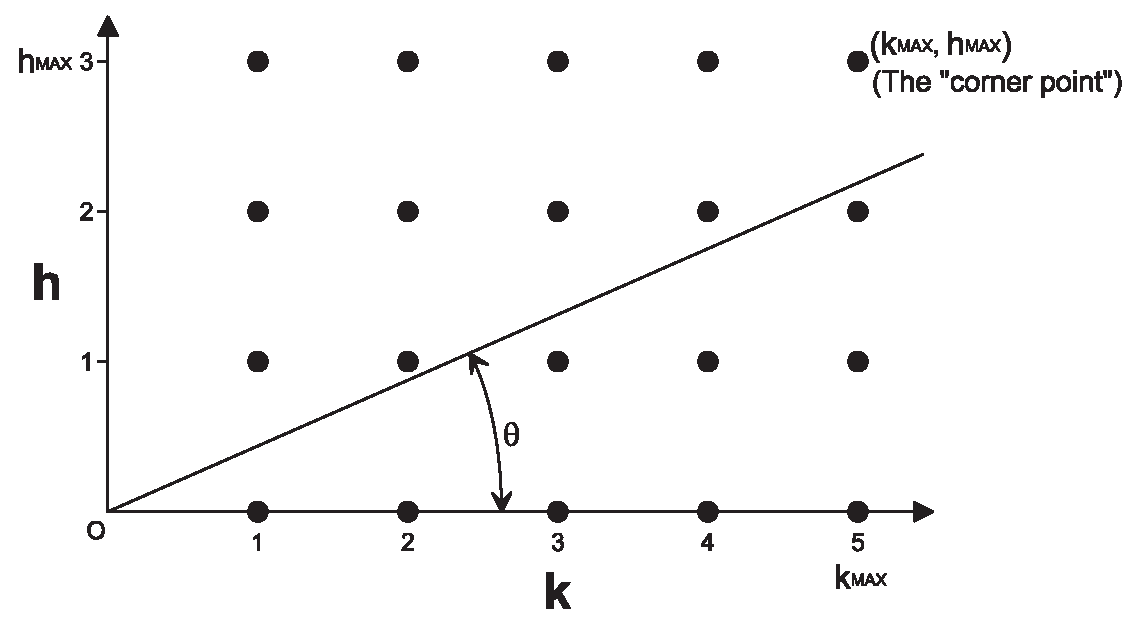
\includegraphics[width=4.6in]{c_fry0/farey01a.eps}
\caption{Graphical Interpretation Of Rational Numbers 
         $h/k$ That Can Be Formed With $h \leq h_{MAX}=3$, $k \leq k_{MAX}=5$}
\label{fig:cfry0:ili0:00}
\end{figure}

From the graphical interpretation suggested by Fig. \ref{fig:cfry0:ili0:00},
the following properties are intuitively clear.

\begin{itemize}
   \item The angle of a ray drawn from the origin to the point
         $(k,h)$ corresponding to the rational number $h/k$ is
         $\theta = tan^{-1} \; h/k$.

   \item Any integer lattice point on a line from 
         the origin drawn at the angle $\theta$
         has the value $h/k = tan \; \theta$.  All points corresponding
         to rational numbers with the same value will be on such a line,
         and thus form an equivalence class.

   \item A rational number $h/k$ is irreducible iff its corresponding
         point $(k,h)$ is ``directly'' visible from the origin with
         no intervening points.

   \item The Farey series of order $N$, $F_N$, can be 
         formed graphically by starting with the
		 set of integer lattice points
		 $(k,h): \; h \in \vworkintsetnonneg \wedge 1 \leq k \leq N$, 
		 then sweeping
         a line extended from the origin, starting with 
         angle $\theta = 0$, through
         $0 \leq \theta < \pi{}/2$, and recording 
         in order each point directly visible from
         the origin.\footnote{Note that Fig. \ref{fig:cfry0:ili0:00},
         because it illustrates the case when $h$ is constrained
         as well, does not show integer lattice points for
         $h > h_{MAX}$.  In principle, if the integer lattice shown
         in Fig. \ref{fig:cfry0:ili0:00} were extended indefinitely
         ``upward'', every positive irreducible rational number with
         $k \leq k_{MAX} = 5$ could be found graphically.}
\end{itemize}

Fig. \ref{fig:cfry0:chk0:01} illustrates the graphical construction method
of $F_5$.  Note that only integer lattice points which are directly
visible from the origin (with no intervening points) are selected.
(Fig. \ref{fig:cfry0:chk0:01}, like Fig. \ref{fig:cfry0:ili0:00},
shows the case of constrained $h$---the integer lattice should be
continued ``upward'' to construct the Farey series.)

\begin{figure}
\centering
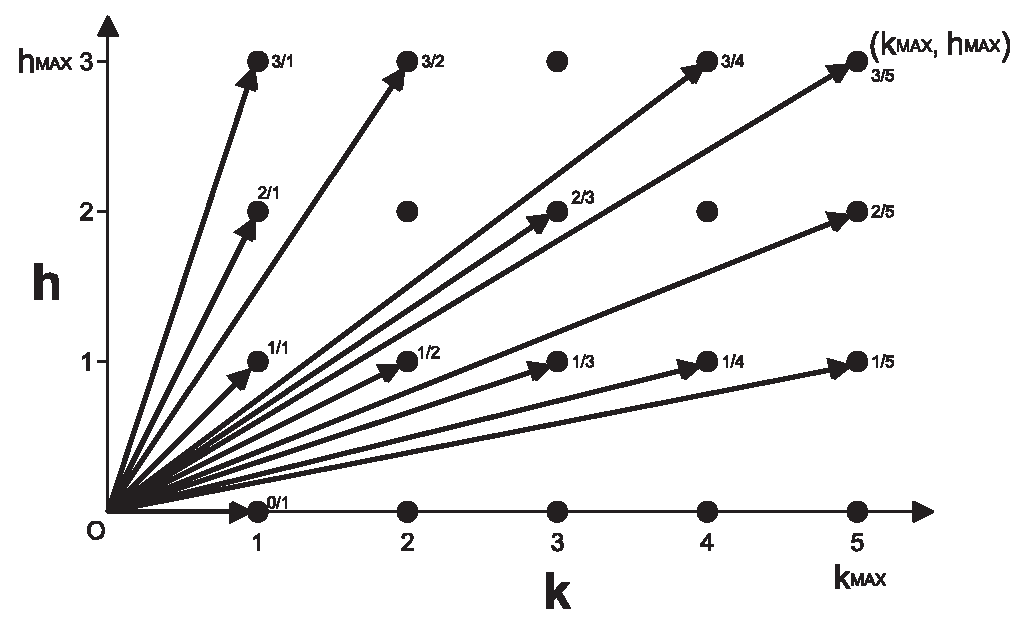
\includegraphics[width=4.6in]{c_fry0/farey01b.eps}
\caption{Graphical Interpretation Of Irreducible Rational Numbers 
         $h/k$ That Can Be Formed With $h \leq h_{MAX}=3$, $k \leq k_{MAX}=5$}
\label{fig:cfry0:chk0:01}
\end{figure}


%%%%%%%%%%%%%%%%%%%%%%%%%%%%%%%%%%%%%%%%%%%%%%%%%%%%%%%%%%%%%%%%%%%%%%%%%%%%%
%%%%%%%%%%%%%%%%%%%%%%%%%%%%%%%%%%%%%%%%%%%%%%%%%%%%%%%%%%%%%%%%%%%%%%%%%%%%%
%%%%%%%%%%%%%%%%%%%%%%%%%%%%%%%%%%%%%%%%%%%%%%%%%%%%%%%%%%%%%%%%%%%%%%%%%%%%%
\section[Generating $F_{k_{MAX}, \overline{h_{MAX}}}$ In A Rectangular Region]
        {Generating \mbox{\boldmath $F_{k_{MAX}, \overline{h_{MAX}}}$}
         Over A Rectangular Region Of The Integer Lattice}
%Section tag: CHK0
\label{cfry0:schk0}

\index{FKMAXHMAX@$F_{k_{MAX}, \overline{h_{MAX}}}$}
In practice, $F_N$ does not represent the set of
rational numbers that may be used for rational approximation in an
application; hence it isn't usually appropriate to choose a
rational number from $F_N$ strictly as
the theory of numbers defines it.  
An actual application is parameterized not just by
$k_{MAX}$ (the maximum denominator that may be chosen, which is considered
in the definition of the Farey series), 
but also by $h_{MAX}$ (the maximum numerator
that may be chosen).  Typically, $h_{MAX}$ exists as a constraint
because a machine multiplication instruction is limited in the size of the
operands it can accomodate; and $k_{MAX}$ exists as a constraint because
a machine division instruction is limited in the size of the divisor
it can accomodate.

In practice, the rational numbers that may be used for rational
approximation represent a rectangular region of the integer
lattice---all $(k,h):$ $h \leq h_{MAX} \wedge k \leq k_{MAX}$ 
(Figs. \ref{fig:cfry0:ili0:00}, \ref{fig:cfry0:chk0:01}).

Fig. \ref{fig:cfry0:ili0:00} supplies a graphical
interpretation of all rational numbers
that can be formed with constraints $h \leq h_{MAX} = 3$ 
and $k \leq k_{MAX} = 5$.  Each point of the integer lattice
shown in the figure is a rational number, not necessarily 
irreducible.  Because under this graphical interpretation
a rational number is irreducible iff it can be reached
by a ray from the origin with no intervening rational numbers,
it is clear that the complete ordered set of irreducible
rational numbers that can be formed under the
constraints $h \leq h_{MAX}$ and $k \leq k_{MAX}$
can be obtained graphically by sweeping a ray from
the origin through the angles $0 \leq \theta < \pi/2$,
recording each point directly visible from the origin.
This graphical construction process is illustrated
in Fig. \ref{fig:cfry0:chk0:01}.

From the graphical construction process shown in 
Fig. \ref{fig:cfry0:chk0:01}, it can be seen that the 
set of irreducible rational numbers that can be formed
subject to the constraints 
$h \leq h_{MAX} \wedge k \leq k_{MAX}$ is:

\begin{equation}
\left\{ { \frac{0}{1}, \frac{1}{5}, \frac{1}{4},
          \frac{1}{3}, \frac{2}{5}, \frac{1}{2},
          \frac{3}{5},
          \frac{2}{3}, \frac{3}{4}, \frac{1}{1},
          \frac{3}{2}, \frac{2}{1}, \frac{3}{1} } \right\} .
\end{equation}

We denote the ordered set of irreducible rational 
numbers that can be formed subject to the
constraints $h \leq h_{MAX} \wedge k \leq k_{MAX}$ as
$F_{k_{MAX}, \overline{h_{MAX}}}$.\footnote{Notationally,
in general,
we use an overbar on the order of a Farey series to
denote that the terms are inverted and reversed in order.
For example, $F_3 = \{ 0/1, 1/3, 1/2, \ldots \}$, but
$F_{\overline{3}}  = \{ \ldots , 2/1, 3/1 \}$.  Notation
such as $F_{A, \overline{B}}$ is an extension of that convention.}

There are three important questions to be asked about
the series $F_{k_{MAX}, \overline{h_{MAX}}}$:

\begin{itemize}
\item What are the smallest and largest rational numbers in
      $F_{k_{MAX}, \overline{h_{MAX}}}$?
      (This question is easy:  the smallest two rational numbers
	  in $F_{k_{MAX}, \overline{h_{MAX}}}$ are $0/1$
	  and $1/k_{MAX}$, and the largest rational number
	  is $h_{MAX}/1$.)

\item How do we construct $F_{k_{MAX}, \overline{h_{MAX}}}$?

\item If we desire to approximate a real number 
      $r_I$, $r_{IMIN} \leq r_I \leq r_{IMAX}$,
      using a rational number selected from 
	  $F_{k_{MAX}, \overline{h_{MAX}}}$, how large might
      the error $| h/k - r_I |$ be?
\end{itemize}


\subsection[Construction Of $F_{k_{MAX},\overline{h_{MAX}}}$]
           {Construction Of \mbox{\boldmath $F_{k_{MAX},\overline{h_{MAX}}}$}}

\index{FKMAXHMAX@$F_{k_{MAX}, \overline{h_{MAX}}}$!construction of}
To construct $F_{k_{MAX}, \overline{h_{MAX}}}$, for 
$0 \leq \theta \leq \tan^{-1} (h_{MAX}/k_{MAX})$---the 
region of the series where $k_{MAX}$ is the dominant constraint,
i.e. below the ``corner point'' in Figs. \ref{fig:cfry0:ili0:00}
and \ref{fig:cfry0:chk0:01}---note
that these terms are simply 
$F_{k_{MAX}}$ up to $h_{MAX}/k_{MAX}$ or its reduced 
equivalent.\footnote{If this is not intuitively clear,
note in Figs. \ref{fig:cfry0:ili0:00} and \ref{fig:cfry0:chk0:01}
that all of the terms of $F_{k_{MAX}}$---that is, all rational
numbers, both reducible and irreducible, with $k \leq k_{MAX}$---are 
available for selection
until the ``corner point'' is reached.}
To construct $F_{k_{MAX}, \overline{h_{MAX}}}$ for
$\tan^{-1} (h_{MAX}/k_{MAX}) < \theta < \pi/2$---the 
region of the series where $h_{MAX}$ is the dominant constraint,
i.e. above the ``corner point'' in Figs. \ref{fig:cfry0:ili0:00}
and \ref{fig:cfry0:chk0:01}---note that by a graphical argument
of symmetry, these terms are the reciprocals of ascending terms of $F_{h_{MAX}}$.
For example, in Fig. \ref{fig:cfry0:chk0:01}, if the $h$- and $k$-
axes are transposed, it is easy to see that $3/1$ in the original integer lattice
would correspond to $1/3$ in the transposed integer lattice.  This argument of
symmetry immediately suggests a procedure for constructing 
$F_{k_{MAX},\overline{h_{MAX}}}$.

\begin{itemize}
\item Construct $F_{k_{MAX}}$ from $0/1$ up through $h_{MAX}/k_{MAX}$ or its
      reduced equivalent.
\item Construct $F_{h_{MAX}}$ from $1/h_{MAX}$ up to $k_{MAX}/h_{MAX}$ or
      its reduced equivalent; then reverse the order of the 
	  terms and take the reciprocal of
      each term.
\item Concatenate the results from the two steps above.
\end{itemize}

\begin{vworkexamplestatement}
\label{ex:cfry0:schk:00}
Construct $F_{5,\overline{3}}$, the set of 
all irreducible rational numbers $h/k$
that can be formed with $h \leq h_{MAX}=3$ and 
$k \leq k_{MAX}=5$.\footnote{Note that $F_{5,\overline{3}}$
is the series depicted in Fig. \ref{fig:cfry0:chk0:01}, and
this example can be verified against the figure.}
\end{vworkexamplestatement}
\begin{vworkexampleparsection}{Solution}
(Using the method of construction presented above.)
First, $F_5$ up through $h_{MAX}/k_{MAX} = 3/5$ or its reduced
equivalent should be constructed.  This series is

\begin{equation}
\label{eq:cfry0:schk:ex00:eq00}
F_5 = 
\left\{ { \frac{0}{1}, \frac{1}{5}, \frac{1}{4},
          \frac{1}{3}, \frac{2}{5}, \frac{1}{2},
          \frac{3}{5}, \ldots{} } \right\} .
\end{equation}

Second, $F_3$ is constructed from $1/3$ up to $k_{MAX}/h_{MAX} = 5/3$ or
its reduced equivalent (not including the
final term, $5/3$).  This series is

\begin{equation}
\label{eq:cfry0:schk:ex00:eq01}
F_3 = 
\left\{ { \ldots , \frac{1}{3}, \frac{1}{2}, \frac{2}{3},
          \frac{1}{1}, \frac{4}{3}, \frac{3}{2}, \ldots{} } \right\} .
\end{equation}

Third, the terms of $F_3$ are reversed in order, and the reciprocal of each term is
calculated, yielding

\begin{equation}
\label{eq:cfry0:schk:ex00:eq02}
F_{\overline{3}} = 
\left\{ { \ldots{}, \frac{2}{3}, \frac{3}{4}, \frac{1}{1},
          \frac{3}{2}, \frac{2}{1}, \frac{3}{1}  } \right\} .
\end{equation}

Finally, concatenating (\ref{eq:cfry0:schk:ex00:eq00})
and
(\ref{eq:cfry0:schk:ex00:eq02}) yields $F_{5,\overline{3}}$, below.

\begin{equation}
\label{eq:cfry0:schk:ex00:eq03}
F_{5,\overline{3}} =
\left\{ { \frac{0}{1}, \frac{1}{5}, \frac{1}{4},
          \frac{1}{3}, \frac{2}{5}, \frac{1}{2},
          \frac{3}{5},
          \frac{2}{3}, \frac{3}{4}, \frac{1}{1},
          \frac{3}{2}, \frac{2}{1}, \frac{3}{1} } \right\}
\end{equation}

\end{vworkexampleparsection}
\vworkexamplefooter{}

It is clear that Thm. \ref{thm:cfry0:sgfs0:01}
and (\ref{eq:cfry0:sgfs0:thm:01:eq01}) through
(\ref{eq:cfry0:sgfs0:thm:01:eq04}) can be used to construct
$F_{k_{MAX}, \overline{h_{MAX}}}$.  However, such algorithms
are not discussed because---even with refinements---they
can be no better than $O(N)$ and are not
fruitful to develop.  Instead, an $O(log N)$
algorithm is presented in 
\ccfrzeroxrefcomma{}\ccfrzeromcclass{} \ref{ccfr0}, 
\emph{\ccfrzeroshorttitle{}}.


%%%%%%%%%%%%%%%%%%%%%%%%%%%%%%%%%%%%%%%%%%%%%%%%%%%%%%%%%%%%%%%%%%%%%%%%%%%%%
%%%%%%%%%%%%%%%%%%%%%%%%%%%%%%%%%%%%%%%%%%%%%%%%%%%%%%%%%%%%%%%%%%%%%%%%%%%%%
%%%%%%%%%%%%%%%%%%%%%%%%%%%%%%%%%%%%%%%%%%%%%%%%%%%%%%%%%%%%%%%%%%%%%%%%%%%%%
\subsection[Distance Between Terms Of $F_{h_{MAX},k_{MAX}}$]
           {Distance Between Terms Of \mbox{\boldmath $F_{h_{MAX},k_{MAX}}$}}

\index{FKMAXHMAX@$F_{k_{MAX}, \overline{h_{MAX}}}$!distance between terms}
\index{Farey series!distance between terms}
The maximum \emph{distance} between terms of $F_{h_{MAX},k_{MAX}}$ also establishes
what we call the maximum \emph{placement error}, $|r_A - r_I|$, in choosing
$r_A = h/k$.  Specifically, the maximum distance is twice the maximum placement
error.  Clearly, with a maximum distance specified, choosing $r_I = (x+y)/2$ for
two successive terms $x$ and $y$ separated by the maximum distance is 
the most antagonistic
choice of $r_I$ possible.
We use the two notions (maximum distance and maximum placement error)
interchangeably and don't bother to convert between them, as they are
the same notion and differ only by a factor of two.

It is clear from the earlier discussion of the Farey series that the maximum
distance between terms in $F_{k_{MAX}}$ is $1/k_{MAX}$, and that this maximum
distance occurs only adjacent to an integer.  It is also clear from the
discussion of $F_{\overline{h_{MAX}}}$ that the maximum distance between terms
is 1.

Thus, when we use $F_{k_{MAX}, \overline{h_{MAX}}}$ to approximate real numbers,
in general the worst-case distance between terms is 1.

In practical applications when rational approximation is used,
the approximation tends to be used over a restricted interval
$[l \gg  0, r \ll h_{MAX}]$ rather than over the full range of the rational numbers that
can be formed, $[0, h_{MAX}]$.  This section develops novel upper bounds on
the distance between terms of $F_{k_{MAX}, \overline{h_{MAX}}}$ in an interval
$[l,r]$.  For simplicity, assume $l,r \in F_{k_{MAX}, \overline{h_{MAX}}}$.

Three distinct cases are developed (Figure \ref{fig:cfry0:schk0:threecases}).
The upper bound developed from Case III is always larger than the upper
bound developed from Case II, which is always larger than the upper bound developed
from Case I; so if only the absolute maximum error over
the interval $[l,r]$ is of interest, only the
highest-numbered case which applies needs to be evaluated.  However, some
applications may have different error requirements in different regions
of the interval $[l,r]$, and for these applications it may be beneficial
to analyze more than one case.

\begin{figure}
\centering
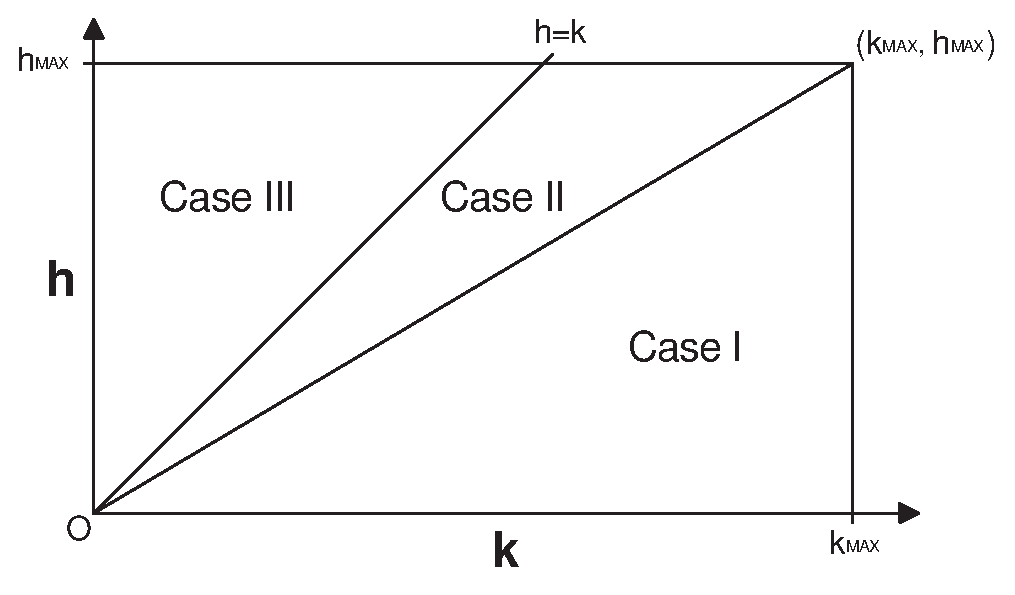
\includegraphics[width=4.6in]{c_fry0/errreg01.eps}
\caption{Three Cases For Bounding Distance Between Terms In 
         $F_{k_{MAX}, \overline{h_{MAX}}}$}
\label{fig:cfry0:schk0:threecases}
\end{figure}


\subsubsection[Case I:  $r_I < h_{MAX}/k_{MAX}$]
              {Case I:  \mbox{\boldmath $r_I < h_{MAX}/k_{MAX}$}}

With $r_I < h_{MAX}/k_{MAX}$, $k \leq k_{MAX}$ is the dominant
constraint, and the neighbors available to $r_I$ are simply the
terms of $F_{k_{MAX}}$.  If $[l, r] \cap  [0, h_{MAX}/k_{MAX}]$
includes an integer, clearly the maximum distance from $r_I$ to the
nearest available term of $F_{k_{MAX}, \overline{h_{MAX}}}$ is given
by

\begin{equation}
\left|
\frac{h}{k} - r_I
\right|
\leq
\frac{1}{2 k_{MAX}} ,
\end{equation}

which is the same result for the Farey series in general.

If $[l, r] \cap  [0, h_{MAX}/k_{MAX}]$ does
not include an integer, it can be shown that the
maximum distance between Farey terms is driven by the
rational number with the smallest denominator in the
interval $[l, r]$.

For two consecutive terms $p/q$ and $p'/q'$ in $F_{k_{MAX}}$,
$p'q - pq' = 1$ (Thm. \ref{thm:cfry0:spfs:02}), so that

\begin{equation}
\frac{p'}{q'} - \frac{p}{q} =
\frac{p'q - pq'}{q q'} = \frac{1}{qq'} .
\end{equation}

By Thm. \ref{thm:cfry0:spfs:02ba}, $q+q' > k_{MAX}$, therefore

\begin{equation}
\label{eq:cfry0:schk0:minqplacementupperbound}
\frac{1}{q k_{MAX}} \leq
\frac{1}{q q'} <
\frac{1}{q (k_{MAX}-q)}.
\end{equation}

Let $q_{MIN}$ be the smallest denominator of any rational number
$\in F_{k_{MAX}}$ in the interval $[l,r]$.  It is then easy to show
that for any consecutive denominators $q, q'$ which occur in
$F_{k_{MAX}}$ in the interval $[l,r]$,

\begin{equation}
\frac{1}{q q'} < \frac{1}{q_{MIN} \; max (q_{MIN}, k_{MAX} - q_{MIN})} .
\end{equation}

Thus, the upper bound on the distance between consecutive terms of $F_{k_{MAX}}$
in an interval $[l,r]$ is tied to the minimum denominator of any
rational number $\in F_{k_{MAX}}$ in $[l,r]$.

Note that clearly
$q_{MIN} \leq 1/(r-l)$, so for most practical intervals $[l,r]$,
the search for $q_{MIN}$ would not be computationally expensive.
However, applications could arise where an approximation is used
in an \emph{extremely} narrow interval, and having an algorithm available that
is computationally viable for such cases is advantageous.  For example,
locating the rational number $\in F_{2^{20,000}}$ with the smallest denominator
in an interval of width $2^{-10,000}$ could be a serious computational
problem.

To locate $q_{MIN}$ in $[l,r]$, note that at least one rational number
with $q_{MIN}$ as a denominator in $[l,r]$ is the best approximation
of order $q_{MIN}$ to the midpoint of the interval,
$(l+r)/2$.\footnote{Thanks to David M. Einstein \cite{bibref:i:davidmeinstein} 
and David Eppstein \cite{bibref:i:davideppstein}
for this observation, contributed via the \texttt{sci.math} newsgroup
\cite{bibref:n:scimathnewsgroup},
which is the linchpin of Algorithm \ref{alg:cfmindenominator}.}
By theorem (\cite{bibref:b:KhinchinClassic}, Theorem 15), every best approximation
of a number is a convergent or intermediate fraction of the
continued fraction representation of the number.  We seek the
convergent or intermediate fraction of $(l+r)/2$ with the smallest
denominator that is in the interval $[l,r]$.\footnote{Regrettably,
at this point the cart comes before the horse---the insight and
algorithms which follow are based on continued fractions, which
are not covered until \ccfrzeroxrefcomma{}\ccfrzeromcclass{} \ref{ccfr0}, 
\emph{\ccfrzeroshorttitle{}}.  We apologize for the potential necessity
of reading this work out of order.}

The convergents and intermediate fractions of $(l+r)/2$ are naturally
arranged in order of increasing denominator.  However, it would be
inefficient to test \emph{every} intermediate fraction
for membership in $[l,r]$, as partial quotients $a_k$ are unlimited in
size and such an algorithm may not be $O(log \; k_{MAX})$.  Instead,
since intermediate fractions are formed using the parameterized
expression $(i p_k + p_{k-1})/(i q_k + q_{k-1})$,
and since intermediate fractions are ever-increasing
or ever-decreasing with respect to the parameter $i$, the
smallest value of $i$ which will create an intermediate
fraction potentially within $[l,r]$ can be directly
calculated.  Only the intermediate fraction formed with
this calculated value of $i$ needs to be tested for membership in
$[l,r]$.

Let $l_N$ and $l_D$ be the numerator and denominator of $l$, and
let $r_N$ and $r_D$ be the numerator and denominator of $r$.
In the case of $k$ even; $s_k < l < (l+r)/2$ (otherwise $s_k$
would have been identified as $\in [l,r]$, see Algorithm
\ref{alg:cfmindenominator}); $s_{k+1} \geq (l+r)/2$;
with increasing $i$, $(i p_k + p_{k-1})/(i q_k + q_{k-1})$
forms a decreasing sequence; and the inequality we seek to solve is

\begin{equation}
\label{eq:cfry0:schk0:ifselection01}
\frac{i p_k + p_{k-1}}{i q_k + q_{k-1}} \leq \frac{r_N}{r_D}.
\end{equation}

Solving (\ref{eq:cfry0:schk0:ifselection01}), the smallest integral 
value of $i$ that will suffice is

\begin{equation}
\label{eq:cfry0:schk0:ifselection02}
i = \left\lceil {
\frac{r_N q_{k-1} - r_D p_{k-1}}{r_D p_k - r_N q_k}
} \right\rceil .
\end{equation}

Similarly, for $k$ odd, the sequence is increasing,
and the inequality and solution are

\begin{equation}
\label{eq:cfry0:schk0:ifselection03}
\frac{i p_k + p_{k-1}}{i q_k + q_{k-1}} \geq \frac{l_N}{l_D}
\to
i = \left\lceil {
\frac{l_N q_{k-1} - l_D p_{k-1}}{l_D p_k - l_N q_k}
} \right\rceil .
\end{equation}

(\ref{eq:cfry0:schk0:ifselection01}),
(\ref{eq:cfry0:schk0:ifselection02}),
and (\ref{eq:cfry0:schk0:ifselection03}) suggest the following continued fraction
algorithm for finding
a rational number with the smallest denominator in an
interval $[l,r]$.

\begin{vworkalgorithmstatement}\label{alg:cfmindenominator}\end{vworkalgorithmstatement}
\begin{alglvl0}
\item Calculate all partial quotients $a_k$ and all convergents
      $s_k = p_k/q_k$ of the midpoint of the interval,
      $(l+r)/2$.

\item  For each convergent $s_k=p_k/q_k$, in order of increasing $k$:

   \begin{alglvl1}

   \item If $s_k = p_k/q_k \in [l,r]$, $s_k$ is a rational number with
         the lowest denominator, STOP.

   \item If $k$ is even,

      \begin{alglvl2}

      \item Calculate $i$ according to (\ref{eq:cfry0:schk0:ifselection02}).
            If $i < a_{k+1}$ and the intermediate fraction
            $(i p_k + p_{k-1})$ $/$ $(i q_k + q_{k-1})$ $\geq$ $l$, this intermediate
            fraction is
            a rational number with the lowest denominator, STOP.

      \end{alglvl2}

   \item Else if $k$ is odd,

      \begin{alglvl2}

      \item Calculate $i$ according to (\ref{eq:cfry0:schk0:ifselection03}).
            If $i < a_{k+1}$ and the intermediate fraction
            $(i p_k + p_{k-1})$ $/$ $(i q_k + q_{k-1})$ $\leq$ $r$, this intermediate
            fraction is
            a rational number with the lowest denominator, STOP.

      \end{alglvl2}

   \end{alglvl1}

\end{alglvl0}

Algorithm \ref{alg:cfmindenominator} is approximately $O(log \; k_{MAX})$,
since there are a fixed number of steps per convergent, and the maximum number
of convergents is $O(log \; k_{MAX})$.  Once a rational number with the smallest
denominator $q_{MIN}$ is located, (\ref{eq:cfry0:schk0:minqplacementupperbound})
can be applied to bound $|r_A - r_I|$; namely,

\begin{equation}
\label{eq:qminmaxplacementerror}
\left| {\frac{h}{k} - r_I}  \right|
<
\frac{1}{2q_{MIN} \; max(q_{MIN}, k_{MAX} - q_{MIN})} .
\end{equation}


%%%%%%%%%%%%%%%%%%%%%%%%%%%%%%%%%%%%%%%%%%%%%%%%%%%%%%%%%%%%%%%%%%%%%%%%%%%%%
%%%%%%%%%%%%%%%%%%%%%%%%%%%%%%%%%%%%%%%%%%%%%%%%%%%%%%%%%%%%%%%%%%%%%%%%%%%%%
%%%%%%%%%%%%%%%%%%%%%%%%%%%%%%%%%%%%%%%%%%%%%%%%%%%%%%%%%%%%%%%%%%%%%%%%%%%%%
\subsubsection[Case II:  $h_{MAX}/k_{MAX} < r_I < 1$]
              {Case II:  \mbox{\boldmath $h_{MAX}/k_{MAX} < r_I < 1$}}

If $h_{MAX}/k_{MAX} < r_I < 1$, a graphical argument
(Figure \ref{fig:cfry0:schk0:caseii}) can be used
to more tightly bound the maximum distance between terms of
$F_{k_{MAX}, \overline{h_{MAX}}}$.

\begin{figure}
\centering
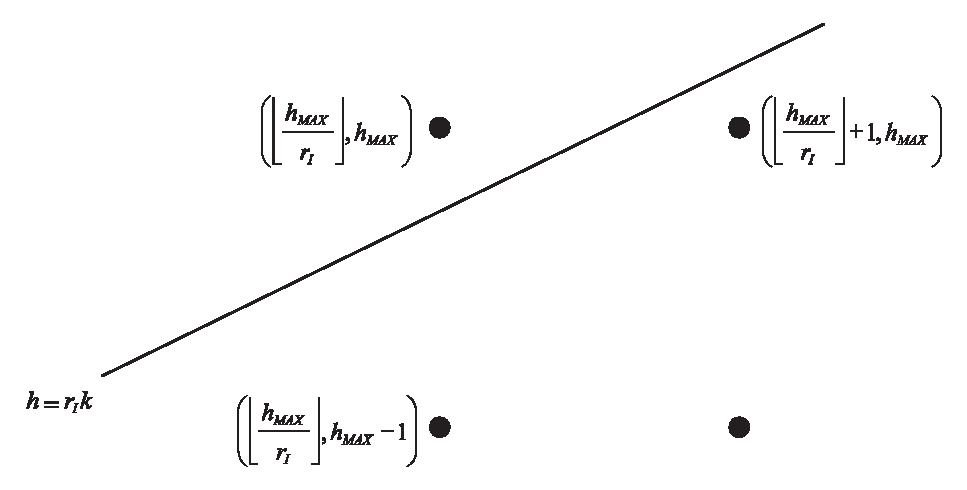
\includegraphics[height=2.0in]{c_fry0/errcase2.eps}
\caption{Graphical Interpretation Of Case II:  $h_{MAX}/k_{MAX} < r_I < 1$}
\label{fig:cfry0:schk0:caseii}
\end{figure}

In this case,  a formable term at or to the left\footnote{To the left on the
number line, but to the right in Figure \ref{fig:cfry0:schk0:caseii}.}
of $r_I$ is represented by the point $(\lfloor h_{MAX}/r_I \rfloor + 1, h_{MAX} )$
in the integer lattice,
and a formable term at or to the right of $r_I$ is
represented by the point $(\lfloor h_{MAX}/r_I \rfloor, h_{MAX} )$
in the integer lattice.  Thus, the maximum distance between
neighboring terms in $F_{k_{MAX}, \overline{h_{MAX}}}$
is given by the difference of these two terms,

\begin{equation}
\frac{h_{MAX}}{\left\lfloor {\frac{h_{MAX}}{r_I}} \right\rfloor}
-
\frac{h_{MAX}}{\left\lfloor {\frac{h_{MAX}}{r_I}} \right\rfloor + 1}
=
\frac{h_{MAX}}{{\left\lfloor {\frac{h_{MAX}}{r_I}} \right\rfloor}^2
+ \left\lfloor {\frac{h_{MAX}}{r_I}} \right\rfloor},
\end{equation}

and the maximum distance from $r_I$ to a neighboring term is
given by

\begin{equation}
\label{eq:cfry0:schk0:caseiimaxplacementerror}
\left|
\frac{h}{k} - r_I
\right|
\leq
\frac{h_{MAX}}{2 \left( { {\left\lfloor {\frac{h_{MAX}}{r_I}} \right\rfloor}^2
+ \left\lfloor {\frac{h_{MAX}}{r_I}} \right\rfloor } \right) }.
\end{equation}

Note that Case II will exist only if $h_{MAX}/k_{MAX} < 1$.


\subsubsection[Case III:  $1 < h_{MAX}/k_{MAX} < r_I$]
              {Case III:  \mbox{\boldmath $1 < h_{MAX}/k_{MAX} < r_I$}}

It can be established graphically, using the coordinate system of
Figure \ref{fig:cfry0:ili0:00}, Figure \ref{fig:cfry0:chk0:01},
or Figure \ref{fig:cfry0:schk0:threecases}, 
that the line $h=r_I k$ intercepts the
line $h=h_{MAX}$ at the point $(h_{MAX}/r_I, h_{MAX})$.  It is clear
from a graphical argument that all of the terms of the Farey series
of order $\lfloor h_{MAX}/r_I \rfloor$ are available as neighbors
of $r_I$.  Therefore,

\begin{equation}
\label{eq:cfry0:schk0:caseiiiplacementerror}
\left|
\frac{h}{k} - r_I
\right|
\leq
\frac{1}{2 \left\lfloor \frac{h_{MAX}}{r_I} \right\rfloor}.
\end{equation}


%%%%%%%%%%%%%%%%%%%%%%%%%%%%%%%%%%%%%%%%%%%%%%%%%%%%%%%%%%%%%%%%%%%%%%%%%%%%%
%%%%%%%%%%%%%%%%%%%%%%%%%%%%%%%%%%%%%%%%%%%%%%%%%%%%%%%%%%%%%%%%%%%%%%%%%%%%%
%%%%%%%%%%%%%%%%%%%%%%%%%%%%%%%%%%%%%%%%%%%%%%%%%%%%%%%%%%%%%%%%%%%%%%%%%%%%%
\section{Acknowledgements}
%Section tag: ACK0

This chapter is the result of work on inexpensive microcontroller 
arithmetic (and a paper) undertaken in 2000.
We would like to gratefully acknowledge the assistance
of 
\index{Bachelis, Greg}      Greg Bachelis     \cite{bibref:i:gregbachelis}, 
\index{Berman, Robert}      Robert Berman     \cite{bibref:i:robertberman}, 
\index{Lin, Feng}           Feng Lin          \cite{bibref:i:fenglin}, 
\index{Sahinidis, Nick}     Nick Sahinidis    \cite{bibref:i:nicksahinidis}, 
\index{Van Tuyl, Adam}      Adam Van Tuyl     \cite{bibref:i:adamvantuyl},
\index{Schweiger, Carl}     Carl Schweiger    \cite{bibref:i:carlschweiger}, 
\index{Tindell, Ken}        Ken Tindell       \cite{bibref:i:kentindell},
\index{Vestal, Steve}       Steve Vestal      \cite{bibref:i:stevevestal},
\index{Whitinger, Bob}      Bob Whitinger     \cite{bibref:i:bobwhitinger},
and 
\index{Stewart, David B.}   David B. Stewart   \cite{bibref:i:davidbstewart}
in finding the areas of
mathematics relevant to the rational number selection
problem.  We would also like to
thank 
\index{Bengtsson, Johan}    Johan Bengtsson    \cite{bibref:i:johanbengtsson},
\index{Burke, Michael J.}   Michael J. Burke   \cite{bibref:i:michaeljburke},  
\index{Endicott, Mark}      Mark Endicott      \cite{bibref:i:markendicott}, 
\index{Eppstein, David}     David Eppstein     \cite{bibref:i:davideppstein}, 
\index{Munteanu, Mircea}    Mircea Munteanu    \cite{bibref:i:mirceamunteanu},
\index{Gibson, Adam}        Adam Gibson        \cite{bibref:i:adamgibson}, 
and \index{Virgil}          Virgil             \cite{bibref:i:virgil}
(of the \index{sci.math.num-analysis@\texttt{sci.math.num-analysis} newsgroup}%
\texttt{sci.math.num-analysis} newsgroup 
\cite{bibref:n:scimathnumanalysis})
for insight into this problem; 
\index{Stallings, Cliff}    Cliff Stallings    \cite{bibref:i:cliffstallings}
and
\index{Kakos, Robert}       Robert Kakos       \cite{bibref:i:robertkakos}
for support from Wayne State
University's College Of Engineering; 
\index{Groen, Paulette}     Paulette Groen     \cite{bibref:i:paulettegroen}
and
\index{Smith, Paula}        Paula Smith        \cite{bibref:i:paulasmith}
for support from \index{Visteon}Visteon;
\index{Crosby, Bob}         Bob Crosby         \cite{bibref:i:bobcrosby}
for support
from \index{Texas Instruments}Texas Instruments; 
\index{Zauner, Klaus-Peter} Klaus-Peter Zauner  \cite{bibref:i:klauspeterzauner},
\index{Blome, Andrea}       Andrea Blome        \cite{bibref:i:andreablome},
\index{Smith, Una}          Una Smith           \cite{bibref:i:unasmith},
\index{Tinnefeld, Karsten}  Karsten Tinnefeld   \cite{bibref:i:karstentinnefeld},
and
\index{Franke, Axel}        Axel Franke         \cite{bibref:i:axelfranke}
for other tool
and logistical support; and the management
team at Visteon for allowing us to pursue this
effort in the workplace.


%%%%%%%%%%%%%%%%%%%%%%%%%%%%%%%%%%%%%%%%%%%%%%%%%%%%%%%%%%%%%%%%%%%%%%%%%%%%%
%%%%%%%%%%%%%%%%%%%%%%%%%%%%%%%%%%%%%%%%%%%%%%%%%%%%%%%%%%%%%%%%%%%%%%%%%%%%%
%%%%%%%%%%%%%%%%%%%%%%%%%%%%%%%%%%%%%%%%%%%%%%%%%%%%%%%%%%%%%%%%%%%%%%%%%%%%%
\section{Exercises}
%Section tag: EXE0

\begin{vworkexercisestatement}
\label{exe:cfry0:sexe0:01}
Prove that Theorem \ref{thm:cfry0:spfs:01}
holds in the degenerate cases where $h=1$ and where $k=1$.
\end{vworkexercisestatement}
\vworkexercisefooter{}

\begin{vworkexercisestatement}
\label{exe:cfry0:sexe0:02}
Prove that Theorem \ref{thm:cfry0:spfs:01} holds $\forall i \in \vworkintset$
(rather than $\forall i \in \vworkintsetnonneg$) using
the slightly amended notion of reducibility that $h/k$ is irreducible iff
$\lfloor h \rfloor / k$ is irreducible.
\end{vworkexercisestatement}
\vworkexercisefooter{}

\begin{vworkexercisestatement}
In Section \ref{cfry0:sgfs0} and Algorithm \ref{alg:cfry0:sgfs0:02}
it is stated that for $i \in \vworkintsetnonneg$, 
$(iN-1)/N$, $i/1$, and $(iN+1)/N$ are consecutive terms in the Farey series
or order $N$, $F_N$.  Prove that $(iN-1)/N$ and $(iN+1)/N$ are irreducible,
and the left and right Farey neighbors to $i/1$.
\end{vworkexercisestatement}
\vworkexercisefooter{}

\begin{vworkexercisestatement}
Prove that in $F_N$ the maximum distance between terms $1/N$ can occur
only adjacent to an integer.
\end{vworkexercisestatement}
\vworkexercisefooter{}


%%%%%%%%%%%%%%%%%%%%%%%%%%%%%%%%%%%%%%%%%%%%%%%%%%%%%%%%%%%%%%%%%%%%%%%%%%

\noindent\begin{figure}[!b]
\noindent\rule[-0.25in]{\textwidth}{1pt}
\begin{tiny}
\begin{verbatim}
$HeadURL: svn://localhost/dtapublic/pubs/books/ucbka/trunk/c_fry0/c_fry0.tex $
$Revision: 277 $
$Date: 2019-08-12 22:35:39 -0400 (Mon, 12 Aug 2019) $
$Author: dashley $
\end{verbatim}
\end{tiny}
\noindent\rule[0.25in]{\textwidth}{1pt}
\end{figure}

%%%%%%%%%%%%%%%%%%%%%%%%%%%%%%%%%%%%%%%%%%%%%%%%%%%%%%%%%%%%%%%%%%%%%%%%%%
%
%End of file C_FRY0.TEX


%Chapter:  Continued Fractions And Related Topics
%$Header: svn://localhost/dtapublic/pubs/books/ucbka/trunk/c_cfr0/c_cfr0.tex 275 2019-08-12 00:47:10Z dashley $

\chapter{\ccfrzerolongtitle{}}

\label{ccfr0}

\beginchapterquote{``I began by saying that there is probably less difference
                     between the positions of a mathematician and a physicist
                     than is generally supposed, and that the most important
                     seems to me to be this, that the mathematician is in much
                     more direct contact with reality \ldots{} mathematical
                     objects are so much more what they seem.  A chair or a
                     star is not in the least what it seems to be; the more we think
                     of it, the fuzzier its outlines become in the haze of sensation
                     which surround it; but `2' or `317' has nothing to do with
                     sensation, and its properties stand out the more clearly the more
                     closely we scrutinize it.''}
                     {G. H. Hardy \cite{bibref:b:mathematiciansapology:1940}, pp. 128-130}
					 \index{Hardy, G. H.}

%%%%%%%%%%%%%%%%%%%%%%%%%%%%%%%%%%%%%%%%%%%%%%%%%%%%%%%%%%%%%%%%%%%%%%%%%%%%%
%%%%%%%%%%%%%%%%%%%%%%%%%%%%%%%%%%%%%%%%%%%%%%%%%%%%%%%%%%%%%%%%%%%%%%%%%%%%%
%%%%%%%%%%%%%%%%%%%%%%%%%%%%%%%%%%%%%%%%%%%%%%%%%%%%%%%%%%%%%%%%%%%%%%%%%%%%%
\section{Introduction}
%Section tag: INT0
\label{ccfr0:sint0}
\index{continued fraction}
\index{continued fraction!definition}

A \emph{finite simple continued fraction} is a fraction of the form

\begin{equation}
\label{eq:ccfr0:int0:00}
a_0 + \cfrac{1}{a_1 + \cfrac{1}{a_2
    + \cfrac{1}{\;\;\;\;\;\;\;\;\;\;\;\;\;\;\ldots + \cfrac{1}{a_n}}}}
    =
    [a_0; a_1, a_2, \ldots , a_n] ,
\end{equation}

\noindent{}where $a_0 \in \vworkintsetnonneg$ and 
$a_i \in \vworkintsetpos$, $i > 0$.  Each integer
$a_i$ is called an \index{continued fraction!element}\emph{element} or
\index{continued fraction!partial quotient}\emph{partial quotient} 
of the continued fraction.
We require, except in the case of
the continued fraction representation of an integer,
that the final element $a_n$ not be equal
to 1.\footnote{\label{footnote:ccfr0:sint0:00}The reason for 
this restriction is discussed later.}

Continued fractions are quite unwieldly to write and typeset,
and so a continued fraction in the form of (\ref{eq:ccfr0:int0:00})
is written as $[a_0; a_1, a_2, \ldots , a_n]$.  Note that the
separator between $a_0$ and $a_1$ is a semicolon (`;'), and that all other
separators are commas (`,').  In some works, commas are used exclusively; and in
other works, the first element is $a_1$ rather than $a_0$.  Throughout this
work, the notational conventions illustrated in (\ref{eq:ccfr0:int0:00}) are
followed.

In this chapter, the framework of continued fractions is presented in the
context of finding rational numbers in $F_N$, the Farey series of order $N$,
enclosing an arbitrary $r_I \in \vworkrealsetnonneg$.  The continued fraction
algorithm presented (Algorithm \ref{alg:ccfr0:scba0:cfenclosingneighborsfn})
is $O(log N)$, and so is suitable for finding the best rational
approximations in $F_N$ even when $N$ is very large.  Because our emphasis 
is on practical applications rather than number theory, we don't include more
information than is necessary to understand the applications we have in 
mind.

The study of continued
fractions is a topic from number theory (a branch of mathematics).  It may be
counterintuitive to anyone but a number theorist that continued fractions
can be used to economically find best rational approximations, 
or that continued fractions are anything but
a parlor curiosity.  C.D. Olds (\cite{bibref:b:OldsClassic}, p. 3) comments:

\index{Olds, C. D.}

\begin{quote}
At first glance, nothing seems simpler or less significant than writing a number,
for example $\frac{9}{7}$, in the form

\begin{equation}
\frac{9}{7} = 1 + \frac{2}{7} = 1 + \frac{1}{\cfrac{7}{2}}
            = 1 + \cfrac{1}{3 + \cfrac{1}{2}}
            = 1 + \cfrac{1}{3 + \cfrac{1}{1 + \cfrac{1}{1}}}.
\end{equation}

It turns out, however, that fractions of this form, called ``continued
fractions'', provide much insight into mathematical problems, particularly into
the nature of numbers.

Continued fractions were studied by the great mathematicians of the seventeenth
and eighteenth centuries and are a subject of active investigation today.
\end{quote}


%%%%%%%%%%%%%%%%%%%%%%%%%%%%%%%%%%%%%%%%%%%%%%%%%%%%%%%%%%%%%%%%%%%%%%%%%%%%%
%%%%%%%%%%%%%%%%%%%%%%%%%%%%%%%%%%%%%%%%%%%%%%%%%%%%%%%%%%%%%%%%%%%%%%%%%%%%%
%%%%%%%%%%%%%%%%%%%%%%%%%%%%%%%%%%%%%%%%%%%%%%%%%%%%%%%%%%%%%%%%%%%%%%%%%%%%%
\section{History Of Continued Fractions}
%Section tag: HST0
\label{cfr0:hst0}
\index{continued fraction!history of}

The only work we are aware of that explicitly treats the history
of continued fractions is \cite{bibref:b:HistoryCfPadeApproxBrezinski}.
Although the history of continued fractions is complex,
two points are clear.  First, it is clear that Euclid's \index{Euclid}
GCD algorithm \index{Euclid!GCD algorithm}
(Algorithm \ref{alg:ccfr0:sega0:euclidsgcdalgorithm}),
which was known no later than around 300 B.C., 
represents the historical origin of the continued fraction.  Second,
it is clear that the utility of the apparatus of continued fractions
in finding best rational approximations---specifically the properties
of convergents---was understood by the 17th century. 

In this section, we present some excerpts from 
\cite{bibref:b:HistoryCfPadeApproxBrezinski}
which show the very early use of continued fractions to obtain best rational
approximations with a numerator and denominator less than certain
prescribed limits.
We simply demonstrate that the technique we present was known by
the 17th century (with the possible exception of the 
second component of Theorem \ref{thm:ccfr0:scba0:cfenclosingneighbors}),
and we don't attempt to describe the other uses
of continued fractions or the significance of continued fractions
in mathematics or number theory.

Although we present best rational
approximations in the context of being able to effectively use
processor integer multiplication and division instructions,
earlier historical work was aimed at either
providing rational approximations to irrational numbers ($\sqrt{2}$ or $\pi$,
for example), or at determining optimal numbers of gear teeth 
(in mechanical systems).  Naturally, the need for best rational approximations
in the context of computer arithmetic is a relatively recent
development.

In the introduction of \cite{bibref:b:HistoryCfPadeApproxBrezinski},
Brezinski \index{Brezenski, Claude} hints at the broad application and importance
of continued fractions:

\begin{quote}
The history of continued fractions is certainly one of the longest
among those of mathematical concepts, since it begins with
Euclid's algorithm \index{Euclid!GCD algorithm} for the greatest common divisor at least
three centuries B.C.  As it is often the case and like
Monsieur Jourdain in Moli\`ere's ``le bourgeois gentilhomme''
(who was speaking in prose though he did not know he was doing so), 
continued fractions were used for many centuries before their real
discovery.

The history of continued fractions and Pad\'e approximants is also
quite important, since they played a leading role in the development
of some branches of mathematics.  For example, they were the basis
for the proof of the transcendence of $\pi$ in 1882, an open
problem for more than two thousand years, and also for our modern
spectral theory of operators.  Actually they still are of great
interest in many fields of pure and applied mathematics and in
numerical analysis, where they provide computer approximations to
special functions and are connected to some convergence acceleration
methods.  Continued fractions are also used in number theory,
computer science, automata, electronics, etc. \ldots{}
\end{quote}

Notice that Theorem \ref{thm:ccfr0:scba0:cfenclosingneighbors} 
has two components.  First, it is shown that the highest-order
convergent with an acceptable denominator is closer to $a/b$ than
any Farey neighbor to this convergent (thus, this convergent must be
either a left or right  Farey neighbor of $a/b$).  Second, it is shown
what the other Farey neighbor must be.  It is historically clear
that the properties of convergents as best rational approximations were
understood by the 17th century (this is the \emph{first} part of
Theorem \ref{thm:ccfr0:scba0:cfenclosingneighbors}).  However, it
is not historically clear when the \emph{second} part of
Theorem \ref{thm:ccfr0:scba0:cfenclosingneighbors} was discovered.

Even in Khinchin's \index{Khinchin, A. Ya.} classic work, 
\cite{bibref:b:KhinchinClassic}, Theorem 15, p. 22, Khinchin stops
just short of the result presented as the second part of
Theorem \ref{thm:ccfr0:scba0:cfenclosingneighbors}.  Khinchin writes:

\begin{quote}
THEOREM 15.  \em Every best approximation of a number is a convergent
or an intermediate fraction of the continued fraction representing
that number.
\end{quote}

\noindent{}Theorem \ref{thm:ccfr0:scba0:cfenclosingneighbors} goes 
slightly farther than Khinchin's \emph{THEOREM 15}, above.  
Khinchin \index{Khinchin, A. Ya.} states
that a best approximation will be a convergent or an intermediate 
fraction---but Theorem \ref{thm:ccfr0:scba0:cfenclosingneighbors}
goes slightly farther to indicate \emph{exactly which} intermediate fraction
is potentially the best approximation.  Khinchin's \emph{THEOREM 15}
is correct, but could be strengthened.  Khinchin's work 
was first published in 1935.  This raises the [unlikely] possibility
that the second part of Theorem \ref{thm:ccfr0:scba0:cfenclosingneighbors}
had not been published even as recently as 1935, although
we (the authors) don't have the ability to confirm or
refute this.

In \cite{bibref:b:HistoryCfPadeApproxBrezinski}, p. 70, Brezinski
\index{Brezenski, Claude}
writes:

\begin{quote}
In the same period, algorithms equivalent to continued fractions were
still used to find approximate values for ratios and to simplify
fractions.  We have already mentioned Albert Girard.

Among the other authors who treated the subject, the most prominent
is Daniel SCHWENTER \index{Schwenter, Daniel}
(N\"urnberg, 31.1.1585 - Altdorf, 19.1.1636),
who wrote two books ``\emph{Geometriae practicae novae et auctae
tractatus}'' published in 1627 and ``\emph{Delicae
Physico-mathematicae}'' which appeared in 1636 followed by a
second edition in 1651.

In his first book, Schwenter found approximations of 177/233 by
finding their g.c.d. and gave the successive convergents
79/104, 19/25, 3/4, 1/1, and 0/1.  His calculations were arranged
in a table\footnote{The table is reproduced in 
\cite{bibref:b:HistoryCfPadeApproxBrezinski}, 
but is omitted here.} \ldots{} although he gave no explanation of the method.
\end{quote}

On p. 84, Brezenski \index{Brezenski, Claude} writes:

\begin{quote}
Wallis \index{Wallis, John} also made use of continued fractions in his book
``\emph{A treatise of algebra both historical and practical}''
(published in 1685), to approximate ratios with large
numerators and denominators:

\emph{``Before I leave the business of Decimal Parts, and the 
advantages which in practice may there cause; I have thought fit 
here to insert a Process Of Reducing Fractions or Proportions to
smaller termes, retaining as near as may be, the just value.}

\emph{It was occasion'd by a Problem sent me (as I remember) about the
Year 1663 or 1664, by Dr. Lamplugh the present Bishop of Exeter from
(his Wives Father) Dr. Davenant then one of the Prebends
Residentaries of the Church of Salisbury, a very worthy Person, of
great Learning and Modesty; as I mire inderstand from persons
well acquainted with him, and by divers Writings of his which I have seen,
though I never had the opportunity of being personally acquainted with him,
otherwise than by Letter.  And amongst
his other Learning, he was very well skilled the Mathematicks,
and a diligent Proficient therein.}

\emph{He sent me (as it abovesaid) a Fraction (which what it was I 
do not now particulary remember) who's Numerator and Denominator
were, each of them of about six or seven places; and Proposed to
find the nearest Fraction in value to it, whose Denominator should
not be greater than 999.''}

\begin{center}
\rule{3in}{0.3mm}  \\\
\end{center}

\begin{center}
\emph{The Problem} \\
\end{center}

\emph{A Fraction (or Proportion) being assigned, to sind one as near as 
may be equal to it, in Numbers non exceeding a Number given, and in
the smallest Terms.}

\emph{As (for instance), the Fraction $\frac{2684769}{8376571}$ (or the
Proportion of 2684769 to 8376571) being assigned, to sind one equal to it
(if it may be) or at least the next Greater, or the next Lesser,
which may be expressed in Numbers not greater than 999; that is, in numbers
not exceeding three places.}

\begin{center}
\rule{3in}{0.3mm}  \\
\end{center}

\emph{If the Fraction sought (whose terms are not to be greater than
a Number given) be the Next Greater than a Fraction Proposed; divide the
proposed Fractions Denominator by its Numerator:  If the Next-Lesser, then
the Numerator by the Denominator, continuing the Quotient in Decimal
Parts, to such an Accuracy as shall be sufficient; which Quotient
for the Next-Greater, is to be the Denominator answering to the 
Numerator 1:  But for the next Lesser, it is to be
the Numerator answering to the Denominator 1:  Completing a Fraction
as near as shall be necessary to that Proposed, which Fraction I
call to First Fraction Compleat:  And the same wanting the Appendage of
Decimal parts, I call, the First Fraction Cartail'd.}

\emph{Khen by this Appendage of the First Fraction,
divide 1 Integer, and by the Integer Number which is Next-Less then
the sull Quotient, (that is, in case such Quotient be just an
Interger Number, by the Integer Next-Less than it; but is it be an Interger 
with Decimal parts annexed, than by that Integer
without those}

\emph{Decimal parts;) multiply both Terms of the first Fraction Compleat,
(the Numerator and the Denominator;)  And the Products of such 
Multiplication, I call the Continual Increments of those Terms respectively.
And so much as the Appendage of Decimal parts in such Continual Increment
wants of 1 Integer, I call the Complements of the Appendage of the
continual Increment.}

\emph{Then both to the Numerator and the Denominator of the First 
Fraction, add (respectively) its continual Increment, which make the Terms 
of the Second Fraction; and these again (respectively)
increased by the same Continual
Increment, make the Terms of the Third Fraction:  And so onward,
as long as the Fraction so arising hath an Appendage, which is not less
than the Complement of the Appendage of the Continual Increment.}

\emph{But where such Appendage becomes less than that Complement,
that Fraction I call the Last of the First Order; which also is to
be the First of the Second Order.''}
\end{quote}

Although Wallis' archaic English above is difficult to decipher,
it appears that Wallis is describing the process of 
obtaining the convergents and intermediate fractions of
the continued fraction representation of a rational number.

On p. 86, Brezenski writes:

\begin{quote}
We have already mentioned the Dutch mathematician and astronomer
Christiaan HUYGENS \index{Huygens, Christiaan} (The Hague, 14.4.1629 - The Hague, 8.6.1695).
He made several contributions to continued fractions and related
matters.

In 1682, Huygens built an automatic planetarium.  To this end,
he used continued fractions, as described in his book
``\emph{Descriptio automati planetarii}'', which was published
after his death (The Hague, 1698).  In one year the earth
covers 359$^{\circ}$ $45'$ $40''$ $30'''$ and Saturn 12$^{\circ}$
$13'$ $34''$ $18'''$, which gives the ratio 77708431/2640858.

For finding the smallest integers whose ratio is close to the preceding
one, he divided the greatest number by the smallest, then the smallest
by the first remainder, and so on, which is Euclid's algorithm.
He thus got

\begin{equation}
29 + \cfrac{1}{2 + \cfrac{1}{2 + \cfrac{1}{1 + 
\cfrac{1}{5 + \cfrac{1}{1 + \cfrac{1}{4 + \ldots{}}}}}}}
\nonumber
\end{equation}

for the ratio.

The fourth convergent of this continued fraction is 206/7, which
gave him the number of teeth for the gears of his planetarium, only
producing an error of $40'$ in a century! [H. 177], [H. 272].

In a work, undated but not after 1687, he treats the general problem:

\emph{``Etant donn\'es deux grands nombres ayant entr'eux un
certain rapport, en trouver d'autres plus petits pour les dents 
des roues qui ne soient pas incommodes par leurs grandeurs et qui 
aient entr'eux \`a peu pr\`es le m\^eme rapport,
de telle facon qu'aucun couple de nombres plus petits ne 
fournisse un rapport plus approchant de la vraie 
valeur.''}\footnote{English translation \index{Raspide, Sandrine@de Raspide, Sandrine}
\cite{bibref:i:sandrinederaspide}:
\emph{If we consider two large numbers forming a given ratio,
we need to find another set of smaller numbers for the teeth of the gearwheels, 
which are not inconvenient in their size and which bear the very same ratio 
between them, in such a way that no other pair of smaller numbers 
brings a ratio closer to the actual value.}}

Thus Huygens was conscious of the property of best approximation
exhibited by continued fractions.  He explained his method
as follows:

\emph{``Pour trouver donc des nombres plus petits qui expriment
approximativement ce rapport, je divise le plus grand des nombres
par le plus petit, puis le plus petit par le reste de la premi\`ere 
division et ensuite ce reste par le noveau reste \ldots{}
Poursuivant ce calcul aussi longtemps que possible, on parvient
enfin par la division \`a un reste 1.''}\footnote{English
translation \index{Raspide, Sandrine@de Raspide, Sandrine}
\cite{bibref:i:sandrinederaspide}:  \emph{Thus to find some smaller numbers that 
approximately express this ratio, I divide the largest of 
the numbers by the smallest, then the smallest by the 
remainder of the first division and then this remainder by 
the new remainder, continuing this calculation as long as possible, 
we finally end up with a division into a remainder of 1.}}

Then he makes the following comments:

\emph{``Or, lorsqu'on n\'eglige \`a partir d'une fraction
quelconque les derniers termes de la s\'erie et celles qui
la suivent, et qu'on r\'eduit les autres plus le
nombre entier \`a un commun d\'enominateur, le rapport de ce
dernier au num\'erateur, sera voisin de celui du plus
petit nombre donn\'e au plus grand; et la diff\'erence
sera si faible qu'il serait impossible d'obtenir un meilleur accord
avec des nombres plus petits.''}\footnote{English
translation \index{Raspide, Sandrine@de Raspide, Sandrine}
\cite{bibref:i:sandrinederaspide}:  
\emph{However, when, from an ordinary fraction, we neglect 
the last terms of the run and the ones that follow, and when 
we reduce the others plus the integer to a common denominator, 
the ratio of the latter to the numerator will be in the neighborhood 
of the smallest given number to the largest; and the difference will 
be so small that it would be impossible to obtain a better 
approximation with smaller numbers.}}

He proves this result and applies it to the continued fraction
for $\pi$.

Let us give the opinion of the French astronomer 
\index{Delambre, Jean Baptiste Joseph}Jean Baptiste 
Joseph DELAMBRE (Amiens, 19.9.1749 - Paris, 19.8.1822), about 
this part of Huygens' work.  It is quite interesting [H. 108]:

\emph{`` \ldots{}; enfin il d\'ecrit son plan\'etaire.}\footnote{English
translation \index{Raspide, Sandrine@de Raspide, Sandrine}
\cite{bibref:i:sandrinederaspide}:  
\emph{\ldots{}; finally, he describes his planetarium.}}

\emph{Ces sortes de machines ne sont que des objets de
curiosit\'e pour les amateurs, ils sont absolument inutiles
\`a l'Astronomie; celle \index{Huygens, Christiaan}d'Huygens 
\'etait destin\'ee \`a montrer
les mouvements elliptiques des plan\`etes, suivant les id\'ees
de \index{Kepler, Johannes}K\'epler.  Le probl\`eme \`a r\'esoudre \'etait celui-ci:
Etant donn\'e deux grands nombres, trouver deux autres nombres plus 
pitits et plus commodes, qui soient \`a peu pr\`es dans la m\^eme raison.  
Il y emploie les fractions continues, et sans donner la
th\'eorie analytique de ces fractions, il les applique \`a des
exemples.  Il trouve ainsi le nombre des dents qui'il convient de donner
aux roues.}\footnote{English translation \index{Raspide, Sandrine@de Raspide, Sandrine}
\cite{bibref:i:sandrinederaspide}:  \emph{These kinds of machines are 
mere objects of curiosity for the amateurs, completely useless to astronomy;  
Huygens' machine was meant to demonstrate the elliptic movements of the 
planets, following Kepler's ideas.  The problem to solve was the following: 
given two large numbers, we need to find two other numbers, smaller and 
more convenient, which are more or less in the same ratio.  To achieve 
this, Huygens uses continued ratios, and, without giving the analytic 
theory of these ratios, he applies it to some examples.  Thus, he is able 
to determine the number of teeth needed for the gearwheels.}}

\emph{Cette propri\'et\'e des fractions continues, para\^{\i}t \`a
\index{Lagrange, Joseph-Louis}Lagrange, une des principales d\'ecouvertes 
d'Huygens.  Cet \'eloge 
un peu exag\'er\'e fut sans doute dict\'e \`a
Lagrange par l'usage qu'il a su faire de ces fractions dans l'Analyse.
Quelques g\'eom\`etres ont paru douter des avantages de ces fractions et
de l'utilit\'e
qu'elles peuvent avoir dans les recherches analytiques.  Quant au
probl\`eme des rouages, il nous semble qu'on peut le r\'esoudre d'une 
mani\`ere plus simple et plus commode par l'Arithm\'etique ordinaire.
Nous avons d\'ej\`a appliqu\'e notre m\'ethode
aux intercalations du calendrier.  Nous allons l'appliquer aux deux
exemples choisis par Huyhens.''}\footnote{English 
translation \index{Raspide, Sandrine@de Raspide, Sandrine}
\cite{bibref:i:sandrinederaspide}:
\emph{The property of continued fractions seems, to Lagrange, 
one of the main discoveries of Huygens.  This slightly overdone 
praise was probably induced in Lagrange for the use that he made of 
the fractions in his Analysis.  Some surveyors seemed to have questioned 
the advantages of these fractions and their use in analytical research.  
As far as the gearing problem is concerned, it seems to us that we can 
solve it in a simpler and easier way with ordinary arithmetic.  
We have already applied our methodology to the intercalation of the calendar.  
We are going to apply it to the two examples chosen by Huygens.}}

Delambre concludes:

\emph{``Les fractions continues ne m'ont jamais paru qu'une chose
curieuse qui, au reste, ne servait qu'\`a obscurcir et compliquer et je
n'en ai jamais fait d'usage que pour m'en d\'emontrer 
l'inutilit\'e.''}\footnote{English translation 
\index{Raspide, Sandrine@de Raspide, Sandrine}
\cite{bibref:i:sandrinederaspide}:  
\emph{Continued fractions never appeared to me as something more 
than a mere curiosity that, at the end of the day, only serves 
to darken and complicate matters, and I only used them to 
demonstrate their uselessness.}}

This was not a prophetic view!
\end{quote}

Thus, it is clear that the use of continued fraction convergents
as best rational approximations dates back to at least the 
17th century (this is the first part of
Theorem \ref{thm:ccfr0:scba0:cfenclosingneighbors}).  However,
the details of the historical appearance of the second part of
Theorem \ref{thm:ccfr0:scba0:cfenclosingneighbors} (the formula
for the other Farey neighbor, Eq. \ref{eq:ccfr0:scba0:thm:cfenclosingneighbors:01}) 
are not known to the authors.


%%%%%%%%%%%%%%%%%%%%%%%%%%%%%%%%%%%%%%%%%%%%%%%%%%%%%%%%%%%%%%%%%%%%%%%%%%%%%
%%%%%%%%%%%%%%%%%%%%%%%%%%%%%%%%%%%%%%%%%%%%%%%%%%%%%%%%%%%%%%%%%%%%%%%%%%%%%
%%%%%%%%%%%%%%%%%%%%%%%%%%%%%%%%%%%%%%%%%%%%%%%%%%%%%%%%%%%%%%%%%%%%%%%%%%%%%
\section{Overview Of The Apparatus}
%Section tag: PAR0

The apparatus of continued fractions is best viewed as
an alternate apparatus for representing real numbers.
Knowledge of the first $n$ partial quotients of
the continued fraction representation of a real number
$x$ is equivalent to the knowledge that the number lies
in a certain partition (Eqns.  
\ref{eq:ccfr0:spar0:01},
\ref{eq:ccfr0:spar0:02}, and \ref{eq:ccfr0:spar0:03}).  With additional
partial quotients, the partitions become more restrictive.

\begin{equation}
\label{eq:ccfr0:spar0:01}
(x=[a_0] \vee x=[a_0; \ldots ] ) \leftrightarrow (a_0 \leq x < a_0 + 1)
\end{equation}

\begin{equation}
\label{eq:ccfr0:spar0:02}
(x=[a_0; a_1] \vee x=[a_0; a_1, \ldots ] ) \leftrightarrow
\left(
{
a_0 + \frac{1}{a_1 + 1} < x \leq a_0 + \frac{1}{a_1}
}
\right)
\end{equation}

\begin{equation}
\label{eq:ccfr0:spar0:03}
\begin{array}{c}
 (x=[a_0; a_1, a_2] \vee x=[a_0; a_1, a_2, \ldots ] ) \vspace{0.05in}\\
\updownarrow \vspace{0.0in}\\
\left(
{
a_0+\cfrac{1}{a_1 + \cfrac{1}{a_2}} \leq x < a_0+\cfrac{1}{a_1 + \cfrac{1}{a_2+1}}
}
\right)
\end{array}
\end{equation}

Algorithms for finding the continued fraction representation
of a real number are best viewed as algorithms for
determining in which partition a real number lies.  However, what is
special (for our purposes) is that the partitions imposed by the 
apparatus of continued fractions have a special relationship
with best rational approximations---namely, that all numbers (both
rational and irrational) with the same partial quotients up to a 
point also have the same Farey neighbors up to a certain order.
Stated more colloquially, the apparatus of continued fractions
hacks up the real number line in a way that is especially meaningful
for finding best rational approximations.


%%%%%%%%%%%%%%%%%%%%%%%%%%%%%%%%%%%%%%%%%%%%%%%%%%%%%%%%%%%%%%%%%%%%%%%%%%%%%
%%%%%%%%%%%%%%%%%%%%%%%%%%%%%%%%%%%%%%%%%%%%%%%%%%%%%%%%%%%%%%%%%%%%%%%%%%%%%
%%%%%%%%%%%%%%%%%%%%%%%%%%%%%%%%%%%%%%%%%%%%%%%%%%%%%%%%%%%%%%%%%%%%%%%%%%%%%
\section[CF Representation Of Rationals]
        {Continued Fraction Representation Of Rational Numbers}
%Section tag:  CRN0

Without proof, we present the following algorithm, Algorithm 
\ref{alg:ccfr0:scrn0:akgenalg}, for
determining the continued fraction representation (i.e. the partial
quotients) of a non-negative
rational number $a/b$.

\begin{vworkalgorithmstatementpar}{Continued Fraction Representation Of 
                                   A Rational Number \mbox{\boldmath $a/b$}}
\label{alg:ccfr0:scrn0:akgenalg}
\begin{alglvl0}
\item $k:=-1$.
\item $divisor_{-1} := a$.
\item $remainder_{-1} := b$.

\item Repeat

\begin{alglvl1}
\item $k := k + 1$.
\item $dividend_k := divisor_{k-1}$.
\item $divisor_k  := remainder_{k-1}$.
\item $a_k :=  dividend_k \; div \; divisor_k$.
\item $remainder_k := dividend_k \; mod \; divisor_k$.
\end{alglvl1}

\item Until ($remainder_k = 0$).
\end{alglvl0}
\end{vworkalgorithmstatementpar}
%\vworkalgorithmfooter{}

\begin{vworkexamplestatement}
\label{ex:ccfr0:scrn0:01}
Find the continued fraction partial quotients of 
$67/29$.\footnote{This example is reproduced from
Olds \cite{bibref:b:OldsClassic}, p. 8.}
\end{vworkexamplestatement}
\begin{vworkexampleparsection}{Solution}
\begin{table}
\caption{Continued Fraction Partial Quotients Of $67/29$ (Example \ref{ex:ccfr0:scrn0:01})}
\label{tbl:ccfr0:scrn0:01}
\begin{center}
\begin{tabular}{|c|c|c|c|c|}
\hline
\small{Index} & \small{$dividend_k$}  & \small{$divisor_k$} & \small{$a_k$}   & \small{$remainder_k$} \\
\small{($k$)} &                       &                     &                 &                       \\
\hline
\hline
\small{-1}    & \small{N/A}           & \small{67}          & \small{N/A}     & \small{29}            \\
\hline
\small{0}     & \small{67}            & \small{29}          & \small{2}       & \small{9}             \\
\hline
\small{1}     & \small{29}            & \small{9}           & \small{3}       & \small{2}             \\
\hline
\small{2}     & \small{9}             & \small{2}           & \small{4}       & \small{1}             \\
\hline
\small{3}     & \small{2}             & \small{1}           & \small{2}       & \small{0}             \\
\hline
\end{tabular}
\end{center}
\end{table}
Table \ref{tbl:ccfr0:scrn0:01} shows the application of 
Algorithm \ref{alg:ccfr0:scrn0:akgenalg} to find the
continued fraction partial quotients of $67/29$.  From
Table \ref{tbl:ccfr0:scrn0:01}, the continued fraction
representation of $67/29$ is $[2;3,4,2]$.
\end{vworkexampleparsection}
\vworkexamplefooter{}

The process of obtaining the continued fraction representation of
a rational number is a 
process of obtaining each partial quotient $a_i$, and then processing the
remainder at each step to obtain further partial quotients.  Noting that
the dividend and divisor at each step come from previous remainders
(except for $k=0$ and $k=1$) allows us to simplify notation from
Algorithm \ref{alg:ccfr0:scrn0:akgenalg}.  If $r_i$ is used to
denote the remainder from the division that produced $a_i$, the following
recursive equations come immediately.

\begin{equation}
\label{eq:ccfr0:scrn0:00a}
\frac{a}{b}
=
a_0 + \frac{r_0}{b}
=
a_0 + \frac{1}{\frac{b}{r_0}} 
, \; 0 < r_0 < b
\end{equation}

\begin{equation}
\label{eq:ccfr0:scrn0:00b}
\frac{b}{r_0}
=
a_1 + \frac{r_1}{r_0}
, \; 0 < r_1 < r_0
\end{equation}

\begin{equation}
\label{eq:ccfr0:scrn0:00c}
\frac{r_0}{r_1}
=
a_2 + \frac{r_2}{r_1}
, \; 0 < r_2 < r_1
\end{equation}

\noindent{}Finally, nearing the termination of 
Algorithm \ref{alg:ccfr0:scrn0:akgenalg}:

\begin{equation}
\label{eq:ccfr0:scrn0:00d}
\frac{r_{n-3}}{r_{n-2}}
=
a_{n-1} + \frac{r_{n-1}}{r_{n-2}}
, \; 0 < r_{n-1} < r_{n-2}
\end{equation}

\begin{equation}
\label{eq:ccfr0:scrn0:00e}
\frac{r_{n-2}}{r_{n-1}}
=
a_n
\end{equation}

A natural question to ask is whether Algorithm \ref{alg:ccfr0:scrn0:akgenalg}
will always terminate---that is, whether we can always find a continued
fraction representation of a rational number.  We present this result
as Lemma \ref{lem:ccfr0:scrn0:alwaysterminates}.

\begin{vworklemmastatement}
\label{lem:ccfr0:scrn0:alwaysterminates}
Algorithm \ref{alg:ccfr0:scrn0:akgenalg} will always terminate:  that is,
every rational number has a finite continued fraction representation
$[a_0; a_1, \ldots{} , a_n]$.
\end{vworklemmastatement}
\begin{vworklemmaproof}
Note in Algorithm \ref{alg:ccfr0:scrn0:akgenalg} and in
(\ref{eq:ccfr0:scrn0:00a}) through (\ref{eq:ccfr0:scrn0:00e})
that the remainder of one round becomes the divisor of the
next round, hence the remainders must form a decreasing sequence

\begin{equation}
\label{eq:lem:ccfr0:scrn0:alwaysterminates}
r_0 > r_1 > r_2 > \ldots{} > r_{n-2} > r_{n-1} ,
\end{equation}

because in general a remainder must be less than the divisor in
the division that created it.
\end{vworklemmaproof}
\vworklemmafooter{}


%%%%%%%%%%%%%%%%%%%%%%%%%%%%%%%%%%%%%%%%%%%%%%%%%%%%%%%%%%%%%%%%%%%%%%%%%%%%%
%%%%%%%%%%%%%%%%%%%%%%%%%%%%%%%%%%%%%%%%%%%%%%%%%%%%%%%%%%%%%%%%%%%%%%%%%%%%%
%%%%%%%%%%%%%%%%%%%%%%%%%%%%%%%%%%%%%%%%%%%%%%%%%%%%%%%%%%%%%%%%%%%%%%%%%%%%%
\section{Convergents And Intermediate Fractions}
%Section tag: CNV0
\label{ccfr0:scnf0}

Lemma \ref{lem:ccfr0:scrn0:alwaysterminates} shows that every 
rational number has a finite continued fraction representation.  A second
reasonable question to ask is whether every finite simple continued
fraction corresponds to a rational number.  The most convincing way
to answer that question would be to devise a concrete procedure for 
[re-]constructing a rational number from its continued fraction
representation.

Given a finite continued fraction $[a_0; a_1, \ldots{}, a_n]$, it is
obvious that a rational number can be constructed using the same
algebraic technique that would be applied by hand.  Such a technique
involves ``reconstruction from the right'' because we would begin
by using $a_n$ and then work backwards to $a_0$.  We illustrate
the most obvious technique with an example.

\begin{vworkexamplestatement}
\label{ex:ccfr0:scnv0:abreconstructionfromright:01}
Find a rational number $a/b$ corresponding to the
continued fraction $[2;3,4,2]$.
\end{vworkexamplestatement}
\begin{vworkexampleparsection}{Solution}
The most obvious technique is to write out the continued fraction and then to
algebraically simplify the continued fraction from the bottom up (this
is what we call ``working from the right'', as we begin with $a_n$).
(\ref{eq:ccfr0:scnv0:ex:abreconstructionfromright:00}) through 
(\ref{eq:ccfr0:scnv0:ex:abreconstructionfromright:02}) 
illustrate this technique.

\begin{equation}
\label{eq:ccfr0:scnv0:ex:abreconstructionfromright:00}
[2;3,4,2] =
2 + \cfrac{1}{3 + \cfrac{1}{4 + \cfrac{1}{2}}}
\end{equation}

\begin{equation}
\label{eq:ccfr0:scnv0:ex:abreconstructionfromright:01}
[2;3,4,2] =
2 + \cfrac{1}{3 + \cfrac{2}{9}}
\end{equation}

\begin{equation}
\label{eq:ccfr0:scnv0:ex:abreconstructionfromright:02}
[2;3,4,2] =
2 + \frac{9}{29} = \frac{67}{29}
\end{equation}

\end{vworkexampleparsection}
\vworkexamplefooter{}

Although converting a continued fraction $[a_0; a_1, \ldots{}, a_n]$
to a rational number working ``from the right'' is the most
intuitively obvious technique because it mirrors how a 
continued fraction would most naturally be simplified by
hand, it is also possible to convert a continued fraction to
a rational number ``from the left''.  In all subsequent
discussions we embrace the ``from the left'' technique because 
it allows us to more economically calculate \emph{convergents}, which 
have special properties, and which we now describe.

\index{continued fraction!convergent}
The \emph{kth order convergent} of a continued fraction
$[a_0; a_1, \ldots{}, a_n]$ is the irreducible rational number
corresponding to $[a_0; a_1, \ldots{}, a_k]$, $k \leq n$.
In other words, the $k$th order convergent is the irreducible rational number
corresponding to the first $k+1$ partial quotients of a 
continued fraction.\footnote{``$k+1$'' because the notational
numbering
for partial quotients starts at 0 rather than 1.} 

An $n$th order continued fraction $[a_0; a_1, \ldots{}, a_n]$
has $n+1$ convergents, $[a_0]$, 
$[a_0; a_1]$, \ldots{}, and $[a_0; a_1, \ldots{}, a_n]$.
We denote the $k$th order convergent as $s_k$, with numerator
$p_k$ and denominator $q_k$.

\begin{vworkexamplestatement}
\label{ex:ccfr0:scnv0:convergentexample:01}
Find all convergents of $[2;3,4,2]$.
\end{vworkexamplestatement}
\begin{vworkexampleparsection}{Solution}\hspace{-0.4em}\footnote{Canonically, it is
required that all convergents be irreducible.  Any valid method can be used to
calculate convergents---including algebraic simplification---so long as the 
rational numbers obtained are irreducible.}
\begin{equation}
s_0 = [a_0] = [2] = 2 = \frac{2}{1} = \frac{p_0}{q_0}
\end{equation}

\begin{equation}
s_1 = [a_0;a_1] = [2;3] = 2 + \frac{1}{3} = \frac{7}{3} = \frac{p_1}{q_1}
\end{equation}

\begin{equation}
s_2 = [a_0;a_1,a_2] =
[2;3,4] =
2 + \cfrac{1}{3 + \cfrac{1}{4}} = \frac{30}{13} = \frac{p_2}{q_2}
\end{equation}

\begin{equation}
s_3 = [a_0;a_1,a_2,a_3] = [2;3,4,2] =
2 + \cfrac{1}{3 + \cfrac{1}{4 + \cfrac{1}{2}}} = \frac{67}{29} = \frac{p_3}{q_3}
\end{equation}
\end{vworkexampleparsection}
\vworkexamplefooter{}

We now move on to the question of how to convert a continued fraction
to a rational number ``from the left''.  We present the
canonical algorithm for construction of convergents ``from the left''.  
In addition
to producing irreducible rational numbers (we prove this property
later), the algorithm is
convenient because it is economical---lower-order convergents
are used in the calculation of higher-order convergents and there
are no wasted calculations.

\begin{vworktheoremstatementpar}{Rule For Canonical Construction Of Continued Fraction
                                 Convergents}
\label{thm:ccfr0:scnv0:canonicalconvergentconstruction}
The numerators $p_i$ and the denominators $q_i$ of the $i$th
convergent $s_i$ of the continued fraction
$[a_0;a_1, \ldots{} , a_n]$ satisfy the equations

\begin{eqnarray}
\label{eq:thm:ccfr0:scnv0:canonicalconvergentconstruction:01}
p_i & = & a_i p_{i-1} + p_{i-2}  \\
\label{eq:thm:ccfr0:scnv0:canonicalconvergentconstruction:02}
q_i & = & a_i q_{i-1} + q_{i-2}
\end{eqnarray}

\noindent{}with the initial values

\begin{eqnarray}
\label{eq:thm:ccfr0:scnv0:canonicalconvergentconstruction:03}
p_0 = a_0, & & p_1 = a_0 a_1 + 1, \\
\label{eq:thm:ccfr0:scnv0:canonicalconvergentconstruction:04}
q_0 = 1, & &   q_1 = a_1 .
\end{eqnarray}
\end{vworktheoremstatementpar}
\begin{vworktheoremproof}\hspace{-0.4em}\footnote{Reproduced nearly
verbatim from \cite{bibref:b:OldsClassic}, Theorem 1.3, pp. 21-23.}
The proof is inductive.  First, the case of $i=2$ is verified,
then an inductive step is used to show that the theorem applies
for $i \geq 3$.

To create a canonical form, we assign 
$s_0 = [a_0] = p_0/q_0 = a_0/1$.  Thus, in all cases, $p_0 = a_0$
and $q_0 = 1$.  Similarly, to create a unique canonical form,

\begin{equation}
\label{eq:thm:ccfr0:scnv0:canonicalconvergentconstruction:05}
s_1 = [a_0;a_1] = a_0 + \frac{1}{a_1} = \frac{a_0 a_1 + 1}{a_1} = \frac{p_1}{q_1} ,
\end{equation}

\noindent{}and canonically, $p_1 = a_0 a_1 + 1$ and $q_1 = a_1$.

For $i=2$, we need to verify that the algebraic results coincide with the
claims of the theorem.  Simplifying $s_2$ algebraically leads to

\begin{equation}
\label{eq:thm:ccfr0:scnv0:canonicalconvergentconstruction:06}
\begin{array}{c}
s_2 = [a_0;a_1,a_2] = 
a_0 + \cfrac{1}{a_1 + \cfrac{1}{a_2}} = 
a_0 + \cfrac{1}{\cfrac{a_1 a_2 + 1}{a_2}} = a_0 + \cfrac{a_2}{a_1 a_2 + 1}  \\
\\
=\cfrac{a_0 (a_1 a_2 + 1) + a_2}{a_1 a_2 + 1}
=\cfrac{a_2(a_0 a_1 + 1) + a_0}{a_2 a_1 + 1} .
\end{array}
\end{equation}

\noindent{}On the other hand, applying the recursive formula
claimed by the theorem (Eqns. 
\ref{eq:thm:ccfr0:scnv0:canonicalconvergentconstruction:01},
\ref{eq:thm:ccfr0:scnv0:canonicalconvergentconstruction:02}) yields

\begin{equation}
\label{eq:thm:ccfr0:scnv0:canonicalconvergentconstruction:07}
s_2 = \frac{a_2 p_1 + p_0}{a_2 q_1 + q_0} 
= \frac{a_2(a_0 a_1 + 1) + a_0}{a_2 (a_1) + 1} ,
\end{equation}

which, on inspection, is consistent with the results of 
(\ref{eq:thm:ccfr0:scnv0:canonicalconvergentconstruction:06}).

We now prove the inductive step.  Assume that
the recursive relationships supplied as
(\ref{eq:thm:ccfr0:scnv0:canonicalconvergentconstruction:01})
and (\ref{eq:thm:ccfr0:scnv0:canonicalconvergentconstruction:02}) 
hold up through some $s_k = p_k/q_k$.  We would like to show that
(\ref{eq:thm:ccfr0:scnv0:canonicalconvergentconstruction:01})
and (\ref{eq:thm:ccfr0:scnv0:canonicalconvergentconstruction:02}) 
then hold for $s_{k+1}$.

$s_k$ is a fraction of the form

\begin{equation}
\label{eq:thm:ccfr0:scnv0:canonicalconvergentconstruction:07b}
s_k
=
[a_0; a_1, a_2, \ldots , a_k]
=
a_0 + \cfrac{1}{a_1 + \cfrac{1}{a_2
    + \cfrac{1}{\;\;\;\;\;\;\;\;\;\;\;\;\;\;\ldots + 
	\cfrac{1}{a_{k-1} + \cfrac{1}{a_k}}}}} .
\end{equation}

In order to form $s_{k+1}$, note that we can replace $a_k$ by
$a_k + 1/a_{k + 1}$.  (Note that there is no requirement
in Eqns. \ref{eq:thm:ccfr0:scnv0:canonicalconvergentconstruction:01},
\ref{eq:thm:ccfr0:scnv0:canonicalconvergentconstruction:02},
\ref{eq:thm:ccfr0:scnv0:canonicalconvergentconstruction:06},
\ref{eq:thm:ccfr0:scnv0:canonicalconvergentconstruction:07},
or \ref{eq:thm:ccfr0:scnv0:canonicalconvergentconstruction:07b}
that the partial quotients $a_i$ be integers.)
In other words, we can form a
$k$th order continued fraction having the same value as a 
$k+1$th order continued fraction by substituting
$a_k := a_k + \frac{1}{a_{k + 1}}$.  Using this substitution
we can calculate $s_{k+1}$ using the same recursive
relationship shown to be valid in calculating $s_k$:

\begin{equation}
\label{eq:thm:ccfr0:scnv0:canonicalconvergentconstruction:08}
\begin{array}{c}
s_{k+1} = 
\cfrac
{\left( {a_k+\cfrac{1}{a_{k+1}} } \right) p_{k-1} + p_{k-2}}
{\left( {a_k+\cfrac{1}{a_{k+1}} } \right) q_{k-1} + q_{k-2}}
=
\cfrac
{(a_k a_{k+1} + 1) p_{k-1} + a_{k+1} p_{k-2}}
{(a_k a_{k+1} + 1) q_{k-1} + a_{k+1} q_{k-2}} \\
  \\
=
\cfrac
{a_{k+1} (a_k p_{k-1} + p_{k-2}) + p_{k-1}}
{a_{k+1} (a_k q_{k-1} + q_{k-2}) + q_{k-1}}
\end{array}
\end{equation}

Now, we can use the assumption that the recursive relationships
hold for $s_k$, i.e.

\begin{eqnarray}
\label{eq:thm:ccfr0:scnv0:canonicalconvergentconstruction:09}
p_k = a_k p_{k-1} + p_{k-2} \\
\label{eq:thm:ccfr0:scnv0:canonicalconvergentconstruction:10}
q_k = a_k q_{k-1} + q_{k-2}
\end{eqnarray}

Substituting 
(\ref{eq:thm:ccfr0:scnv0:canonicalconvergentconstruction:09}) and
(\ref{eq:thm:ccfr0:scnv0:canonicalconvergentconstruction:10}) into
(\ref{eq:thm:ccfr0:scnv0:canonicalconvergentconstruction:08}) yields

\begin{equation}
\label{eq:thm:ccfr0:scnv0:canonicalconvergentconstruction:11}
s_{k+1} = \frac{p_{k+1}}{q_{k+1}}
= \frac{a_{k+1} p_k + p_{k-1}}{a_{k+1} q_k + q_{k-1}}  .
\end{equation}

\noindent{}This completes the inductive step and the proof.
\end{vworktheoremproof}
\begin{vworktheoremparsection}{Remarks}
Note that this algorithm gives a way to convert a continued fraction
$[a_0;a_1,\ldots{},a_n]$ to a rational number $a/b$, as the value of
a continued fraction is the value of the final convergent $s_n$.
Note also that it is possible to convert a continued fraction to
a rational number starting from $a_n$ (i.e. working ``from
the right''), and that starting with $a_n$ is probably the 
more intuitive approach.
\end{vworktheoremparsection}
\vworktheoremfooter{}

It is sometimes convenient to consider a convergent of order
$-1$ (\cite{bibref:b:KhinchinClassic}, p. 5), and for 
algebraic convenience to adopt the convention that 
$p_{-1} = 1$ and $q_{-1} = 0$.  If this is done, the recursive
relationships of Theorem \ref{thm:ccfr0:scnv0:canonicalconvergentconstruction}
apply for $k \geq 1$ rather than for $k \geq 2$.  All of the subsequent
theorems and proofs assume this convention.

We now prove several properties of convergents.

\begin{vworktheoremstatement}
\label{thm:ccfr0:scnv0:crossproductminusone}
For all $k \geq 0$,

\begin{equation}
\label{eq:ccfr0:scnv0:thm:crossproductminusone:00}
q_k p_{k-1} - p_k q_{k-1} = (-1)^k
\end{equation}
\end{vworktheoremstatement}
\begin{vworktheoremproof}\hspace{-0.4em}\footnote{From
\cite{bibref:b:KhinchinClassic}, Theorem 2, p. 5.}
Multiplying (\ref{eq:thm:ccfr0:scnv0:canonicalconvergentconstruction:01})
by $p_{k-1}$, multiplying 
(\ref{eq:thm:ccfr0:scnv0:canonicalconvergentconstruction:02}) by
$q_{k-1}$, then subtracting the equations yields

\begin{equation}
\label{eq:ccfr0:scnv0:thm:crossproductminusone:01}
q_k p_{k-1} - p_k q_{k-1} = -(q_{k-1} p_{k-2} - p_{k-1} q_{k-2}) ,
\end{equation}

and since $q_0 p_{-1} - p_0 q_{-1} = 1$, the theorem is 
proved.
\end{vworktheoremproof}
\begin{vworktheoremparsection}{Corollary I}
For all $k \geq 1$,

\begin{equation}
\label{eq:ccfr0:scnv0:thm:crossproductminusone:02}
\frac{p_{k-1}}{q_{k-1}} - \frac{p_k}{q_k} = \frac{(-1)^k}{q_k q_{k-1}} .
\end{equation}
\end{vworktheoremparsection}
\begin{vworktheoremproof}
(\ref{eq:ccfr0:scnv0:thm:crossproductminusone:02}) can be obtained
in a straightforward way by algebraic operations on
(\ref{eq:ccfr0:scnv0:thm:crossproductminusone:00}).
\end{vworktheoremproof}
%\vworktheoremfooter{}

\begin{vworktheoremstatement}
\label{thm:ccfr0:scnv0:crossproductminusonebacktwo}
For all $k \geq 1$,

\begin{equation}
q_k p_{k-2} - p_k q_{k-2} = (-1)^{k-1} a_k .
\end{equation}
\end{vworktheoremstatement}
\begin{vworktheoremproof}\hspace{-0.4em}\footnote{From
\cite{bibref:b:KhinchinClassic}, Theorem 3, p. 6.}
By multiplying (\ref{eq:thm:ccfr0:scnv0:canonicalconvergentconstruction:01}) 
by $q_{k-2}$ and 
(\ref{eq:thm:ccfr0:scnv0:canonicalconvergentconstruction:02}) 
by $p_{k-2}$ and then subtracting the first from the
second, we obtain, on the basis of Theorem 
\ref{thm:ccfr0:scnv0:crossproductminusone},

\begin{equation}
q_k p_{k-2} - p_k q_{k-2} 
= a_k (q_{k-1} p_{k-2} - p_{k-1} q_{k-2}) = (-1)^{k-1} a_k ,
\end{equation}
which completes the proof.
\end{vworktheoremproof}
\vworktheoremfooter{}

The results in Theorems \ref{thm:ccfr0:scnv0:crossproductminusone}
and \ref{thm:ccfr0:scnv0:crossproductminusonebacktwo} allow us
to establish the relative ordering of convergents.
Theorems \ref{thm:ccfr0:scnv0:crossproductminusone} and
\ref{thm:ccfr0:scnv0:crossproductminusonebacktwo} demonstrate that
even-ordered convergents form an increasing sequence and that odd-ordered
convergents form a decreasing sequence, and that every odd-ordered convergent
is greater than every even-ordered convergent.

\begin{vworktheoremstatement}
\label{thm:ccfr0:scnv0:irreducibility}
For all $k \geq 0$, $s_k = p_k/q_k$ is
irreducible.
\end{vworktheoremstatement}
\begin{vworktheoremproof}
This proof comes immediately from the form
of (\ref{eq:ccfr0:scnv0:thm:crossproductminusone:00}).
Without coprimality of $p_k$ and $q_k$, the difference
of $\pm 1$ is impossible (see
\cprizeroxrefcomma{}Lemma \ref{lem:cpri0:ppn0:000p}).
\end{vworktheoremproof}
%\vworktheoremfooter{}

\begin{vworkexamplestatement}
\label{ex:ccfr0:scrn0:abreconstruction:01}
Find an irreducible rational number $a/b$ corresponding to the
continued fraction $[2;3,4,2]$.
\end{vworkexamplestatement}
\begin{vworkexampleparsection}{Solution}
Application of Theorem \ref{thm:ccfr0:scnv0:canonicalconvergentconstruction}
yields the following convergents.  The final convergent $s_3$ is the
value of the continued fraction $[2;3,4,2]$ and Theorem
\ref{thm:ccfr0:scnv0:irreducibility} assures us that each convergent is 
irreducible.

\begin{equation}
\label{eq:ccfr0:scrn0:02a}
p_{-1} = 1, \; q_{-1} = 0
\end{equation}

\begin{equation}
\label{eq:ccfr0:scrn0:02b}
s_0 = \frac{p_0}{q_0} = \frac{a_0}{1} = \frac{2}{1}
\end{equation}

\begin{equation}
\label{eq:ccfr0:scrn0:02c}
s_1 = \frac{p_1}{q_1} = \frac{a_1 p_0 + p_{-1}}{a_1 q_0 + q_{-1}}
    = \frac{(3)(2) + (1)}{(3)(1)+(0)}
    = \frac{7}{3}
\end{equation}

\begin{equation}
\label{eq:ccfr0:scrn0:02d}
s_2 = \frac{p_2}{q_2} = \frac{a_2 p_1 + p_{0}}{a_2 q_1 + q_{0}}
    = \frac{(4)(7) + (2)}{(4)(3)+(1)}
    = \frac{30}{13}
\end{equation}

\begin{equation}
\label{eq:ccfr0:scrn0:02e}
s_3 = \frac{p_3}{q_3} = \frac{a_3 p_2 + p_{1}}{a_3 q_2 + q_{1}}
    = \frac{(2)(30) + (7)}{(2)(13)+(3)}
    = \frac{67}{29}
\end{equation}

Note that this result coincides with 
Example \ref{ex:ccfr0:scrn0:01}.
\end{vworkexampleparsection}
\vworkexamplefooter{}

We've shown in Algorithm \ref{alg:ccfr0:scrn0:akgenalg}
that any rational number can be expressed as a continued fraction, and
with Theorem \ref{thm:ccfr0:scnv0:canonicalconvergentconstruction}
that any finite continued fraction can be converted to a rational
number.  Although we don't say more until Section \ref{ccfr0:scin0},
it follows directly that any irrational number results in 
an \emph{infinite} (or non-terminating) continued fraction, and that
any infinite continued fraction represents an irrational number.
In the theorems that follow, we don't treat infinite continued
fractions with mathematical rigor, because our emphasis is on
specific applications of continued fractions.

\begin{vworktheoremstatement}
\label{thm:ccfr0:scnv0:evenslessthanoddsgreaterthan}
For a finite continued fraction representation of
the [rational] number $\alpha$, every even-ordered convergent
is less than $\alpha$ and every odd-ordered convergent is
greater than $\alpha$, with the exception of the final convergent
$s_n$, which is equal to $\alpha$.
For an infinite continued fraction corresponding to the 
[irrational] real
number $\alpha$, every even-ordered convergent is less than
$\alpha$, and every odd-ordered convergent is greater than 
$\alpha$.  
\end{vworktheoremstatement}
\begin{vworktheoremparsection}{Proof (Informal)}
In the case of a finite continued fraction, the proof is obvious
and immediate.  Since $s_n$, the final convergent, is equal
to the rational number $\alpha$, Theorems \ref{thm:ccfr0:scnv0:crossproductminusone}
and \ref{thm:ccfr0:scnv0:crossproductminusonebacktwo} demonstrate this
unequivocally.

In the case of an infinite continued fraction,
note the form of the proof of Theorem 
\ref{thm:ccfr0:scnv0:canonicalconvergentconstruction},
where the substitution of $a_k := a_k + 1/a_{k+1}$
is made.  It can be demonstrated that for any even-ordered
convergent $s_k$, additional partial quotients (except
$a_{k+1} = a_n = 1$, which isn't allowed in general or even
possible with an infinite continued fraction) can only 
increase the value.  It can similarly be demonstrated that 
additional partial quotients can only decrease the value
of an odd-ordered convergent.  Because the continued fraction
is infinite, any particular even-ordered convergent will be
increased if more partial quotients are allowed, and any particular
odd-ordered convergent will be decreased in value if more
partial quotients are allowed.  Thus, we can conclude that
all even-ordered convergents are less than the value of 
$\alpha$, and all odd-ordered convergents are greater
than the value of $\alpha$.\footnote{To make this proof more
formal would require the discussion of \emph{remainders},
which wouldn't contribute to the applications discussed in this
work.}
\end{vworktheoremparsection}
%\vworktheoremfooter{}

\begin{vworktheoremstatement}
\label{thm:ccfr0:scnv0:minimumrateofconvergentdenominatorincrease}
For $k \geq 2$,

\begin{equation}
q_k \geq 2^{\frac{k-1}{2}} .
\end{equation}
\end{vworktheoremstatement}
\begin{vworktheoremproof}\hspace{-0.4em}\footnote{From
\cite{bibref:b:KhinchinClassic}, Theorem 12, p. 13.}
For $k \geq 2$,

\begin{equation}
q_k = a_k q_{k-1} + q_{k-2} \geq q_{k-1} + q_{k-2} \geq 2 q_{k-2} .
\end{equation}

Successive application of this inequality yields

\begin{equation}
q_{2k} \geq 2^k q_0 = 2^k, \; q_{2k+1} \geq 2^k q_1 \geq 2^k ,
\end{equation}

which proves the theorem.  Thus, the denominators of convergents
increase at least as rapidly as the terms of a geometric
progression.
\end{vworktheoremproof}
\begin{vworktheoremparsection}{Remarks}
(1) This minimum geometric rate of increase of denominators of convergents is how
we make the claim that Algorithms
\ref{alg:ccfr0:scba0:cfenclosingneighborsfn} and
\ref{alg:ccfr0:scba0:cffareyneighborfn} are $O(log \; N)$ and
that Algorithms 
\ref{alg:ccfr0:scba0:cfenclosingneighborsfab}
and \ref{alg:ccfr0:scba0:cffareyneighborfab} are
$O(log \; max(h_{MAX}, k_{MAX}))$.
(2) This theorem supplies the \emph{minimum} rate of increase,
but the demonominators of convergents can increase much faster.  To achieve
the minimum rate of increase, every $a_k$ must be 1, which occurs
only with the continued fraction representation of 
$\sqrt{5}/2 + 1/2$ (the famous \index{golden ratio}golden ratio).
(See also Exercise \ref{exe:cfr0:sexe0:c01}.)
\end{vworktheoremparsection}
\vworktheoremfooter{}

%%%%%%%%%%%%%%%%%%%%%%%%%%%%%%%%%%%%%%%%%%%%%%%%%%%%%%%%%%%%%%%%%%%%%%%%%%%%%

Since Theorem \ref{thm:ccfr0:scnv0:canonicalconvergentconstruction}
provides a concrete
procedure for going from a continued fraction $[a_0; a_1, \ldots{} , a_n]$
to a rational number $a/b$ that, when Algorithm \ref{alg:ccfr0:scrn0:akgenalg}
is applied, will again result in $[a_0; a_1, \ldots{} , a_n]$, we have 
successfully demonstrated that every continued fraction 
$[a_0; a_1, \ldots{} , a_n]$ corresponds to [at least one]
rational number $a/b$.

The next natural questions to ask are questions of representation 
uniqueness and the nature of the mapping between the set of rational numbers
and the set of continued fractions.  For example, will 32/100 and 64/200 have
the same continued fraction representation $[a_0; a_1, \ldots{} , a_n]$?  
Do two different continued fractions ever correspond
to the same rational number?  We answer these questions now.

Algorithm \ref{alg:ccfr0:scrn0:akgenalg} will produce the
same $[a_0; a_1, \ldots{} , a_n]$ for any $ia/ib$, i.e. all rational numbers
which are equivalent in value will generate the same continued fraction 
representation (see Lemma \ref{lem:ccfr0:scrn0:aoverbneednotbeirreducible}).

It was hinted in the introduction (Section 
\ref{ccfr0:sint0}, Footnote \ref{footnote:ccfr0:sint0:00})
that, except in the case of representing an integer, it is 
not allowed for the final partial quotient $a_n$ to be 1.
We now explain the reasons why this must be disallowed.  First,
if $a_n = 1$, then $a_{n-1}$ can be increased by 1 and
the continued fraction can be reduced in order
by 1 and while still preserving its value.  For example, it
can easily be verified that $[1;2,3,3,1]$ and $[1;2,3,4]$
represent the same number.  However, this observation alone
is not enough to recommend a canonical form---this observation
does not suggest that  $[1;2,3,4]$ should be preferred
over $[1;2,3,3,1]$.  However, what \emph{can} be noted is that
that a continued fraction representation with $a_n=1$, $n>0$
cannot be attained using Algorithm \ref{alg:ccfr0:scrn0:akgenalg} or
(\ref{eq:ccfr0:scrn0:00a}) through (\ref{eq:ccfr0:scrn0:00e}),
because a form with $a_n=1$, $n>0$ violates the assumption that
successive remainders are ever-decreasing (see Eq. 
\ref{eq:lem:ccfr0:scrn0:alwaysterminates}).  The property that
remainders are ever-decreasing is a necessary condition in
proofs of some important properties, and so requiring
that $a_n \neq{} 1$, $n>0$
is the most natural convention for a canonical form.

\begin{vworklemmastatement}
\label{lem:ccfr0:scrn0:aoverbneednotbeirreducible}
Algorithm \ref{alg:ccfr0:scrn0:akgenalg} will 
produce the same result 
$[a_0; a_1, \ldots{} , a_n]$ for any
$ia/ib$, i.e. $a/b$ need not be reduced before the algorithm
is applied.
\end{vworklemmastatement}
\begin{vworklemmaproof}
Assume that $a/b$ is irreducible, and that $ia/ib$,
$i \in \{ 2, 3, \ldots \}$ is used as input to
the algorithm.  By definition, any rational number
with the same value as $a/b$ is of the form $ia/ib$, 
$i \in \vworkintsetpos$.
Note that (\ref{eq:ccfr0:scrn0:00a}) through 
(\ref{eq:ccfr0:scrn0:00e}) ``scale up'', while still producing
the same partial quotients $[a_0; a_1, \ldots{} , a_n]$.
Specifically:

\begin{equation}
\label{eq:ccfr0:scrn0:10a}
\frac{ia}{ib}
=
a_0 + \frac{ir_0}{ib}
=
a_0 + \frac{1}{\frac{ib}{ir_0}}
\end{equation}

\begin{equation}
\label{eq:ccfr0:scrn0:10b}
\frac{ib}{ir_0}
=
a_1 + \frac{ir_1}{ir_0}
\end{equation}

\begin{equation}
\label{eq:ccfr0:scrn0:10c}
\frac{ir_0}{ir_1}
=
a_2 + \frac{ir_2}{ir_1}
\end{equation}

\noindent{}Finally, nearing the termination of 
Algorithm \ref{alg:ccfr0:scrn0:akgenalg}:

\begin{equation}
\label{eq:ccfr0:scrn0:10d}
\frac{ir_{n-3}}{ir_{n-2}}
=
a_{n-1} + \frac{ir_{n-1}}{ir_{n-2}}
\end{equation}

\begin{equation}
\label{eq:ccfr0:scrn0:10e}
\frac{ir_{n-2}}{ir_{n-1}}
=
a_n
\end{equation}

Thus, it is easy to show that Algorithm \ref{alg:ccfr0:scrn0:akgenalg}
will produce the same continued fraction representation regardless of whether
the input to the algorithm is reduced.  It is also easy to show that the
last non-zero remainder as the algorithm is applied ($r_{n-1}$, in
Eqns. \ref{eq:ccfr0:scrn0:10d} and \ref{eq:ccfr0:scrn0:10e})
is the greatest common divisor of $ia$ and $ib$ (this is done
in the proof of Algorithm \ref{alg:ccfr0:sega0:euclidsgcdalgorithm}).
\end{vworklemmaproof}
%\vworklemmafooter{}

\begin{vworklemmastatement}
\label{lem:ccfr0:scrn0:cfrepresentationisunique}
So long as $a_n \neq 1$, $n>0$, a rational number $a/b$ has only
one [unique] continued fraction representation
$[a_0; a_1, \ldots{} , a_n]$.
\end{vworklemmastatement}
\begin{vworklemmaproof}
Assume that two different continued fractions,
$[a_0; a_1, \ldots{} , a_m]$ and
$[\overline{a_0}; \overline{a_1}, \ldots{} , \overline{a_n}]$, 
correspond to the same rational number $a/b$.  By
\emph{different}, we mean either that $m=n$ but
$\exists i, a_i \neq \overline{a_i}$, or that $m \neq n$.

Note that Theorem \ref{thm:ccfr0:scnv0:canonicalconvergentconstruction}
will map from any continued fraction to an irreducible rational
number $a/b$.  Assume we apply 
Theorem \ref{thm:ccfr0:scnv0:canonicalconvergentconstruction} to
$[a_0; a_1, \ldots{} , a_m]$ to produce $a/b$, and 
to $[\overline{a_0}; \overline{a_1}, \ldots{} , \overline{a_n}]$
to produce $\overline{a}/\overline{b}$.  Because two irreducible
rational numbers are equal iff their components are 
equal, 
$[(a/b) = (\overline{a}/\overline{b})] \vworkhimp{} %
[(a = \overline{a}) \wedge (b = \overline{b})]$.  Because
$a/b = \overline{a}/\overline{b}$, we denote both of these
numbers simply as $a/b$.

By (\ref{eq:ccfr0:scrn0:11a}), 
$a = a_0 b + r_0 = \overline{a_0} b + \overline{r_0}$,
$0 < r_0, \overline{r_0} < b$.  Because 
$r_0, \overline{r_0} < b$, there is only one combination
of $a_0$ and $r_0$ or of $\overline{a_0}$ and
$\overline{r_0}$ that can result in $a$.  Thus, we can conclude
that $a_0 = \overline{a_0}$ and 
$r_0 = \overline{r_0}$.  This type of reasoning, can be 
carried ``downward'' inductively, each time fixing 
$a_{i}$ and $r_{i}$.  Finally, we must conclude
that $(a/b = \overline{a}/\overline{b}) \vworkhimp %
[a_0; a_1, \ldots{} , a_m] = %
[\overline{a_0}; \overline{a_1}, \ldots{} , \overline{a_n}]$ 
and that $m=n$.  
\end{vworklemmaproof}
\begin{vworklemmaparsection}{Remarks}
The case of $a_n=1$, $n>0$ deserves further discussion.
Theorem \ref{thm:ccfr0:scnv0:canonicalconvergentconstruction} will produce
an irreducible rational number even if 
$a_n = 1$, $n>0$.  How is it that uniqueness of representation can
be claimed when clearly, for example, $[2;3,4,2]$ and $[2;3,4,1,1]$
are the same number?  The answer is that $a_n = 1$, $n>0$ requires
that $r_{n-2}=r_{n-1}=1$, which violates the ``uniqueness'' assumption
used in fixing $a_i$ and $r_i$ in the proof above---specifically note
that the condition $0<r_{n-1}<r_{n-2}$ in (\ref{eq:ccfr0:scrn0:11d})
is violated.  If one is allowed to violate the required
ever-decreasing remainders, then $a_i$ and $r_i$ cannot
be uniquely fixed at each step of the proof, above.
\end{vworklemmaparsection}
\vworklemmafooter{}

\index{continued fraction!intermediate fraction}
An \emph{intermediate fraction} is a fraction represented
by the continued fraction representation of a $k$-th order 
convergent with the final partial quotient $a_k$ reduced
(this can naturally only be done when $a_k > 1$).  As Khinchin
points out (\cite{bibref:b:KhinchinClassic}, p. 14): 
``\emph{In arithmetic applications, these intermediate
fractions play an important role (though not as important
a role as the convergents)}''.

The intermediate fractions (of a $k$-th order convergent)
form a monotonically increasing or decreasing sequence of 
fractions (\cite{bibref:b:KhinchinClassic}, p. 13):

\begin{equation}
\label{eq:ccfr0:scrn0:intermediatefrac01}
\frac{p_{k-2}}{q_{k-2}},
\frac{p_{k-2} + p_{k-1}}{q_{k-2} + q_{k-1}},
\frac{p_{k-2} + 2 p_{k-1}}{q_{k-2} + 2 q_{k-1}},
\ldots{} ,
\frac{p_{k-2} + a_k p_{k-1}}{q_{k-2} + a_k q_{k-1}}
=
\frac{p_k}{q_k} .
\end{equation}

Note in (\ref{eq:ccfr0:scrn0:intermediatefrac01}) that the
first and last fractions are not intermediate fractions (rather, they are
convergents).

%%%%%%%%%%%%%%%%%%%%%%%%%%%%%%%%%%%%%%%%%%%%%%%%%%%%%%%%%%%%%%%%%%%%%%%%%%%%%
%%%%%%%%%%%%%%%%%%%%%%%%%%%%%%%%%%%%%%%%%%%%%%%%%%%%%%%%%%%%%%%%%%%%%%%%%%%%%
%%%%%%%%%%%%%%%%%%%%%%%%%%%%%%%%%%%%%%%%%%%%%%%%%%%%%%%%%%%%%%%%%%%%%%%%%%%%%
\section{Euclid's GCD Algorithm}
%Section tag: EGA0
\index{Euclid!GCD algorithm}

The apparatus of continued fractions is closely related to Euclid's GCD
algorithm (in fact, historically, Euclid's GCD algorithm is considered
a precursor of continued fractions).  It was noted in 
Lemma \ref{lem:ccfr0:scrn0:aoverbneednotbeirreducible} that the last non-zero
remainder when Algorithm \ref{alg:ccfr0:scrn0:akgenalg} is applied
is the greatest common divisor of $a$ and $b$.  In this section, we
present Euclid's algorithm, prove it, and show it similarity to
Algorithm \ref{alg:ccfr0:scrn0:akgenalg}.

Knuth (\cite{bibref:b:knuthclassic2ndedvol2}, p. 335) presents some background
information about Euclid's GCD algorithm:

\begin{quote}
Euclid's algorithm is found in Book 7, Propositions 1 and 2 of his
\emph{Elements} (c. 300 B.C.), but it probably wasn't his own
invention.  Some scholars believe that the method was known up to
200 years earlier, at least in its subtractive form, and it
was almost certainly known to Eudoxus (c. 375 B.C.); see
K. von Fritz, \emph{Ann. Math.} (2) \textbf{46} 1945, 242-264.
Aristotle (c. 330 B.C.) hinted at it in his \emph{Topics}, 158b,
29-35.  However, very little hard evidence about such early history
has survived [see. W. R. Knorr, \emph{The Evolution of the Euclidian
Elements} (Dordrecht:  1975)].

We might call Euclid's method the granddaddy of all algorithms, because
it is the oldest nontrivial algorithm that has survived to the present day.
(The chief rival for this honor is perhaps the ancient Egyptian method
for multiplication, which was based on doubling and adding, and which forms
the basis for efficient calculation of \emph{n}th powers as explained
in section 4.6.3.  \ldots{})
\end{quote}

\begin{vworkalgorithmstatementpar}
   {Euclid's GCD Algorithm For Greatest Common Divisor Of Positive
   Integers \mbox{\boldmath $a$} 
   And \mbox{\boldmath $b$}}\hspace{-0.4em}\footnote{Knuth
(\cite{bibref:b:knuthclassic2ndedvol2}, pp. 336-337) distinguishes between the \emph{original}
Euclidian algorithm and the \emph{modern} Euclidian algorithm.  The algorithm presented here
is more closely patterned after the \emph{modern} Euclidian algorithm.}
\label{alg:ccfr0:sega0:euclidsgcdalgorithm}
\begin{alglvl0}
\item If ($a < b$), swap $a$ and $b$.\footnote{This step isn't strictly necessary, but is usually done
      to save one iteration.}
\item Repeat
   \begin{alglvl1}
   \item $r := a \; mod \; b$.
   \item If ($r = 0$), STOP.
   \item $a := b$.
   \item $b := r$.
   \end{alglvl1}
\item \textbf{Exit condition:} $b$ will be the g.c.d. of $a$ and $b$.
\end{alglvl0}
\end{vworkalgorithmstatementpar}
\begin{vworkalgorithmproof}
Olds (\cite{bibref:b:OldsClassic}, pp. 16-17) shows the 
relationship between Algorithm 
\ref{alg:ccfr0:scrn0:akgenalg} and Euclid's algorithm, and presents
a proof, which is reproduced nearly verbatim here.

First, note that $d$ is the GCD of $a$ and $b$ iff:

\begin{itemize}
\item (Necessary Condition I) $d$ divides both $a$ and $b$, and
\item (Necessary Condition II) any common divisor $c$ of $a$ and $b$ divides $d$.
\end{itemize}

Essentially, we will prove that the final non-zero remainder
when the algorithm is applied meets the two criteria above,
and hence must be the GCD of $a$ and $b$.

Note that (\ref{eq:ccfr0:scrn0:00a}) through
(\ref{eq:ccfr0:scrn0:00e}) can be rewritten as
(\ref{eq:ccfr0:scrn0:11a}) through
(\ref{eq:ccfr0:scrn0:11e}), which make them
consistent with the form Olds' presents.

\begin{eqnarray}
\label{eq:ccfr0:scrn0:11a}
a   = a_0 b   +   r_0, && 0 < r_0 < b                          \\
\label{eq:ccfr0:scrn0:11b}
b   = a_1 r_0 +   r_1, && 0 < r_1 < r_0                        \\
\label{eq:ccfr0:scrn0:11c}
r_0 = a_2 r_1 +   r_2, && 0 < r_2 < r_1                        \\
\ldots{}\hspace{-1.67em}&&                     \nonumber       \\
\label{eq:ccfr0:scrn0:11d}
r_{n-3} = a_{n-1} r_{n-2} + r_{n-1}, && 0 < r_{n-1} < r_{n-2}  \\
\label{eq:ccfr0:scrn0:11e}
r_{n-2} = a_n     r_{n-1} + 0,       && 0 = r_n
\end{eqnarray}

First, we will show that \emph{Necessary Condition I}, above, is met.
Note from (\ref{eq:ccfr0:scrn0:11e}) that $r_{n-1} \vworkdivides r_{n-2}$,
since $r_{n-2}$ is an integer multiple of $r_{n-1}$.  Note from
(\ref{eq:ccfr0:scrn0:11d}) that $r_{n-1} \vworkdivides r_{n-3}$, since
$r_{n-3}$ is also an integer multiple of $r_{n-1}$.  This logic can
be carried ``upward'' in the set of equations represented
by (\ref{eq:ccfr0:scrn0:11a}) through (\ref{eq:ccfr0:scrn0:11e}),
and we can finally conclude that $r_{n-1} \vworkdivides b$ and
$r_{n-1} \vworkdivides a$.  This proves \emph{Necessary Condition I}.

Second, we will show that \emph{Necessary Condition II}, above, is met.
This time, in (\ref{eq:ccfr0:scrn0:11a}) through (\ref{eq:ccfr0:scrn0:11e}),
we work top-down rather than bottom-up.  Assume that $c$ is a divisor
of $a$ and a divisor of $b$.  Then, from the form of (\ref{eq:ccfr0:scrn0:11a}),
$c$ divides $r_0$.\footnote{This implication may be counterintuitive
at first glance.  It concerns "reachability" of linear combinations
of integers with a common divisor.  Specifically, if 
$a$ and $b$ have a common divisor $c$, any linear combination
$ia + jb$, ($i,j \in \vworkintset$),  can ``reach'' only multiples of $c$.
In (\ref{eq:ccfr0:scrn0:11a}), $(1)(a)+(-a_0)(b)=r_0$, thus
$r_0$ must be a multiple of $c$.  An identical argument applies for
(\ref{eq:ccfr0:scrn0:11a}) through (\ref{eq:ccfr0:scrn0:11e}).}
Similarly, from the form of (\ref{eq:ccfr0:scrn0:11b}),
$c$ divides $r_1$.  This rationale can be carried ``downward'' to finally
conclude that $c$ divides $r_{n-1}$.  Thus, 
$(c \vworkdivides a) \wedge (c \vworkdivides b) \vworkhimp (c \vworkdivides r_{n-1})$,
where $r_{n-1}$ is the last non-zero remainder.  This proves
\emph{Necessary Condition II}.

Thus, $r_{n-1}$ is the GCD of $a$ and $b$.
\end{vworkalgorithmproof}
\begin{vworkalgorithmparsection}{Remarks}
It is easy to observe that the only difference between
Algorithm \ref{alg:ccfr0:scrn0:akgenalg} and
Algorithm \ref{alg:ccfr0:sega0:euclidsgcdalgorithm} is
that Algorithm \ref{alg:ccfr0:scrn0:akgenalg} records the
quotient of each division, whereas 
Algorithm \ref{alg:ccfr0:sega0:euclidsgcdalgorithm}
does not.
\end{vworkalgorithmparsection}
%\vworkalgorithmfooter{}

\begin{vworkexamplestatement}
\label{ex:ccfr0:sega0:01}
Use Euclid's algorithm to find the greatest common divisor
of 1,736,651 and 26,023.
\end{vworkexamplestatement}
\begin{vworkexampleparsection}{Solution}
\begin{table}
\caption{Euclid's Algorithm Applied To Find Greatest Common Divisor Of 1,736,651 and 26,023 
         (Example \ref{ex:ccfr0:sega0:01})}
\label{tbl:ex:ccfr0:sega0:01}
\begin{center}
\begin{tabular}{|c|c|c|c|}
\hline
\small{Iteration} & \small{$a$}  & \small{$b$} & \small{$r : = a \; mod \; b$}        \\
\hline
\hline
\small{1}    & \small{1,736,651}           & \small{26,023}          & \small{19,133} \\
\hline
\small{2}    &    \small{26,023}           & \small{19,133}          &  \small{6,890} \\
\hline
\small{3}    &    \small{19,133}           &  \small{6,890}          &  \small{5,353} \\
\hline
\small{4}    &     \small{6,890}           &  \small{5,353}          &  \small{1,537} \\
\hline
\small{5}    &     \small{5,353}           &  \small{1,537}          &    \small{742} \\
\hline
\small{6}    &     \small{1,537}           &    \small{742}          &     \small{53} \\
\hline
\small{7}    &       \small{742}           &     \small{53}          &      \small{0} \\
\hline
\end{tabular}
\end{center}
\end{table}
Table \ref{tbl:ex:ccfr0:sega0:01} shows the application of 
Algorithm \ref{alg:ccfr0:sega0:euclidsgcdalgorithm} (Euclid's
GCD algorithm) to find the greatest common divisor
of 1,736,651 and 26,023.  The last non-zero remainder (and hence
the greatest common divisor) is 53.
\end{vworkexampleparsection}
\begin{vworkexampleparsection}{Remarks}
The prime factorization of 1,736,651 is $151 \times 53 \times 31 \times 7$, and
the prime factorization of 26,023 is $491 \times 53$, which is consistent
with the result in Table \ref{tbl:ex:ccfr0:sega0:01}.
\end{vworkexampleparsection}
\vworkexamplefooter{}


%%%%%%%%%%%%%%%%%%%%%%%%%%%%%%%%%%%%%%%%%%%%%%%%%%%%%%%%%%%%%%%%%%%%%%%%%%%%%
%%%%%%%%%%%%%%%%%%%%%%%%%%%%%%%%%%%%%%%%%%%%%%%%%%%%%%%%%%%%%%%%%%%%%%%%%%%%%
%%%%%%%%%%%%%%%%%%%%%%%%%%%%%%%%%%%%%%%%%%%%%%%%%%%%%%%%%%%%%%%%%%%%%%%%%%%%%
\section[CF Representation Of Irrationals]
        {Continued Fraction Representation Of Irrational Numbers}
%Section tag:  CIN0
\label{ccfr0:scin0}

\index{continued fraction!irrational numbers@of irrational numbers}
\index{irrational number!continued fraction representation of}Irrational 
numbers (such as $\sqrt{2}$ or $\pi$) necessarily have infinite continued
fraction representations (i.e. the representations do not terminate).  This is clear, since 
Theorem \ref{thm:ccfr0:scnv0:canonicalconvergentconstruction} gives a concrete procedure 
for constructing a rational number from any \emph{finite} continued fraction; 
therefore a continued fraction corresponding to an irrational number
cannot be finite.

The algorithm for determining the partial quotients of an irrational number is
awkward, because it is a symbolic (rather than a numerical) algorithm.
We present the algorithm here for perspective and completeness, although it
is not often useful in practical engineering work.  In practical work, an
ordinary handheld calculator will supply a real number to far more precision
than necessary, and the displayed real number can be converted to a rational
number for the application of Algorithm \ref{alg:ccfr0:scrn0:akgenalg}.
For practical work, it is rarely necessary to apply a Algorithm 
\ref{alg:ccfr0:scin0:symboliccfalgorithm}.

The symbolic algorithm for determining the continued fraction partial quotients
of a real number is a recursive process very similar to the algorithm for
determining the continued fraction partial quotients of a rational number.
The essential activity is choosing the largest possible integer $a_i$ in each
iteration.

Algorithm \ref{alg:ccfr0:scin0:symboliccfalgorithm} begins by choosing
the largest integer $a_0$ not larger than $x$, then expressing $x$ as

\begin{equation}
x = a_0 + \frac{1}{x_1} .
\end{equation}

\noindent{}With $a_0$ chosen, $x_1$ can then be expressed as

\begin{equation}
x_1 = \frac{1}{x - a_0} .
\end{equation}

\noindent{}$x_1$ can then be expressed as

\begin{equation}
x_1 = a_1 + \frac{1}{x_2} ,
\end{equation}

\noindent{}and $a_1$, the largest integer not larger than $x_1$,
can be chosen.
This process can be continued indefinitely (with an irrational $x$, it won't terminate)
to determine as many partial quotients as desired.

\begin{vworkalgorithmstatementpar}
   {Symbolic Algorithm For Obtaining
    Continued Fraction Representation Of An Irrational Number
   \mbox{\boldmath $x$}}
\label{alg:ccfr0:scin0:symboliccfalgorithm}
\begin{alglvl0}
\item $x_0 := x$ (the real number whose partial quotients are desired).
\item $k := -1$.
\item Repeat
   \begin{alglvl1}
   \item $k := k + 1$.
   \item $a_k := \lfloor x_k \rfloor$.
   \item $x_{k+1} := \displaystyle{\frac{1}{x_k - a_k}}$.
   \end{alglvl1}
\item Until (as many partial quotients as desired are obtained).
\end{alglvl0}
\end{vworkalgorithmstatementpar}
%\vworkalgorithmfooter{}

\begin{vworkexamplestatement}
\label{ex:ccfr0:scin0:symboliccfalgorithmexample}
Find the first several continued fraction partial quotients of $\sqrt{3}$.
\end{vworkexamplestatement}
\begin{vworkexampleparsection}{Solution}
Applying Algorithm \ref{alg:ccfr0:scin0:symboliccfalgorithm}:

\begin{equation}
x_0 := x = \sqrt{3}
\end{equation}

\begin{equation}
k := -1
\end{equation}

\begin{equation}
k := k+1 = 0
\end{equation}

\begin{equation}
a_0 := \lfloor x_0 \rfloor = \lfloor \sqrt{3} \rfloor = 1
\end{equation}

\begin{equation}
x_1 := \frac{1}{x_0 - a_0}
    = \frac{1}{\sqrt{3}-1}
    = \frac{\sqrt{3}+1}{2}
\end{equation}

\begin{equation}
k := k + 1 = 1
\end{equation}

\begin{equation}
a_1 := \lfloor x_1 \rfloor = 
\left\lfloor {\frac{\sqrt{3}+1}{2}} \right\rfloor = 1
\end{equation}

\begin{equation}
x_2 := \frac{1}{x_1 - 1}
     = \frac{1}{\frac{\sqrt{3}+1}{2}-1}
     = \sqrt{3}+1
\end{equation}

\begin{equation}
k := k + 1 = 2
\end{equation}

\begin{equation}
a_2 := \lfloor x_2 \rfloor = \lfloor \sqrt{3}+1 \rfloor = 2
\end{equation}

\begin{equation}
x_3 := \frac{1}{(\sqrt{3}+1)-2} = \frac{\sqrt{3}+1}{2}
\end{equation}

Note that $x_3 = x_1$, so the algorithm will repeat with 
$a_3=1$, $a_4=2$, $a_5=1$, $a_6=2$, etc.  Thus, the continued
fraction representation of $\sqrt{3}$ is 
$[1;1,2,1,2,1,2, \ldots{}]$ = $[1;\overline{1,2}]$.
\end{vworkexampleparsection}
\begin{vworkexampleparsection}{Remarks}
\index{continued fraction!repeating}
It can be proved that all continued fractions that repeat or repeat
from some point onward 
represent real numbers of the form $\frac{P \pm \sqrt{D}}{Q}$,
where $D \in \vworkintsetpos$ is not the square of an integer.  
It can also be shown
that all numbers of this form result in continued fractions that
repeat or repeat from some point onward.  (See Olds 
\cite{bibref:b:OldsClassic}, Chapter 4.)  It is beyond the scope
of our interest in continued fractions to develop these properties.
\end{vworkexampleparsection}
\vworkexamplefooter{}


%%%%%%%%%%%%%%%%%%%%%%%%%%%%%%%%%%%%%%%%%%%%%%%%%%%%%%%%%%%%%%%%%%%%%%%%%%%%%
%%%%%%%%%%%%%%%%%%%%%%%%%%%%%%%%%%%%%%%%%%%%%%%%%%%%%%%%%%%%%%%%%%%%%%%%%%%%%
%%%%%%%%%%%%%%%%%%%%%%%%%%%%%%%%%%%%%%%%%%%%%%%%%%%%%%%%%%%%%%%%%%%%%%%%%%%%%
\section{Convergents As Best Approximations}
%Section tag:  CBA0

Up until this point, we've presented general properties of continued
fractions and convergents without regard for practical applications.
In this section, we present results and algorithms to use the 
apparatus of continued fractions to obtain best rational approximations.

Although we don't dwell on other algorithms for locating best 
rational approximations (we present only the single best
algorithm), it is worth noting that there are many naive algorithms
for locating best rational approximations.  These include:

\begin{itemize}

\item  Exhaustive search of the integer lattice
       [$O(h_{MAX} k_{MAX})$].

\item  Building the Farey series starting at an
       integer [$O(max(h_{MAX}, k_{MAX})^2)$]
	   (see Algorithm \cfryzeroxrefhyphen{}\ref{alg:cfry0:sgfs0:02}).

\item  Building the Farey series starting at a rational number with
       a large prime denominator [$O(max(h_{MAX}, k_{MAX}))$].

\item  Building the Stern-Brocot tree (see Section \ref{ccfr0:ssbt0})
       [$O(max(h_{MAX}, k_{MAX}))$].

\end{itemize}

Although we don't justify it formally,
the continued fraction algorithms presented here are 
$O(log \; max(h_{MAX}, k_{MAX}))$.\footnote{Well,
not exactly.  In the classical computer science
sense (speaking only in terms of number of operations),
the algorithms are $O(log \; max(h_{MAX}, k_{MAX}))$.  However,
if $h_{MAX}$ and $k_{MAX}$ are increased beyond the sizes
of integers that a computer can inherently accomodate, one must
use long integer calculation software, which requires more time for
each integer operation than is required for machine native
integer sizes.  As $h_{MAX}$ and $k_{MAX}$ are increased far
beyond integer sizes accomodated inherently by the computer, 
the relationship surely is not $O(log \; max(h_{MAX}, k_{MAX}))$.}  
The basis on which we
make that assertion is the geometric rate of 
increase of convergents (see Theorem 
\ref{thm:ccfr0:scnv0:minimumrateofconvergentdenominatorincrease}),
which means that the number of steps required is tied to the
logarithm of the maximum denominator involved, as it is 
necessary to obtain partial quotients and convergents only until
$q_k \geq max(h_{MAX},k_{MAX})$.

\begin{vworktheoremstatement}
\label{thm:ccfr0:scba0:convergentcloseness}
In the case of an infinite continued fraction for $k \geq 0$ or in the
case of a finite continued fraction for $0 \leq k < n-1$, a convergent
$s_k = p_k/q_k$ to a [rational or irrational] number 
$\alpha \in \vworkrealsetnonneg$ satisfies

\begin{equation}
\left| {\alpha - \frac{p_k}{q_k}} \right|
<
\frac{1}{q_k q_{k+1}} .
\end{equation}

In the case of a finite continued fraction with $k = n-1$,

\begin{equation}
\left| {\alpha - \frac{p_k}{q_k}} \right|
=
\frac{1}{q_k q_{k+1}} .
\end{equation}
\end{vworktheoremstatement}
\begin{vworktheoremproof}
The proof comes directly from Theorem
\ref{thm:ccfr0:scnv0:crossproductminusone} (Corollary I)
and Theorem
\ref{thm:ccfr0:scnv0:evenslessthanoddsgreaterthan}.
\end{vworktheoremproof}
\begin{vworktheoremparsection}{Remarks}
Khinchin describes this result (\cite{bibref:b:KhinchinClassic}, p. 9)
as playing a basic role in the arithmetic
applications of continued fractions.  In fact, this theorem is used
in the proof of Theorem
\ref{thm:ccfr0:scba0:cfenclosingneighbors}.
\end{vworktheoremparsection}
\vworktheoremfooter{}


We now present and prove the fundamental theorem of this chapter, which gives an
$O(log \; N)$ algorithm for finding the enclosing neighbors in $F_N$ to an arbitrary 
rational number $a/b$.\footnote{\label{footnote:ccfr0:scba0:rationalitynotrequired}Theorem 
\ref{thm:ccfr0:scba0:cfenclosingneighbors}
applies to irrational numbers as well,
so long as one can obtain enough partial quotients, but we don't highlight this
fact because it is rare in engineering applications that one uses symbolic methods
to obtain best rational approximations.
As emphasized by (\ref{eq:ccfr0:spar0:01}), (\ref{eq:ccfr0:spar0:02}), and 
(\ref{eq:ccfr0:spar0:03}),
the process of obtaining partial quotients is essentially a process of determining in which
partition a number lies.  All numbers in the same partition---rational or
irrational---have the same Farey neighbors in all Farey series up to a certain order.
If the partial quotients of
an irrational number can be obtained up through $a_k$ s.t. $s_k = p_k/q_k$ is the
highest-order convergent with $q_k \leq N$, then this theorem can be applied.
Knowledge of all $a_0, \ldots{} , a_k$ is equivalent
to the knowledge that the number is in a partition where all numbers in that partition have
the same Farey neighbors in all Farey series up through at least order $q_k$.}


\begin{vworktheoremstatementpar}{Enclosing Neighbors Of \mbox{\boldmath $x \notin F_N$} 
                                 In \mbox{\boldmath $F_N$}}
\label{thm:ccfr0:scba0:cfenclosingneighbors}
For a non-negative rational
number $a/b$ not in
$F_N$ which has a
continued fraction representation
$[a_0;a_1,a_2,\ldots{} ,a_n]$, the
highest-order convergent $s_k = p_k/q_k$ with $q_k \leq N$ is one
neighbor\footnote{By neighbors in $F_N$ we mean the rational numbers
in $F_N$ immediately to the left and immediately to the right
of $a/b$.}
to $a/b$ in $F_N$, and the other neighbor in
$F_N$ is\footnote{Theorem \ref{thm:ccfr0:scba0:cfenclosingneighbors}
is a somewhat stronger statement about best approximations
than Khinchin makes in \cite{bibref:b:KhinchinClassic}, Theorem 15.
We were not able to locate
this theorem or a proof in print,
but this theorem is understood within the number theory community.
It appears on the Web
page of David Eppstein \cite{bibref:i:davideppstein} in the form of a
`C'-language computer program,
\texttt{http://www.ics.uci.edu/\~{}{}eppstein/numth/frap.c}.
Although
Dr. Eppstein phrases the solution in terms of modifying
a partial quotient, his approach is equivalent to
(\ref{eq:ccfr0:scba0:thm:cfenclosingneighbors:01}).}

\begin{equation}
\label{eq:ccfr0:scba0:thm:cfenclosingneighbors:01}
\frac{{\displaystyle{\left\lfloor {\frac{{N - q_{k - 1} }}{{q_k }}} \right\rfloor}
 p_k  + p_{k - 1} }}{{\displaystyle{\left\lfloor {\frac{{N - q_{k - 1} }}{{q_k }}}
 \right\rfloor} q_k  + q_{k - 1} }}.
\end{equation}
\end{vworktheoremstatementpar}
\begin{vworktheoremproof}
First, it is proved that the highest-order
convergent $s_k = p_k/q_k$ with $q_k \leq N$ is one of the two
neighbors to $a/b$ in $F_N$.  $s_k \in F_N$, since $q_k \leq N$.
By Theorem \ref{thm:ccfr0:scba0:convergentcloseness}, the upper bound on the
difference between $a/b$ and arbitrary $s_k$ is given by

\begin{equation}
\label{eq:ccfr0:scba0:thm:cfenclosingneighbors:02}
\left| {\frac{a}{b}  - \frac{{p_k }}{{q_k }}} \right| < \frac{1}{{q_k q_{k + 1} }}.
\end{equation}

For two consecutive terms in $F_N$, $Kh-Hk=1$ 
(\cfryzeroxrefcomma{}Theorem \ref{thm:cfry0:spfs:02}).
For a Farey neighbor $H/K$ to $s_k$ in $F_N$, 
(\ref{eq:ccfr0:scba0:thm:cfenclosingneighbors:03}) must hold.

\begin{equation}
\label{eq:ccfr0:scba0:thm:cfenclosingneighbors:03}
\frac{1}{q_k N} \leq \left| {\frac{H}{K} - \frac{p_k}{q_k}} \right|
\end{equation}

$q_{k+1}>N$, because $q_{k+1}>q_k$ and $p_k/q_k$ was chosen to be the
highest-order convergent with $q_k\leq N$.  Using this knowledge and
combining (\ref{eq:ccfr0:scba0:thm:cfenclosingneighbors:02}) and 
(\ref{eq:ccfr0:scba0:thm:cfenclosingneighbors:03}) leads to
(\ref{eq:ccfr0:scba0:thm:cfenclosingneighbors:04}).

\begin{equation}
\label{eq:ccfr0:scba0:thm:cfenclosingneighbors:04}
\left| {\frac{a}{b}  - \frac{{p_k }}{{q_k }}} \right| < \frac{1}{{q_k q_{k + 1} }}
<
\frac{1}{q_k N} \leq \left| {\frac{H}{K} - \frac{p_k}{q_k}} \right|
\end{equation}

This proves that $s_k$ is one neighbor to $a/b$ in $F_N$.
The apparatus of continued fractions ensures that the
highest order convergent $s_k$ with $q_k\leq N$ is closer to $a/b$ than
to any neighboring term in $F_N$.  Thus, there is
no intervening term of $F_N$ between $s_k$ and $a/b$.
If $k$ is even, $s_k<a/b$, and if $k$ is
odd, $s_k>a/b$.

It must be proved that (\ref{eq:ccfr0:scba0:thm:cfenclosingneighbors:01}) is the other Farey
neighbor.  For brevity, only the case of $k$ even is proved:  the
case of $k$ odd is symmetrical.  (\ref{eq:ccfr0:scba0:thm:cfenclosingneighbors:01}) 
is of the form (\ref{eq:ccfr0:scba0:thm:cfenclosingneighbors:05}),
where $i \in \vworkintsetnonneg$.

\begin{equation}
\label{eq:ccfr0:scba0:thm:cfenclosingneighbors:05}
\frac{{ip_k  + p_{k - 1} }}{{iq_k  + q_{k - 1} }}
\end{equation}

$k$ is even, $s_k < a/b$, and the two Farey terms enclosing $a/b$, in
order, are

\begin{equation}
\label{eq:ccfr0:scba0:thm:cfenclosingneighbors:06}
\frac{p_k }{q_k },\frac{ip_k  + p_{k - 1} }{iq_k  + q_{k - 1} }.
\end{equation}

Applying the $Kh - Hk = 1$ test, (\ref{eq:ccfr0:scba0:thm:cfenclosingneighbors:07}), \
gives the
result of 1, since by Theorem
\ref{thm:ccfr0:scnv0:crossproductminusone},
$q_kp_{k-1}-p_kq_{k-1}=(-1)^k$.

\begin{equation}
\label{eq:ccfr0:scba0:thm:cfenclosingneighbors:07}
\begin{array}{*{20}c}
{(q_k )(ip_k  + p_{k - 1} ) - (p_k )(iq_k  + q_{k - 1} ) = 1}
\end{array}
\end{equation}

Thus, every potential Farey neighbor of the form (\ref{eq:ccfr0:scba0:thm:cfenclosingneighbors:05})
meets the $Kh - Hk = 1$ test.  It is also straightforward
to show that \emph{only} potential Farey neighbors of the
form (\ref{eq:ccfr0:scba0:thm:cfenclosingneighbors:05}) can meet the $Kh-Hk=1$ test, using the
property that $p_k$ and $q_k$ are coprime.

It must be established that a
rational number of the form (\ref{eq:ccfr0:scba0:thm:cfenclosingneighbors:05})
is irreducible.  This result comes directly from 
(\ref{eq:ccfr0:scba0:thm:cfenclosingneighbors:07}),
since if the numerator
and denominator of (\ref{eq:ccfr0:scba0:thm:cfenclosingneighbors:01}) or
(\ref{eq:ccfr0:scba0:thm:cfenclosingneighbors:05}) are not coprime, the difference of 1 is
not possible.

The denominator of (\ref{eq:ccfr0:scba0:thm:cfenclosingneighbors:01})
can be rewritten as

\begin{equation}
\label{eq:ccfr0:scba0:thm:cfenclosingneighbors:08}
N - \left[ {\left( {N - q_{k - 1} } \right)\bmod q_k } \right] \in \left\{ {N - q_k  + 1,...,N} \right\}.
\end{equation}

It must be shown that if one irreducible
rational number---namely, the rational number given by
(\ref{eq:ccfr0:scba0:thm:cfenclosingneighbors:01})---with a denominator
$\in \{ N-q_k+1,\ldots{} ,N \}$ meets the $Kh - Hk = 1$
test, there can be no other irreducible rational number
in $F_N$ with a larger
denominator which also meets this test.

Given (\ref{eq:ccfr0:scba0:thm:cfenclosingneighbors:07}), 
and given that \emph{only} rational numbers of the form
(\ref{eq:ccfr0:scba0:thm:cfenclosingneighbors:05}) 
can meet the $Kh-Hk=1$ test, and given that any number of the
form (\ref{eq:ccfr0:scba0:thm:cfenclosingneighbors:05}) 
is irreducible, the irreducible number meeting the
$Kh-Hk=1$ test with the next larger denominator after the denominator of
 (\ref{eq:ccfr0:scba0:thm:cfenclosingneighbors:01})
will have a denominator $\in \{ N+1, \ldots, N+q_k \}$.  Thus,
no other irreducible rational number in $F_N$ besides that given
by (\ref{eq:ccfr0:scba0:thm:cfenclosingneighbors:01}) with a larger denominator
$\leq N$ and which meets the $Kh - Hk = 1$ test can exist; therefore
(\ref{eq:ccfr0:scba0:thm:cfenclosingneighbors:01}) is the other enclosing Farey neighbor to
$a/b$ in $F_N$.
\end{vworktheoremproof}
\vworktheoremfooter{}

Theorem \ref{thm:ccfr0:scba0:cfenclosingneighbors} establishes that
the two neighbors in $F_N$ to a rational number $a/b$ will be the highest-order
convergent with a denominator not exceeding $N$, and the number 
specified by (\ref{eq:ccfr0:scba0:thm:cfenclosingneighbors:01}).
An interesting and worthwhile question to ask about 
Theorem \ref{thm:ccfr0:scba0:cfenclosingneighbors} is which of the
two neighbors will be \emph{closer} to $a/b$---the convergent or the
number specified by (\ref{eq:ccfr0:scba0:thm:cfenclosingneighbors:01})?
Can we make any strong, simple, and easy-to-remember statements 
about the relative distance?  We answer this question and some related 
questions now.

We are not aware of any rules that decisively predict which of the two
Farey neighbors in Theorem \ref{thm:ccfr0:scba0:cfenclosingneighbors}
will be closer to $a/b$\footnote{We should qualify this by saying that
we mean a rule which uses only partial quotients up through
$a_k$ or at most $a_{k+1}$, which is the same information used
by the theorem.  We should also add that although Theorem
\ref{thm:ccfr0:scba0:cfenclosingneighbors} is worded to only consider
non-negative rational numbers, the theorem and the results here
apply to non-negative irrational numbers as well, so long as enough partial
quotients can be obtained.}, although Lemma
\ref{lem:ccfr0:scba0:enclosingneighborstheoremfurtherresult} is able
to predict that the highest-ordered convergent $s_k$ with a denominator
not exceeding $N$ will be closer in many cases.
In general, either neighbor may be closer.
The most straightforward approach that we
are aware of is to calculate both Farey neighbors and to calculate
their respective distances from $a/b$.  The difficulty in devising a simple rule
to predict which neighbor 
is closer is compounded by that fact that knowledge of 
$[a_0; a_1, \ldots{} , a_k]$ such that $s_k$ is the highest-ordered
convergent with $q_k \leq N$ is incomplete knowledge of $a/b$ and can
only confine $a/b$ to an inequality in the sense suggested by
(\ref{eq:ccfr0:spar0:01}) through
(\ref{eq:ccfr0:spar0:03}).  Note that the
value specified by (\ref{eq:ccfr0:scba0:thm:cfenclosingneighbors:01})
is an intermediate fraction, and that the statement of Theorem 
\ref{thm:ccfr0:scba0:cfenclosingneighbors}
coincides with Khinchin's Theorem 15 
(\cite{bibref:b:KhinchinClassic}, p. 22).

However, even in the absence of a rule to decisively
predict which of the
two Farey neighbors specified by Theorem
\ref{thm:ccfr0:scba0:cfenclosingneighbors} is closer to $a/b$,
there are other useful properties of convergents 
as best approximations which we present
now.

It has been stated earlier that even-ordered convergents form an
increasing sequence and that odd-ordered convergents also form a 
decreasing sequence.  However, up to this point, we have not made
a statement about the relationship between even- and odd-ordered
convergents.  We present such a statement as Lemma
\ref{lem:ccfr0:scba0:convergenterrordecreases},
below.

\begin{vworklemmastatement}
\label{lem:ccfr0:scba0:convergenterrordecreases}
In the case of a finite or infinite continued fraction representation
of a non-negative rational or irrational
number $\alpha \in \vworkrealsetnonneg$, for all $k$,

\begin{equation}
\label{eq:lem:ccfr0:scba0:convergenterrordecreases:01}
\left| {\alpha - \frac{p_k}{q_k}} \right| <  
\left| {\alpha - \frac{p_{k-1}}{q_{k-1}}} \right| .
\end{equation}
In other words, convergents get ever-closer to $\alpha$, without
respect to whether they are even- or odd-ordered convergents.
\end{vworklemmastatement}
\begin{vworklemmaproof}
In this proof, we show that for all $k$,

\begin{equation}
\label{eq:lem:ccfr0:scba0:convergenterrordecreases:02}
| s_{k-2} - s_{k-1} | > 2 | s_{k-1} - s_k | .
\end{equation}

To understand why the proof is valid, consider the case of $k$ even,
in which case $s_k < \alpha$, so that $s_{k-1} - \alpha < s_{k-1} - s_k$.
If $s_{k-1} - s_{k-2} > 2 (s_{k-1} - s_k)$, then
$s_{k-2}$ is further to the left of $\alpha$ than $s_{k-1}$ is to the
right of $\alpha$; thus (\ref{eq:lem:ccfr0:scba0:convergenterrordecreases:01})
applies.  A symmetrical argument holds for $k$ odd.

By Theorem \ref{thm:ccfr0:scnv0:crossproductminusone},

\begin{equation}
\label{eq:lem:ccfr0:scba0:convergenterrordecreases:03}
s_{k-2} - s_{k-1} 
= \frac{p_{k-2}}{q_{k-2}}
- \frac{p_{k-1}}{q_{k-1}}
= \frac{(-1)^{k-1}}{q_{k-2} q_{k-1}} ,
\end{equation}

and similarly 

\begin{equation}
\label{eq:lem:ccfr0:scba0:convergenterrordecreases:04}
s_{k-1} - s_{k} 
= \frac{p_{k-1}}{q_{k-1}}
- \frac{p_{k}}{q_{k}}
= \frac{(-1)^{k}}{q_{k-1} q_{k}} .
\end{equation}

In order for (\ref{eq:lem:ccfr0:scba0:convergenterrordecreases:02})
to be met, it must be true that 
$2 q_{k-2} q_{k-1} < q_{k-1} q_k$, or equivalently that
$2 q_{k-2} < q_k$.  Since canonically $q_k = a_k q_{k-1} + q_{k-2}$
(Eq. \ref{eq:thm:ccfr0:scnv0:canonicalconvergentconstruction:10}), 
the requirement is that $2 q_{k-2} < a_k q_{k-1} + q_{k-2}$.  
Since $a_k \geq 1$ and convergents are ever-increasing,
(\ref{eq:lem:ccfr0:scba0:convergenterrordecreases:02}) is met and the
lemma is proved.
\end{vworklemmaproof}
\vworklemmafooter{}

Theorem \ref{thm:ccfr0:scba0:convergentcloseness} establishes a
maximum distance from a number $\alpha$ that we wish to approximate
to a convergent.  We now provide a second result that establishes
a \emph{minimum} distance.  (This result is Theorem 13, p. 
15, from \cite{bibref:b:KhinchinClassic}.)

\begin{vworktheoremstatement}
\label{thm:ccfr0:scba0:convergentfarness}
In the case of an infinite continued fraction representation 
$[a_0; a_1, a_2, \ldots]$ of
a non-negative irrational number $\alpha \in \vworkrealsetnonneg$, 
for all $k \geq 0$; or in the case of a [necessarily finite]
continued fraction representation $[a_0; a_1, a_2, \ldots , a_n]$ 
of a non-negative rational number
$\alpha \in \vworkrealsetnonneg$, for all $0 \leq k \leq n-1$,

\begin{equation}
\label{eq:thm:ccfr0:scba0:convergentfarness:01}
\left| {\alpha - \frac{p_k}{q_k}} \right| > \frac{1}{q_k(q_{k+1}+q_k)} .
\end{equation}
\end{vworktheoremstatement}
\begin{vworktheoremproof}
We've already established (Lemma \ref{lem:ccfr0:scba0:convergenterrordecreases}) 
that each convergent $s_{k+1}$ is nearer to 
a number $\alpha$ to be approximated than the previous
convergent, $s_k$, i.e. for all $k$,

\begin{equation}
\label{eq:thm:ccfr0:scba0:convergentfarness:02}
\left| {\alpha - \frac{p_{k+1}}{q_{k+1}}} \right| <
\left| {\alpha - \frac{p_{k}}{q_{k}}} \right| .
\end{equation}

Since the mediant of two fractions always lies between
them (Lemma \cfryzeroxrefhyphen{}\ref{lem:cfry0:spfs:02c}), it
follows directly that 

\begin{equation}
\label{eq:thm:ccfr0:scba0:convergentfarness:03}
\left| {\alpha - \frac{p_{k}}{q_{k}}} \right| >
\left| {\frac{p_k + p_{k+1}}{q_k + q_{k+1}} - \frac{p_k}{q_k}} \right| =
\frac{1}{q_k ( q_k + q_{k+1})} .
\end{equation}
\end{vworktheoremproof}
\begin{vworktheoremparsection}{Remark I}
This theorem can be combined with Theorem \ref{thm:ccfr0:scba0:convergentcloseness}
to give the following combined inequality:

\begin{equation}
\label{eq:thm:ccfr0:scba0:convergentfarness:04}
\frac{1}{q_k ( q_k + q_{k+1})} < 
\left| {\alpha - \frac{p_{k}}{q_{k}}} \right| \leq
\frac{1}{q_k q_{k+1}} .
\end{equation}
\end{vworktheoremparsection}
\vworktheoremfooter{}

We now supply an interesting and sometimes useful property of
convergents used as best approximations.  Note that we later show that
Lemma \ref{lem:ccfr0:scba0:convergentbetterappthanlesserdenominator}
is a weak statement (a stronger statement can be made, Lemma
\ref{lem:ccfr0:scba0:morecomplexconvergentbapprule}), but this lemma
has the advantage of being extremely easy to remember.

\begin{vworklemmastatement}
\label{lem:ccfr0:scba0:convergentbetterappthanlesserdenominator}
A convergent $s_k = p_k/q_k$ to a non-negative [rational or irrational] number
$\alpha \in \vworkrealsetnonneg$ is closer to $\alpha$
than any other rational number with the same or a smaller
denominator.
\end{vworklemmastatement}
\begin{vworklemmaproof}
Let $\alpha$ be the non-negative real number, rational or irrational,
that we wish to approximate.

If there is a number (let's call it $c/d$)
closer to $\alpha$ than $s_k = p_k / q_k$, with the same or a smaller denominator
than $s_k$, then by definition it must be in the Farey series of order
$q_k$, which we denote $F_{q_k}$.

Theorem \ref{thm:ccfr0:scba0:cfenclosingneighbors}
assures us that the two Farey neighbors to $\alpha$ in $F_{q_k}$ will be
$s_k$ and the number given by (\ref{eq:ccfr0:scba0:thm:cfenclosingneighbors:01}).
Note that Theorem \ref{thm:ccfr0:scba0:cfenclosingneighbors}
applies to irrational numbers as well (although the theorem statement
does not indicate this), so we interpret 
Theorem \ref{thm:ccfr0:scba0:cfenclosingneighbors}
in that sense.

Note in (\ref{eq:ccfr0:scba0:thm:cfenclosingneighbors:01}) that the 
expression involving the $floor(\cdot{})$ function will evaluate 
to be zero, since $N=q_k$.  Thus, the other Farey neighbor to 
$\alpha$ in $F_{q_k}$ will be $s_{k-1} = p_{k-1}/q_{k-1}$.

We have already shown in Lemma \ref{lem:ccfr0:scba0:convergenterrordecreases} 
that $|\alpha - s_{k-1}| > |\alpha - s_{k}|$, therefore
$s_k$ is closer to $\alpha$ than the other Farey neighbor given
by (\ref{eq:ccfr0:scba0:thm:cfenclosingneighbors:01}).
Furthermore, because any $c/d$ which is closer to $\alpha$ than
$s_k$ must be present in $F_{q_k}$, such a $c/d$ does not exist.
\end{vworklemmaproof}
\begin{vworklemmaparsection}{Remark I}
In practice, this lemma is little more than parlor trivia
(it is not mathematically significant), but it is useful
information and very easy to remember.  For example, $355/113$ is a convergent to
$\pi$, and it is sometimes useful to know that no better rational approximation
can exist with the same or a smaller denominator.
\end{vworklemmaparsection}
\begin{vworklemmaparsection}{Remark II}
A stronger statement can be made (see
Lemma \ref{lem:ccfr0:scba0:morecomplexconvergentbapprule}).
\end{vworklemmaparsection}
\vworklemmafooter{}

We now 
present a stronger statement about convergents as best approximations that
is not as easy to remember as 
Lemma \ref{lem:ccfr0:scba0:convergentbetterappthanlesserdenominator}.

\begin{vworklemmastatement}
\label{lem:ccfr0:scba0:morecomplexconvergentbapprule}
A convergent $s_k = p_k/q_k$ to a non-negative
[rational or irrational] number
$\alpha \in \vworkrealsetnonneg$ is closer to $\alpha$
than any other rational number with a denominator 
less than $q_k + q_{k-1}$.
\end{vworklemmastatement}
\begin{vworklemmaproof}
Let $N$ be the denominator of a rational number which is
potentially closer to $\alpha$ than $s_k$.  If
$N < q_k + q_{k+1}$, then 
(\ref{eq:ccfr0:scba0:thm:cfenclosingneighbors:01})
evaluates to $s_{k-1}$, and Lemma
\ref{lem:ccfr0:scba0:convergenterrordecreases} has established that
$s_k$ is closer to $\alpha$ than $s_{k-1}$.  If, on the other
hand, $N \geq q_k + q_{k+1}$, then the intermediate fraction specified by 
(\ref{eq:ccfr0:scba0:thm:cfenclosingneighbors:01}) \emph{may} be
closer to $\alpha$ than $s_k$.
\end{vworklemmaproof}
\begin{vworklemmaparsection}{Remark I}
This statement is harder to remember, but a stronger statement
than Lemma \ref{lem:ccfr0:scba0:convergentbetterappthanlesserdenominator}.
\end{vworklemmaparsection}
\begin{vworklemmaparsection}{Remark II}
Note that the only valid implication is $N < q_k + q_{k+1} \rightarrow$
(convergent is closer).  Note that 
$N \geq q_k + q_{k+1} \nrightarrow$ (intermediate fraction is closer)!
If $N \geq q_k + q_{k+1}$, either the convergent or the intermediate fraction
may be closer.
This statement is harder to remember, but a stronger statement
than Lemma \ref{lem:ccfr0:scba0:convergentbetterappthanlesserdenominator}.
\end{vworklemmaparsection}
\vworklemmafooter{}

Finally, we present a result about Theorem
\ref{thm:ccfr0:scba0:cfenclosingneighbors} that will predict
in some circumstances that the highest-ordered convergent
$s_k$ with a denominator not exceeding $N$ must be closer
to $a/b$ than the intermediate fraction specified by
(\ref{eq:ccfr0:scba0:thm:cfenclosingneighbors:01}).

\begin{vworklemmastatement}
\label{lem:ccfr0:scba0:enclosingneighborstheoremfurtherresult}
In Theorem \ref{thm:ccfr0:scba0:cfenclosingneighbors},
if $N < q_k + q_{k-1}$, the highest ordered convergent
$s_k$ with a denominator not exceeding $N$ is closer to 
$a/b$\footnote{Note that this result is also valid for
convergents to an irrational number, although 
Theorem \ref{thm:ccfr0:scba0:cfenclosingneighbors} is 
not worded in this way.} then the intermediate fraction specified by
(\ref{eq:ccfr0:scba0:thm:cfenclosingneighbors:01}).
If $N \geq q_k + q_{k-1}$, either $s_k$ or the intermediate
fraction specified by (\ref{eq:ccfr0:scba0:thm:cfenclosingneighbors:01})
may be closer.
\end{vworklemmastatement}
\begin{vworklemmaproof}
See the proof of Lemma 
\ref{lem:ccfr0:scba0:morecomplexconvergentbapprule}.
\end{vworklemmaproof}
\vworklemmafooter{}

Theorem \ref{thm:ccfr0:scba0:cfenclosingneighbors} immediately suggests 
an algorithm for obtaining the enclosing rational numbers in $F_N$
to a rational number $a/b \notin F_N$, which we present as
Algorithm \ref{alg:ccfr0:scba0:cfenclosingneighborsfn}.  Although
we don't formally show it, the algorithm is $O(log \; N)$, due to
the minimum geometric rate of increase of convergents 
(Theorem \ref{thm:ccfr0:scnv0:minimumrateofconvergentdenominatorincrease}).
Note that the algorithm will proceed only until $q_k > N$, not necessarily
until all partial quotients of $a/b$ are obtained.  Note also that the
algorithm can be applied to irrational numbers with minor
modification (all that matters is that we can obtain enough
partial quotients).

\begin{vworkalgorithmstatementpar}{Enclosing Neighbors Of \mbox{\boldmath $a/b \notin F_N$} 
                                 In \mbox{\boldmath $F_N$}}
\label{alg:ccfr0:scba0:cfenclosingneighborsfn}
\begin{alglvl0}
\item $k := -1$.
\item $divisor_{-1} := a$.
\item $remainder_{-1} := b$.
\item $p_{-1} := 1$.
\item $q_{-1} := 0$.

\item Repeat

\begin{alglvl1}
\item $k := k + 1$.
\item $dividend_k := divisor_{k-1}$.
\item $divisor_k  := remainder_{k-1}$.
\item $a_k :=  dividend_k \; div \; divisor_k$.
\item $remainder_k := dividend_k \; mod \; divisor_k$.
\item If $k=0$ then $p_k := a_k$ else $p_k := a_k p_{k-1} + p_{k-2}$.
\item If $k=0$ then $q_k := 1$ else $q_k := a_k q_{k-1} + q_{k-2}$.
\end{alglvl1}

\item Until ($q_k > k_{MAX}$).
\item $s_{k-1} = p_{k-1}/q_{k-1}$ will be one Farey neighbor to $a/b$ in $F_{k_{MAX}}$.
      Apply (\ref{eq:ccfr0:scba0:thm:cfenclosingneighbors:01}) 
	  to obtain the other Farey neighbor.
\end{alglvl0}
\end{vworkalgorithmstatementpar}
%\vworkalgorithmfooter{}

\begin{vworkexamplestatement}
\label{ex:ccfr0:scba0:bestrapapptoratnum}
Find the members of $F_{100}$ which enclose the conversion factor
from kilometers-per-hour to miles-per-hour.  Assume that 
one mile is 1.6093 kilometers (exactly).
\end{vworkexamplestatement}
\begin{vworkexampleparsection}{Solution}
The conversion factor from KPH to MPH is the reciprocal of 1.6093.  As a rational
number, 1.6093 is 16,093/10,000, so 10,000/16,093 is its exact reciprocal.
Applying Algorithm \ref{alg:ccfr0:scba0:cfenclosingneighborsfn}
with $a/b = 10,000/16,093$ and $k_{MAX} = 100$ yields Table
\ref{tbl:ex:ccfr0:scba0:bestrapapptoratnum}.

\begin{table}
\caption{Application Of Algorithm \ref{alg:ccfr0:scba0:cfenclosingneighborsfn}
         To Find Members Of $F_{100}$ Which Enclose 10,000/16,093 
		 (Example \ref{ex:ccfr0:scba0:bestrapapptoratnum})}
\label{tbl:ex:ccfr0:scba0:bestrapapptoratnum}
\begin{center}
\begin{tabular}{|c|c|c|c|c|c|c|}
\hline
\small{Index} & \small{$dividend_k$}  & \small{$divisor_k$} & \small{$a_k$}   & \small{$remainder_k$} & \small{$p_k$}    & \small{$q_k$}  \\
\small{($k$)} &                       &                     &                 &                       &                  &                \\
\hline
\hline
\small{-1}    & \small{N/A}           & \small{10,000}      & \small{N/A}     & \small{16,093}        & \small{1}        & \small{0}      \\
\hline
\small{0}     & \small{10,000}        & \small{16,093}      & \small{0}       & \small{10,000}        & \small{0}        & \small{1}      \\
\hline
\small{1}     & \small{16,093}        & \small{10,000}      & \small{1}       & \small{6,093}         & \small{1}        & \small{1}      \\ 
\hline
\small{2}     & \small{10,000}        & \small{6,093}       & \small{1}       & \small{3,907}         & \small{1}        & \small{2}      \\ 
\hline
\small{3}     & \small{6,093}         & \small{3,907}       & \small{1}       & \small{2,186}         & \small{2}        & \small{3}      \\
\hline
\small{4}     & \small{3,907}         & \small{2,186}       & \small{1}       & \small{1,721}         & \small{3}        & \small{5}      \\
\hline
\small{5}     & \small{2,186}         & \small{1,721}       & \small{1}       & \small{465}           & \small{5}        & \small{8}      \\
\hline
\small{6}     & \small{1,721}         & \small{465}         & \small{3}       & \small{326}           & \small{18}       & \small{29}     \\
\hline
\small{7}     & \small{465}           & \small{326}         & \small{1}       & \small{139}           & \small{23}       & \small{37}     \\
\hline
\small{8}     & \small{326}           & \small{139}         & \small{2}       & \small{48}            & \small{64}       & \small{103}    \\
\hline
\end{tabular}
\end{center}
\end{table}

Note from Table \ref{tbl:ex:ccfr0:scba0:bestrapapptoratnum}
that the 7-th order convergent, $s_7 = 23/37$,
is the highest-ordered convergent with $q_k \leq 100$, so 
by Theorem \ref{thm:ccfr0:scba0:cfenclosingneighbors}, 23/37
is one neighbor in $F_{100}$ to 10,000/16,093.  Because $s_7$
is an odd-ordered convergent, it will be the right
Farey neighbor.
By (\ref{eq:ccfr0:scba0:thm:cfenclosingneighbors:01}), the
other Farey neighbor is 41/66, and it will be the left
Farey neighbor.
\end{vworkexampleparsection}
%\vworkexamplefooter{}


\begin{vworkexamplestatement}
\label{ex:ccfr0:scba0:bestrapapptoirratnum}
Find the members of $F_{200}$ which 
enclose $\sqrt{3}$.
\end{vworkexamplestatement}
\begin{vworkexampleparsection}{Solution}
We demonstrated in Example 
\ref{ex:ccfr0:scin0:symboliccfalgorithmexample}
that the continued fraction representation of 
$\sqrt{3}$ is $[1;\overline{1,2}]$.
As is highlighted in Footnote 
\ref{footnote:ccfr0:scba0:rationalitynotrequired}, it isn't required 
that a number be rational to apply Theorem
\ref{thm:ccfr0:scba0:cfenclosingneighbors}, so long as
enough partial quotients can be obtained.
Using knowledge of the partial quotients of
$\sqrt{3}$ and applying Algorithm \ref{alg:ccfr0:scba0:cfenclosingneighborsfn}
yields Table \ref{tbl:ex:ccfr0:scba0:bestrapapptoirratnum} (note that it isn't necessary
to track remainders, as we already have all of the partial quotients for
$\sqrt{3}$).

\begin{table}
\caption{Application Of Algorithm \ref{alg:ccfr0:scba0:cfenclosingneighborsfn}
         To Find Members Of $F_{100}$ Which Enclose $\sqrt{3}$ 
		 (Example \ref{ex:ccfr0:scba0:bestrapapptoirratnum})}
\label{tbl:ex:ccfr0:scba0:bestrapapptoirratnum}
\begin{center}
\begin{tabular}{|c|c|c|c|}
\hline
\hspace{0.15in}\small{Index ($k$)}\hspace{0.15in} & \hspace{0.15in}\small{$a_k$}\hspace{0.15in}   &
 \hspace{0.15in}\small{$p_k$}\hspace{0.15in}    & \hspace{0.15in}\small{$q_k$}\hspace{0.15in}  \\
\hline
\hline
\small{-1}    & \small{N/A}     & \small{1}        & \small{0}      \\
\hline
\small{0}     & \small{1}       & \small{1}        & \small{1}      \\
\hline
\small{1}     & \small{1}       & \small{2}        & \small{1}      \\ 
\hline
\small{2}     & \small{2}       & \small{5}        & \small{3}      \\ 
\hline
\small{3}     & \small{1}       & \small{7}        & \small{4}      \\
\hline
\small{4}     & \small{2}       & \small{19}       & \small{11}     \\
\hline
\small{5}     & \small{1}       & \small{26}       & \small{15}     \\
\hline
\small{6}     & \small{2}       & \small{71}       & \small{41}     \\
\hline
\small{7}     & \small{1}       & \small{97}       & \small{56}     \\
\hline
\small{8}     & \small{2}       & \small{265}      & \small{153}    \\
\hline
\small{9}     & \small{1}       & \small{362}      & \small{209}    \\
\hline
\end{tabular}
\end{center}
\end{table}

Note from Table \ref{tbl:ex:ccfr0:scba0:bestrapapptoirratnum}
that the 8-th order convergent, $s_8 = 265/153$,
is the highest-ordered convergent with $q_k \leq 200$, so 
by Theorem \ref{thm:ccfr0:scba0:cfenclosingneighbors}, 265/153
is one neighbor in $F_{100}$ to $\sqrt{3}$.  Because $s_8$
is an even-ordered convergent, it will be the left
Farey neighbor.
By (\ref{eq:ccfr0:scba0:thm:cfenclosingneighbors:01}), the
other Farey neighbor is 97/56, and it will be the right
Farey neighbor.
\end{vworkexampleparsection}
\vworkexamplefooter{}


It is clear that Algorithm \ref{alg:ccfr0:scba0:cfenclosingneighborsfn}
can be trivially modified to find enclosing neighbors
in $F_{k_{MAX},\overline{h_{MAX}}}$, and we present this
trivial modification as Algorithm
\ref{alg:ccfr0:scba0:cfenclosingneighborsfab}.

\begin{vworkalgorithmstatementpar}{Enclosing Neighbors Of 
                                   \mbox{\boldmath $x \notin F_{k_{MAX},\overline{h_{MAX}}}$} 
                                   In \mbox{\boldmath $F_{k_{MAX},\overline{h_{MAX}}}$}}
\label{alg:ccfr0:scba0:cfenclosingneighborsfab}
\begin{alglvl0}
\item If $a/b < h_{MAX}/k_{MAX}$, apply Algorithm 
      \ref{alg:ccfr0:scba0:cfenclosingneighborsfn} directly;

\item Else if $a/b > h_{MAX}/k_{MAX}$, apply Algorithm
      \ref{alg:ccfr0:scba0:cfenclosingneighborsfn} using $b/a$ rather
	  than $a/b$ as the input to the algorithm, using $h_{MAX}$ 
	  rather than $k_{MAX}$ as $N$, and
	  using the reciprocals of the results of the algorithm.\footnote{The
	  basis for taking the reciprocals of input and output and
	  using $h_{MAX}$ rather than $k_{MAX}$ are explained
	  in \cfryzeroxrefcomma{}Section \ref{cfry0:schk0}.}

\end{alglvl0}
\end{vworkalgorithmstatementpar}
%\vworkalgorithmfooter{}

\begin{vworkexamplestatement}
\label{ex:ccfr0:scba0:bestratapptoirratnum2d}
Find the members of $F_{200,\overline{100}}$ which 
enclose $\sqrt{3}$.
\end{vworkexamplestatement}
\begin{vworkexampleparsection}{Solution}
It was shown in Example \ref{ex:ccfr0:scba0:bestrapapptoirratnum}
that the two enclosing neighbors to $\sqrt{3}$ in 
$F_{200}$ are 265/153 and 97/56.  Note that the first of
these neighbors, 265/153, violates the constraint on the
numerator.
As explained in Section \cfryzeroxrefhyphen{}\ref{cfry0:schk0},
because $\sqrt{3} > 100/200$, the constraint on the
numerator is the dominant constraint, and the necessary
approach is to find the neighbors of $1/\sqrt{3}$ in
$F_{100}$, then invert the results.
Although we don't explain it in this work,
the reciprocal of a continued fraction can be formed by
``right-shifting'' or ``left-shifting'' the continued fraction one position.
Thus, if $[1;1,2,1,2,1,2, \ldots{}]$ = $[1;\overline{1,2}]$
is the continued fraction representation of $\sqrt{3}$, then
$[0;1,1,2,1,2,1, \ldots{}]$ = $[0;1,\overline{1,2}]$ is the
continued fraction representation of $1/\sqrt{3}$.  Using
this result and constructing the convergents until
$q_k \geq 100$ yields Table \ref{tbl:ex:ccfr0:scba0:bestratapptoirratnum2d}.

\begin{table}
\caption{Application Of Algorithm \ref{alg:ccfr0:scba0:cfenclosingneighborsfab}
         To Find Members Of $F_{100}$ Which Enclose $1/\sqrt{3}$ 
		 (Example \ref{ex:ccfr0:scba0:bestratapptoirratnum2d})}
\label{tbl:ex:ccfr0:scba0:bestratapptoirratnum2d}
\begin{center}
\begin{tabular}{|c|c|c|c|}
\hline
\hspace{0.15in}\small{Index ($k$)}\hspace{0.15in} & \hspace{0.15in}\small{$a_k$}\hspace{0.15in}   &
 \hspace{0.15in}\small{$p_k$}\hspace{0.15in}    & \hspace{0.15in}\small{$q_k$}\hspace{0.15in}  \\
\hline
\hline
\small{-1}    & \small{N/A}     & \small{1}        & \small{0}      \\
\hline
\small{0}     & \small{0}       & \small{0}        & \small{1}      \\
\hline
\small{1}     & \small{1}       & \small{1}        & \small{1}      \\ 
\hline
\small{2}     & \small{1}       & \small{1}        & \small{2}      \\ 
\hline
\small{3}     & \small{2}       & \small{3}        & \small{5}      \\
\hline
\small{4}     & \small{1}       & \small{4}        & \small{7}      \\
\hline
\small{5}     & \small{2}       & \small{11}       & \small{19}     \\
\hline
\small{6}     & \small{1}       & \small{15}       & \small{26}     \\
\hline
\small{7}     & \small{2}       & \small{41}       & \small{71}     \\
\hline
\small{8}     & \small{1}       & \small{56}       & \small{97}     \\
\hline
\small{9}     & \small{2}       & \small{153}      & \small{265}    \\
\hline
\end{tabular}
\end{center}
\end{table}

Note from Table \ref{tbl:ex:ccfr0:scba0:bestratapptoirratnum2d}
that the 8-th order convergent, $s_8 = 56/97$,
is the highest-ordered convergent with $q_k \leq 100$, so 
by Theorem \ref{thm:ccfr0:scba0:cfenclosingneighbors}, 56/97
is one neighbor in $F_{100}$ to $1/\sqrt{3}$.  Because $s_8$
is an even-ordered convergent, it will be the left
Farey neighbor.
By (\ref{eq:ccfr0:scba0:thm:cfenclosingneighbors:01}), the
other Farey neighbor is 41/71, and it will be the right
Farey neighbor.  Taking the reciprocal of these neighbors (and
reversing their order) yields $97/56 < \sqrt{3} < 41/71$
as the two members of $F_{200, \overline{100}}$ which enclose
$\sqrt{3}$.
\end{vworkexampleparsection}
\vworkexamplefooter{}


A natural question to ask is whether, given only a \emph{single}
rational number $a/b \in F_N$, the apparatus of continued fractions
can be used to economically find its neighbors in $F_N$.  Examining
the proof of Theorem \ref{thm:ccfr0:scba0:cfenclosingneighbors},
we see that the entire proof applies even if the denominator of the 
highest-order convergent, $q_n$, is less than or equal to $N$---that is,
the number specified by (\ref{eq:ccfr0:scba0:thm:cfenclosingneighbors:01})
is a left or right Farey neighbor in $F_N$ of $a/b$.  If $n$ is even,
$s_{n-1} > s_n$, and the number specified by 
(\ref{eq:ccfr0:scba0:thm:cfenclosingneighbors:01}) will be the right Farey neighbor
of $s_n$, and 
(\cfryzeroxrefhyphen{}\ref{eq:cfry0:sgfs0:thm:01:eq03}) and 
(\cfryzeroxrefhyphen{}\ref{eq:cfry0:sgfs0:thm:01:eq04}) 
can be used to find the left Farey neighbor.
On the other hand if $n$ odd, $s_{n-1} < s_n$, (\ref{eq:ccfr0:scba0:thm:cfenclosingneighbors:01})
will be the left Farey neighbor of $s_n$, and 
(\cfryzeroxrefhyphen{}\ref{eq:cfry0:sgfs0:thm:01:eq01}) 
and 
(\cfryzeroxrefhyphen{}\ref{eq:cfry0:sgfs0:thm:01:eq02}) 
can be used to find the
right Farey neighbor.  We summarize these observations as Algorithm
\ref{alg:ccfr0:scba0:cffareyneighborfn}.

\begin{vworkalgorithmstatementpar}{Neighbors Of 
                                   \mbox{\boldmath $a/b \in F_N$} 
                                   In \mbox{\boldmath $F_N$}}
\label{alg:ccfr0:scba0:cffareyneighborfn}
\end{vworkalgorithmstatementpar}
\begin{alglvl0}

\item  Apply the first part of Algorithm 
       \ref{alg:ccfr0:scba0:cfenclosingneighborsfn} to obtain
	   all of the partial quotients and convergents of $a/b$.
	   The final convergent, $s_n = p_n/q_n$, will be 
	   $a/b$ in reduced form.

\item  Use (\ref{eq:ccfr0:scba0:thm:cfenclosingneighbors:01})
       (with $k = n$) to obtain the right Farey neighbor
	   (if $n$ is even) or the left Farey neighbor (if $n$
	   is odd).

\item  If $n$ is even, $s_{n-1} > s_n$, and the number specified by 
       (\ref{eq:ccfr0:scba0:thm:cfenclosingneighbors:01}) will be 
	   the right Farey neighbor of $s_n$.  Use 
       (\cfryzeroxrefhyphen{}\ref{eq:cfry0:sgfs0:thm:01:eq03}) and 
       (\cfryzeroxrefhyphen{}\ref{eq:cfry0:sgfs0:thm:01:eq04}) 
       to find the left Farey neighbor.
       On the other hand if $n$ is odd, $s_{n-1} < s_n$, 
	   (\ref{eq:ccfr0:scba0:thm:cfenclosingneighbors:01})
       will be the left Farey neighbor of $s_n$.  Use
       (\cfryzeroxrefhyphen{}\ref{eq:cfry0:sgfs0:thm:01:eq01}) 
       and (\cfryzeroxrefhyphen{}\ref{eq:cfry0:sgfs0:thm:01:eq02}) 
       to find the right Farey neighbor.

\end{alglvl0}
%\vworkalgorithmfooter{}

\begin{vworkexamplestatement}
\label{ex:ccfr0:scba0:fnneighborsaoverbinfn}
Find the neighbors of 5/7 in $F_{1,000,000}$.
\end{vworkexamplestatement}
\begin{vworkexampleparsection}{Solution}
As per Algorithm \ref{alg:ccfr0:scba0:cffareyneighborfn}, the first
step is to obtain the partial quotients and convergents of 5/7
(these partial quotients and convergents are shown in
Table \ref{tbl:ex:ccfr0:scba0:fnneighborsaoverbinfn}).

\begin{table}
\caption{Partial Quotients And Convergents Of 5/7 
		 (Example \ref{ex:ccfr0:scba0:fnneighborsaoverbinfn})}
\label{tbl:ex:ccfr0:scba0:fnneighborsaoverbinfn}
\begin{center}
\begin{tabular}{|c|c|c|c|c|c|c|}
\hline
\small{Index ($k$)} & \small{$dividend_k$}  & \small{$divisor_k$} & \small{$a_k$}   & \small{$remainder_k$} & \small{$p_k$}    & \small{$q_k$}  \\
\hline
\hline
\small{-1}    & \small{N/A}           & \small{5}           & \small{N/A}     & \small{7}             & \small{1}        & \small{0}      \\
\hline
\small{0}     & \small{5}             & \small{7}           & \small{0}       & \small{5}             & \small{0}        & \small{1}      \\
\hline
\small{1}     & \small{7}             & \small{5}           & \small{1}       & \small{2}             & \small{1}        & \small{1}      \\ 
\hline
\small{2}     & \small{5}             & \small{2}           & \small{2}       & \small{1}             & \small{2}        & \small{3}      \\ 
\hline
\small{3}     & \small{2}             & \small{1}           & \small{2}       & \small{0}             & \small{5}        & \small{7}      \\
\hline
\end{tabular}
\end{center}
\end{table}

Since the final convergent, $s_{3}$, is an odd-ordered convergent, $s_{k-1} < s_k$, and
(\ref{eq:ccfr0:scba0:thm:cfenclosingneighbors:01}) will supply the left Farey neighbor
of 5/7.  Applying (\ref{eq:ccfr0:scba0:thm:cfenclosingneighbors:01}) with
$N=1,000,000$, $k=3$, $k-1=2$, $p_k = 5$, $q_k = 7$, $p_{k-1}=2$, and $q_{k-1}=3$
yields $\frac{714,282}{999,995}$ as the left Farey neighbor of 5/7 in $F_{1,000,000}$.
Application of (\cfryzeroxrefhyphen{}\ref{eq:cfry0:sgfs0:thm:01:eq01}) 
and (\cfryzeroxrefhyphen{}\ref{eq:cfry0:sgfs0:thm:01:eq02})  
yields $\frac{714,283}{999,996}$ as the right Farey neighbor.
\end{vworkexampleparsection}
%\vworkexamplefooter{}


\begin{vworkalgorithmstatementpar}{Neighbors Of 
                                   \mbox{\boldmath $x \in F_{k_{MAX},\overline{h_{MAX}}}$} 
                                   In \mbox{\boldmath $F_{k_{MAX},\overline{h_{MAX}}}$}}
\label{alg:ccfr0:scba0:cffareyneighborfab}
\begin{alglvl0}
\item If $a/b < h_{MAX}/k_{MAX}$, apply Algorithm 
      \ref{alg:ccfr0:scba0:cffareyneighborfn} directly;

\item Else if $a/b > h_{MAX}/k_{MAX}$, apply Algorithm
      \ref{alg:ccfr0:scba0:cffareyneighborfn} using $b/a$ rather
	  than $a/b$ as the input to the algorithm, using $h_{MAX}$ 
	  rather than $k_{MAX}$ as $N$, and
	  using the reciprocals of the results of the algorithm.\footnote{The
	  basis for taking the reciprocals of input and output and
	  using $h_{MAX}$ rather than $k_{MAX}$ are explained
	  in \cfryzeroxrefcomma{}Section \ref{cfry0:schk0}.}
\end{alglvl0}
\end{vworkalgorithmstatementpar}
\vworkalgorithmfooter{}


%%%%%%%%%%%%%%%%%%%%%%%%%%%%%%%%%%%%%%%%%%%%%%%%%%%%%%%%%%%%%%%%%%%%%%%%%%%%%
%%%%%%%%%%%%%%%%%%%%%%%%%%%%%%%%%%%%%%%%%%%%%%%%%%%%%%%%%%%%%%%%%%%%%%%%%%%%%
%%%%%%%%%%%%%%%%%%%%%%%%%%%%%%%%%%%%%%%%%%%%%%%%%%%%%%%%%%%%%%%%%%%%%%%%%%%%%
\section{The Stern-Brocot Tree}
%Section tag:  SBT0
\label{ccfr0:ssbt0}

In this chapter, we've developed continued fraction techniques of best
rational approximation without reference to any other models or theory.
Because the algorithms presented in this chapter are $O(log \; N)$,
the results so far are completely satisfactory and usable in practice.
It is not necessary to go further or to present additional information.

However, there is a second model of best rational approximation (and a second
set of algorithms), involving
the Stern-Brocot tree.  In fact, when reviewing the material in this
chapter, some readers have inquired why the Stern-Brocot tree was not
used.\footnote{In brief, the Stern-Brocot tree was not used because
the resulting algorithms are $O(N)$, and so will introduce practical
computational difficulties when used with large integers.}  In this
section, we introduce the Stern-Brocot tree, demonstrate how to construct it,
mention its major properties, show its correspondence with the apparatus of
continued fractions, and finally show why we \emph{must} use the apparatus
of continued fractions to find best rational approximations.


%%%%%%%%%%%%%%%%%%%%%%%%%%%%%%%%%%%%%%%%%%%%%%%%%%%%%%%%%%%%%%%%%%%%%%%%%%%%%
%%%%%%%%%%%%%%%%%%%%%%%%%%%%%%%%%%%%%%%%%%%%%%%%%%%%%%%%%%%%%%%%%%%%%%%%%%%%%
%%%%%%%%%%%%%%%%%%%%%%%%%%%%%%%%%%%%%%%%%%%%%%%%%%%%%%%%%%%%%%%%%%%%%%%%%%%%%
\subsection{Definition And Properties Of The Stern-Brocot Tree}
%Section tag:  DPT0
\label{ccfr0:ssbt0:sdpt0}

\index{Stern-Brocot tree}The Stern-Brocot tree 
(Figure \ref{fig:ccfr0:ssbt0:sdpt0:00}), is 
an infinite binary tree which contains all positive rational numbers.

\begin{figure}
\centering
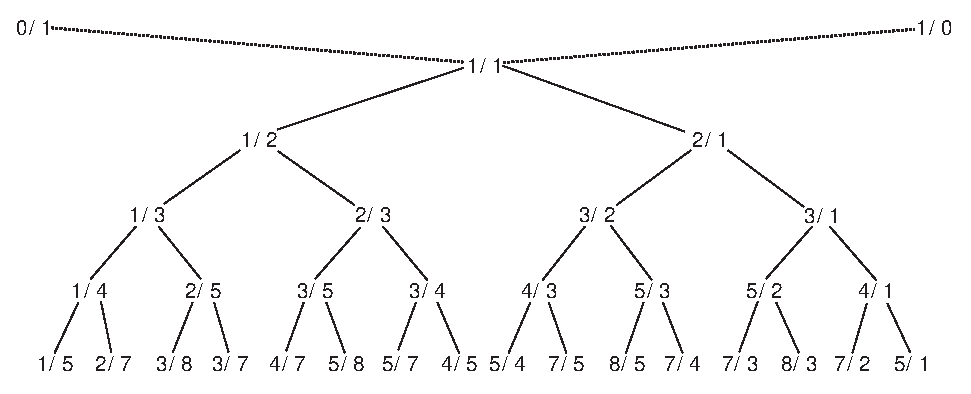
\includegraphics[width=4.6in]{c_cfr0/sbtdpt01.eps}
\caption{The Stern-Brocot Tree}
\label{fig:ccfr0:ssbt0:sdpt0:00}
\end{figure}

To construct the tree, one begins with the two fractions $\frac{0}{1}$
and $\frac{1}{0}$, and forms the mediant (see Definition 
\cfryzeroxrefhyphen{}\ref{def:cfry0:spfs:02})
of two adjacent fractions as many
times as desired to generate additional fractions.
Figure \ref{fig:ccfr0:ssbt0:sdpt0:00} illustrates the construction process.
Note in Figure \ref{fig:ccfr0:ssbt0:sdpt0:00} that the adjacent fractions
are always above and to the left and above and to the right of the fraction
being constructed, and that in the construction of the Stern-Brocot
tree, one of the adjacent fractions can be many levels upwards in the tree
from the fraction being constructed.  For example, in 
Figure \ref{fig:ccfr0:ssbt0:sdpt0:00}, when constructing the fraction 
4/5, the left adjacent fraction (3/4) is nearby in the figure, but 
the right adjacent fraction (1/1) is three levels up to the left and
one level up to the right.  Note when constructing the fraction 4/5 that
its right adjacent fraction is \emph{not} 4/3.

Note that it is also possible to maintain the Stern-Brocot tree as an
ordered list, rather than a tree, starting with the list
$\{0/1, 1/0\}$.  An additional element may be inserted
between any two existing elements in the list by forming their mediant,
and this process may be repeated indefinitely.  Note also that two 
elements $s_L$ and $s_R$ are Farey neighbors to any number $\alpha$
if $s_L < \alpha < s_R$ and the mediant of $s_L$ and $s_R$ has a
denominator larger than the order of the Farey series.  This gives a convenient
procedure for forming best rational approximations using only the Stern-Brocot
tree, as the following example shows.

\begin{vworkexamplestatement}
\label{ex:ccfr0:ssbt0:sdpt0:01}
Find the members of $F_{10}$ which enclose $\pi$.
\end{vworkexamplestatement}
\begin{vworkexampleparsection}{Solution}
By repeatedly calculating mediants, terms can be added to the list 
$\{\frac{0}{1}, \frac{1}{0} \}$ until $\pi$ is enclosed and it is not
possible to generate additional enclosing terms whose denominator does not
exceed 10.  This process is carried out below.

\begin{equation}
\left\{ {\frac{0}{1}, \frac{1}{0} } \right\}, 
\left\{ {\frac{0}{1}, \frac{1}{1}, \frac{1}{0} } \right\}, 
\left\{ {\frac{0}{1}, \frac{1}{1}, \frac{2}{1}, \frac{1}{0} } \right\}, 
\left\{ {\frac{0}{1}, \frac{1}{1}, \frac{2}{1}, \frac{3}{1}, \frac{1}{0} } \right\},
\end{equation}

\begin{equation}
\left\{ {\frac{0}{1}, \frac{1}{1}, \frac{2}{1}, \frac{3}{1}, 
         \frac{4}{1}, \frac{1}{0} } \right\}, 
\left\{ {\frac{0}{1}, \frac{1}{1}, \frac{2}{1}, \frac{3}{1}, \frac{7}{2},
         \frac{4}{1}, \frac{1}{0} } \right\}, 
\left\{ {\frac{0}{1}, \frac{1}{1}, \frac{2}{1}, \frac{3}{1}, \frac{10}{3}, \frac{7}{2},
         \frac{4}{1}, \frac{1}{0} } \right\}, 
\end{equation}

\begin{equation}
\left\{ {\frac{0}{1}, \frac{1}{1}, \frac{2}{1}, 
         \frac{3}{1}, \frac{13}{4}, \frac{10}{3}, \frac{7}{2},
         \frac{4}{1}, \frac{1}{0} } \right\}, 
\left\{ {\frac{0}{1}, \frac{1}{1}, \frac{2}{1}, 
         \frac{3}{1}, \frac{16}{5}, \frac{13}{4}, \frac{10}{3}, \frac{7}{2},
         \frac{4}{1}, \frac{1}{0} } \right\}, 
\end{equation}

\begin{equation}
\left\{ {\frac{0}{1}, \frac{1}{1}, \frac{2}{1}, 
         \frac{3}{1}, \frac{19}{6}, \frac{16}{5}, \frac{13}{4}, \frac{10}{3}, \frac{7}{2},
         \frac{4}{1}, \frac{1}{0} } \right\}, 
\end{equation}

\begin{equation}
\left\{ {\frac{0}{1}, \frac{1}{1}, \frac{2}{1}, 
         \frac{3}{1}, \frac{22}{7}, \frac{19}{6}, 
		 \frac{16}{5}, \frac{13}{4}, \frac{10}{3}, \frac{7}{2},
         \frac{4}{1}, \frac{1}{0} } \right\}, 
\end{equation}

\begin{equation}
\left\{ {\frac{0}{1}, \frac{1}{1}, \frac{2}{1}, 
         \frac{3}{1}, \frac{25}{8}, \frac{22}{7}, \frac{19}{6}, 
		 \frac{16}{5}, \frac{13}{4}, \frac{10}{3}, \frac{7}{2},
         \frac{4}{1}, \frac{1}{0} } \right\}. 
\end{equation}

Note that 25/8 and 22/7 are the left and right neighbors to
$\pi$ in $F_{10}$, since $25/8 < \pi < 22/7$, and since the 
mediant of 25/8 and 22/7 (49/15) has a denominator which is
too large for the Farey series being considered.

Note also that the construction process above could be 
trivially amended to treat the case of a constrained numerator 
rather than a constrained denominator.
\end{vworkexampleparsection}
\vworkexamplefooter{}

The Stern-Brocot tree has many remarkable properties (especially in view of the 
simplicity of its construction).  We mention the following properties
without proof.

\begin{itemize}
\item Each rational number in the tree is irreducible.

\item Each rational number appears in the tree only once.

\item Every positive rational number appears in the tree (i.e. there are no rational
      numbers absent).
\end{itemize}

A more detailed discussion of the Stern-Brocot tree and proof of its
properties is provided
in \cite{bibref:b:concretemathematics}, pp. 116-123.

%%%%%%%%%%%%%%%%%%%%%%%%%%%%%%%%%%%%%%%%%%%%%%%%%%%%%%%%%%%%%%%%%%%%%%%%%%%%%
%%%%%%%%%%%%%%%%%%%%%%%%%%%%%%%%%%%%%%%%%%%%%%%%%%%%%%%%%%%%%%%%%%%%%%%%%%%%%
%%%%%%%%%%%%%%%%%%%%%%%%%%%%%%%%%%%%%%%%%%%%%%%%%%%%%%%%%%%%%%%%%%%%%%%%%%%%%
\subsection{The Correspondence Between The Stern-Brocot Tree And The
            Apparatus Of Continued Fractions}
%Section tag:  DPT0
\label{ccfr0:ssbt0:sdpt1}

The Stern-Brocot tree, on examination, bears a clear resemblence to
the apparatus of continued fractions.  For example, in examining
Figure \ref{fig:ccfr0:ssbt0:sdpt0:00} and following leftmost branches in 
the tree, the rational numbers 1/2, 1/3, 1/4, and 1/5 correspond respectively
to the continued fractions [0;2], [0;3], [0;4], and [0;5].  Similarly,
following 
the right branches down from 1/2 yields, in order, [0;1,2], [0;1,3], and 
[0;1,4].  Clearly, a relationship between the Stern-Brocot tree and the
apparatus of continued fractions may exist.

Suspicions of a simple relationship may also arise by noting that the 
way in which the Stern-Brocot tree is constructed when only left branches
or only right branches are pursued is of the same form as the rule for
the formation of continued fraction convergents (Eqns. 
\ref{eq:thm:ccfr0:scnv0:canonicalconvergentconstruction:01}
and \ref{eq:thm:ccfr0:scnv0:canonicalconvergentconstruction:02}).  For example,
the $n$th successor to the right of 1/3 has the form

\begin{equation}
\label{eq:ccfr0:ssbt0:sdpt1:01}
\frac{n + 1}{2n+3},
\end{equation}

\noindent{}which is suspiciously similar to 
(\ref{eq:thm:ccfr0:scnv0:canonicalconvergentconstruction:01}) and 
(\ref{eq:thm:ccfr0:scnv0:canonicalconvergentconstruction:02}).

There is, in fact, an intimate relationship between the Stern-Brocot
tree and the apparatus of continued fractions.  We present 
this relationship as
Lemma \ref{lem:ccfr0:ssbt0:sdpt1:sbtcfcorrespondence}, 
below.

\begin{vworklemmastatement}
\label{lem:ccfr0:ssbt0:sdpt1:sbtcfcorrespondence}
Let $R^{z_0}L^{z_1} \ldots{} L^{z_{j-2}} R^{z_{j-1}} L^{z_{j}}$ 
or $R^{z_0}L^{z_1} \ldots{} R^{z_{j-2}} L^{z_{j-1}} R^{z_{j}}$
(depending on whether the final leg of the path is towards the
left or towards the right, respectively) be the path in the
Stern-Brocot tree from the fraction 1/1 to the fraction $a/b$, where
$L^N$ denotes traveling downward and to the left in the tree
$N$ nodes, and $R^N$ denotes traveling downward and to the right
in the tree $N$ nodes.  Then the continued fraction representation
of $a/b$ is $[z_0; z_1, \ldots{}, z_{j-2}, z_{j-1}, z_j + 1]$.
\end{vworklemmastatement}
\begin{vworklemmaproof}
The proof is inductive.  First note that the constraints of the path
require that $z_0 \geq 0$, and that $z_k \geq 1$, $k > 0$.  In other
words, only the first rightward leg of the path can have zero steps.

If the path is $R^{z_0}$, $z_0 = 0$, then the lemma predicts that the continued fraction
representation will be $[z_0 + 1]$ = $[1]$, which is the correct continued
fraction representation of the fraction 1/1.  Note that the rational number
1/1 has no ancestor in the tree.

If the path is $R^{z_0}$, $z_0 \neq 0$, then the lemma predicts that the
continued fraction representation will be $[z_0 + 1]$, which is correct
on inspection since the most rightward path in the Stern-Brocot tree
traverses the non-negative integers.  Note that the immediate ancestor of
the fraction $[z_0 + 1]$ is $[z_0]$.

If the path is $R^{z_0}, L^{z_1}$, $z_0 = 0$, then the
fraction $a/b$ will be the weighted mediant of
1/1 and 0/1,

\begin{equation}
\label{eq:ccfr0:ssbt0:sdpt1:02}
\frac{1}{z_1 + 1}
=
[0; z_1 + 1],
\end{equation}

\noindent{}which argrees with the lemma.  Note that the 
immediate ancestor ancestor of $[0; z_1 + 1]$ in the
tree is $[0; z_1]$. 

If the path is $R^{z_0}, L^{z_1}$, $z_0 \neq 0$, then the
fraction $a/b$ will be the weighted mediant of
$(z_0 + 1)/1$ and $z_0/1$, i.e.

\begin{equation}
\label{eq:ccfr0:ssbt0:sdpt1:03}
\frac{(z_0 + 1) + (z_0 z_1)}{(1) + (z_1)}
= z_0 + \frac{1}{z_1 + 1}
= [z_0; z_1 + 1],
\end{equation}

\noindent{}which is consistent with the lemma.  Note also that
the immediate ancestor of the rational number specified by
(\ref{eq:ccfr0:ssbt0:sdpt1:03}) is

\begin{equation}
\label{eq:ccfr0:ssbt0:sdpt1:03b}
\frac{(z_0 + 1) + z_0 (z_1 - 1)}{(1) + (z_1 - 1)}
= z_0 + \frac{1}{z_1}
= [z_0; z_1].
\end{equation}

The cases with two or fewer path components have been
proved above.  It remains to prove all cases with three
or more path components.

Let $s_k = p_k/q_k$ denote the $k$th-ordered convergent
of the continued fraction $[z_0; z_1, \ldots{}, z_{j-1}, z_j]$
(note that the final partial quotient is \emph{not} adjusted upwards by one).
For $k \geq 2$, we can establish a relationship between
$[z_0; z_1, \ldots{}, z_{k-1}, z_k]$
and
$[z_0; z_1, \ldots{}, z_{k-1}, z_k + 1]$ 
as follows:

\begin{equation}
\label{eq:ccfr0:ssbt0:sdpt1:04}
[z_0; z_1, z_2, \ldots{}, z_{k-2}, z_{k-1}, z_k + 1]
=
\frac{(z_k + 1)p_{k-1} + p_{k-2}}{(z_k + 1)q_{k-1} + q_{k-2}}
=
\frac{p_k + p_{k-1}}{q_k + q_{k-1}}.
\end{equation}

If we agree for convenience, as was mentioned in
Section \ref{ccfr0:scnf0}, that we will define $s_{-1} = p_{-1}/q_{-1} = 1/0$, 
then (\ref{eq:ccfr0:ssbt0:sdpt1:04}) holds for $k \geq 1$.

\textbf{(Inductive Step):} Assume that the lemma holds
up through $k-1$.  For a path in the Stern-Brocot tree
$R^{z_0}L^{z_1} \ldots{} L^{z_{k-2}} R^{z_{k-1}} L^{z_{k}}$ 
or $R^{z_0}L^{z_1} \ldots{} R^{z_{k-2}} L^{z_{k-1}} R^{z_{k}}$, 
$k \geq 2$, the ``reversal'' fraction above (i.e. the fraction where the path changes
directions) is

\begin{equation}
\label{eq:ccfr0:ssbt0:sdpt1:05}
[z_0; \ldots{}, z_{k-2}, z_{k-1} + 1] = 
\frac{p_{k-1} + p_{k-2}}{q_{k-1} + q_{k-2}}
\end{equation}

\noindent{}(this is established by the lemma on the path through $k-1$ and by
Eqn. \ref{eq:ccfr0:ssbt0:sdpt1:04}).

The immediate ancestor of the fraction specified in 
(\ref{eq:ccfr0:ssbt0:sdpt1:05}) is

\begin{equation}
\label{eq:ccfr0:ssbt0:sdpt1:06}
[z_0; \ldots{}, z_{k-2}, z_{k-1}] = 
\frac{z_{k-1}p_{k-2} + p_{k-3}}{z_{k-1}q_{k-2} + q_{k-3}} ,
\end{equation}

\noindent{}as was shown to hold in (\ref{eq:ccfr0:ssbt0:sdpt1:03b}) and
in the inductive step.

The rational number corresponding to the path
$R^{z_0}L^{z_1} \ldots{} L^{z_{k-2}} R^{z_{k-1}} L^{z_{k}}$ 
or $R^{z_0}L^{z_1} \ldots{} R^{z_{k-2}} L^{z_{k-1}} R^{z_{k}}$
is a weighted mediant of (\ref{eq:ccfr0:ssbt0:sdpt1:05}) 
and (\ref{eq:ccfr0:ssbt0:sdpt1:06}):

\begin{eqnarray}
\label{eq:ccfr0:ssbt0:sdpt1:07}
\hspace{-0.35in}
\frac{z_k(z_{k-1}p_{k-2} + p_{k-3}) + p_{k-1} + p_{k-2}}
     {z_k(z_{k-1}q_{k-2} + q_{k-3}) + q_{k-1} + q_{k-2}}
 & = &
\frac{(z_k + 1)p_{k-1} + p_{k-2}}{(z_k + 1)q_{k-1} + q_{k-2}} \\
\label{eq:ccfr0:ssbt0:sdpt1:08}
& = & \frac{p_k + p_{k-1}}{q_k + q_{k-1}} \\
& = & [z_0; z_1, \ldots{}, z_{k-1}, z_{k} + 1],
\end{eqnarray}

\noindent{}which establishes the main result of the lemma in the
inductive step.  Note also that the immediate ancestor of the
fraction specified in (\ref{eq:ccfr0:ssbt0:sdpt1:07}) is 
$[z_0; \ldots{}, z_{k-1}, z_{k}]$ (which is necessary for 
the inductive step).  This proves the lemma.
\end{vworklemmaproof}
\begin{vworklemmaparsection}{Remarks}
This lemma provides a straightforward method to go from a
fraction's position in the Stern-Brocot tree to its continued
fraction representation, or vice-versa.

To go from a fraction's position in the Stern-Brocot tree to its
continued fraction representation:

\begin{itemize}
\item Starting with moves downward and to the right from the
      fraction 1/1 ($z_0$), observe the length of the alternating
      rightward and leftward node traversals required to reach
	  the desired fraction.

\item Adjust the final length upward by one.

\item These lengths in order are then the successive partial quotients
      of the fraction.
\end{itemize}

To go from the continued fraction representation of a fraction
to its position in the Stern-Brocot tree:

\begin{itemize}
\item Reduce the final partial quotient by one.

\item Use the partial quotients, in order, in an alternating fashion,
      to go rightward and downward
      and leftward and downward in the Stern-Brocot tree.  The fraction
	  reached on the final leg will be the fraction of interest.
\end{itemize}
\end{vworklemmaparsection}
\vworklemmafooter{}

It is clear from the lemma above that the Stern-Brocot tree and the 
apparatus of continued fractions are intimately related.  Specifically,
the Stern-Brocot tree provides a model for the formation and arrangement
of rational numbers, but the apparatus of continued fractions provides
a much more efficient way to navigate the Stern-Brocot tree and to find
best rational approximations.

%%%%%%%%%%%%%%%%%%%%%%%%%%%%%%%%%%%%%%%%%%%%%%%%%%%%%%%%%%%%%%%%%%%%%%%%%%%%%
%%%%%%%%%%%%%%%%%%%%%%%%%%%%%%%%%%%%%%%%%%%%%%%%%%%%%%%%%%%%%%%%%%%%%%%%%%%%%
%%%%%%%%%%%%%%%%%%%%%%%%%%%%%%%%%%%%%%%%%%%%%%%%%%%%%%%%%%%%%%%%%%%%%%%%%%%%%
\subsection{Using The Stern-Brocot Tree To Find Best Rational Approximations}
%Section tag:  USB0
\label{ccfr0:ssbt0:susb0}

It is clear from Example \ref{ex:ccfr0:ssbt0:sdpt0:01} that the Stern-Brocot
tree can be used to find best rational approximations in the Farey series
of any order, simply by forming mediants until the number of interest
is enclosed.  It is also clear that an algorithm of repeatedly forming
mediants in order to find a best rational approximation in
$F_{k_{MAX}, \overline{h_{MAX}}}$ can be devised.

However, the sole drawback of such a procedure is that building the Stern-Brocot
tree from the top in order to find neighbors in $F_N$ is an
$O(N)$ procedure, which renders it unsuitable for use with large
$N$.  For this reason, the continued fraction algorithms presented
earlier in the chapter, which are $O(log \; N)$ (due to the 
guaranteed minimum exponential rate of increase of convergent
denominators, Theorem \ref{thm:ccfr0:scnv0:minimumrateofconvergentdenominatorincrease}),
are the only practical algorithms.


%%%%%%%%%%%%%%%%%%%%%%%%%%%%%%%%%%%%%%%%%%%%%%%%%%%%%%%%%%%%%%%%%%%%%%%%%%%%%
%%%%%%%%%%%%%%%%%%%%%%%%%%%%%%%%%%%%%%%%%%%%%%%%%%%%%%%%%%%%%%%%%%%%%%%%%%%%%
%%%%%%%%%%%%%%%%%%%%%%%%%%%%%%%%%%%%%%%%%%%%%%%%%%%%%%%%%%%%%%%%%%%%%%%%%%%%%
\section{Practical Techniques}
%Section tag:  PTQ0

Although this chapter has presented rather theoretical results and techniques
from number theory, our emphasis is on practical applications (which is why
we've concentrated on finding Farey neighbors of \emph{rational} numbers).
Practicing engineers would be more likely to use the digits from a calculator
as the starting point to obtain a rational approximation than to use 
a symbolic irrational constant, such as $\pi$.

In this section, we present \emph{practical} techniques---those most likely
to be used in practice by microcontroller software developers.



%%%%%%%%%%%%%%%%%%%%%%%%%%%%%%%%%%%%%%%%%%%%%%%%%%%%%%%%%%%%%%%%%%%%%%%%%%%%%
%%%%%%%%%%%%%%%%%%%%%%%%%%%%%%%%%%%%%%%%%%%%%%%%%%%%%%%%%%%%%%%%%%%%%%%%%%%%%
%%%%%%%%%%%%%%%%%%%%%%%%%%%%%%%%%%%%%%%%%%%%%%%%%%%%%%%%%%%%%%%%%%%%%%%%%%%%%
\subsection{Practical Aspects Of Beginning With A Rational Approximation}
%Subsection tag:  PAS0
\label{ccfr0:sptq0:sspas0}

In practical applications, one often begins with a rational approximation 
to a irrational number.  
For example, one might use 3.14159265359 (from
a calculator) as the value of $\pi$ for the application of 
Algorithm \ref{alg:ccfr0:scrn0:akgenalg}.  This naturally raises the
question of how accurate the rational approximation used
as a starting point must be to avoid identifying the wrong 
rational numbers as Farey neighbors.  We illustrate the possibility
of identifying the wrong rational number with an example.

\begin{vworkexamplestatement}
\label{ex:ccfr0:sptq0:01}
Find the members of $F_{255}$ which enclose $\pi$, using 
3.1416 as the value of $\pi$.
\end{vworkexamplestatement}
\begin{vworkexampleparsection}{[Erroneous] Solution And Remarks}
It can be shown using the methods presented earlier that
the members of $F_{255}$ which enclose 3.1416 are
355/113 and 732/333, i.e.

\begin{equation}
\frac{355}{113} < 3.1416 < \frac{732}{333} .
\end{equation}

However, in fact, 688/219 and 355/113 are the actual enclosing
neighbors of $\pi$ in $F_{255}$:

\begin{equation}
\frac{688}{219} < \pi < \frac{355}{113} < 3.1416 < \frac{732}{333} .
\end{equation}

Thus by using an imprecise approximation of $\pi$, we have incorrectly
identified the neighbors to $\pi$ in $F_{255}$.
\end{vworkexampleparsection}
\vworkexamplefooter{}

How do we avoid incorrectly identifying the rational
numbers which enclose an irrational number when a
rational approximation of the irrational number is
used as the starting point for the selection algorithm?
There are three practical approaches to the problem.

Observe that when we know
the first several decimal digits of an irrational number,
the actual value of the irrational number is confined
to an interval.  For example, if a calculator displays
``3.1416'' as the value of $\pi$, we might safely
assume that $3.14155 \leq \pi \leq 3.14165$, if the
digits that the calculator displays were 
obtained by rounding.  

As a first approach to dealing with a rational approximation
to an irrational number,
we might simply determine the
Farey neighbors of both endpoints of the interval of
uncertainty.  For example, if
314,155/100,000 and 314,165/100,000 have the same 
Farey neighbors in a Farey series of interest (which we can
easily determine using the algorithms presented earlier
in this chapter), we could
correctly deduce that these Farey neighbors are the
Farey neighbors of $\pi$.  On the other hand,
if 314,155/100,000 and 314,165/100,000 have different
enclosing Farey neighbors, then there are Farey 
terms in the interval [3.14155, 3.14165],
and more information about $\pi$
would be required to determine its true Farey neighbors.

A second approach to this same problem would be to devise an
algorithm to process
the endpoints of the interval of uncertainty simultaneously and note
when their partial quotients diverge.  

A third approach, which is 
perhaps the most direct, is to apply 
Algorithm \cfryzeroxrefhyphen{}\ref{alg:cfmindenominator} to determine
the rational number with the minimum denominator in the interval of uncertainty.
We would thus know that we have enough information to determine uniquely the
enclosing rational numbers in any Farey series up to one less than this 
minimum denominator.

\begin{vworkexamplestatement}
\label{ex:ccfr0:sptq0:02}
Assume that 3.142 is the only value for $\pi$ available.  What is the maximum
order of the Farey series where the enclosing rational numbers to $\pi$ can
be unambiguously determined?
\end{vworkexamplestatement}
\begin{vworkexampleparsection}{Solution}
Assume that the constant ``3.142'' was obtained by rounding of digits, rather than
by truncation of digits:  thus $3.1415 \leq \pi \leq 3.1425$.  Applying
Algorithm \cfryzeroxrefhyphen{}\ref{alg:cfmindenominator} yields 333/106
as the rational number with the smallest denominator in the interval
[3.1415, 3.1425].  Thus, no rational number with a smaller denominator exists
in the interval, and the enclosing rational numbers of $\pi$ in the Farey series of
up to order 105 can be determined with the limited information available.
\end{vworkexampleparsection}
\vworkexamplefooter{}


%%%%%%%%%%%%%%%%%%%%%%%%%%%%%%%%%%%%%%%%%%%%%%%%%%%%%%%%%%%%%%%%%%%%%%%%%%%%%
%%%%%%%%%%%%%%%%%%%%%%%%%%%%%%%%%%%%%%%%%%%%%%%%%%%%%%%%%%%%%%%%%%%%%%%%%%%%%
%%%%%%%%%%%%%%%%%%%%%%%%%%%%%%%%%%%%%%%%%%%%%%%%%%%%%%%%%%%%%%%%%%%%%%%%%%%%%
\subsection{Obtaining Irrational Numbers To High Precision}
%Subsection tag:  OIN0
\label{ccfr0:sptq0:ssoin0}

It may happen in practice that one desires more information about an
irrational number than can be easily obtained.  As a practical example,
a typical scientific calculator treats $\pi$ as 3.14159265359, implying that 
$3.141592653585 \leq \pi \leq 3.141592653595$.  Application of 
Algorithm \cfryzeroxrefhyphen{}\ref{alg:cfmindenominator} to this
interval yields 1,146,408/364,913 as the rational number with the
smallest denominator in this interval:  implying that we cannot determine the 
enclosing rational approximations to $\pi$ even in $F_{2^{32}-1}$ using
the information most readily available.  How do we obtain more digits of $\pi$?
And even if we can obtain more digits of $\pi$, how do we manipulate rational
numbers with such large integer components?  (We discuss the problem of obtaining
more digits below, but discuss manipulation in Section \ref{ccfr0:sptq0:smhp0}.)

There are two approaches to determining $\pi$ or other numbers to
high precision.

\begin{enumerate}

\item Locate information about the number on the Web or in a reference
      book.  (Note that decimal digits of the number, partial quotients
	  of the number, or convergents of the number can all be used; and it
	  is typical for all of these to be somewhere on the Web.  However,
	  convergents are the most useful form for obtaining best rational
	  approximations.)

\item Use commercial symbolic manipulation software (\index{Mathematica@\emph{Mathematica}}\emph{Mathematica}
      \cite{bibref:s:wolframmathematica}, 
      for example) to
      obtain the number of interest to arbitrary 
      precison.\footnote{\label{footnote:ccfr0:sptq0:ssoin0:mathematicaexpensive}\emph{Mathematica}
      \cite{bibref:s:wolframmathematica} is quite expensive (version 4.1 
      for Windows, as of March 2001, is \$1,495), 
      and something that a microcontroller software developer
      would very rarely use, so we assume that most microcontroller software
      developers would search for a less expensive solution.}

\end{enumerate}

%%%%%%%%%%%%%%%%%%%%%%%%%%%%%%%%%%%%%%%%%%%%%%%%%%%%%%%%%%%%%%%%%%%%%%%%%%%%%
%%%%%%%%%%%%%%%%%%%%%%%%%%%%%%%%%%%%%%%%%%%%%%%%%%%%%%%%%%%%%%%%%%%%%%%%%%%%%
%%%%%%%%%%%%%%%%%%%%%%%%%%%%%%%%%%%%%%%%%%%%%%%%%%%%%%%%%%%%%%%%%%%%%%%%%%%%%
\subsection{Manipulating High-Precision Rational Numbers}
%Subsection tag:  MHP0
\label{ccfr0:sptq0:smhp0}

Assuming that one is able to determine a [rational or irrational] number
of interest to high-precision (either a large number of decimal digits or a rational
number with large integer components), how does
one manipulate rational numbers with large integer components?
In this section, we list software alternatives.

The first alternative we should mention is \emph{The Iju Tool Set}, distributed
with this book.  Starting with version 1.05, this tool set contains
a subset of the GNU MP Library \cite{bibref:s:gnumultipleprecisionarithmeticlibrary}, 
and will manipulate 
large integers and rational numbers with large integer components.  To provide
more flexibility for the user, this tool set is embedded as extensions to
the Tcl scripting language; so that any of the functionality provided can be
used either interactively or from within a Tcl script.

\begin{figure}
\centering
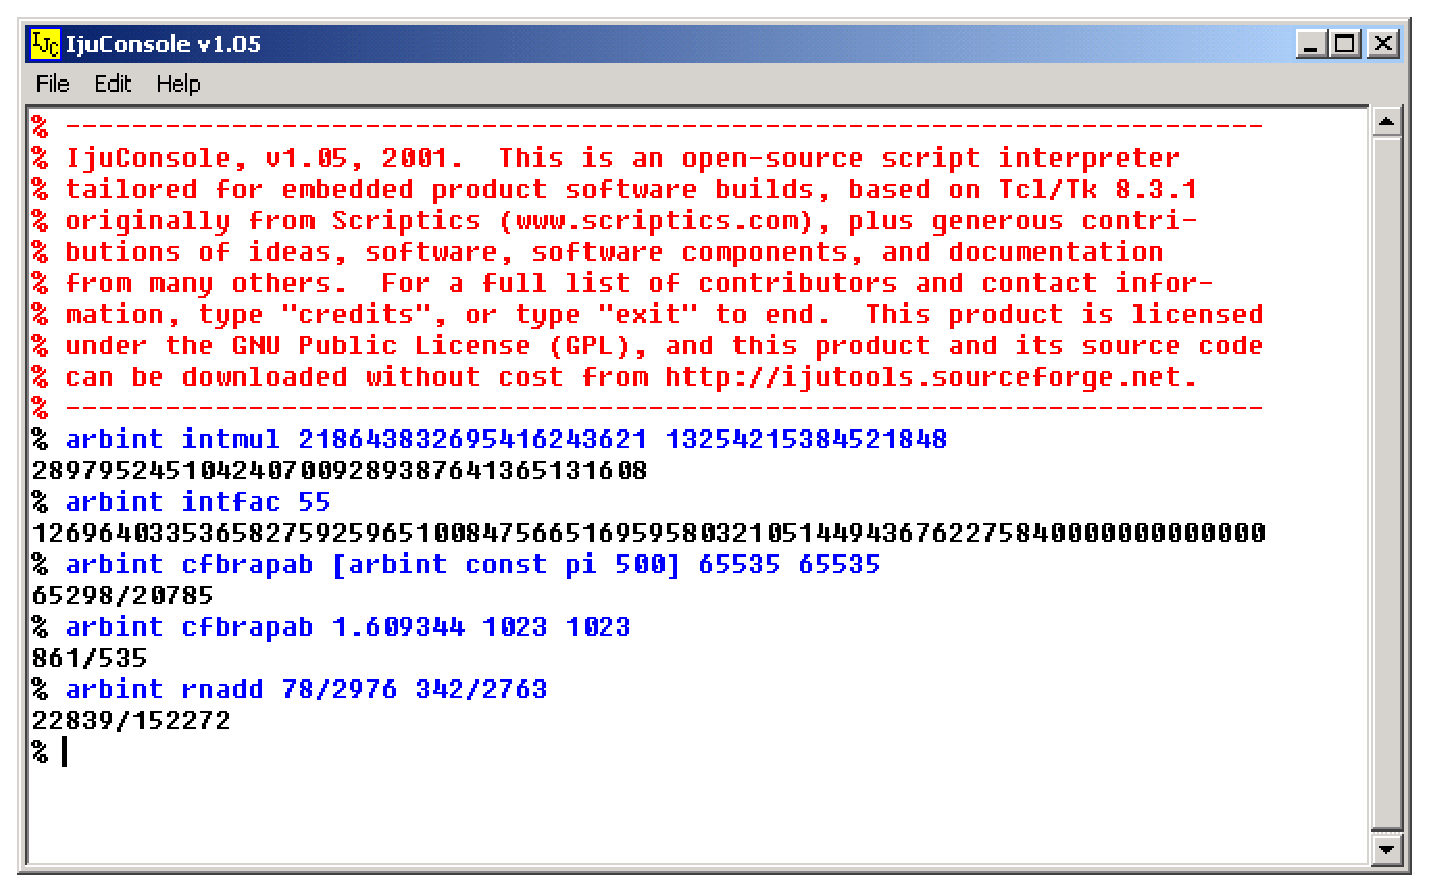
\includegraphics[width=4.6in]{c_cfr0/ijt_ss01.eps}
\caption{Large Integer Arithmetic And Best Rational Approximations Using \emph{IjuConsole}
         From \emph{The Iju Tool Set}}
\label{fig:ccfr0:sptq0:smhp0:00}
\end{figure}

Figure \ref{fig:ccfr0:sptq0:smhp0:00} shows a screen snapshot\footnote{By
the way, \emph{IjuConsole} will handle \emph{much} larger integers, but 
small examples were used so that all of the information would fit
in a single screen snapshot.} of
\emph{IjuConsole} (the \emph{Wish}-like Tcl
interpreter from \emph{The Iju Tool Set}) being used interactively
to provide the answers to several questions involving large integers and
rational numbers with large integer components.  The first command
shown,\\

\texttt{arbint intmul 218643832695416243621 13254215384521848},\\

\noindent{}illustrates integer multiplication.  The second command shown,\\

\texttt{arbint intfac 55},\\ 

\noindent{}illustrates calculating the factorial of
55.  The third command shown, \\

\texttt{arbint cfbrapab [arbint const pi 500] 65535 65535},\\

\noindent{}illustrates calculating the best rational approximation to 
$\pi$ with numerator and denominator not exceeding 
65,535, and using the first 500 digits of $\pi$ as
the value of $\pi$.  The fourth command shown,\\

\texttt{arbint cfbrapab 1.609344 1023 1023},\\

\noindent{}illustrates finding the best rational approximation to 
the conversion factor from MPH to KPH with numerator and denominator
not exceeding 1,023.  The last command shown,\\

\texttt{arbint rnadd 78/2976 342/2763},\\

\noindent{}illustrates the addition of
two rational numbers.

Many other potential solutions for dealing with large
integers have been submitted by newsgroup
posters, and are listed below.  (Please note that these alternatives haven't actually been
tried, and we can't say whether they are viable.)

\begin{enumerate}

\item \index{Mathematica@\emph{Mathematica}}\emph{Mathematica} 
      \cite{bibref:s:wolframmathematica} (by Wolfram Research) will easily operate on large integers and 
      rational numbers with large integer components  (see
      Footnote \ref{footnote:ccfr0:sptq0:ssoin0:mathematicaexpensive}).
      (Suggested by \index{Lutus, Paul} Paul Lutus \cite{bibref:i:paullutus} and
      \index{Taylor, Don} Don Taylor \cite{bibref:i:dontaylor}.)

\item \index{GNU!Multiple Precision Arithmetic Library (GMP)}The 
      \emph{GNU Multiple Precision Arithmetic 
      Library (GMP)} \cite{bibref:s:gnumultipleprecisionarithmeticlibrary}.
      This library, which is free and on the Web, can be linked into
      `C' and `C++' programs, and allows fast integer calculations of
      any size that do not exceed the memory available in the computer.
      This library could be used to quickly construct a program to 
      process rational numbers with very large integer components.

\item \index{UBASIC@\emph{UBASIC}}\emph{UBASIC} \cite{bibref:s:ubasic} 
      (\index{Kida, Yuji}by Yuji Kida \cite{bibref:i:yujikida})
      is an extended-precision version of the BASIC
      language which will handle integers up to 2,600 digits and
      exact rational arithmetic. (Suggested by \index{Schorn, Richard} Richard Schorn 
      \cite{bibref:i:richardschorn}.)

\item \index{Derive 5@\emph{Derive 5}}\emph{Derive 5} \cite{bibref:s:derive5} (by Texas Instruments).
      The exact capabilities of this software are not known, but the Web page indicates
      it can perform exact rational arithmetic.  (Suggested by \index{Schorn, Richard} Richard Schorn 
      \cite{bibref:i:richardschorn} and \index{Taylor, Don} Don Taylor \cite{bibref:i:dontaylor}.)

\item \index{Maple@\emph{Maple}}\emph{Maple} \cite{bibref:s:maple} (by Waterloo
      Maple, Inc.).  The exact capabilities of this software are not known.
      (Suggested by 
      \index{Lutus, Paul} Paul Lutus \cite{bibref:i:paullutus} and
      \index{Taylor, Don} Don Taylor \cite{bibref:i:dontaylor}.)

\item \index{MuPAD@\emph{MuPAD}}\emph{MuPAD} \cite{bibref:s:mupad} (from
      the University Of Paderborn, Germany).  The capabilities of this
      software are not known.  (Suggested by \index{Schorn, Richard} Richard Schorn 
      \cite{bibref:i:richardschorn}.)

\end{enumerate}

%http://www.csc.fi/math_topics/Mail/FAQ/msg00015.html

In addition to the large integer resources above, a 
much longer list of resources is maintained
at the URL

\begin{quote}
\texttt{http://www.csc.fi/math\_topics/Mail/FAQ/msg00015.html},
\end{quote}

\noindent{}and is reproduced below.  Because this URL was apparently last updated
in 1994, it is not known which of the resources listed are still
available.

\begin{quote}
\begin{scriptsize}
\begin{verbatim}
--------------------------------------------------------------------------------
Subject: List of Arbitrary Precision C packages 
From: mrr@scss3.cl.msu.edu (Mark Riordan) 
Date: 27 Jan 1994 16:06:01 GMT 
Newsgroups: sci.math 
--------------------------------------------------------------------------------
This is the file BIGNUMS.TXT from ripem.msu.edu, last updated January 1994.

In response to Email requests, I have assembled this list of
large-integer arithmetic packages of which I have heard.
Most of these are C function libraries, available in source form.
A few also deal with floating point numbers.  

For your convenience, I have placed copies of
some of these on ripem.msu.edu (35.8.1.178).  They are
available for anonymous FTP in the directory "pub/bignum".
However, what I have may not be the most current version in all cases.

Here they are, in no particular order:

mp
    Multiple Precision package that comes with some Unixes
    
    Multiple precision package accessed via -lmp flag on your
    compiler.  Provides +, -, *, /, gcd, exponentiation,
    sqrt.  Comes with SunOS, NeXT Mach, BBN Mach 1000, 
    and probably a few others.  See "man 3 mp".  
    Object code only, of course.

PARI
    Henri Cohen, et al., Universite Bordeaux I, Paris, FRANCE
    
    Multiple precision desk calculator and library routines.
    Contains optimized assembly code for Motorola 68020, 
    semi-optimized code for SPARC, and apparently rather slow
    generic C version.  Does both integers and reals.
    Does vectors and matrices as well as scalars.
    Contains a number of advanced functions, some of which I've
    never heard of.  ("Weber's function"?)
    Has a factorization function, primality test, & other related stuff.
    Plenty of TEX documentation.
    Public domain, but you can't distribute modified versions.
    Available via anonymous FTP from ftp.inria.fr:lang/ and 
    math.ucla.edu.  The ucla site has Mac, MSDOS, OS/2, and
    NeXT-specific versions there in addition to:
    Filename:  pari-1.37.tar.Z  (There are now more recent versions)
    
Arithmetic in Global Fields  (Arith)
    Kevin R. Coombes, David R. Grant
    
    Package of routines for arbitrary precision integers or
    polynomials over finite fields.  Includes basic +, -, *, /
    and a few others like gcd.  Source code in C.
    Distributed under the terms of the GNU public license.
    Includes man pages and TEX documentation.
    Filename:  arith.tar.Z

Arbitrary Precision Math Library
    Lloyd Zusman   Los Gatos, CA
    
    C package which supports basic +, -, *, /.  Provides for radix
    points (i.e., non-integers).  Not as polished as the others here.
    Posted to comp.sources.misc in October 1988.
    Filename:  apml.tar.Z
    
BigNum
    J. Vuillemin, INRIA, FRANCE, and others.
    Distributed by Digital Equipment Paris Research Lab (DECPRL)
    
    A "portable and efficient arbitrary-precision integer" package.
    C code, with generic C "kernel", plus assembly "kernels" for
    MC680x0, Intel i960, MIPS, NS32032, Pyramid, and of course VAX.
    This is probably one of the better-known packages of this type.
    Implements +, -, *, /, mod, plus logical operations OR, AND, XOR.
    Both signed and unsigned arithmetic available.
    Available via email from librarian@decprl.dec.com.
    You will receive 5 shell archives.  Give your postal address
    and you will also receive printed documentation from France.
    Package includes TEX documentation.
    Publicly available for non-commercial use.
    I removed this from my archive when I heard a rumor that PRL
    doesn't like others to distribute it.  However, BIGNUM *is*
    distributed as part of ecpp (see below).

Lenstra's LIP package
    Arjen Lenstra   Bellcore
    
    Portable unsigned integer package written entirely in C.
    Includes +, -, *, /, exponentiation, mod, primality testing,
    sqrt, random number generator, and a few others.  
    An earlier version of this package is the only of these packages
    I have actually used.  It works well and is very portable.  
    I haven't done any benchmarks against the others, but the code 
    looks clever & Lenstra is an accomplished number theorist.

    LIP replaces lenstra-3.1.c.  The package now includes encrypted
    source code; to obtain the decryption key, you must send a
    signed license agreement to Bellcore.  See the documentation.
    Filename:  lenstra-LIP-package.tar  This is a collection of
    all the files in flash.bellcore.com:/pub/lenstra

bmp  (Brent's Multiple Precision?)
    R. P. Brent

    1981 vintage FORTRAN code to do extended precision floating &
    fixed point arithmetic.  Includes most of the mathematical
    functions you'd find in a FORTRAN run-time library.
    This code is an ACM algorithm, number 524.
    To obtain, send a mail message to  netlib@ornl.gov
    containing the line "send mp.f from bmp" or better yet, perhaps
    just start with "help".

SPX
    Kannan Alagappan & Joseph Tardo, DEC
    
    This is a huge prototype public key authentication system
    based on RSA.  I mention it here because those who have heard
    of SPX have probably correctly guessed that it contains a large
    integer package and I want to inform you that the large integer
    package it contains is indeed DEC's BigNum from France.
    You can get a beta test copy of SPX from crl.dec.com (192.58.206.2). 
    Use it only for testing, as it "may" expire on a certain date.
    (I don't know whether this has expired yet.)

amp  (Antti's Multiple Precision?)
    Antti Louko   alo@kampi.hut.fi

    Multiple precision integer package in C.  Includes +, -, *, /, %,
    pow, mod, 1/x mod y, random, sqrt, gcd.  Available for non-commercial
    use.  The package includes "share-secret", a public key system based
    on the Diffie-Hellman algorithm.
    This is normally part of the well-known "des-dist.tar.Z",
    but I have removed the DES part to avoid having to deal with 
    cryptographic export laws, and have named the result:
    Filename:  amp.tar.Z

gennum  
    Per Bothner   U of Wisconsin-Madison

    C++ routines and classes to do generic arithmetic, both
    integer and rational.  Part of the "Q" programming system.
    Distributed under the terms of the GNU public license.
    Obtained from cygnus.com.
    Filename: gennum.tar.Z

MIRACL
    (Shamus Software, Dublin, Ireland)

    Integer and fractional multiple precision package.
    MIRACL is a portable C library. Full C/C++ source code included 
    (In-line assembly support for 80x86). Number theoretic primitives
    needed to support PK Cryptography are supplied.   
    C++ classes for Multiprecision Integers, Modular arithmetic, and 
    Chinese Remainder Thereom. Implementation in C/C++ of all modern 
    methods of Integer Factorisation, viz Brent-pollard, p-1, p+1, 
    Elliptic Curve, MPQS.  Includes TEX manual and some DOS .EXEs.
    Not public domain, but free for academic and non-commercial use.
    Obtained from ftp.compapp.dcu.ie.
    Filename:  /pub/crypt/other/miracl-3.23.zip and miracl.tar.Z (older)

precision
    Dave Barrett  barrettd@tigger.colorado.edu

    Multiple precision integer package in C with +,-,*,/, sqrt, rand,
    mod, pow, log.  Simple vector support.  Does dynamic allocation of memory.
    Free as long as you don't sell it or any program that uses it.
    Filename:  precision.tar.Z

UBASIC
    Prof. Yuji Kida, Rikkyo University, Nishi-Ikebukuro 3, Tokyo 171, Japan
    kida@rkmath.rikkyo.ac.jp

    Multiple-precision version of the BASIC programming language,
    for MS-DOS.  Includes floating point.  Said (by Keith Briggs)
    to be pretty fast.  Object only, I think.  ervin@morekypr.bitnet
    says:  "This is the best package that I know of for
    fast arithmetic.  Has a version optimized for 386 machines.  Includes
    routines to do MPQS, the fastest currently known general factoring
    algorithm.  An additional file is at both sites to allow MPQS to use
    hard drives so that it can factor up to 80 digits.  Many number
    theoretical functions are included in UBASIC.  It allows over 2500
    digits of precision."
    Available via anonymous FTP from shape.mps.ohio-state.edu,
    or simtel20.army.mil, or wuarchive.wustl.edu.

calc_v22
    Unknown

    MS-DOS C-like language that allows "infinite" precision.
    Nice intrinsic functions.  ervin@morekypr.bitnet reports problems
    when changing precision on the fly.
    See simtel20 or wuarchive.

briggs_arith
    Keith Briggs (kbriggs@maths.adelaide.edu.au)

    Turbo Pascal 5 source for routines that do multiple-precision
    +, -, *, /, sqrt, gcd, factoring, rand for integers; also includes
    +, -, *, / and rand for rational numbers.
    Filename:  briggs_arith.pas

Institute fur Experimentelle Mathematik
    Dr Gerhard Schneider (?)

    Fast C multiple-precision subroutine library.
    I don't know anything about it; sl25@ely.cl.cam.ac.uk says
    to contact MAT420@DE0HRZ1A.BITNET for more info.
    Postal Address:
    Institute fur Experimentelle Mathematik
    EllernStr 29
    D4300 Essen-12    GERMANY

LongInt
    Markus Mueller (mueller@komsys.tik.ethz.ch)

    "Multi precision arithmetic written in MODULA-2, with the most time critical
    parts written in Assembler. Includes basic arithmetics (+, -, *, /, %) as
    well as arithmetics MODULO a number. An additional module provides a
    collection of procedures for primality testing, gcd, multiplicative
    inverse and more. The package is part of a Privacy Enhanced Mail (PEM)
    package which includes a PEM mailer, RSA key generator and Certificate
    generation tools."

    Source is in Modula-2, C, and assembler for Sun 3.  LongInt has
    also been ported to MS-DOS under Logitech Modula-2 and Turbo
    Assembler.  Availability:  free for university use (research and
    education); otherwise, a source license is required.  To obtain,
    write or email to:

        Markus Mueller
        Bertastrasse 7
        CH-8953 Dietikon
        Switzerland
        email:  mueller@komsys.tik.ethz.ch

bignum-1.2
    Henrik.Johansson@Nexus.Comm.SE

    Bignum package written in portable C.  Will in the future
    conform to the Common Lisp functions that handles integers.
    Currently includes +, -, *, /, exponentiation, "exptmod",
    comparison, random numbers, and gcd.
    Filename: bignum-1.2

ACM algorithm 567
    D.W. LOZIER and J.M. SMITH

    FORTRAN subroutines to do extended-precision floating point
    and normalized Legendre polynomials.
    ACM TRANSACTIONS ON MATHEMATICAL SOFTWARE 7,1 (MARCH, 1981)
    Obtained from research.att.com:netlib/toms/567.Z
    Filename: acm-algorithm-567-floating-point.fortran.Z

range
    O. Aberth and M. J. Schaefer

    C++ package to do extended-precision floating point arithmetic
    with programmer-defined precision.  Uses decimal representations
    internally.  Contains basic +, -, *, /, relational operators,
    ++, and a few functions like sin, cos, sqrt, log.  Documentation
    a trifle confusing.
    Obtained from math.tamu.edu:pub/range/range.tar.Z
    Filename: range.tar.Z

bsint
    Author unknown.

    Pre-alpha release of C++ big integer package.  
    Implements basic math operators, exponentiation, and modular 
    exponentiation.  Very skimpy documentation.
    See milton.u.washington.edu:/pub/user-supported/tzs/bsint.tar.Z

GNU Multiple Precision (GMP)
    GNU (Free Software Foundation) multiple precision package.
    I haven't looked at it yet.  This is current as of April 1992,
    but there may be a more recent version by the time you read 
    this.  This package is very widely available on FTP sites.
    Filename: gmp-1.3.2.tar.Z

libg++ - GNU's C++ class library
    Free Software Foundation

    Includes Integer and Rational classes.  Integer provides
    the usual C++ operators, plus exponentiation, gcd, lcm.
    Limited functionality, but documentation is better than most.
    Look for libg++-2.4.tar.gz on an FTP server near you.

Elliptic Curve Primality Proving 
    Francois Morain, France.

    Large package to prove the primality of any prime.
    Includes Inria's BIGNUM package. 
    Obtained from ftp.inria.fr (128.93.1.26).
    Filename: ecpp.V3.4.1.tar.Z

PGP (Pretty Good Privacy)
    Philip Zimmermann   prz@sage.cgd.ucar.EDU

    Crypto package that includes bignum routines in C.
    Assembly implementations available for several processors;
    said to be quite fast for numbers around 1000 bits in size.
    The crypto package violates RSA patents, but the bignum routines
    can be used without fear of legal repercussions.

Bell's Arbitrary Precision Calculator
    David I. Bell, Australia  (dbell@pdact.pd.necisa.oz.au)

    Arbitrary-precision calculator with good online help, C-like
    language, many builtin functions, support for integers,
    rational numbers (they work like floating point), complex numbers,
    matrices, strings, lists, files, "objects".  Includes 
    gcd, primality testing, even trig functions.  Recommended.
    (Large package, though.)  Obtained from comp.sources.unix.
    Filename: calc-1.24.7.tar.Z

Calc for GNU Emacs
    Dave Gillespie  (daveg@synaptics.com)
   
    Advanced calculator written in Emacs Lisp.  Includes arbitrary
    precision integers and floating point, bitwise operations,
    log and trig functions, financial functions, number theoretic
    functions including prime factorization, symbolic calculus,
    and an interface to GNUPLOT.
    Filename:  calc-2.02a.tar.Z

MPFUN: A Multiple Precision Floating Point Computation Package
    David H. Bailey   (dbailey@nas.nasa.gov)

    Package of Fortran subroutines to perform multiprecision
    floating point arithmetic.  Also includes a program that
    can automatically convert ordinary Fortran-77 code into code
    that calls the MPFUN routines.  
    Keith Briggs says: "It's a masterpiece, and the state of the art 
    as far as Fortran goes."
    Documentation in TeX format.  Unrestricted distribution
    allowed at no cost.
    Filenames: mpfun_fortran.tar.Z & mpfun_tex_papers.tar.Z

MPQS
    Mark S. Manasse  (msm@src.dec.com)  and Arjen Lenstra

    C program to factor numbers on a distributed network of
    heterogeneous machines.  June 1993 version.
    Filename:  mpqs-distributed-factoring.shar

GNU bc
   Author: Philip A. Nelson (phil@cs.wwu.edu)
   GNU bc is an interactive algebraic language with arbitrary precision.
   GNU bc is almost the same as bc & dc in some Unixes.
   Filename: bc-1.02.tar.z  (for example, in GNU prep.ai.mit.edu:pub/gnu/)

bc & dc
  bc is an interactive processor for an arbitrary precision arithmetic
  language or just compiler/preprocessor for dc calculator with arbitrary
  precision; they comes with some Unixes.

Built-in support in other languages
    Various

    Multiple precision arithmetic is available in a number of 
    programming languages, such as Lisp and ABC (cf. mcsun.eu.net).
    Version 8 of the programming language Icon (Griswold's successor
    to SNOBOL4 available from cs.arizona.edu) has large integers.
    Perl (by Larry Wall, available from devvax.jpl.nasa.gov)
    includes source, in Perl, for such a package, but it's probably
    not suitable for serious use.
    For some of these, source code may be available.  This list is
    long enough, so I'm not going to pursue it aggressively.

Thanks to Keith Briggs and several others who contributed to this list.

See also other sites, such as nic.funet.fi:pub/sci/math/multiplePrecision/.

Mark Riordan   mrr@ripem.msu.edu
--------------------------------------------------------------------------------
\end{verbatim}
\end{scriptsize}
\end{quote}



%%%%%%%%%%%%%%%%%%%%%%%%%%%%%%%%%%%%%%%%%%%%%%%%%%%%%%%%%%%%%%%%%%%%%%%%%%%%%
%%%%%%%%%%%%%%%%%%%%%%%%%%%%%%%%%%%%%%%%%%%%%%%%%%%%%%%%%%%%%%%%%%%%%%%%%%%%%
%%%%%%%%%%%%%%%%%%%%%%%%%%%%%%%%%%%%%%%%%%%%%%%%%%%%%%%%%%%%%%%%%%%%%%%%%%%%%
\section{Authors And Acknowledgements}
%Section tag:  ACK0
This chapter was primarily written by \index{Ashley, David T.}David T. Ashley
\cite{bibref:i:daveashley}, and is based on a paper originally
authored by 
David T. Ashley \cite{bibref:i:daveashley}, 
Joseph P. DeVoe \cite{bibref:i:joedevoe},
Karl Perttunen \cite{bibref:i:karlperttunen},
Cory L. Pratt \cite{bibref:i:corypratt},
and Anatoly Zhigljavsky \cite{bibref:i:anatolyzhigljavsky}.

We would like to gratefully acknowledge the assistance of
\index{Davidson, Iain}   Iain Davidson   \cite{bibref:i:iaindavidson},
\index{Edgar, Gerald A.} Gerald A. Edgar \cite{bibref:i:geraldaedgar}, and
\index{Smiley, Len}      Len Smiley      \cite{bibref:i:lensmiley}
in locating works related to the history of continued fractions.
We would also like to acknolwedge the assistance of 
\index{Davidson, Iain}   Iain Davidson   \cite{bibref:i:iaindavidson}
in providing insight into algorithms and other assistance.

For translating the remarks of Huygens and Delambre (Section 
\ref{cfr0:hst0}) from French
to English, we are grateful to Sandrine de Raspide\index{Raspide, Sandrine@de Raspide, Sandrine} \cite{bibref:i:sandrinederaspide}
and Danil Hiridjee\index{Hiridjee, Danil} \cite{bibref:i:danilhiridjee}.

We would also like to acknowledge the assistance of \texttt{sci.math}
\cite{bibref:n:scimathnewsgroup}
newsgroup posters in suggesting software which can manipulate
high-precision numbers, including
\index{Lutus, Paul}      Paul Lutus      \cite{bibref:i:paullutus},
\index{Schorn, Richard}  Richard Schorn  \cite{bibref:i:richardschorn},
and
\index{Taylor, Don}      Don Taylor      \cite{bibref:i:dontaylor}.

Special thanks to
\index{Eastham, Chip}         Chip Eastham         \cite{bibref:i:chipeastham},
\index{Kolker, Robert}        Robert Kolker        \cite{bibref:i:robertkolker},
and
\index{Reichert, Jan-Hinnerk} Jan-Hinnerk Reichert \cite{bibref:i:janhinnerkreichert}
for locating and assisting in the correction of typographic
and mathematical errors.

%%%%%%%%%%%%%%%%%%%%%%%%%%%%%%%%%%%%%%%%%%%%%%%%%%%%%%%%%%%%%%%%%%%%%%%%%%%%%
%%%%%%%%%%%%%%%%%%%%%%%%%%%%%%%%%%%%%%%%%%%%%%%%%%%%%%%%%%%%%%%%%%%%%%%%%%%%%
%%%%%%%%%%%%%%%%%%%%%%%%%%%%%%%%%%%%%%%%%%%%%%%%%%%%%%%%%%%%%%%%%%%%%%%%%%%%%
\section{Exercises}
%Section tag:  EXE0

\subsection{Algorithms}

\begin{vworkexercisestatement}
\label{exe:cfr0:sexe0:a01}
Develop an algorithm to convert a continued fraction $[a_0;a_1, \ldots{}, a_n]$
to a rational number $a/b$ ``from the right'' (starting with $a_n$), and prove 
that the $a/b$ generated will be irreducible.  (Hint:  the ordinary algorithm
often applied by hand---working ``from the bottom up'' as shown in 
Example \ref{ex:ccfr0:scnv0:abreconstructionfromright:01}
will always generate a coprime $a/b$.)
\end{vworkexercisestatement}

\subsection{Calculation Of Best Rational Approximations}

\begin{vworkexercisestatement}
\label{exe:cfr0:sexe0:b01}
Assuming 1.609344\footnote{\label{footnote:exe:cfr0:sexe0:b01}This 
conversion factor was
obtained from \cite{bibref:b:nistsp811:1995ed} and is
assumed to be the most accurate conversion factor available.} 
as the exact conversion factor from miles to
kilometers, find the best rational approximation to this
conversion factor with a maximum numerator of 255 and a maximum
denominator of 255.
\end{vworkexercisestatement}

\begin{vworkexercisestatement}
\label{exe:cfr0:sexe0:b02}
Assuming 1.609344 (see Footnote \ref{footnote:exe:cfr0:sexe0:b01})
as the exact conversion factor from miles to
kilometers, find the best rational approximation to this
conversion factor with a maximum numerator of 65,535 and a maximum
denominator of 65,535.
\end{vworkexercisestatement}

\subsection{Continued Fraction Representation Of Irrational Numbers}

\begin{vworkexercisestatement}
\label{exe:cfr0:sexe0:c01}
Show that the continued fraction representation of the 
golden ratio $(\sqrt{5}/2 + 1/2)$ is $[1;\overline{1}]$.
\end{vworkexercisestatement}

\vworkexercisefooter{}


%%%%%%%%%%%%%%%%%%%%%%%%%%%%%%%%%%%%%%%%%%%%%%%%%%%%%%%%%%%%%%%%%%%%%%%%%%

\noindent\begin{figure}[!b]
\noindent\rule[-0.25in]{\textwidth}{1pt}
\begin{tiny}
\begin{verbatim}
$HeadURL: svn://localhost/dtapublic/pubs/books/ucbka/trunk/c_cfr0/c_cfr0.tex $
$Revision: 275 $
$Date: 2019-08-11 20:47:10 -0400 (Sun, 11 Aug 2019) $
$Author: dashley $
\end{verbatim}
\end{tiny}
\noindent\rule[0.25in]{\textwidth}{1pt}
\end{figure}

%%%%%%%%%%%%%%%%%%%%%%%%%%%%%%%%%%%%%%%%%%%%%%%%%%%%%%%%%%%%%%%%%%%%%%%%%%%%%%%
%
%End of file C_CFR0.TEX


%Chapter:  Error-Detecting And Error-Correcting Codes, With Microcontroller Applications
\chapter[\cedczeroshorttitle{}]{\cedczerolongtitle{}}

\label{cedc0}

\beginchapterquote{``True genius resides in the capacity for evaluation of uncertain,
                     hazardous, and conflicting information.''}
                     {Winston Churchill}
					 \index{Churchill, Winston}

%%%%%%%%%%%%%%%%%%%%%%%%%%%%%%%%%%%%%%%%%%%%%%%%%%%%%%%%%%%%%%%%%%%%%%%%%%%%%%%%
%%%%%%%%%%%%%%%%%%%%%%%%%%%%%%%%%%%%%%%%%%%%%%%%%%%%%%%%%%%%%%%%%%%%%%%%%%%%%%%%
%%%%%%%%%%%%%%%%%%%%%%%%%%%%%%%%%%%%%%%%%%%%%%%%%%%%%%%%%%%%%%%%%%%%%%%%%%%%%%%%
\section{Introduction}
%Section tag: INT0
\label{cedc0:sint0}

In microcontroller work, it is frequently necessary to consider how
best to add redundancy to data.  The following design scenarios are
common.

\begin{enumerate}
\item Immediately on powerup, a microcontroller product calculates
      the checksum of its program memory (usually ROM or FLASH) and compares this
      checksum to a stored value in order to detect possible corruption of program
      memory.  What is the best way to calculate a checksum for this
      purpose?
\item A storage medium that will tolerate a limited number of write cycles
      (such as EEPROM), will used to used to store data which will change 
      and need to rewritten more times than the life of the medium will
      accomodate.  As a result, a strategy which wears out a portion of the medium
      and then uses another portion is employed.  When a portion of the medium
      wears out (as evidenced by corruption of bits), how can the data be 
      reliably recovered before
      being transferred to the next portion?
\item A microcontroller product stores data in battery-backed RAM while powered
      down.   What type of checksum should be added to this data to provide the maximum
      protection against data corruption?
\item Microcontrollers on the same circuit board communicate with each other
      using UARTs.  What form of checksum should be used to add protection
      against electrical noise?
\end{enumerate}


This chapter deals with the mathematical basis for four
questions.

\begin{enumerate}
\item What is the mathematical basis for redundancy to allow error
      detection and error correction?
\item How can redundancy be added to data to enable detection of errors?
\item How can redundancy be added to data to enable correction of
      errors?
\item How can adding redundancy (encoding) and detecting and correcting
      errors (decoding) be performed efficiently in 
      microcontroller software?
\end{enumerate}

Note that although the results presented in this chapter for the most part
have their origins in the study of communication channels, the problem of 
protecting computer storage that may degrade (disc, tape, battery-backed RAM,
EEPROM, etc.) is mathematically the same problem as protecting data transmitted
through a communication channel.  In either case $k$ data bits are protected
by $n-k$ check bits (see Figure \ref{fig:cedc0:scon0:sccb0:01}), 
and the essence of the mathematical problem is how best to
select the check bits.


%%%%%%%%%%%%%%%%%%%%%%%%%%%%%%%%%%%%%%%%%%%%%%%%%%%%%%%%%%%%%%%%%%%%%%%%%%%%%%%%
%%%%%%%%%%%%%%%%%%%%%%%%%%%%%%%%%%%%%%%%%%%%%%%%%%%%%%%%%%%%%%%%%%%%%%%%%%%%%%%%
%%%%%%%%%%%%%%%%%%%%%%%%%%%%%%%%%%%%%%%%%%%%%%%%%%%%%%%%%%%%%%%%%%%%%%%%%%%%%%%%
\section{Coding Concepts}
%Section tag: con0
\label{cedc0:scon0}

\index{coding theory}\emph{Coding theory} is the branch of mathematics 
concerned with transmitting data across noisy channels and recovering
the data \cite{bibref:w:ctfirst50}.  In this section we introduce the
basic concepts and terminology which apply to microcontroller work.


%%%%%%%%%%%%%%%%%%%%%%%%%%%%%%%%%%%%%%%%%%%%%%%%%%%%%%%%%%%%%%%%%%%%%%%%%%%%%%%%
%%%%%%%%%%%%%%%%%%%%%%%%%%%%%%%%%%%%%%%%%%%%%%%%%%%%%%%%%%%%%%%%%%%%%%%%%%%%%%%%
%%%%%%%%%%%%%%%%%%%%%%%%%%%%%%%%%%%%%%%%%%%%%%%%%%%%%%%%%%%%%%%%%%%%%%%%%%%%%%%%
\subsection{Bits, Communication Channels, Messages, And Check Bits}
%Subection tag: ccb0
\label{cedc0:scon0:sccb0}

We assume that the data we wish to transmit is an ordered sequence of \index{bit}bits.
Each bit is a symbol of the \index{binary alphabet}binary alphabet, 
$\mathbb{B} = \{0,1\}$.  Many results in coding theory have been generalized to
alphabets with more than two symbols, but for microcontroller work it is adequate
to consider only $\mathbb{B}$, and in this chapter only
$\mathbb{B}$ is considered.

Bits are transmitted through a \index{communication channel}\index{channel}%
\emph{communication channel} (or simply \emph{channel}), which may with probability $p$
corrupt a transmitted bit from 0 to 1 or vice-versa; or with
probability $q=1-p$ fail to corrupt a bit.  For analysis,
we make the simplest mathematical assumptions and assume that 
the probability of corruption from 0 to 1 is the same as the probability
of corruption from 1 to 0 (i.e. $p_{0\rightarrow{}1} = p_{1\rightarrow{}0} = p$),
and that corruption of each bit is independent.  Alternately, we may imagine that rather
than being potentially corrupted during transmission, each bit is potentially 
corrupted by the degradation of computer storage.

We assume that data is transmitted in blocks of 
$n$ bits, consisting of $k$ data bits with $n-k$ check bits
(redundancy bits) appended (Figure \ref{fig:cedc0:scon0:sccb0:01}).  This concatenation of
$k$ data bits and $n-k$ check bits is called a \index{message}\emph{message}.
Most commonly
in practice, $8 \vworkdivides n,k$ (and consequently
$8 \vworkdivides (n-k)$), although this is not required.
If data is stored rather than transmitted, we may assume that
the check bits are stored at the last addresses of ROM or EEPROM.
As explained in Section \ref{cedc0:scon0:scco0},
in this chapter only codes where the checkbits are appended to the unmodified
data bits are considered.

Notationally, we treat the $n$-bit message as an ordered collection of
bits, represented by a row vector

\begin{equation}
\label{eq:cedc0:scon0:sccb0:01}
[m_0, m_1, \ldots{}, m_{n-1}] .
\end{equation}

\noindent{}(Figure \ref{fig:cedc0:scon0:sccb0:01},
includes bit notational conventions.)  $m_0$ through $m_{k-1}$ are data bits, and
$m_k$ through $m_{n-1}$ are check bits.  We may also 
treat the vector in (\ref{eq:cedc0:scon0:sccb0:01}) as 
the concatenation of data bits $d_0$ through $d_{k-1}$ and
check bits $c_0$ through $c_{n-k-1}$, in which case we use 
either of the following notations:

\begin{eqnarray}
\label{eq:cedc0:scon0:sccb0:02}
& [d_0, d_1, \ldots{}, d_{k-1}, c_0, c_1, \ldots{}, c_{n-k-1}] , & \\
\label{eq:cedc0:scon0:sccb0:02b}
& [d_0, d_1, \ldots{}, d_{k-1}] | [c_0, c_1, \ldots{}, c_{n-k-1}] . &
\end{eqnarray}

Implicit in
this model is the assumption that a framing error (where communication hardware or 
software misidentifies a block of data in time) is much less probable than
a collection of bit errors which overwhelm the detection/correction 
capability of the $n-k$ check bits.  There are in fact some 
scenarios\footnote{One classic example is the CAN bit-stuffing vulnerability which can
with some data patterns lower the Hamming distance of CAN to 2.}
where mechanisms exist to circumvent the function of the check bits by creating 
framing errors.
By their nature, such scenarios involve the corruption of a small number of bits 
(or samples) in a way so as to generate a framing error and shift a large number of bits
right or left.  We assume for analytic convenience that the probability of 
a framing error is much less than the probability of the corruption of enough bits 
to overwhelm the capability of the check bits.  However, experience has shown that 
this assumption needs to be verified, as many practical communication protocols have
framing weaknesses.\footnote{Note that the notion of a framing error does not apply 
to a medium that does not use start and end markers that might be misinterpreted.
For example, ROM or EEPROM have no notion of a framing error.}

\begin{figure}
\centering
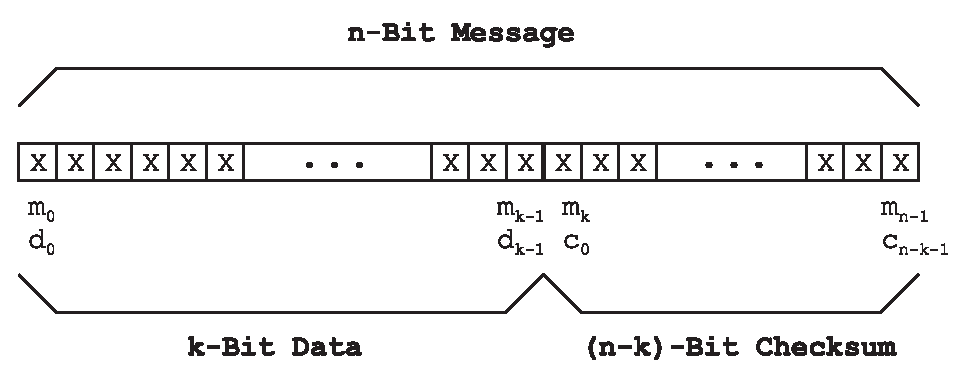
\includegraphics[width=4.6in]{c_edc0/cword01.eps}
\caption{Message Consisting Of The Concatenation Of $k$ Data Bits And $n-k$
         Check Bits, With Bit Notational Conventions}
\label{fig:cedc0:scon0:sccb0:01}
\end{figure}

We have referred to \emph{check bits} without describing the ways in which they
might be calculated.  We use the term \index{checksum}\emph{checksum} to refer
to the contiguous group of $n-k$ check bits; whether or not the bits are calculated
through summation.  In general, we impose only the requirement that the $n-k$-bit 
checksum is a deterministic function of the $k$ data bits.

We often refer to a message or a portion of a message as a 
\index{vector}\emph{vector}.  This nomenclature is appropriate because it is
convenient to treat a message as a row vector of bits.  
An 80-bit message might
be viewed as a $1 \times 80$ matrix (i.e. a row vector) with each matrix element
$\in \mathbb{B}$.  We use \emph{message} and \emph{vector} somewhat interchangeably.

We define the \index{weight}\emph{weight} of a message or vector as the number of 
1's in the message or vector.  We denote the weight of a vector or message $v$ as
$wt(v)$.


%%%%%%%%%%%%%%%%%%%%%%%%%%%%%%%%%%%%%%%%%%%%%%%%%%%%%%%%%%%%%%%%%%%%%%%%%%%%%%%%
%%%%%%%%%%%%%%%%%%%%%%%%%%%%%%%%%%%%%%%%%%%%%%%%%%%%%%%%%%%%%%%%%%%%%%%%%%%%%%%%
%%%%%%%%%%%%%%%%%%%%%%%%%%%%%%%%%%%%%%%%%%%%%%%%%%%%%%%%%%%%%%%%%%%%%%%%%%%%%%%%
\subsection[Codewords, Codes, And \protect\mbox{\protect$(n,k)$} Block Codes]
           {Codewords, Codes And \protect\mbox{\protect\boldmath$(n,k)$} Block Codes}
%Subection tag: cco0
\label{cedc0:scon0:scco0}

A \index{codeword}\emph{codeword} (as we define it here) is a message in which 
the $n-k$ check bits are consistent with the $k$ data bits.
Under this definition, all codewords are messages, but not all possible messages
are codewords.

A common cognitive misconception is that it matters in transmission or
storage whether the $k$ data bits or the $n-k$ check bits are corrupted.
It matters not.  We seek mathematical properties that apply to the messages 
and codewords, not to the $k$ data bits or $n-k$ check bits separately.

In the most general terms, a \index{code}\emph{code} is \emph{any} system
of information representation for transmission, not necessarily requiring 
transmission in fixed-length blocks.  However, in this discussion, by
\emph{code} we mean the set of all bit 
patterns with data and check bits consistent (i.e. all codewords)
which can be transmitted over a communication channel or stored
in computer memory.  For example,
$\{000, 011, 101, 110\}$ is a code.

A code may be specified either by enumeration or by rule.  For example,
we might also specify the code of the previous paragraph as 
$\{ABC: C=A \oplus B\}$.  With larger codes, enumeration is naturally not practical and
also not necessary to study the properties of interest.

An
\index{(n,k) block code@$(n,k)$ block code}\index{n,k block code@$(n,k)$ block code}%
$(n,k)$ \emph{block code} is a code where $n$ bits are transmitted (or stored) at a
time, and characterized by a function which maps from $k$ data bits to $n$ bits which
are transmitted (or stored).

In a general $(n,k)$ block code, the $n$ transmitted
bits are not required to contain or resemble the $k$ data bits; and if the $k$ data bits
are contained they are not required to have a specific order or placement within 
the $n$ transmitted bits.  Because we are interested in adding 
redundancy to ROM and in other applications
where the stored data must be contiguous and unmodified, we confine ourselves
to $(n,k)$ block codes as depicted in Figure
\ref{fig:cedc0:scon0:sccb0:01}, where the $k$ data bits are contiguous, unchanged,
in their original order, and prepended to the $n-k$ check bits.


%%%%%%%%%%%%%%%%%%%%%%%%%%%%%%%%%%%%%%%%%%%%%%%%%%%%%%%%%%%%%%%%%%%%%%%%%%%%%%%%
%%%%%%%%%%%%%%%%%%%%%%%%%%%%%%%%%%%%%%%%%%%%%%%%%%%%%%%%%%%%%%%%%%%%%%%%%%%%%%%%
%%%%%%%%%%%%%%%%%%%%%%%%%%%%%%%%%%%%%%%%%%%%%%%%%%%%%%%%%%%%%%%%%%%%%%%%%%%%%%%%
\subsection{Hamming Distance, Minimum Hamming Distance, And Errors}
%Subection tag: mhd0
\label{cedc0:scon0:smhd0}

We define the \index{Hamming distance}\emph{Hamming distance} between 
two same-length blocks $c$ and $d$, denoted $d(c,d)$, as the number of bit positions
in which the blocks differ.  Note that $d(c,d)$ is necessarily the same as the number
of 1's in $c \oplus d$.  Note also that $d(c,d)$ is the weight of the 
exclusive-OR of $c$ and $d$, i.e. $d(c,d) = wt(c \oplus d)$.  (We discuss the properties 
of the exclusive-OR function later in Section \ref{cedc0:sfft0:dff0}.)

We define the \index{minimum Hamming distance}\emph{minimum Hamming distance}
of a code, denoted $\hat{d}$, as the smallest Hamming distance between any two 
members of the code.  For example, the minimum Hamming distance of
$\{000, 011, 101, 110\}$,
denoted $\hat{d}(\{000, 011, 101, 110\})$,
 is 2, and the minimum Hamming distance of
$\{0001, 0110, 1010, 1101\}$,
denoted $\hat{d}(\{0001, 0110, 1010, 1101\})$,
 is also 2.\footnote{See Exercise 
\ref{exe:cedc0:sexe0:01}.}

We define an \index{error}\emph{error} (or alternatively, a 
\emph{bit corruption} or simply a \emph{corruption}) as the corruption
of a transmitted or stored
bit from 0 to 1 or from 1 to 0.  As mentioned in
Section \ref{cedc0:scon0:sccb0}, we assume that a corruption may occur
with probability $p$ or fail to occur with probability $q=1-p$.

We define a \index{message corruption}\emph{message corruption} or simply 
\emph{corruption} as the corruption of one or more bits within the message
during transmission or storage.
Note that the minimum Hamming distance $\hat{d}$ of a code
guarantees that at least $\hat{d}$ errors are required to transform
one codeword into another, thus guaranteeing that any corruption
of $\hat{d}-1$ or fewer bits is detectable.

If the errors within a message are distributed in a special way, we may be
able to devise codes that are more resistant to these special distributions 
than to an arbitrary distribution of errors.  One such special distribution
is a \index{burst error}\emph{burst error}.  A \emph{burst error of length $b$}
is defined as any number of errors in a span of $b$ bits.  For example, corruption of
00001111 to 00011001 represents a burst error of length 4 (the corruptions are in 
the 4th, 6th, and 7th bits, which span 4 bits inclusive).  A burst error may naturally
span no fewer than 1 bit and no more than $n$ bits.

We are very careful \emph{not} to define a codeword as an
uncorrupted message.  No code except a code consisting of only one codeword
can sustain an unlimited number of bit corruptions while still guaranteeing
that the message corruption will be detectable.\footnote{This observation that
a single-codeword code can sustain an unlimited number of bit corruptions is a
mathematical fallacy and a semantic parlor trick.  An $(n,k)$ block code with only
one code word effectively has a maximum Hamming distance $\hat{d}$ of $n$ plus the number
of framing bits, stop bits, etc. in the message as transmitted.  Sufficient noise
in a communication channel may cause communication hardware to believe the
codeword was transmitted when in fact it was not.  See the remarks regarding
framing weaknesses in Section \ref{cedc0:scon0:sccb0}.}  A codeword may in fact
be a corrupted message where the number of bit corruptions has overwhelmed the 
minimum Hamming distance $\hat{d}$ of the code so as to transform one codeword
into another.

Generally, error-detecting and error-correcting codes
(Section \ref{cedc0:scon0:secv0}) must be selected with some knowledge 
of the error
rates of the 
communication channel or storage medium.  Noisier communication channels 
or poorer storage mediums require codes with
better error-detecting and/or error-correcting properties.  Normally, the design goal
is to achieve a very low probability of undetected corruption or uncorrectable corruption.


%%%%%%%%%%%%%%%%%%%%%%%%%%%%%%%%%%%%%%%%%%%%%%%%%%%%%%%%%%%%%%%%%%%%%%%%%%%%%%%%
%%%%%%%%%%%%%%%%%%%%%%%%%%%%%%%%%%%%%%%%%%%%%%%%%%%%%%%%%%%%%%%%%%%%%%%%%%%%%%%%
%%%%%%%%%%%%%%%%%%%%%%%%%%%%%%%%%%%%%%%%%%%%%%%%%%%%%%%%%%%%%%%%%%%%%%%%%%%%%%%%
\subsection{Error-Detecting Versus Error-Correcting Codes}
%Subection tag: ecv0
\label{cedc0:scon0:secv0}

An \index{error-detecting code}\emph{error-detecting code} is a code which is
designed so that message errors
(a message which is not a codeword) will be detected but not corrected.  
Error-detecting codes are attractive
when there is the opportunity to request that the transmitter retransmit the 
corrupted data, or when obtaining a correct copy of the data is not important but
detecting (and perhaps discarding) corrupted data is important.

An \index{error-correcting code}\emph{error-correcting code} is a code designed 
so that message errors can be both detected and corrected.  Error-correcting 
codes are attractive when 
there is no opportunity for retransmission of the corrupted data, but possessing
a correct copy of the data is important.  Example attractive 
applications of error-correcting codes are compact disc audio data (where the
CD should play even with scratches, and there is no opportunity to obtain
retransmission of the data) and data transmitted from space exploration satellites
(where the signal-to-noise ratio is low, and there is not opportunity for retransmission
or perhaps not even two-way communication).

In this section we show the required relationship between minimum Hamming
distance $\hat{d}$ and the error-detecting and error-correcting capabilities
of a code.

We define the \index{error-detecting capability of a code}\index{code!error-detecting capability}%
\emph{error-detecting capability} $d_{ED}$ of a code as the largest number of bit errors 
in a message which will \emph{always} be detectable.  It follows
immediately and intuitively that 

\begin{equation}
\label{eq:cedc0:scon0:secv0:01}
d_{ED} = \hat{d} - 1 .
\end{equation}

\noindent{}If the minimum 
Hamming distance of a code is $\hat{d}$, then there exists at least
one pair of codewords
$c_1, c_2$ such that $d(c_1, c_2) = \hat{d}$.  Thus it is possible to corrupt
$c_1$ into $c_2$ with $\hat{d}$ corrupted bits and therefore
$d_{ED} < \hat{d}$.  On the other hand, the minimum Hamming distance 
$\hat{d}$ guarantees that it is \emph{not} possible to corrupt from one codeword to another
with only $\hat{d}-1$ bit corruptions.  Therefore
(\ref{eq:cedc0:scon0:secv0:01}) is true.

We define the \index{error correcting capability of a code}\index{code!error correcting capability}%
\emph{error correcting capability} $d_{EC}$ of a code  as the largest number of bit errors 
in a message which will \emph{always} be correctable.  By \emph{correctable} we mean
that we can recover the original $n$-bit codeword into which errors were introduced.

To illustrate the relationship between Hamming distance and the error correcting
capability of a code, consider the code $\{000, 111\}$ depicted in
Figure \ref{fig:cedc0:scon0:secv0:01}.  In the figure, each edge in the cube depicts
a single bit error which may occur in a message.  Each vertex in the cube 
represents a message.

\begin{figure}
\centering
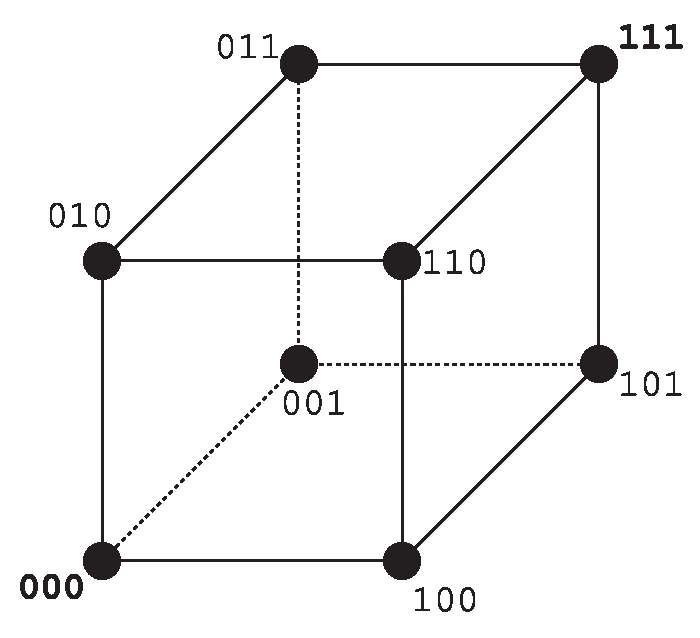
\includegraphics[height=2.5in]{c_edc0/cube01.eps}
\caption{Three-Dimensional Cube Illustrating Error Correction With Code $\{000, 111\}$}
\label{fig:cedc0:scon0:secv0:01}
\end{figure}

Note that the minimum Hamming $\hat{d}$ distance of the code $\{000, 111\}$ is 3:  in
Figure \ref{fig:cedc0:scon0:secv0:01} one must travel along three edges
(corresponding to three bit errors) in order to travel from 000 to 111 or back.

If we claim that a code has an error correcting capability of $d_{EC}$, 
then any corruption of a codeword by $d_{EC}$ errors must be correctable.
To be \emph{correctable} means that if we guess based on the corrupted
codeword what the original codeword is, we must always be able to guess
correctly.  This notion implies that the original codeword must be the 
closest codeword (as measured by number of bit corruptions) to the corrupted codeword.

This notion of \emph{closest} codeword leads to the notion of a \emph{packing sphere}.
A \emph{packing sphere of radius $\rho$} is the set of all messages
at a distance of $\rho$ or less from a given codeword.  In order for 
a code to have an error correcting capability of $d_{EC}=\rho$, 
the packing spheres or radius $\rho$ about all codewords must be disjoint.
This ensures that any message at a distance $d_{EC}$ or less from a codeword
does, in fact, have a \emph{nearest} codeword.

Figure \ref{fig:cedc0:scon0:secv0:02} is
Figure \ref{fig:cedc0:scon0:secv0:01} redrawn to show the packing spheres of
radius $\rho=1$ about the two codewords 000 and 111.  The code
$\{000,111\}$ depicted in Figures \ref{fig:cedc0:scon0:secv0:01} and
\ref{fig:cedc0:scon0:secv0:02} has an error correcting capability of 
$d_{EC}=1$.  For error correction, any message in the packing sphere
about 000 must be mapped back to 000, and any message in the packing sphere
about 111 must be transformed back to 111.

\begin{figure}
\centering
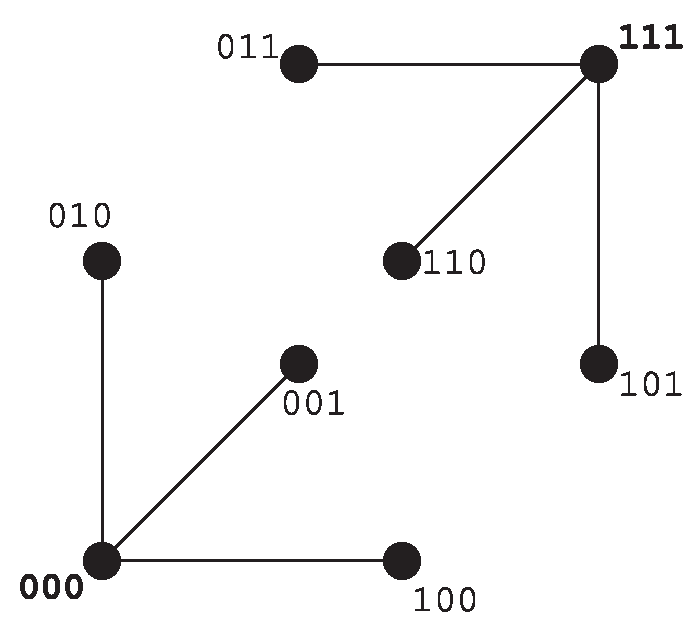
\includegraphics[height=2.5in]{c_edc0/cube02.eps}
\caption{Packing Spheres Of Radius $\rho{}=1$ About Codewords 000 And 111}
\label{fig:cedc0:scon0:secv0:02}
\end{figure}

The requirement for disjointness of packing spheres immediately leads to
the constraint

\begin{equation}
\label{eq:cedc0:scon0:secv0:02}
\hat{d} > 2 \rho 
\end{equation}

\noindent{}or equivalently when considering only integers that

\begin{equation}
\label{eq:cedc0:scon0:secv0:03}
\hat{d} \geq 2 \rho + 1 . 
\end{equation}

\noindent{}Since the radius $\rho$ of the packing sphere is 
equivalent to the error correcting capability $d_{EC}$ of
a code, we may equivalently write 
(\ref{eq:cedc0:scon0:secv0:02}) and (\ref{eq:cedc0:scon0:secv0:03})
as $\hat{d} > 2 d_{EC}$ and $\hat{d} \geq 2 d_{EC} + 1$, respectively.

(\ref{eq:cedc0:scon0:secv0:02}) and (\ref{eq:cedc0:scon0:secv0:03})
treat minimum Hamming distance $\hat{d}$ as a function of 
the packing sphere radius $\rho$.  With a known minimum Hamming distance 
$\hat{d}$, one may also calculate the largest disjoint
packing spheres that can be constructed:

\begin{equation}
\label{eq:cedc0:scon0:secv0:04}
d_{EC} = \rho = \left\lfloor {\frac{\hat{d}-1}{2}} \right\rfloor .
\end{equation}

This section has demonstrated the relationship between the minimum Hamming
distance $\hat{d}$ of a code and the error detection capability of the code
(Equation \ref{eq:cedc0:scon0:secv0:01}), as well as the relationship between the
minimum Hamming
distance $\hat{d}$ and the error correction capabilility 
(Equations \ref{eq:cedc0:scon0:secv0:02} through 
\ref{eq:cedc0:scon0:secv0:04}).

Note that the relationships derived do apply to the example presented in 
Figures \ref{fig:cedc0:scon0:secv0:01} and \ref{fig:cedc0:scon0:secv0:02}.
The code shown in the figures has a minimum Hamming distance $\hat{d}=3$.
(\ref{eq:cedc0:scon0:secv0:01}) predicts that this code should have
an error detection capability of $d_{ED}=2$, which is the case.  
(\ref{eq:cedc0:scon0:secv0:04}) predicts that this code should have an error correction
capability $d_{EC}=1$, which is also the case and can be verified by
examining Figure \ref{fig:cedc0:scon0:secv0:02}.

In the code presented in Figures \ref{fig:cedc0:scon0:secv0:01} and 
\ref{fig:cedc0:scon0:secv0:02}, the union of all packing spheres of radius 
$\rho=1$ contains all messages (i.e. there are no messages which are not part of
a packing sphere).  Such a code is called a \emph{perfect code}.  Most codes
are not perfect codes, and this will be discussed later.


%%%%%%%%%%%%%%%%%%%%%%%%%%%%%%%%%%%%%%%%%%%%%%%%%%%%%%%%%%%%%%%%%%%%%%%%%%%%%%%%
%%%%%%%%%%%%%%%%%%%%%%%%%%%%%%%%%%%%%%%%%%%%%%%%%%%%%%%%%%%%%%%%%%%%%%%%%%%%%%%%
%%%%%%%%%%%%%%%%%%%%%%%%%%%%%%%%%%%%%%%%%%%%%%%%%%%%%%%%%%%%%%%%%%%%%%%%%%%%%%%%
\section[Finite Field Theory Applied To \protect\mbox{\protect$\mathbb{B}$}]
        {Finite Field Theory Applied To \protect\mbox{\protect\boldmath$\mathbb{B}$}}
%Section tag: fft0
\label{cedc0:sfft0}

This 
section  deals with \index{finite field}finite field 
theory as applied to the binary alphabet,
$\mathbb{B} = \{ 0, 1 \}$.
This section is one of two sections in this chapter which deal with 
\index{finite field}finite field theory 
(the other section is Section \ref{cedc0:sfft1},
which deals with finite field theory as applied to polynomials).  


%%%%%%%%%%%%%%%%%%%%%%%%%%%%%%%%%%%%%%%%%%%%%%%%%%%%%%%%%%%%%%%%%%%%%%%%%%%%%%%%
%%%%%%%%%%%%%%%%%%%%%%%%%%%%%%%%%%%%%%%%%%%%%%%%%%%%%%%%%%%%%%%%%%%%%%%%%%%%%%%%
%%%%%%%%%%%%%%%%%%%%%%%%%%%%%%%%%%%%%%%%%%%%%%%%%%%%%%%%%%%%%%%%%%%%%%%%%%%%%%%%
\subsection{\emph{Why} Field Theory?}
%Subection tag: wft0
\label{cedc0:sfft0:wft0}

The most important question to answer immediately (for engineers, anyway)
is \emph{why} field theory is necessary at all.  The answer is that
there are two general approaches that can be used to approach coding
theory:

\begin{enumerate}
\item \emph{Combinational:} 
      approaching the problem by considering combinations and
      permutations (see Section \ref{cedc0:scob0}, for example).  This approach
      can give some insight and produce useful bounds, but in general it is hard
      to approach the problem of generating codes with an arbitrarily large minimum
      Hamming distance $\hat{d}$ using a purely combinational approach.
\item \emph{Field Theory:} approaching the problem by attempting to add algebraic
      structure to codes.  This approach leads to classes of solutions that
      are unavailable using purely combinational approaches.  To add
      \emph{algebraic structure} means to define operations so as to add useful
      algebraic properties that facilitate higher-level inferences
      and abstractions.  For example,
      algebraic structure is ultimately what allows us to define the rank
      of a matrix with elements $\in \mathbb{B}$ in the same way we do with
      matrices with elements $\in \vworkrealset$.
\end{enumerate}

Note that combinational and field theory approaches are complementary:  each
approach gives some unique insight and solutions that the other approach cannot
provide.

Field theory is necessary in order to derive a framework in which to 
systematically generate codes with a large minimum Hamming distance $\hat{d}$.


%%%%%%%%%%%%%%%%%%%%%%%%%%%%%%%%%%%%%%%%%%%%%%%%%%%%%%%%%%%%%%%%%%%%%%%%%%%%%%%%
%%%%%%%%%%%%%%%%%%%%%%%%%%%%%%%%%%%%%%%%%%%%%%%%%%%%%%%%%%%%%%%%%%%%%%%%%%%%%%%%
%%%%%%%%%%%%%%%%%%%%%%%%%%%%%%%%%%%%%%%%%%%%%%%%%%%%%%%%%%%%%%%%%%%%%%%%%%%%%%%%
\subsection{Definition Of A Finite Field}
%Subection tag: dff0
\label{cedc0:sfft0:dff0}

We first define what a \index{finite field} \emph{finite field} is in general, and 
then we show how this definition is applied to $\mathbb{B} = \{ 0, 1 \}$.

\begin{vworkdefinitionstatementpar}{Finite Field}
A \emph{finite field} \cite{bibref:w:weissteinmathworld}
is a finite set of elements (the cardinality of this
set is called the \index{field order}\emph{field order}) which 
satisfies the field axioms
listed in Table \ref{tbl:cedc0:sfft0:dff0:01} for both addition and
multiplication.

\begin{table}
\caption{Field Axioms For A Finite Field (From \cite{bibref:w:weissteinmathworld})}
\label{tbl:cedc0:sfft0:dff0:01}
\begin{center}
\begin{tabular}{|l|c|c|}
\hline
Name           &  Addition             & Multiplication       \\
\hline
\hline
Commutativity  & $a+b = b+a$           & $ab = ba$             \\
\hline
Associativity  & $(a+b)+c=a+(b+c)$     & $(ab)c=a(bc)$         \\
\hline
Distributivity & $a(b+c)=ab+ac$        & $(a+b)c=ac+bc$        \\
\hline
Identity       & $a+0=a=0+a$           & $a \cdot 1=a=1 \cdot a$ \\
\hline
Inverses       & $a+(-a)=0=(-a)+a$     & $aa^{-1}=1=a^{-1}a$ if $a \neq 0$ \\
\hline
\end{tabular}
\end{center}
\end{table}

Such a field is also called a \index{Galois field}\emph{Galois field}.
In this chapter, we are concerned with the Galois field containing
only two elements ($\mathbb{B}=\{ 0,1 \}$), and this field is denoted $GF(2)$.
\end{vworkdefinitionstatementpar}
\vworkdefinitionfooter{}

The study of fields is a topic from \index{abstract algebra}\emph{abstract algebra},
a branch of mathematics.  This chapter provides only the
minimum amount of information about finite field theory to explain
the presented application, and so there are many mathematical results 
not discussed.

The definition of a finite field (Definition \ref{tbl:cedc0:sfft0:dff0:01}) 
does not specify how addition and multiplication are defined---it only
specifies what properties must be met by whatever choice is made.
We now present the only possible choices for addition, multiplication,
formation of the additive inverse, and formation of the multiplicative inverse
for the elements of $\mathbb{B}=\{ 0,1 \}$.

Addition (Table \ref{tbl:cedc0:sfft0:dff0:02}) is performed modulo 2, and is 
identical to the exclusive-OR 
function.  In computer software, this function is normally implemented using
the XOR machine instruction, which operates on many bits in parallel.  Although
we would be justified in using `$+$' to denote this operation, instead we
use `$\oplus$' because it corresponds more closely to the machine instruction
actually used to implement this binary operation.

\begin{table}
\caption{Truth Table Of Addition Over $\mathbb{B}=\{ 0,1 \}$ (Denoted $\oplus$)}
\label{tbl:cedc0:sfft0:dff0:02}
\begin{center}
\begin{tabular}{|c|c|c|}
\hline
$a$           &  $b$                  & $c = a \oplus b$     \\
\hline
\hline
0             & 0                     & 0                     \\
\hline
0             & 1                     & 1                     \\
\hline
1             & 0                     & 1                     \\
\hline
1             & 1                     & 0                     \\
\hline
\end{tabular}
\end{center}
\end{table}

Subtraction is equivalent to adding the additive inverse.  
Table \ref{tbl:cedc0:sfft0:dff0:03} provides the
additive inverses of the field elements 0 and 1.  Table
\ref{tbl:cedc0:sfft0:dff0:04} is the truth table for subtraction.

\begin{table}
\caption{Truth Table Of Additive Inverse Over $\mathbb{B}=\{ 0,1 \}$}
\label{tbl:cedc0:sfft0:dff0:03}
\begin{center}
\begin{tabular}{|c|c|}
\hline
$a$           &  $-a$                 \\
\hline
\hline
0             & 0                     \\
\hline
1             & 1                     \\
\hline
\end{tabular}
\end{center}
\end{table}

\begin{table}
\caption{Truth Table Of Subtraction Over $\mathbb{B}=\{ 0,1 \}$ (Denoted $-$)}
\label{tbl:cedc0:sfft0:dff0:04}
\begin{center}
\begin{tabular}{|c|c|c|}
\hline
$a$           &  $b$                  & $c = a - b = a + (-b)$     \\
\hline
\hline
0             & 0                     & 0                     \\
\hline
0             & 1                     & 1                     \\
\hline
1             & 0                     & 1                     \\
\hline
1             & 1                     & 0                     \\
\hline
\end{tabular}
\end{center}
\end{table}


Table \ref{tbl:cedc0:sfft0:dff0:05} supplies the definition of the 
multiplication operation in $GF(2)$.

\begin{table}
\caption{Truth Table Of Multiplication Over $\mathbb{B}=\{ 0,1 \}$}
\label{tbl:cedc0:sfft0:dff0:05}
\begin{center}
\begin{tabular}{|c|c|c|}
\hline
$a$           &  $b$                  & $c = a b$             \\
\hline
\hline
0             & 0                     & 0                     \\
\hline
0             & 1                     & 0                     \\
\hline
1             & 0                     & 0                     \\
\hline
1             & 1                     & 1                     \\
\hline
\end{tabular}
\end{center}
\end{table}

Table \ref{tbl:cedc0:sfft0:dff0:06} supplies the definition of the 
multiplicative inverse over $GF(2)$.  Note that division is assumed
to be the same as multiplication by the multiplicative inverse.
As required by the definition of a field, division by 0 is not
defined.

\begin{table}
\caption{Truth Table Of Multiplicative Inverse Over $\mathbb{B}=\{ 0,1 \}$}
\label{tbl:cedc0:sfft0:dff0:06}
\begin{center}
\begin{tabular}{|c|c|}
\hline
$a$           &  $a^{-1}$             \\
\hline
\hline
0             & Undefined             \\
\hline
1             & 1                     \\
\hline
\end{tabular}
\end{center}
\end{table}

There are unique properites of calculations within
$GF(2)$.  We summarize these unique properties here.

\begin{enumerate}
\item \label{prop:enum:cedc0:sfft0:dff0:01:01}
      Addition and subtraction
      are identical.  This means that we can always replace `$-$' with `$\oplus$',
      and it also means we can break the usual rules of algebra and simply
      ``drag'' terms joined by `$\oplus$' from one side of an equality to the other.
      Specifically, 

      \begin{equation}
      \label{eq:cedc0:sfft0:dff0:01}
      (a = b \oplus c) \vworkequiv (a \oplus b = c) \vworkequiv (a \oplus b \oplus c = 0) .
      \end{equation}

\item \label{prop:enum:cedc0:sfft0:dff0:01:02}
      Adding any value to itself
      yields $0$.  This comes directly because $0 \oplus 0 = 1 \oplus 1=0$.
      This allows the removal of pairs of identical values joined by 
      $\oplus$, i.e. 

      \begin{equation}
      \label{eq:cedc0:sfft0:dff0:02}
      1 \oplus 1 \oplus a \oplus b \oplus a \oplus b \oplus a \oplus b \oplus a = b.
      \end{equation}
\end{enumerate}


%%%%%%%%%%%%%%%%%%%%%%%%%%%%%%%%%%%%%%%%%%%%%%%%%%%%%%%%%%%%%%%%%%%%%%%%%%%%%%%%
%%%%%%%%%%%%%%%%%%%%%%%%%%%%%%%%%%%%%%%%%%%%%%%%%%%%%%%%%%%%%%%%%%%%%%%%%%%%%%%%
%%%%%%%%%%%%%%%%%%%%%%%%%%%%%%%%%%%%%%%%%%%%%%%%%%%%%%%%%%%%%%%%%%%%%%%%%%%%%%%%
\subsection[Properties Of Matrices Consisting Of Elements \mbox{\protect$\in \mathbb{B}$}]
           {Properties Of Matrices Consisting Of Elements \mbox{\protect\boldmath$\in \mathbb{B}$}}
%Subection tag: rmc0
\label{cedc0:sfft0:rmc0}

In high school and college, most engineers studied linear algebra using 
matrices with elements $\in \vworkrealset$.  The set of real numbers combined
with the traditional addition and multiplication operators is
an \emph{infinite} field, whereas the set $\mathbb{B} = \{ 0, 1 \}$ combined
with the addition and multiplication operators as defined in
Section \ref{cedc0:sfft0:dff0} is a \emph{finite} field, namely 
$GF(2)$.  It may not be clear to a practicing engineer whether the traditional notions
from linear algebra apply to the finite field $GF(2)$ as 
defined here.

It ends up that all of the traditional notions from linear algebra
\emph{do} apply to finite fields and to $GF(2)$.  Most undergraduate linear
algebra texts, however, do not develop this.  By 
\emph{traditional notions} we mean:

\begin{itemize}
\item The notion of the rank of a matrix.
\item The notion of the determinant of a matrix (denoted $|A|$ or $det(A)$).
\item The equivalence of all of the following statements:
      \begin{itemize}
      \item $|A_{n \times n}| = 0$.
      \item $A$ is not of full rank.
      \item Any linear combination of the rows or columns of $A$ can span
            only a subspace of $\mathbb{B}^n$.
      \end{itemize}
\end{itemize}

The notion of subspace, however, has a subtly different flavor with a finite
field because such a subspace has a finite and countable number of elements.
With that in mind, we present the following lemma.

\begin{vworklemmastatement}
\label{lem:cedc0:sfft0:rmc0:01}
Linear combinations of the
rows or columns from an
$m \times n$ matrix $A$ with elements from $\mathbb{B}$ and with
rank $r$ can span exactly $2^r$ vectors.
\end{vworklemmastatement}
\begin{vworklemmaproof}
For simplicity assume a square matrix $A_{n \times n}$ with rank
$r \leq n$ (the result applies also to non-square matrices and to
the columns as well as the rows).
Denote the rows of $A$ as $r_0 \ldots r_{n-1}$.
Sort the rows of the matrix so that $r_0 \ldots{} r_{r-1}$ are linearly
independent and rows $r_{r} \ldots{} r_{n-1}$ are each linear combinations
of $r_0 \ldots{} r_{r-1}$.

Consider the $2^n$ linear combinations of the 
$n$ rows, with each linear combination of the 
form $\alpha_0 r_0 + \alpha_1 r_1 + \ldots{} + \alpha_{n-1} r_{n-1}$,
where $\alpha_i \in \mathbb{B}$.  For those linear combinations
where there are nonzero $\alpha_{r} \ldots{} \alpha_{n-1}$, since 
each $r_{r} \ldots{} r_{n-1}$ is a linear combination of 
$r_0 \ldots{} r_{r-1}$, a substitution can be made to express the 
linear combination as a sum of $r_0 \ldots{} r_{r-1}$ only, and then 
superfluous terms can be removed in pairs
(Property \ref{prop:enum:cedc0:sfft0:dff0:01:02}, p. \pageref{prop:enum:cedc0:sfft0:dff0:01:02})
to give a linear combination of $r_0 \ldots{} r_{r-1}$ only.
Thus, every $\alpha_0 r_0 + \alpha_1 r_1 + \ldots{} + \alpha_{n-1} r_{n-1}$
can be simplified to $\alpha_0 r_0 + \alpha_1 r_1 + \ldots{} + \alpha_{r-1} r_{r-1}$.
Since no row $r_0 \ldots r_{r-1}$ is a linear combination of other rows
$r_0 \ldots r_{r-1}$, each of the $2^r$ linear combinations 
is unique and thus all linear combinations of the rows
sum to one of $2^r$ distinct $1 \times n$ vector values.
\end{vworklemmaproof}
\vworklemmafooter{}

The ability to directly apply concepts from linear algebra to matrices
with elements $\in \mathbb{B}$ is in fact the reason for employing finite field
theory.  We illustrate the applicability of standard linear algebra concepts to these
types of matrices with the following example.

\begin{vworkexamplestatement}
\label{ex:cedc0:sfft0:rmc0:01}
Consider the two matrices $A$ and $B$ with elements $\in \mathbb{B}$:

\begin{equation}
\label{eq:cedc0:sfft0:rmc0:01}
A = \left[\begin{array}{ccc}1&1&0\\0&1&1\\1&0&1\end{array}\right], \;\;
B = \left[\begin{array}{ccc}1&1&0\\0&1&1\\0&0&1\end{array}\right].
\end{equation}

Determine the rank of $A$ and $B$ and the set of $1 \times 3$ vectors
which is spanned by linear combination of their rows.
\end{vworkexamplestatement}
\begin{vworkexampleparsection}{Solution}
Recall that for a $3 \times 3$ matrix
$\left[\begin{array}{ccc}a&b&c\\d&e&f\\g&h&i\end{array}\right]$,
the determinant is given by
$a(ei-hf) - b(di-gf) + c(dh - ge)$.  However, with
elements from $GF(2)$, addition and subtraction are the same 
operation (Property \ref{prop:enum:cedc0:sfft0:dff0:01:01}, p. \pageref{prop:enum:cedc0:sfft0:dff0:01:01}),
so we can replace `-' and '+' both with `$\oplus$' to give the
simpler expression 
$a(ei \oplus hf) \oplus b(di \oplus gf) \oplus c(dh \oplus ge)$.  The
determinants of $A$ and $B$ are thus

\begin{eqnarray}
\nonumber
|A| & = & 1 (1 \cdot 1 \oplus 0 \cdot 1) \oplus
          1 (0 \cdot 1 \oplus 1 \cdot 1) \oplus
          0 (0 \cdot 0 \oplus 1 \cdot 1)          \\
\label{eq:cedc0:sfft0:rmc0:02}
    & = & 1 (1 \oplus 0) \oplus 1 (0 \oplus 1) \oplus 0 (0 \oplus 1) \\
\nonumber
    & = & 1 \oplus 1 \oplus 0 = 0
\end{eqnarray}

\noindent{}and

\begin{eqnarray}
\nonumber
|B| & = & 1 (1 \cdot 1 \oplus 0 \cdot 1) \oplus
          1 (0 \cdot 1 \oplus 0 \cdot 1) \oplus
          0 (0 \cdot 1 \oplus 0 \cdot 1)          \\
\label{eq:cedc0:sfft0:rmc0:03}
    & = & 1 (1 \oplus 0) \oplus 1 (0 \oplus 0) \oplus 0 (0 \oplus 0) \\
\nonumber
    & = & 1 \oplus 0 \oplus 0 = 1  .
\end{eqnarray}

From the determinants, it follows that $B$ is of full rank ($rank(B)=3$) but $A$ is not.  
In fact,
it can be seen on inspection of $A$ that the third row is the sum of the first
two rows ($rank(A) = 2$).

To enumerate the space spanned by the rows of $A$ and $B$, one can form the sum
$\alpha_0 r_0 \oplus \alpha_1 r_1 \oplus \alpha_2 r_2$ and vary the parameters
$\alpha_0, \alpha_1, \alpha_2 \in \mathbb{B}$.  
Table \ref{tbl:cedc0:sfft0:rmc0:01} supplies this range for
$A$ and Table \ref{tbl:cedc0:sfft0:rmc0:02} supplies this range
for $B$.

\begin{table}
\caption{Range Of $\alpha_0 r_0 \oplus \alpha_1 r_1 \oplus \alpha_2 r_2$ For $A$ Of Example \ref{ex:cedc0:sfft0:rmc0:01}}
\label{tbl:cedc0:sfft0:rmc0:01}
\begin{center}
\begin{tabular}{|c|c|c|l|}
\hline
$\alpha_0$           &  $\alpha_1$                  & $\alpha_2$ &   $\alpha_0 [1 \; 1 \; 0] \oplus \alpha_1 [0 \; 1 \; 1] \oplus \alpha_2 [1 \; 0 \; 1]$   \\
\hline
\hline
0  & 0  & 0  & $[0\;0\;0]$ \\
\hline
0  & 0  & 1  & $[1\;0\;1]$ \\
\hline
0  & 1  & 0  & $[0\;1\;1]$ \\
\hline
0  & 1  & 1  & $[0\;1\;1] \oplus [1\;0\;1]$ \\
   &    &    & $[0 \oplus 1 \;\; 1 \oplus 0\;\; 1 \oplus 1]$ \\
   &    &    & $[1\;1\;0]$ \\
\hline
1  & 0  & 0  & $[1\;1\;0]$ \\
\hline
1  & 0  & 1  & $[1\;1\;0] \oplus [1\;0\;1]$ \\
   &    &    & $[1 \oplus 1 \;\; 1 \oplus 0\;\; 0 \oplus 1]$ \\
   &    &    & $[0\;1\;1]$ \\
\hline
1  & 1  & 0  & $[1\;1\;0] \oplus [0\;1\;1]$ \\
   &    &    & $[1 \oplus 0 \;\; 1 \oplus 1\;\; 0 \oplus 1]$ \\
   &    &    & $[1\;0\;1]$ \\
\hline
1  & 1  & 1  & $[1\;1\;0] \oplus [0\;1\;1] \oplus [1\;0\;1]$ \\
   &    &    & $[1 \oplus 0 \oplus 1 \;\; 1 \oplus 1 \oplus 0\;\; 0 \oplus 1 \oplus 1]$ \\
   &    &    & $[0\;0\;0]$ \\
\hline
\end{tabular}
\end{center}
\end{table}

\begin{table}
\caption{Range Of $\alpha_0 r_0 \oplus \alpha_1 r_1 \oplus \alpha_2 r_2$ For $B$ Of Example \ref{ex:cedc0:sfft0:rmc0:01}}
\label{tbl:cedc0:sfft0:rmc0:02}
\begin{center}
\begin{tabular}{|c|c|c|l|}
\hline
$\alpha_0$           &  $\alpha_1$                  & $\alpha_2$ &   $\alpha_0 [1 \; 1 \; 0] \oplus \alpha_1 [0 \; 1 \; 1] \oplus \alpha_2 [0 \; 0 \; 1]$   \\
\hline
\hline
0  & 0  & 0  & $[0\;0\;0]$ \\
\hline
0  & 0  & 1  & $[0\;0\;1]$ \\
\hline
0  & 1  & 0  & $[0\;1\;1]$ \\
\hline
0  & 1  & 1  & $[0\;1\;1] \oplus [0\;0\;1]$ \\
   &    &    & $[0 \oplus 0 \;\; 1 \oplus 0\;\; 1 \oplus 1]$ \\
   &    &    & $[0\;1\;0]$ \\
\hline
1  & 0  & 0  & $[1\;1\;0]$ \\
\hline
1  & 0  & 1  & $[1\;1\;0] \oplus [0\;0\;1]$ \\
   &    &    & $[1 \oplus 0 \;\; 1 \oplus 0\;\; 0 \oplus 1]$ \\
   &    &    & $[1\;1\;1]$ \\
\hline
1  & 1  & 0  & $[1\;1\;0] \oplus [0\;1\;1]$ \\
   &    &    & $[1 \oplus 0 \;\; 1 \oplus 1\;\; 0 \oplus 1]$ \\
   &    &    & $[1\;0\;1]$ \\
\hline
1  & 1  & 1  & $[1\;1\;0] \oplus [0\;1\;1] \oplus [0\;0\;1]$ \\
   &    &    & $[1 \oplus 0 \oplus 0 \;\; 1 \oplus 1 \oplus 0\;\; 0 \oplus 1 \oplus 1]$ \\
   &    &    & $[1\;0\;0]$ \\
\hline
\end{tabular}
\end{center}
\end{table}

Note from the tables that the rows of $A$ span 4 vectors 
(000, 011, 101, and 110), which is consistent 
by Lemma \ref{lem:cedc0:sfft0:rmc0:01} with a matrix of rank 2.
Note also that the rows of $B$ span the full space of
$2^3$ vectors (000, 001, 010, 011, 100, 101, 110, and 111), which
is consistent with a full-rank matrix.
\end{vworkexampleparsection}
\vworkexamplefooter{}


%%%%%%%%%%%%%%%%%%%%%%%%%%%%%%%%%%%%%%%%%%%%%%%%%%%%%%%%%%%%%%%%%%%%%%%%%%%%%%%%
%%%%%%%%%%%%%%%%%%%%%%%%%%%%%%%%%%%%%%%%%%%%%%%%%%%%%%%%%%%%%%%%%%%%%%%%%%%%%%%%
%%%%%%%%%%%%%%%%%%%%%%%%%%%%%%%%%%%%%%%%%%%%%%%%%%%%%%%%%%%%%%%%%%%%%%%%%%%%%%%%
\section[Combinatoric Observations]
        {Combinatoric Observations About \protect\mbox{\protect\boldmath$(n,k)$} Block Codes}
%Section tag: cob0
\label{cedc0:scob0}

A surprising number of observations about $(n,k)$ block codes can be made by
simply considering combinatoric aspects of the codes.  In Section 
\ref{cedc0:scon0:sccb0} and Figure \ref{fig:cedc0:scon0:sccb0:01} 
(p. \pageref{fig:cedc0:scon0:sccb0:01}), no assumptions about the function which
maps from the $k$ data bits to the $n-k$ checksum bits (other than determinism)
were made.  Even with only the assumption of determinism, a large number of properties
can be derived or deduced, and we do this here.  In the following 
subsections, it may be necessary to make slightly stronger assumptions in order
to derive properties.


%%%%%%%%%%%%%%%%%%%%%%%%%%%%%%%%%%%%%%%%%%%%%%%%%%%%%%%%%%%%%%%%%%%%%%%%%%%%%%%%
%%%%%%%%%%%%%%%%%%%%%%%%%%%%%%%%%%%%%%%%%%%%%%%%%%%%%%%%%%%%%%%%%%%%%%%%%%%%%%%%
%%%%%%%%%%%%%%%%%%%%%%%%%%%%%%%%%%%%%%%%%%%%%%%%%%%%%%%%%%%%%%%%%%%%%%%%%%%%%%%%
\subsection[Packing Spheres Of Radius \protect\mbox{\protect$\rho$}]
        {Surface Area And Volume Of Packing Spheres Of Radius \protect\mbox{\protect\boldmath$\rho$}}
%Subsection tag: psr0
\label{cedc0:scob0:psr0}

As discussed in Section \ref{cedc0:scon0:sccb0}, we are interested in constructing
messages consisting of $n$ symbols from the binary alphabet

\begin{equation}
\label{eq:cedc0:scob0:psr0:01}
\mathbb{B} = \{ 0, 1 \} ,
\end{equation}

\noindent{}with $k$ symbols being arbitrarily chosen (data), and the remaining
$n-k$ symbols being check bits.

As mentioned in Section \ref{cedc0:scon0:secv0}, the minimum Hamming distance 
$\hat{d}$
of a
code is related to its error detection capability (Eq. \ref{eq:cedc0:scon0:secv0:01})
and to its error correction capability (Eq. \ref{eq:cedc0:scon0:secv0:04}).
It is most natural to think of the minimum Hamming distance $\hat{d}$ of a code
in terms of disjoint packing spheres or radius $\rho$, where $\hat{d} = 2 \rho + 1$,
rather than considering Hamming distance directly.  In this section, we
derive the surface area\footnote{To use \emph{surface area} in this way is perhaps
a mild abuse of nomenclature.} and volume of packing spheres.

We define the surface area of a packing sphere of radius $\rho$ to be the 
number of messages which are exactly at Hamming distance $\rho$ from a message
being considered.  To say that a message $c_2$ is exactly at distance
$\rho$ from $c_1$ is equivalent to saying that the error vector has weight $\rho$.

Thus, for an $(n,k)$ block code, the number of messages that are precisely
at a distance $\rho$ from another message is given by

\begin{equation}
\label{eq:cedc0:scob0:psr0:02}
S(n, \rho ) = \left({\begin{array}{cc}n\\\rho\end{array}}\right) .
\end{equation}

\noindent{}This formula comes directly from considering the
number of $n$-bit error vectors of weight $\rho$ that can be constructed.

We define the volume of a packing sphere of radius $\rho$ to be the
number of messages which are at a distance $\rho$ or less from a 
message being considered.  This volume can be obtained by 
simply summing the number of messages at distances
$0 \leq d \leq \rho$ from the message being considered:

\begin{eqnarray}
\label{eq:cedc0:scob0:psr0:03}
V(n, \rho ) & = & \sum_{d=0}^{\rho} \left({\begin{array}{cc}n\\d\end{array}}\right) \\
\nonumber
& = & 1 
+ \left({\begin{array}{cc}n\\1\end{array}}\right)
+ \left({\begin{array}{cc}n\\2\end{array}}\right)
+ \ldots{}
+ \left({\begin{array}{cc}n\\\rho\end{array}}\right)
\end{eqnarray}

\noindent{}Note in (\ref{eq:cedc0:scob0:psr0:03})
that $d=0$ is included because the messsage being considered
(at distance 0) is also within the sphere.  Note also that there is no
way to simplify the summation in (\ref{eq:cedc0:scob0:psr0:03}).


%%%%%%%%%%%%%%%%%%%%%%%%%%%%%%%%%%%%%%%%%%%%%%%%%%%%%%%%%%%%%%%%%%%%%%%%%%%%%%%%
%%%%%%%%%%%%%%%%%%%%%%%%%%%%%%%%%%%%%%%%%%%%%%%%%%%%%%%%%%%%%%%%%%%%%%%%%%%%%%%%
%%%%%%%%%%%%%%%%%%%%%%%%%%%%%%%%%%%%%%%%%%%%%%%%%%%%%%%%%%%%%%%%%%%%%%%%%%%%%%%%
\subsection[Relationship Between Number Of Check Bits 
            \protect\mbox{\protect$n-k$} 
            And Minimum Hamming 
            Distance \protect\mbox{\protect$\hat{d}$}]
           {Relationship Between Number Of Check Bits 
            \protect\mbox{\protect\boldmath$n-k$} 
            And Minimum Hamming 
            Distance \protect\mbox{\protect\boldmath$\hat{d}$}}
%Subsection tag: rbc0
\label{cedc0:scob0:rbc0}

Given that we wish to reliably transmit or store $k$ data bits, 
we are interested in discovering how much protection (in terms of the
minimum Hamming distance $\hat{d}$) we can purchase with $n-k$ check bits.  
In this section,
we develop 
fundamental limiting 
relationships between $n$, $k$, and $\hat{d}$ for $(n,k)$ block codes.


%%%%%%%%%%%%%%%%%%%%%%%%%%%%%%%%%%%%%%%%%%%%%%%%%%%%%%%%%%%%%%%%%%%%%%%%%%%%%%%%
%%%%%%%%%%%%%%%%%%%%%%%%%%%%%%%%%%%%%%%%%%%%%%%%%%%%%%%%%%%%%%%%%%%%%%%%%%%%%%%%
%%%%%%%%%%%%%%%%%%%%%%%%%%%%%%%%%%%%%%%%%%%%%%%%%%%%%%%%%%%%%%%%%%%%%%%%%%%%%%%%
\subsubsection{Absolute Upper Limit}
%Subsubsection tag: aul0
\label{cedc0:scob0:rbc0:saul0}

The \index{Singleton bound}Singleton bound (Lemma \ref{lem:cedc0:slco0:spcd0:03})
can also be proved combinationally using the
pigeonhole principle.

It is obvious combinationally that \emph{no code can detect more than
$n-k$ corruptions} (this is a restatement of the Singleton bound given in
Lemma \ref{lem:cedc0:slco0:spcd0:03}).  To understand why this must be true,
choose $m = n-k+1$ bits among the $k$ data bits to vary.  Note that there
are $2^m$ patterns for the $m$ data bits, but only $2^{n-k}$ patterns for the 
$n-k$ check bits.  Thus, by the pigeonhole principle, at least one pair of patterns among the
data bits maps to the same pattern among the check bits.  Thus, we can generate two
codewords having the same check bits by varying $m$ of the $k$ data bits, and thus we can
change one codeword to another with $n-k+1$ corruptions.


%%%%%%%%%%%%%%%%%%%%%%%%%%%%%%%%%%%%%%%%%%%%%%%%%%%%%%%%%%%%%%%%%%%%%%%%%%%%%%%%
%%%%%%%%%%%%%%%%%%%%%%%%%%%%%%%%%%%%%%%%%%%%%%%%%%%%%%%%%%%%%%%%%%%%%%%%%%%%%%%%
%%%%%%%%%%%%%%%%%%%%%%%%%%%%%%%%%%%%%%%%%%%%%%%%%%%%%%%%%%%%%%%%%%%%%%%%%%%%%%%%
\subsubsection{Hamming (Sphere-Packing) Bound}
%Subsubsection tag: hsp0
\label{cedc0:scob0:rbc0:shsp0}

The most obvious bound comes about by considering that for a code with a
minimum Hamming distance $\hat{d}$ (assumed odd), the $2^k$ packing spheres each with
volume $V(n, \rho = (\hat{d}-1)/2 )$ must ``fit'' in the space 
of $2^n$ messages that can be formed.  This immediately leads to the 
constraint

\begin{equation}
\label{eq:cedc0:scob0:rbc0:shsp0:01}
2^k V(n, \rho) \leq 2^n .
\end{equation}

\noindent{}(\ref{eq:cedc0:scob0:rbc0:shsp0:01}) states that the number of codewords
($2^k$ of them, one for each possible combination of the $k$ data bits) multiplied 
by the number of messages required to populate a packing sphere around each codeword
adequate to guarantee
the minimum Hammming distance must be less than the number of message patterns
available ($2^n$ of them, one for each possible combination of the $n$ message bits).
Note that (\ref{eq:cedc0:scob0:rbc0:shsp0:01}) is a necessary condition for the existence
of a code with
a minimum Hamming distance of $\hat{d} = 2 \rho + 1$, but not a sufficient condition.


%%%%%%%%%%%%%%%%%%%%%%%%%%%%%%%%%%%%%%%%%%%%%%%%%%%%%%%%%%%%%%%%%%%%%%%%%%%%%%%%
%%%%%%%%%%%%%%%%%%%%%%%%%%%%%%%%%%%%%%%%%%%%%%%%%%%%%%%%%%%%%%%%%%%%%%%%%%%%%%%%
%%%%%%%%%%%%%%%%%%%%%%%%%%%%%%%%%%%%%%%%%%%%%%%%%%%%%%%%%%%%%%%%%%%%%%%%%%%%%%%%
\subsection{Linear Codes}
%Subection tag: lco0
\label{cedc0:scon0:slco0}


%%%%%%%%%%%%%%%%%%%%%%%%%%%%%%%%%%%%%%%%%%%%%%%%%%%%%%%%%%%%%%%%%%%%%%%%%%%%%%%%
%%%%%%%%%%%%%%%%%%%%%%%%%%%%%%%%%%%%%%%%%%%%%%%%%%%%%%%%%%%%%%%%%%%%%%%%%%%%%%%%
%%%%%%%%%%%%%%%%%%%%%%%%%%%%%%%%%%%%%%%%%%%%%%%%%%%%%%%%%%%%%%%%%%%%%%%%%%%%%%%%
\subsection{Burst Errors}
%Subection tag: bhe0
\label{cedc0:scon0:sbhe0}

Need to define burst error capability $d_B$ as the size of the frame
in which unlimited errors may occur.



%%%%%%%%%%%%%%%%%%%%%%%%%%%%%%%%%%%%%%%%%%%%%%%%%%%%%%%%%%%%%%%%%%%%%%%%%%%%%%%%
%%%%%%%%%%%%%%%%%%%%%%%%%%%%%%%%%%%%%%%%%%%%%%%%%%%%%%%%%%%%%%%%%%%%%%%%%%%%%%%%
%%%%%%%%%%%%%%%%%%%%%%%%%%%%%%%%%%%%%%%%%%%%%%%%%%%%%%%%%%%%%%%%%%%%%%%%%%%%%%%%
\subsection{Metrics Of Goodness}
%Subection tag: mgo0
\label{cedc0:scon0:smgo0}

Given multiple possible strategies for implementing an error-detecting
or error-correcting code, how does one decide that one strategy is 
better than another?  What are the characteristics of merit
(or metrics of goodness) which should be used to rate strategies?  This 
question is especially relevant to microcontroller work, where strategies may
be chosen for efficiency and so may have some benefits but may not 
have all mathematical properties normally associated with error detecting 
and error correcting codes.

We propose the following metrics of goodness for error detection and correction
strategies.

\begin{enumerate}
\item \label{enum:cedc0:scon0:smgo0:01:01}
      \textbf{Execution Time:}
      Particularly for ROM checksum strategies that execute at product startup
      or protect large blocks of data, execution time is critical.  We
      accept the TMS370C8 with a 12Mhz crystal as 
      a protypical inexpensive microcontroller, and
      we express execution time as a linear model with offset.  If 
      $m$ is the number of bytes to be protected (including the 
      checksum), we parameterize the performance by $t_s$ and $t_d$ so that
      the time $t_{EX}$ to calculate the checksum is given by

      \begin{equation}
      \label{eq:cedc0:scon0:smgo0:01}
      t_{EX} = t_s + m t_d .
      \end{equation}

      The parameter $t_s$ is included to properly characterize algorithms that have
      a large setup or cleanup time.  Note also that any differences between
      algorithms in the size
      of the checksum are accounted for by defining $m$ to include the checksum and
      suitably adjusting $t_s$ (however, note that any such adjustments will be
      \emph{very} small, as the checksum is typically very small in relation to the
      data being protected).

\item \label{enum:cedc0:scon0:smgo0:01:02}
      \textbf{Minimum Hamming Distance \mbox{\boldmath$\hat{d}$} Of The Code:}
      This is a very useful metric, and a larger $\hat{d}$ is better.  However,
      this metric can be misleading, and so the metric immediately below is also
      applied.

\item \label{enum:cedc0:scon0:smgo0:01:03}
      \textbf{Probability Of Undetected Corruption As A Function Of \mbox{\boldmath$p$}:}
      In microcontroller work, the minimum Hamming distance $\hat{d}$ of a 
      code may not give a complete metric for evaluation.  For example, it
      may be possible in practice to devise an efficient code such that nearly all
      codewords are separated by a large Hamming distance but a small fraction
      of codewords are separated by a small Hamming distance.  In such a case,
      the minimum Hamming distance $\hat{d}$ may not reflect the actual goodness
      of the code.  We are very interested in the actual probabilities of undetected
      corruption as a function of $p$ when random bits are chosen to corrupt.

\item \label{enum:cedc0:scon0:smgo0:01:04}
      \textbf{Applicability Of The Code As An Error-Correcting Code:}
      A code with a minimum Hamming distance $\hat{d}$ of at least 3 can be harnessed as
      an error-correcting code.  However, the cost of the decoding step needs to be
      considered.  Two questions are of interest:

      \begin{enumerate}
      \item \textbf{Is a practical algorithm known for decoding (i.e. for mapping from the 
            message received to the nearest codeword)?}  It may be possible to devise codes
            with $\hat{d} \geq 3$ that are not practical to decode.
      \item \textbf{What is the cost of this algorithm?}  The cost would be parameterized
            as in (\ref{eq:cedc0:scon0:smgo0:01}).
      \end{enumerate}
\end{enumerate}


%%%%%%%%%%%%%%%%%%%%%%%%%%%%%%%%%%%%%%%%%%%%%%%%%%%%%%%%%%%%%%%%%%%%%%%%%%%%%%%%
%%%%%%%%%%%%%%%%%%%%%%%%%%%%%%%%%%%%%%%%%%%%%%%%%%%%%%%%%%%%%%%%%%%%%%%%%%%%%%%%
%%%%%%%%%%%%%%%%%%%%%%%%%%%%%%%%%%%%%%%%%%%%%%%%%%%%%%%%%%%%%%%%%%%%%%%%%%%%%%%%
\section{Linear Codes}
%Section tag: lco0
\label{cedc0:slco0}


%%%%%%%%%%%%%%%%%%%%%%%%%%%%%%%%%%%%%%%%%%%%%%%%%%%%%%%%%%%%%%%%%%%%%%%%%%%%%%%%
%%%%%%%%%%%%%%%%%%%%%%%%%%%%%%%%%%%%%%%%%%%%%%%%%%%%%%%%%%%%%%%%%%%%%%%%%%%%%%%%
%%%%%%%%%%%%%%%%%%%%%%%%%%%%%%%%%%%%%%%%%%%%%%%%%%%%%%%%%%%%%%%%%%%%%%%%%%%%%%%%
\subsection{Definition}
\label{cedc0:slco0:sdef0}

A linear code is simply a subspace of $\mathbb{B}^n$.  In this definition, 
by \emph{subspace} we mean subspace in the conventional linear algebra
sense where the subspace is spanned by linear combinations of a set of vectors,
and we operate within the finite field $GF(2)$ for each vector or matrix element.

As an example of a linear code, consider the $(5,3)$ block code consisting 
of vectors of the form $[a\;b\;c\;d\;e]$ where $d = a \oplus b$ and
$e = b \oplus c$.  Such a code can be characterized by a generator
matrix 

\begin{equation}
\label{eq:cedc0:slco0:sdef0:01}
G = \left[
    \begin{array}{ccccc}
    1&0&0&1&0 \\
    0&1&0&1&1 \\
    0&0&1&0&1 
    \end{array}
    \right]
\end{equation}

\noindent{}where any codeword in the code is a linear combination of the rows
of $G$.

We can calculate all of the codewords in the code defined by $G$ by
forming all of the linear combinations of the rows of $G$.
A linear combination of the rows of $G$ is of the form

\begin{equation}
\label{eq:cedc0:slco0:sdef0:02}
\alpha_0 [1\;0\;0\;1\;0]
\oplus
\alpha_1 [0\;1\;0\;1\;1]
\oplus
\alpha_2 [0\;0\;1\;0\;1],
\end{equation}

\noindent{}where $\alpha_0, \alpha_1, \alpha_2 \in \mathbb{B}$.
It can be verified that the codewords formed by varying
$\alpha_0, \alpha_1, \alpha_2$ in (\ref{eq:cedc0:slco0:sdef0:02})
are 00000, 00101, 01011, 01110, 10010, 10111, 11001, and 11100.

There are many properties of linear codes that follow immediately
from the definition of a linear code as a subspace.  However, we 
delay introducing these properties until Section \ref{cedc0:slco0:splc0}, 
until after the parity check matrix (Section \ref{cedc0:slco0:spcm0}) and the
generator matrix (Section \ref{cedc0:slco0:sgma0}) have been introduced.


%%%%%%%%%%%%%%%%%%%%%%%%%%%%%%%%%%%%%%%%%%%%%%%%%%%%%%%%%%%%%%%%%%%%%%%%%%%%%%%%
%%%%%%%%%%%%%%%%%%%%%%%%%%%%%%%%%%%%%%%%%%%%%%%%%%%%%%%%%%%%%%%%%%%%%%%%%%%%%%%%
%%%%%%%%%%%%%%%%%%%%%%%%%%%%%%%%%%%%%%%%%%%%%%%%%%%%%%%%%%%%%%%%%%%%%%%%%%%%%%%%
\subsection{The Parity Check Matrix}
\label{cedc0:slco0:spcm0}

Any linear code can be characterized by a 
\index{parity check matrix}\emph{parity check matrix} $H$ such that
for any codeword $m = [m_0, m_1, \ldots{}, m_{n-1}]$ in the 
code, 

\begin{equation}
\label{eq:cedc0:slco0:spcm0:01}
H m^T = \mathbf{0}  .
\end{equation}

\noindent{}More explicitly, we may write (\ref{eq:cedc0:slco0:spcm0:01})
as

\begin{equation}
\label{eq:cedc0:slco0:spcm0:02}
\left[\begin{array}{llcl}
         h_{0,0} & h_{0,1} & \cdots{} & h_{0,n-1}         \\
         h_{1,0} & h_{1,1} & \cdots{} & h_{1,n-1}         \\
         \;\;\vdots  & \;\;\vdots  & \ddots{} & \;\;\vdots            \\
         h_{n-k-1,0} & h_{n-k-1,1} & \cdots{} & h_{n-k-1,n-1}         \\
\end{array}\right]
\left[\begin{array}{l}m_0\\m_1\\\;\;\vdots{}\\m_{n-1}\end{array}\right]
 = \left[\begin{array}{c}0\\0\\\vdots{}\\0\end{array}\right]  
\end{equation}

\noindent{}where of course

\begin{equation}
\label{eq:cedc0:slco0:spcm0:03}
H = \left[\begin{array}{llcl}
         h_{0,0} & h_{0,1} & \cdots{} & h_{0,n-1}         \\
         h_{1,0} & h_{1,1} & \cdots{} & h_{1,n-1}         \\
         \;\;\vdots  & \;\;\vdots  & \ddots{} & \;\;\vdots            \\
         h_{n-k-1,0} & h_{n-k-1,1} & \cdots{} & h_{n-k-1,n-1}         \\
\end{array}\right]
\end{equation}

\noindent{}and

\begin{equation}
\label{eq:cedc0:slco0:spcm0:04}
m^T = 
\left[\begin{array}{l}m_0\\m_1\\\;\;\vdots{}\\m_{n-1}\end{array}\right] .
\end{equation}

Note that $H$ has the same number of columns as message bits and 
the same number of rows as check bits.

Each row of $H$ specifies a required relationship between two or more 
message bits.  In the case of (\ref{eq:cedc0:slco0:spcm0:02}), these
$n-k$ relationships are

\begin{eqnarray}
\nonumber h_{0,0} m_{0} + h_{0,1} m_{1} + \cdots{} h_{0,n-1} m_{n-1} & = & 0 \\
\label{eq:cedc0:slco0:spcm0:05}
          h_{1,0} m_{1} + h_{1,1} m_{1} + \cdots{} h_{1,n-1} m_{n-1} & = & 0 \\
\nonumber & \vdots & \\
\nonumber h_{n-k-1,0} m_{0} + h_{n-k-1,1} m_{1} + \cdots{} h_{n-k-1,n-1} m_{n-1} & = & 0
\end{eqnarray}

In the general case $H$ is arbitrary except that each row must
have at least two non-zero elements.  However, because we are
interested only in codes where the check bits are concatenated
to the data bits (see Section \ref{cedc0:scon0:sccb0} and Figure 
\ref{fig:cedc0:scon0:sccb0:01}), it is immediately
apparent that each row of $H$ must have at least one non-zero entry
in columns $n-k$ through $n-1$.  If this condition were not met, $H$ would
specify a required
relationship between the $k$ data bits, which would mean that the $k$ data bits
could not be chosen freely.

For the case where $n-k$ check bits are appended to $k$ data bits, we 
seek to describe the code by a parity check matrix $H$ where the
rightmost $n-k$ columns are the identity matrix.  If $H$ is arranged in this
way, each row of $H$ defines one of the $n-k$ check bits in terms of the $k$ data bits.
In other words, we generally seek to write $H$ as a concatenated matrix

\begin{equation}
\label{eq:cedc0:slco0:spcm0:06}
H_{n-k \times n} = [H'_{n-k \times k} | I_{n-k \times n-k} ],
\end{equation}

\noindent{}where the subscripts provide the dimensions of the matrices.
If $H$ is not arranged in this way, it can be arranged in this way by elementary
row operations.

We illustrate the application of the a parity generation matrix $H$ with the following
example.

\begin{vworkexamplestatement}
\label{ex:cedc0:slco0:spcm0:01}
For a $(7,4)$ code where each message is a row vector

\begin{equation}
\label{eq:ex:cedc0:slco0:spcm0:01:01}
[ d_0 \; d_1 \; d_2 \; d_3 \; c_0 \; c_1 \; c_2 ]
\end{equation}

\noindent{}and where the parity check matrix is

\begin{equation}
\label{eq:ex:cedc0:slco0:spcm0:01:02}
H = \left[\begin{array}{ccccccc}
          1 & 1 & 0 & 1 & 1 & 0 & 0 \\
          1 & 0 & 1 & 1 & 0 & 1 & 0 \\
          0 & 1 & 1 & 1 & 0 & 0 & 1
          \end{array}\right],
\end{equation}

\noindent{}find expressions for the check bits $c_0$, $c_1$, and $c_2$; and
enumerate the complete code.
\end{vworkexamplestatement}
\begin{vworkexampleparsection}{Solution}
Note that $H$ is already conditioned so that the rightmost $n-k$ columns
are the identity matrix.  By the definition provided by 
(\ref{eq:cedc0:slco0:spcm0:06}),

\begin{equation}
\label{eq:ex:cedc0:slco0:spcm0:01:02b}
H'_{(n-k \times k) = (3 \times 4)} = \left[\begin{array}{cccc}
          1 & 1 & 0 & 1  \\
          1 & 0 & 1 & 1  \\
          0 & 1 & 1 & 1 
          \end{array}\right]
\end{equation}

\noindent{}and

\begin{equation}
\label{eq:ex:cedc0:slco0:spcm0:01:02c}
I_{(n-k \times n-k) = (3 \times 3)}= \left[\begin{array}{ccc}
          1 & 0 & 0 \\
          0 & 1 & 0 \\
          0 & 0 & 1
          \end{array}\right].
\end{equation}
 
Applying (\ref{eq:cedc0:slco0:spcm0:01}) yields

\begin{equation}
\label{eq:ex:cedc0:slco0:spcm0:01:03}
\left[\begin{array}{ccccccc}
          1 & 1 & 0 & 1 & 1 & 0 & 0 \\
          1 & 0 & 1 & 1 & 0 & 1 & 0 \\
          0 & 1 & 1 & 1 & 0 & 0 & 1
          \end{array}\right]
\left[\begin{array}{c}d_0\\d_1\\d_2\\d_3\\c_0\\c_1\\c_2\end{array}\right]  =
\left[\begin{array}{c}0\\0\\0\\0\\0\\0\\0\end{array}\right] ,
\end{equation}

\noindent{}or equivalently the system of equations

\begin{eqnarray}
\nonumber
d_0 \oplus d_1 \oplus d_3 \oplus c_0 & = & 0 \\ 
\label{eq:ex:cedc0:slco0:spcm0:01:05}
d_0 \oplus d_2 \oplus d_3 \oplus c_1 & = & 0 \\ 
\nonumber
d_1 \oplus d_2 \oplus d_3 \oplus c_2 & = & 0 .
\end{eqnarray}

\noindent{}The system of equations (\ref{eq:ex:cedc0:slco0:spcm0:01:05})
can be solved for $c_0$, $c_1$, and $c_2$ by using 
Property TBD 
%\ref{prop:cedc0:scon0:sxor0:01:04}
from
Section TBD, 
%\ref{cedc0:scon0:sxor0}%
which allows $c_0$, $c_1$ and $c_2$ to
be moved to the other side of the equations in (\ref{eq:ex:cedc0:slco0:spcm0:01:05}),
yielding

\begin{eqnarray}
\nonumber
c_0 & = & d_0 \oplus d_1 \oplus d_3          \\ 
\label{eq:ex:cedc0:slco0:spcm0:01:08}
c_1 & = & d_0 \oplus d_2 \oplus d_3          \\ 
\nonumber
c_2  & = & d_1 \oplus d_2 \oplus d_3 .
\end{eqnarray}

The full code can be enumerated by listing all $2^k = 2^4 = 16$ combinations of
the data bits $d_0\ldots{}d_3$ and then applying (\ref{eq:ex:cedc0:slco0:spcm0:01:08})
to obtain $c_0$, $c_1$, and $c_2$.  Table \ref{tbl:ex:cedc0:slco0:spcm0:01:01}
supplies the full code obtained in this way.

\begin{table}
\caption{Fully Enumerated (7,4) Code (Solution To Example \ref{ex:cedc0:slco0:spcm0:01})}
\label{tbl:ex:cedc0:slco0:spcm0:01:01}
\begin{center}
\begin{tabular}{|c|c|c|c|c|c|c|}
\hline
$d_0$ & $d_1$ & $d_2$ & $d_3$ & $c_0$                        & $c_1$ & $c_2$ \\
      &       &       &       & $=d_0 \oplus d_1 \oplus d_3$ & $=d_0 \oplus d_2 \oplus d_3$ & $=d_1 \oplus d_2 \oplus d_3$ \\
\hline
\hline
  0   &  0    &  0    &  0    &  0                           &  0                           &  0                           \\
\hline
  0   &  0    &  0    &  1    &  1                           &  1                           &  0                           \\
\hline
  0   &  0    &  1    &  0    &  0                           &  1                           &  1                           \\
\hline
  0   &  0    &  1    &  1    &  1                           &  0                           &  1                           \\
\hline
  0   &  1    &  0    &  0    &  1                           &  0                           &  1                           \\
\hline
  0   &  1    &  0    &  1    &  0                           &  1                           &  1                           \\
\hline
  0   &  1    &  1    &  0    &  1                           &  1                           &  0                           \\
\hline
  0   &  1    &  1    &  1    &  0                           &  0                           &  0                           \\
\hline
  1   &  0    &  0    &  0    &  1                           &  1                           &  1                           \\
\hline
  1   &  0    &  0    &  1    &  0                           &  0                           &  1                           \\
\hline
  1   &  0    &  1    &  0    &  1                           &  0                           &  0                           \\
\hline
  1   &  0    &  1    &  1    &  0                           &  1                           &  0                           \\
\hline
  1   &  1    &  0    &  0    &  0                           &  1                           &  0                           \\
\hline
  1   &  1    &  0    &  1    &  1                           &  0                           &  0                           \\
\hline
  1   &  1    &  1    &  0    &  0                           &  0                           &  1                           \\
\hline
  1   &  1    &  1    &  1    &  1                           &  1                           &  1                           \\
\hline
\end{tabular}
\end{center}
\end{table}
\end{vworkexampleparsection}
\vworkexamplefooter{}

In the first paragraph of this section, we made the claim that \emph{any} linear
code can be represented by a parity check matrix.  We substantiate that
claim with the following lemma.

\begin{vworklemmastatement}
\label{lem:cedc0:slco0:spcm0:01}
Every linear code can be represented by a parity check matrix, and every 
parity check matrix defines a linear code.
\end{vworklemmastatement}
\begin{vworklemmaproof}
We first prove that a code $C$ specified by a parity check matrix $H$
is a linear code.  Note that $\mathbf{0} \in C$ (which is required for a linear code), 
since $H \mathbf{0}^T = \mathbf{0}$.  If $m_1 \in C$ and $m_2 \in C$, then 
by definition $H m_1^T = H m_2^T = \mathbf{0}$.  It can be shown by linearity
that $H (m_3^T = (m_1 + m_2)^T) = \mathbf{0}$, and thus $m_3 \in C$.

We then prove the implication in the other direction; that any linear code must be
describable by a parity matrix $H$.  Although this is true in the general
case, we prove it only for the case of the type of code involving
$n-k$ check bits appended to $k$ data bits, as described in
Section \ref{cedc0:scon0:sccb0} and Figure 
\ref{fig:cedc0:scon0:sccb0:01}.  This type of code contains a codeword
for all possible values of the data bits $d_0 \ldots d_{k-1}$.  We 
consider only those codewords which have a single data bit set.  Figure
\ref{tbl:lem:cedc0:slco0:spcm0:01:01} enumerates such codewords extracted 
from Example \ref{ex:cedc0:slco0:spcm0:01} and Figure
\ref{tbl:ex:cedc0:slco0:spcm0:01:01}.

\begin{table}
\caption{Codewords From Example \ref{ex:cedc0:slco0:spcm0:01} With Only A Single Data Bit Set}
\label{tbl:lem:cedc0:slco0:spcm0:01:01}
\begin{center}
\begin{tabular}{|c|c|c|c|c|c|c|}
\hline
$d_0$ & $d_1$ & $d_2$ & $d_3$ & $c_0$ & $c_1$ & $c_2$ \\
\hline
\hline
  1   &  0    &  0    &  0    &  1    &  1    &  1    \\
\hline
  0   &  1    &  0    &  0    &  1    &  0    &  1    \\
\hline
  0   &  0    &  1    &  0    &  0    &  1    &  1    \\
\hline
  0   &  0    &  0    &  1    &  1    &  1    &  0    \\
\hline
\end{tabular}
\end{center}
\end{table}

Because of the linearity of the code, we are able to construct any
codeword of the code from a set of codewords such as are
shown in Table \ref{tbl:lem:cedc0:slco0:spcm0:01:01}.  Given
any four data bits $d_0 \ldots d_3$, we form the codeword
by adding together the rows corresponding to the 1's in the
data.  For example, to form the codeword corresponding to
$[d_0 d_1 d_2 d_3]$ $=$ $[1010]$, we would simply XOR together
the the first and third rows from Table \ref{tbl:lem:cedc0:slco0:spcm0:01:01}:
$[1000111] \oplus [0010011] = [1010100]$.

However, the structure of Table \ref{tbl:lem:cedc0:slco0:spcm0:01:01}
gives us somewhat more information about the structure of a parity
generation matrix $H$.  In the first row, with only $d_0$ set to 1, 
$c_0$, $c_1$, and $c_2$ are all 1:  this indicates that $d_0$ must appear in the
parity equations for $c_0$, $c_1$, and $c_2$.  Similarly, the second row indicates
that $d_1$ appears in the parity equations for $c_0$ and $c_2$ only.
One can thus derive (\ref{eq:ex:cedc0:slco0:spcm0:01:08}) directly
from examining the last three columns of Table \ref{tbl:lem:cedc0:slco0:spcm0:01:01}.
Using the observations above, a parity check matrix which provides data consistent
with Table \ref{tbl:lem:cedc0:slco0:spcm0:01:01} can be constructed.  Since
the code being considered and the code formed by the parity check matrix 
constructed as described above are both linear, it follows that the two codes
are identical.  Thus, using the procedure described above,
a parity check matrix can be constructed for any linear code consisting of 
$n-k$ check bits appended to $k$ data bits.
\end{vworklemmaproof}
\vworklemmafooter{}


%%%%%%%%%%%%%%%%%%%%%%%%%%%%%%%%%%%%%%%%%%%%%%%%%%%%%%%%%%%%%%%%%%%%%%%%%%%%%%%%
%%%%%%%%%%%%%%%%%%%%%%%%%%%%%%%%%%%%%%%%%%%%%%%%%%%%%%%%%%%%%%%%%%%%%%%%%%%%%%%%
%%%%%%%%%%%%%%%%%%%%%%%%%%%%%%%%%%%%%%%%%%%%%%%%%%%%%%%%%%%%%%%%%%%%%%%%%%%%%%%%
\subsection{The Generator Matrix}
\label{cedc0:slco0:sgma0}

A second characterization of a linear code is
by a \index{generator matrix}generator matrix.  A generator matrix is 
a set of codewords chosen to be a minimal basis set for the code so that
all other codewords can be calculated by linearly combining codewords
in the generator matrix.

The generator matrix for the code from Example \ref{ex:cedc0:slco0:spcm0:01} is

\begin{equation}
\label{eq:cedc0:slco0:sgma0:01}
G = \left[
    \begin{array}{ccccccc}
        1   &  0    &  0    &  0    &  1    &  1    &  1    \\
        0   &  1    &  0    &  0    &  1    &  0    &  1    \\
        0   &  0    &  1    &  0    &  0    &  1    &  1    \\
        0   &  0    &  0    &  1    &  1    &  1    &  0 
    \end{array}
    \right] .
\end{equation}

\noindent{}Note that this generator matrix also appears as Table
\ref{tbl:lem:cedc0:slco0:spcm0:01:01}.

As with a parity check matrix $H$, we prefer a certain form for
a generator matrix $G$.  This form is exemplified by 
(\ref{eq:cedc0:slco0:sgma0:01}), where $G$ consists of 
the identity matrix with a second matrix concatenated:

\begin{equation}
\label{eq:cedc0:slco0:sgma0:01b}
G_{k \times n} = [ I_{k \times k} | G'_{k \times n-k}] .
\end{equation}

For the same linear code, there is a simple relationship between the 
parity check matrix $H$ and the generator matrix $G$, assuming that
$H$ and $G$ are in the forms suggested by equations 
(\ref{eq:cedc0:slco0:spcm0:06}) and (\ref{eq:cedc0:slco0:sgma0:01b}),
respectively (the forms containing the identity matrix).  This
simple relationship is 

\begin{equation}
\label{eq:cedc0:slco0:sgma0:02}
G' = (H')^T,
\end{equation}

\noindent{}or equivalently

\begin{equation}
\label{eq:cedc0:slco0:sgma0:03}
H' = (G')^T .
\end{equation}

It is not difficult to intuitively understand
(\ref{eq:cedc0:slco0:sgma0:02}) and (\ref{eq:cedc0:slco0:sgma0:03})
with the aid of Example \ref{ex:cedc0:slco0:spcm0:01} and the definition
of $H$ and $G$ in 
(\ref{eq:ex:cedc0:slco0:spcm0:01:02}) and
(\ref{eq:cedc0:slco0:sgma0:01b}), respectively.  To go from $H$ to $G$, 
imagine applying the parity check relationship (Eq. \ref{eq:ex:cedc0:slco0:spcm0:01:03}, 
for example) to the unit vector $[d_0 d_1 d_2 d_3] = [1 0 0 0]$.  It is easy to see that 
to satisfy the parity check relationship, $c_0$, $c_1$, and $c_2$ will need to be 
set to the values of the first column in $H$, i.e. 
$\left[\begin{array}{c}c_0\\c_1\\c_2\end{array}\right] = \left[\begin{array}{c}1\\1\\0\end{array}\right]$.
With $[d_0 d_1 d_2 d_3] = [0 1 0 0]$, $c_0$, $c_1$, and $c_2$ will need to be set
to the values of the second column in $H$, and so on.  To go from $G$ to 
$H$, the argument supplied in the proof of Lemma 
\ref{lem:cedc0:slco0:spcm0:01} applies.

Thus, as long as they are conditioned properly, the parity check matrix $H$ and the
generator matrix $G$ are equivalent, and one can translate between the two forms
by inspection.


%%%%%%%%%%%%%%%%%%%%%%%%%%%%%%%%%%%%%%%%%%%%%%%%%%%%%%%%%%%%%%%%%%%%%%%%%%%%%%%%
%%%%%%%%%%%%%%%%%%%%%%%%%%%%%%%%%%%%%%%%%%%%%%%%%%%%%%%%%%%%%%%%%%%%%%%%%%%%%%%%
%%%%%%%%%%%%%%%%%%%%%%%%%%%%%%%%%%%%%%%%%%%%%%%%%%%%%%%%%%%%%%%%%%%%%%%%%%%%%%%%
\subsection{Properties Of Linear Codes}
\label{cedc0:slco0:splc0}

In this section we present many important properties of linear codes.
Although most of these properties follow immediately from the observation
that a linear code is a subspace of $\mathbb{B}^n$ and could have been 
presented in Section \ref{cedc0:slco0:sdef0}, the presentation of these properties
is best made in terms of the parity check matrix and the generator matrix,
and so the presentation of these properties was postponed until after the
parity check matrix and generator matrix were discussed.

\begin{vworklemmastatement}
\label{lem:cedc0:slco0:splc0:01}
The sum of two or more codewords in a linear code is also a codeword.  (This also includes
adding a codeword to itself.)
\end{vworklemmastatement}
\begin{vworklemmaproof}
This property follows immediately from the definition of a code as a subspace and 
from Lemma \ref{lem:cedc0:sfft0:rmc0:01}.  The generator matrix $G$ of a code 
is a $k \times n$ matrix and will always have rank $k$.  If we denote the rows of
the generator matrix as $r_0, r_1, \ldots, r_{k-1}$, then any codeword will be the
parameterized sum $\alpha_0 r_0 + \alpha_1 r_1 + \ldots + \alpha_{k-1} r_{k-1}$.
Any sum of codewords will be a sum of this form, and 
superfluous repeated terms can be removed
(Property \ref{prop:enum:cedc0:sfft0:dff0:01:02}, p. \pageref{prop:enum:cedc0:sfft0:dff0:01:02}),
leaving only a simple parameterized sum of the form
$\alpha_0 r_0 + \alpha_1 r_1 + \ldots + \alpha_{k-1} r_{k-1}$,
with $\alpha_0, \ldots, \alpha_{k-1} \in \mathbb{B}$.
\end{vworklemmaproof}

\begin{vworklemmastatement}
\label{lem:cedc0:slco0:splc0:02}
Any linear code includes $\mathbf{0_{1 \times n}}$ as a codeword.
\end{vworklemmastatement}
\begin{vworklemmaproof}
This property is inherent in the traditional linear algebra definition
of a subspace.  As an alternative, we may simply add any codeword to itself
to obtain $\mathbf{0_{1 \times n}}$, which will then be a codeword
by Lemma \ref{lem:cedc0:slco0:splc0:01}.
\end{vworklemmaproof}

\begin{vworklemmastatement}
\label{lem:cedc0:slco0:splc0:03}
In a linear code, the weight $w$ of a minimum weight codeword (excluding 
$\mathbf{0_{1 \times n}}$) is the minimum Hamming distance 
$\hat{d}$ of the code.
\end{vworklemmastatement}
\begin{vworklemmaproof}
Assume that there are two codewords $c_1, c_2$ such that
$d(c_1, c_2) < w$.  The exclusive-OR of $c_1$ and $c_2$,
$c_1 \oplus c_2$,
must also be a codeword (by Lemma \ref{lem:cedc0:slco0:splc0:01}).
However, note also that $wt(c_1 \oplus c_2)$ is the number of bit
positions in which $c_1$ and $c_2$ differ, thus 
$c_1 \oplus c_2$ is a codeword in the code with
$wt(c_1 \oplus c_2) < w$, which contradicts our initial assumption of
knowing a minimum-weight codeword in the code.
\end{vworklemmaproof}



%%%%%%%%%%%%%%%%%%%%%%%%%%%%%%%%%%%%%%%%%%%%%%%%%%%%%%%%%%%%%%%%%%%%%%%%%%%%%%%%
%%%%%%%%%%%%%%%%%%%%%%%%%%%%%%%%%%%%%%%%%%%%%%%%%%%%%%%%%%%%%%%%%%%%%%%%%%%%%%%%
%%%%%%%%%%%%%%%%%%%%%%%%%%%%%%%%%%%%%%%%%%%%%%%%%%%%%%%%%%%%%%%%%%%%%%%%%%%%%%%%
\subsection{Syndrome Decoding}
\label{cedc0:slco0:ssdc0}

A defining equation for linear code membership is given by 
(\ref{eq:cedc0:slco0:spcm0:01}), $H m^T = \mathbf{0}$.  For codes harnessed
for error-detection only, this equation is adequate, as calculating 
$H m^T$ and comparing against $\mathbf{0}$ (i.e. decoding) is an economical operation.
However, for codes harnessed for error-correction, we seek a way to ``round'' back to the
nearest codeword.


%%%%%%%%%%%%%%%%%%%%%%%%%%%%%%%%%%%%%%%%%%%%%%%%%%%%%%%%%%%%%%%%%%%%%%%%%%%%%%%%
%%%%%%%%%%%%%%%%%%%%%%%%%%%%%%%%%%%%%%%%%%%%%%%%%%%%%%%%%%%%%%%%%%%%%%%%%%%%%%%%
%%%%%%%%%%%%%%%%%%%%%%%%%%%%%%%%%%%%%%%%%%%%%%%%%%%%%%%%%%%%%%%%%%%%%%%%%%%%%%%%
\subsection[Relationship Between The Parity Check Matrix And \protect\mbox{\protect$\hat{d}$}]
           {Relationship Between The Parity Check Matrix And \protect\mbox{\protect\boldmath$\hat{d}$}}
\label{cedc0:slco0:spcd0}

One of the most important properties of a code is its minimum Hamming distance
$\hat{d}$.  Here we demonstrate the relationship between the parity check matrix
$H$, the generator matrix $G$, and the minimum Hamming distance $\hat{d}$ of a 
linear code.

Upon inspection of the mechanics of the membership condition for a linear
code, (\ref{eq:cedc0:slco0:spcm0:01}), it is apparent that 
$Hm^T$ is the sum of all columns from $H$ corresponding to a `1' in
$m$.  Thus code membership is tied to the ways in which columns of 
$H$ can be added to give $\mathbf{0}$.

The following lemma is immediately apparent.

\begin{vworklemmastatement}
\label{lem:cedc0:slco0:spcd0:01}
If no fewer than $d$ columns of $H$ can be summed to give $\mathbf{0}$,
the code has a minimum Hamming distance of $\hat{d}=d$.
\end{vworklemmastatement}
\begin{vworklemmaproof}
Choose any codeword $m \in C$.  By definition,
$Hm^T = \mathbf{0}$, as this is the membership
condition (\ref{eq:cedc0:slco0:spcm0:01}) for a linear code.  We desire
to modify $m \in C$ by bit corruptions to form a second codeword $m' \in C$, 
and again by definition
$H(m')^T = \mathbf{0}$.  Each bit corruption of $m$ will either include (if a 0 is corrupted
to a 1) or exclude (if a 1 is corrupted to 0) a
column of $H$ from the sum which is the $n-k$ check bits.  If $Hm^T = \mathbf{0}$,
then in order for $H(m')^T = \mathbf{0}$, the sum of the included or excluded columns
must be $\mathbf{0}$.  If no fewer than $d$ columns of $H$ sum to $\mathbf{0}$, then
no fewer than $d$ bit corruptions can change any $m \in C$ to some $m' \in C$.
\end{vworklemmaproof}
\vworklemmafooter{}

A second lemma is also obvious by examining the form of the 
parity check matrix given in (\ref{eq:cedc0:slco0:spcm0:06}), although
the result can be proved without this specific form.

\begin{vworklemmastatementpar}{Singleton Bound}
\label{lem:cedc0:slco0:spcd0:03}
\index{Singleton bound}No code can have a maximum Hamming distance $\hat{d}$ larger than
$n-k+1$.
\end{vworklemmastatementpar}
\begin{vworklemmaparsection}{Proof \#1 (For Linear Codes)}
Choose any codeword $m \in C$.  By definition,
$Hm^T = \mathbf{0}$, as this is the membership
condition (\ref{eq:cedc0:slco0:spcm0:01}) for a linear code.  We desire
to modify $m \in C$ by bit corruptions to form a second codeword $m' \in C$, 
and again by definition
$H(m')^T = \mathbf{0}$.  Each bit corruption of $m$ will either include (if a 0 is corrupted
to a 1) or exclude (if a 1 is corrupted to 0) a
column of $H$ from the sum which is the $n-k$ check bits.  If $Hm^T = \mathbf{0}$,
then in order for $H(m')^T = \mathbf{0}$, the sum of the included or excluded columns
must be $\mathbf{0}$.  If no fewer than $d$ columns of $H$ sum to $\mathbf{0}$, then
no fewer than $d$ bit corruptions can change any $m \in C$ to some $m' \in C$.
\end{vworklemmaparsection}
\begin{vworklemmaparsection}{Proof \#2 (For Any Code, Not Necessarily Linear)}
Choose any codeword $m \in C$.  Choose any second codeword $m' \in C$, where
only one bit among the $k$ data bits is different between $m$ and $m'$.  Note that we can 
change $m$ into $m'$ through at most $n-k+1$ bit corruptions:  one corruption among the $k$
data bits and at most $n-k$ corruptions of all check bits.
\end{vworklemmaparsection}
\vworklemmafooter{}



%%%%%%%%%%%%%%%%%%%%%%%%%%%%%%%%%%%%%%%%%%%%%%%%%%%%%%%%%%%%%%%%%%%%%%%%%%%%%%%%
%%%%%%%%%%%%%%%%%%%%%%%%%%%%%%%%%%%%%%%%%%%%%%%%%%%%%%%%%%%%%%%%%%%%%%%%%%%%%%%%
%%%%%%%%%%%%%%%%%%%%%%%%%%%%%%%%%%%%%%%%%%%%%%%%%%%%%%%%%%%%%%%%%%%%%%%%%%%%%%%%
\subsection{Relationship Between The Parity Check Matrix And Burst Error Detection Capability}
\label{cedc0:slco0:spcb0}

For any code, linear or non-linear, the Singleton bound
(Section \ref{cedc0:scob0:rbc0:saul0} and Lemma \ref{lem:cedc0:slco0:spcd0:03})
assures us that $n-k$ check bits cannot always detect a burst error of
$n-k+1$ bits.  This is an upper limit that cannot be violated.

However, intuitively, it seems plausible that $n-k$ check bits could detect a
burst error of length $n-k$.  Imagine that the burst error occurs within a span of
$n-k$ bits among the $k$ data bits.  If each of the $2^{n-k}$ combinations of the
$n-k$ bits involved in the burst error maps to a different pattern among the $n-k$
check bits, then every burst error of length $n-k$ among the data bits
would be detectable.  Intuitively, a one-to-one mapping seems to be the criterion
for detection of a burst error of length $n-k$.

For a linear code, the necessary condition for detection of a burst error
of length $n-k$ comes directly from Lemma
\ref{lem:cedc0:sfft0:rmc0:01}, and we present this necessary condition as the
following lemma.

\begin{vworklemmastatement}
\label{lem:cedc0:slco0:spcb0:01}
A code can detect burst errors of length $b$ iff every $b$ contiguous 
columns from the code's parity check matrix $H$ are linearly independent.
(For a code to detect burst errors of length $n-k$, any $n-k$ contiguous
columns from the code's parity check matrix must form a full-rank matrix.)
\end{vworklemmastatement}
\begin{vworklemmaproof}
Assume a codeword $c$ in the code $C$:  then $Hc^T=\mathbf{0}$.
We desire to introduce a burst error of length $b$ into $c$, and we can
do this by summing an error vector $e$ with $c$, with the understanding that
$e$ may contain 1's only in the range of columns corresponding to the burst
error and 0's everywhere else.  In order for the burst error to be undetected, we
require $H(c \oplus e)^T=\mathbf{0}$, or equivalently that 
$He^T=\mathbf{0}$.  In order for $He^T=\mathbf{0}$, either 
$e = \mathbf{0}$ or else the columns of $H$ corresponding to the 
1's in $e$ are linearly dependent and can sum to $\mathbf{0}$.
The case of $e=\mathbf{0}$ corresponds to no error, and the case
of $e \neq \mathbf{0}$ but $He^T=\mathbf{0}$ can happen only if
$b$ contiguous columns of $H$ corresponding to the location of the burst error
are not linearly independent.
\end{vworklemmaproof}
\vworklemmafooter{}


%%%%%%%%%%%%%%%%%%%%%%%%%%%%%%%%%%%%%%%%%%%%%%%%%%%%%%%%%%%%%%%%%%%%%%%%%%%%%%%%
%%%%%%%%%%%%%%%%%%%%%%%%%%%%%%%%%%%%%%%%%%%%%%%%%%%%%%%%%%%%%%%%%%%%%%%%%%%%%%%%
%%%%%%%%%%%%%%%%%%%%%%%%%%%%%%%%%%%%%%%%%%%%%%%%%%%%%%%%%%%%%%%%%%%%%%%%%%%%%%%%
\subsection{Automatic Generation Of The Parity Check Matrix}
\label{cedc0:slco0:sagp0}



%%%%%%%%%%%%%%%%%%%%%%%%%%%%%%%%%%%%%%%%%%%%%%%%%%%%%%%%%%%%%%%%%%%%%%%%%%%%%%%%
%%%%%%%%%%%%%%%%%%%%%%%%%%%%%%%%%%%%%%%%%%%%%%%%%%%%%%%%%%%%%%%%%%%%%%%%%%%%%%%%
%%%%%%%%%%%%%%%%%%%%%%%%%%%%%%%%%%%%%%%%%%%%%%%%%%%%%%%%%%%%%%%%%%%%%%%%%%%%%%%%
\section{Hamming Codes}
%Section tag: hco0
\label{cedc0:shco0}

\index{Hamming code}\emph{Hamming codes} are a family of $\hat{d}=3$ (double 
error detecting, single error correcting) codes which were discovered/developed
by Hamming.

Consider the code represented by the parity check matrix

\begin{equation}
\label{eq:cedc0:shco0:01}
H = \left[
    \begin{array}{ccccccc}
    1 & 0 & 1 & 0 & 1 & 0 & 1 \\
    0 & 1 & 1 & 0 & 0 & 1 & 1 \\
    0 & 0 & 0 & 1 & 1 & 1 & 1
    \end{array}
    \right] ,
\end{equation}

\noindent{}which is known as the Hamming $(7, 4)$ code.  Notice that 
the columns of $H$, if one considers the first row the least significant bit, are the 
binary equivalents of the integers 1 through 7, arranged in order from left to right.  Notice
also that $H$ is not in standard form
suggested by
(\ref{eq:cedc0:slco0:spcm0:06}), although the columns can be rearranged to 
place it in standard form.

One interesting feature of the code suggested by (\ref{eq:cedc0:shco0:01})
is when one considers the syndrome of a received message $m$, $syn(m) = Hm^T$.
If the message is received correctly, $syn(m) = Hm^T = \mathbf{0}$.  If the
message is received with one corrupted bit, the syndrome will give the ordinal
index of the corrupted bit:  for example, a message with the third bit corrupted will
generate a syndrome of $\left[\begin{array}{c}1\\1\\0\end{array}\right]$, which is the
third column of $H$ and is the binary representation of 3 (and this leads to
convenient correction either in digital logic or in software).  A message with two bits 
corrupted will always represent a detectable corruption, but would be corrected
erroneously.  A message with three or more corrupted bits may or may not be 
detected and 
can never be corrected.  Specifically note that an error involving 3 or more bits
will not be detected if the sum of the columns of $H$ corresponding to the errors
is $\mathbf{0}$.

However, by far the most interesting feature of the code suggested by 
(\ref{eq:cedc0:shco0:01}) is that it provides a ``formula'' or ``pattern''
approach for the construction of a code with $\hat{d}=3$.  Note that
the code can be scaled up by choosing an $H$ with $i$ rows and populating
it with columns containing the binary representations of the integers 
from 1 through $2^i - 1$, in order.  The code suggested by (\ref{eq:cedc0:shco0:01})
gives a pattern for the construction of a $(2^i - 1, 2^i - i - 1, 3)$ code 
with as large a length as desired.

The Hamming codes with $\hat{d}=3$ represent the codes with the largest $\hat{d}$ that
can be constructed without more sophisticated mathematical tools.  We
develop these tools in Sections \ref{cedc0:sfft1} and
\ref{cedc0:scco0}.

Hamming codes are perfect codes.  If $i \in \vworkintsetpos$ is a parameter, 
choose $n=2^i - 1$ and $k = 2^n - n - 1$ to form an
$(n,k,3) = (2^i - 1, 2^i - i - 1, 3)$ Hamming code.  In order to give
a minimum Hamming distance $\hat{d}$ of 3, we require a packing radius $\rho$ of
1.  The number of messages per packing sphere multiplied by the number of codewords gives the
total number of messages, i.e.

\begin{equation}
\label{eq:cedc0:shco0:02}
\left[   \left(\begin{array}{c}2^i - 1\\0\end{array}\right) 
       + \left(\begin{array}{c}2^i - 1\\1\end{array}\right) \right]
     2^{2^i-i-1} = 2^{2^i-1},
\end{equation}

\noindent{}which the reader is encouraged to verify (Exercise \ref{exe:cedc0:sexe0:02}).

The observation that Hamming codes exists for all values of the parameter
$i \in \vworkintsetpos$ and are perfect codes leads to a very easy-to-remember
rule of thumb which we present as a lemma.

\begin{vworklemmastatement}
\label{lem:cedc0:shco0:01}
A block of $n=2^i$ requires $n-k=i+1$ check bits to protect at $\hat{d}=3$.
\end{vworklemmastatement}
\begin{vworklemmaproof}
A block of $n=2^i-1$ bits requires $n-k=i$ check bits to protect at $\hat{d}=3$, and
can be protected with a perfect Hamming code.  At $n=2^i$ bits, $i$ check bits
are no longer adequate, because the code at $n=2^i-1$ is a perfect code and all
messages are consumed by the necessary packing space; thus at least $i+1$ check bits
are required.  However, $i+1$ check bits will protect $n=2^{i+1}-1$ bits using a
perfect Hamming code, so $i+1$ bits are enough to protect $n=2^i$ bits.
\end{vworklemmaproof}
\vworklemmafooter{}

We illustrate the application of Lemma \ref{lem:cedc0:shco0:01} with the following
example.

\begin{vworkexamplestatement}
\label{ex:cedc0:shco0:01}
Estimate the number of check bits required
to protect a 128K ROM at $\hat{d}=3$.
\end{vworkexamplestatement}
\begin{vworkexampleparsection}{Solution}
128K $=2^{17}$ bytes $=2^{20}$ bits, thus $n=2^i=2^{20}$ in applying 
Lemma \ref{lem:cedc0:shco0:01}.  $i+1=21$ check bits are required to protect
the ROM at $\hat{d}=3$ (although there may be practical reasons for using more check bits). 
\end{vworkexampleparsection}
\vworkexamplefooter{}


%%%%%%%%%%%%%%%%%%%%%%%%%%%%%%%%%%%%%%%%%%%%%%%%%%%%%%%%%%%%%%%%%%%%%%%%%%%%%%%%
%%%%%%%%%%%%%%%%%%%%%%%%%%%%%%%%%%%%%%%%%%%%%%%%%%%%%%%%%%%%%%%%%%%%%%%%%%%%%%%%
%%%%%%%%%%%%%%%%%%%%%%%%%%%%%%%%%%%%%%%%%%%%%%%%%%%%%%%%%%%%%%%%%%%%%%%%%%%%%%%%
\section{Finite Field Theory Applied To Polynomials}
%Section tag: fft1
\label{cedc0:sfft1}


%%%%%%%%%%%%%%%%%%%%%%%%%%%%%%%%%%%%%%%%%%%%%%%%%%%%%%%%%%%%%%%%%%%%%%%%%%%%%%%%
%%%%%%%%%%%%%%%%%%%%%%%%%%%%%%%%%%%%%%%%%%%%%%%%%%%%%%%%%%%%%%%%%%%%%%%%%%%%%%%%
%%%%%%%%%%%%%%%%%%%%%%%%%%%%%%%%%%%%%%%%%%%%%%%%%%%%%%%%%%%%%%%%%%%%%%%%%%%%%%%%
\section{Cyclic Codes}
%Section tag: cco0
\label{cedc0:scco0}

Cyclic codes are the workhorses of linear codes, and are the codes used 
most often in practice.  Cyclic codes are attractive because:

\begin{itemize}
\item Mathematically, they are best understood.
\item They have a convenient implementation in digital logic using shift
      registers (which can be mimicked in software, but not especially
      efficiently).
\end{itemize}

%%%%%%%%%%%%%%%%%%%%%%%%%%%%%%%%%%%%%%%%%%%%%%%%%%%%%%%%%%%%%%%%%%%%%%%%%%%%%%%%
%%%%%%%%%%%%%%%%%%%%%%%%%%%%%%%%%%%%%%%%%%%%%%%%%%%%%%%%%%%%%%%%%%%%%%%%%%%%%%%%
%%%%%%%%%%%%%%%%%%%%%%%%%%%%%%%%%%%%%%%%%%%%%%%%%%%%%%%%%%%%%%%%%%%%%%%%%%%%%%%%
\subsection{Definition And Properties Of Cyclic Codes}
%Subsection tag: dpo0
\label{cedc0:scco0:sdpo0}

The discussion of cyclic codes necessarily entails polynomial math, and 
it is most convenient to think of the terms of a polynomial arranged with
the highest-order term first (and to think of the ``leftmost'' part of 
a message as being transmitted first).  For this reason, for the discussion of cyclic
codes, we prefer to think of a message as an ordered collection of bits

\begin{equation}
\label{eq:cedc0:scco0:sdpo0:a01}
[m_{n-1}, m_{n-2}, \ldots{}, m_{0}] 
\end{equation}

\noindent{}rather than the ordered collection given in (\ref{eq:cedc0:scon0:sccb0:01}).
Similarly, we may also use the following notations for messages

\begin{eqnarray}
\label{eq:cedc0:scco0:sdpo0:a02}
& [d_{k-1}, d_{k-2}, \ldots{}, d_{0}, c_{n-k-1}, c_{n-k-2}, \ldots{}, c_{0}]  & \\
\label{eq:cedc0:scco0:sdpo0:a02b}
& [d_{k-1}, d_{k-2}, \ldots{}, d_{0}] | [c_{n-k-1}, c_{n-k-2}, \ldots{}, c_{0}]  &
\end{eqnarray}

\noindent{}rather than the notations given in (\ref{eq:cedc0:scon0:sccb0:02}) 
and (\ref{eq:cedc0:scon0:sccb0:02b}).  Figure \ref{fig:cedc0:scon0:sccb0:01}
graphically illustrates this notation with bit nomenclature reversed.

\begin{figure}
\centering
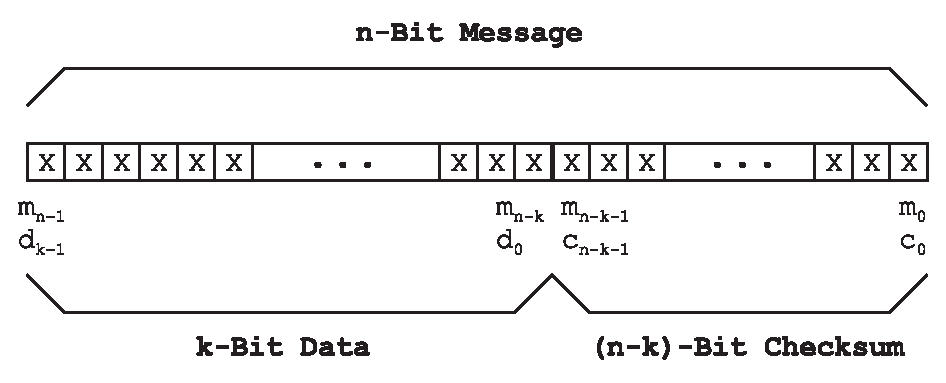
\includegraphics[width=4.6in]{c_edc0/cword02.eps}
\caption{Message Consisting Of The Concatenation Of $k$ Data Bits And $n-k$
         Check Bits, With Bit Notational Conventions For Cyclic Code Discusssion}
\label{fig:cedc0:scon0:sdpo0:01}
\end{figure}

A \index{cyclic code}\emph{cyclic code} is a linear code such that whenever
the vector $[m_0 \; m_1 \; m_2 \; \ldots{} \; m_{n-1}]$ is in the code, 
$[m_1 \; m_2 \; m_3 \; \ldots{} \; m_0]$ is also in the code.  When
this definition is applied recursively, it means that for any codeword, all
cyclic shifts of the codeword are also in the code (that is, in fact, why
a \emph{cyclic} code is called a \emph{cyclic} code).  For example, if 
10001 is a codeword; then 00011, 00110, 01100, and 11000 must also be
codewords (notice that these last four codewords are left cyclic shifts of the 
first codeword).  Note that since the code is linear, all sums of codewords 
must also be codewords.

A cyclic code is characterized by a generator polynomial, which we call
$g(x)$, of the form 

\begin{equation}
\label{eq:cedc0:scco0:sdpo0:01}
g(x) = g_{n-k} x_{n-k} + g_{n-k-1} x_{n-k-1} + \; \ldots \; + g_1 x + g_0,
\end{equation}

\noindent{}a polynomial of degree $n-k$, naturally containing up to $n-k+1$ terms.
Each coefficient $g_{n-k} \ldots g_{0}$ is chosen from $GF(2)$, so that
$g_{n-k} \ldots g_{0} \in \mathbb{B} = \{ 0 , 1 \}$.  We assume that
$g_{n-k}$ and $g_{0}$ are both 1.  We explain how the generator polynomial
specifies the code beginning in Section \ref{cedc0:scco0:ssut0}.

Cyclic codes are harnessed in two distinct ways, which we will call
the \emph{strong} and \emph{weak} ways.

In \emph{strong} utilization of cyclic codes
(Section \ref{cedc0:scco0:ssut0}), we must choose $g(x)$ in a very
special way with respect to $n$, and we cannot increase
$n$ arbitrarily (i.e. we are confined to messages of $n$ or
fewer bits).  If we choose $g(x)$ in this way, we can
control the minimum Hamming distance $\hat{d}$ of the cyclic code we specify.
We call this utilization \emph{strong} because we are able to preserve a 
strong property, the minimum Hamming distance $\hat{d}$ of the resulting code
(this is a very desirable feature, as it is in general not easy to construct a code
with a desirable large $\hat{d}$, and the theory of cyclic codes provides a way to do
this).
A typical ``strong'' utilization of a cyclic code may be in a communication peripheral
which can only accomodate a message of maximum length $\leq n$, and in this case
we can preserve strong properties of the cyclic code.

In \emph{weak} utilization of cyclic codes
(Section \ref{cedc0:scco0:swut0}), $n$ is unconstrained, and the minimum Hamming
distance of the code may degrade as far as $\hat{d}=2$ as $n$ is
increased.  We call such a utilization
\emph{weak} because only a \emph{weak} set of desirable properties can be preserved
in the resulting code.  A typical example of a weak utilization would be the CRC-32 (a
32-bit checksum) used to signature large files.  Such a utilization usually cannot
achieve even $\hat{d} = 3$, but can still preserve a low probability of undetected corruption
and protection against certain types of burst errors.

Note that the choice of generator polynomial $g(x)$ 
affects the properties of the code in both
the strong and weak utilizations, but in different ways.


%%%%%%%%%%%%%%%%%%%%%%%%%%%%%%%%%%%%%%%%%%%%%%%%%%%%%%%%%%%%%%%%%%%%%%%%%%%%%%%%
%%%%%%%%%%%%%%%%%%%%%%%%%%%%%%%%%%%%%%%%%%%%%%%%%%%%%%%%%%%%%%%%%%%%%%%%%%%%%%%%
%%%%%%%%%%%%%%%%%%%%%%%%%%%%%%%%%%%%%%%%%%%%%%%%%%%%%%%%%%%%%%%%%%%%%%%%%%%%%%%%
\subsection{\emph{Strong} Utilization Of Cyclic Codes}
%Subsection tag: sut0
\label{cedc0:scco0:ssut0}

In the strong utilization of a cyclic code,
the vector corresponding to the generator polynomial $g(x)$, 
$[0 \; \ldots \; 0 \; g_{n-k} \; g_{n-k-1} \; \ldots \; g_{0}]$ must 
be in the code, as must all of its cyclic shifts and sums of its
cyclic shifts.  A generator
matrix (not in standard form, and of course not the only generator 
matrix) for a cyclic code is of the form

\begin{equation}
\label{eq:cedc0:scco0:ssut0:02}
G = \left[
    \begin{array}{lllllllll}
    g_{n-k}  & g_{n-k-1}  & g_{n-k-2} &  \cdots  & g_{0}     &  0         &       0    &  \cdots{}  &   0 \\
    0        & g_{n-k}    & g_{n-k-1} &  \cdots  & g_{1}     &  g_{0}     &       0    &  \cdots{}  &   0 \\
    0        &   0        & g_{n-k}   &  \cdots  & g_{2}     &  g_{1}     &   g_{0}    &  \cdots{}  &   0 \\
    \vdots{} &            &           &          &           &            &            &            &     \\
    0        &   0        &   0       &  \cdots  &           &            &            &  \cdots{}  &   g_{0}   
    \end{array}
    \right]_{k \times n} \!\!\!\!\!\!\!\!\!\!.
\end{equation}

\noindent{}Note that the generator matrix in (\ref{eq:cedc0:scco0:ssut0:02})
has rows which are cyclic shifts of the coefficients of $g(x)$ (and 
for reasons discussed later, the other cyclic
shifts are also in the code).  Note also that $G$ is a
$k \times n$ matrix, consistent with (\ref{eq:cedc0:slco0:sgma0:01b}).

It is apparent from (\ref{eq:cedc0:scco0:ssut0:02}) that G can be
transformed into the form of (\ref{eq:cedc0:slco0:sgma0:01}) by
elementary row operations.  Two arguments can be
made.  First, by theorem, the determinant of an upper triangular matrix
(the first $k$ columns of $G$) is the product of the diagonal elements, 
and since we've assumed $g_0 = g_{n-k} = 1$, this determinant is necessarily 1.
Since the first $k$ columns of $G$ have full rank, they can be transformed
into $I_{k \times k}$.  Second, it is clear using elementary row operations how
to transform the first $k$ columns of $G$ into 
$I_{k \times k}$ (Exercise \ref{exe:cedc0:sexe0:03}).

\begin{vworkexamplestatement}
\label{ex:cedc0:scco0:ssut0:01}
For the $(7,4)$ code characterized by the generator polynomial 
$g(x) = 1 + x + x^3$, form the generator matrix of the code
as in (\ref{eq:cedc0:scco0:ssut0:02}), reduce it by elementary
row operations to the form of (\ref{eq:cedc0:slco0:sgma0:01}), 
and enumerate the $2^k = 16$ codewords.
\end{vworkexamplestatement}
\begin{vworkexampleparsection}{Solution}
With generator polynomial $g(x) = 1 + x + x^3$, $g_0 = 0$, $g_1 = 1$, 
$g_2 = 0$, and $g_3 = 1$.  By (\ref{eq:cedc0:scco0:ssut0:02}),

\begin{equation}
\label{eq:ex:cedc0:scco0:ssut0:01:01}
G = \left[
    \begin{array}{ccccccc}
    g_0 & g_1 & g_2 & g_3 &   0 &   0 &   0    \\
      0 & g_0 & g_1 & g_2 & g_3 &   0 &   0    \\
      0 &   0 & g_0 & g_1 & g_2 & g_3 &   0    \\
      0 &   0 &   0 & g_0 & g_1 & g_2 & g_3
    \end{array}
    \right] 
    =
    \left[
    \begin{array}{ccccccc}
      1 &   1 &   0 &   1 &   0 &   0 &   0    \\
      0 &   1 &   1 &   0 &   1 &   0 &   0    \\
      0 &   0 &   1 &   1 &   0 &   1 &   0    \\
      0 &   0 &   0 &   1 &   1 &   0 &   1
    \end{array}
    \right] .
\end{equation}

Adding (in the sense of $GF(2)$, see Section \ref{cedc0:sfft0:dff0})
the second row to the first yields

\begin{equation}
\label{eq:ex:cedc0:scco0:ssut0:01:02}
G = \left[
    \begin{array}{ccccccc}
      1 &   0 &   1 &   1 &   1 &   0 &   0    \\
      0 &   1 &   1 &   0 &   1 &   0 &   0    \\
      0 &   0 &   1 &   1 &   0 &   1 &   0    \\
      0 &   0 &   0 &   1 &   1 &   0 &   1
    \end{array}
    \right] .
\end{equation}

Adding the third row to the first row and to the second row (two
row operations) yields

\begin{equation}
\label{eq:ex:cedc0:scco0:ssut0:01:03}
G = \left[
    \begin{array}{ccccccc}
      1 &   0 &   0 &   0 &   1 &   1 &   0    \\
      0 &   1 &   0 &   1 &   1 &   1 &   0    \\
      0 &   0 &   1 &   1 &   0 &   1 &   0    \\
      0 &   0 &   0 &   1 &   1 &   0 &   1
    \end{array}
    \right] .
\end{equation}

Finally, adding the fourth row to the second row and to the third row (two
row operations) yields

\begin{equation}
\label{eq:ex:cedc0:scco0:ssut0:01:04}
G = \left[
    \begin{array}{ccccccc}
      1 &   0 &   0 &   0 &   1 &   1 &   0    \\
      0 &   1 &   0 &   0 &   0 &   1 &   1    \\
      0 &   0 &   1 &   0 &   1 &   1 &   1    \\
      0 &   0 &   0 &   1 &   1 &   0 &   1
    \end{array}
    \right] .
\end{equation}

The $2^4 = 16$ codewords can be enumerated by forming all linear combinations
of the rows of any of the matrices 
(\ref{eq:ex:cedc0:scco0:ssut0:01:01})
through (\ref{eq:ex:cedc0:scco0:ssut0:01:04}).  These 16 codewords are
enumerated in Table \ref{tbl:ex:cedc0:scco0:ssut0:01:01}.

\begin{table}
\caption{$2^4 = 16$ Codewords For Code Of Example \ref{ex:cedc0:scco0:ssut0:01}}
\label{tbl:ex:cedc0:scco0:ssut0:01:01}
\begin{center}
\begin{tabular}{|c|c|}
\hline
Data                      & Codeword  \\
(Value Of $k$ Data Bits)  &           \\
\hline
\hline
 0             &  0000 000 \\
\hline
 1             &  0001 101 \\
\hline
 2             &  0010 111 \\
\hline
 3             &  0011 010 \\
\hline
 4             &  0100 011 \\
\hline
 5             &  0101 110 \\
\hline
 6             &  0110 100 \\
\hline
 7             &  0111 001 \\
\hline
 8             &  1000 110 \\
\hline
 9             &  1001 011 \\
\hline
10             &  1010 001 \\
\hline
11             &  1011 100 \\
\hline
12             &  1100 101 \\
\hline
13             &  1101 000 \\
\hline
14             &  1110 010 \\
\hline
15             &  1111 111 \\
\hline
\end{tabular}
\end{center}
\end{table}
\end{vworkexampleparsection}
\vworkexamplefooter{}



%%%%%%%%%%%%%%%%%%%%%%%%%%%%%%%%%%%%%%%%%%%%%%%%%%%%%%%%%%%%%%%%%%%%%%%%%%%%%%%%
%%%%%%%%%%%%%%%%%%%%%%%%%%%%%%%%%%%%%%%%%%%%%%%%%%%%%%%%%%%%%%%%%%%%%%%%%%%%%%%%
%%%%%%%%%%%%%%%%%%%%%%%%%%%%%%%%%%%%%%%%%%%%%%%%%%%%%%%%%%%%%%%%%%%%%%%%%%%%%%%%
\subsection{\emph{Weak} Utilization Of Cyclic Codes}
%Subsection tag: wut0
\label{cedc0:scco0:swut0}


%%%%%%%%%%%%%%%%%%%%%%%%%%%%%%%%%%%%%%%%%%%%%%%%%%%%%%%%%%%%%%%%%%%%%%%%%%%%%%%%
%%%%%%%%%%%%%%%%%%%%%%%%%%%%%%%%%%%%%%%%%%%%%%%%%%%%%%%%%%%%%%%%%%%%%%%%%%%%%%%%
%%%%%%%%%%%%%%%%%%%%%%%%%%%%%%%%%%%%%%%%%%%%%%%%%%%%%%%%%%%%%%%%%%%%%%%%%%%%%%%%
\subsection{Perfect Codes}
%Subsection tag: pfc0
\label{cedc0:scob0:spfc0}

We define a \index{perfect code}\emph{perfect code} as a code 
where (\ref{eq:cedc0:scob0:rbc0:shsp0:01})
is an equality---that is, where the volume of the $2^k$ packing spheres precisely
consumes the $2^n$ messages available.  A perfect code has no ``waste'':  that is, 
there are no messages which do not participate in maintaining the required separation
between codewords.

In this section, we address two issues:

\begin{itemize}
\item The existence of integer solutions to

      \begin{equation}
      \label{eq:cedc0:scob0:spfc0:01}
      2^k V(n, \rho) = 2^n ,
      \end{equation}

      which is a question from number theory.

\item Given $n$,$k$ which satisfy (\ref{eq:cedc0:scob0:spfc0:01}), the existence
      of the codes whose possible existence is predicted.  It should be remembered
      that  (\ref{eq:cedc0:scob0:spfc0:01}) is a necessary but not sufficient 
      condition.
\end{itemize}


%%%%%%%%%%%%%%%%%%%%%%%%%%%%%%%%%%%%%%%%%%%%%%%%%%%%%%%%%%%%%%%%%%%%%%%%%%%%%%%%
%%%%%%%%%%%%%%%%%%%%%%%%%%%%%%%%%%%%%%%%%%%%%%%%%%%%%%%%%%%%%%%%%%%%%%%%%%%%%%%%
%%%%%%%%%%%%%%%%%%%%%%%%%%%%%%%%%%%%%%%%%%%%%%%%%%%%%%%%%%%%%%%%%%%%%%%%%%%%%%%%
\subsubsection[Existence Of Integer Solutions To 
               \protect\mbox{\protect$2^k V(n, \rho) = 2^n$}]
              {Existence Of Integer Solutions To 
               \protect\mbox{\protect\boldmath$2^k V(n, \rho) = 2^n$}}
%Subsubsection tag: pfc0
\label{cedc0:scob0:spfc0:seis0}



%%%%%%%%%%%%%%%%%%%%%%%%%%%%%%%%%%%%%%%%%%%%%%%%%%%%%%%%%%%%%%%%%%%%%%%%%%%%%%%%
%%%%%%%%%%%%%%%%%%%%%%%%%%%%%%%%%%%%%%%%%%%%%%%%%%%%%%%%%%%%%%%%%%%%%%%%%%%%%%%%
%%%%%%%%%%%%%%%%%%%%%%%%%%%%%%%%%%%%%%%%%%%%%%%%%%%%%%%%%%%%%%%%%%%%%%%%%%%%%%%%
\subsubsection{Existence Of Predicted Perfect Codes}
%Subsubsection tag: epc0
\label{cedc0:scob0:spfc0:sepc0}


%%%%%%%%%%%%%%%%%%%%%%%%%%%%%%%%%%%%%%%%%%%%%%%%%%%%%%%%%%%%%%%%%%%%%%%%%%%%%%%%
%%%%%%%%%%%%%%%%%%%%%%%%%%%%%%%%%%%%%%%%%%%%%%%%%%%%%%%%%%%%%%%%%%%%%%%%%%%%%%%%
%%%%%%%%%%%%%%%%%%%%%%%%%%%%%%%%%%%%%%%%%%%%%%%%%%%%%%%%%%%%%%%%%%%%%%%%%%%%%%%%
\section{Economical Implementation Of Linear Codes In Software}
%Section tag: eim0
\label{cedc0:seim0}


%%%%%%%%%%%%%%%%%%%%%%%%%%%%%%%%%%%%%%%%%%%%%%%%%%%%%%%%%%%%%%%%%%%%%%%%%%%%%%%%
%%%%%%%%%%%%%%%%%%%%%%%%%%%%%%%%%%%%%%%%%%%%%%%%%%%%%%%%%%%%%%%%%%%%%%%%%%%%%%%%
%%%%%%%%%%%%%%%%%%%%%%%%%%%%%%%%%%%%%%%%%%%%%%%%%%%%%%%%%%%%%%%%%%%%%%%%%%%%%%%%
\section[\protect\mbox{\protect$\hat{d}=2$} Codes Useful In Microcontroller Work]
        {\protect\mbox{\protect\boldmath$\hat{d}=2$} Codes Useful In Microcontroller Work}
%Section tag: dtc0
\label{cedc0:sdtc0}


%%%%%%%%%%%%%%%%%%%%%%%%%%%%%%%%%%%%%%%%%%%%%%%%%%%%%%%%%%%%%%%%%%%%%%%%%%%%%%%%
%%%%%%%%%%%%%%%%%%%%%%%%%%%%%%%%%%%%%%%%%%%%%%%%%%%%%%%%%%%%%%%%%%%%%%%%%%%%%%%%
%%%%%%%%%%%%%%%%%%%%%%%%%%%%%%%%%%%%%%%%%%%%%%%%%%%%%%%%%%%%%%%%%%%%%%%%%%%%%%%%
\section[\protect\mbox{\protect$\hat{d}=3$} Codes Useful In Microcontroller Work]
        {\protect\mbox{\protect\boldmath$\hat{d}=3$} Codes Useful In Microcontroller Work}
%Section tag: dhc0
\label{cedc0:sdhc0}



%%%%%%%%%%%%%%%%%%%%%%%%%%%%%%%%%%%%%%%%%%%%%%%%%%%%%%%%%%%%%%%%%%%%%%%%%%%%%%%%
%%%%%%%%%%%%%%%%%%%%%%%%%%%%%%%%%%%%%%%%%%%%%%%%%%%%%%%%%%%%%%%%%%%%%%%%%%%%%%%%
%%%%%%%%%%%%%%%%%%%%%%%%%%%%%%%%%%%%%%%%%%%%%%%%%%%%%%%%%%%%%%%%%%%%%%%%%%%%%%%%
\section{Acknowledgements}
\label{cedc0:sack0}

I'm very grateful to the following individuals who contributed insight
about error-detecting and error-correcting
codes on \index{comp.arch.embedded@\texttt{comp.arch.embedded}}\texttt{comp.arch.embedded}
and other
newsgroups:
Alan Coppola,
Eric Doenges,
Glen Herrmannsfeldt,
Dan Kotlow,
John Larkin,
Steven Murray,
Sphero Pefhany,
Jan-Hinnerk Reichert,
Thad Smith,
and
Jim Stewart.

I'm grateful to 
\index{Sperber, Ron}   Ron Sperber   \cite{bibref:i:ronsperber} and
\index{Chapman, Robin} Robin Chapman \cite{bibref:i:robinchapman}
for assistance with field theory offered on the 
\texttt{sci.math} newsgroup \cite{bibref:n:scimathnewsgroup}.

I'm also grateful to Mr. Michael J. Downes of the 
\index{comp.text.tex@\texttt{comp.text.tex}}\texttt{comp.text.tex} 
newsgroup, who assisted me with a technical difficulty involving
the \LaTeX ``$\backslash$\texttt{protect}'' command.


%%%%%%%%%%%%%%%%%%%%%%%%%%%%%%%%%%%%%%%%%%%%%%%%%%%%%%%%%%%%%%%%%%%%%%%%%%%%%%%%
%%%%%%%%%%%%%%%%%%%%%%%%%%%%%%%%%%%%%%%%%%%%%%%%%%%%%%%%%%%%%%%%%%%%%%%%%%%%%%%%
%%%%%%%%%%%%%%%%%%%%%%%%%%%%%%%%%%%%%%%%%%%%%%%%%%%%%%%%%%%%%%%%%%%%%%%%%%%%%%%%
\section{Exercises}
\label{cedc0:sexe0}

\begin{vworkexercisestatement}
\label{exe:cedc0:sexe0:01}
Show that the minimum Hamming distance of the code $\{0001, 0110, 1010, 1101\}$
is 2.
\end{vworkexercisestatement}

\begin{vworkexercisestatement}
\label{exe:cedc0:sexe0:02}
Verify Equation \ref{eq:cedc0:shco0:02}.
\end{vworkexercisestatement}

\begin{vworkexercisestatement}
\label{exe:cedc0:sexe0:03}
Outline a procedure for transforming the $G$ of 
(TBD%
%\ref{eq:cedc0:scco0:sdpo0:02}%
) into 
the form of (\ref{eq:cedc0:slco0:sgma0:01}).
\end{vworkexercisestatement}
\vworkexercisefooter{}

\vworkexercisefooter{}

%End of file c_edc0.tex



%Chapter:  Boolean Algebra And Simplification Of Boolean Functions
\chapter[\cbalzeroshorttitle{}]{\cbalzerolongtitle{}}

\label{cbal0}

\section{Introduction, Definition, And History Of Boolean Algebra}
%Section tag:  INT0
\label{cbal0:sint0}

\index{Boolean algebra}
In this chapter, we review methods of 
simplifying \index{Boolean function}Boolean functions, and
show how such methods can be used to simplify software constructs
or to construct software which is more compact (in ROM or RAM) 
or executes more quicky.

Boolean algebra is named after \index{Boole, George}George Boole, 
a 19th-century British mathematician.
A fairly concise biography of George Boole comes from 
\cite{bibref:w:georgeboolebio01}:

\begin{quote}
George Boole first attended a school in Lincoln, then a commerical school.
His early instruction in mathematics, however, was from his father who
also gave George a liking for constructing optical instruments.  George's
interests turned to languages and he received instruction in Latin from a 
local bookseller.

By the age of 12 George had become so skilled in Latin that it provoked
an argument.  He translated an ode by the Latin poet Horace which his 
father was so proud of that he had it published.  However the talent was
such that a local schoolmaster disputed that any 12 year old could
have written with such depth.

Boole did not study for an academic degree, but from the age of 16 he was an 
assistant school teacher.  He maintained his interest in languages
and intended to enter the Church.  From 1835, however, he seems to have
changed his mind for he opened his own school and began to study mathematics
on his own.  He was later to realize that he had almost wasted five years
in trying to teach himself the subject instead of having a skilled teacher.

At this time Boole studied the works of Laplace and Lagrange, making 
notes which would later be the basis for his first mathematics paper.
However he did receive encouragement from Duncan Gregory who at this 
time was in Cambridge and the editor of the recently founded
\emph{Cambridge Mathematical Journal}.

Boole was unable to take Duncan Gregory's advice and study courses at 
Cambridge as he required the income from his school to look after
his parents.  However he began publishing in the \emph{Cambridge 
Mathematical Journal} and his interests were also influenced by Duncan Gregory
as he began to study algebra. An application of algebraic methods 
to the solution of differential equations was published by Boole in the
\emph{Transactions of the Royal Society} and for this work he received 
the Society's Royal Medal.  His mathematical work was beginning to bring
him fame.

Boole was appointed to the chair of mathematics at Queens College, 
Cork in 1849. He taught there for the rest of his life, gaining a reputation
as an outstanding and dedicated teacher.

In 1854 he published \emph{An investigation into the Laws of Thought, on 
Which are founded the Mathematical Theories of Logic and Probabilities}.
Boole approached logic in a new way reducing it to a simple algebra, 
incorporating logic into mathematics.  He pointed out the analogy
between algebraic symbols and those that represent logical forms. 
It began the algebra of logic called Boolean algebra which now finds
application in computer construction, switching circuits etc.

Boole also worked on differential equations, the influential 
\emph{Treatise on Differential Equations} appeared in 1859, the calculus of finite
differences, \emph{Treatise on the Calculus of Finite Differences} (1860), 
and general methods in probability. He published around 50 papers and
was one of the first to investigate the basic properties of numbers, such 
as the distributive property, that underlie the subject of algebra.

Many honours were given to Boole as the genius in his work was recognised. 
He received honorary degrees from the universities of Dublin
and Oxford and was elected a Fellow of the Royal Society (1857). 
However his career, which was started rather late, came to an unfortunately
early end when he died at the age of 49.  The circumstances are described 
by Macfarlane in [17]\footnote{As reproduced from 
\cite{bibref:w:georgeboolebio01}---this is not a valid reference
number in this work.} as follows:

\begin{quote}
One day in 1864 he walked from his residence to the College, 
a distance of two miles, in the drenching rain, and lectured in wet
clothes.  The result was a feverish cold which soon fell upon his 
lungs and terminated his career \ldots{}
\end{quote}

What Macfarlane fails to say is that Boole's wife 
(Mary---niece of Sir George Everest, after whom the mountain is named) believed that a
remedy should resemble the cause. She put Boole to bed and threw 
buckets of water over the bed since his illness had been caused by getting
wet.

Hirst described Boole as:

\begin{quote}
\ldots{} evidently an earnest able and at the same time a genial man.
\end{quote}

His work was praised by \index{DeMorgan, Augustus}De Morgan who said:

\begin{quote}
Boole's system of logic is but one of many proofs of genius and patience combined.
\ldots{} That the symbolic processes of algebra,
invented as tools of numerical calculation, should be competent to 
express every act of thought, and to furnish the grammar and
dictionary of an all-containing system of logic, would not have 
been believed until it was proved. When Hobbes \ldots{} published his
``Computation or Logique'' he had a remote glimpse of some of the points which 
are placed in the light of day by Mr Boole.
\end{quote}

Boolean algebra has wide applications in telephone switching and the 
design of modern computers. Boole's work has to be seen as a
fundamental step in today's computer revolution.
(Article by: J. J. O'Connor and E. F. Robertson.)
\end{quote}

In the preface of
\cite{bibref:b:whitesittbooleanalgandapps}, Whitesitt explains the
significance of Boole's work:

\begin{quote}
George Boole (1815-1864) introduced in his book \emph{The Laws Of Thought}
the first systematic treatment of logic and developed for this purpose
the algebraic system now known by his name, Boolean algebra.  Few
mathematical works of the last 100 years have had a greater impact
upon mathematics and philosophy than this famous book.  The significance
of the work has been well expressed by Augustus De Morgan:

\begin{quote}
That the symbolic processes of algebra, invented as tools of numerical
calculation, should be competent to express every act of thought, and to
furnish the grammar and dictionary of an all-containing system of
logic, would not have been believed until it was proved in
\emph{Laws Of Thought}.
\end{quote}

In addition to its applications in the field of logic, Boolean algebra
has two other important applications.  The first of these arises from
the fact that Boolean algebra is the natural algebra with which to
treat the combination of sets of elements under the operations of
intersection and union of sets.  With the addition of the idea of
``number of elements'' in a set, Boolean algebra becomes the 
foundation for the theory of probability.  The algebra
of sets is also important in many other branches of mathematics.

With the publication of two papers approximately 20 years 
ago,\footnote{Whitesitt's book was first published in 1961,
so Whitesitt probably means \emph{20 years ago} with 
respect to 1961.}
\index{Shannon, Claude E.}Claude E. Shannon introduced a new 
area of application of
Boolean algebra when he showed that the basic properties of
series and parallel combinations of bistable electrical
devices such as relays could be adequately represented
by this algebra.  Since this time, Boolean algebra has
played a significant role in the important and complicated
task of designing telephone switching circuits, automatic
control devices, and electronic computers.  At the present
time, more interest is centered in this application than
in either of the others.
\end{quote}

Claude E. Shannon's classic 1937 thesis is described separately
in several places.  From \cite{{bibref:w:boolealghist01}}:

\begin{quote}
Shannon, whose 1937 thesis centered on the improvement of the 
Differential Analyzer, a clunky mechanical gear and shaft addition
machine, realized that Boolean algebraic principles governed its operation.
He proposed that such a machine could be built with circuits using 
components that were governed by Boolean principles.  Shannon's paper
was regarded as genius and his ideas were almost immediately
incorporated into the telephone system.  Shannon took a position at Bell
Labs.  Later, of course, Shannon's thesis came to be seen as a focal point
in the development of modern computers.
\end{quote}

In \cite{bibref:w:boolealghist02}, Shannon's thesis is described
very favorably:

\begin{quote}
Around the 1850's, the British mathematician George Boole was 
busily inventing a new form of mathematics, in which he represented
logical expressions in a mathematical form now known as
Boolean Algebra.

Unfortunately, with the exception of students of philosophy
and symbolic logic, Boolean Algebra was destined to remain 
largely unknown and unused for the better part of a century.
It fact it was not until 1938 that Claude E. Shannon published
an article based on his master's thesis at MIT.  (Shannon's
thesis has since been described as: \emph{``Possibly the
most important master's thesis of the twentieth century.''})

In his paper, which was widely circulated, Shannon showed how
Boole's concepts of TRUE and FALSE could be used to represent
the functions of switches in electronic circuits.  It is difficult
to convey just how important this concept was; suffice it to say
that Shannon had provided electronics engineers with the mathematical
tool they needed to design digital electronic circuits, and these 
techniques remain the cornerstone of digital electronic
design to this day.

Apropos of nothing at all, Shannon is also credited with the invention
of the rocket-powered Frisbee, and is famous for riding down the
corridors of Bell Laboratories on a unicycle while simultaneously
juggling four balls.
\end{quote}

In summary, in 1854 George Boole published his classic work 
\emph{An investigation into the Laws of Thought, on 
Which are founded the Mathematical Theories of Logic and Probabilities},
which laid the foundation of manipulation of 
logical ideas using algebraic mechanisms.  Boole's ideas 
were revived in 1937 and 1938 by Claude E. Shannon
in his master's thesis and a subsequent article, in which
Shannon applied Boole's ideas to the design of electric
switching circuits.  Shannon's reapplication of Boole's work
came to be seen as a focal point in the development of modern
computers.


\section[Simplification By Algebraic Manipulation]
        {Simplification Of Boolean Functions By Algebraic Manipulation}
%Section Tag: SAM0
\label{cbal0:ssam0}

We assume that the reader has had previous exposure to 
\index{Boolean function!simplification of}simplification of
Boolean functions.  For this reason, this section is a review (it is terse
and moves quickly).  (For readers without this background, we
recommend \cite{bibref:b:manodigitaldesignseconded}.)

The most direct way to simplify Boolean functions is 
\index{Boolean function!algebraic simplification}\emph{algebraic}
transformation---to use transformation postulates and 
theorems to transform algebraic
expressions to a more desirable equivalent form.


\subsection{Nomenclature And Operators}
%Subsection Tag:  NOM0
\label{cbal0:ssam0:snom0}

We define the set of two elements which we will use in 
two-valued Boolean
algebra as `0' and '1' (or alternatively as 
`FALSE' and `TRUE', respectively).
All functions which we will describe subsequently require
inputs which are members of this set and will produce outputs
which are also members of this set.

The \emph{complement} or \emph{negation} operator (or function)
maps from 0$\rightarrow$1 and from 1$\rightarrow$0 (see Table 
\ref{tbl:cbal0:ssam0:snom0:01}).
We denote this operator
by an apostrophe
following the variable to be complemented (example: $x'$).
Alternatively, in some circumstances, we may use the
tilde ($\sim{}x$), the overbar ($\overline{x}$), or
the negation symbol ($\neg{}x$).

\begin{table}
\caption{Definition Of Logical Complement, Logical And, Logical Or, And Logical 
         Exclusive Or Operators}
\label{tbl:cbal0:ssam0:snom0:01}
\begin{center}
\begin{tabular}{|c|c||c|c|c|c|}
\hline
$X$ & $Y$  & $X'$ & $XY$ & $X+Y$ & $X \oplus{} Y$ \\
\hline
\hline
 0 & 0 & 1 & 0 & 0 & 0 \\
\hline
 0 & 1 & 1 & 0 & 1 & 1 \\
\hline
 1 & 0 & 0 & 0 & 1 & 1 \\
\hline
 1 & 1 & 0 & 1 & 1 & 0 \\
\hline
\end{tabular}
\end{center}
\end{table}

The \emph{logical AND} (or simply \index{AND}\index{Boolean algebra!AND}\emph{AND}) 
operator (or function)
returns TRUE if both of its input arguments are TRUE 
(see Table 
\ref{tbl:cbal0:ssam0:snom0:01}).
We denote this operator
by the \emph{times} symbol (example: $x \times{} y$), by
the keyword `AND', or by placing the operands adjacent to
each other (examples: $xy$, $x(y)$).

The \emph{logical OR}
(or simply \index{OR}\index{Boolean algebra!OR}\emph{OR}) 
operator (or function)
returns TRUE if either of its input arguments are TRUE 
(see Table 
\ref{tbl:cbal0:ssam0:snom0:01}).
We denote this operator
by the \emph{plus} symbol (example: $x + y$)  or by
the keyword `OR'.

The \emph{logical exclusive-OR}
(or simply \index{XOR}\index{Boolean algebra!XOR} \emph{XOR})
operator (or function)
returns TRUE if either but not both of its input arguments are TRUE 
(see Table 
\ref{tbl:cbal0:ssam0:snom0:01}).
We denote this operator
by the \emph{circled plus} symbol (example: $x \oplus{} y$),
by the \emph{caret} character (example: $x$\^{}$y$),  or by
the keyword `XOR'.

The exclusive-OR function is not a
function traditionally considered in the canonical forms of Boolean
algebra.  However, we consider it here because our aims may in
some cases be subtly
different than the aims of classic two-valued Boolean algebra.
The goal of classic Boolean algebra is to minimize the number of
terms which appear in a canonical form.
However, often our goal here is to rearrange Boolean functions into a form
which is optimal for implementation on a computer.  Since actual
computers usually provide a bitwise exclusive-OR instruction, there
are some applications where it may be useful to consider the
underlying instruction set of the computer (for example,
see \emph{Vertical Counters},
Section \ref{cbal0:svct0}).

In general, there are $2^{2^N}$ different Boolean functions of $N$
input variables, so it isn't practical to name functions involving more
than 2 input variables.  There are 16 ($=2^{2^2}$) Boolean functions of
2 input variables, and these are enumerated in
Table \ref{tbl:cbal0:ssam0:snom0:02}.

\begin{table}
\caption{Sixteen Possible Boolean Functions $f(A,B)$ Of Two Boolean Variables}
\label{tbl:cbal0:ssam0:snom0:02}
\begin{center}
\begin{tabular}{|c||c|c|c|c||l|}
\hline
\small{Func.} & $\scriptstyle{f(1,1)}$ & $\scriptstyle{f(1,0)}$ 
              & $\scriptstyle{f(0,1)}$ & $\scriptstyle{f(0,0)}$ 
			  & Function Description \\
\small{Num.}  &          &          &          &          &                 \\
\hline
\hline
 0 & 0 & 0 & 0 & 0 & \small{``Zero'' or  ``clear'' function.  Always}       \\
   &   &   &   &   & \small{returns zero regardless of $A$ and $B$  }       \\
   &   &   &   &   & \small{input values.                           }       \\
\hline
 1 & 0 & 0 & 0 & 1 & \small{Logical NOR = $(A+B)'$.                 }       \\
\hline
 2 & 0 & 0 & 1 & 0 & \small{Inhibition = $BA'$.  So named because   }       \\
   &   &   &   &   & \small{a TRUE value of $A$ inhibits $B$.  Also }       \\
   &   &   &   &   & \small{equivalent to $B>A$ or to $A<B$.        }       \\
\hline
 3 & 0 & 0 & 1 & 1 & \small{NOT A = $A'$.  Ignores $B$ and returns  }       \\
   &   &   &   &   & \small{$A'$.                                   }       \\
\hline
 4 & 0 & 1 & 0 & 0 & \small{Inhibition = $AB'$.  So named because   }       \\
   &   &   &   &   & \small{a TRUE value of $B$ inhibits $A$.  Also }       \\
   &   &   &   &   & \small{equivalent to $A>B$ or to $B<A$.        }       \\
\hline
 5 & 0 & 1 & 0 & 1 & \small{NOT B = $B'$.  Ignores $A$ and returns  }       \\
   &   &   &   &   & \small{$B'$.                                   }       \\
\hline
 6 & 0 & 1 & 1 & 0 & \small{Exclusive-OR (XOR) = $A \oplus B$.  Also}       \\
   &   &   &   &   & \small{equivalent to $A \neq B$.               }       \\
\hline
 7 & 0 & 1 & 1 & 1 & \small{Logical NAND = $(AB)'$.                 }       \\
\hline
 8 & 1 & 0 & 0 & 0 & \small{Logical AND = $AB$.                     }       \\
\hline
 9 & 1 & 0 & 0 & 1 & \small{Equivalence:  true if $A=B$.  Also}       \\
   &   &   &   &   & \small{known as exclusive-NOR, i.e. $(A \oplus B)'$.}       \\
\hline
10 & 1 & 0 & 1 & 0 & \small{Copy $B$.  Ignores $A$ and returns $B$. }       \\
\hline
11 & 1 & 0 & 1 & 1 & \small{Implication:  $B \rightarrow A$ (if $B$ }       \\
   &   &   &   &   & \small{then $A$).  Also equivalent to $B \geq A$.}     \\
\hline
12 & 1 & 1 & 0 & 0 & \small{Copy $A$.  Ignores $B$ and returns $A$. }       \\
\hline
13 & 1 & 1 & 0 & 1 & \small{Implication:  $A \rightarrow B$ (if $A$ }       \\
   &   &   &   &   & \small{then $B$).  Also equivalent to $A \geq B$.}     \\
\hline
14 & 1 & 1 & 1 & 0 & \small{Logical OR = $A+B$.                     }       \\
\hline
15 & 1 & 1 & 1 & 1 & \small{``One'' or ``set'' function.  Always    }       \\
   &   &   &   &   & \small{returns one regardless of $A$ and $B$   }       \\
   &   &   &   &   & \small{input values.                           }       \\
\hline
\end{tabular}
\end{center}
\end{table}

\emph{Any} Boolean function can be synthesized using AND gates and inverters
(i.e. NOT gates), OR gates and inverters, NAND gates alone, or NOR 
gates alone.  However, not all Boolean functions can be synthesized
using AND gates alone or OR gates alone.


\subsection{Postulates And Theorems}
%Subsection Tag:  POS0
\label{cbal0:ssam0:spos0}

Mathematicians tend to be very picky about what exactly a
\emph{postulate} is versus what a \emph{theorem} is.  We are
far less picky.  Either one (a postulate or a theorem) is a
rule that can be used to transform a Boolean algebraic expression
into another expression which is equivalent but for one reason or another
more desirable.  For our purposes here, postulates and theorems
are interchangeable.

Table \ref{tbl:cbal0:ssam0:spos0:01} 
(from \cite{bibref:b:manodigitaldesignseconded}) 
supplies the important postulates and theorems which are useful in
algebraically simplifying Boolean functions.

In Table \ref{tbl:cbal0:ssam0:spos0:01}, we should explain what 
is meant by the \emph{Dual Postulate Or Theorem}.  To
quote \cite{bibref:b:manodigitaldesignseconded}, p. 41:

\begin{quote}
\ldots This important property of Boolean algebra is called
the \index{Boolean algebra!duality principle}\index{duality principle}%
\emph{duality principle}.
It states that every algebraic expression deducible from the postulates
of Boolean algebra remains valid if the operators and identity
elements are interchanged.  In a two-valued Boolean algebra,
the identity elements and the elements of the set $B$ are the
same:  1 and 0.  The duality principle has many applications.
If the \emph{dual} of an algebraic expression is desired, we
simply interchange OR and AND operators and replaces 1s by
0s and 0s by 1s.
\end{quote}

\begin{table}
\caption{Important Postulates And Theorems Of Two-Valued Boolean Algebra}
\label{tbl:cbal0:ssam0:spos0:01}
\begin{center}
\begin{tabular}{|c||c|c||l|}
\hline
\small{Postulate} &  \small{Postulate}   & \small{Dual}        & \small{Remarks}   \\
\small{Or}        &  \small{Or}          & \small{Postulate}   &                   \\
\small{Theorem}   &  \small{Theorem}     & \small{Or}          &                   \\
\small{Number}    &                      & \small{Theorem}     &                   \\
\hline
      1           &  $x + 0 = x$         & $x \cdot 1 = 1$     &                   \\
\hline
      2           &  $x + x' = 1$        & $x \cdot x' = 0$    &                   \\
\hline
      3           &  $x + x = x$         & $x \cdot x = x$     &                   \\
\hline
      4           &  $x + 1 = 1$         & $x \cdot 0 = 0$     &                   \\
\hline
      5           &  $(x')' = x$         &                     & \small{Involution.} \\
\hline
      6           &  $x + y = y + x$     & $x \cdot y = y \cdot x $ & \small{Commutative property.} \\
\hline
      7           &  $x + (y + z)$       & $x(yz) = (xy)z$  & \small{Associative property.} \\
                  &  $= (x + y) + z$     &                     &                            \\
\hline
      8           &  $x (y + z)$         & $x + yz$          & \small{Distributive property.} \\
                  &  $= xy + xz$                    & $= (x+y)(x+z)$      &                                \\
\hline
      9           &  $(x+y)' = x'y'$      & $(xy)' = x' + y'$  & \small{DeMorgan's theorem.} \\
\hline
     10           &  $x + xy = x$         & $x(x+y) = x$       & \small{Absorption.} \\
\hline
\end{tabular}
\end{center}
\end{table}

Note also from Item 8 of
Table \ref{tbl:cbal0:ssam0:spos0:01} that in Boolean algebra
AND distributes over OR and OR distributes over AND (waiting on
newsgroup posters to clarify).  This is unlike ``normal'' algebra, where 
in general,

\begin{equation}
x + yz \neq (x+y) (x+z).
\end{equation}

The \index{Boolean algebra!operator precedence}%
\index{operator precedence!Boolean algebra}\index{operator precedence}%
operator precedence for evaluating Boolean expressions assumed throughout
this work is:

\begin{quote}
\begin{enumerate}
\item Parenthesis.
\item NOT.
\item AND.
\item OR.
\end{enumerate}
\end{quote}

\noindent{}Note that this operator precedence very closely mirrors
the standard precedence of normal algebraic expressions.

\subsection{Canonical And Standard Forms}
%Subsection Tag:  CAS0
\label{cbal0:ssam0:scas0}

\cite{bibref:b:manodigitaldesignseconded}, p. 49 provides an concise and
excellent definition of \emph{minterms} and \emph{maxterms}.  The definition
here is taken primarily from that source.

A binary variable may appear either in its normal form ($x$, for example)
or in its complemented form ($x'$, for example).  Now consider two
binary variables $x$ and $y$ combined with an AND
operation.  Since each variable may appear in either form, there are four
possible combinations:  $x'y'$, $x'y$, $xy'$, and $xy$.  These
four AND terms are mutually exclusive and mutually exhaustive---that is,
no combination of values for
$x$ and
$y$ that causes one of these AND terms to be TRUE may cause any of the
others to be TRUE, and every combination of $x$ and $y$ will cause exactly
one of these AND terms to be TRUE.  Each of these
four AND terms is called a \index{Boolean algebra!minterm}\index{minterm}\emph{minterm}
or \index{Boolean algebra!standard product}\index{standard product}\emph{standard product}.
In a similar manner, $n$ variables can be combined to form $2^n$ minterms.

In a similar fashion, $n$ variables forming an OR term, with each variable 
being primed or unprimed, provide $2^n$ possible combinations, called
\index{Boolean algebra!maxterm}\index{maxterm}\emph{maxterms}, or
\index{Boolean algebra!standard sum}\index{standard sum}\emph{standard sums}.

\begin{table}
\caption{Minterms And Maxterms Of Three Boolean Variables}
\label{tbl:cbal0:ssam0:scas0:01}
\begin{center}
\begin{tabular}{|c|c|c||c|c||c|c|}
\hline
 $x$ & $y$ & $z$ & \small{Minterm} &  \small{Minterm}     & \small{Maxterm} & \small{Maxterm}     \\
     &     &     & \small{Term}    &  \small{Designation} & \small{Term}    & \small{Designation} \\
\hline
  0  &  0  &  0  & $x'y'z'$        &  $m_0$               & $x+y+z$         & $M_0$               \\
\hline
  0  &  0  &  1  & $x'y'z$         &  $m_1$               & $x+y+z'$        & $M_1$               \\
\hline
  0  &  1  &  0  & $x'yz'$         &  $m_2$               & $x+y'+z$        & $M_2$               \\
\hline
  0  &  1  &  1  & $x'yz$          &  $m_3$               & $x+y'+z'$       & $M_3$               \\
\hline
  1  &  0  &  0  & $xy'z'$         &  $m_4$               & $x'+y+z$        & $M_4$               \\
\hline
  0  &  0  &  1  & $x'y'z$         &  $m_5$               & $x+y+z'$        & $M_5$               \\
\hline
  1  &  1  &  0  & $xyz'$          &  $m_6$               & $x'+y'+z$       & $M_6$               \\
\hline
  1  &  1  &  1  & $xyz$           &  $m_7$               & $x'+y'+z'$      & $M_7$               \\
\hline
\end{tabular}
\end{center}
\end{table}

The two primary canonical forms in Boolean algebra are the
\emph{sum of minterms} (or \emph{sum of products}) form and the
\emph{product of maxterms} (or \emph{product of sums}) form.

The sum of minterms canonical form (which is the most common
canonical form) is sometimes written using a shorthand 
notation involving the Greek letter sigma ($\Sigma$).  We describe this
shorthand form now.  Consider the Boolean function of 3 variables,

\begin{equation}
\label{eq:cbal0:ssam0:scas0:01}
F(A, B, C) = A + B'C.
\end{equation}

\noindent{}Using the postulates and theorems in Table 
\ref{tbl:cbal0:ssam0:spos0:01}, it is possible
to expand (\ref{eq:cbal0:ssam0:scas0:01}) into
a sum of minterms form:

\begin{eqnarray}
\label{eq:cbal0:ssam0:scas0:02}
F(A, B, C) & = & A'B'C + AB'C' + AB'C + ABC' + ABC \\
           & = & m_1 m_4 m_5 m_6 m_7.\nonumber
\end{eqnarray}

\noindent{}(\ref{eq:cbal0:ssam0:scas0:02}) is also commonly written
in the shorthand form:

\begin{equation}
\label{eq:cbal0:ssam0:scas0:03}
F(A, B, C) = \Sigma{}(1, 4, 5, 6, 7).
\end{equation}

\noindent{}In the right-hand side of
(\ref{eq:cbal0:ssam0:scas0:03}), each integer
(1, 4, 5, 6, or 7) corresponds to the integer
that would be formed by treating the corresponding
minterm in (\ref{eq:cbal0:ssam0:scas0:02}) as
a binary number, i.e. $A=2^2$, $B=2^1$, and
$C=2^0$.  This is the basis of the short hand
notation.

A second but much less commonly used canonical form
is the product of maxterms (or product of sums) form,
which uses the Greek letter pi ($\Pi$) for its shorthand
form.  Without further explanation, we present the 
product of maxterms form of $\Sigma{}(1,4,5,6,7)$
(Eqns. \ref{eq:cbal0:ssam0:scas0:01} through
\ref{eq:cbal0:ssam0:scas0:03}) as
(\ref{eq:cbal0:ssam0:scas0:04}) 
through (\ref{eq:cbal0:ssam0:scas0:07}) 
(Figure \ref{fig:cbal0:ssam0:scas0:01}).

\begin{figure}
\begin{eqnarray}
\label{eq:cbal0:ssam0:scas0:04}
F(A, B, C) & = & \Sigma{}(1, 4, 5, 6, 7) \\
\label{eq:cbal0:ssam0:scas0:05}
           & = & \Pi{}(0, 2, 3)          \\
\label{eq:cbal0:ssam0:scas0:06}
		   & = & M_0 M_2 M_3             \\
\label{eq:cbal0:ssam0:scas0:07}
		   & = & (x+y+z)(x+y'+z)(x+y'+z')
\end{eqnarray}
\caption{Product Of Maxterms Form Of $\Sigma{}(1,4,5,6,7)$}
\label{fig:cbal0:ssam0:scas0:01}
\end{figure}


Because there are so many excellent digital logic books on the market
that contain examples and exercises of algebraic simplification
(we recommend \cite{bibref:b:manodigitaldesignseconded}), we don't
dwell on algebraic simplification or provide examples.  Again, we
assume that nearly all of our readers have had a course in digital
logic or symbolic logic.


\section[Karnaugh Maps]
        {Simplification Of Boolean Functions Using Karnaugh Maps}
%Section tag:  SKM0
\label{cbal0:skm0}

In 1953, M. Karnaugh published the graphical map method of simplifying
combinational logic functions (\cite{bibref:p:kmapclassic01}).  This
method has come to be known as the \emph{Karnaugh map} or \emph{K-map}
method of reduction, and is taught to engineers in nearly every
digital logic class.

Although it is possible, starting from an arbitrary Boolean formula, to simplify
the formula through algebraic manipulation, algebraic simplification
has the disadvantage that formulas can have many forms and there is not
an easily remembered, precise, and repeatable procedure for algebraic simplification.
The Karnaugh map method has the advantage that each Boolean function
has only one graphical representation, and that the procedure for simplification
is simple and easily remembered.

In a Karnaugh map, each square corresponds to a possible minterm of the function.
The essence of the method is to populate a grid of squares with outputs of
the function to be simplified.  Each minterm that must exist in the
function (i.e. each combination of inputs for which the function
must return TRUE) receives a `1' in the corresponding square.  Each
combination of inputs for which the function must return FALSE
receives a `0' in the corresponding square.  Each combination of inputs
for which the function may return either TRUE or FALSE receives an
`X' in the corresponding square.

After the Karnaugh map squares are populated with 1's, 0's, and X's
corresponding to the required values of the function for each combination
of inputs, the 1's are graphically combined into the largest rectangle possible.
Each rectangle may include 1's, may include X's where convenient, but
may not include 0's.
Each of these squares is then translated into a product of uncomplemented and
complemented input variables, and these products are summed to
produce the simplified algebraic expression for the function.  (We don't 
belabor this process, because we assume that most of our readers
understand it very thoroughly.)  There are some subtle points
to the process, such as combining corners and the ``folding'' of the
5- and 6-variable maps, but we don't explain these subtle points here
because they are so thoroughly explained in so many books.

Figures \ref{fig:cbal0:skm0:00} through \ref{fig:cbal0:skm0:04}
supply the canonical forms of two-, three-, four-, five-, and
six-variable Karnaugh maps.

\begin{figure}
\centering
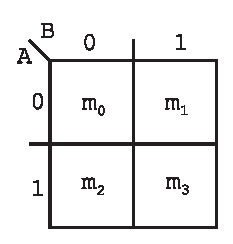
\includegraphics[width=1.25in]{c_bal0/kmap02cf.eps}
\caption{Canonical Form Of Two-Variable Karnaugh Map}
\label{fig:cbal0:skm0:00}
\end{figure}

\begin{figure}
\centering
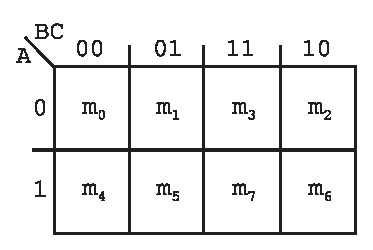
\includegraphics[height=1.25in]{c_bal0/kmap03cf.eps}
\caption{Canonical Form Of Three-Variable Karnaugh Map}
\label{fig:cbal0:skm0:01}
\end{figure}

\begin{figure}
\centering
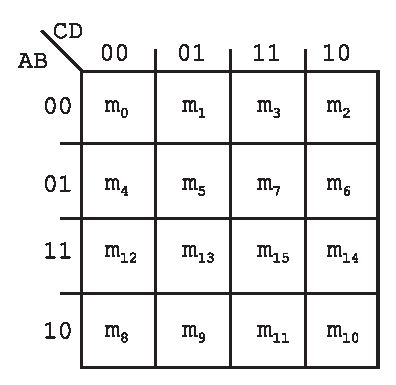
\includegraphics[height=2.0in]{c_bal0/kmap04cf.eps}
\caption{Canonical Form Of Four-Variable Karnaugh Map}
\label{fig:cbal0:skm0:02}
\end{figure}

\begin{figure}
\centering
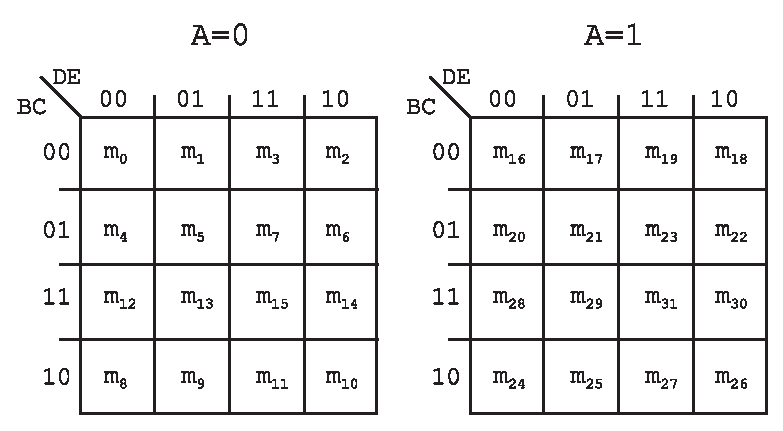
\includegraphics[width=4.25in]{c_bal0/kmap05cf.eps}
\caption{Canonical Form Of Five-Variable Karnaugh Map}
\label{fig:cbal0:skm0:03}
\end{figure}

\begin{figure}
\centering
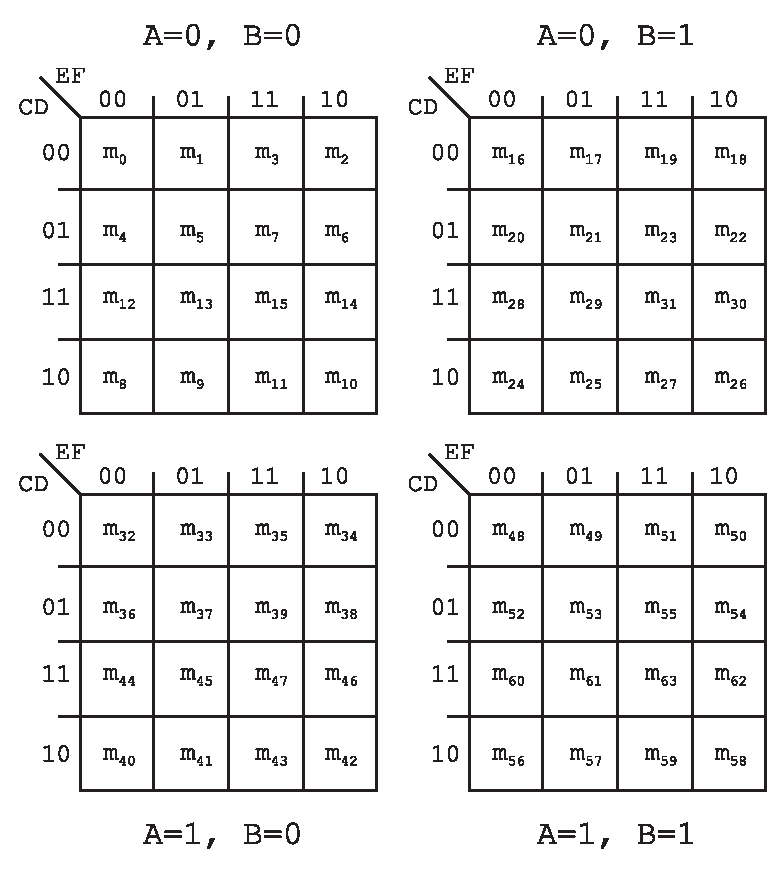
\includegraphics[width=4.5in]{c_bal0/kmap06cf.eps}
\caption{Canonical Form Of Six-Variable Karnaugh Map}
\label{fig:cbal0:skm0:04}
\end{figure}

\section[Simplification Using The Scheinman Method]
        {Simplification Of Boolean Functions Using The Scheinman Method}
%Section Tag: SCM0
\label{cbal0:sscm0}

Two major disadvantages of the Karnaugh map method of simplifying Boolean
functions are that:

\begin{itemize}
\item It is generally not possible to apply the method to functions
      of more than six variables.
\item It is not easy to automate the method (in the form that it is stated)
      because it is inherently graphical.
\end{itemize}

In 1962, A. H. Scheinman published a method for the simplification
of Boolean functions (\cite{bibref:p:scheinmanclassic01}) which is more amenable
to automation than the Karnaugh map method.

\section[The Quine-McCluskey Method]
        {Simplification Of Boolean Functions Using The Quine-McCluskey Method}


\section{Multiple Functions Of $N$ Boolean Variables}

Need to get back to Dr. Singh to inquire about the multiple Scheinman method.

\section{Vertical Counters}
%Section Tag: VCT0.
\label{cbal0:svct0}

\index{vertical counter}As has been hinted at elsewhere 
in this work, the need to generate
firmware which minimizes ROM consumption leads to clever (but perhaps
less-than-intuitive) programming techniques.  One such technique
is the construction of \emph{vertical counters}.  

A \index{vertical counter}vertical counter
is a set of identical combinational mappings or state machines 
where the inputs, state vector, intermediate results, and outputs of each
combinational mapping or state machine are stored as a single bit 
in the same position 
in each of multiple bytes or words.  When inputs, state vectors,
intermediate results, and outputs are stored
in this way, the bitwise logical instructions of the machine
(AND, OR, NOT, XOR) can be used to process several state machines in
parallel.  Vertical counters are intimately related to the reduction
of Boolean functions because such reduction must be performed in order
to design the vertical counter.  Debouncing and filtering, where the 
inputs and outputs naturally tend to be arranged as groups of bits,
are the most common application of vertical counters.

A very helpful resource on the web is the set of web pages 
maintained by \index{Dattalo, Scott}Scott Dattalo 
\cite{bibref:i:scottdattalo} for the
PIC microcontroller, including
especially \cite{bibref:w:sdattalovc02}.  Many of the vertical counter
designs which follow come from Mr. Dattalo's pages.

We abuse the term \emph{counter} somewhat, and we refer to 
any bit-wise mapping useful in microcontroller work as
a vertical counter.  We categorize vertical counters as 
\index{vertical counter!combinational}\emph{combinational}
(not truly a counter---the output is a function of the
inputs only), \index{vertical counter!sequential}\emph{sequential}
(the next state and output may be functions of both the
inputs and the present state---i.e. a proper state machine),
\index{vertical counter!cyclic}\emph{cyclic} (the counter
goes through a series of states and then repeats), or
\index{vertical counter!terminating} (the counter 
will reach a terminal state).

\subsection{2-Bit 4-State Cyclic Vertical Counter}
%Subsection Tag: TBF0
\label{cbal0:svct0:stbf0}
In this discussion of vertical counters, we begin with the simplest
designs, as often the simpler designs appear as part of more complex
designs.

Table \ref{tbl:cbal0:svct0:stbf0:01} supplies the state transition table 
for a 2-bit 4-state
cyclic vertical counter.  Note that the counter advances through the
bit patterns in the ``proper'' binary integer order.

\begin{table}
\caption{State Transition Table Of 2-Bit 4-State Cyclic Vertical Counter}
\label{tbl:cbal0:svct0:stbf0:01}
\begin{center}
\begin{tabular}{|c|c|c|c|}
\hline
 $A_k$     & $B_k$     & $A_{k+1}$ & $B_{k+1}$ \\
\hline
\hline
 0         & 0         & 0         & 1         \\
\hline
 0         & 1         & 1         & 0         \\
\hline
 1         & 0         & 1         & 1         \\
\hline
 1         & 1         & 0         & 0         \\
\hline
\end{tabular}
\end{center}
\end{table}

From Table \ref{tbl:cbal0:svct0:stbf0:01} it can be readily verified
even without a Karnaugh map that the least significant bit
($B$) is always complemented from one state to the next, so that
$B_{k+1} = \neg B_k$.  It can also be seen that the most significant
bit ($A$) is complemented from one state to the next only if $B$=1,
so that $A_{k+1} = A_k \oplus B_k$.

The implementation of such a counter in `C' comes immediately, since
`C' directly supports bit-wise complementation and exclusive-OR of
integers:

\begin{verbatim}
         A = A ^ B;
         B = ~B;
\end{verbatim}

Note in the `C' snippet above, the two operations are ordered so as
not to interfere with each other.  Note that reversing the two steps above
would not yield the desired result.


\subsection{3-Bit 8-State Cyclic Vertical Counter}
%Subsection Tag: TBF4
\label{cbal0:svct0:stbf4}


\subsection[$N$-Bit $2^N$-State Cyclic Vertical Counter]
           {\mbox{\boldmath $N$}-Bit \mbox{\boldmath $2^N$}-State Cyclic Vertical Counter}
%Subsection Tag: TBF1
\label{cbal0:svct0:stbf1}

The design of the 2-bit 4-state vertical counter presented in
Section \ref{cbal0:svct0:stbf0} (immediately above) and be
generalized to an $N$-bit $2^N$-state counter which follows
the traditional binary integer counting sequence.

Note from Section \ref{cbal0:svct0:stbf0} that the least
significant bit of the counter is always complemented
in going from one state to the next, and that each more
significant bit is complemented only if all less significant 
bits are 1.  If $X_0$ is the least significant bit of the 
counter and $X_N$ the most significant bit,
(\ref{eq:cbal0:svct0:stbf1:01}) through (\ref{eq:cbal0:svct0:stbf1:05})
(Figure \ref{eq:cbal0:svct0:stbf1:01})
describe how the counter is advanced from one state to the next.
Note that this set of equations gives only a \emph{logical} description
of how to obtain the next state from the present state---these
equations cannot be used as a direct blueprint for implementation because
earlier steps would destroy the results needed for later steps.

\begin{figure}
\begin{eqnarray}
\label{eq:cbal0:svct0:stbf1:01}
  X_0(k+1) & = & \neg X_0(k)                             \\
\label{eq:cbal0:svct0:stbf1:02}
  X_1(k+1) & = & X_1(k) \oplus X_0(k)                    \\ 
\label{eq:cbal0:svct0:stbf1:03}
  X_2(k+1) & = & X_2(k) \oplus (X_1(k) X_0(k))           \\
\label{eq:cbal0:svct0:stbf1:04}
  X_3(k+1) & = & X_3(k) \oplus (X_2(k) X_1(k) X_0(k))    \\
           & \ldots & \nonumber                          \\
\label{eq:cbal0:svct0:stbf1:05}
  X_N(k+1) & = & X_N(k) \oplus (X_{N-1}(k) \ldots X_0(k))
\end{eqnarray}
\caption{State Transition Equations Of $N$-Bit $2^N$-State Cyclic Vertical Counter}
\label{fig:cbal0:svct0:stbf1:01}
\end{figure}

The form of 
(\ref{eq:cbal0:svct0:stbf1:01}) through (\ref{eq:cbal0:svct0:stbf1:05})
suggests a way to economically implement an $N$-bit $2^N$-state
cyclic vertical counter in software, using two temporary
variables $TEMP_A$ and $TEMP_B$.  The general blueprint for
implementation is supplied as
(\ref{eq:cbal0:svct0:stbf1:06}) through (\ref{eq:cbal0:svct0:stbf1:20})
(Figure \ref{eq:cbal0:svct0:stbf1:02}).

\begin{figure}
\begin{eqnarray}
\label{eq:cbal0:svct0:stbf1:06}
  TEMP_A   & = & X_0                                     \\
\label{eq:cbal0:svct0:stbf1:07}
  X_0      & = & \neg X_0                                \\
\label{eq:cbal0:svct0:stbf1:08}
  TEMP_B   & = & X_1 TEMP_A                              \\
\label{eq:cbal0:svct0:stbf1:09}
  X_1      & = & X_1 \oplus TEMP_A                       \\ 
\label{eq:cbal0:svct0:stbf1:10}
  TEMP_A   & = & TEMP_B                                  \\
\label{eq:cbal0:svct0:stbf1:11}
  TEMP_B   & = & X_2 TEMP_B                              \\
\label{eq:cbal0:svct0:stbf1:12}
  X_2      & = & X_2 \oplus TEMP_A                       \\
\label{eq:cbal0:svct0:stbf1:13}
  TEMP_A   & = & TEMP_B                                  \\
\label{eq:cbal0:svct0:stbf1:14}
  TEMP_B   & = & X_3 TEMP_B                              \\
\label{eq:cbal0:svct0:stbf1:15}
  X_3      & = & X_3 \oplus TEMP_A                       \\
           & \ldots & \nonumber                          \\
\label{eq:cbal0:svct0:stbf1:16}
  X_{N-2}  & = & X_{N-2} \oplus TEMP_A                   \\
\label{eq:cbal0:svct0:stbf1:17}
  TEMP_A   & = & TEMP_B                                  \\
\label{eq:cbal0:svct0:stbf1:18}
  TEMP_B   & = & X_{N-1} TEMP_B                          \\
\label{eq:cbal0:svct0:stbf1:19}
  X_{N-1}  & = & X_{N-1} \oplus TEMP_A                   \\
\label{eq:cbal0:svct0:stbf1:20}
  X_N      & = & X_N \oplus X_N TEMP_B
\end{eqnarray}
\caption{Implementation Blueprint Of $N$-Bit $2^N$-State Cyclic Vertical Counter}
\label{fig:cbal0:svct0:stbf1:02}
\end{figure}

Figure \ref{fig:cbal0:svct0:stbf1:01} 
supplies a concrete example of a C-language
implementation of a 5-bit 32-state cyclic vertical counter.
Note that the counter will follow the traditional 
binary integer counting sequence.  Note also that
the blueprint provided by Eqns. 
(\ref{eq:cbal0:svct0:stbf1:06}) through (\ref{eq:cbal0:svct0:stbf1:20})
and Figure \ref{fig:cbal0:svct0:stbf1:01} can 
be extended to a counter of any size.

\begin{figure}
\begin{verbatim}
/**************************************************************/
/* Assume:                                                    */
/*    x4     : Byte containing most significant bits of the   */
/*             a group of 8 bits.                             */
/*    x3,                                                     */
/*    x2,                                                     */
/*    x1     : Bytes containing the intermediate bits.        */
/*    x0     : Byte containing the least significant bits.    */
/*    temp_a,                                                 */
/*    temp_b : Temporary variables, used to accumulate the    */
/*             result of AND'ing old counter bit values.      */
/**************************************************************/

temp_a =  x0;
x0     = ~x0;
temp_b =  x1 & temp_a;
x1     =  x1 ^ temp_a;
temp_a =  temp_b;
temp_b =  x2 & temp_b;
x2     =  x2 ^ temp_a;
temp_a =  temp_b;
temp_b =  x3 & temp_b;
x3     =  x3 ^ temp_a;
x4     =  x4 ^ temp_b;

/* End of code. */
\end{verbatim}
\caption{C-Language Implementation Of 5-Bit 32-State Cyclic Vertical Counter}
\label{fig:cbal0:svct0:stbf1:01b}
\end{figure}


\subsection{3-Bit 5-State Cyclic Vertical Counter}
%Subsection Tag: TBF5
\label{cbal0:svct0:stbf5}


\subsection{3-Bit 6-State Cyclic Vertical Counter}
%Subsection Tag: TBF6
\label{cbal0:svct0:stbf6}


\subsection{3-Bit 7-State Cyclic Vertical Counter}
%Subsection Tag: TBF7
\label{cbal0:svct0:stbf7}


\subsection{2-Bit 4-State Terminating Vertical Counter}
%Subsection Tag: TBF8
\label{cbal0:svct0:stbf8}


\subsection{3-Bit 5-State Terminating Vertical Counter}
%Subsection Tag: TBF9
\label{cbal0:svct0:stbf9}


\subsection{3-Bit 6-State Terminating Vertical Counter}
%Subsection Tag: TBG0
\label{cbal0:svct0:stbg0}


\subsection{3-Bit 7-State Terminating Vertical Counter}
%Subsection Tag: TBG1
\label{cbal0:svct0:stbg1}


\subsection{2/3 Debouncing Vertical Counter}
%Subsection Tag: TTD0.
\label{cbal0:svct0:sttd0}

\index{debouncing}\index{debouncing!2/3}\emph{2/3 debouncing} 
is debouncing where at least two of the most recent
three samples must be at the same value (either 0 or 1) to cause the output
to be that same value.

Note that \emph{2/3 debouncing} as we describe it here represents a
purely combinational mapping from the 3 most recent samples to
the debounced output.  When 3 samples are available, 0 of the
samples or 1 of the samples with value 1 map to a debounced
output value of 0; while 2 of the samples or 3 of the samples
with value 1 map to a debounced output value of 1.

If $A$ is the most recent sample, $B$ is the next-most-recent sample, and 
$C$ is the oldest sample, Fig. \ref{fig:cbal0:svct0:sttd0:01} 
supplies the Karnaugh map for 2/3
debouncing.

\begin{figure}
\centering
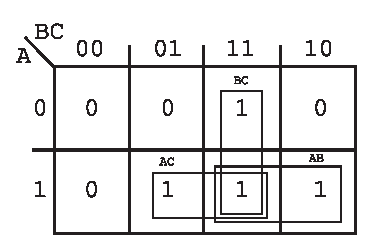
\includegraphics[height=1.25in]{c_bal0/kmap23db.eps}
\caption{Karnaugh Map Of 2/3 Debouncing}
\label{fig:cbal0:svct0:sttd0:01}
\end{figure}

It can be seen from the figure that the expression for the output is

\begin{equation}
\label{eq:cbal0:svct0:sttd0:01}
AB + AC + BC = A (B+C) + BC .
\end{equation}

Intuitively, (\ref{eq:cbal0:svct0:sttd0:01}) makes sense---the output 
will be 1 if any two of the most recent samples are 1
($AB + AC + BC$).  Similarly, the output will be 0 if any two of
the most recent samples are 0.

Figure \ref{fig:cbal0:svct0:sttd0:02} supplies the C-language
code to implement 2/3 debouncing as a vertical mapping.
A C-compiler will typically implement this code very directly
using the bitwise logical instructions of the machine.

\begin{figure}
\begin{verbatim}
/**************************************************************/
/* Assume:                                                    */
/*    A      : Most recent sample (i.e. at t(0)), arranged as */
/*             a group of 8 bits.                             */
/*    B      : Next most recent sample t(-1).                 */
/*    C      : Oldest sample t(-2).                           */
/*    output : Debounced collection of 8 bits presented to    */
/*             software internals.                            */
/**************************************************************/

output = (A & (B | C)) | (B & C);

/* End of code. */
\end{verbatim}
\caption{C-Language Implementation Of 2/3 Debouncing}
\label{fig:cbal0:svct0:sttd0:02}
\end{figure}

\subsection{3/3 Debouncing Vertical Counter}
%Subsection Tag: TTD1.
\label{cbal0:svct0:sttd1}

\index{debouncing}\index{debouncing!3/3}\emph{3/3 debouncing} 
is debouncing where all three of the most recent
three samples must be at a value (either 0 or 1) to cause the 
debounced output to transition to that same value.

Note that 3/3 debouncing as we present it is a sequential (rather than
a purely combinational) mapping from the 3 most recent samples to the
debounced output.  In addition to the 3 inputs, the behavior of the
mapping depends on a single bit of state which is held.  (In the
implementation presented in this section, the state and the debounced
output are the same bit.)  For example, if 2 of the 3 most recent
input samples are 1, the debounced output value may be either 0
or 1.  The transition of the debounced output value from
0 to 1 or from 1 to 0 can only occur if all 3 most recent samples
are 1 or are 0, respectively.

If $A$ is the most recent sample, $B$ is the next-most-recent sample,
$C$ is the oldest sample, and $O$ is the output (assumed maintained
as a RAM location) Fig. \ref{fig:cbal0:svct0:sttd1:01} 
supplies the Karnaugh map for 3/3
debouncing.

\begin{figure}
\centering
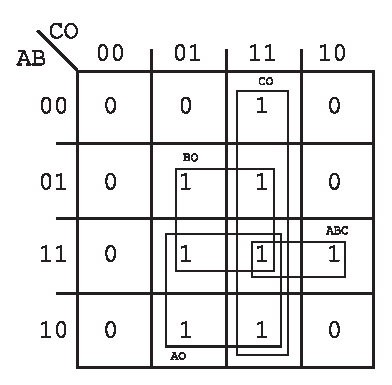
\includegraphics[height=2.0in]{c_bal0/kmap33db.eps}
\caption{Karnaugh Map Of 3/3 Debouncing}
\label{fig:cbal0:svct0:sttd1:01}
\end{figure}

It can be seen from the figure that the expression for the output is

\begin{equation}
\label{eq:cbal0:svct0:sttd1:01}
ABC + AO + BO + CO = ABC + O(A + B + C).
\end{equation}

Intuitively, (\ref{eq:cbal0:svct0:sttd1:01}) makes sense---the output 
will be unconditionally 1 if all three of the most recent samples are 1
($ABC$).  The output will also be 1 if the previous output was 1
and at least one of the most recent samples are 1 [$O(A+B+C)$]---at least
one true recent sample blocks the output from transition to 0.

Figure \ref{fig:cbal0:svct0:sttd1:02} supplies the C-language
code to implement 3/3 debouncing as a vertical mapping.
A C-compiler will typically implement this code very directly
using the bitwise logical instructions of the machine.

\begin{figure}
\begin{verbatim}
/**************************************************************/
/* Assume:                                                    */
/*    A      : Most recent sample (i.e. at t(0)), arranged as */
/*             a group of 8 bits.                             */
/*    B      : Next most recent sample t(-1).                 */
/*    C      : Oldest sample t(-2).                           */
/*    output : Debounced collection of 8 bits presented to    */
/*             software internals.  Note that this is both    */
/*             an input (to the combinational mapping) and    */
/*             the new result.                                */
/**************************************************************/

output = (A & B & C) | (output & (A | B | C));

/* End of code. */
\end{verbatim}
\caption{C-Language Implementation Of 3/3 Debouncing}
\label{fig:cbal0:svct0:sttd1:02}
\end{figure}

\subsection{N/N Debouncing Vertical Counter}
%Subsection Tag: NNC0.
\label{cbal0:svct0:snnc0}

\index{debouncing}\index{debouncing!N/N}It is clear from 
the design of the 3/3 debouncing
vertical counter (Section \ref{cbal0:svct0:sttd1}, immediately
above) that the design of the 3/3 debouncing vertical counter
can be generalized to cover any number of recent samples.
We call such a debouncing vertical counter an N/N debouncing
vertical counter.  In order for the output of such a counter to
turn 1, all $N$ most recent samples must be 1.  Similarly, in order
for such a counter to turn 0, all $N$ most recent samples must be 0.

We rely on a logical argument to design such a N/N debouncing
vertical counter, rather than on Karnaugh maps.  If $I_1 \ldots I_N$
are the $N$ most recent input samples and $O$ is the most recent
output (assumed stored in RAM), it is clear from the form of
(\ref{eq:cbal0:svct0:sttd1:01}) that the formula for the new output
as a function of the inputs $I_1 \ldots I_N$ and the 
most recent output $O_{k-1}$ must be:

\begin{equation}
\label{eq:cbal0:svct0:snnc0:01}
O_k = I_1 I_2 \ldots I_N + (O_{k-1} (I_1 + I_2 + \ldots + I_N)) .
\end{equation}

The form of (\ref{eq:cbal0:svct0:snnc0:01}) is intuitively 
plausible.  If the previous output $O_{k-1}$ is 0, the only
circumstance under which the next output $O_k$ will become 1
is if all $N$ inputs $I_1, I_2, \ldots , I_N$ are 1.
Similarly, if the previous output $O_{k-1}$ is 1, the only
circumstance under which $O_k$ will become 0
is if all $N$ inputs $I_1, I_2, \ldots , I_N$ are 0.  This
is the desired behavior.

For an N/N counter when a large number of previous samples
are required to be at the same value (say, $N=10$, for example),
it may seem that the efficiency of the N/N vertical counter
design presented here will break down.  However, it must be
remembered that the vertical counter approach manipulates
a large number (usually 8 or 16) inputs at a time.  It can be
shown easily that an N/N debouncing vertical counter requires
$2N$ operations to determine the next output.  Thus, for a
10/10 debouncing vertical counter, the necessary software 
may execute in as little as 20 machine instructions.  It would
be difficult to find another method which will perform 10/10
debouncing for 8 or 16 inputs in only 20 machine instructions, thus
we maintain that the N/N debouncing vertical counter
approach presented is quite efficient even for larger
$N$.


\section{Authors And Acknowledgements}
%Section tag:  ACK0
This chapter was primarily written by David T. Ashley
\cite{bibref:i:daveashley}.

We are very grateful to \index{Dattalo, Scott}Scott Dattalo 
\cite{bibref:i:scottdattalo},
whose web pages about vertical counters provided much of the
material for the Section \ref{cbal0:svct0}.
Special thanks to \index{Virgil}Virgil \cite{bibref:i:virgil},
\index{Dresner, Norm}Norm Dresner \cite{bibref:i:normdresner},
and \index{Kaskelma, Heikki}Heikki Kaskelma \cite{bibref:i:heikkikaskelma}
for mathematical assistance provided via the 
\index{sci.math newsgroup@\texttt{sci.math} newsgroup}%
\texttt{sci.math} \cite{bibref:n:scimathnewsgroup} newsgroup.


\section{Exercises}

TBD.

%End of file c_bal0.tex



%Chapter:  Quantization
\chapter{\cquazerolongtitle{}}

\label{cqua0}

\section{Introduction}
%Section tag INT

A microcontroller can inherently manipulate only integers:  usually 8-bit
integers, 16-bit integers, or 32-bit integers.  Typically, the less
expensive a microcontroller is, the smaller the maximum data sizes that
it can accomodate; the least expensive devices can easily manipulate
only integers no larger than 8 bits.

This chapter deals with the error analysis of \emph{quantization}.  By
\emph{quantization}, we mean three [distinct] mechanisms of error introduction
in microcontroller software.

\begin{itemize}
\item \textbf{Input Quantization:} the unavoidable conversion from
      $\vworkrealset$ to $\vworkintset$ performed by interface hardware.
      For example, interface hardware may convert a voltage which is
      conceptually continuous to an integer (which can assume only discrete
      values), or may convert a time period which is conceptually
      continuous to an integer.
\item \textbf{Arithmetic Quantization:} microcontroller arithmetic algorithms
      must often discard precision in order to restrict intermediate results of
      calculations to data sizes which the microcontroller can economically
      manipulate.  This type of quantization error is most often injected
      by discarding the remainder of an integer quotient.
\item \textbf{Output Quantization:} microcontroller output hardware can
      produce continuous outputs (such as voltages or pulse widths)
      only in discrete steps.  Often, this lack of ability to control
      outputs precisely introduces additional uncertainty into the
      system which must be analyzed.
\end{itemize}

Note that the error-injection mechanism that we call \emph{quantization}
(in some sense, the creation of a discrete-\emph{data} system)
is not related to and is orthogonal to the notion of a
discrete-\emph{time} (or sampled) system.


\section{Modeling Of Quantization}
%Section tag: MOQ

For the analytical treatment of quantization, the \emph{floor($\cdot{}$)}
function, denoted $\lfloor \cdot \rfloor$, is used, often preceded by a
scaling factor.  For example, in the case of an A/D converter which
converts a voltage $\in [0, 5]$ volts into an integer
$\in [0,255]_{\vworkintsetnonneg{}}$, we may model the function which
maps from voltage to A/D count as

\begin{equation}
\label{eq:cqua0:smoq:001}
f(x) = \left\lfloor {\frac{255 x }{5}} \right\rfloor .
\end{equation}

Inherent in (\ref{eq:cqua0:smoq:001})
is the assumption that quantization will
choose an integer by rounding \emph{down}.  Other
assumptions are possible
(\ref{eq:cqua0:smoq:002}, \ref{eq:cqua0:smoq:003}).

\begin{equation}
\label{eq:cqua0:smoq:002}
f(x) = \left\lceil {\frac{255 x }{5}} \right\rceil
\end{equation}

\begin{equation}
\label{eq:cqua0:smoq:003}
f(x) = \left\lfloor {\frac{255 x }{5} + \frac{1}{2}} \right\rfloor
\end{equation}

At first glance, it may seem intuitively likely
that (\ref{eq:cqua0:smoq:003}) leads
to smaller error terms than (\ref{eq:cqua0:smoq:001})
or (\ref{eq:cqua0:smoq:002})---that rounding to the
nearest integer is a better strategy than rounding
down or rounding up.  In this case, intuition may be misleading.
(\ref{eq:cqua0:smoq:003}) more precisely \emph{centers the
expected value} of the error than (\ref{eq:cqua0:smoq:001})
or (\ref{eq:cqua0:smoq:002}), but the \emph{span} of the
error---the largest error minus the smallest error---remains
one.  In a practical system, the \emph{span} of the error
is the dominant effect.  In practice,
(\ref{eq:cqua0:smoq:001}), (\ref{eq:cqua0:smoq:002}),
and (\ref{eq:cqua0:smoq:003}) lead to near-identical
error terms.  For algebraic convenience,
(\ref{eq:cqua0:smoq:001}) is used preferentially.

Error terms are denoted by the Greek
letter \emph{epsilon} ($\varepsilon$) and
are viewed as the perturbation to the
``ideal'' to yield the ``actual''; so that a negative error
term leads to a result less than than it
``should'' be, and a positive
error term leads to a result greater than
it ``should'' be.  If the \emph{floor($\cdot{}$)}
is used to model quantization, the relationship
in (\ref{eq:cqua0:smoq:004}) holds.

\begin{equation}
\label{eq:cqua0:smoq:004}
\lfloor x \rfloor = x - \varepsilon{}; \; \varepsilon \in [0,1)
\end{equation}


\section{Error Analysis Of Addition Of Quantized Inputs}
%Section tag: eaqi

If we add two quantized values $\lfloor a \rfloor$ and
$\lfloor b \rfloor$, both $a$ and $b$ contain quantization
error, and a question of interest is how much
error the sum $\lfloor a \rfloor + \lfloor b \rfloor$ may
contain; that is, how different it may be from $a+b$.\footnote{For
addition and subtraction, this question is nearly trivial; but for
multiplication and division the relationships are more complex; and for
an arbitrary network of addition, subtraction, multiplication, and
division we are not sure how to answer this question easily.
Please see \ldots{}.}
We seek an inequality which bounds

\begin{equation}
\label{eq:cqua0:eaqi:001}
\varepsilon{} = \left( {\lfloor a \rfloor + \lfloor b \rfloor} \right)
                      - \left( {a + b} \right)  .
\end{equation}

Noting that quantization introduces an error $\varepsilon \in [0,1)$
(Eq. \ref{eq:cqua0:eaqi:001}) leads to
(\ref{eq:cqua0:eaqi:002}) and (\ref{eq:cqua0:eaqi:003}), which are equivalent statements.

\begin{equation}
\label{eq:cqua0:eaqi:002}
a + b - 2 < \lfloor a \rfloor + \lfloor b \rfloor \leq a + b
\end{equation}

\begin{equation}
\label{eq:cqua0:eaqi:003}
\varepsilon \in (-2,0]
\end{equation}

Extending (\ref{eq:cqua0:eaqi:002}) and (\ref{eq:cqua0:eaqi:003})
to an arbitrary number $N \in \vworkintsetpos{}$ of quantized inputs leads to
(\ref{eq:cqua0:eaqi:004}) and (\ref{eq:cqua0:eaqi:005}),
which are equivalent statements.

\begin{equation}
\label{eq:cqua0:eaqi:004}
\sum_{i=1}^{N} x_i - N < \sum_{i=1}^{N} \lfloor x_i \rfloor \leq \sum_{i=1}^{N} x_i
\end{equation}

\begin{equation}
\label{eq:cqua0:eaqi:005}
\varepsilon \in (-N,0]
\end{equation}

\section{Error Analysis Of Subtraction Of Quantized Inputs}

\section{Error Analysis Of Multiplication Of Quantized Inputs}

\section{Error Analysis Of Division Of Quantized Inputs}

\begin{equation}
\frac{p-1}{q}
<
\frac{\lfloor p \rfloor}{\lfloor q \rfloor}
<
\frac{p}{q-1}; \; p,q > 1
\end{equation}

\section{Error Analysis Of Arbitrary Algebraic Functions}

\section{Error Analysis Of Rational Sweeps}

\section{Exercises}

%End of file c_qua0.tex



%Chapter:  Miscellaneous Topics From Mathematics And Number Theory
%$Header: svn://localhost/dtapublic/pubs/books/ucbka/trunk/c_mtn0/c_mtn0.tex 278 2019-08-14 23:10:36Z dashley $

\chapter[\cmtnzeroshorttitle{}]{\cmtnzerolongtitle{}}

\label{cmtn0}

\beginchapterquote{``If intellectual curiosity, professional pride, and ambition are
                     the dominant incentives to research, then assuredly no one has
                     a fairer chance of gratifying them than a mathematician.  His
                     subject is the most curious of all---there is none in which
                     truth plays such odd pranks.  It has the most elaborate
                     and the most fascinating technique, and gives unrivaled
                     openings for the display of sheer professional skill.  Finally,
                     as history proves abundantly, mathematical achievement, whatever
                     its intrinsic worth, is the most enduring
                     of all.''}
                     {G.H. Hardy \cite{bibref:b:mathematiciansapology:1940}}

\section{Introduction}
%Section Tag: INT0
\label{cmtn0:sint0}


%%%%%%%%%%%%%%%%%%%%%%%%%%%%%%%%%%%%%%%%%%%%%%%%%%%%%%%%%%%%%%%%%%%%%%%%%%%%%%%
%%%%%%%%%%%%%%%%%%%%%%%%%%%%%%%%%%%%%%%%%%%%%%%%%%%%%%%%%%%%%%%%%%%%%%%%%%%%%%%
%%%%%%%%%%%%%%%%%%%%%%%%%%%%%%%%%%%%%%%%%%%%%%%%%%%%%%%%%%%%%%%%%%%%%%%%%%%%%%%

\index{floor function@floor function ($\lfloor\cdot\rfloor$)}%
\index{--@$\lfloor\cdot\rfloor$ (\emph{floor($\cdot$)} function)}%
\index{ceiling function@ceiling function ($\lceil\cdot\rceil$)}%
\index{--@$\lceil\cdot\rceil$ (\emph{ceiling($\cdot$)} function)}%
\section{The Floor \mbox{\boldmath $\lfloor\cdot\rfloor$} And Ceiling \mbox{\boldmath $\lceil\cdot\rceil$} Functions}
\label{cmtn0:sfcf0}

The \emph{floor} function, denoted $\lfloor\cdot\rfloor$, is defined to return
the largest integer not larger than the argument.  For example, 
$\lfloor 3 \rfloor = \lfloor 3.9999 \rfloor = 3$.  For negative arguments, the definition
is identical:  $\lfloor -4 \rfloor = \lfloor -3.9 \rfloor = -4$.

The \emph{ceiling} function, denoted $\lceil\cdot\rceil$, is defined to return
the smallest integer not less than the argument.  For example, 
$\lceil 3.0001 \rceil = \lceil 4 \rceil = 4$.  For negative arguments, the definition
is identical:  $\lceil -4 \rceil = \lceil -4.9 \rceil = -4$.

Note that the definitions presented above for negative arguments
differ from what is commonly implemented in spreadsheet software and other consumer
software.

It can be verfied easily that for 
$a \in \vworkintsetnonneg$, $b \in \vworkintsetpos$,

\begin{equation}
\label{eq:cmtn0:sfcf0:01}
\frac{a}{b} = \left\lfloor\frac{a}{b}\right\rfloor + \frac{a \bmod b}{b}
\end{equation}

\noindent{}and consequently that

\begin{equation}
\label{eq:cmtn0:sfcf0:02}
\left\lfloor\frac{a}{b}\right\rfloor = \frac{a}{b} - \frac{a \bmod b}{b} .
\end{equation}

\noindent{}(\ref{eq:cmtn0:sfcf0:02}) is a very useful identity for 
decomposing expressions involving the \emph{floor($\cdot$)} function.

\section{Tests For Divisibility Of Integers}
%Section Tag: TDI0

%%%%%%%%%%%%%%%%%%%%%%%%%%%%%%%%%%%%%%%%%%%%%%%%%%%%%%%%%%%%%%%%%%%%%%%%%%%%%%%
%%%%%%%%%%%%%%%%%%%%%%%%%%%%%%%%%%%%%%%%%%%%%%%%%%%%%%%%%%%%%%%%%%%%%%%%%%%%%%%
%%%%%%%%%%%%%%%%%%%%%%%%%%%%%%%%%%%%%%%%%%%%%%%%%%%%%%%%%%%%%%%%%%%%%%%%%%%%%%%
\subsection{Tests For Divisibility By 2, 3, 5, 6, 7, And 11}

It is often useful to be able to inspect a radix-10 integer and quickly
determine if it can be divided by a small prime number.  This section
presents tests which can be used to easily determine divisibility by
2, 3, 5, 7, and 11.

Placeholder\index{divisibility tests for integers!by 0002@by 2}
reserved for divisibility by 2.

Placeholder\index{divisibility tests for integers!by 0003@by 3}
reserved for divisibility by 3.

Placeholder\index{divisibility tests for integers!by 0005@by 5}
reserved for divisibility by 5.

Placeholder\index{divisibility tests for integers!by 0007@by 7}
reserved for divisibility by 7.

Placeholder\index{divisibility tests for integers!by 0011@by 11}
reserved for divisibility by 11.


%%%%%%%%%%%%%%%%%%%%%%%%%%%%%%%%%%%%%%%%%%%%%%%%%%%%%%%%%%%%%%%%%%%%%%%%%%%%%%%
%%%%%%%%%%%%%%%%%%%%%%%%%%%%%%%%%%%%%%%%%%%%%%%%%%%%%%%%%%%%%%%%%%%%%%%%%%%%%%%
%%%%%%%%%%%%%%%%%%%%%%%%%%%%%%%%%%%%%%%%%%%%%%%%%%%%%%%%%%%%%%%%%%%%%%%%%%%%%%%
\subsection{Tests For Divisibility By  2$^N$, 6, 9, And 10$^N$}

Placeholder\index{divisibility tests for integers!by 0002N@by 2$^N$}
reserved for divisibility by 2$^N$.

Placeholder\index{divisibility tests for integers!by 0006@by 6}
reserved for divisibility by 6.

Placeholder\index{divisibility tests for integers!by 0009@by 9}
reserved for divisibility by 9.

Placeholder\index{divisibility tests for integers!by 0010N@by 10$^N$}
reserved for divisibility by 10$^N$.


\subsection{David G. Radcliffe's Proof:  Rearrangement Of Digits Of $2^N$}
%Subsection Tag: DGR0

In 07/00, Paul Harvey (\texttt{pharvey@derwent.co.uk}) made the following
post to \texttt{sci.math} \cite{bibref:n:scimathnewsgroup}:

\begin{quote}
{I've got a little problem which is bugging me, perhaps someone out there
can point me in the right direction \ldots{}}

{Does there exist a positive integer which is a power of 2, whose digits can
be rearranged to give a different power of 2?}
\end{quote}

David G. Radcliffe \cite{bibref:i:davidgradcliffe}
responded with a beautiful proof, which is presented below
as a theorem.

\begin{vworktheoremstatement}
No radix-10 positive integral power of 2 (i.e. 1, 2, 4, 8, 16, 32, etc.), with
any leading 0's removed, can be used
to form another radix-10 positive integral power of 2 by simple rearrangement
of the digits.
\end{vworktheoremstatement}
\begin{vworktheoremproof}
Suppose that $x$ and $y$ are two different powers of 2, $y>x$, and that
the digits of $x$ can be rearranged to form $y$.  $y<10x$, since both
$x$ and $y$ must have the same number of digits.  Thus, there
are three possibilities, $y=2x$, $y=4x$, or $y=8x$.

Since $x$ and $y$ have the same digits, but in a different order,
the sum of the digits of $x$ is equal to the sum of the digits of $y$.
It follows that $y-x$ is divisible by 9.  (This follows because
the sum of the digits of an integer $i$, summing the intermediate
sums as many times as necessary to yield a single-digit result,
yield either 9 implying that $i \; mod \; 9 = 0$, or yielding $i \; mod \; 9$.
If the digits of $x$ and $y$ are the same,
the sums of their digits are the same, thus $(x \; mod \; 9) = (y \; mod \; 9)$,
which implies that $((y-x) \; mod \; 9) = 0$, i.e. that $y-x$ is divisible
by 9.)

If $y \in \{ 2x, 4x, 8x \}$, then $y-x \in \{ x, 3x, 7x \}$.  It would
follow that $x$ is divisible by 3, a contradiction.
\end{vworktheoremproof}
\vworktheoremfooter{}

%%%%%%%%%%%%%%%%%%%%%%%%%%%%%%%%%%%%%%%%%%%%%%%%%%%%%%%%%%%%%%%%%%%%%%%%%%%%%%%
%%%%%%%%%%%%%%%%%%%%%%%%%%%%%%%%%%%%%%%%%%%%%%%%%%%%%%%%%%%%%%%%%%%%%%%%%%%%%%%
%%%%%%%%%%%%%%%%%%%%%%%%%%%%%%%%%%%%%%%%%%%%%%%%%%%%%%%%%%%%%%%%%%%%%%%%%%%%%%%
\section{The Pigeonhole Principle}
\label{cmtn0:sphp0}

The \index{pigeonhole principle}\emph{pigeonhole principle} is a statement 
that if $m$ items are placed into $n$ slots, with $m > n$, then at least one
slot will contain more than one item.  This is also known as
\index{Dirichlet's box principle}\emph{Dirichlet's box principle}.

A related statement is that $m$ items are placed into $n$ slots, 
with $m < n$, then at least one
slot will be empty.

Despite its simplicity, the pigeonhole principle is the basis for many important
proofs and observations in number theory.


%%%%%%%%%%%%%%%%%%%%%%%%%%%%%%%%%%%%%%%%%%%%%%%%%%%%%%%%%%%%%%%%%%%%%%%%%%%%%%%
%%%%%%%%%%%%%%%%%%%%%%%%%%%%%%%%%%%%%%%%%%%%%%%%%%%%%%%%%%%%%%%%%%%%%%%%%%%%%%%
%%%%%%%%%%%%%%%%%%%%%%%%%%%%%%%%%%%%%%%%%%%%%%%%%%%%%%%%%%%%%%%%%%%%%%%%%%%%%%%
\section{Exercises}


%%%%%%%%%%%%%%%%%%%%%%%%%%%%%%%%%%%%%%%%%%%%%%%%%%%%%%%%%%%%%%%%%%%%%%%%%%%%%%%

\noindent\begin{figure}[!b]
\noindent\rule[-0.25in]{\textwidth}{1pt}
\begin{tiny}
\begin{verbatim}
$HeadURL: svn://localhost/dtapublic/pubs/books/ucbka/trunk/c_mtn0/c_mtn0.tex $
$Revision: 278 $
$Date: 2019-08-14 19:10:36 -0400 (Wed, 14 Aug 2019) $
$Author: dashley $
\end{verbatim}
\end{tiny}
\noindent\rule[0.25in]{\textwidth}{1pt}
\end{figure}

%%%%%%%%%%%%%%%%%%%%%%%%%%%%%%%%%%%%%%%%%%%%%%%%%%%%%%%%%%%%%%%%%%%%%%%%%%%%%%%
%
%End of file C_MTN0.TEX


% New part: Construction Of Embedded Software
\part{Construction Of Embedded Software}

%Chapter:  General Practical Construction Of Embedded Software
%$Header: svn://localhost/dtapublic/pubs/books/ucbka/trunk/c_pco0/c_pco0.tex 278 2019-08-14 23:10:36Z dashley $

\chapter{\cpcozerolongtitle{}}

\label{cpco0}

\beginchapterquote{``For any serious purpose, intelligence is a very minor gift.''}
                     {G. H. Hardy, \cite{bibref:b:mathematiciansapology:1940}}

%%%%%%%%%%%%%%%%%%%%%%%%%%%%%%%%%%%%%%%%%%%%%%%%%%%%%%%%%%%%%%%%%%%%%%%%%%
%%%%%%%%%%%%%%%%%%%%%%%%%%%%%%%%%%%%%%%%%%%%%%%%%%%%%%%%%%%%%%%%%%%%%%%%%%
%%%%%%%%%%%%%%%%%%%%%%%%%%%%%%%%%%%%%%%%%%%%%%%%%%%%%%%%%%%%%%%%%%%%%%%%%%
\section{Introduction}
%Section tag: INT0
\label{cpco0:sint0}

In this chapter, we explain in detail the way that
practical microcontroller software is constructed.
Such discussion is essential for two reasons:

\begin{itemize}
\item Practical techniques of construction, because they have 
      been honed over time, usually represent best practices.
      The techniques presented in this chapter represent worthy
      techniques for constructing embedded systems, and may
      serve as a guide for the construction of embedded software.
\item Software engineers often grasp concepts intuitively that they
      cannot express formally.  Many of the tendencies and best practices
      described in this chapter have a formal basis that can and should be
      studied and investigated.
\end{itemize}


%%%%%%%%%%%%%%%%%%%%%%%%%%%%%%%%%%%%%%%%%%%%%%%%%%%%%%%%%%%%%%%%%%%%%%%%%%
%%%%%%%%%%%%%%%%%%%%%%%%%%%%%%%%%%%%%%%%%%%%%%%%%%%%%%%%%%%%%%%%%%%%%%%%%%
%%%%%%%%%%%%%%%%%%%%%%%%%%%%%%%%%%%%%%%%%%%%%%%%%%%%%%%%%%%%%%%%%%%%%%%%%%
\section{Measurement Of Time}
%Section tag: MOT0
\label{cpco0:smot0}

As we've mentioned previously, most software components in a
typical small embedded system are state machines with transition
functions that depend on inputs and on time.

Because time is such a perasive concept in microcontroller software,
the decision about how time is to be measured and tested is the
single most important design decision in terms of ROM consumption.


%%%%%%%%%%%%%%%%%%%%%%%%%%%%%%%%%%%%%%%%%%%%%%%%%%%%%%%%%%%%%%%%%%%%%%%%%%
%%%%%%%%%%%%%%%%%%%%%%%%%%%%%%%%%%%%%%%%%%%%%%%%%%%%%%%%%%%%%%%%%%%%%%%%%%
%%%%%%%%%%%%%%%%%%%%%%%%%%%%%%%%%%%%%%%%%%%%%%%%%%%%%%%%%%%%%%%%%%%%%%%%%%
\subsection{Countdown Software Timers}
%Subsection tag: CST0
\label{cpco0:smot0:scst0}

The most common mechanism for allowing state machines to make transitions
which are partly based on time is the 
\index{countdown software timer}\emph{countdown software timer},
which is most commonly called a 
\index{software timer}\emph{software timer}.

A software timer is an unsigned byte or word which is decremented at a 
periodic rate, but never decremented beyond zero.  All software 
timers in a system are typically decremented by one system process.
A process which uses a software timer will set (assign) it to
a non-zero value representing a time delay, and then test it against 
zero to check if the time delay has elapsed.  This approach has
several advantages:

\begin{itemize}
\item Setting a software timer (assigning it to a non-zero
      value) is a very inexpensive and compact test.  (Because
      the setting of software timers occurs many times throughout
      ROM, this savings can be substantial.  Additionally,
      there is a savings in execution time.)
\item A test of a byte against zero is typically a very 
      inexpensive and compact test.  (Because tests for
      expired timers occur many times throughout ROM,
      this savings can be substantial.  Additionally, there
      is a large savings in execution time because 
      in a typical software load, \emph{many} transition
      functions depend on expired timers.)
\item Decrements of single bytes, as are required
      to decrement software timers, are also inexpensive operations.
\end{itemize}

Because software timers are either one unsigned byte (8 bits) or
one unsigned word (16 bits), it is not possible to have ``one size
fits all'', as the range of a software timer and its precision
are mutually exclusive.  Very typically, software timers are arranged 
in either binary decades (for example, 2 ms/count, 4 ms/count, 
8 ms/count, 16 ms/count, etc.) or in the more conventional
1-2-5 decades (for example, 1 ms/count, 2 ms/count, 5 ms/count,
10 ms/count, etc.).

Because the process which uses a software timer as a time 
reference and the process which decrements a software timer
are asynchronous, a process which sets a software timer has no 
control over whether the timer will be decremented for the
first time immediately or after the period-per-count of the timer.
Generally, if $\tau$ is the period-per-count of a software timer and
the software timer is set to the value of $N$, the process that
sets the software timer can be assured that the time $T$ until the
software timer reaches zero will meet the inequality

\begin{equation}
\label{eq:cpco0:smot0:scst0:00}
(N-1) \tau < T \leq N \tau ,
\end{equation}

\noindent{}where the interval is open on the left because 
it is not possible to test a software timer at
the same instant it is set.

Despite the inequality supplied by 
(\ref{eq:cpco0:smot0:scst0:00}), it is common in practice to calculate
the value to which a software timer should be set as

\begin{equation}
\label{eq:cpco0:smot0:scst0:01}
N = \left\lfloor { \frac{T}{\tau} } \right\rfloor .
\end{equation}

(\ref{eq:cpco0:smot0:scst0:01}) is commonly used because there
are other sources of delay in a software system that compensate
for the lower bound in (\ref{eq:cpco0:smot0:scst0:00}), and because
values of $N$ are seldom close to zero, so any error due to the
lower bound is small in relation to $T$.

It is also instructive to calculate the maximum ``coarseness'' when 
software timers are arranged in binary decades or 1-2-5 decades
and consequently a period-per-count $\tau$ which precisely accomodates
the maximum period $T$ cannot be chosen.  In the case of binary decades,
the inequality

\begin{equation}
\label{eq:cpco0:smot0:scst0:02}
\frac{255}{2} \tau < T \leq 255 \tau
\end{equation}

\noindent{}holds, as if it were true that $T \leq 255 \tau /2$, 
then we would choose
a software timer with the next smaller period $\tau ' = \tau / 2$.
Thus we are always assured that

\begin{equation}
\label{eq:cpco0:smot0:scst0:03}
\tau < 127.5 T .
\end{equation}

\noindent{}Thus, with a binary decade arrangement of software timers, we
can always choose the timer period $N \tau$ with a granularity of about
1 part in 127.5 or better.

The analogous question for software timers arranged in 1-2-5 decades
leads to this inequality:

\begin{equation}
\label{eq:cpco0:smot0:scst0:04}
\frac{255}{2.5} \tau < T \leq 255 \tau ,
\end{equation}

\noindent{}where the factor ``2.5'' appears because the largest
change in $\tau$ will occur from ``2'' to ``5'' in a 1-2-5 decade
arrangement.  Again, the same argument made earlier 
applies---if $T \leq 255 \tau / 2.5$, then it would \emph{always}
be possible to choose a software timer with the next smaller period.
Thus we are always assured that

\begin{equation}
\label{eq:cpco0:smot0:scst0:05}
\tau < 102 T .
\end{equation}

\noindent{}Thus, with a 1-2-5 decade arrangement of software timers, we
can always choose the timer period $N \tau$ with a granularity of about
1 part in 102 or better.


%%%%%%%%%%%%%%%%%%%%%%%%%%%%%%%%%%%%%%%%%%%%%%%%%%%%%%%%%%%%%%%%%%%%%%%%%%
%%%%%%%%%%%%%%%%%%%%%%%%%%%%%%%%%%%%%%%%%%%%%%%%%%%%%%%%%%%%%%%%%%%%%%%%%%
%%%%%%%%%%%%%%%%%%%%%%%%%%%%%%%%%%%%%%%%%%%%%%%%%%%%%%%%%%%%%%%%%%%%%%%%%%
\subsection{On-Demand Two's Complement Timekeeping}
%Subsection tag: ODT0
\label{cpco0:smot0:sodt0}

Often, software timers as described in Section \ref{cpco0:smot0:scst0}
immediately above won't meet a particular timing requirement because
the period to be measured is quite large, but it must be measured with
fair precision.\footnote{A typical requirement with these characteristics
is that a delay be 60 minutes $\pm$ 5 seconds.  This requirement
represents a precision of 1 part in 720, which is more precision
than a 1-byte software timer can offer.}  

In such situations, one 
option is to offer extended-precision (i.e. 16- or 24-bit) software timers.
However, another popular option is to provide a function call which
will allow retrieval of the most precise time measurement available,
typically maintained as a multiple-precision integer.  A typical
design decision in microcontroller work would be a 5-byte multiple-precision
integer counter, maintaining the number of milliseconds since the 
microcontroller was reset.  Such a counter will measure time periods
of up to about 35 years.

Note that in using the value obtained from a function call
which obtains a maximum-precision time count, it is not
necessary to use all the bytes of the result.  For example,
using the least significant two bytes of such a counter
(assuming that the counter represents milliseconds) will
allow the measurement of time periods up to about 65 seconds
with 1ms of resolution.


%%%%%%%%%%%%%%%%%%%%%%%%%%%%%%%%%%%%%%%%%%%%%%%%%%%%%%%%%%%%%%%%%%%%%%%%%%
%%%%%%%%%%%%%%%%%%%%%%%%%%%%%%%%%%%%%%%%%%%%%%%%%%%%%%%%%%%%%%%%%%%%%%%%%%
%%%%%%%%%%%%%%%%%%%%%%%%%%%%%%%%%%%%%%%%%%%%%%%%%%%%%%%%%%%%%%%%%%%%%%%%%%
\subsection{Invocation Counting}
%Subsection tag: ICN0
\label{cpco0:smot0:sicn0}



%%%%%%%%%%%%%%%%%%%%%%%%%%%%%%%%%%%%%%%%%%%%%%%%%%%%%%%%%%%%%%%%%%%%%%%%%%
%%%%%%%%%%%%%%%%%%%%%%%%%%%%%%%%%%%%%%%%%%%%%%%%%%%%%%%%%%%%%%%%%%%%%%%%%%
%%%%%%%%%%%%%%%%%%%%%%%%%%%%%%%%%%%%%%%%%%%%%%%%%%%%%%%%%%%%%%%%%%%%%%%%%%
\subsection{Timer Events}
%Subsection tag: TEV0
\label{cpco0:smot0:stev0}



%%%%%%%%%%%%%%%%%%%%%%%%%%%%%%%%%%%%%%%%%%%%%%%%%%%%%%%%%%%%%%%%%%%%%%%%%%
%%%%%%%%%%%%%%%%%%%%%%%%%%%%%%%%%%%%%%%%%%%%%%%%%%%%%%%%%%%%%%%%%%%%%%%%%%
%%%%%%%%%%%%%%%%%%%%%%%%%%%%%%%%%%%%%%%%%%%%%%%%%%%%%%%%%%%%%%%%%%%%%%%%%%
\section{Interface Styles}
%Section tag: IST0
\label{cpco0:sist0}

Without exception, the paradigm of decomposition for small microcontroller
software is a collection of concurrent cooperating state machines.  In other
words, we imagine
the software system as collection of state machines\footnote{\ldots{} or processes or 
timed automatons or elementary hybrid machines or state machine thingies
or thingamabobs or whatever it is in your lingo, man \ldots{}.} which are
\emph{independent} or \emph{concurrent}:  that is, they can in most 
cases change state independently
of one another.  However, at the same time, we envision these
state machines as \emph{cooperating}:  that is, they have ways 
of exchanging information and of synchronizing when necessary.

In this section, we enumerate and discuss all of the interface
types between 
concurrent cooperating state machines.


%%%%%%%%%%%%%%%%%%%%%%%%%%%%%%%%%%%%%%%%%%%%%%%%%%%%%%%%%%%%%%%%%%%%%%%%%%
%%%%%%%%%%%%%%%%%%%%%%%%%%%%%%%%%%%%%%%%%%%%%%%%%%%%%%%%%%%%%%%%%%%%%%%%%%
%%%%%%%%%%%%%%%%%%%%%%%%%%%%%%%%%%%%%%%%%%%%%%%%%%%%%%%%%%%%%%%%%%%%%%%%%%
\subsection[1-Writer $n$-Reader RAM Variable Interface]
           {1-Writer \mbox{\boldmath $n$}-Reader RAM Variable Interface}
%Subsection tag: own0
\label{cpco0:sist0:sown0}


%%%%%%%%%%%%%%%%%%%%%%%%%%%%%%%%%%%%%%%%%%%%%%%%%%%%%%%%%%%%%%%%%%%%%%%%%%
%%%%%%%%%%%%%%%%%%%%%%%%%%%%%%%%%%%%%%%%%%%%%%%%%%%%%%%%%%%%%%%%%%%%%%%%%%
%%%%%%%%%%%%%%%%%%%%%%%%%%%%%%%%%%%%%%%%%%%%%%%%%%%%%%%%%%%%%%%%%%%%%%%%%%
\subsection{Finite State Machine RAM Variable Interface}
%Subsection tag: fsm0
\label{cpco0:sist0:sfsm0}


%%%%%%%%%%%%%%%%%%%%%%%%%%%%%%%%%%%%%%%%%%%%%%%%%%%%%%%%%%%%%%%%%%%%%%%%%%
%%%%%%%%%%%%%%%%%%%%%%%%%%%%%%%%%%%%%%%%%%%%%%%%%%%%%%%%%%%%%%%%%%%%%%%%%%
%%%%%%%%%%%%%%%%%%%%%%%%%%%%%%%%%%%%%%%%%%%%%%%%%%%%%%%%%%%%%%%%%%%%%%%%%%
\subsubsection{The General FSM RAM Variable Interface}
%Subsubsection tag: gfs0
\label{cpco0:sist0:sfsm0:sgfs0}


%%%%%%%%%%%%%%%%%%%%%%%%%%%%%%%%%%%%%%%%%%%%%%%%%%%%%%%%%%%%%%%%%%%%%%%%%%
%%%%%%%%%%%%%%%%%%%%%%%%%%%%%%%%%%%%%%%%%%%%%%%%%%%%%%%%%%%%%%%%%%%%%%%%%%
%%%%%%%%%%%%%%%%%%%%%%%%%%%%%%%%%%%%%%%%%%%%%%%%%%%%%%%%%%%%%%%%%%%%%%%%%%
\subsubsection{The RAM Variable Semaphore}
%Subsubsection tag: rvs0
\label{cpco0:sist0:sfsm0:srvs0}


%%%%%%%%%%%%%%%%%%%%%%%%%%%%%%%%%%%%%%%%%%%%%%%%%%%%%%%%%%%%%%%%%%%%%%%%%%
%%%%%%%%%%%%%%%%%%%%%%%%%%%%%%%%%%%%%%%%%%%%%%%%%%%%%%%%%%%%%%%%%%%%%%%%%%
%%%%%%%%%%%%%%%%%%%%%%%%%%%%%%%%%%%%%%%%%%%%%%%%%%%%%%%%%%%%%%%%%%%%%%%%%%
\section{Reduction Of Combinational Mappings}



%%%%%%%%%%%%%%%%%%%%%%%%%%%%%%%%%%%%%%%%%%%%%%%%%%%%%%%%%%%%%%%%%%%%%%%%%%
%%%%%%%%%%%%%%%%%%%%%%%%%%%%%%%%%%%%%%%%%%%%%%%%%%%%%%%%%%%%%%%%%%%%%%%%%%
%%%%%%%%%%%%%%%%%%%%%%%%%%%%%%%%%%%%%%%%%%%%%%%%%%%%%%%%%%%%%%%%%%%%%%%%%%
\section{Reduction Of Sequential Mappings}



%%%%%%%%%%%%%%%%%%%%%%%%%%%%%%%%%%%%%%%%%%%%%%%%%%%%%%%%%%%%%%%%%%%%%%%%%%
%%%%%%%%%%%%%%%%%%%%%%%%%%%%%%%%%%%%%%%%%%%%%%%%%%%%%%%%%%%%%%%%%%%%%%%%%%
%%%%%%%%%%%%%%%%%%%%%%%%%%%%%%%%%%%%%%%%%%%%%%%%%%%%%%%%%%%%%%%%%%%%%%%%%%
\section{Debouncing}



%%%%%%%%%%%%%%%%%%%%%%%%%%%%%%%%%%%%%%%%%%%%%%%%%%%%%%%%%%%%%%%%%%%%%%%%%%
%%%%%%%%%%%%%%%%%%%%%%%%%%%%%%%%%%%%%%%%%%%%%%%%%%%%%%%%%%%%%%%%%%%%%%%%%%
%%%%%%%%%%%%%%%%%%%%%%%%%%%%%%%%%%%%%%%%%%%%%%%%%%%%%%%%%%%%%%%%%%%%%%%%%%
\section{Filtering}



%%%%%%%%%%%%%%%%%%%%%%%%%%%%%%%%%%%%%%%%%%%%%%%%%%%%%%%%%%%%%%%%%%%%%%%%%%
%%%%%%%%%%%%%%%%%%%%%%%%%%%%%%%%%%%%%%%%%%%%%%%%%%%%%%%%%%%%%%%%%%%%%%%%%%
%%%%%%%%%%%%%%%%%%%%%%%%%%%%%%%%%%%%%%%%%%%%%%%%%%%%%%%%%%%%%%%%%%%%%%%%%%
\section{ROM Reduction Techniques}
%Section tag: rrs0
\label{cpco0:srrs0}

Microcontroller products are very sensitive to ROM consumption, and
a primary goal is to create a software load that meets all requirements
with minimal ROM.  Semiconductor manufacturers often design 
microcontroller families so that there is a continuum of microcontroller
variants which differ only in the amount of ROM and RAM available,
and in some cases a microcontroller software developer is able to 
substitute a different part with more ROM if a ROM boundary is reached.
However, semiconductor manufacturers always create a pricing schema
where the part with more ROM costs more, and so even if a part with
more ROM is available, there may be substantial management pressure to
shoehorn a software load into the smaller part rather than use the
more expensive part. In many cases, no substitute part with more ROM
is available, so the software load \emph{must} fit.

In this section, we discuss strategies for reducing ROM consumption
in an embedded software load.  For the most part, these are strategies
that can be adopted retroactively when a software load does not fit.
However, it should also be noted that ROM efficiency \emph{starts}
with using some of the construction techniques presented in this chapter
in order to create a ROM-efficient system from the start.  For example, 
an inefficient design decision regarding the measurement of time
would be hard to recover from.


%%%%%%%%%%%%%%%%%%%%%%%%%%%%%%%%%%%%%%%%%%%%%%%%%%%%%%%%%%%%%%%%%%%%%%%%%%
%%%%%%%%%%%%%%%%%%%%%%%%%%%%%%%%%%%%%%%%%%%%%%%%%%%%%%%%%%%%%%%%%%%%%%%%%%
%%%%%%%%%%%%%%%%%%%%%%%%%%%%%%%%%%%%%%%%%%%%%%%%%%%%%%%%%%%%%%%%%%%%%%%%%%
\subsection{Modifying The Largest Software Component First}
%Subsection tag: mlf0
\label{cpco0:srrs0:smlf0}

One observation which is helpful is that the largest software components
in a system tend to have the most absolute ROM waste.\footnote{Thanks
to Lou Miller \cite{bibref:i:loumiller} for this insight.}  
Therefore, the quickest way to significantly reduce the ROM consumption
of an embedded software load is often to analyze and optimize the 
largest software component.


%%%%%%%%%%%%%%%%%%%%%%%%%%%%%%%%%%%%%%%%%%%%%%%%%%%%%%%%%%%%%%%%%%%%%%%%%%
%%%%%%%%%%%%%%%%%%%%%%%%%%%%%%%%%%%%%%%%%%%%%%%%%%%%%%%%%%%%%%%%%%%%%%%%%%
%%%%%%%%%%%%%%%%%%%%%%%%%%%%%%%%%%%%%%%%%%%%%%%%%%%%%%%%%%%%%%%%%%%%%%%%%%
\subsection{Optimizing \emph{near} Versus \emph{far} Allocation Of RAM}
%Subsection tag: nvf0
\label{cpco0:srrs0:snvf0}

Many microcontrollers have two different categories of RAM, which are
usually called \emph{near} and \emph{far} RAM; although some microcontrollers
use different nomenclature---for example \emph{zero page} RAM rather than
\emph{near} RAM.  Usually, \emph{near} and \emph{far} are also 
the `C' keywords used.

Usually, \emph{near} RAM has three advantages over \emph{far} RAM:

\begin{itemize}
\item Machine instructions to access (load, store, test, perform
      arithmetic on) near RAM locations are more compact than the
      corresponding instructions on far RAM.  This normally comes
      directly from the machine-language encoding of instructions:
      most typically the address of a near location requires one byte
      to encode while the address of a far location requires two.
\item Machine instructions to access (load, store, test, perform
      arithmetic on) near RAM locations require less time to
      execute than the
      corresponding instructions on far RAM.  This is normally
      strongly related to the more compact encoding, as there
      are fewer ROM fetches involved.
\item In many cases, certain instructions can operate only on near
      operands.  This means that certain operations applied to
      near operands require only one machine instruction,
      but require at least three (load, operate, store) when 
      applied to far operands.
\end{itemize}

It is intuitively clear that to minimize ROM consumption, assuming that
we have a limited amount of near RAM and cannot place all variables
in near RAM, we must place the most frequently-accessed (throughout
all of ROM) variables in near RAM.

In practice, the allocation of most frequently accessed variables to 
near RAM happens both formally and informally in microcontroller 
software developments.  

Informally, it occurs because it is known
from experience that certain RAM variables are frequently accessed
and should be placed in near RAM---for example, in most automobile
modules, ignition switch position is referenced many times throughout
ROM and software developers know from experience that this is best placed
in near RAM. 

Formally, software developers often produce home-made tools to analyze
the number of times throughout ROM that each variable is referenced, and then
use this information to allocate variables into near and far RAM.
Unfortunately, this process is usually manual and cumbersome.
To the best of our knowledge, as of 9/2001, no compiler will analyze
variable reference information and allocate variables automatically.
(The best way to accompish this would probably to introduce an
addtional keyword that advises the development tools to analyze
the number of references and automatically choose whether a variable should be 
near or far.  \texttt{autonearfar} strikes us as a suitably
suggestive keyword.)


%%%%%%%%%%%%%%%%%%%%%%%%%%%%%%%%%%%%%%%%%%%%%%%%%%%%%%%%%%%%%%%%%%%%%%%%%%
%%%%%%%%%%%%%%%%%%%%%%%%%%%%%%%%%%%%%%%%%%%%%%%%%%%%%%%%%%%%%%%%%%%%%%%%%%
%%%%%%%%%%%%%%%%%%%%%%%%%%%%%%%%%%%%%%%%%%%%%%%%%%%%%%%%%%%%%%%%%%%%%%%%%%
\subsection{Storage Of Intermediate Results In Near RAM}
%Subsection tag: sir0
\label{cpco0:srrs0:ssir0}


%%%%%%%%%%%%%%%%%%%%%%%%%%%%%%%%%%%%%%%%%%%%%%%%%%%%%%%%%%%%%%%%%%%%%%%%%%
%%%%%%%%%%%%%%%%%%%%%%%%%%%%%%%%%%%%%%%%%%%%%%%%%%%%%%%%%%%%%%%%%%%%%%%%%%
%%%%%%%%%%%%%%%%%%%%%%%%%%%%%%%%%%%%%%%%%%%%%%%%%%%%%%%%%%%%%%%%%%%%%%%%%%
\subsection{Suppression Of \emph{Else} Clauses}
%Subsection tag: sec0
\label{cpco0:srrs0:ssec0}


%%%%%%%%%%%%%%%%%%%%%%%%%%%%%%%%%%%%%%%%%%%%%%%%%%%%%%%%%%%%%%%%%%%%%%%%%%
%%%%%%%%%%%%%%%%%%%%%%%%%%%%%%%%%%%%%%%%%%%%%%%%%%%%%%%%%%%%%%%%%%%%%%%%%%
%%%%%%%%%%%%%%%%%%%%%%%%%%%%%%%%%%%%%%%%%%%%%%%%%%%%%%%%%%%%%%%%%%%%%%%%%%
\subsection{Reassignment Of State Variable State Values}
%Subsection tag: rsv0
\label{cpco0:srrs0:srsv0}

Generally, a state machine constains both a discrete state and a
``continuous'' state (software timers).  (In the strictest sense,
the software timers are not discrete state, but they are typically
modeled this way.)  It can be advantageous to give careful thought
to how the numerical values of discrete states are assigned.

The following observations can be made about the influence of the
numerical values of discrete states on ROM consumption:

\begin{itemize}
\item Tests against zero may sometimes be cheaper than
      tests against any other value (depending on the processor
      instruction set).  This may imply that the numerical value
      of zero should be assigned to the state which is most
      often tested for.
\item In some cases, assignment to zero may be cheaper than
      assignment to any other value (i.e. a ``clear" instruction
      versus a ``set'' instruction, depending on the instruction
      set).  This may imply that 
      the numerical value of zero should be assigned to the
      state with the most incoming transitions.
\item It may frequently occur that tests for which discrete
      state the system is in are seeking to detect
      not a single state, but rather a group of states (i.e.
      \texttt{if ((state == STATE\_1) || (state == STATE\_2) || \ldots{} )}).
      In such cases, it may be advantageous to assign numerical values
      to make such tests more economical, i.e. it may be advantageous
      to ``equivalence class'' states (we discuss this in subsequent
      paragraphs).
\end{itemize}

We should add more about the equivalence classing of states.  In this
context, we mean equivalence classing under the instruction set of the
microcontroller.  That is, we seek to find some way to assign numerical
values to states so that some instruction (\emph{any} instruction!) will
break them into the classes we desire.  It is also noteworthy that we seek
as much flexibility (as many options) as possible, because we may wish to
create more than two equivalence classes, and we may also
wish for some states to appear in more than one equivalence class.

Examples of methods to equivalence class are:

\begin{itemize}
\item Using a bitwise ``AND'' instruction to mask out all
      but $n$ bits (of an $N$-bit state variable)
      and test the result
      against zero.  This creates two equivalence
      classes, one of cardinality $2^{N-n}$ 
      and the other of cardinality 
      $2^N - 2^{N-n} = (2^n - 1)(2^{N-n})$.
\item Testing (comparing) against a specific value.  This creates
      equivalence classes of arbitrary cardinality.
\end{itemize}




%%%%%%%%%%%%%%%%%%%%%%%%%%%%%%%%%%%%%%%%%%%%%%%%%%%%%%%%%%%%%%%%%%%%%%%%%%
%%%%%%%%%%%%%%%%%%%%%%%%%%%%%%%%%%%%%%%%%%%%%%%%%%%%%%%%%%%%%%%%%%%%%%%%%%
%%%%%%%%%%%%%%%%%%%%%%%%%%%%%%%%%%%%%%%%%%%%%%%%%%%%%%%%%%%%%%%%%%%%%%%%%%
\subsection{Factoring Of \emph{Any} Repeated Operation}
%Subsection tag: far0
\label{cpco0:srrs0:sfar0}

In a typical microcontroller, a subroutine call requires three bytes in ROM
(one byte for the opcode, and two for the address).  Thus, for any
repeated operation which requires over three bytes to accomplish,
it normally is most effective to place the operation in a subroutine.
Such a technique will exact a performance penalty in exchange for
ROM savings.

Most commonly, such a technique is applied to variable assignments which
accompany state transitions.  However, it can also be applied
to subexpressions in state transition functions.


%%%%%%%%%%%%%%%%%%%%%%%%%%%%%%%%%%%%%%%%%%%%%%%%%%%%%%%%%%%%%%%%%%%%%%%%%%
%%%%%%%%%%%%%%%%%%%%%%%%%%%%%%%%%%%%%%%%%%%%%%%%%%%%%%%%%%%%%%%%%%%%%%%%%%
%%%%%%%%%%%%%%%%%%%%%%%%%%%%%%%%%%%%%%%%%%%%%%%%%%%%%%%%%%%%%%%%%%%%%%%%%%
\subsection{Factoring Of State Transition Functions And Transitions}
%Subsection tag: fst0
\label{cpco0:srrs0:sfst0}



%%%%%%%%%%%%%%%%%%%%%%%%%%%%%%%%%%%%%%%%%%%%%%%%%%%%%%%%%%%%%%%%%%%%%%%%%%
%%%%%%%%%%%%%%%%%%%%%%%%%%%%%%%%%%%%%%%%%%%%%%%%%%%%%%%%%%%%%%%%%%%%%%%%%%
%%%%%%%%%%%%%%%%%%%%%%%%%%%%%%%%%%%%%%%%%%%%%%%%%%%%%%%%%%%%%%%%%%%%%%%%%%
\section{Initialization}



%%%%%%%%%%%%%%%%%%%%%%%%%%%%%%%%%%%%%%%%%%%%%%%%%%%%%%%%%%%%%%%%%%%%%%%%%%
%%%%%%%%%%%%%%%%%%%%%%%%%%%%%%%%%%%%%%%%%%%%%%%%%%%%%%%%%%%%%%%%%%%%%%%%%%
%%%%%%%%%%%%%%%%%%%%%%%%%%%%%%%%%%%%%%%%%%%%%%%%%%%%%%%%%%%%%%%%%%%%%%%%%%
\section{The Interrupt Subsystem}



%%%%%%%%%%%%%%%%%%%%%%%%%%%%%%%%%%%%%%%%%%%%%%%%%%%%%%%%%%%%%%%%%%%%%%%%%%
%%%%%%%%%%%%%%%%%%%%%%%%%%%%%%%%%%%%%%%%%%%%%%%%%%%%%%%%%%%%%%%%%%%%%%%%%%
%%%%%%%%%%%%%%%%%%%%%%%%%%%%%%%%%%%%%%%%%%%%%%%%%%%%%%%%%%%%%%%%%%%%%%%%%%
\section{Sleep And Wakeup}



%%%%%%%%%%%%%%%%%%%%%%%%%%%%%%%%%%%%%%%%%%%%%%%%%%%%%%%%%%%%%%%%%%%%%%%%%%
%%%%%%%%%%%%%%%%%%%%%%%%%%%%%%%%%%%%%%%%%%%%%%%%%%%%%%%%%%%%%%%%%%%%%%%%%%
%%%%%%%%%%%%%%%%%%%%%%%%%%%%%%%%%%%%%%%%%%%%%%%%%%%%%%%%%%%%%%%%%%%%%%%%%%
\vfill
\noindent\begin{figure}[!b]
\noindent\rule[-0.25in]{\textwidth}{1pt}
\begin{tiny}
\begin{verbatim}
$HeadURL: svn://localhost/dtapublic/pubs/books/ucbka/trunk/c_pco0/c_pco0.tex $
$Revision: 278 $
$Date: 2019-08-14 19:10:36 -0400 (Wed, 14 Aug 2019) $
$Author: dashley $
\end{verbatim}
\end{tiny}
\noindent\rule[0.25in]{\textwidth}{1pt}
\end{figure}

%%%%%%%%%%%%%%%%%%%%%%%%%%%%%%%%%%%%%%%%%%%%%%%%%%%%%%%%%%%%%%%%%%%%%%%%%%
%
%End of file C_PCO0.TEX


%Chapter:  Support Of On-Chip Peripherals And Subsystems
\chapter{\csoczerolongtitle{}}

\label{csoc0}

\beginchapterquote{``Under construction!''}
                     {Under construction!}

\section{Introduction}
%Section tag: INT0


\section{Hardware Watchdogs}


\section{EEPROM}

%End of file c_soc0.tex



%Chapter:  Support Of Off-Chip Peripherals And Subsystems
%$Header: svn://localhost/dtapublic/pubs/books/ucbka/trunk/c_soc1/c_soc1.tex 279 2019-08-17 03:10:13Z dashley $

\chapter[\csoconeshorttitle{}]{\csoconelongtitle{}}

\label{csoc1}

\beginchapterquote{``Anything is possible if you don't know what you're talking
                     about.''}
                     {Unknown}

%%%%%%%%%%%%%%%%%%%%%%%%%%%%%%%%%%%%%%%%%%%%%%%%%%%%%%%%%%%%%%%%%%%%%%%%%%
%%%%%%%%%%%%%%%%%%%%%%%%%%%%%%%%%%%%%%%%%%%%%%%%%%%%%%%%%%%%%%%%%%%%%%%%%%
%%%%%%%%%%%%%%%%%%%%%%%%%%%%%%%%%%%%%%%%%%%%%%%%%%%%%%%%%%%%%%%%%%%%%%%%%%
\section{Introduction}
%Section tag: INT0
\label{csoc1:sint0}


%%%%%%%%%%%%%%%%%%%%%%%%%%%%%%%%%%%%%%%%%%%%%%%%%%%%%%%%%%%%%%%%%%%%%%%%%%
%%%%%%%%%%%%%%%%%%%%%%%%%%%%%%%%%%%%%%%%%%%%%%%%%%%%%%%%%%%%%%%%%%%%%%%%%%
%%%%%%%%%%%%%%%%%%%%%%%%%%%%%%%%%%%%%%%%%%%%%%%%%%%%%%%%%%%%%%%%%%%%%%%%%%
\section{Potentiometers}
%Section tag: pot0
\label{csoc1:spot0}


%%%%%%%%%%%%%%%%%%%%%%%%%%%%%%%%%%%%%%%%%%%%%%%%%%%%%%%%%%%%%%%%%%%%%%%%%%
%%%%%%%%%%%%%%%%%%%%%%%%%%%%%%%%%%%%%%%%%%%%%%%%%%%%%%%%%%%%%%%%%%%%%%%%%%
%%%%%%%%%%%%%%%%%%%%%%%%%%%%%%%%%%%%%%%%%%%%%%%%%%%%%%%%%%%%%%%%%%%%%%%%%%
\section{Ratiometric Conversion And Measurement Systems}
%Section tag: RCS0
\label{csoc1:srcs0}



%%%%%%%%%%%%%%%%%%%%%%%%%%%%%%%%%%%%%%%%%%%%%%%%%%%%%%%%%%%%%%%%%%%%%%%%%%
%%%%%%%%%%%%%%%%%%%%%%%%%%%%%%%%%%%%%%%%%%%%%%%%%%%%%%%%%%%%%%%%%%%%%%%%%%
%%%%%%%%%%%%%%%%%%%%%%%%%%%%%%%%%%%%%%%%%%%%%%%%%%%%%%%%%%%%%%%%%%%%%%%%%%
\subsection{Introduction}
%Section tag: INT0
\label{csoc1:srcs0:sint0}





%%%%%%%%%%%%%%%%%%%%%%%%%%%%%%%%%%%%%%%%%%%%%%%%%%%%%%%%%%%%%%%%%%%%%%%%%%
%%%%%%%%%%%%%%%%%%%%%%%%%%%%%%%%%%%%%%%%%%%%%%%%%%%%%%%%%%%%%%%%%%%%%%%%%%
%%%%%%%%%%%%%%%%%%%%%%%%%%%%%%%%%%%%%%%%%%%%%%%%%%%%%%%%%%%%%%%%%%%%%%%%%%
\subsection{Observation Error Due To A/D Quantization}
%Subsection tag: OEQ0
\label{csoc1:srcs0:soeq0}

\index{quantization error}
The software which executes on a microcontroller is inherently digital
and can accept as input only digital data.  Analog signals must first be
converted to integers using an \index{A/D converter}A/D converter, and
such a conversion always introduces \index{quantization error}quantization
error as a voltage which is conceptually real is mapped to
$\vworkintsetnonneg{}$.  Any such quantization errors are compounded when
more than one quantized value is used to attempt to infer potentiometer 
position.

The chief emphasis of this section is the analysis of error due to the
use of multiple quantized inputs in an attempt to infer a potentiometer
position.


%%%%%%%%%%%%%%%%%%%%%%%%%%%%%%%%%%%%%%%%%%%%%%%%%%%%%%%%%%%%%%%%%%%%%%%%%%
%%%%%%%%%%%%%%%%%%%%%%%%%%%%%%%%%%%%%%%%%%%%%%%%%%%%%%%%%%%%%%%%%%%%%%%%%%
%%%%%%%%%%%%%%%%%%%%%%%%%%%%%%%%%%%%%%%%%%%%%%%%%%%%%%%%%%%%%%%%%%%%%%%%%%
\subsubsection{Prototype System I}
%Subsubsection tag: OEQ0
\label{csoc1:srcs0:soeq0:spsa0}

In this section we consider the system shown in 
Figure~\ref{fig:csoc1:srcs0:soeq0:spsa0:01}.  
The figure represents
the simplest system which may present quantization
analysis difficulties.  Subsequent sections will analyze
the quantization error of more difficult systems.
Table~\ref{tbl:csoc1:srcs0:soeq0:spsa0:01} defines the
variables used in
Figure~\ref{fig:csoc1:srcs0:soeq0:spsa0:01} and for
analysis in this section.

\begin{figure}
\centering
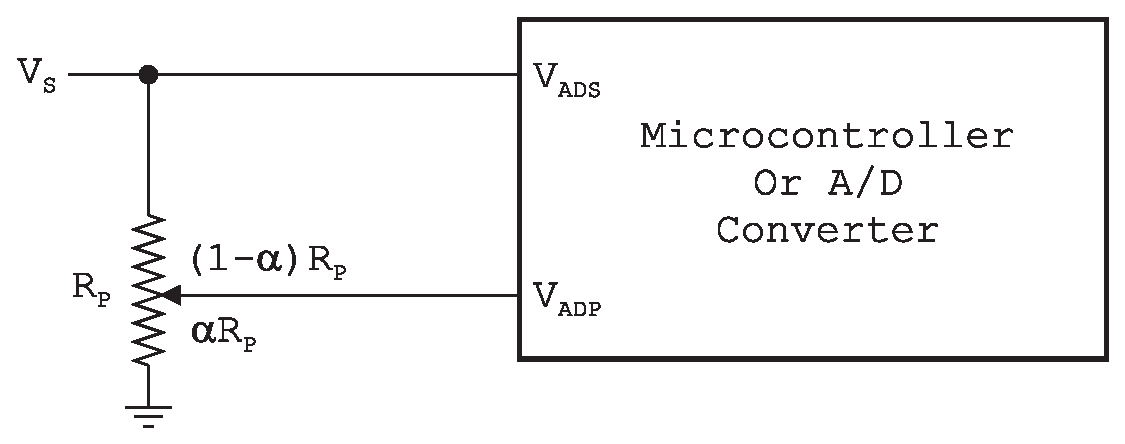
\includegraphics[width=4.6in]{c_soc1/prcs001.eps}
\caption{Prototype Ratiometric Conversion System I}
\label{fig:csoc1:srcs0:soeq0:spsa0:01}
\end{figure}

\begin{table}
\begin{center}
\begin{tabular}{|c|l|}
\hline
Variable           & Description \\
\hline
\hline
$\alpha$           & Potentiometer position, parameterized through $0\leq\alpha\leq 1$. \\
                   & $\alpha=0$ is defined to be the potentiometer position \\
                   & that produces the lowest voltage at the A/D pin, and \\
                   & $\alpha=1$ is defined to be the potentiometer position \\
                   & that produces the highest voltage at the A/D pin.    \\
\hline
$\overline{\alpha}$     
                   & The estimate of potentiometer position, which may    \\
                   & contain error because of quantization error introduced \\
                   & by A/D conversion.                                   \\
\hline
$N_{ADP}$          & The number of A/D counts (supplied to software by an \\
                   & A/D converter) corresponding to the sensing of the   \\
                   & potentiometer position $\alpha$.                     \\
\hline
$\overline{N_{ADP}}$          
                   & $N_{ADP}$ with no quantization error.                \\
\hline
$N_{ADS}$          & The number of A/D counts (supplied to software by an \\
                   & A/D converter) corresponding to the sensing of the   \\
                   & supply voltage $V_S$.                                \\
\hline
$\overline{N_{ADS}}$          
                   & $N_{ADS}$ with no quantization error.                \\
\hline
$R_P$              & The resistance (in Ohms) of the variable potentiometer \\
                   & whose wiper position $\alpha$ is to be sensed (see   \\
                   & Figure~\ref{fig:csoc1:srcs0:soeq0:spsa0:01}).  Note that this resistance does not appear \\
                   & in the analysis of the circuit of Figure~\ref{fig:csoc1:srcs0:soeq0:spsa0:01}, as only  \\
                   & the potentiometer wiper position $\alpha$ affects $V_{ADP}$. \\
\hline
$r_{ADP}$          & The A/D converter ratio (from volts to counts)       \\
                   & implemented by A/D converter monitoring the variable \\
                   & potentiometer input.  Note that $N_P = r_{ADP} V_{ADP}$. \\
\hline
$r_{ADS}$          & The A/D converter ratio (from volts to counts)       \\
                   & implemented by A/D converter monitoring the $V_S$ input. \\
                   & Note that $N_S = r_{ADS} V_{ADS}$.                   \\
\hline
$V_{ADP}$          & The voltage supplied to the microcontroller or A/D   \\
                   & converter corresponding to the variable potentiometer\\
                   & position $\alpha$.  In the system of Figure~\ref{fig:csoc1:srcs0:soeq0:spsa0:01}, $V_{ADP} = \alpha V_S$.\\
\hline
$V_{ADS}$          & The voltage supplied to the microcontroller or A/D   \\
                   & converter corresponding to supply voltage $V_S$.  In \\
                   & the system of Figure~\ref{fig:csoc1:srcs0:soeq0:spsa0:01}, $V_{ADS}=V_S$.  \\
\hline
$V_S$              & The supply voltage, presumed variable, which can be  \\
                   & sensed by the microcontroller software, and also     \\
                   & drives the high side of the variable potentiometer.  \\
\hline
\end{tabular}
\end{center}
\caption{Variables Used In Analysis Of Prototype System I
         (Figure~\ref{fig:csoc1:srcs0:soeq0:spsa0:01})}
\label{tbl:csoc1:srcs0:soeq0:spsa0:01}
\end{table}

To analyze the system depicted in Figure~\ref{fig:csoc1:srcs0:soeq0:spsa0:01},
first note that

\begin{equation}
\label{eq:csoc1:srcs0:soeq0:spsa0:01}
V_{ADS}  =  V_S
\end{equation}

\noindent{}and

\begin{equation}
\label{eq:csoc1:srcs0:soeq0:spsa0:02}
V_{ADP}  =  \alpha V_S.
\end{equation}

For simplicity of analysis, we assume that A/D converters quantize by
truncation, so that

\begin{equation}
\label{eq:csoc1:srcs0:soeq0:spsa0:03}
N_{ADS}  =  \lfloor V_S r_{ADS} \rfloor
\end{equation}

\noindent{}and

\begin{equation}
\label{eq:csoc1:srcs0:soeq0:spsa0:04}
N_{ADP}  =  \lfloor \alpha V_S r_{ADP} \rfloor.
\end{equation}

\noindent{}The assumption that A/D converters quantize by truncation
has little effect on the error analysis of practical systems.  (Need
to include an exercise to show this.)

To aid in symbolic manipulation, we also introduce
$\overline{N_{ADS}}$ and $\overline{N_{ADP}}$, which are
$N_{ADS}$ and $N_{ADP}$, respectively,
without quantization error:

\begin{equation}
\label{eq:csoc1:srcs0:soeq0:spsa0:03b}
\overline{N_{ADS}}  =  V_S r_{ADS}
\end{equation}

\begin{equation}
\label{eq:csoc1:srcs0:soeq0:spsa0:04b}
\overline{N_{ADP}}  =  \alpha V_S r_{ADP}
\end{equation}

If quantization were not present (i.e. if Eqns. 
\ref{eq:csoc1:srcs0:soeq0:spsa0:03}
and 
\ref{eq:csoc1:srcs0:soeq0:spsa0:04}
did not include floor functions), the potentiometer wiper position
$\alpha$ could be calculated exactly as:

\begin{equation}
\label{eq:csoc1:srcs0:soeq0:spsa0:05}
\alpha = \frac{\overline{N_{ADP}} r_{ADS}}{\overline{N_{ADS}} r_{ADP}}.
\end{equation}

Based on (\ref{eq:csoc1:srcs0:soeq0:spsa0:05}),
it makes sense to calculate $\overline{\alpha}$, the
estimate of $\alpha$, as:

\begin{equation}
\label{eq:csoc1:srcs0:soeq0:spsa0:05b}
\overline{\alpha} 
= 
\frac{N_{ADP} r_{ADS}}{N_{ADS} r_{ADP}}.
\end{equation}

The question that must be posed is:
\emph{How different from $\alpha$ can $\overline{\alpha}$ be?}.
We seek to bound $|\overline{\alpha}-\alpha|$.

Quantization can be treated by noting that applying the floor function
to an input introduces an error $\in (-1,0]$, i.e.

\begin{equation}
\label{eq:csoc1:srcs0:soeq0:spsa0:06}
\lfloor x \rfloor = x + \varepsilon; \;\; \varepsilon \in  (-1,0].
\end{equation}

Using this observation, we can rewrite
(\ref{eq:csoc1:srcs0:soeq0:spsa0:05b}) as

\begin{equation}
\label{eq:csoc1:srcs0:soeq0:spsa0:07}
\overline{\alpha} 
= 
\frac{N_{ADP} r_{ADS}}{N_{ADS} r_{ADP}}
=
\frac{(\overline{N_{ADP}} + \varepsilon_1) r_{ADS}}{(\overline{N_{ADS}} + \varepsilon_2) r_{ADP}} ;
\;\;
\varepsilon_1, \varepsilon_2 \in (-1, 0].
\end{equation}

\noindent{}It can be seen from
(\ref{eq:csoc1:srcs0:soeq0:spsa0:07})
that the minimum value of the estimate 
$\overline{\alpha}$ occurs when $\varepsilon_1$ is minimized and 
$\varepsilon_2$ is maximized.  Similarly, the maximum 
value occurs when $\varepsilon_1$ is maximized and 
$\varepsilon_2$ is minimized.  These observations lead to this
inequality:

\begin{equation}
\label{eq:csoc1:srcs0:soeq0:spsa0:08}
\frac{N_{ADP} r_{ADS}}{(N_{ADS}+1) r_{ADP}}
<
\alpha
<
\frac{(N_{ADP}+1) r_{ADS}}{r_{ADP}} .
\end{equation}

Intuitively, the form of (\ref{eq:csoc1:srcs0:soeq0:spsa0:08})
makes sense.  The smallest possible value of $\alpha$ will correspond
to the case
when $N_{ADP}$ contains no quantization error but $N_{ADS}$ contains
a quantization error of nearly 1.
The largest possible value of $\alpha$ will correspond
to the case
when $N_{ADS}$ contains no quantization error but $N_{ADP}$ contains
a quantization error of nearly 1.

It can also be seen from (\ref{eq:csoc1:srcs0:soeq0:spsa0:08}) that
the interval to which $\alpha$ is confined will be larger
when $V_S$ is smaller (implying a smaller $N_{ADS}$ and $N_{ADP}$).
This is also intuitively plausible, since the quantization error 
of up to one count in $N_{ADS}$ or $N_{ADP}$ will have a larger
relative significance when $N_{ADS}$ and $N_{ADP}$ are smaller.

The inequality provided in (\ref{eq:csoc1:srcs0:soeq0:spsa0:08})
is certainly useful, and gives insight into quantization error.  However,
we seek an inequality that is more friendly to engineering work, i.e.
one that involves voltages rather than A/D counts.

Assume it is known for an application that $V_S$ can vary only over the
interval

\begin{equation}
\label{eq:csoc1:srcs0:soeq0:spsa0:08b}
V_S \in [V_{SMIN}, V_{SMAX}], 
\end{equation}


\noindent{}and that $\alpha$ can very only over
the interval 

\begin{equation}
\label{eq:csoc1:srcs0:soeq0:spsa0:08c}
\alpha \in [\alpha_{MIN}, \alpha_{MAX}].
\end{equation}

\noindent{}Furthermore, we
seek useful inequalities where is it \emph{not} required 
that\footnote{(\ref{eq:csoc1:srcs0:soeq0:spsa0:09}) represents the 
requirement that $V_{SMIN}$ or $V_{SMAX}$ represent a precisely 
integral number of A/D
counts.  This requirement is almost never met in practical engineering
work.}

\begin{equation}
\label{eq:csoc1:srcs0:soeq0:spsa0:09}
r_{ADS} \vworkdivides \{V_{SMIN},V_{SMAX}\},
\end{equation}

\noindent{}as if (\ref{eq:csoc1:srcs0:soeq0:spsa0:09})
were required, it would introduce extra complexity 
in applying the inequality.

To develop the desired type of inequality, we can use
a different analysis method.  Assume that 
$r_{ADS}$ and $r_{ADP}$ are fixed.  Then, introduce
the function

\begin{equation}
\label{eq:csoc1:srcs0:soeq0:spsa0:10}
F(\overline{N_{ADP}}, \overline{N_{ADS}}) 
= 
\frac{\overline{N_{ADP}} r_{ADS}}{\overline{N_{ADS}} r_{ADP}},
\end{equation}

\noindent{}which, in accordance with (\ref{eq:csoc1:srcs0:soeq0:spsa0:05}),
is a perfect estimate of $\alpha$.

\begin{figure}
\centering
\Huge{TBD}
\caption{Sample Staircase Pattern Of Estimate $\overline{\alpha}$ Of
         Prototype Ratiometric Conversion System I}
\label{fig:csoc1:srcs0:soeq0:spsa0:02}
\end{figure}

We can examine the staircase pattern of $\overline{\alpha}$ as 
$V_S$ is increased (see Figure \ref{fig:csoc1:srcs0:soeq0:spsa0:02},
which provides an example staircase pattern).  Note that the staircase
pattern may contain four qualitatively
distinct types of vertical discontinuities.  In the descriptions below,
assume that $V_D \in [V_{SMIN}, V_{SMAX}]$ is the value of
$V_S$ at the discontinuity.

\begin{itemize}
\item \textbf{Downward overshoot discontinuities (DOD):}
      As $V_S$ is increased, these correspond to the values
      of $V_S$ where $V_S r_{ADS} \in \vworkintset$ but
      $V_S \alpha r_{ADS} \notin \vworkintset$.  At such 
      discontinuities, 
      $\lim_{V_S \rightarrow V_D^-}\overline{\alpha} > \alpha$,
      but 
      $\lim_{V_S \rightarrow V_D^+}\overline{\alpha} < \alpha$.
\item \textbf{Upward overshoot discontinuities (UOD):}
      As $V_S$ is increased, these correspond to the values
      of $V_S$ where $V_S r_{ADS} \notin \vworkintset$ but
      $V_S \alpha r_{ADS} \in \vworkintset$.  At such 
      discontinuities, 
      $\lim_{V_S \rightarrow V_D^-}\overline{\alpha} < \alpha$,
      but 
      $\lim_{V_S \rightarrow V_D^+}\overline{\alpha} > \alpha$.
\item \textbf{Downward exact discontinuities (DED):}
      As $V_S$ is increased, these correspond to the values
      of $V_S$ where $V_S r_{ADS} \in \vworkintset$ and
      $V_S \alpha r_{ADS} \in \vworkintset$.  At such 
      discontinuities, 
      $\lim_{V_S \rightarrow V_D^-}\overline{\alpha} > \alpha$,
      but 
      $\lim_{V_S \rightarrow V_D^+}\overline{\alpha} = \alpha$.
\item \textbf{Upward exact discontinuities (UED):}
      As $V_S$ is increased, these correspond to the values
      of $V_S$ where $V_S r_{ADS} \in \vworkintset$ and
      $V_S \alpha r_{ADS} \in \vworkintset$.  At such 
      discontinuities, 
      $\lim_{V_S \rightarrow V_D^-}\overline{\alpha} < \alpha$,
      but 
      $\lim_{V_S \rightarrow V_D^+}\overline{\alpha} = \alpha$.
\end{itemize}

We can place upper bounds on the magnitudes of the discontinuities
by examining the partial derivatives of
$F(\overline{N_{ADP}}, \overline{N_{ADS}})$ as specified in
(\ref{eq:csoc1:srcs0:soeq0:spsa0:10}), specifically:

\begin{equation}
\label{eq:csoc1:srcs0:soeq0:spsa0:11}
\frac{\partial{}F(\cdot{},\cdot{})}{\partial \overline{N_{ADS}}}
= 
-
\frac{\overline{N_{ADP}} r_{ADS}}{\overline{N_{ADS}^2} r_{ADP}}
\end{equation}

\begin{equation}
\label{eq:csoc1:srcs0:soeq0:spsa0:11b}
\frac{\partial{}^2 F(\cdot{},\cdot{})}{\partial \overline{N_{ADS}}^2}
= 
2
\frac{\overline{N_{ADP}} r_{ADS}}{\overline{N_{ADS}^3} r_{ADP}}
\end{equation}

\begin{equation}
\label{eq:csoc1:srcs0:soeq0:spsa0:11c}
\frac{\partial{}^i F(\cdot{},\cdot{})}{\partial \overline{N_{ADS}}^i}
= 
(-1)^i (i!)
\frac{\overline{N_{ADP}} r_{ADS}}{\overline{N_{ADS}^{i+1}} r_{ADP}}
\end{equation}


\begin{equation}
\label{eq:csoc1:srcs0:soeq0:spsa0:12}
\frac{\partial{}F(\cdot{},\cdot{})}{\partial \overline{N_{ADP}}}
= 
-
\frac{r_{ADS}}{\overline{N_{ADS}} r_{ADP}}
\end{equation}

\begin{equation}
\label{eq:csoc1:srcs0:soeq0:spsa0:12b}
\frac{\partial{}^i F(\cdot{},\cdot{})}{\partial \overline{N_{ADP}}^i}
= 
0, \; i \geq 2
\end{equation}

A \emph{DOD} (discussed above) corresponds to the case where
$N_{ADS}$ increases by one count at $V_S=V_D$ without an increase in
$N_{ADP}$.    


A \emph{UOD} (discussed above) corresponds to the case where
$N_{ADP}$ increases by one count at $V_S=V_D$ without an increase in
$N_{ADS}$.    




%%%%%%%%%%%%%%%%%%%%%%%%%%%%%%%%%%%%%%%%%%%%%%%%%%%%%%%%%%%%%%%%%%%%%%%%%%
%%%%%%%%%%%%%%%%%%%%%%%%%%%%%%%%%%%%%%%%%%%%%%%%%%%%%%%%%%%%%%%%%%%%%%%%%%
%%%%%%%%%%%%%%%%%%%%%%%%%%%%%%%%%%%%%%%%%%%%%%%%%%%%%%%%%%%%%%%%%%%%%%%%%%
\section{Motion Control Systems}


%%%%%%%%%%%%%%%%%%%%%%%%%%%%%%%%%%%%%%%%%%%%%%%%%%%%%%%%%%%%%%%%%%%%%%%%%%
\vfill
\noindent\begin{figure}[!b]
\noindent\rule[-0.25in]{\textwidth}{1pt}
\begin{tiny}
\begin{verbatim}
$HeadURL: svn://localhost/dtapublic/pubs/books/ucbka/trunk/c_soc1/c_soc1.tex $
$Revision: 279 $
$Date: 2019-08-16 23:10:13 -0400 (Fri, 16 Aug 2019) $
$Author: dashley $
\end{verbatim}
\end{tiny}
\noindent\rule[0.25in]{\textwidth}{1pt}
\end{figure}
%%%%%%%%%%%%%%%%%%%%%%%%%%%%%%%%%%%%%%%%%%%%%%%%%%%%%%%%%%%%%%%%%%%%%%%%%%
%
%End of file C_PCO0.TEX


%Chapter:  Support Of Communication Protocols And Networks
\chapter{\csnczerolongtitle{}}

\label{csnc0}

\beginchapterquote{``Under construction!''}
                     {Under construction!}

\section{Introduction}
%Section tag: INT0

%End of file c_snc0.tex



%Chapter:  Support Of Frequently-Occurring Requirements
\chapter{\csfozerolongtitle{}}

\label{csfo0}

\beginchapterquote{``Under construction!''}
                     {Under construction!}

\section{Introduction}
%Section tag: INT0


%%%%%%%%%%%%%%%%%%%%%%%%%%%%%%%%%%%%%%%%%%%%%%%%%%%%%%%%%%%%%%%%%%%%%%%%%%
%End of file c_sfo0.tex


%Chapter:  Real-Time Analysis
%$Header: svn://localhost/dtapublic/pubs/books/ucbka/trunk/c_rta0/c_rta0.tex 278 2019-08-14 23:10:36Z dashley $

\chapter{\crtazerolongtitle{}}

\label{crta0}

\beginchapterquote{``Under construction!''}
                     {Under construction!}

\section{Introduction}
%Section tag: INT0



%%%%%%%%%%%%%%%%%%%%%%%%%%%%%%%%%%%%%%%%%%%%%%%%%%%%%%%%%%%%%%%%%%%%%%%%%%
\vfill
\noindent\begin{figure}[!b]
\noindent\rule[-0.25in]{\textwidth}{1pt}
\begin{tiny}
\begin{verbatim}
$HeadURL: svn://localhost/dtapublic/pubs/books/ucbka/trunk/c_rta0/c_rta0.tex $
$Revision: 278 $
$Date: 2019-08-14 19:10:36 -0400 (Wed, 14 Aug 2019) $
$Author: dashley $
\end{verbatim}
\end{tiny}
\noindent\rule[0.25in]{\textwidth}{1pt}
\end{figure}
%%%%%%%%%%%%%%%%%%%%%%%%%%%%%%%%%%%%%%%%%%%%%%%%%%%%%%%%%%%%%%%%%%%%%%%%%%
%
%End of file C_PCO0.TEX


% New part: Embedded System Algorithms And Techniques
\part{Embedded System Algorithms And Techniques}

%Chapter:  Classical And Simple Integer Algorithms And Techniques
%$Header: svn://localhost/dtapublic/pubs/books/ucbka/trunk/c_cil0/c_cil0.tex 277 2019-08-13 02:35:39Z dashley $

\chapter[\ccilzeroshorttitle{}]{\ccilzerolongtitle{}}

\label{ccil0}

\beginchapterquote{``If our ancestors had invented arithmetic by counting with
                     their two fists or their eight fingers, instead of their
                     ten `digits', we would never have to worry about
                     writing binary-decimal conversion routines.
                     (And we would perhaps never have learned as much about
                     number systems.)''}
                     {Donald E. Knuth, \cite[p. 319]{bibref:b:knuthclassic2ndedvol2}}

%%%%%%%%%%%%%%%%%%%%%%%%%%%%%%%%%%%%%%%%%%%%%%%%%%%%%%%%%%%%%%%%%%%%%%%%%%
%%%%%%%%%%%%%%%%%%%%%%%%%%%%%%%%%%%%%%%%%%%%%%%%%%%%%%%%%%%%%%%%%%%%%%%%%%
%%%%%%%%%%%%%%%%%%%%%%%%%%%%%%%%%%%%%%%%%%%%%%%%%%%%%%%%%%%%%%%%%%%%%%%%%%
\section{Introduction}
%Section tag: INT0
\label{ccil0:sint0}

Low-cost microcontrollers have no support for floating-point arithmetic,
and so integer arithmetic and fixed-point arithmetic are used nearly exclusively
in embedded systems.  The ability to implement integer arithmetic
economically is a critical skill in the development of embedded
systems.

Integer arithmetic algorithms are critically important in embedded
systems for the following reasons:

\begin{itemize}
\item Mistakes in the implementation of arithmetic are frequently
      responsible for product problems.  (Mistakes are not confined
      to obvious errors---errors such as filters which do not converge
      on their input are also responsible for product problems.)
\item Floating-point arithmetic is not available or ill-advised
      for nearly all small embedded systems for the following reasons:
      \begin{itemize}
      \item Low-cost microcontrollers do not possess hardware support for
            floating-point arithmetic.
      \item Implementation of floating-point arithmetic in software is
            computationally expensive.
      \item Implementation of floating-point arithmetic in software may
            require large floating-point libraries, typically consuming
            1K-4K of ROM.
      \item Safety-critical software standards typically prohibit the
            use of floating-point arithmetic.
      \end{itemize}
\item Integer arithmetic algorithms (other than addition and subtraction)
      are quite tedious and error-prone for a software developer to design, implement, and
      unit test.  The implementation of such algorithms represents
      cost and risk.  Cost and risk benefits are achieved if the algorithms in detail are 
      available in advance (thus precluding design activities), or
      better yet if ready-to-use integer algorithm libraries are available.
\end{itemize}

This chapter describes the more fundamental principles and algorithms
(representation, fixed-point arithmetic, treatment of overflow, comparison,
addition, subtraction, multiplication, and division).  A section 
(Section \ref{ccil0:smim0}) is also included 
on miscellaneous mappings involving integers which
are not numerical in intent.
Chapter %\cdtazeroxrefhyphen\cdtazerovolarabic{} 
TBD
describes more complicated 
integer algorithms and techniques (discrete-time operations
such as filtering, integration, and differentiation as well as more
complex functions such as square root).  The split between these two chapters
is arbitrary; and in fact the material could have been divided differently
or combined.

Treatment of the topics in this chapter is largely in accordance with
Knuth \cite{bibref:b:knuthclassic2ndedvol2}.  The principal issues in 
the implementation of integer algorithms are:

\begin{itemize}
\item \textbf{How to use the arithmetic [or other] instructions provided by the machine to
      operate on larger operands.}  Microcontrollers typically provide arithmetic
      instructions (comparison, shifting, addition, subtraction, and often but not
      always multiplication and/or division) that operate on 8-bit or 16-bit integers.  
      A key question
      is how small-operand instructions ``scale up''---that is, if and how they can
      be used to assist in the implementation of integer arithmetic for much larger 
      operands.
\item \textbf{The order of the algorithm involved.}  The order of algorithms
      is a complicated issue when applied to microcontroller work.  Many sophisticated
      algorithms have a breakpoint below which they are less economical than
      an inferior algorithm.  Some applications (such as generating cryptographic keys
      when integers thousands of bits long must be tested for primality) will
      benefit from sophisticated algorithms becuase the operand sizes are large enough
      to pass any such breakpoints.  However, in microcontroller work, the need to manipulate
      integers longer than 64 bits is very rare; thus, the breakpoints that indicate the
      use of more sophisticated algorithms may not be reached.  In microcontroller work,
      depending on the operand sizes, there are circumstances in which an
      $O(n^2)$ algorithm may be preferable to an $O(\log n)$ algorithm.  Generally,
      the order of algorithms must be balanced against operand sizes.
\end{itemize}

We do diverge from Knuth in some areas.  The most prominent divergence is
in the proofs offered for some important theorems and lemmas.  Knuth 
employs contrapositive proof formats in many circumstances, whereas we prefer
to use linear proofs that are more understandable to engineers and microcontroller
software developers.

%%%%%%%%%%%%%%%%%%%%%%%%%%%%%%%%%%%%%%%%%%%%%%%%%%%%%%%%%%%%%%%%%%%%%%%%%%
%%%%%%%%%%%%%%%%%%%%%%%%%%%%%%%%%%%%%%%%%%%%%%%%%%%%%%%%%%%%%%%%%%%%%%%%%%
%%%%%%%%%%%%%%%%%%%%%%%%%%%%%%%%%%%%%%%%%%%%%%%%%%%%%%%%%%%%%%%%%%%%%%%%%%
\section[Paradigms And Principles]
        {Paradigms And Principles Of Microcontroller Arithmetic}
%Section tag: PPM0
\label{ccil0:sppm0}

How should one think about microcontroller arithmetic?  What principles
guide us in its design and implementation?  In this section,
we provide some general principles and paradigms of thought.


%%%%%%%%%%%%%%%%%%%%%%%%%%%%%%%%%%%%%%%%%%%%%%%%%%%%%%%%%%%%%%%%%%%%%%%%%%
%%%%%%%%%%%%%%%%%%%%%%%%%%%%%%%%%%%%%%%%%%%%%%%%%%%%%%%%%%%%%%%%%%%%%%%%%%
%%%%%%%%%%%%%%%%%%%%%%%%%%%%%%%%%%%%%%%%%%%%%%%%%%%%%%%%%%%%%%%%%%%%%%%%%%
\subsection{Microcontroller Arithmetic As An Accident Of Silicon Design}
%Subsection tag: MAS0
\label{ccil0:sppm0:smas0}

In chapters
\cfryzeroxrefhyphen{}\ref{cfry0},
\ccfrzeroxrefhyphen{}\ref{ccfr0},
and 
\cratzeroxrefhyphen{}\ref{crat0} 
we consider rational approximation,
both in the form $h/k$ and $h/2^q$.  Both forms of rational approximation
tend to be effective because we know that all modern processors possess
shift instructions, most possess integer multiply instructions, and many 
possess integer divide instructions.  In other words, the design
of the machine instruction set drives the strategies for implementation
of arithmetic, and makes some strategies attractive.

Similarly, the observation that all microcontrollers provide instructions
for integer arithmetic creates the attractiveness of fixed-point arithmetic.

Thus, we might view our approaches to microcontroller arithmetic as 
an ``accident'' of silicon design, or as being driven by silicon
design.

Generally, we seek to determine the best way to use the primitive
operations provided by the machine (the instruction set) to 
accomplish the mappings of interest.

The ``classic'' algorithms 
presented by Knuth 
Knuth (\cite[pp. 265-284]{bibref:b:knuthclassic2ndedvol2}) are especially
designed to use the ``small'' addition, subtraction, multiplication, and
division provided by the machine to add, subtract, multiply, and divide arbitrarily
large integers.  In 
\cite[pp. 265-266]{bibref:b:knuthclassic2ndedvol2}) Knuth writes:

\begin{quote}
\emph{The most important fact to understand about extended-precision numbers
is that they may be regarded as numbers written in radix-$w$ notation,
where $w$ is the computer's word size.  For example, an integer that
fills 10 words on a computer whose word size is $w=10^{10}$ has 100
decimal digits; but we will consider it to be a 10-place number to
the base $10^{10}$.  This viewpoint is justified for the same reason
that we may convert, say, from binary to hexadecimal notation,
simply by grouping the bits together.}

\emph{In these terms, we are given the following primitive operations to work with:}

\begin{itemize}
\item \emph{a$_0$) addition or subtraction of one-place integers, giving a one-place
             answer and a carry;}
\item \emph{b$_0$) multiplication of a one-place integer by another one-place integer,
             giving a two place answer;}
\item \emph{c$_0$) division of a two-place integer by a one-place integer, 
             provided that the quotient is a one-place integer, and yielding
			    also a one-place remainder.}
\end{itemize}

\noindent{}\emph{By adjusting the word size, if necessary, nearly all computers
will have these three operations available; so we will construct algorithms
(a), (b), and (c) mentioned above in terms of the primitive operations
(a$_0$), (b$_0$), and (c$_0$).}

\emph{Since we are visualizing extended-precision integers as base $b$ numbers, it is
sometimes helpful to think of the situation when $b = 10$, and to imagine
that we are doing the arithmetic by hand.  Then operation (a$_0$) is analogous
to memorizing the addition table; (b$_0$) is analogous to memorizing the 
multiplication table, and (c$_0$) is essentially memorizing the multiplication
table in reverse.  The more complicated operations (a), (b), (c) on
high-precision numbers can now be done using simple addition, subraction,
multiplication, and long-division procedures that children are taught
in elementary school.}
\end{quote}

The critical issue for implementation of integer arithmetic with large operands
is how to use small-operand instructions to operate on larger operands---in other words,
how to ``scale up'' the capability provided by the instruction set. 


%%%%%%%%%%%%%%%%%%%%%%%%%%%%%%%%%%%%%%%%%%%%%%%%%%%%%%%%%%%%%%%%%%%%%%%%%%
%%%%%%%%%%%%%%%%%%%%%%%%%%%%%%%%%%%%%%%%%%%%%%%%%%%%%%%%%%%%%%%%%%%%%%%%%%
%%%%%%%%%%%%%%%%%%%%%%%%%%%%%%%%%%%%%%%%%%%%%%%%%%%%%%%%%%%%%%%%%%%%%%%%%%
\subsection{Microcontroller Arithmetic As A Mapping From Quantized Domain To
            Quantized Range}
%Subsection tag: MAM0
\label{ccil0:sppm0:smam0}

Microcontroller software accepts inputs which are quantized.  In nearly all cases,
this involves a mapping from $\vworkrealset$ to $\vworkintset$.  Often, because
microcontroller products are optimized for cost, the quantization hardware
delivers quite poor precision, frequently less than 8 bits.  

When a quantized input is accepted, it defines an inquality.  Knowledge of
the quantized input (an integer) confines the actual input (a real
number, before 
quantization) to an interval.  With a low-cost hardware design, the
interval can be fairly large.  Usually, by adding cost, the
interval can be made smaller.

Microcontroller outputs tend to be quantized as well, so it is
accurate to also characterize outputs as integers.  For example, a PWM signal
generated by a microcontroller or the output of a D/A converter is
controlled by data that is an integer.  Like inputs, often the ``granularity''
with which outputs can be controlled is quite coarse---again, 8 bits or
less is not uncommon.

Thus, we may view microcontroller software as a mapping from poor-quality
inputs to poor-quality outputs.

In such a framework, where the nature of inputs and outputs introduces
substantial error, it is imperative not to introduce additional error
in computer arithmetic.  In other words, given inputs which are 
integers, the responsibility of the software is to choose the best 
integers as outputs.  Usually this means that calculations should be
devised so as not to lose any information (i.e.
not to lose remainders, for example).  Losing information is usually
equivalent to not being able to make the most correct mapping from input
to output.  ``Lossy'' arithmetic can degrade the performance of a system,
since poor arithmetic may compound an inexpensive hardware design.


%%%%%%%%%%%%%%%%%%%%%%%%%%%%%%%%%%%%%%%%%%%%%%%%%%%%%%%%%%%%%%%%%%%%%%%%%%
%%%%%%%%%%%%%%%%%%%%%%%%%%%%%%%%%%%%%%%%%%%%%%%%%%%%%%%%%%%%%%%%%%%%%%%%%%
%%%%%%%%%%%%%%%%%%%%%%%%%%%%%%%%%%%%%%%%%%%%%%%%%%%%%%%%%%%%%%%%%%%%%%%%%%
\subsection{Microcontroller Arithmetic As A Simulation Of Continuous Controllers}
%Subsection tag: MAE0
\label{ccil0:sppm0:smae0}

Control systems have not always employed digital controllers.
Many books and web sites (see \cite{bibref:w:historycontrol01}, for example)
discuss the historical development of feedback control.  Controllers
have not historically been digital, or even electronic.
Early controllers for governing steam devices or windmills were
ultimately mechanical, and relied upon inertia or other physical
properties.  It is possible to realize abstract notions
(integrators, differentiators, gains) using hydraulic systems or other mechanical systems;
and in fact hydraulic feedback controllers were used in early rockets
and aircraft.  Very naturally, abstract notions (integrators,
differentiators, gains) can be implemented using analog
electronic components.  The most common implementations involve
operational amplifiers, and the behavior of such implementations comes
very close to the ideal mathematical models.

Mechanical, hydraulic, and non-digital electronic controllers have
one very desirable characteristic---\emph{clipping}.  If, for example,
one provides an analog differentiator with a $dV/dt$ which
is too large, the output that the differentiator can 
provide is limited, usually by the supply voltage available to an operational
amplifier.
The differentiator \emph{must} clip.

Clipping often leads to behavior which is close to what
intuition would expect (i.e. we would present 
clipping as an occasional advantage).  For example, if an input to
an analog control system suffers a failure, the behavior
the of the controller is limited, as is its internal
state.  Similarly, when the
input is restored, the controller will usually recover 
in a reasonable time because the
state of the controller (typically maintained in capacitors) is limited
in the magnitude it can attain.

We might view a digital controller as an emulation of
an analog controller.  We may want to cause the
controller to have limits (i.e. rails) internally, for
example to prevent excessive integrator ``windup''.  We discuss
this further in Section \ref{ccil0:sode0}.


%%%%%%%%%%%%%%%%%%%%%%%%%%%%%%%%%%%%%%%%%%%%%%%%%%%%%%%%%%%%%%%%%%%%%%%%%%
%%%%%%%%%%%%%%%%%%%%%%%%%%%%%%%%%%%%%%%%%%%%%%%%%%%%%%%%%%%%%%%%%%%%%%%%%%
%%%%%%%%%%%%%%%%%%%%%%%%%%%%%%%%%%%%%%%%%%%%%%%%%%%%%%%%%%%%%%%%%%%%%%%%%%
\section{Practical Design Issues}
%Section tag: PDI0
\label{ccil0:spdi0}

In this section, we consider practical issues surrounding the design
and construction of a set of integer arithmetic subroutines.
In practice, such a collection of subroutines is likely to be
arranged into a library.  The purpose of the library would be to
free the clients (or callers) of the library from the complexity of 
large integer calculations.

The design decisions surrounding the construction of a library vary in
the objectivity with which they can be approached.  Some design decisions
(such as the best mechanism for passing parameters) can be approached
rigorously because the measures of goodness are unequivocal (minimal ROM consumption
or execution time, for example).  However, other design decisions, particulary the
decision of the exact nature of the interface between an arithmetic library and
its clients, are more subjective.  One size does \emph{not} fit all.


%%%%%%%%%%%%%%%%%%%%%%%%%%%%%%%%%%%%%%%%%%%%%%%%%%%%%%%%%%%%%%%%%%%%%%%%%%
%%%%%%%%%%%%%%%%%%%%%%%%%%%%%%%%%%%%%%%%%%%%%%%%%%%%%%%%%%%%%%%%%%%%%%%%%%
%%%%%%%%%%%%%%%%%%%%%%%%%%%%%%%%%%%%%%%%%%%%%%%%%%%%%%%%%%%%%%%%%%%%%%%%%%
\subsection{Parameter Passing And Temporary Storage Mechanisms}
%Subsection tag: PPM0
\label{ccil0:spdi0:sppm0}

In small microcontroller work, the desire to save ROM and execution time
may lead to inelegant software construction.  Because an arithmetic library
used in microcontroller work may be called from many different places 
throughout ROM, serious thought should be given to optimizing the 
parameter passing mechanisms, even perhaps at the expense of elegance.
The way in which the arithmetic library allocates temporary storage is
also a point of concern, because the most elegant way of allocating temporary
storage (on the stack) may either not be feasible (because of the possibility
of stack overflow) or may not be efficient (because the addressing modes of
the machine make data on the stack inefficient to address).  In this section
we discuss both parameter passing and temporary storage mechanisms.

In the remainder of the discussion, we make the following assumptions
about software architecture.

\begin{enumerate}
\item \textbf{The arithmetic library need not be re-entrant.}
      Most ``small'' microcontroller software loads use a non-preemptive
      scheduling paradigm, so this is a reasonable assumption.  We also
      make the reasonable assumption that ISR's may not make calls into 
      the arithmetic library.
\item \textbf{Dynamic memory allocation, other than on the stack,
      is not allowed by the software architecture.}  This is also
      a reasonable assumption in ``small'' microcontroller software.
\end{enumerate}

%%%%%%%%%%%%%%%%%%%%%%%%%%%%%%%%%%%%%%%%%%%%%%%%%%%%%%%%%%%%%%%%%%%%%%%%%%
%%%%%%%%%%%%%%%%%%%%%%%%%%%%%%%%%%%%%%%%%%%%%%%%%%%%%%%%%%%%%%%%%%%%%%%%%%
%%%%%%%%%%%%%%%%%%%%%%%%%%%%%%%%%%%%%%%%%%%%%%%%%%%%%%%%%%%%%%%%%%%%%%%%%%
\subsubsection{Parameter Passing Mechanisms}
%Subsubsection tag: PPM0
\label{ccil0:spdi0:sppm0:sppm0}

If an arithmetic library exists in a microcontroller software load,
it may be called many times throughout ROM.  Thus, the parameter 
passing mechanisms chosen may have a large effect on ROM consumption
(due to the setup required for each subroutine call multiplied by
many instances throughout ROM) and execution time
(because in microcontroller software longer instructions nearly always
require more time).  Because of the criticality of ROM consumption,
parameter passing mechanisms that lack elegance may be attractive.

In the category of parameter passing, we also include the way in which
return value(s) are passed back to the caller.

The following parameter-passing mechanisms may be employed:

\begin{enumerate}
\item \textbf{Pass by value as storage class \emph{automatic}.}
      The most common scenario is that the arithmetic
      library is written in assembly-language to be called from
      `C', and so the assembly-language subroutines must adhere to the
      parameter-passing conventions used by the compiler.
      This usually means that the entire input or output value
      will be passed in CPU registers or on the stack.  Somewhat rarely, 
      a compiler will pass parameters in static locations.\footnote{The
      usual reason for a `C' compiler to pass parameters in static locations
      is because the instruction set of the machine was not designed for
      higher-level languages, and references to [usually \emph{near}] memory
      are cheaper than stack references.  Such compilers also typically 
      analyze the calling tree of the program where possible and use this
      information to overlay the parameter-passing memory areas of 
      subroutines that cannot be active simultaneously.  Without the ability
      to analyze the calling tree and make overlay decisions based on it,
      memory would be exhausted, because each subroutine would need to have its
      own static storage for parameters and local variables.}
\item \textbf{Pass by reference.}
      Typically, it is convenient to pass pointer(s) to area(s) of memory
      containing input operands, and also a pointer to an area of memory
      owned by the caller which is written with the result by the arithmetic subroutine.
      The efficiency of this approach depends on the compiler and the instruction
      set of the machine.  If the instruction set of the machine cannot 
      make effective use of pointers or stack frames, an arithmetic subroutine
      might be constructed so that it first copies the operands to a static area of memory
      reserved for the arithmetic library, then performs the necessary arithmetic
      operations on the operands in the static area, 
      then copies the result(s) back to the area owned by the caller.
\item \textbf{Pass by common data block.}
      In some cases, it may be preferable to reserve a block of memory in which to
      pass parameters to arithmetic library functions, and from which to retrieve
      results after an arithmetic library function returns.  The allocation of such
      a static memory block may be done manually\footnote{Note to self:  need to
      include gentleman's agreements on memory usage in my note on software architecture.}
      or automatically (by development tools which can analyze the function calling tree and
      manage the overlaying).
\end{enumerate}



%%%%%%%%%%%%%%%%%%%%%%%%%%%%%%%%%%%%%%%%%%%%%%%%%%%%%%%%%%%%%%%%%%%%%%%%%%
%%%%%%%%%%%%%%%%%%%%%%%%%%%%%%%%%%%%%%%%%%%%%%%%%%%%%%%%%%%%%%%%%%%%%%%%%%
%%%%%%%%%%%%%%%%%%%%%%%%%%%%%%%%%%%%%%%%%%%%%%%%%%%%%%%%%%%%%%%%%%%%%%%%%%
\subsubsection{Temporary Storage Mechanisms}
%Subsubsection tag: TSM0
\label{ccil0:spdi0:sppm0:stsm0}

Need to indicate clearly on section on software architectures the
primary temporary storage mechanisms:

\begin{itemize}
\item Stack.
\item Memory block with overlay functionality.
\end{itemize}

Need to expand software architecture section to cover this, so don't
discuss here.


%%%%%%%%%%%%%%%%%%%%%%%%%%%%%%%%%%%%%%%%%%%%%%%%%%%%%%%%%%%%%%%%%%%%%%%%%%
%%%%%%%%%%%%%%%%%%%%%%%%%%%%%%%%%%%%%%%%%%%%%%%%%%%%%%%%%%%%%%%%%%%%%%%%%%
%%%%%%%%%%%%%%%%%%%%%%%%%%%%%%%%%%%%%%%%%%%%%%%%%%%%%%%%%%%%%%%%%%%%%%%%%%
\subsection{Reporting Of Overflow, Underflow, And Domain Errors}
%Subsection tag: OUD0
\label{ccil0:spdi0:soud0}

Long integer data types used in microcontroller work are typically
of a static size (they cannot grow in size in as operations are 
performed on them).  The reason for the typical static sizes is that
dynamic allocation (except for allocation and
deallocation on the stack as subroutines
are called and return) is rarely used in small microcontroller work.
It will come about in the normal usage of an integer arithmetic 
library that an attempt will be made to operate on integers in
a way which generates an overflow, generates an
underflow, or
represents a domain error (division by zero or
square root of a negative integer, for example).
An important design decision is how such normal exceptions should be
handled.

Possible design decisions in this area are:

\begin{enumerate}
\item \label{enum:ccil0:spdi0:soud0:01:01}
      \textbf{To design arithmetic subroutines so that exceptions are not
      possible.}  
      For example, multiplying an $m$-word integer by an $n$-word integer
      will always generate an integer that will fit within $m+n$ words.
      If a multiplication subroutine is designed so that the caller must
      provide an $m$-word operand and an $n$-word operand and a pointer to
      an $(m+n)$-word area of memory for the result, an overflow cannot occur.
      Such a design decision essentially pushes overflow detection back up to
      the callers of arithmetic subroutines.
\item \label{enum:ccil0:spdi0:soud0:01:02}
      \textbf{To design arithmetic subroutines so that exceptions are possible,
      but not to detect the exceptions, thus providing an implementation that
      will produce incorrect results with some operand data values.}
      For example, if an arithmetic subroutine is designed to add an $m$-word
      operand to another $m$-word operand to produce an $m$-word result, overflow
      is possible.  A design decision to fail to detect such exceptions pushes
      the responsibility up to the callers of the arithmetic subroutines.
      Callers must devise a method for not calling arithmetic subroutines
      with data values that will cause an exception, or else to detect an exception
      when it has occurred.
\item \label{enum:ccil0:spdi0:soud0:01:03}
      \textbf{To ``rail'' the result in response to an exception.}  
      It was stated earlier that analog control system functional blocks
      built with operational 
      amplifiers typically have an output which cannot go beyond the 
      supply rails.  One may implement similar behavior in arithmetic subroutines.
      In an addition subroutine which adds two $m$-word operands to produce an
      $m$-word result (with each word having $w$ bits), it would be natural to 
      return $2^{mw}-1$ in the event of an overflow in a positive direction and 
      $-2^{mw}$ in the event of an overlfow in a negative direction.  Note that
      the caller will not be able to distinguish a ``rail'' value which represents
      a valid result from a ``rail'' value substituted to indicate an exception.
\item \label{enum:ccil0:spdi0:soud0:01:04}
      \textbf{To reserve special result data values to indicate exceptions.}
      Depending on the arithmetic subroutine being implemented, it may be possible
      to reserve certain result data values to indicate exceptions.  This approach
      is often awkward, as most mathematical subroutines are naturally defined so that
      all bit patterns in the memory reserved for the result are valid numbers.
      Additionally, with long result data values, it may not be economical to
      compare the result against the reserved exception values.  Thus, this is seldom
      an optimal way to deal with exceptions.

      Additionally, if this approach is employed, the semantics of how exception
      values combine with other exception values and data values must be decided.
\item \label{enum:ccil0:spdi0:soud0:01:05}
      \textbf{To return exception codes to the caller separate from the result data.}
      In the `C' language, pointers are often used to supply an arithmetic subroutine
      with the input operands and to provide the arithmetic subroutine with a location
      (which belongs to the caller) in which to store the result data.  Thus, the return
      value of the arithmetic subroutine (normally assigned through the subroutine name)
      is often available to return exception codes.  For example,
      a `C' function may be defined as 

      \begin{verbatim}
      unsigned char int128_add(INT128 *result, 
                               INT128 *arg1, 
                               INT128 *arg2),
      \end{verbatim}

      leaving the returned \texttt{unsigned char} value available to return
      exception information.  Note that this arrangement has the following advantages:

      \begin{enumerate}
      \item All bit patterns in the result data memory area area available
            as data bit patterns.
      \item The exception data is very economical to test, because it is placed
            in a machine-native data type.
      \item The exception data can easily be discarded or by the caller if desired.
      \item All decisions about how to handle exceptions are left to the caller. 
      \end{enumerate}
\item \label{enum:ccil0:spdi0:soud0:01:06}
      \textbf{To maintain exception data with each result integer.}
      It is possible to reserve bits for exception information which are part of the
      long integer data type.  This exception state essentially conveys 
      \emph{NaN}\footnote{\emph{N}ot \emph{a} \emph{n}umber.} information---integers with
      exception information set are not true numbers, but rather they are different from the
      true result in some way.  As with (\ref{enum:ccil0:spdi0:soud0:01:04}), the 
      semantics of how to combine NaN values and NaN values with ordinary non-NaN numbers
      must be defined.
\item \label{enum:ccil0:spdi0:soud0:01:07}
      \textbf{To maintain a global exception state variable.}
      A variable or set of variables can be reserved which hold the
      exception information, if any, from the most recent call to 
      a function in the arithmetic library.
      
      To save CPU cycles, the arithmetic library can 
      be designed so that it will assign the global exception state variable only if an 
      exception occurs---the caller then has the responsibility of clearing the exception
      state variable before making any call into the arithmetic library where the 
      exception result is of interest.  The interface between the caller and the library
      can be further optimized if the library only OR's data into the variable containing
      the exception state.  Using this optimization, the caller can clear the exception state 
      variable, make several calls into the arithmetic library, and then retrieve a meaningful
      exception state variable value summarizing several arithmetic operations.
\item \label{enum:ccil0:spdi0:soud0:01:08}
      \textbf{Hybrid approaches.}
      The approaches (\ref{enum:ccil0:spdi0:soud0:01:01})
      through (\ref{enum:ccil0:spdi0:soud0:01:07}) can be combined.
      For example, approach (\ref{enum:ccil0:spdi0:soud0:01:03})
      might be combined with approach (\ref{enum:ccil0:spdi0:soud0:01:05})
      so that exceptions are ``railed'', but the caller may also be made
      aware that an exception has occured.  Many hybrid approaches are possible.
\end{enumerate}


%%%%%%%%%%%%%%%%%%%%%%%%%%%%%%%%%%%%%%%%%%%%%%%%%%%%%%%%%%%%%%%%%%%%%%%%%%
%%%%%%%%%%%%%%%%%%%%%%%%%%%%%%%%%%%%%%%%%%%%%%%%%%%%%%%%%%%%%%%%%%%%%%%%%%
%%%%%%%%%%%%%%%%%%%%%%%%%%%%%%%%%%%%%%%%%%%%%%%%%%%%%%%%%%%%%%%%%%%%%%%%%%
\subsection{Semantics Of Combining Overflow, Underflow, And Domain Errors}
%Subsection tag: CMB0
\label{ccil0:spdi0:scmb0}

For control system arithmetic, some form of clipping as suggested
in Section \ref{ccil0:sppm0:smae0} is probably the 
best approach.  Definitely, an overflow should generate a result
which is the largest representable integer, and an
underflow should generate a result which is the smallest
representable integer.

In addition to treating an overflow by clipping, it may be 
advantageous to reserve a flag in the representation of a
multiple-precision integer to record that an overflow has occured and been clipped.
Some functions which accept the integer as input may be interested
in the value of such a flag, where othere---perhaps most---may
not.

The correct course of action in the event of a domain error (such
as division by zero) is less clear.  It is noteworthy that in a
normal control system, domain errors cannot occur (but overflows
can).

The best approach when a domain error is involved probably 
depends on the basis for the underlying calculation.  For
example, if integer division is used as part of a 
strategy for software ratiometric conversion, a value
of zero in the denominator probably represents extreme electrical
noise, and the most sane approach may be to replace the
denominator by one.  However, in other contexts it may be appropriate
to think in terms of 

\begin{equation}
\lim_{k \rightarrow 0^+} \frac{kn}{kd}
\end{equation}

\noindent{}or

\begin{equation}
\lim_{k \rightarrow 0^-} \frac{kn}{kd} .
\end{equation}

Put in other terms, there is not a clear ``one solution
meets all needs'' approach to dealing with domain
errors.

As in the case of overflows, it may be advantageous to reserve a bit
flag to signal that a domain error has occured and that the result
is not valid or not reliable.  Note that floating point chips
(such as the 80x87) provide similar indications of domain errors.

It may also be advantageous to adopt conventions for how 
overflow or domain error flags propagate through binary or
unary operators.  For example, if two numbers are multiplied, and
one of the two has the overflow flag set, it may be wise set the
overflow flag in the  result.  A scheme for how warning
flags propagate may be beneficial.


%%%%%%%%%%%%%%%%%%%%%%%%%%%%%%%%%%%%%%%%%%%%%%%%%%%%%%%%%%%%%%%%%%%%%%%%%%
%%%%%%%%%%%%%%%%%%%%%%%%%%%%%%%%%%%%%%%%%%%%%%%%%%%%%%%%%%%%%%%%%%%%%%%%%%
%%%%%%%%%%%%%%%%%%%%%%%%%%%%%%%%%%%%%%%%%%%%%%%%%%%%%%%%%%%%%%%%%%%%%%%%%%
\subsection{Variable Versus Constant Subroutine Execution Time}
%Subsection tag: VVC0
\label{ccil0:spdi0:svvc0}

As a design goal of an embedded system, we seek to minimize the
timing variability of software components.  An arithmetic subroutine
that with a high probability takes a short time to execute and with a
low probability takes a long time to execute, and where the execution
time is data dependent, is a serious risk.  An embedded software product 
may pass all release testing, but then fail in the field because of 
specific data values used in calculations.

A very conservative design goal would be to design every arithmetic subroutine
to require exactly the same execution time, regardless of data values.
This goal is not practical because machine instructions themselves
usually have a variable execution time, particularly for multiplication
and division instructions.  A fallback goal would be to avoid
large differences between minimum and maximum execution time, without
increasing the maximum execution time.  A very practical step to take
(using division as an example) 
is to insert artifical delays into easily detectable exception cases (such as
division by zero) so that the exception case takes as long as the 
minimum time for a division with valid operands.


%%%%%%%%%%%%%%%%%%%%%%%%%%%%%%%%%%%%%%%%%%%%%%%%%%%%%%%%%%%%%%%%%%%%%%%%%%
%%%%%%%%%%%%%%%%%%%%%%%%%%%%%%%%%%%%%%%%%%%%%%%%%%%%%%%%%%%%%%%%%%%%%%%%%%
%%%%%%%%%%%%%%%%%%%%%%%%%%%%%%%%%%%%%%%%%%%%%%%%%%%%%%%%%%%%%%%%%%%%%%%%%%
\section{Fixed-Point Arithmetic}
%Section tag: FPA0
\label{ccil0:sfpa0}

\emph{Fixed-point arithmetic}\index{fixed-point arithmetic} 
is a scheme for the representation
of engineering quantities (conceptually real numbers with optional
units) by integers so that calculations can be performed
on these quantitites using [usually multiple-precision]
integer arithmetic.

In discussing fixed-point arithmetic,
we must be careful to distinguish between the 
\emph{represented value} (the engineering quantity)
and the \emph{representation} (the integer which represents 
the engineering quantity).  In most cases, we must also
be careful to devise a system to track the units of the 
represented values, as, especially with control systems,
the units of represented values (due to integration and 
differentiation) can become very complex
and mistakes are easy to make.

Fixed-point arithmetic is the dominant paradigm of construction
for calculations in small microcontroller systems.  It may not be
clear why this should be so or what advantages it offers [over
floating-point arithmetic].  The reasons for
this predominance are:

\begin{itemize}
\item Fixed-point calculations tend to be very efficient, because
      they make direct use of the integer arithmetic instructions in the
      microcontroller's instruction set.  On the other hand, floating-point
      arithmetic operations tend to be much slower.

\item Floating-point calculations typically require a floating-point
      library, which may consume at least several hundred bytes
      of ROM.

\item Some safety-critical software standards prohibit the use of 
      floating-point arithmetic because it can result in nebulous
      behavior.  Fixed-point arithmetic avoids these concerns.
\end{itemize}

In order to carry out fixed-point arithmetic---that is, in order to
operate on engineering quantities as integers---we 
require that the relationship between the 
represented value and the representation be of the form

\begin{equation}
\label{eq:ccil0:sfpa0:00}
x = r_I u + \Psi,
\end{equation}

\noindent{}where $x \in \vworkrealset$ (possibly with units) is the represented
value, $u \in \vworkintset$ is the representation, 
$r_I \in \vworkrealset$ is the scaling factor (possibly with
units), and $\Psi \in \vworkrealset$ (possibly with units) is the offset.
Note that the units of $r_I$, $\Psi$, and $x$  must match.

We further require that $r_I \vworkdivides{} \Psi$\footnote{We \emph{are}
aware that this is an abuse of nomenclature, as 
`$\vworkdivides$' (``divides'') is traditionally only applied to integers.} 
(i.e. that $\Psi$ be an
integral multiple of $r_I$)
so that the offset in the represented value corresponds to an integer
in the representation.  Without this restriction, we could not remove the
offset from the representation with integer subtraction only.  Note that
we do \emph{not} require that $r_I$ or $\Psi$ be rational, although
they must both be rational or both be irrational in order to satisfy
(\ref{eq:ccil0:sfpa0:00}).

In (\ref{eq:ccil0:sfpa0:00}), since we've required that $r_I \vworkdivides{} \Psi$, 
we can replace $\Psi$ by 

\begin{equation}
\label{eq:ccil0:sfpa0:00b}
\psi = \frac{\Psi}{r_I}
\end{equation}

\noindent{}to obtain

\begin{equation}
\label{eq:ccil0:sfpa0:01}
x = r_I (u + \psi),
\end{equation}

\noindent{}where $\psi \in \vworkintset$ is the offset in representational
counts.

Note that we can also easily obtain the following relationships from the
defining equations (\ref{eq:ccil0:sfpa0:00}), 
(\ref{eq:ccil0:sfpa0:00b}), and (\ref{eq:ccil0:sfpa0:01}).

\begin{equation}
\label{eq:ccil0:sfpa0:02}
u = \frac{x - \Psi}{r_I} = \frac{x}{r_I} - \psi
\end{equation}

\begin{equation}
\label{eq:ccil0:sfpa0:03}
\psi = \frac{\Psi}{r_I}
\Longleftrightarrow
\Psi = r_I \psi
\Longleftrightarrow
r_I = \frac{\Psi}{\psi}
\end{equation}


For example, in a 16-bit signed integer (which inherently may range
from -32768 to 32767 inclusive), one might used a fixed-point
representation of 100 integer counts per $^\circ$C ($r_I = 0.01 \; ^\circ$C)
with an offset of 100$^\circ$C ($\Psi$ = 100$^\circ$C or equivalently
$\psi$ = 10000), giving
a representational range from -227.68$^\circ$C to 427.67$^\circ$C inclusive.

If $r_I = 2^N, \; N \in \vworkintset$, then the radix point of the represented 
value is positioned 
between two bits of the representation---this arrangement may have computational
advantages
if the whole and fractional parts of the represented value need to be separated
easily in the representation.  Note also that if $r_I = 2^{WN}$ where $W$ is the 
machine integer size of the computer (in bits), then the radix point of the represented value
occurs between two addressable machine integers of the representation, which can be convenient.
However, we do not require for our definition of a fixed-point representation that 
$r_I$ be an integral power of two; and in fact we do not even require by our
definition that $r_I$ be rational.  Note that in general our definition above is the
weakest set of conditions so that real-world engineering values can be manipulated
using integer operations performed upon the representation.


%%%%%%%%%%%%%%%%%%%%%%%%%%%%%%%%%%%%%%%%%%%%%%%%%%%%%%%%%%%%%%%%%%%%%%%%%%
%%%%%%%%%%%%%%%%%%%%%%%%%%%%%%%%%%%%%%%%%%%%%%%%%%%%%%%%%%%%%%%%%%%%%%%%%%
%%%%%%%%%%%%%%%%%%%%%%%%%%%%%%%%%%%%%%%%%%%%%%%%%%%%%%%%%%%%%%%%%%%%%%%%%%
\section{Representation Of Integers}
%Section Tag: ROI0
\label{ccil0:sroi0}

In this section, we discuss common representations of integers, both
\emph{machine} integers and \emph{synthetic long} integers.  
By \emph{representation} we mean the mapping between the abstract
mathematical notion of an integer and the way it is stored in the computer
(voltage levels and the programming model). 
Although
in Knuth's development of integer arithmetic
\cite{bibref:b:knuthclassic2ndedvol2}
 it is assumed that 
integers may be represented in any base, we don't require such generality
in practice and in this work we confine ourselves for the most
part to $b=2^n$, and often to $n = 8i$, $i \in \vworkintsetpos$.  The assumption
of $b=2^n$ characterizes all modern digital computers, and we feel comfortable
making this assumption throughout the work.  However, the assumption 
$n = 8i$, $i \in \vworkintsetpos$ does not hold universally, and so we
most often do not make this assumption.

By \emph{machine} integer, we mean an integer upon which the computer
can operate in a single instruction (such as to add, increment,
load, store, etc.).  For most microcontrollers, machine integers are
either 8 or 16 bits in size.  The representation of a machine integer
is designed and specified by the microcontroller manufacturer.  In principle,
nothing would prevent a microcontroller manufacturer from devising
and implementing a novel way of representing machine integers and supporting
this novel representation with an instruction set.  However, in 
practice, all machine integers are either simple unsigned integers or two's
complement signed integers.  In addition to the efficiency of these
representations with respect to the design of digital logic, these representations
are so standard and so pervasive that they are universally tacitly assumed.
For example, ``\texttt{if (i \& 0x1)}'' is an accepted C-language
idiom for ``if $i$ is odd'', and it is expected that such code will
work on all platforms.

By \emph{synthetic long} integer, we mean an integer of 
arbitrary\footnote{By \emph{arbitrary}, we do not necessarily mean that
the integer can grow to be arbitrarily large in magnitude, or that
its maximum size is not known at compile time.  We mean \emph{arbitrarily}
longer than a machine integer.  Multiple-precision arithmetic libraries
can be divided into two classes---those that fix the size of the integers
at compile time, and those that use dynamic allocation and allow integers to
grow as needed at run time.  The former category
is normally used for small microcontroller work, whereas the latter category
(such as the GNU MP Library \cite{bibref:s:gnumultipleprecisionarithmeticlibrary})
is normally used in scientific and number theoretic calculation and on 
more powerful platforms than microcontrollers.  The representational concepts
we present here apply to both categories.}
length that is formed by concatenating machine integers.  There is some
subjectivity in deciding the representation of multiple-precision integers,
and we discuss in the subsections
\ref{ccil0:sroi0:srou0} and
\ref{ccil0:sroi0:sros0} which immediately follow.


%%%%%%%%%%%%%%%%%%%%%%%%%%%%%%%%%%%%%%%%%%%%%%%%%%%%%%%%%%%%%%%%%%%%%%%%%%
%%%%%%%%%%%%%%%%%%%%%%%%%%%%%%%%%%%%%%%%%%%%%%%%%%%%%%%%%%%%%%%%%%%%%%%%%%
%%%%%%%%%%%%%%%%%%%%%%%%%%%%%%%%%%%%%%%%%%%%%%%%%%%%%%%%%%%%%%%%%%%%%%%%%%
\subsection{Representation Of Unsigned Integers}
%Subsection Tag: ROU0
\label{ccil0:sroi0:srou0}

Unsigned machine integers are always represented as an ordered 
array of bits (Figure \ref{fig:ccil0:sroi0:srou0:00}).  For an
$m$-bit unsigned integer $u$, we denote these bits $u_{[m-1]}$ through
$u_{[0]}$, with $u_{[m-1]}$ the most significant bit.  The value
of $u$ is the sum of the values of each bit multiplied
by the power of 2 it represents:

\begin{figure}
\centering
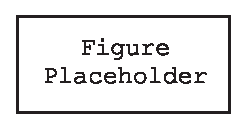
\includegraphics[width=4.6in]{c_cil0/uintrep1.eps}
\caption{Representation Of Unsigned Machine Integers}
\label{fig:ccil0:sroi0:srou0:00}
\end{figure}

\begin{equation}
\label{eq:ccil0:sroi0:srou0:00}
u = \sum_{i=0}^{m-1} u_{[i]} 2^i .
\end{equation}

In general, an $m$-bit unsigned integer can assume the values of 
0 through $2^m - 1$, so that

\begin{equation}
\label{eq:ccil0:sroi0:srou0:01}
u \in \{0, \ldots{} , 2^m - 1 \} .
\end{equation}

Unsigned synthetic long integers are always represented as an array
of unsigned machine integers.  
Consistent with the GMP \cite{bibref:s:gnumultipleprecisionarithmeticlibrary},
we call each element of the array a \emph{limb} and we call the size of
each limb the \emph{limbsize}.  This usage is very close to what Knuth
calls the \emph{word}size $w$ in the excerpt presented in 
Section \ref{ccil0:sppm0:smas0}.

Microcontroller processors are more likely than more powerful processors to have
a non-orthogonal instruction set, and so the limbsize may not be consistent between
operations in an arithmetic library.
With some processors, the appropriate limbsize may vary depending on the operation being
performed.  
For example, a microcontroller processor may be able to add two 16-bit integers to
obtain a 16-bit result plus a carry, but only be able to multiply two 8-bit integers to 
obtain a 16-bit result (thus, the appropriate limbsize for addition may be 
16 bits while the appropriate limbsize for multiplication may be 8 bits).
In such cases, it is usually most efficient to add using 16-bit limbs but
multiply using 8-bit limbs.  Adding using 8-bit limbs on a machine which will
support 16-bit additions is not normally a good design decision---even if the 
machine supports an 8-bit addition instruction which is faster than the 16-bit addition
instruction, $m/2$ 16-bit additions will nearly always be faster than 
$m$ 8-bit additions.  Using different limbsizes within the same arithmetic library
may require some consideration of alignment and 
endian issues, but these are implementation details
which are easily solved.

We view a synthetic long unsigned integer as an array of limbs (machine integers)
of some size, and we agree that we will not address the array in any other way than
by loading and storing limbs of this size.\footnote{Well \ldots{} not quite.
In software for large computers (personal computers and workstations) with an
orthogonal instruction set, we may be able to adhere to this rule.  However,
with microcontrollers, arithmetic libraries which are optimized
may break this rule.}  In particular, because
computers may be ``big-endian'' or ``little-endian'', loading and storing 
smaller units than limbs may lead in
a worst case to software defects or in a best case to non-portable code.

Assume that $w$ is the number of bits in a limb.
Notationally, we denote an unsigned
synthetic long integer as an array of $m$ limbs
$u_{m-1}$ through $u_0$, each containing $w$ bits,
with $u_0$ the least significant machine integer.  
We may also define $b=2^w$ (consistent with Knuth's
notation).
The value of
such a synthetic long machine integer is

\begin{equation}
\label{eq:ccil0:sroi0:srou0:02}
u = \sum_{i=0}^{m-1} u_{i} 2^{wi} 
=
\sum_{i=0}^{m-1} u_{i} b^i.
\end{equation}

As an alternative, we may write the value as the sum of the bit-values,

\begin{equation}
\label{eq:ccil0:sroi0:srou0:03}
u = \sum_{i=0}^{wm-1} u_{[i]} 2^{i} .
\end{equation}

Naturally, the range of such a synthetic long integer is

\begin{equation}
\label{eq:ccil0:sroi0:srou0:04}
u \in \{0, \ldots{} , 2^{wm} - 1 \} .
\end{equation}

In storing an unsigned synthetic long machine integer, the most natural way
to order the array of limbs depends on whether dynamic memory allocation is
used by the arithmetic library.  In microcontroller work, where arithmetic
library subroutines typically operate on fixed-size operands and produce
fixed-size results, storing 
limbs most significant limb first (i.e. in `C', so that element \texttt{[0]}
of the array of limbs contains the most significant limb) may be natural
and convenient.  However, this ordering would lead to computational waste in a library such
as the GMP \cite{bibref:s:gnumultipleprecisionarithmeticlibrary} where integers
may grow arbitrarily large and the library may need to reallocate long synthetic
integers to contain more limbs, as each reallocation would need to be followed
by a memory copy to align the integer's existing limbs to the end of the array.
For libraries such as the GMP, it is more practical to store limbs 
least-significant limb first, as it eliminates the need to copy memory 
when reallocations are done.



%%%%%%%%%%%%%%%%%%%%%%%%%%%%%%%%%%%%%%%%%%%%%%%%%%%%%%%%%%%%%%%%%%%%%%%%%%
%%%%%%%%%%%%%%%%%%%%%%%%%%%%%%%%%%%%%%%%%%%%%%%%%%%%%%%%%%%%%%%%%%%%%%%%%%
%%%%%%%%%%%%%%%%%%%%%%%%%%%%%%%%%%%%%%%%%%%%%%%%%%%%%%%%%%%%%%%%%%%%%%%%%%
\subsection{Representation Of Signed Integers}
%Subsection Tag: ROS0
\label{ccil0:sroi0:sros0}

Signed machine integers are always represented in two's complement form on modern
processors.  This representation is universal because of the digital logic 
conveniences---the same addition and subtraction mappings which are correct 
for unsigned machine integers are also correct for signed machine integers, 
although the criteria for overflow and comparison are
different.

Most readers are familiar with two's complement representation, so we will not
belabor it.  However, we will present essential properties.
When two's complement representation is used in an $m$-bit machine integer $u$:

\begin{enumerate}
\item All bit patterns with $u_{[m-1]} = 0$ represent non-negative integers, and 
      represent the same integer as if the representation were unsigned.
\item All bit patterns with $u_{[m-1]} = 1$ represent negative numbers; specifically
      $u_{[m-2:0]} - 2^{m-1}$; i.e.

      \begin{equation}
      \label{eq:ccil0:sroi0:sros0:00}
      u = - u_{[m-1]} 2^{m-1} + \sum_{i=0}^{m-2} u_{[i]} 2^i .
      \end{equation}

\item $u \in \{-2^{m-1}, \ldots{}, 2^{m-1}-1 \}$.
\item All bit patterns represent a unique integer.
\item For any integer except $-2^{m-1}$, 
      negation can be performed by forming the one's complement (complementing
      every bit), then adding one.  To see why this is true algebraically, note that

\end{enumerate}


However, let us observe that the value of an
$m$-bit two's complement
machine integer is


In general, an $m$-bit signed machine integer can assume the values of 
$-2^{m-1}$ through $2^{m-1} - 1$, so that

\begin{equation}
\label{eq:ccil0:sroi0:sros0:01}
u \in \{-2^{m-1}, \ldots{} , 2^{m-1} - 1 \} .
\end{equation}

There are [at least] two different representations of signed 
multiple-precision integers:

\begin{itemize}
\item Two's complement representation.
\item Sign-magnitude representation.
\end{itemize}

There are two different representations commonly used 
for signed multiple-precision integers because two's complement
representation is not ideal for multiplication and division, although
it is ideal for addition and subtraction.  For multiple-precision
integer arithmetic, sign-magnitude representation is more common.

In two's complement representation of multiple-precision integers,
the representation is the same as suggested by 
(\ref{eq:ccil0:sroi0:sros0:00}), except
more bits are involved.  For a two's complement representation
of a number consisting of $n$ machine integers with $W$ bits per
machine integer,

\begin{equation}
\label{eq:ccil0:sroi0:sros0:02}
u = - u_{B(Wn-1)} 2^{Wn-1} + \sum_{i=0}^{Wn-2} u_{B(i)} 2^i .
\end{equation}

Because we would like to know how to compare signed multiple-precision
integers in two's complement representation, we can gain some
insight into the representation by rewriting 
(\ref{eq:ccil0:sroi0:sros0:02}) in terms of machine integers:

\begin{equation}
\label{eq:ccil0:sroi0:sros0:03}
u = - u_{B(Wn-1)} 2^{Wn-1} 
+ 
\sum_{i=W(m-1)}^{Wn-2} u_{B(i)} 2^i 
+
\sum_{i=0}^{m-2} u_{i} 2^{Wi} .
\end{equation}

(\ref{eq:ccil0:sroi0:sros0:03}) gives some insight into the
relative values of multiple-precision signed two's complement
integers with respect to the values of the machine integers
that comprise them.  We discuss this further in
Section \ref{ccil0:scsi0}.

In sign-magnitude representation of multiple-precision signed two's
complement integers, an integer $u$ is represented as a sign
bit (usually a value of one indicates negativity), and a magnitude, 
which is $|u|$.  Unlike two's complement representation,
sign-magnitude representation, has two representations of zero---a positive
one and a negative one.  Either a canonical form for zero should be
adopted, or both values should be treated identically.

Assuming that the sign bit is stored in the most significant bit position,
it is easy to deduce that the value of a multiple-precision
signed two's complement integer in sign-magnitude representation is

\begin{equation}
\label{eq:ccil0:sros0:srou0:04}
u = (-1)^{u_{B(m-1)}} \sum_{i=0}^{m-2} u_{B(i)} 2^i .
\end{equation}

Sign-magnitude representation is especially convenient because
it allows machine instructions which accept unsigned operands to be used
to make calculations involving signed integers.



%%%%%%%%%%%%%%%%%%%%%%%%%%%%%%%%%%%%%%%%%%%%%%%%%%%%%%%%%%%%%%%%%%%%%%%%%%
%%%%%%%%%%%%%%%%%%%%%%%%%%%%%%%%%%%%%%%%%%%%%%%%%%%%%%%%%%%%%%%%%%%%%%%%%%
%%%%%%%%%%%%%%%%%%%%%%%%%%%%%%%%%%%%%%%%%%%%%%%%%%%%%%%%%%%%%%%%%%%%%%%%%%
\section{Characteristics Of Practical Processors}
%Section tag: CPP
\label{ccil0:scpp0}

Before discussing specific algorithms, it is necessary to 
discuss the construction of practical processors---how such a processor
manipulates machine integers.  We accept as a typical processor the
TMS-370C8, an 8-bit microcontroller manufactured by 
Texas Instruments.

\begin{figure}
\centering
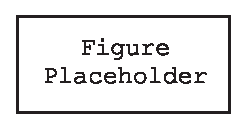
\includegraphics[width=4.6in]{c_cil0/t370flag.eps}
\caption{Texas Instruments TMS-370C8 Flags}
\label{fig:ccil0:scpp0:00}
\end{figure}

\begin{figure}
\centering
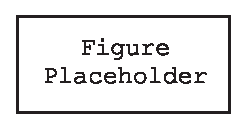
\includegraphics[width=4.6in]{c_cil0/t370cjmp.eps}
\caption{Texas Instruments TMS-370C8 Conditional Jump Instructions}
\label{fig:ccil0:scpp0:01}
\end{figure}

A typical microcontroller allows operations on machine integers
in the following steps:

\begin{itemize}
\item A machine instruction is performed on one or two machine 
      integer operands (for example:  addition, subtraction, 
      multiplication, division, increment, decrement, complement,
      negation, or comparison).  This machine instruction may
      produce a result, and usually sets a number of condition flags that
      reflect the nature and validity of the result (Is it zero?
      Is it negative?  Did the result overflow?).  As an
      example, the condition
      flags of the TMS-370C8 are shown in Figure \ref{fig:ccil0:scpp0:00}.
      .
\item A conditional branch instruction is used to branch conditionally
      based on the state of the condition flags.  The definition of
      the condition flags and the way in which the conditional
      branch instruction utilizes them is designed to provide a
      way to treat both unsigned and signed machine integers.
      As an example, the way in which the conditional
      jump instructions of the TMS-370C8 use the flags
      is shown in Figure \ref{fig:ccil0:scpp0:01}.
\end{itemize}

It is not too often necessary to understand in detail
the Boolean relationships that govern how machine integers are
added, subtracted, and compared; and how signed comparisons differ
from unsigned comparisons.  In most cases, it is adequate to
rely on the design of the microcontroller.  However, we do present
rudimentary observations in this section.



%%%%%%%%%%%%%%%%%%%%%%%%%%%%%%%%%%%%%%%%%%%%%%%%%%%%%%%%%%%%%%%%%%%%%%%%%%
%%%%%%%%%%%%%%%%%%%%%%%%%%%%%%%%%%%%%%%%%%%%%%%%%%%%%%%%%%%%%%%%%%%%%%%%%%
%%%%%%%%%%%%%%%%%%%%%%%%%%%%%%%%%%%%%%%%%%%%%%%%%%%%%%%%%%%%%%%%%%%%%%%%%%
\section{Comparison Of Integers}


%%%%%%%%%%%%%%%%%%%%%%%%%%%%%%%%%%%%%%%%%%%%%%%%%%%%%%%%%%%%%%%%%%%%%%%%%%
%%%%%%%%%%%%%%%%%%%%%%%%%%%%%%%%%%%%%%%%%%%%%%%%%%%%%%%%%%%%%%%%%%%%%%%%%%
%%%%%%%%%%%%%%%%%%%%%%%%%%%%%%%%%%%%%%%%%%%%%%%%%%%%%%%%%%%%%%%%%%%%%%%%%%
\subsection{Comparison Of Unsigned Integers}


%%%%%%%%%%%%%%%%%%%%%%%%%%%%%%%%%%%%%%%%%%%%%%%%%%%%%%%%%%%%%%%%%%%%%%%%%%
%%%%%%%%%%%%%%%%%%%%%%%%%%%%%%%%%%%%%%%%%%%%%%%%%%%%%%%%%%%%%%%%%%%%%%%%%%
%%%%%%%%%%%%%%%%%%%%%%%%%%%%%%%%%%%%%%%%%%%%%%%%%%%%%%%%%%%%%%%%%%%%%%%%%%
\subsection{Comparison Of Signed Integers}
%Section Tag: CSI0
\label{ccil0:scsi0}


%%%%%%%%%%%%%%%%%%%%%%%%%%%%%%%%%%%%%%%%%%%%%%%%%%%%%%%%%%%%%%%%%%%%%%%%%%
%%%%%%%%%%%%%%%%%%%%%%%%%%%%%%%%%%%%%%%%%%%%%%%%%%%%%%%%%%%%%%%%%%%%%%%%%%
%%%%%%%%%%%%%%%%%%%%%%%%%%%%%%%%%%%%%%%%%%%%%%%%%%%%%%%%%%%%%%%%%%%%%%%%%%
\section{Integer Addition}
%Section tag: IAD0
\label{ccil0:siad0}

Addition of two $m$-bit integers is a combinational function---that is,
the inputs uniquely determine the output.  Addition of binary 
numbers is performed 


%%%%%%%%%%%%%%%%%%%%%%%%%%%%%%%%%%%%%%%%%%%%%%%%%%%%%%%%%%%%%%%%%%%%%%%%%%
%%%%%%%%%%%%%%%%%%%%%%%%%%%%%%%%%%%%%%%%%%%%%%%%%%%%%%%%%%%%%%%%%%%%%%%%%%
%%%%%%%%%%%%%%%%%%%%%%%%%%%%%%%%%%%%%%%%%%%%%%%%%%%%%%%%%%%%%%%%%%%%%%%%%%
\subsection{Hardware Implementation Of Addition}


%%%%%%%%%%%%%%%%%%%%%%%%%%%%%%%%%%%%%%%%%%%%%%%%%%%%%%%%%%%%%%%%%%%%%%%%%%
%%%%%%%%%%%%%%%%%%%%%%%%%%%%%%%%%%%%%%%%%%%%%%%%%%%%%%%%%%%%%%%%%%%%%%%%%%
%%%%%%%%%%%%%%%%%%%%%%%%%%%%%%%%%%%%%%%%%%%%%%%%%%%%%%%%%%%%%%%%%%%%%%%%%%
\subsection{Addition Of Unsigned Operands}


%%%%%%%%%%%%%%%%%%%%%%%%%%%%%%%%%%%%%%%%%%%%%%%%%%%%%%%%%%%%%%%%%%%%%%%%%%
%%%%%%%%%%%%%%%%%%%%%%%%%%%%%%%%%%%%%%%%%%%%%%%%%%%%%%%%%%%%%%%%%%%%%%%%%%
%%%%%%%%%%%%%%%%%%%%%%%%%%%%%%%%%%%%%%%%%%%%%%%%%%%%%%%%%%%%%%%%%%%%%%%%%%
\subsection{Addition Of Signed Operands}


%%%%%%%%%%%%%%%%%%%%%%%%%%%%%%%%%%%%%%%%%%%%%%%%%%%%%%%%%%%%%%%%%%%%%%%%%%
%%%%%%%%%%%%%%%%%%%%%%%%%%%%%%%%%%%%%%%%%%%%%%%%%%%%%%%%%%%%%%%%%%%%%%%%%%
%%%%%%%%%%%%%%%%%%%%%%%%%%%%%%%%%%%%%%%%%%%%%%%%%%%%%%%%%%%%%%%%%%%%%%%%%%
\section {Integer Subtraction}


%%%%%%%%%%%%%%%%%%%%%%%%%%%%%%%%%%%%%%%%%%%%%%%%%%%%%%%%%%%%%%%%%%%%%%%%%%
%%%%%%%%%%%%%%%%%%%%%%%%%%%%%%%%%%%%%%%%%%%%%%%%%%%%%%%%%%%%%%%%%%%%%%%%%%
%%%%%%%%%%%%%%%%%%%%%%%%%%%%%%%%%%%%%%%%%%%%%%%%%%%%%%%%%%%%%%%%%%%%%%%%%%
\subsection{Hardware Implementation Of Subtraction}


%%%%%%%%%%%%%%%%%%%%%%%%%%%%%%%%%%%%%%%%%%%%%%%%%%%%%%%%%%%%%%%%%%%%%%%%%%
%%%%%%%%%%%%%%%%%%%%%%%%%%%%%%%%%%%%%%%%%%%%%%%%%%%%%%%%%%%%%%%%%%%%%%%%%%
%%%%%%%%%%%%%%%%%%%%%%%%%%%%%%%%%%%%%%%%%%%%%%%%%%%%%%%%%%%%%%%%%%%%%%%%%%
\subsection{Subtraction Of Unsigned Operands}


%%%%%%%%%%%%%%%%%%%%%%%%%%%%%%%%%%%%%%%%%%%%%%%%%%%%%%%%%%%%%%%%%%%%%%%%%%
%%%%%%%%%%%%%%%%%%%%%%%%%%%%%%%%%%%%%%%%%%%%%%%%%%%%%%%%%%%%%%%%%%%%%%%%%%
%%%%%%%%%%%%%%%%%%%%%%%%%%%%%%%%%%%%%%%%%%%%%%%%%%%%%%%%%%%%%%%%%%%%%%%%%%
\subsection{Subtraction Of Signed Operands}



%%%%%%%%%%%%%%%%%%%%%%%%%%%%%%%%%%%%%%%%%%%%%%%%%%%%%%%%%%%%%%%%%%%%%%%%%%
%%%%%%%%%%%%%%%%%%%%%%%%%%%%%%%%%%%%%%%%%%%%%%%%%%%%%%%%%%%%%%%%%%%%%%%%%%
%%%%%%%%%%%%%%%%%%%%%%%%%%%%%%%%%%%%%%%%%%%%%%%%%%%%%%%%%%%%%%%%%%%%%%%%%%
\section{Integer Multiplication}


%%%%%%%%%%%%%%%%%%%%%%%%%%%%%%%%%%%%%%%%%%%%%%%%%%%%%%%%%%%%%%%%%%%%%%%%%%
%%%%%%%%%%%%%%%%%%%%%%%%%%%%%%%%%%%%%%%%%%%%%%%%%%%%%%%%%%%%%%%%%%%%%%%%%%
%%%%%%%%%%%%%%%%%%%%%%%%%%%%%%%%%%%%%%%%%%%%%%%%%%%%%%%%%%%%%%%%%%%%%%%%%%
\subsection{Hardware Implementation Of Multiplication}


%%%%%%%%%%%%%%%%%%%%%%%%%%%%%%%%%%%%%%%%%%%%%%%%%%%%%%%%%%%%%%%%%%%%%%%%%%
%%%%%%%%%%%%%%%%%%%%%%%%%%%%%%%%%%%%%%%%%%%%%%%%%%%%%%%%%%%%%%%%%%%%%%%%%%
%%%%%%%%%%%%%%%%%%%%%%%%%%%%%%%%%%%%%%%%%%%%%%%%%%%%%%%%%%%%%%%%%%%%%%%%%%
\subsection{Multiplication Of Unsigned Operands}


%%%%%%%%%%%%%%%%%%%%%%%%%%%%%%%%%%%%%%%%%%%%%%%%%%%%%%%%%%%%%%%%%%%%%%%%%%
%%%%%%%%%%%%%%%%%%%%%%%%%%%%%%%%%%%%%%%%%%%%%%%%%%%%%%%%%%%%%%%%%%%%%%%%%%
%%%%%%%%%%%%%%%%%%%%%%%%%%%%%%%%%%%%%%%%%%%%%%%%%%%%%%%%%%%%%%%%%%%%%%%%%%
\subsection{Multiplication Of Signed Operands}



%%%%%%%%%%%%%%%%%%%%%%%%%%%%%%%%%%%%%%%%%%%%%%%%%%%%%%%%%%%%%%%%%%%%%%%%%%
%%%%%%%%%%%%%%%%%%%%%%%%%%%%%%%%%%%%%%%%%%%%%%%%%%%%%%%%%%%%%%%%%%%%%%%%%%
%%%%%%%%%%%%%%%%%%%%%%%%%%%%%%%%%%%%%%%%%%%%%%%%%%%%%%%%%%%%%%%%%%%%%%%%%%
\section{Integer Division}
\label{ccil0:sidv0}

\index{division}\index{integer division}In this section,
we discuss the best known methods of dividing integers using
typical microcontroller instruction sets.  In general, given
two arbitrary integers $p$ and $q$, we are interested in determining
their quotient $q=\lfloor{}p/q\rfloor$ and remainder
$r=p\bmod{}q$ as economically as possible.


%%%%%%%%%%%%%%%%%%%%%%%%%%%%%%%%%%%%%%%%%%%%%%%%%%%%%%%%%%%%%%%%%%%%%%%%%%
%%%%%%%%%%%%%%%%%%%%%%%%%%%%%%%%%%%%%%%%%%%%%%%%%%%%%%%%%%%%%%%%%%%%%%%%%%
%%%%%%%%%%%%%%%%%%%%%%%%%%%%%%%%%%%%%%%%%%%%%%%%%%%%%%%%%%%%%%%%%%%%%%%%%%
\subsection{Hardware Implementation Of Division}


%%%%%%%%%%%%%%%%%%%%%%%%%%%%%%%%%%%%%%%%%%%%%%%%%%%%%%%%%%%%%%%%%%%%%%%%%%
%%%%%%%%%%%%%%%%%%%%%%%%%%%%%%%%%%%%%%%%%%%%%%%%%%%%%%%%%%%%%%%%%%%%%%%%%%
%%%%%%%%%%%%%%%%%%%%%%%%%%%%%%%%%%%%%%%%%%%%%%%%%%%%%%%%%%%%%%%%%%%%%%%%%%
\subsection{General Unsigned Division Without A Machine Division Instruction}
\label{ccil0:sidv0:sgdn0}


%%%%%%%%%%%%%%%%%%%%%%%%%%%%%%%%%%%%%%%%%%%%%%%%%%%%%%%%%%%%%%%%%%%%%%%%%%
%%%%%%%%%%%%%%%%%%%%%%%%%%%%%%%%%%%%%%%%%%%%%%%%%%%%%%%%%%%%%%%%%%%%%%%%%%
%%%%%%%%%%%%%%%%%%%%%%%%%%%%%%%%%%%%%%%%%%%%%%%%%%%%%%%%%%%%%%%%%%%%%%%%%%
\subsection{General Unsigned Division With A Machine Division Instruction}
\label{ccil0:sidv0:sgdu0}

As mentioned many places in this work, efficiency in microcontroller software
involves phrasing computational problems in a way which makes good use of
the machine instruction set.  In Section \ref{ccil0:sidv0:sgdn0} we discussed
the classic shift-compare-subtract algorithm for division.  This algorithm
is far from efficient.  A reasonable question to ask is whether we can
leverage ``small'' division capability (provided by the machine instruction set)
to accomplish ``large'' divisions (those which we require in practice).
It ends up that this is possible:  the technique involved is effectively
to use machine division instructions to estimate the highest-order bits of 
the quotient based on the highest-order bits of the dividend and divisor.

Knuth's discussion of division 
algorithms \cite[pp. 270-275]{bibref:b:knuthclassic2ndedvol2} is the
basis for most of the material in this subsection.  However, Knuth has
a gift for terseness that is sometimes a curse for the reader, and so
we take more time than Knuth to explain certain results.

First, as a starting point, we present \emph{Algorithm D} from
Knuth \cite[pp. 272-273]{bibref:b:knuthclassic2ndedvol2}.  Then,
we justify the algorithm and explain why it is valid.  Finally,
we supply implementation advice for microcontroller instruction sets.

\begin{vworkalgorithmstatementpar}{Arbitrary Unsigned Division Using 
Machine Unsigned Division Instructions}
\label{alg:ccil0:sidv0:sgdu0:01}
(From Knuth \cite[pp. 272-273]{bibref:b:knuthclassic2ndedvol2})
Given nonnegative integers $u=(u_{m+n-1} \ldots{} u_1 u_0)_b$
and $v=(v_{n-1} \ldots{} v_1 v_0)_b$, where
$v_{n-1} \neq 0$ and $n > 1$, we form the radix-$b$ quotient
$\lfloor{}u/v\rfloor{} = (q_m q_{m-1} \ldots{} q_0)_b$ and
the remainder $u \bmod v = (r_{n-1} \ldots{} r_1 r_0)_b$.  When
$n=1$, the simpler algorithm of 
Subsection \ref{ccil0:sidv0:sldm0}
should be used. 

\begin{algblvl0}
\item \label{enumstep:alg:ccil0:sidv0:sgdu0:01:01}
      [Normalize.] Set $d \gets \lfloor{}b/(v_{n-1} + 1)\rfloor$.
      Then set $(u_{m+n} u_{m+n-1} \ldots{} u_1 u_0)_b$ equal to 
      $(u_{m+n-1} \ldots{} u_1 u_0)_b$ times $d$; similarly,
      set $(v_{n-1} \ldots{} v_1 v_0)_b$ equal to 
      $(v_{n-1} \ldots{} v_1 v_0)_b$ times $d$.  (Notice the introduction
      of a new digit position $u_{m+n}$ at the left of
      $u_{m+n-1}$; if $d=1$, all we need to do in this step is set
      $u_{m+n} \gets 0$.  On a binary computer it may be preferable
      to choose $d$ to be a power of 2 instead of using the value
      suggested here; any value of $d$ that results in
      $v_{n-1} \geq \lfloor{}b/2\rfloor$ will suffice.  See also
      exercise 37.)
\item \label{enumstep:alg:ccil0:sidv0:sgdu0:01:02}
      [Initialize $j$.]  Set $j \gets m$.  (The loop on $j$,
      steps 
      \ref{enumstep:alg:ccil0:sidv0:sgdu0:01:03} 
      through 
      \ref{enumstep:alg:ccil0:sidv0:sgdu0:01:07}, 
      will be essentially a division of 
      $(u_{j+n} \ldots{} u_{j+1} u_j)_b$ by $(v_{n-1} \ldots{} v_1 v_0)_b$ to
      get a single quotient digit $q_j$; see Figure \ref{fig:alg:ccil0:sidv0:sgdu0:01:01}.)

\begin{figure}
\centering
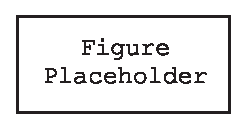
\includegraphics[width=4.6in]{c_cil0/kdfc01.eps}
\caption{Flowchart For Algorithm \ref{alg:ccil0:sidv0:sgdu0:01} (From \cite[p. 273]{bibref:b:knuthclassic2ndedvol2})}
\label{fig:alg:ccil0:sidv0:sgdu0:01:01}
\end{figure}

\item \label{enumstep:alg:ccil0:sidv0:sgdu0:01:03}
      [Calculate $\hat{q}$.]  Set
      $\hat{q} \gets \lfloor{}u_{j+n}b + u_{j+n-1})/v_{n-1}\rfloor$ and
      let $\hat{r}$ be the remainder, $(u_{j+n}b + u_{j+n-1}) \bmod v_{n-1}$.
      Now test if $\hat{q} = b$ or $\hat{q} v_{n-2} > b\hat{r} + u_{j+n-2}$;
      if so, decrease $\hat{q}$ by 1, increase $\hat{r}$ by $v_{n-1}$, and repeat
      this test if $\hat{r} < b$.  (The test of $v_{n-2}$ determines at high
      speed most of the cases in which the trial value $\hat{q}$ is one too large,
      and it eliminates \emph{all} cases where $\hat{q}$ is two too large;
      see exercises 19, 20, 21.)
\item \label{enumstep:alg:ccil0:sidv0:sgdu0:01:04}
      [Multiply and subtract.]  Replace $(u_{j+n} u_{j+n-1} \ldots{} u_j)_b$ by

      \begin{equation}
      \nonumber
      (u_{j+n} u_{j+n-1} \ldots{} u_j)_b - \hat{q} (0 v_{n-1} \ldots{} v_1 v_0)_b. 
      \end{equation}

      This computation consists of a simple multiplication by a one-place number,
      combined with a subtraction.  The digits $(u_{j+n}, u_{j+n-1}, \ldots{}, u_j)$
      should be kept positive; if the result of this step is actually negative, 
      $(u_{j+n} u_{j+n-1} \ldots{} u_j)_b$ should be left as the true
      value plus $b^{n+1}$, namely as the $b$'s complement of the true value, and 
      a ``borrow'' to the left should be remembered.
\item \label{enumstep:alg:ccil0:sidv0:sgdu0:01:05}
      [Test remainder.]  Set $q_j \gets \hat{q}$.  If the result of step 
      \ref{enumstep:alg:ccil0:sidv0:sgdu0:01:04} was negative, go to
      step \ref{enumstep:alg:ccil0:sidv0:sgdu0:01:06}; otherwise go on to
      step \ref{enumstep:alg:ccil0:sidv0:sgdu0:01:07}.
\item \label{enumstep:alg:ccil0:sidv0:sgdu0:01:06}
      [Add back.]  (The probability that this step is necessary is very small, on the 
      order of only $2/b$, as shown in exercise 21; test data to activate this step
      should therefore be specifically contrived when debugging.)  Decrease 
      $q_j$ by 1, and add $(0 v_{n-1} \ldots v_1 v_0)_b$ to
      $(u_{j+n} u_{j+n-1} \ldots{} u_{j+1} u_j)_b$.  (A carry will occur to the left of
      $u_{j+n}$, and it should be ignored since it cancels with the borrow that
      occured in step \ref{enumstep:alg:ccil0:sidv0:sgdu0:01:04}.) 
\item \label{enumstep:alg:ccil0:sidv0:sgdu0:01:07}
      [Loop on $j$.]  Decrease $j$ by one.  Now if $j \geq 0$, go back to step
      \ref{enumstep:alg:ccil0:sidv0:sgdu0:01:03}.
\item \label{enumstep:alg:ccil0:sidv0:sgdu0:01:08}
      [Unnormalize.]  Now $(q_m \ldots{} q_1 q_0)_b$ is the desired quotient, and
      the desired remainder may be obtained by dividing 
      $(u_{n-1} \ldots{} u_1 u_0)_b$ by $d$.
\end{algblvl0}
\end{vworkalgorithmstatementpar}
\vworkalgorithmfooter{}

The general idea of Algorithm \ref{alg:ccil0:sidv0:sgdu0:01} is that 
digits (machine words) of the quotient $q$ can be successively estimated 
based on the first digits of the dividend and divisor.  Knuth
\cite[p. 271]{bibref:b:knuthclassic2ndedvol2} explores the properties of
the digit estimate 

\begin{equation}
\label{eq:ccil0:sidv0:sgdu0:01}
\hat{q} = \min \left( {\left\lfloor{\frac{u_n b + u_{n-1}}{v_{n-1}}}\right\rfloor, b-1} \right).
\end{equation}

The first point to make about an estimate in the form of 
(\ref{eq:ccil0:sidv0:sgdu0:01}) is that it can only be accomplished
efficiently if the machine-native division instruction supports
overflow detection, since it is possible that
$(u_n b + u_{n-1})/v_{n-1} \geq b$, even if 
$u/v < b$, as is shown by the following example.

\begin{vworkexamplestatement}
\label{ex:ccil0:sidv0:sgdu0:01:01}
Assume that we wish to apply the estimate of $\hat{q}$ provided by 
(\ref{eq:ccil0:sidv0:sgdu0:01})
to $u=16,776,704$ and $v=65,535$.  Demonstrate that a machine division
overflow will occur when estimating the first digit, assuming a processor
that can divide a 16-bit dividend by an 8-bit divisor to produce an 8-bit
quotient.
\end{vworkexamplestatement}
\begin{vworkexampleparsection}{Solution}
Note that according to Knuth's intention, the word size on such a machine
is 8 bits.  Thus, $b=256$.  Note that $u/v = 255 + 255/256 < b = 256$, as
required by Knuth's precondition.  However, although $u/v < b$, 
$u = [255 \; 254 \; 0] [256^2 \; 256 \; 1]^T = [u_2 u_1 u_0] [b^2 b^1 b^0]^T$ and 
$v = [255 \; 255] [256 \; 1]^T = [v_1 v_0] [b^1 b^0]^T$, so that calculating
an estimate $\hat{q}$ as required by (\ref{eq:ccil0:sidv0:sgdu0:01}),
$(u_n b + u_{n-1})/v_{n-1} = 65,534/255 = 256 + 254/255 \geq b$, is a division
overflow for a single machine division instruction.  Thus, it follows that 
a machine with division overflow detection can quickly determine that $b-1$ from
(\ref{eq:ccil0:sidv0:sgdu0:01}) is the minimum, whereas a machine without 
division overflow
detection would have to use several additional machine instructions to make
this determination.
\end{vworkexampleparsection}
\vworkexamplefooter{}

The second thing to establish about $\hat{q}$ as defined by 
(\ref{eq:ccil0:sidv0:sgdu0:01}) is how ``good'' of an estimate 
$\hat{q}$ is---how much information, exactly, about $q$ can we
obtain by examining the first two words of $u$ and the first
word of $v$?

We first establish in the following lemma that our estimate of
$q$, $\hat{q}$, can be no less than $q$.

\begin{vworklemmastatementpar}{\mbox{\boldmath$\hat{q} \geq q$}}
\label{lem:ccil0:sidv0:sgdu0:01}
The estimate of $q$ provided by (\ref{eq:ccil0:sidv0:sgdu0:01}),
$\hat{q}$ is always at least as great as the actual value of 
$q$, i.e. $\hat{q} \geq q$.
\end{vworklemmastatementpar}
\begin{vworklemmaproof}
Knowledge of $u_{n}$, $u_{n-1}$, and $v_{n-1}$ necessarily confine
the intervals in which the actual values of $u$ and $v$ may be;
specifically:\footnote{In
(\ref{eq:lem:ccil0:sidv0:sgdu0:01:04})
and 
(\ref{eq:lem:ccil0:sidv0:sgdu0:01:07}),
we use statements of the form ``$x = x$'' as an idiom for
``$x$ is known''.}

\begin{eqnarray}
\label{eq:lem:ccil0:sidv0:sgdu0:01:01}
u & = & \sum_{i=0}^{n} u_i b^i   \\
\label{eq:lem:ccil0:sidv0:sgdu0:01:02}
  & = & u_n b^n + u_{n-1} b^{n-1} + \ldots{} + u_2 b^2 + u_1 b + u_0   \\
\label{eq:lem:ccil0:sidv0:sgdu0:01:03}
  & = & (u_n b + u_{n-1}) b^{n-1} + \ldots{} + u_2 b^2 + u_1 b + u_0
\end{eqnarray}

\begin{eqnarray}
\nonumber & (u_n = u_n \wedge u_{n-1} = u_{n-1}) & \\
\label{eq:lem:ccil0:sidv0:sgdu0:01:04}
& \vworkvimp & \\
\nonumber & (u_n b + u_{n-1}) b^{n-1} \leq u \leq (u_n b + u_{n-1}) b^{n-1} + b^{n-1} - 1 &
\end{eqnarray}

\begin{eqnarray}
\label{eq:lem:ccil0:sidv0:sgdu0:01:05}
v & = & \sum_{i=0}^{n-1} v_i b^i   \\
\label{eq:lem:ccil0:sidv0:sgdu0:01:06}
& = & v_{n-1} b^{n-1} + v_{n-2} b^{n-2} + \ldots{} + v_2 b^2 + v_1 b + v_0 
\end{eqnarray}

\begin{equation}
\label{eq:lem:ccil0:sidv0:sgdu0:01:07}
(v_{n-1} = v_{n-1})
\vworkhimp
v_{n-1} b^{n-1} \leq v \leq v_{n-1} b^{n-1} + b^{n-1} - 1 
\end{equation}

(\ref{eq:lem:ccil0:sidv0:sgdu0:01:04}) and
(\ref{eq:lem:ccil0:sidv0:sgdu0:01:07}) reflect the uncertainties in the 
values of $u$ and $v$ respectively because only the first digit(s) of
$u$ and $v$ are being considered in forming the estimate $\hat{q}$.

By definition, the actual value of $q$ is $\lfloor{}u/v\rfloor$.  For a 
rational function $f(u,v) = u/v$ where $u \in [u_{min}, u_{max}]$ and
$v \in [v_{min}, v_{max}]$, the minimum value of $u/v$ occurs at 
$u_{min}/v_{max}$, and the maximum value of $u/v$ occurs at
$u_{max}/v_{min}$.  We can therefore write that

\begin{equation}
\label{eq:lem:ccil0:sidv0:sgdu0:01:08}
\left\lfloor{\frac{(u_n b + u_{n-1}) b^{n-1}}{v_{n-1} b^{n-1} + b^{n-1} - 1}}\right\rfloor
\leq
q
\leq
\left\lfloor{\frac{(u_n b + u_{n-1}) b^{n-1} + b^{n-1} - 1}{v_{n-1} b^{n-1}}}\right\rfloor .
\end{equation} 

In other words, knowledge of $u_{n}$, $u_{n-1}$, and $v_{n-1}$ confines $q$ to the 
interval indicated in (\ref{eq:lem:ccil0:sidv0:sgdu0:01:08}).  We must prove that,
given a specific $u_{n}$, $u_{n-1}$, and $v_{n-1}$, $\hat{q}$ is at least as large as
the upper bound in (\ref{eq:lem:ccil0:sidv0:sgdu0:01:08}); otherwise we could find a
$q$ such that $q > \hat{q}$.  We can algebraically manipulate the upper bound in 
in (\ref{eq:lem:ccil0:sidv0:sgdu0:01:08}) to yield

\begin{equation}
\label{eq:lem:ccil0:sidv0:sgdu0:01:09}
\left\lfloor{\frac{(u_n b + u_{n-1}) b^{n-1}}{v_{n-1} b^{n-1} + b^{n-1} - 1}}\right\rfloor
\leq
q
\leq
\left\lfloor{\frac{u_n b + u_{n-1} + \frac{b^{n-1}-1}{b^{n-1}}}{v_{n-1}}}\right\rfloor .
\end{equation} 

In (\ref{eq:lem:ccil0:sidv0:sgdu0:01:09}), since $(b^{n-1}-1)/b^{n-1} < 1$ and since
$u_n b + u_{n-1}$ is an integer, we can conclude that
$\lfloor u_n b + u_{n-1} + (b^{n-1}-1)/b^{n-1} \rfloor = \lfloor u_n b + u_{n-1} \rfloor$
and hence that

\begin{equation}
\label{eq:lem:ccil0:sidv0:sgdu0:01:10}
q
\leq
\left\lfloor{\frac{u_n b + u_{n-1} + \frac{b^{n-1}-1}{b^{n-1}}}{v_{n-1}}}\right\rfloor 
=
\left\lfloor{\frac{u_n b + u_{n-1}}{v_{n-1}}}\right\rfloor 
=
\hat{q} .
\end{equation} 

Therefore, $\hat{q} \geq q$.
\end{vworklemmaproof}
\vworklemmafooter{}

Lemma \ref{lem:ccil0:sidv0:sgdu0:01} establishes that 
a digit estimate $\hat{q}$ based on the first digit of the
divisor $v$ can be no less than the actual digit $q$, i.e.
$\hat{q}-q \geq 0$.  However, we must also establish an upper bound
on $\hat{q}-q$.

Intuitively, based on
(\ref{eq:lem:ccil0:sidv0:sgdu0:01:06}), we might guess that
if $v_{n-1}$ is small, the estimate $\hat{q}$ may be quite
poor, as the interval to which the actual value of $v$ is confined
may be quite large.  This fact is the basis for the normalization
step [\ref{enumstep:alg:ccil0:sidv0:sgdu0:01:01}] in Algorithm
\ref{alg:ccil0:sidv0:sgdu0:01}.  We now prove a useful result
for how much $u, v$ must be normalized so that $\hat{q}-q \leq 2$.

\begin{vworklemmastatementpar}{Normalization Requirement So That 
                               \mbox{\boldmath$\hat{q} - q \leq 2$}}
\label{lem:ccil0:sidv0:sgdu0:02}
If $v_{n-1} \geq \lfloor b/2 \rfloor$ and $\hat{q}$ is chosen as
indicated in (\ref{eq:ccil0:sidv0:sgdu0:01}), then 
$0 \leq \hat{q} - q \leq 2$.
\end{vworklemmastatementpar}
\begin{vworklemmaproof}
The lower limit on $\hat{q} - q$ is proved in Lemma \ref{lem:ccil0:sidv0:sgdu0:01}.
We now seek only to prove that $\hat{q} - q \leq 2$.
By definition of $\hat{q}$ and $q$, 

\begin{equation}
\label{eq:lem:ccil0:sidv0:sgdu0:02:01}
\hat{q} - q  =    \left\lfloor {\frac{u_n b + u_{n-1}}{v_{n-1}}} \right\rfloor 
                  - \left\lfloor {\frac{u}{v}} \right\rfloor 
\end{equation}

When only nonnegative integers are involved, 
(\cmtnzeroxrefhyphen\ref{eq:cmtn0:sfcf0:02}) 
supplies an exact expression for the floor of a 
ratio of integers.  Using (\cmtnzeroxrefhyphen\ref{eq:cmtn0:sfcf0:02}),
(\ref{eq:lem:ccil0:sidv0:sgdu0:02:01}) can be decomposed into

\begin{equation}
\label{eq:lem:ccil0:sidv0:sgdu0:02:02}
\hat{q} - q  =    \frac{u_n b + u_{n-1}}{v_{n-1}}
                - \frac{(u_n b + u_{n-1}) \bmod v_{n-1}}{v_{n-1}}
                - \frac{u}{v}
                + \frac{u \bmod v}{v} . 
\end{equation}

\noindent{}Note that (\ref{eq:lem:ccil0:sidv0:sgdu0:02:02}) is an exact 
expression (rather than an
inequality).

Note in (\ref{eq:lem:ccil0:sidv0:sgdu0:02:02}) that
$(u_n b + u_{n-1}) \bmod v_{n-1} \in [0, v_{n-1}-1]$, and that in general
there is no reason to expect it cannot be zero.  Thus, we can assume that
it \emph{is} zero, which will maximize $\hat{q}-q$.  We can thus convert
(\ref{eq:lem:ccil0:sidv0:sgdu0:02:02}) into the inequality

\begin{equation}
\label{eq:lem:ccil0:sidv0:sgdu0:02:03}
\hat{q} - q  \leq \frac{u_n b + u_{n-1}}{v_{n-1}}
                - \frac{u}{v}
                + \frac{u \bmod v}{v} . 
\end{equation}

In (\ref{eq:lem:ccil0:sidv0:sgdu0:02:03}) we can also observe that
$(u \bmod v)/v \in [0, (v-1)/v]$.  If we replace this expression with 
``1'' (which is unattainable, but barely), this will change the relational
operator from ``$\leq$'' to ``$<$'':

\begin{equation}
\label{eq:lem:ccil0:sidv0:sgdu0:02:04}
\hat{q} - q  <    \frac{u_n b + u_{n-1}}{v_{n-1}}
                - \frac{u}{v}
                + 1 . 
\end{equation}

The result we wish to show is that with $v_{n-1} \geq \lfloor b/2 \rfloor$,
$\hat{q}-q \leq 2$.  To simplify the subsequent algebraic manipulations, note in 
(\ref{eq:lem:ccil0:sidv0:sgdu0:02:04}) that

\begin{eqnarray}
\label{eq:lem:ccil0:sidv0:sgdu0:02:05}
          & \hat{q} - q  \leq 2 &  \\    
\nonumber & \vworkvertequiv     &  \\
\label{eq:lem:ccil0:sidv0:sgdu0:02:06}
          & \displaystyle \frac{u_n b + u_{n-1}}{v_{n-1}}
                - \frac{u}{v}
                + 1 \leq 3 &          \\
\nonumber & \vworkvertequiv     &  \\
\label{eq:lem:ccil0:sidv0:sgdu0:02:07}
          & \displaystyle \frac{u_n b + u_{n-1}}{v_{n-1}}
                - \frac{u}{v} \leq 2    &
\end{eqnarray}

(\ref{eq:lem:ccil0:sidv0:sgdu0:02:06}) may be counterintuitive, so
further explanation is offered here.  Since $\hat{q} \in \vworkintset$ and $q \in \vworkintset$,
$\hat{q}-q \in \vworkintset$.  Thus, proving 
(\ref{eq:lem:ccil0:sidv0:sgdu0:02:06}) or
(\ref{eq:lem:ccil0:sidv0:sgdu0:02:07}) proves that
$\hat{q}-q \in \{ \ldots, -1, 0, 1, 2 \}$ (however, by 
Lemma \ref{lem:ccil0:sidv0:sgdu0:01}, $\hat{q}-q \geq 0$, so in fact
what would be proved is that $\hat{q}-q \in \{ 0, 1, 2 \}$).  For 
algebraic simplicity,
we choose to prove (\ref{eq:lem:ccil0:sidv0:sgdu0:02:07}).

First, adjust numerator and denominator of the first term in 
(\ref{eq:lem:ccil0:sidv0:sgdu0:02:07}) by $b^{n-1}$ so that the terms more closely 
resemble $u$ and $v$ in 
(\ref{eq:lem:ccil0:sidv0:sgdu0:01:02}) 
and 
(\ref{eq:lem:ccil0:sidv0:sgdu0:01:06}):

\begin{equation}
\label{eq:lem:ccil0:sidv0:sgdu0:02:08}
\frac{u_n b^n + u_{n-1} b^{n-1}}{v_{n-1} b^{n-1}}
                - \frac{u}{v} \leq 2 .
\end{equation}

For logical implication to be maintained,
we must make the most pessimistic choices and assumptions possible in 
(\ref{eq:lem:ccil0:sidv0:sgdu0:02:08}) in order to maximize the value
of the left side of the inequality.
The first assumption to be made is the error in estimating
$u$ and $v$ based on their most significant digits.  It can be
seen that (\ref{eq:lem:ccil0:sidv0:sgdu0:02:08}) will be maximized if:

\begin{itemize}
\item We assume that $u = u_{n} b^n + u_{n-1} b^{n-1}$ (i.e. that we estimate
      $u$ precisely).
\item We assume that $v = v_{n-1} b^{n-1} + b^{n-1} - 1$ (i.e. that
      we underestimate $v$ by the maximum amount possible).
\item We minimize the value of $v_{n-1} b^{n-1}$.
\end{itemize}

Assuming that $u$ is estimated precisely yields

\begin{equation}
\label{eq:lem:ccil0:sidv0:sgdu0:02:09}
\frac{u}{v_{n-1} b^{n-1}}
                - \frac{u}{v} \leq 2 .
\end{equation}

Assuming that $v$ is underestimated by the maximum amount possible
yields

\begin{equation}
\label{eq:lem:ccil0:sidv0:sgdu0:02:10}
\frac{u}{v - b^{n-1} + 1}
                - \frac{u}{v} \leq 2 .
\end{equation}

Finally, with $b$ and $v$ fixed, $u$ can be maximized by noting that 
$u \leq bv - 1$ (by the problem assumption that the quotient is a single digit).
However, for algebraic simplicity, we make the substitution $u=bv$ (rather than 
$u=bv-1$), since the weaker upper bound is strong enough to prove the 
first result we seek.

\begin{equation}
\label{eq:lem:ccil0:sidv0:sgdu0:02:11}
\frac{bv}{v - b^{n-1} + 1}
                - \frac{bv}{v} \leq 2
\end{equation}

\begin{equation}
\label{eq:lem:ccil0:sidv0:sgdu0:02:12}
\frac{bv}{v - b^{n-1} + 1}
                - b \leq 2
\end{equation}

Solving (\ref{eq:lem:ccil0:sidv0:sgdu0:02:12})
for $v$ yields

\begin{equation}
\label{eq:lem:ccil0:sidv0:sgdu0:02:13}
v \geq \frac{b^n}{2} + b^{n-1} - \frac{1}{b} - 1
\end{equation}

Again using the assumption that $v$ is underestimated by the maximum amount
possible, we may make the substitution that $v = v_{n-1} b^{n-1} + b^{n-1} -1$,
leading to

\begin{equation}
\label{eq:lem:ccil0:sidv0:sgdu0:02:13b}
v_{n-1} \geq \frac{b}{2} - \frac{1}{2 b^{n-2}} .
\end{equation}

There are two cases to consider:  $b$ even and $b$ odd.  If $b$ is even, the
proof is complete, as $\lfloor b/2 \rfloor = b/2$ and the choice of 
$v_{n-1} = \lfloor b/2 \rfloor$ will automatically satisfy
(\ref{eq:lem:ccil0:sidv0:sgdu0:02:13b}).  However, if $b$ is odd, 
$\lfloor b/2 \rfloor = b/2 - 1/2 < b/2 - 1/2b^{n-2}$, violating
(\ref{eq:lem:ccil0:sidv0:sgdu0:02:13b}),
and so we need to
further examine this case.

If $b$ is odd and $v_{n-1} = \lfloor b/2 \rfloor$, then 
$v_{n-1} = b/2 - 1/2$, violating (\ref{eq:lem:ccil0:sidv0:sgdu0:02:13b}).
However, any larger choice of $v_{n-1}$ (such as
$\lfloor b/2 \rfloor + 1$, $\lfloor b/2 \rfloor + 2$, etc.) satisfies
(\ref{eq:lem:ccil0:sidv0:sgdu0:02:13b}); so that it remains only to prove
the $v_{n-1} = \lfloor b/2 \rfloor = b/2 - 1/2$
case.

If $v_{n-1} = \lfloor b/2 \rfloor = b/2 - 1/2$, then

\begin{eqnarray}
\label{eq:lem:ccil0:sidv0:sgdu0:02:14}
v & \in & \left[ 
\left( \frac{b}{2} - \frac{1}{2}\right) b^{n-1},
\left( \frac{b}{2} - \frac{1}{2}\right) b^{n-1} + b^{n-1} - 1
\right] \\
\nonumber & = &
\left[
\frac{b^n}{2} - \frac{b^{n-1}}{2},
\frac{b^n}{2} + \frac{b^{n-1}}{2} -1
\right] .
\end{eqnarray}

Note in this case that the estimation error ($v - v_{n-1}b^{n-1}$) and the
value of $v$ are not independent; and in fact it is this aspect
of the problem that has led to the violation of 
(\ref{eq:lem:ccil0:sidv0:sgdu0:02:13b}) with $b$ odd and 
$v_{n-1} = \lfloor b/2 \rfloor$.

In order to prove the case of $b$ odd and $v = \lfloor b/2 \rfloor = b/2 - 1/2$, 
we must reexamine some simplifying assumptions made earlier in order to obtain
tighter inequalities.  In (\ref{eq:lem:ccil0:sidv0:sgdu0:02:02}), we can no
longer accept the maximum of $(u \bmod v)/v$ as one; instead we construct the 
tighter inequality

\begin{eqnarray}
\label{eq:lem:ccil0:sidv0:sgdu0:02:15}
& \displaystyle \hat{q} - q \leq  \frac{u_n b + u_{n-1}}{v_{n-1}}
                - \frac{u}{v}
                + \frac{u \bmod v}{v} & \\
\nonumber &  \vworkvimp & \\
\label{eq:lem:ccil0:sidv0:sgdu0:02:16}
& \displaystyle \hat{q} - q \leq  \frac{u_n b + u_{n-1}}{v_{n-1}}
                - \frac{u}{v}
                + \frac{v-1}{v} , &
\end{eqnarray}

which leads to

\begin{equation}
\label{eq:lem:ccil0:sidv0:sgdu0:02:17}
\frac{u_n b + u_{n-1}}{v_{n-1}}
                - \frac{u+1}{v}
                < 2 .
\end{equation}

In order to maximize the left-hand side of
(\ref{eq:lem:ccil0:sidv0:sgdu0:02:17}), we assume that we
estimate $u$ exactly so that $u = u_n b^n + u_{n-1} b^{n-1}$,
yielding

\begin{equation}
\label{eq:lem:ccil0:sidv0:sgdu0:02:18}
\frac{u}{v_{n-1} b^{n-1}}
                - \frac{u+1}{v}
                < 2 .
\end{equation}

We also assume that $u$ is the maximum value
possible, $u=bv-1$, leading to

\begin{equation}
\label{eq:lem:ccil0:sidv0:sgdu0:02:19}
\frac{bv-1}{v_{n-1} b^{n-1}}
                - b
                < 2 .
\end{equation}

Finally, we assume that $v$ is the upper limit in
(\ref{eq:lem:ccil0:sidv0:sgdu0:02:14}),
$v=b^n/2 + b^{n-1}/2 - 1$, and substitute the known value of
$v_{n-1}$ for the case being proved, $v_{n-1} = b/2-1/2$, yielding

\begin{equation}
\label{eq:lem:ccil0:sidv0:sgdu0:02:20}
\frac{b \left( \frac{b^n}{2} + \frac{b^{n-1}}{2} - 1 \right) - 1}
{\left( \frac{b}{2} - \frac{1}{2} \right) b^{n-1}}
                - b
                < 2 .
\end{equation}
 
Simplification of (\ref{eq:lem:ccil0:sidv0:sgdu0:02:20})
will establish that it is always true.  This completes the proof.
\end{vworklemmaproof}
\vworklemmafooter{}

Lemmas \ref{lem:ccil0:sidv0:sgdu0:01} and
\ref{lem:ccil0:sidv0:sgdu0:02}, 
standing alone, lead to a good implementation of 
division without any further results.  If it is known that
$0 \leq \hat{q} - q \leq 2$, Algorithm \ref{alg:ccil0:sidv0:sgdu0:01}
can be trivially modified to only calculate
$\hat{q}$ (omitting the additional tests in Step \ref{enumstep:alg:ccil0:sidv0:sgdu0:01:03}), 
and then
to include up to two add-back steps
(duplication of Step \ref{enumstep:alg:ccil0:sidv0:sgdu0:01:06}).  
Although such an algorithm would be 
satisfactory, it has the disadvantage that the add-back steps would
be executed very frequently, slowing the algorithm substantially, especially
for long operands.
We now show that the additional tests in Step \ref{enumstep:alg:ccil0:sidv0:sgdu0:01:03} of 
Algorithm \ref{alg:ccil0:sidv0:sgdu0:01} can eliminate 
altogether the case of $\hat{q}-q = 2$ (Lemma \ref{lem:ccil0:sidv0:sgdu0:03}), and 
can with a probability close to unity eliminate the
case of $\hat{q}-q = 1$ (Lemmas \ref{lem:ccil0:sidv0:sgdu0:04} 
and \ref{lem:ccil0:sidv0:sgdu0:05}).  Together these tests, which are present in 
the statement of Algorithm \ref{alg:ccil0:sidv0:sgdu0:01},
reduce add-back (Step \ref{enumstep:alg:ccil0:sidv0:sgdu0:01:06}) to rare occurrence, and create a more
efficient algorithm than would be possible with the
results of Lemmas \ref{lem:ccil0:sidv0:sgdu0:01} and \ref{lem:ccil0:sidv0:sgdu0:02} alone.

\begin{vworklemmastatementpar}
{\mbox{\boldmath$\hat{q} v_{n-2} \leq b \hat{r} + u_{j+n-2} \vworkhimp 0 \leq \hat{q} - q \leq 1$}}
\label{lem:ccil0:sidv0:sgdu0:03}
If the divisor normalization requirement ($v_{n-1} \geq \lfloor b/2 \rfloor$) as specified in
Step \ref{enumstep:alg:ccil0:sidv0:sgdu0:01:01} of
Algorithm \ref{alg:ccil0:sidv0:sgdu0:01} is met, then

\begin{equation}
\label{eq:lem:ccil0:sidv0:sgdu0:03:01}
\hat{q} v_{n-2} \leq b \hat{r} + u_{j+n-2} \vworkhimp 0 \leq \hat{q} - q \leq 1 .
\end{equation}
\end{vworklemmastatementpar}
\begin{vworklemmaproof}
For reference, note that:

\begin{eqnarray}
\label{eq:lem:ccil0:sidv0:sgdu0:03:02}
u & = & u_{j+n} b^{j+n} + u_{j+n-1} b^{j+n-1} + \ldots{} + u_1 b + u_0 \\
\label{eq:lem:ccil0:sidv0:sgdu0:03:03}
v & = & v_{n-1} b^{n-1} + v_{n-2} b^{n-2} + \ldots{} + v_1 b + v_0
\end{eqnarray}

By definition, we the remainder
$\hat{r}$ has the value
$\hat{r} = u_{j+n} b + u_{j+n-1} - \hat{q} v_{n-1}$.  Substituting this value
into (\ref{eq:lem:ccil0:sidv0:sgdu0:03:01}) produces

\begin{equation}
\label{eq:lem:ccil0:sidv0:sgdu0:03:04}
\hat{q} v_{n-2} \leq b (u_{j+n} b + u_{j+n-1} - \hat{q} v_{n-1}) + u_{j+n-2} ,
\end{equation}

and solving for $\hat{q}$ yields

\begin{equation}
\label{eq:lem:ccil0:sidv0:sgdu0:03:05}
\hat{q} \leq  \frac{u_{j+n} b^2 + u_{j+n-1}b + u_{j+n-2}}{v_{n-1}b + v_{n-2}}.
\end{equation}

It is known from Lemma \ref{lem:ccil0:sidv0:sgdu0:01} that the type of estimate
represented by the floor of the right-hand size of (\ref{eq:lem:ccil0:sidv0:sgdu0:03:05})
can be no less than $q$, leading to

\begin{eqnarray}
\label{eq:lem:ccil0:sidv0:sgdu0:03:06}
& \displaystyle q  \leq  \hat{q}
\leq
\left\lfloor { \frac{u_{j+n} b^2 + u_{j+n-1}b + u_{j+n-2}}{v_{n-1}b + v_{n-2}} } \right\rfloor & \\
\nonumber & \displaystyle \leq  
\frac{u_{j+n} b^2 + u_{j+n-1}b + u_{j+n-2}}{v_{n-1}b + v_{n-2}}. &
\end{eqnarray}

Because $q, \hat{q} \in \vworkintset$, it is only necessary to prove that

\begin{equation}
\label{eq:lem:ccil0:sidv0:sgdu0:03:07}
\frac{u_{j+n} b^2 + u_{j+n-1}b + u_{j+n-2}}{v_{n-1}b + v_{n-2}} -
\left\lfloor \frac{u}{v} \right\rfloor
< 2
\end{equation}

in order to prove that $\hat{q}-q \leq 1$.  Using
(\cmtnzeroxrefhyphen\ref{eq:cmtn0:sfcf0:02}), 
(\ref{eq:lem:ccil0:sidv0:sgdu0:03:07}) can be rewritten as

\begin{equation}
\label{eq:lem:ccil0:sidv0:sgdu0:03:08}
\frac{u_{j+n} b^2 + u_{j+n-1}b + u_{j+n-2}}{v_{n-1}b + v_{n-2}} -
\frac{u}{v} -
\frac{u \bmod v}{v}
< 2 .
\end{equation}

In order for implication to hold, we must make the most pessimistic
assumptions about $u \bmod v$ (those which maximize it).  The maximum value
of $u \bmod v$ is $v-1$, leading to

\begin{equation}
\label{eq:lem:ccil0:sidv0:sgdu0:03:09}
\frac{u_{j+n} b^2 + u_{j+n-1}b + u_{j+n-2}}{v_{n-1}b + v_{n-2}} -
\frac{u + 1}{v}
< 1 .
\end{equation}

In order to maximize the left side of (\ref{}),
we must assume that $u$ is maximized, $v$ is minimized, 


\end{vworklemmaproof}
\vworklemmafooter{}

\begin{vworklemmastatementpar}
{\mbox{\boldmath$\hat{q} v_{n-2} > b \hat{r} + u_{n-2} \vworkhimp q < \hat{q}$}}
\label{lem:ccil0:sidv0:sgdu0:04}
Given $\hat{q} > 0$, an estimate of $q$, and the remainder
based on the estimate, $\hat{r} = u_n b + u_{n-1} - \hat{q} v_{n-1}$,

\begin{equation}
\label{eq:lem:ccil0:sidv0:sgdu0:04:01}
\hat{q} v_{n-2} > b \hat{r} + u_{n-2} \vworkhimp \hat{q} > q .
\end{equation}
\end{vworklemmastatementpar}
\begin{vworklemmaproof}
We make the assumption that $v_{n-1}$ and $v_{n-2}$ are not both 0.
$v_{n-1} > 0$ is guaranteed by
the  normalization of 
$v$ in Algorithm \ref{alg:ccil0:sidv0:sgdu0:01}.

\begin{equation}
\label{eq:lem:ccil0:sidv0:sgdu0:04:02}
\hat{q} v_{n-2} > b \hat{r} + u_{n-2}
\end{equation}

\begin{equation}
\label{eq:lem:ccil0:sidv0:sgdu0:04:03}
\hat{q} v_{n-2} > b (u_n b + u_{n-1} - \hat{q} v_{n-1}) + u_{n-2}
\end{equation}

Solving (\ref{eq:lem:ccil0:sidv0:sgdu0:04:03}) for $\hat{q}$ yields

\begin{equation}
\label{eq:lem:ccil0:sidv0:sgdu0:04:04}
\hat{q} 
>
\frac{u_n b^2 + u_{n-1} b + u_{n-2}}{v_{n-1} b + v_{n-2}}
\geq
\left\lfloor {\frac{u_n b^2 + u_{n-1} b + u_{n-2}}{v_{n-1} b + v_{n-2}}} \right\rfloor
.
\end{equation}

Note that the right-hand term of 
(\ref{eq:lem:ccil0:sidv0:sgdu0:04:04})
is similar in form to the estimate $\hat{q}$ in
Lemma \ref{lem:ccil0:sidv0:sgdu0:01}, where it is proved that
$\hat{q} \geq q$.  It is possible to use identical algebraic technique
as is used in Lemma \ref{lem:ccil0:sidv0:sgdu0:01} in order to prove that

\begin{equation}
\label{eq:lem:ccil0:sidv0:sgdu0:04:05}
\left\lfloor {\frac{u_n b^2 + u_{n-1} b + u_{n-2}}{v_{n-1} b + v_{n-2}}} \right\rfloor
\geq q,
\end{equation}

and it follows that

\begin{equation}
\label{eq:lem:ccil0:sidv0:sgdu0:04:06}
\hat{q} 
>
\frac{u_n b^2 + u_{n-1} b + u_{n-2}}{v_{n-1} b + v_{n-2}}
\geq
\left\lfloor {\frac{u_n b^2 + u_{n-1} b + u_{n-2}}{v_{n-1} b + v_{n-2}}} \right\rfloor
\geq q,
\end{equation}

and thus $\hat{q} > q$.
\end{vworklemmaproof}
\vworklemmafooter{}

\begin{vworklemmastatementpar}
{Add-back occurs with approximate probability \mbox{\boldmath$2/b$}}
\label{lem:ccil0:sidv0:sgdu0:05}
The estimate of $q$ provided by (\ref{eq:ccil0:sidv0:sgdu0:01}),
\end{vworklemmastatementpar}
\begin{vworklemmaproof}
\end{vworklemmaproof}
\vworklemmafooter{}


%%%%%%%%%%%%%%%%%%%%%%%%%%%%%%%%%%%%%%%%%%%%%%%%%%%%%%%%%%%%%%%%%%%%%%%%%%
%%%%%%%%%%%%%%%%%%%%%%%%%%%%%%%%%%%%%%%%%%%%%%%%%%%%%%%%%%%%%%%%%%%%%%%%%%
%%%%%%%%%%%%%%%%%%%%%%%%%%%%%%%%%%%%%%%%%%%%%%%%%%%%%%%%%%%%%%%%%%%%%%%%%%
\subsection{Division Of Signed Operands}


%%%%%%%%%%%%%%%%%%%%%%%%%%%%%%%%%%%%%%%%%%%%%%%%%%%%%%%%%%%%%%%%%%%%%%%%%%
%%%%%%%%%%%%%%%%%%%%%%%%%%%%%%%%%%%%%%%%%%%%%%%%%%%%%%%%%%%%%%%%%%%%%%%%%%
%%%%%%%%%%%%%%%%%%%%%%%%%%%%%%%%%%%%%%%%%%%%%%%%%%%%%%%%%%%%%%%%%%%%%%%%%%
\subsection{Large Dividends With Machine-Native Divisors}
\label{ccil0:sidv0:sldm0}

Division of arbitrary-sized operands (Section \ref{ccil0:sidv0:sgdu0}) is
a costly operation.  In many practical applications, we are able to exploit
data sizes of operands or special relationships between the values of
operands to use the instruction set of the machine more effectively.
In this subsection, we investigate what optimizations we may achieve when:

\begin{itemize}
\item We wish to calculate the quotient and remainder of
      unsigned integers $p$ and $q$:  $p/q$ and 
      $p \bmod{} q$; \emph{and}
\item The machine possesses unsigned division instructions
      which provide both a quotient and a remainder from 
      a division; \emph{and}
\item The bitsize of the divisor $q$ is not larger than can
      be accomodated (as a divisor) by machine division instructions.
\end{itemize}

Processors which possess integer division instructions usually
possess one of two types of instructions:

\begin{itemize}
\item Instructions where the the divisor, quotient and remainder are
      $Q$ bits, but the dividend is $2Q$ bits (we call these
      ``large dividend'' instructions).  For example, an
      instruction which accepts a 16-bit dividend and an
      8-bit divisor to produce an 8-bit quotient and an 8-bit remainder is
      typical.
      With such instructions, overflow is possible, and is always detectable.
      However, in this subsection we never describe algorithms which detect
      overflow---instead, we arrange for data values which cannot generate an
      overflow.
\item Instructions where the dividend, divisor, quotient, and remainder
      are all $Q$ bits (we call these ``small dividend'' instructions).  
      With such instructions, overflow is not possible.
\end{itemize}

We call the bitsize $Q$ a \emph{chunk}.  We use \emph{chunk} rather than
\emph{word} because the chunksize and wordsize in general are not
required to be the same.

For the remainder of this discussion, we assume large dividend 
instructions (the first category above).
The algorithms developed can be implemented on small dividend machines
by halving data sizes so that the divisor fills no more than half
of the available bits.

We assume that we are interested in calculating the integer quotient 
$\lfloor{}p/q\rfloor$ and remainder $p \bmod{} q$ of two unsigned
integers $p$ and $q$, where $p$ is of size $P$ bits and $q$ is
of size $Q$ bits.  For simplicity and without detracting from the
generality of the solution, we assume that $Q \vworkdivides{} P$.

We then seek to calculate

\begin{eqnarray}
\label{eq:ccil0:sidv0:sldm0:001}
\frac{p}{q} & = & \frac{2^{P-Q} p_{[P/Q-1]} + 2^{P-2Q} p_{[P/Q-2]} + \ldots{} + 2^{Q} p_{[1]} + p_{[0]}}{q_{[0]}} \\
\nonumber       & = & \frac{\sum_{i=0}^{P/Q-1} 2^{iQ} p_{[i]}}{q_{[0]}} .
\end{eqnarray}

\noindent{}Using the integer identity

\begin{equation}
\label{eq:ccil0:sidv0:sldm0:002}
\frac{a}{b} = \left\lfloor{\frac{a}{b}}\right\rfloor + \frac{a \bmod b}{b} ,
\end{equation}

\noindent{}we can reform (\ref{eq:ccil0:sidv0:sldm0:001}) into

\begin{eqnarray}
\nonumber
\frac{p}{q} & = &   2^{P-Q} \left\lfloor{\frac{p_{[P/Q-1]}}{q_{[0]}}}\right\rfloor \\
\label{eq:ccil0:sidv0:sldm0:003}
            & + &   2^{P-Q} \frac{p_{[P/Q-1]}\bmod q_{[0]}}{q_{[0]}}
                  + 2^{P-2Q} \frac{p_{[P/Q-2]}}{q_{[0]}}  \\
\nonumber   & + &   \frac{\sum_{i=0}^{P/Q-3} 2^{iQ} p_{[i]}}{q_{[0]}} ,
\end{eqnarray}

\noindent{}which can be polished slightly to yield

\begin{eqnarray}
\nonumber
\frac{p}{q} & = &   2^{P-Q} \left\lfloor{\frac{p_{[P/Q-1]}}{q_{[0]}}}\right\rfloor \\
\label{eq:ccil0:sidv0:sldm0:004}
            & + &   2^{P-2Q} \frac{2^Q (p_{[P/Q-1]}\bmod q_{[0]}) + p_{[P/Q-2]}}{q_{[0]}} \\
\nonumber   & + &   \frac{\sum_{i=0}^{P/Q-3} 2^{iQ} p_{[i]}}{q_{[0]}} .
\end{eqnarray}

Note in (\ref{eq:ccil0:sidv0:sldm0:004}) that the first term, 
$\lfloor{}p_{[P/Q-1]} / q_{[0]}\rfloor$, as well as
a portion of the second term, $p_{[P/Q-1]}\bmod q_{[0]}$, can be 
calculated using a single machine division instruction with
$p_{[P/Q-1]}$ as the dividend and $q_{[0]}$ as the divisor.
Note also that multiplication of an integer by a power of 2
can be achieved by placing the integer correctly within the 
result.  In this regard note that $Q=8$ or $Q=16$ are
the most typical cases, and so the placement can be achieved simply
by selecting the correct memory address.

It is initially unclear whether we can evaluate or reduce the fraction in the 
second term of (\ref{eq:ccil0:sidv0:sldm0:004}),
$[2^Q (p_{[P/Q-1]}\bmod q_{[0]}) + p_{[P/Q-2]}] / q_{[0]}$,
using a single large dividend machine instruction, because
the upper chunk of the dividend is populated with non-zero bits
(specifically, $p_{[P/Q-1]}\bmod q_{[0]}$), and it seems that 
a division overflow may be possible.  However, with some thought,
it is clear that $p_{[P/Q-1]}\bmod q_{[0]} \leq q_{[0]} - 1$ and 
$p_{[P/Q-2]} \leq 2^Q - 1$, thus the largest numerator possible
is $2^Q q_{[0]} - 1$, which, when divided by $q_{[0]}$, will result
in a quotient and remainder of $2^Q - 1$.  Thus, no division overflow
can occur, and the fraction in the  
second term of (\ref{eq:ccil0:sidv0:sldm0:004}) can be evaluated
using a large divisor integer machine instruction.

The fraction in the 
second term of (\ref{eq:ccil0:sidv0:sldm0:004}) can be simplified 
using (\ref{eq:ccil0:sidv0:sldm0:002}) to yield:

\begin{eqnarray}
\nonumber
\frac{p}{q} & = &   2^{P-Q} \left\lfloor{\frac{p_{[P/Q-1]}}{q_{[0]}}}\right\rfloor \\
\label{eq:ccil0:sidv0:sldm0:005}
            & + &   2^{P-2Q} \left\lfloor{\frac{2^Q (p_{[P/Q-1]}\bmod q_{[0]}) + p_{[P/Q-2]}}{q_{[0]}}}\right\rfloor \\
\nonumber   & + &   2^{P-2Q} \frac{(2^Q (p_{[P/Q-1]}\bmod q_{[0]}) + p_{[P/Q-2]}) \bmod q_{[0]}}{q_{[0]}} \\
\nonumber   & + &   \frac{\sum_{i=0}^{P/Q-3} 2^{iQ} p_{[i]}}{q_{[0]}} .
\end{eqnarray}

The process of combining adjacent terms can be continued until all
divisions and modulo operations necessary can be carried out using
long dividend division instructions.  If we envision a 
long-dividend division instruction as a functional block that
accepts a $2Q$-bit dividend and a $Q$-bit divisor to produce a
$Q$-bit quotient and a $Q$-bit remainder
(Figure \ref{fig:ccil0:sidv0:sldm0:00}), then we can draw the
entire division as outlined by (\ref{eq:ccil0:sidv0:sldm0:005})
as shown in Figure \ref{fig:ccil0:sidv0:sldm0:01}.

\begin{figure}
\centering
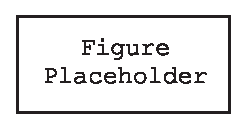
\includegraphics[width=4.6in]{c_cil0/lddvblk.eps}
\caption{Long Dividend Division Machine Instruction As A Functional Block}
\label{fig:ccil0:sidv0:sldm0:00}
\end{figure}

\begin{figure}
\centering
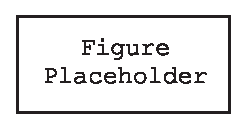
\includegraphics[width=4.6in]{c_cil0/ldmnblk.eps}
\caption{Long Dividend/Machine-Native Divisor Division In Functional Block Form}
\label{fig:ccil0:sidv0:sldm0:01}
\end{figure}

The following example illustrates how to apply the technique.

\begin{vworkexamplestatement}
\label{ex:ccil0:sidv0:sldm0:01}
Implement 32/8 unsigned division on the TMS370C8 processor, which is
characterized by a 16/8 division instruction.
\end{vworkexamplestatement}
\begin{vworkexampleparsection}{Solution}
It would be possible to prepare an implementation directly from
Figure \ref{fig:ccil0:sidv0:sldm0:01}:  however, it may be 
more instructive to work through a solution without the
aid of this figure.

In the case of the TMS370C8, the chunk size $Q$ is 8 bits; therefore
$Q=8$.  The problem statement indicates that we must accept 32-bit dividends;
therefore $P=32$.  Thus

\begin{equation}
\label{eq:ex:ccil0:sidv0:sldm0:01:001}
p = 2^{24} p_{[3]} + 2^{16} p_{[2]} + 2^{8} p_{[1]} + p_{[0]}
\end{equation}

\noindent{}and

\begin{equation}
\label{eq:ex:ccil0:sidv0:sldm0:01:002}
q = q_{[0]} .
\end{equation}

\noindent{}Thus the quotient and remainder we would like to determine,
$\lfloor p/q \rfloor$ and $p \bmod q$, can be obtained by repeated
application of (\ref{eq:ccil0:sidv0:sldm0:002}) as shown
in Equations (\ref{eq:ex:ccil0:sidv0:sldm0:01:003}) 
through (\ref{eq:ex:ccil0:sidv0:sldm0:01:011}).

\begin{equation}
\label{eq:ex:ccil0:sidv0:sldm0:01:003}
\frac{p}{q} 
=
\frac{2^{24} p_{[3]} + 2^{16} p_{[2]} + 2^{8} p_{[1]} + p_{[0]}}{q_{[0]}}
\end{equation}

\begin{equation}
\label{eq:ex:ccil0:sidv0:sldm0:01:004}
\frac{p}{q} 
=
2^{24} \frac{p_{[3]}}{q_{[0]}}
+
2^{16} \frac{p_{[2]}}{q_{[0]}}
+
2^{8} \frac{p_{[1]}}{q_{[0]}}
+
\frac{p_{[0]}}{q_{[0]}}
\end{equation}

\begin{equation}
\label{eq:ex:ccil0:sidv0:sldm0:01:005}
\frac{p}{q} 
=
2^{24} \left\lfloor{\frac{p_{[3]}}{q_{[0]}}}\right\rfloor
+
2^{24} \frac{(p_{[3]} \bmod q_{[0]})}{q_{[0]}}
+
2^{16} \frac{p_{[2]}}{q_{[0]}}
+
2^{8} \frac{p_{[1]}}{q_{[0]}}
+
\frac{p_{[0]}}{q_{[0]}}
\end{equation}

\begin{equation}
\label{eq:ex:ccil0:sidv0:sldm0:01:006}
\frac{p}{q} 
=
2^{24} \left\lfloor{\frac{p_{[3]}}{q_{[0]}}}\right\rfloor
+
2^{16} \frac{2^8 (p_{[3]} \bmod q_{[0]}) + p_{[2]}}{q_{[0]}}
+
2^{8} \frac{p_{[1]}}{q_{[0]}}
+
\frac{p_{[0]}}{q_{[0]}}
\end{equation}

\begin{eqnarray}
\label{eq:ex:ccil0:sidv0:sldm0:01:007}
\frac{p}{q} & = & 2^{24} \left\lfloor{\frac{p_{[3]}}{q_{[0]}}}\right\rfloor
+
2^{16} \left\lfloor{\frac{2^8 (p_{[3]} \bmod q_{[0]}) + p_{[2]}}{q_{[0]}}}\right\rfloor \\
\nonumber & + &
2^{16} \frac{(2^8 (p_{[3]} \bmod q_{[0]}) + p_{[2]}) \bmod q_{[0]}}{q_{[0]}}
+
2^{8} \frac{p_{[1]}}{q_{[0]}}
+
\frac{p_{[0]}}{q_{[0]}}
\end{eqnarray}

\begin{eqnarray}
\label{eq:ex:ccil0:sidv0:sldm0:01:008}
\frac{p}{q} & = & 2^{24} \left\lfloor{\frac{p_{[3]}}{q_{[0]}}}\right\rfloor
+
2^{16} \left\lfloor{\frac{2^8 (p_{[3]} \bmod q_{[0]}) + p_{[2]}}{q_{[0]}}}\right\rfloor \\
\nonumber & + &
2^{8} \frac{2^8((2^8 (p_{[3]} \bmod q_{[0]}) + p_{[2]}) \bmod q_{[0]}) + p_{[1]}}{q_{[0]}}
+
\frac{p_{[0]}}{q_{[0]}}
\end{eqnarray}

\begin{eqnarray}
\nonumber\frac{p}{q} & = & 2^{24} \left\lfloor{\frac{p_{[3]}}{q_{[0]}}}\right\rfloor
+
2^{16} \left\lfloor{\frac{2^8 (p_{[3]} \bmod q_{[0]}) + p_{[2]}}{q_{[0]}}}\right\rfloor \\
\label{eq:ex:ccil0:sidv0:sldm0:01:009}
 & + &
2^{8} \left\lfloor{\frac{2^8((2^8 (p_{[3]} \bmod q_{[0]}) + p_{[2]}) \bmod q_{[0]}) + p_{[1]}}{q_{[0]}}}\right\rfloor \\
\nonumber & + &
2^{8} \frac{(2^8((2^8 (p_{[3]} \bmod q_{[0]}) + p_{[2]}) \bmod q_{[0]}) + p_{[1]}) \bmod q_{[0]}}{q_{[0]}} \\
\nonumber & + &
\frac{p_{[0]}}{q_{[0]}}
\end{eqnarray}

\begin{eqnarray}
\nonumber\frac{p}{q} & = & 2^{24} \left\lfloor{\frac{p_{[3]}}{q_{[0]}}}\right\rfloor
+
2^{16} \left\lfloor{\frac{2^8 (p_{[3]} \bmod q_{[0]}) + p_{[2]}}{q_{[0]}}}\right\rfloor \\
\label{eq:ex:ccil0:sidv0:sldm0:01:010}
 & + &
2^{8} \left\lfloor{\frac{2^8((2^8 (p_{[3]} \bmod q_{[0]}) + p_{[2]}) \bmod q_{[0]}) + p_{[1]}}{q_{[0]}}}\right\rfloor \\
\nonumber & + &
\frac{2^8((2^8((2^8 (p_{[3]} \bmod q_{[0]}) + p_{[2]}) \bmod q_{[0]}) + p_{[1]}) \bmod q_{[0]}) + p_{[0]}}{q_{[0]}}
\end{eqnarray}

\begin{eqnarray}
\nonumber & \displaystyle \frac{p}{q} =  2^{24} \left\lfloor{\frac{p_{[3]}}{q_{[0]}}}\right\rfloor
+
2^{16} \left\lfloor{\frac{2^8 (p_{[3]} \bmod q_{[0]}) + p_{[2]}}{q_{[0]}}}\right\rfloor & \\
\label{eq:ex:ccil0:sidv0:sldm0:01:011}
 & \displaystyle + 
2^{8} \left\lfloor{\frac{2^8((2^8 (p_{[3]} \bmod q_{[0]}) + p_{[2]}) \bmod q_{[0]}) + p_{[1]}}{q_{[0]}}}\right\rfloor & \\
\nonumber & \displaystyle + 
\left\lfloor{\frac{2^8((2^8((2^8 (p_{[3]} \bmod q_{[0]}) + p_{[2]}) \bmod q_{[0]}) + p_{[1]}) \bmod q_{[0]}) + p_{[0]}}{q_{[0]}}}\right\rfloor + & \\
\nonumber 
& \displaystyle \frac{(2^8((2^8((2^8 (p_{[3]} \bmod q_{[0]}) + p_{[2]}) \bmod q_{[0]}) + p_{[1]}) \bmod q_{[0]}) + p_{[0]}) \bmod q_{[0]}}{q_{[0]}}
&
\end{eqnarray}

Note several things about the implementation suggested by 
(\ref{eq:ex:ccil0:sidv0:sldm0:01:011}):

\begin{itemize}
\item No addition or multiplication is required to calculate terms such as
      $2^8 (p_{[3]} \bmod q_{[0]}) + p_{[2]}$.  The high-order byte of the
      large dividend can be stuffed with $p_{[3]} \bmod q_{[0]}$ and
      the low-order byte with $p_{[2]}$.
\item No addition or multiplication is required to calculate the 
      result $\lfloor p/q \rfloor$.
      Note in (\ref{eq:ex:ccil0:sidv0:sldm0:01:011}) that the results are
      conveniently grouped as bytes with multipliers of $2^{24}$, 
      $2^{16}$, $2^8$, and $2^0=1$.  The terms can simply be placed into
      the appropriate byte, as a way of multplication by the appropriate
      power of 2.  Note also that each term is guaranteed to be
      $\in \{0, 1, 2, \ldots{} , 255\}$, by the argument presented
      earlier for (\ref{eq:ccil0:sidv0:sldm0:004}).  Thus, the
      addition will result in no carries, and each result byte can simply
      be placed directly in the correct memory location---addition is
      not necessary.
\item Four machine division instructions are required, and the remainder
      is produced automatically by the fourth instruction.
\end{itemize}

An implemenation for the TMS370C8 is supplied as Figure
\ref{fig:ex:ccil0:sidv0:sldm0:01:01}.  A block diagram of the data
flow for this implementation is supplied as 
Figure \ref{fig:ex:ccil0:sidv0:sldm0:01:02}.
\end{vworkexampleparsection}
\vworkexamplefooter{}

\begin{figure}
\begin{verbatim}
;Assume that byte memory locations p3, p2, p1, and p0 contain the
;32-bit unsigned dividend, and byte q0 contains the 8-bit unsigned
;divisor.  Assume also that the result quotient will be placed
;in byte memory locations d3, d2, d1, and d0; and that the
;remainder will be placed in the byte memory location r0.  Further
;assume that all memory locations are in the register file (near).
        CLR A        ;High-order chunk of large divisor
                     ;must be 0.
        MOV p3, B    ;Load the low-order chunk of divisor.
        DIV q0, A    ;Perform the first division.
        MOV A,  d3   ;Quotient becomes this part of the
                     ;result.
        MOV B,  A    ;Remainder becomes high-order chunk of
                     ;next division.
        MOV p2, B    ;Next byte becomes low-order chunk.
        DIV q0, A    ;Do the second division.
        MOV A,  d2   ;Quotient becomes this part of the
                     ;result.
        MOV B,  A    ;Remainder becomes high-order chunk of
                     ;next division.
        MOV p1, B    ;Next byte becomes low-order chunk.
        DIV q0, A    ;Do the third division.
        MOV A,  d1   ;Quotient becomes this part of the
                     ;result.
        MOV B,  A    ;Remainder becomes high-order chunk of
                     ;next division.
        MOV p0, B    ;Next byte becomes low-order chunk.
        DIV q0, A    ;Do the fourth division.
        MOV A,  d0   ;Quotient becomes this part of the
                     ;result.
        MOV B,  r0   ;This is the remainder, which could be used
                     ;for rounding.
\end{verbatim}
\caption{TMS370C8 Code Snippet Illustrating Unsigned 32/8 
         Division Using Unsigned 16/8
         Machine Instructions (Example \ref{ex:ccil0:sidv0:sldm0:01})}
\label{fig:ex:ccil0:sidv0:sldm0:01:01}
\end{figure}

\begin{figure}
\centering
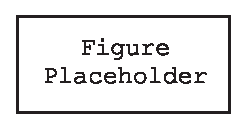
\includegraphics[width=4.6in]{c_cil0/t370dmp.eps}
\caption{Block Diagram Of Data Flow Of Figure \ref{fig:ex:ccil0:sidv0:sldm0:01:01}}
\label{fig:ex:ccil0:sidv0:sldm0:01:02}
\end{figure}


%%%%%%%%%%%%%%%%%%%%%%%%%%%%%%%%%%%%%%%%%%%%%%%%%%%%%%%%%%%%%%%%%%%%%%%%%%
%%%%%%%%%%%%%%%%%%%%%%%%%%%%%%%%%%%%%%%%%%%%%%%%%%%%%%%%%%%%%%%%%%%%%%%%%%
%%%%%%%%%%%%%%%%%%%%%%%%%%%%%%%%%%%%%%%%%%%%%%%%%%%%%%%%%%%%%%%%%%%%%%%%%%
\section{Miscellaneous Integer Mappings}
%Section tag: MIM0
\label{ccil0:smim0}

Embedded system work and ROM constraints often inspire a great deal
of cleverness in the selection of instructions to perform mappings or
tests.  In this section, we discuss integer mappings (i.e. functions)
for which economical implementations are known; and in the next section
(Section \ref{ccil0:smit0})
we discuss integer tests for which economical implementations are known.

To the best of our knowledge, there is no way to derive these mappings
and tests---they have been collected from many software developers and
come from human intuition and experience.


%%%%%%%%%%%%%%%%%%%%%%%%%%%%%%%%%%%%%%%%%%%%%%%%%%%%%%%%%%%%%%%%%%%%%%%%%%
%%%%%%%%%%%%%%%%%%%%%%%%%%%%%%%%%%%%%%%%%%%%%%%%%%%%%%%%%%%%%%%%%%%%%%%%%%
%%%%%%%%%%%%%%%%%%%%%%%%%%%%%%%%%%%%%%%%%%%%%%%%%%%%%%%%%%%%%%%%%%%%%%%%%%
\subsection{Lowest-Order Bit}
%Subsection tag: LIB0
\label{ccil0:smim0:slib0}

\index{lowest-order bit}
\index{least significant bit}

The mapping

\texttt{mask = x \& -x}

\noindent{}is the most economical way known to extract the 
lowest-order bit set in an integer \texttt{x}, or 
0 if no bits are set.\footnote{This mapping was contributed by 
David Baker (\texttt{bakerda@engin.umich.edu}) 
and Raul Selgado (\texttt{rselgado@visteon.com}).}  Since most processors have an instruction to form the
two's complement of an integer, this mapping usually requires only
two arithmetic instructions.

When implementing this mapping in assembly-language on processors without a
two's complement instruction, two other possible implementations are:

\begin{itemize}
\item \texttt{mask = x \& ($\sim$x + 1)}
\item \texttt{mask = x \& ((x \^{ } -1) + 1)}
\end{itemize}


%%%%%%%%%%%%%%%%%%%%%%%%%%%%%%%%%%%%%%%%%%%%%%%%%%%%%%%%%%%%%%%%%%%%%%%%%%
%%%%%%%%%%%%%%%%%%%%%%%%%%%%%%%%%%%%%%%%%%%%%%%%%%%%%%%%%%%%%%%%%%%%%%%%%%
%%%%%%%%%%%%%%%%%%%%%%%%%%%%%%%%%%%%%%%%%%%%%%%%%%%%%%%%%%%%%%%%%%%%%%%%%%
\section{Miscellaneous Integer Tests}
%Section tag: MIT0
\label{ccil0:smit0}

\subsection{Power Of 2}
%Subsection tag: PTW0
\label{ccil0:smit0:sptw0}

\index{power of two}
\index{2N@$2^N$}

The test

\texttt{(x \& (x-1) == 0) \&\& (x != 0)}

\noindent{}is the most economical way known to 
test whether an integer is a positive power of two 
(1, 2, 4, 8, 16, etc.).\footnote{The test appeared as part of
a discussion on 
the GMP mailing list in 2002.}


%%%%%%%%%%%%%%%%%%%%%%%%%%%%%%%%%%%%%%%%%%%%%%%%%%%%%%%%%%%%%%%%%%%%%%%%%%
%%%%%%%%%%%%%%%%%%%%%%%%%%%%%%%%%%%%%%%%%%%%%%%%%%%%%%%%%%%%%%%%%%%%%%%%%%
%%%%%%%%%%%%%%%%%%%%%%%%%%%%%%%%%%%%%%%%%%%%%%%%%%%%%%%%%%%%%%%%%%%%%%%%%%
\section{Exercises}

\begin{vworkexercisestatement}
\label{exe:ccil0:sexe0:01}
Show that any $m$-bit two's complement integer $u_{[m-1:0]}$ except
$-2^{m-1}$ can be negated by forming the one's complement, then adding one.
\end{vworkexercisestatement}



%%%%%%%%%%%%%%%%%%%%%%%%%%%%%%%%%%%%%%%%%%%%%%%%%%%%%%%%%%%%%%%%%%%%%%%%%%
%%%%%%%%%%%%%%%%%%%%%%%%%%%%%%%%%%%%%%%%%%%%%%%%%%%%%%%%%%%%%%%%%%%%%%%%%%
%%%%%%%%%%%%%%%%%%%%%%%%%%%%%%%%%%%%%%%%%%%%%%%%%%%%%%%%%%%%%%%%%%%%%%%%%%
\vfill
\noindent\begin{figure}[!b]
\noindent\rule[-0.25in]{\textwidth}{1pt}
\begin{tiny}
\begin{verbatim}
$HeadURL: svn://localhost/dtapublic/pubs/books/ucbka/trunk/c_cil0/c_cil0.tex $
$Revision: 277 $
$Date: 2019-08-12 22:35:39 -0400 (Mon, 12 Aug 2019) $
$Author: dashley $
\end{verbatim}
\end{tiny}
\noindent\rule[0.25in]{\textwidth}{1pt}
\end{figure}

%%%%%%%%%%%%%%%%%%%%%%%%%%%%%%%%%%%%%%%%%%%%%%%%%%%%%%%%%%%%%%%%%%%%%%%%%%
%
%End of file C_CIL0.TEX


%Chapter:  Rational Approximation
%$Header: svn://localhost/dtapublic/pubs/books/ucbka/trunk/c_rat0/c_rat0.tex 278 2019-08-14 23:10:36Z dashley $

\chapter{Rational Linear Approximation}

\label{crat0}

\beginchapterquote{``Die ganzen Zahlen hat der liebe Gott gemacht,
                   alles andere ist Menschenwerk.''\footnote{German
                   language: God made the integers; everything
                   else was made by man.}}
                   {Leopold Kronecker}

%%%%%%%%%%%%%%%%%%%%%%%%%%%%%%%%%%%%%%%%%%%%%%%%%%%%%%%%%%%%%%%%%%%%%%%%%%
%%%%%%%%%%%%%%%%%%%%%%%%%%%%%%%%%%%%%%%%%%%%%%%%%%%%%%%%%%%%%%%%%%%%%%%%%%
%%%%%%%%%%%%%%%%%%%%%%%%%%%%%%%%%%%%%%%%%%%%%%%%%%%%%%%%%%%%%%%%%%%%%%%%%%
\section{Introduction}
%Section tag: INT0
\label{crat0:sint0}

In this chapter, we consider practical applications of
rational approximation.
Chapters \cfryzeroxrefhyphen\ref{cfry0} and \ccfrzeroxrefhyphen\ref{ccfr0}
have presented algorithms for finding 
the closest rational numbers to an arbitrary real number,
subject to constraints on the numerator and denominator.
The basis of these algorithms is complex and comes from number theory, and so
these algorithms and their basis have been presented in separate chapters.

In Section \ref{crat0:srla0}, rational linear approximation itself
and associated error bounds are presented.  By \emph{rational linear
approximation} we mean simply the approximation of a line
$y = r_I x$ ($y, r_I, x \in \vworkrealset$) by a line

\begin{equation}
\label{eq:crat0:sint0:01}
y = \left\lfloor
    \frac{h \lfloor x \rfloor + z}{k}
    \right\rfloor ,
\end{equation}

\noindent{}where we choose $h/k \approx r_I$ and optionally choose $z$ to 
shift the error introduced.  Note that (\ref{eq:crat0:sint0:01}) is
very economical for microcontroller instruction sets, since only integer
arithmetic is required.  We may choose $h/k$ from a Farey series (see
Chapters \cfryzeroxrefhyphen\ref{cfry0} and \ccfrzeroxrefhyphen\ref{ccfr0}), or 
we may choose a ratio $h/2^q$ so that the division in (\ref{eq:crat0:sint0:01})
can be implemented
by a bitwise right shift.

Section \ref{crat0:srla0} discusses linear rational approximation
in general, with a special eye on error analysis.

Section \ref{crat0:spwi0} discusses piecewise linear rational approximation,
which is the approximation of a curve or complex mapping by a 
number of joined line segments.

Section \ref{crat0:sfdv0} discusses frequency division and rational counting.
Such techniques share the same mathematical framework as rational linear
approximation, and as with rational linear approximation the ratio
involved may be chosen from a Farey series or with a denominator of $2^q$, depending
on the algorithm employed.

Section \ref{crat0:sbla0} discusses Bresenham's classic line algorithm,
which is a practical application of rational linear approximation.

%%%%%%%%%%%%%%%%%%%%%%%%%%%%%%%%%%%%%%%%%%%%%%%%%%%%%%%%%%%%%%%%%%%%%%%%%%
%%%%%%%%%%%%%%%%%%%%%%%%%%%%%%%%%%%%%%%%%%%%%%%%%%%%%%%%%%%%%%%%%%%%%%%%%%
%%%%%%%%%%%%%%%%%%%%%%%%%%%%%%%%%%%%%%%%%%%%%%%%%%%%%%%%%%%%%%%%%%%%%%%%%%
\section{Rational Linear Approximation}
%Section tag: RLA0
\label{crat0:srla0}

It occurs frequently in embedded software design that one wishes to
implement a linear scaling from a domain to a range of the form

\begin{equation}
\label{eq:crat0:srla0:01}
f(x) = r_I x ,
\end{equation}

\noindent{}where $r_I$ is the \emph{ideal}


%%%%%%%%%%%%%%%%%%%%%%%%%%%%%%%%%%%%%%%%%%%%%%%%%%%%%%%%%%%%%%%%%%%%%%%%%%
%%%%%%%%%%%%%%%%%%%%%%%%%%%%%%%%%%%%%%%%%%%%%%%%%%%%%%%%%%%%%%%%%%%%%%%%%%
%%%%%%%%%%%%%%%%%%%%%%%%%%%%%%%%%%%%%%%%%%%%%%%%%%%%%%%%%%%%%%%%%%%%%%%%%%
\subsection{Model Functions}
%Section tag: mfu0
\label{crat0:srla0:smfu0}

In general, we seek to approximate the ideal function


\noindent{}by some less ideal function where

\begin{itemize}
\item $r_A \neq r_I$, although we seek to choose $r_A \approx r_I$.
\item The input to the function, $x$, may already contain
      quantization error.
\item Although $r_I x \in \vworkrealsetnonneg$, we must choose
      an integer as the function output. 
\end{itemize}

In modeling quantization error, we use the floor function\index{floor function}
($\lfloor\cdot\rfloor$)
for algebraic simplicity.  The floor function precisely 
describes the behavior of integer division instructions (where 
remainders are discarded), but may not describe other sources of 
quantization, such as quantization that occurs in A/D conversion.
However, techniques identical to those presented in this
section may be used when quantization is not best described 
by the floor function, and these results are left to the reader.

Traditionally, because addition of integers is an inexpensive
machine operation, a parameter $z \in \vworkintset$ may optionally 
be added to the product $hx$ in order to round or otherwise
shift the result.

If $x$ is assumed to be without error, the ideal function is
given by (\ref{eq:crat0:srla0:smfu0:01}), whereas the function
that can be economically implemented is

\begin{equation}
\label{eq:crat0:srla0:smfu0:02}
g(x) = \left\lfloor \frac{hx + z}{k} \right\rfloor
=
\left\lfloor r_A x + \frac{z}{k} \right\rfloor .
\end{equation}

If, on the other hand, $x$ may be already quantized,
the function that can actually be implemented is

\begin{equation}
\label{eq:crat0:srla0:smfu0:03}
h(x) = \left\lfloor \frac{h \lfloor x \rfloor + z}{k} \right\rfloor
=
\left\lfloor r_A \lfloor x \rfloor + \frac{z}{k} \right\rfloor .
\end{equation}



%%%%%%%%%%%%%%%%%%%%%%%%%%%%%%%%%%%%%%%%%%%%%%%%%%%%%%%%%%%%%%%%%%%%%%%%%%
%%%%%%%%%%%%%%%%%%%%%%%%%%%%%%%%%%%%%%%%%%%%%%%%%%%%%%%%%%%%%%%%%%%%%%%%%%
%%%%%%%%%%%%%%%%%%%%%%%%%%%%%%%%%%%%%%%%%%%%%%%%%%%%%%%%%%%%%%%%%%%%%%%%%%
\section[\protect\mbox{\protect$h/2^q$} and  \protect\mbox{\protect$2^q/k$} Rational Linear Approximation]
        {\protect\mbox{\protect\boldmath$h/2^q$} and \protect\mbox{\protect\boldmath$2^q/k$} Rational Linear Approximation}
%Section tag: HQQ0
\label{crat0:shqq0}

\index{h/2q@$h/2^q$ rational linear approximation}
\index{rational linear approximation!h/2q@$h/2^q$}
The algorithms presented in
Chapters \cfryzeroxrefhyphen\ref{cfry0} and \ccfrzeroxrefhyphen\ref{ccfr0}
will always provide the rational number $h/k$ closest to
an arbitrary real number $r_I$ subject to the constraints
$h \leq h_{MAX}$ and $k \leq k_{MAX}$.

However, because shifting in order
to implement multiplication or division by a power of 2 
is at least as fast (and often \emph{much} faster)
on all processors as arbitrary multiplication or division, 
and because not all processors have multiplication and division instructions,
it is worthwhile to examine choosing $h/k$ so that either $h$ or $k$ are 
powers of 2.

There are thus three rational linear approximation techniques to be
examined:

\begin{enumerate}
\item \emph{$h/k$ rational linear approximation}, in which an arbitrary
      $h \leq h_{MAX}$ and an arbitrary $k \leq k_{MAX}$ are used,
	  with $r_A = h/k$.  $h$ and $k$ can be chosen using the algorithms
	  presented in Chapters \cfryzeroxrefhyphen\ref{cfry0} and \ccfrzeroxrefhyphen\ref{ccfr0}.
	  Implementation of this technique would most often involve a single integer
	  multiplication instruction to form the product $hx$, followed by an optional single
	  addition instruction to form the sum $hx+z$, and then 
	  followed by by a single division instruction
	  to form the quotient $\lfloor (hx+z)/k \rfloor$.  Implementation may also less commonly involve
	  multiplication, addition, and division of operands too large to be processed
	  with single machine instructions.
\item \emph{$h/2^q$ rational linear approximation}, in which an arbitrary 
      $h \leq h_{MAX}$ and an integral power of two $k=2^q$ are used, with
	  $r_A = h/2^q$.
	  Implementation of this technique would most often involve a single integer
	  multiplication instruction to form the product $hx$, followed by an optional single
	  addition instruction to form the sum $hx+z$, and then 
	  followed by right shift instruction(s)
	  to form the quotient $\lfloor (hx+z)/2^q \rfloor$.  Implementation may also less commonly involve
	  multiplication, addition, and right shift of operands too large to be processed
	  with single machine instructions.
\item \emph{$2^q/k$ rational linear approximation}, in which an integral
      power of two $h=2^q$ and an arbitrary $k \leq k_{MAX}$ are used, with
	  $r_A = 2^q/k$.
	  Implementation of this technique would most often involve left shift
	  instruction(s) to form the product $2^qx$, followed by an optional single
	  addition instruction to form the sum $2^qx+z$, and then 
	  followed by a single division instruction to form 
	  the quotient $\lfloor (2^qx+z)/k \rfloor$.  Implementation may also less 
	  commonly involve
	  left shift, addition, and division of operands too large to be processed
	  with single machine instructions.
\end{enumerate}

We use the nomenclature ``\emph{$h/k$ rational linear approximation}'',
``\emph{$h/2^q$ rational linear approximation}'', and 
``\emph{$2^q/k$ rational linear approximation}'' to identify the three
techniques enumerated above.


%%%%%%%%%%%%%%%%%%%%%%%%%%%%%%%%%%%%%%%%%%%%%%%%%%%%%%%%%%%%%%%%%%%%%%%%%%
%%%%%%%%%%%%%%%%%%%%%%%%%%%%%%%%%%%%%%%%%%%%%%%%%%%%%%%%%%%%%%%%%%%%%%%%%%
%%%%%%%%%%%%%%%%%%%%%%%%%%%%%%%%%%%%%%%%%%%%%%%%%%%%%%%%%%%%%%%%%%%%%%%%%%
\subsection{Integer Arithmetic and Processor Instruction Set Characteristics}
%Subsection tag: pis0
\label{crat0:shqq0:pis0}

The following observations about integer arithmetic and about processors 
used in embedded control can be made:

\begin{enumerate}
\item \label{enum:crat0:shqq0:pis0:01:01a}
      \emph{Shifting is the fastest method of integer multiplication or division
	  (by $2^q$ only),
      followed by utilization of the processor multiplication or division instructions (for arbitrary
	  operands), 
	  followed by software implementation of multiplication or division (for arbitrary operands).}
	  Relative costs vary depending on the processor, but the monotonic
	  ordering always holds.
	  $h/2^q$ and $2^q/k$ rational linear 
	  approximation are thus worthy of investigation.  (Note also that in many practical 
	  applications of $h/2^q$ and $2^q/k$ rational linear approximation, 
	  the required shift is performed by
      addressing the operand with an offset,
	  and so has no cost.)
\item \label{enum:crat0:shqq0:pis0:01:01b}
      \emph{Shifting is $O(N)$ (where $N$ is the number of bits in the argument), 
	  but both
	  multiplication and division are $O(N^2)$ for 
	  practical\footnote{\index{Karatsuba multiplication}Karatsuba 
	  multiplication, for example, is
	  $O(N^{\log_2 3}) \approx O(N^{1.58}) \ll O(N^2)$.  However, Karatsuba
	  multiplication cannot be applied economically to the small
	  operands that typically occur in embedded control work.  It would
	  be rare in embedded control applications
	  for the length of a multiplication operand to exceed four 
	  times the length that is accommodated by a machine instruction; and this
	  is far below the threshold at which Karatsuba multiplication is
	  economical.  Thus, for all intents and purposes in embedded control work,
	  multiplication is $O(N^2)$.} operands (where 
	  $N$ is the number of bits in each 
	  operand).}  It follows that $2^q/k$ and $h/2^q$ rational 
	  linear approximation
	  will scale to large operands better than $h/k$ rational linear approximation.
\item \label{enum:crat0:shqq0:pis0:01:02a}
      \emph{Integer division instructions take as long or longer than
      integer multiplication instructions.}  In designing digital logic
	  to implement basic integer arithmetic, division is the operation most difficult
      to perform economically.\footnote{For some processors, the penalty is extreme.
	  For example, on the NEC V850 (a RISC processor), 
	  a division requires 36 clock cycles,
	  whereas multiplication, addition, and subtraction each effectively 
	  require 1 clock cycle.}
	  It follows that multiplication using operands that exceed the machine's word size
	  is often far less expensive than division using operands that exceed the 
	  machine's word size. 
\item \label{enum:crat0:shqq0:pis0:01:03a}
      \emph{All processors that have an integer division instruction also
      have an integer multiplication instruction.}  
	  Phrased
	  differently, no processor has an integer division instruction but no
	  integer multiplication instruction.
\end{enumerate}

Enumerated items
(\ref{enum:crat0:shqq0:pis0:01:01a}) through
(\ref{enum:crat0:shqq0:pis0:01:03a}) above lead to the following conclusions.

\begin{enumerate}
\item $h/2^q$ rational linear approximation is likely to be implementable 
      more efficiently on most processors than $h/k$ rational linear approximation.
	  (\emph{Rationale:}  shift instruction(s) or accessing a 
	  memory address with an offset
	  is
	  likely to be more economical than division, particularly if $k$ would exceed 
	  the native
	  operand size of the processor.)
\item $h/2^q$ rational linear approximation is likely to be a more useful
      technique than $2^q/k$ rational linear approximation.
	  (\emph{Rationale:}  the generally high cost of division compared to 
	  multiplication, and the existence of processors that possess a multiplication 
	  instruction but no division instruction.)
\end{enumerate}


%%%%%%%%%%%%%%%%%%%%%%%%%%%%%%%%%%%%%%%%%%%%%%%%%%%%%%%%%%%%%%%%%%%%%%%%%%
%%%%%%%%%%%%%%%%%%%%%%%%%%%%%%%%%%%%%%%%%%%%%%%%%%%%%%%%%%%%%%%%%%%%%%%%%%
%%%%%%%%%%%%%%%%%%%%%%%%%%%%%%%%%%%%%%%%%%%%%%%%%%%%%%%%%%%%%%%%%%%%%%%%%%
\subsection[Design Procedure For \protect\mbox{\protect$h/2^q$} Rational Linear Approximations]
           {Design Procedure For \protect\mbox{\protect\boldmath$h/2^q$} Rational Linear Approximation}
%Subsection tag: dph0
\label{crat0:shqq0:dph0}

An $h/2^q$ rational linear approximation is parameterized by:

\begin{itemize}
\item The unsigned or signed nature of $h$ and $x$. (Rational linear approximations
      may involve either signed or unsigned domains and ranges.  Furthermore,
	  signed integers may be maintained using either 2's-complement
	  or sign-magnitude representation, and the processor instruction set
	  may or may not directly support signed multiplication.)
\item $r_I$, the real number we wish to approximate by $r_A = h/2^q$.
\item $x_{MAX}$, the maximum possible value of the input argument $x$.  (Typically,
      software contains a test to clip the output if $x > x_{MAX}$.)
\item $w_h$, the width in bits allowed for $h$.  (Typically, $w_h$ is 
      the maximum operand size of a machine multiplication instruction.)
\item $w_r$, the width in bits allowed for the result $hx$.  (Typically,
      $w_r$ is the maximum result size of a machine multiplication instruction.)
\item The rounding mode when choosing $h$ (and thus effectively $r_A$) 
      based on $r_I$.  It is common to choose the
      closest value, 
	  $r_A=\lfloor r_I 2^q + 1/2 \rfloor/2^q$
	  or
	  $r_A=\lceil r_I 2^q - 1/2 \rceil/2^q$,
	  but other choices are possible.
\item The rounding mode for the result (i.e. the choice of $z$ in
      Eq. \ref{eq:crat0:sint0:01}).
\end{itemize}

This section develops a design procedure for $h/2^q$ rational linear
approximations with the most typical set of assumptions:  unsigned arithmetic,
$r_A=\lfloor r_I 2^q + 1/2 \rfloor/2^q$,
and $z=0$.  Design procedures for other scenarios are presented as exercises.

By definition, $h$ is constrained in two ways:

\begin{equation}
\label{eq:crat0:shqq0:dph0:00}
h \leq 2^{w_h} - 1
\end{equation}

\noindent{}and

\begin{equation}
\label{eq:crat0:shqq0:dph0:01}
h \leq \frac{2^{w_r} - 1}{x_{MAX}} .
\end{equation}

\noindent{}(\ref{eq:crat0:shqq0:dph0:00}) comes directly from the
requirement that $h$ fit in $w_h$ bits.
(\ref{eq:crat0:shqq0:dph0:01}) comes directly from the requirement
that $hx$ fit in $w_r$ bits.
(\ref{eq:crat0:shqq0:dph0:00}) and (\ref{eq:crat0:shqq0:dph0:01})
may be combined to form one inequality:

\begin{equation}
\label{eq:crat0:shqq0:dph0:02}
h \leq \min \left( { 2^{w_h} - 1, \frac{2^{w_r} - 1}{x_{MAX}} } \right ) .
\end{equation}

If $q$ is known, the choice of $h$ that will be made so as to minimize
$|r_A-r_I| = |h/2^q - r_I|$ is

\begin{equation}
\label{eq:crat0:shqq0:dph0:03}
h=\left\lfloor r_I 2^q + \frac{1}{2} \right\rfloor .
\end{equation}

\noindent{}It is required that the choice of $h$ specified by
(\ref{eq:crat0:shqq0:dph0:03}) meet 
(\ref{eq:crat0:shqq0:dph0:02}).  Making the most pessimistic 
assumption about the rounding of $h$ and substituting into
(\ref{eq:crat0:shqq0:dph0:02}) leads to

\begin{equation}
\label{eq:crat0:shqq0:dph0:04}
r_I 2^q + \frac{1}{2}
\leq
\min \left( { 2^{w_h} - 1, \frac{2^{w_r} - 1}{x_{MAX}} } \right ) .
\end{equation}

\noindent{}Isolating $q$ in (\ref{eq:crat0:shqq0:dph0:04})
yields

\begin{equation}
\label{eq:crat0:shqq0:dph0:05}
2^q 
\leq
\frac{\min \left( { 2^{w_h} - 1, \frac{2^{w_r} - 1}{x_{MAX}} } \right ) - \frac{1}{2}}
{r_I}.
\end{equation}

\noindent{}Solving 
(\ref{eq:crat0:shqq0:dph0:05})
for maximum value of $q$ that meets the constraint yields

\begin{equation}
\label{eq:crat0:shqq0:dph0:06}
q=
\left\lfloor
{
\log_2
\left(
{
\frac{\min \left( { 2^{w_h} - 1, \frac{2^{w_r} - 1}{x_{MAX}} } \right ) - \frac{1}{2}}{r_I}
}
\right)
}
\right\rfloor .
\end{equation}

\noindent{}(\ref{eq:crat0:shqq0:dph0:06})
can be rewritten for easier calculation using most calculators (which do
not allow the direct evaluation of base-2 logarithms):

\begin{equation}
\label{eq:crat0:shqq0:dph0:07}
q=
\left\lfloor
\frac
{
{
\ln
\left(
{
\frac{\min \left( { 2^{w_h} - 1, \frac{2^{w_r} - 1}{x_{MAX}} } \right ) - \frac{1}{2}}{r_I}
}
\right)
}
}
{\ln 2}
\right\rfloor .
\end{equation}

\noindent{}Once $q$ is established using (\ref{eq:crat0:shqq0:dph0:07}),
$h$ can be calculated using (\ref{eq:crat0:shqq0:dph0:03}).

In embedded control work (as well as in operating system internals),
$h/2^q$ rational linear approximations are often used in conjunction with
tabulated constants or calibratable parameters
where each constant or calibratable parameter may vary over a range of
$[0, r_I]$, and where $r_I$ is the value used in the design procedure
presented above.  In these applications, the values of $h$ are
tabulated, but $q$ is invariant (usually hard-coded)
and is chosen at design time based on the upper bound $r_I$ 
of the interval $[0, r_I]$ in which each tabulated constant or calibratable
parameter will fall.  With $q$ fixed,
$r_A$ can be adjusted in steps of $1/2^q$.

If $r_I$ is invariant, a final design step may be to reduce the rational
number $h/2^q$ by dividing some or all occurrences of 2 as a factor from both the
numerator and denominator.  With some processors and in some applications, this
may save execution time by reducing the number of shift instructions that 
must be executed, reducing the execution time of the shift instructions
that are executed, or allowing shifting via offset addressing.
For example, on a byte-addressible machine, if the design procedure 
yields $h=608$ and $q=10$, it may be desirable to divide both $h$ and $2^q$ by 4 to
yield $h=152$ and $q=8$, as this allows the shift by 8 to be done by fetching 
alternate bytes (rather than by actual shifting).  In other applications, it may
be desirable to remove \emph{all} occurrences of 2 as a prime factor
from $h$.

For an invariant $r_I$, a suitable design procedure is:

\begin{enumerate}
\item Choose $q$ using (\ref{eq:crat0:shqq0:dph0:07}).
\item With $q$ fixed, choose $h$ using (\ref{eq:crat0:shqq0:dph0:03}).
\item If economies can be achieved on the target processor, 
      examine the possibility of removing some or all occurrences
	  of 2 as a prime factor from $h$ and decreasing $q$.
\end{enumerate}

For tabulated or calibratable constants in the
interval $[0,r_I]$, a suitable design procedure is to use the 
procedure presented immediately above but without the third step.
Each tabulated value of $h$ is chosen using (\ref{eq:crat0:shqq0:dph0:03}).

%%%%%%%%%%%%%%%%%%%%%%%%%%%%%%%%%%%%%%%%%%%%%%%%%%%%%%%%%%%%%%%%%%%%%%%%%%
%%%%%%%%%%%%%%%%%%%%%%%%%%%%%%%%%%%%%%%%%%%%%%%%%%%%%%%%%%%%%%%%%%%%%%%%%%
%%%%%%%%%%%%%%%%%%%%%%%%%%%%%%%%%%%%%%%%%%%%%%%%%%%%%%%%%%%%%%%%%%%%%%%%%%
\subsection[Design Procedure For \protect\mbox{\protect$2^q/k$} Rational Linear Approximations]
           {Design Procedure For \protect\mbox{\protect\boldmath$2^q/k$} Rational Linear Approximation}
%Subsection tag: dpk0
\label{crat0:shqq0:dpk0}

TBD.

%%%%%%%%%%%%%%%%%%%%%%%%%%%%%%%%%%%%%%%%%%%%%%%%%%%%%%%%%%%%%%%%%%%%%%%%%%
%%%%%%%%%%%%%%%%%%%%%%%%%%%%%%%%%%%%%%%%%%%%%%%%%%%%%%%%%%%%%%%%%%%%%%%%%%
%%%%%%%%%%%%%%%%%%%%%%%%%%%%%%%%%%%%%%%%%%%%%%%%%%%%%%%%%%%%%%%%%%%%%%%%%%
\section{Piecewise Rational Linear Approximation}
%Section tag: PWI0
\label{crat0:spwi0}

TBD.

%%%%%%%%%%%%%%%%%%%%%%%%%%%%%%%%%%%%%%%%%%%%%%%%%%%%%%%%%%%%%%%%%%%%%%%%%%
%%%%%%%%%%%%%%%%%%%%%%%%%%%%%%%%%%%%%%%%%%%%%%%%%%%%%%%%%%%%%%%%%%%%%%%%%%
%%%%%%%%%%%%%%%%%%%%%%%%%%%%%%%%%%%%%%%%%%%%%%%%%%%%%%%%%%%%%%%%%%%%%%%%%%
\section[Frequency Division And Rational Counting]
        {Frequency Division And Rational Counting Techniques}
%Section tag: FDV0
\label{crat0:sfdv0}

\index{frequency division}\index{rational counting}\index{counting}%
Often, software must ``divide down'' an execution rate.  For example,
an interrupt service routine may be scheduled by hardware every
10ms, but may perform useful processing only every 50ms.  This requires
that the ISR maintain a counter and only perform useful processing
every fifth invocation.  This section deals with counting strategies
used to achieve invocation frequency division and other similar results.

Frequency division and
rational counting techniques presented in this section find application
primarily in the following scenarios:

\begin{itemize}
\item ISRs and other software components which must divide down
      their invocation rate.
\item Pulse counting and scaling from encoders and other
      similar systems.
\item The correction of inaccuracies in timebases (such as crystals
      which oscillate at a frequency different than the
      nominal rate).
\end{itemize}

Because the techniques presented must be usable with inexpensive 
microcontrollers, such techniques must meet these constraints:

\begin{enumerate}
\item \label{enum:01:crat0:sfdv0:econex}
      The counting techniques must be economical to execute on
      an inexpensive microcontroller.
\item \label{enum:01:crat0:sfdv0:econcccalc}
      An inexpensive microcontroller must be capable of calculating any
      constants used as limits in counting (i.e. it cannot necessarily
      be assumed that a more powerful computer calculates these constants,
      and it cannot be assumed that these limits do not change on the fly).
\end{enumerate}

In this section, we analyze the behavior of several types of
rational counting algorithms, supplied as Algorithms
\ref{alg:crat0:sfdv0:01a}
through
\ref{alg:crat0:sfdv0:02a}.

\begin{algorithm}
\begin{verbatim}
/* The constants K1 through K4, which parameterize  the   */
/* counting behavior, are assumed assigned elsewhere in   */
/* the code.  The solution is analyzed in terms of the    */
/* parameters K1 through K4.                              */
/*                                                        */
/* We also place the following restrictions on K1 through */
/* K4:                                                    */
/*    K1  :  K1 <= K3 - K2.                               */
/*    K2  :  K4 >  K2 > 0.                                */
/*    K3  :  No restrictions.                             */
/*    K4  :  K4 >  K2 > 0.                                */

void base_rate_sub(void)
   {
   static int state = K1;

   state += K2;

   if (state >= K3)
      {
      state -= K4;
      A();
      }
   }
\end{verbatim}
\caption{Rational Counting Algorithm For $K_2/K_4 < 1$}
\label{alg:crat0:sfdv0:01a}
\end{algorithm}

\begin{algorithm}
\begin{verbatim}
/* The constants K1 through K4, which parameterize  the   */
/* counting behavior, are assumed assigned elsewhere in   */
/* the code.  The solution is analyzed in terms of the    */
/* parameters K1 through K4.                              */
/*                                                        */
/* We also place the following restrictions on K1 through */
/* K4:                                                    */
/*    K1  :  K1 <= K3 - K2.                               */
/*    K2  :  K2 >  0.                                     */
/*    K3  :  No restrictions.                             */
/*    K4  :  K4 >  0.                                     */

void base_rate_sub(void)
   {
   static int state = K1;

   state += K2;                          

   while (state >= K3)  
      {
      state -= K4;
      A();
      }
   }
\end{verbatim}
\caption{Rational Counting Algorithm For $K_2/K_4 \geq 1$}
\label{alg:crat0:sfdv0:01b}
\end{algorithm}

\begin{algorithm}
\begin{verbatim}
/* The constants K1, K2, and K4, which parameterize the   */
/* counting behavior, are assumed assigned elsewhere in   */
/* the code.  The solution is analyzed in terms of the    */
/* parameters K1 through K4.                              */
/*                                                        */
/* We also place the following restrictions on K1, K2,    */
/* and K4:                                                */
/*    K1  :  K1 >= 0.                                     */
/*    K2  :  K4 >  K2 > 0.                                */
/*    K4  :  K4 >  K2 > 0.                                */
/*                                                        */
/* Special thanks to Chuck B. Falconer (of the            */
/* comp.arch.embedded newsgroup) for this rational        */
/* counting algorithm.                                    */
/*                                                        */
/* Note below that the test against K3 does not exist,    */
/* instead a test against zero is used, which many        */
/* machine instruction sets will do as part of the        */
/* subtraction (but perhaps this needs to be coded in     */
/* A/L).  This saves machine code and also eliminates     */
/* one unnecessary degree of freedom (K3).                */

void base_rate_sub(void)
   {
   static int state = K1;

   if ((state -= K2) < 0)
      {
      state += K4;
      A();
      }
   }
\end{verbatim}
\caption{Zero-Test Rational Counting Algorithm For $K_2/K_4 < 1$}
\label{alg:crat0:sfdv0:01c}
\end{algorithm}

\begin{algorithm}
\begin{verbatim}
;Special thanks to John Larkin (of the comp.arch.embedded
;newsgroup) for this rational counting algorithm.
;
;This is the TMS-370C8 assembly-language version of the 
;algorithm.  The algorithm is parameterized solely by
;K1 and K2, with no restrictions on their values, because
;the values are naturally constrained by the data types.  
;K1, which is the initial value of "state", is assumed
;assigned elsewhere.  The snippet shown here uses only
;K2.
          MOV  state, A     ;Get "state".
          ADD  #K2,   A     ;Increase by K2.  Carry flag
                            ;will be set if rollover to or
                            ;past zero.
          PUSH ST           ;Save carry flag.
          MOV  A,     state ;Move new value back.
          POP  ST           ;Restore carry flag.
          JNC  done         ;If didn't roll, don't run sub.
          CALL A_SUBROUTINE ;Run sub.
done:

/* This is the 'C' version of the algorithm.  It is not   */
/* as easy or efficient in 'C' to detect rollover.        */

void base_rate_sub(void)
   {
   static unsigned int state = K1;
   unsigned int old_state;

   old_state  = state;
   state     += K2;
   if (state < old_state)
      {
      A();
      }
   }
\end{verbatim}
\caption{$2^q$ Rollover Rational Counting Algorithm}
\label{alg:crat0:sfdv0:01d}
\end{algorithm}

\begin{algorithm}
\begin{verbatim}
/* The constants K1 through K4, which parameterize  the   */
/* counting behavior, are assumed assigned elsewhere in   */
/* the code.  The solution is analyzed in terms of the    */
/* parameters K1 through K4.                              */
/*                                                        */
/* We also place the following restrictions on K1 through */
/* K4:                                                    */
/*    K1  :  K1 <= K3.                                    */
/*    K2  :  K2 >  0.                                     */
/*    K3  :  No restrictions.                             */
/*    K4  :  K4 >  0.                                     */

void base_rate_sub(void)
   {
   static unsigned int state = K1;

   if (state >= K3)
      {
      state -= K4;
      A();
      }
   else
      {
      state += K2;
      B();
      }
   }
\end{verbatim}
\caption{Rational Counting Algorithm With \texttt{else} Clause}
\label{alg:crat0:sfdv0:02a}
\end{algorithm}


%%%%%%%%%%%%%%%%%%%%%%%%%%%%%%%%%%%%%%%%%%%%%%%%%%%%%%%%%%%%%%%%%%%%%%%%%%
%%%%%%%%%%%%%%%%%%%%%%%%%%%%%%%%%%%%%%%%%%%%%%%%%%%%%%%%%%%%%%%%%%%%%%%%%%
%%%%%%%%%%%%%%%%%%%%%%%%%%%%%%%%%%%%%%%%%%%%%%%%%%%%%%%%%%%%%%%%%%%%%%%%%%
\subsection[Properties Of Algorithm \ref{alg:crat0:sfdv0:01a}]
           {Properties Of Rational Counting Algorithm \ref{alg:crat0:sfdv0:01a}}
%Section tag: PRC0
\label{crat0:sfdv0:sprc0}

Algorithm \ref{alg:crat0:sfdv0:01a} 
is used frequently in microcontroller
software.  A base rate subroutine\footnote{For brevity, we usually
call this just the \emph{base subroutine}.} (named ``\texttt{base\_rate\_sub()}''
in the algorithm) is called at a periodic rate, and subroutine
``\texttt{A()}'' is called at a lesser rate.
We are interested in determining the relationships between the rates
as a function of $K_1$, $K_2$, $K_3$, and $K_4$; and we are interested
in developing other properties.

Notationally when analyzing rational counting algorithms, we agree
that $state_n$ denotes the value of the \texttt{state} variable 
after the $n$th invocation and before the $n+1$'th invocation
of the base rate subroutine.
Using this convention with Algorithm \ref{alg:crat0:sfdv0:01a}, 
$state_0 = K_1$.\footnote{Algorithm \ref{alg:crat0:sfdv0:01a} 
requires a knowledge of
`C' to fully understand.  The \texttt{static} keyword ensures that the
variable \texttt{state} is initialized only once, at the time the program
is loaded.  \texttt{state} is \emph{not} initialized each time the 
base subroutine runs.}

We can first easily derive the number of initial invocations of
the base subroutine before ``\texttt{A()}'' is called for the first 
time.

\begin{vworklemmastatement}
\label{lem:crat0:sfdv0:sprc0:01}
$N_{STARTUP}$, the number of invocations of the base subroutine
in Algorithm \ref{alg:crat0:sfdv0:01a} before ``\texttt{A()}'' is called
for the first time, is given by

\begin{equation}
\label{eq:lem:crat0:sfdv0:sprc0:01:01}
N_{STARTUP} = 
\left\lceil
{
\frac{-K_1 - K_2 + K_3}{K_2}
}
\right\rceil .
\end{equation} 
\end{vworklemmastatement}
\begin{vworklemmaproof}
The value of \texttt{state} after the $n$th invocation
is $state_n = K_1 + n K_2$.  In order for the test in the 
\texttt{if()} statement not to be met, we require that

\begin{equation}
\label{eq:lem:crat0:sfdv0:sprc0:01:02}
K_1 + n K_2 < K_3
\end{equation} 

\noindent{}or equivalently that

\begin{equation}
\label{eq:lem:crat0:sfdv0:sprc0:01:03}
n < \frac{K_3 - K_1}{K_2} .
\end{equation} 

Solving (\ref{eq:lem:crat0:sfdv0:sprc0:01:03}) for the largest
value of $n \in \vworkintset$ which still meets the criterion
yields (\ref{eq:lem:crat0:sfdv0:sprc0:01:01}).  Note that 
the derivation of (\ref{eq:lem:crat0:sfdv0:sprc0:01:01}) requires
that the restrictions on $K_1$ through $K_4$ documented in
Algorithm \ref{alg:crat0:sfdv0:01a} be met.
\end{vworklemmaproof}
\begin{vworklemmaparsection}{Remarks}
Note that if one chooses $K_1 > K_3 - K_2$ (in contradiction to the
restrictions in Algorithm \ref{alg:crat0:sfdv0:01a}), it is possible
to devise a counting scheme (and results analogous to this lemma) where
``\texttt{A()}'' is run a number of times before it is
\emph{not} run for the first time.  The construction of an analogous
lemma is the topic of Exercise \ref{exe:crat0:sexe0:01}.
\end{vworklemmaparsection}

\begin{vworklemmastatement}
\label{lem:crat0:sfdv0:sprc0:02}
Let $N_I$ be the number of times the Algorithm
\ref{alg:crat0:sfdv0:01a} base subroutine
is called, let $N_O$ be the number of times the 
``\texttt{A()}'' subroutine is called, let
$f_I$ be the frequency of invocation of the 
Algorithm \ref{alg:crat0:sfdv0:01a} base subroutine, and let 
$f_O$ be the frequency of invocation of 
``\texttt{A()}''.  Provided the constraints
on $K_1$ through $K_4$ documented in
Algorithm \ref{alg:crat0:sfdv0:01a} are met,

\begin{equation}
\label{eq:lem:crat0:sfdv0:sprc0:02:01}
\lim_{N_I\rightarrow\infty}\frac{N_O}{N_I}
=
\frac{f_O}{f_I}
=
\frac{K_2}{K_4} . 
\end{equation} 
\end{vworklemmastatement}
\begin{vworklemmaproof}
(\ref{eq:lem:crat0:sfdv0:sprc0:02:01}) indicates that once
the initial delay (determined by $K_1$ and $K_3$) has finished, 
$N_O/N_I$ will converge on a steady-state value of
$K_2/K_4$.

Assume that $K_1=0$ and $K_3=K_4$.  The
conditional subtraction then calculates
$state \bmod K_4$.  After the $n$th
invocation of the base subroutine, the value
of \texttt{state} will be

\begin{equation}
\label{eq:lem:crat0:sfdv0:sprc0:02:02}
state_n|_{K_1=0, K_3=K_4} = n K_2 \bmod K_4 .
\end{equation} 

Assume that for two distinct values of
$n \in \vworkintsetnonneg$, $n_1$ and $n_2$, 
the value of the \texttt{state} variable is the same:

\begin{equation}
\label{eq:lem:crat0:sfdv0:sprc0:02:03}
n_1 K_2 \bmod K_4 = n_2 K_2 \bmod K_4.
\end{equation} 

Then

\begin{equation}
\label{eq:lem:crat0:sfdv0:sprc0:02:04}
(n_2 - n_1) K_2 = i K_4, \; \exists i \in \vworkintsetpos .
\end{equation} 

However, we have no knowledge of whether $K_2$ and $K_4$ are
coprime (they are not required to be).  We may rewrite
(\ref{eq:lem:crat0:sfdv0:sprc0:02:04}) equivalently as

\begin{equation}
\label{eq:lem:crat0:sfdv0:sprc0:02:05}
(n_2 - n_1) \frac{K_2}{\gcd(K_2, K_4)} = i \frac{K_4}{\gcd(K_2, K_4)}, 
\; \exists i \in \vworkintsetpos 
\end{equation} 

where of course by definition

\begin{equation}
\label{eq:lem:crat0:sfdv0:sprc0:02:06}
\gcd \left( { \frac{K_2}{\gcd(K_2, K_4)}, \frac{K_4}{\gcd(K_2, K_4)} } \right) = 1.
\end{equation} 

In order to satisfy (\ref{eq:lem:crat0:sfdv0:sprc0:02:05}),
$n_2 - n_1$ must contain all of the prime factors of 
$K_4/\gcd(K_2,K_4)$ in at least the same multiplicities, 
and it follows that the set of values
of $n_2-n_1$ that satisfies 
(\ref{eq:lem:crat0:sfdv0:sprc0:02:03}) is
precisely the set of multiples of $K_4/\gcd(K_2,K_4)$:

\begin{equation}
\label{eq:lem:crat0:sfdv0:sprc0:02:07}
n_2 - n_1 = j \frac{K_4}{\gcd(K_2, K_4)}, \; \exists j \in \vworkintsetpos .
\end{equation} 

Examining (\ref{eq:lem:crat0:sfdv0:sprc0:02:02}), it can
also be seen that 

\begin{equation}
\label{eq:lem:crat0:sfdv0:sprc0:02:08}
\gcd(K_2, K_4) \vworkdivides (n K_2 \bmod K_4),
\end{equation} 

and so

\begin{eqnarray}
\label{eq:lem:crat0:sfdv0:sprc0:02:09}
& n K_2 \bmod K_4 \in & \\
\nonumber 
& \{ 0, \gcd(K_2, K_4), 2 \gcd(K_2, K_4), \ldots , K_4 - \gcd(K_2, K_4) \} , &
\end{eqnarray} 

a set which contains exactly $K_4/\gcd(K_2, K_4)$ elements.

Thus we've established by the pigeonhole principle 
that the sequence of the
values of the variable \texttt{state}
specified by (\ref{eq:lem:crat0:sfdv0:sprc0:02:02})
repeats perfectly with periodicity $K_4/\gcd(K_2, K_4)$,
and we've established that in one period, every element of the set
specified in (\ref{eq:lem:crat0:sfdv0:sprc0:02:09}) appears exactly
once.  (However, we have not specified the order in which the 
elements appear, but this is not important for this lemma.  In general
the elements appear out of the order shown in 
Eq. \ref{eq:lem:crat0:sfdv0:sprc0:02:09}.)

To establish the frequency with which the test against
$K_4$ is met, note that if $state_n + K_2 \geq K_4$, then

\begin{eqnarray}
\label{eq:lem:crat0:sfdv0:sprc0:02:10}
& \displaystyle{state_n \in  \left\{ \frac{K_4-K_2}{\gcd(K_2,K_4)} \gcd(K_2, K_4), \right.} & \\
\nonumber & \displaystyle{\left. \left(\frac{K_4-K_2}{\gcd(K_2,K_4)} + 1 \right) \gcd(K_2, K_4), \ldots ,
K_4 - \gcd(K_2, K_4)\right\} ,} &
\end{eqnarray} 

which has a cardinality $K_2/K_4$ that of the set in 
(\ref{eq:lem:crat0:sfdv0:sprc0:02:09}).  Since the 
\texttt{state} variable cycles through the set in 
(\ref{eq:lem:crat0:sfdv0:sprc0:02:09}) with perfect periodicity and since
$K_2/K_4$ of the set elements lead to the \texttt{if()} statement
test being
met, (\ref{eq:lem:crat0:sfdv0:sprc0:02:01}) is also met as 
$N_I\rightarrow\infty$.

Note that if $K_1 \neq 0$, it simply changes the startup
behavior of the rational counting.  So long as $K_2 < K_4$,
Algorithm \ref{alg:crat0:sfdv0:01a} will reach a steady state where 
(\ref{eq:lem:crat0:sfdv0:sprc0:02:01}) holds.
Note that if $K_3 \neq K_4$, it simply ``shifts'' the sets
specified in (\ref{eq:lem:crat0:sfdv0:sprc0:02:09})
and (\ref{eq:lem:crat0:sfdv0:sprc0:02:10}), but
(\ref{eq:lem:crat0:sfdv0:sprc0:02:01}) still holds.  
The lemma has thus been proved
for every case.  (We have neglected to give
the formal proof as required by the definition of a limit that
for any arbitrarily small error $\epsilon$, a 
finite $N_I$ can be found so that
the error is at or below $\epsilon$; however the skeptical reader
is encouraged to complete Exercise \ref{exe:crat0:sexe0:02}.)
\end{vworklemmaproof}
\begin{vworklemmaparsection}{Remarks}
It is possible to view the long-term accuracy of 
Algorithm \ref{alg:crat0:sfdv0:01a} in terms of a limit, as is done in
(\ref{eq:lem:crat0:sfdv0:sprc0:02:01}).  However, it is also
possible to observe that $K_1$ and $K_3$ set a delay until
the counting algorithm reaches steady state.  
With $K_3=K_4$, the attainment of 
steady state is characterized by the \texttt{state} variable
being assigned for the first time to one of the values in 
(\ref{eq:lem:crat0:sfdv0:sprc0:02:09}).  Once in steady state,
the algorithm cycles with perfect periodic behavior through all of the 
$K_4/\gcd(K_2,K_4)$ elements in 
(\ref{eq:lem:crat0:sfdv0:sprc0:02:09}), but not necessarily in
the order shown in the equation.  
During this period of length $K_4/\gcd(K_2,K_4)$,
exactly $K_2/\gcd(K_2,K_4)$ invocations of the base
subroutine result in
subroutine ``\texttt{A()}'' being run, and exactly 
$(K_4-K_2)/\gcd(K_2,K_4)$ do not.  Thus, after reaching steady-state the
algorithm has \emph{perfect} accuracy if one considers periods of
length $K_4/\gcd(K_2,K_4)$.
\end{vworklemmaparsection}
%\vworklemmafooter{}

\begin{vworklemmastatement}
\label{lem:crat0:sfdv0:sprc0:04}
If $K_3=K_4$, $K_1=0$, and 
$\gcd(K_2, K_4)=1$\footnote{\label{footnote:lem:crat0:sfdv0:sprc0:04:01}If
$\gcd(K_2, K_4) > 1$, then by Theorem
\cprizeroxrefhyphen\ref{thm:cpri0:ppn0:00a} the largest 
value that $n K_2 \bmod K_4$ can attain is 
$K_4-\gcd(K_2, K_4)$ and the interval in
(\ref{eq:lem:crat0:sfdv0:sprc0:04:01}) is correspondingly
smaller.  (\ref{eq:lem:crat0:sfdv0:sprc0:04:01}) is
technically correct but not as conservative as possible.
This is a minor point and we do not dwell on it.}, the error between
the approximation to $N_O$ implemented by
Algorithm \ref{alg:crat0:sfdv0:01a} and the ``ideal'' mapping is always
in the set

\begin{equation}
\label{eq:lem:crat0:sfdv0:sprc0:04:01}
\left[ - \frac{K_4 - 1}{K_4} , 0 \right] ,
\end{equation}

and no algorithm can be constructed to 
confine the error to a smaller interval.
\end{vworklemmastatement}
\begin{vworklemmaproof}
With $K_1=0$ and $K_3 = K_4$, it can be verified analytically that
the total number of times the function ``\texttt{A()}'' has been
invoked up to and including the $n$th invocation of the base subroutine
is 

\begin{equation}
\label{eq:lem:crat0:sfdv0:sprc0:04:02}
N_O = \left\lfloor \frac{n K_2}{K_4} \right\rfloor .
\end{equation}

On the other hand, the ``ideal'' number of invocations, which
we denote $\overline{N_O}$, is given by

\begin{equation}
\label{eq:lem:crat0:sfdv0:sprc0:04:03}
\overline{N_O} = \frac{n K_2}{K_4} .
\end{equation}

Quantization of the rational number in (\ref{eq:lem:crat0:sfdv0:sprc0:04:02})
can introduce an error of up to $-(K_4-1)/K_4$, therefore

\begin{equation}
\label{eq:lem:crat0:sfdv0:sprc0:04:04}
N_O - \overline{N_O} =
\left\lfloor \frac{n K_2}{K_4} \right\rfloor - \frac{n K_2}{K_4} 
\in \left[ - \frac{K_4 - 1}{K_4} , 0 \right] .
\end{equation}

This proves the error bound for Algorithm \ref{alg:crat0:sfdv0:01a}.
The proof that there can be no better algorithm is the topic
of Exercise \ref{exe:crat0:sexe0:06}.
\end{vworklemmaproof}
\begin{vworklemmaparsection}{Remarks}
Algorithm \ref{alg:crat0:sfdv0:01a} is \emph{optimal} in the
sense that no algorithm can achieve a tighter error
bound than (\ref{eq:lem:crat0:sfdv0:sprc0:04:01}).  As 
demonstrated in Exercises \ref{exe:crat0:sexe0:04}
and \ref{exe:crat0:sexe0:05}, $K_1 \neq 0$ can be chosen
to shift the interval in (\ref{eq:lem:crat0:sfdv0:sprc0:04:01}), but
the span of the interval cannot be reduced.
\end{vworklemmaparsection}
\vworklemmafooter{}

Lemmas \ref{lem:crat0:sfdv0:sprc0:02} 
and \ref{lem:crat0:sfdv0:sprc0:04} have demonstrated that the ratio of 
counts $N_O/N_I$ will asymptotically
approach $K_2/K_4$ 
(i.e. the long-term accuracy of Algorithm \ref{alg:crat0:sfdv0:01a} 
is \emph{perfect}).  
However,
for many applications it is also desirable to have a lack of 
``bursty'' behavior.  We demonstrate the lack of bursty
behavior in the following lemma.

\begin{vworklemmastatement}
\label{lem:crat0:sfdv0:sprc0:03}
For Algorithm \ref{alg:crat0:sfdv0:01a}, once steady
state has been achieved, the number of consecutive
base subroutine invocations during which subroutine
``\texttt{A()}'' is executed is always in the set

\begin{equation}
\label{eq:lem:crat0:sfdv0:sprc0:03:01}
\left\{
\left\lfloor \frac{K_2}{K_4 - K_2} \right\rfloor ,
\left\lceil  \frac{K_2}{K_4 - K_2} \right\rceil
\right\} \cap \vworkintsetpos,
\end{equation}

which contains one integer if $K_2/K_4 \leq 1/2$ or $(K_4-K_2) \vworkdivides K_2$, 
or two integers otherwise.

Once steady state has been achieved, the number of
consecutive base function invocations during which
subroutine ``\texttt{A()}'' is not executed is
always in the set

\begin{equation}
\label{eq:lem:crat0:sfdv0:sprc0:03:02}
\left\{
\left\lfloor \frac{K_4-K_2}{K_2} \right\rfloor ,
\left\lceil  \frac{K_4-K_2}{K_2} \right\rceil
\right\} \cap \vworkintsetpos,
\end{equation}

which contains one integer if $K_2/K_4 \geq 1/2$ or $K_2 \vworkdivides K_4$,
or two integers otherwise.
\end{vworklemmastatement}
\begin{vworklemmaproof}
As before in Lemma \ref{lem:crat0:sfdv0:sprc0:02} 
for convenience and without
loss of generality, assume $K_3=K_4$ and 
$K_1=0$.  Then after a transient period
determined by $K_1$ and $K_3$, the \texttt{state} 
variable will be assigned one of the values in 
(\ref{eq:lem:crat0:sfdv0:sprc0:02:09}) and cycle through
those values in an unestablished order but with perfect
periodicity.  To accomplish this proof, we must establish
something about the order in which the \texttt{state} variable attains
the values in the set in (\ref{eq:lem:crat0:sfdv0:sprc0:02:09}).

We can partition the set in (\ref{eq:lem:crat0:sfdv0:sprc0:02:09})
into two sets; the set of values of \texttt{state} for which if the 
base subroutine is invoked with \texttt{state} in this set, subroutine
``\texttt{A()}'' will not be invoked (we call this set $\phi_1$),
and the set of values of \texttt{state} for which if the 
base subroutine is invoked with \texttt{state} in this set, subroutine
``\texttt{A()}'' will be invoked (we call this set $\phi_2$).
$\phi_1$ and $\phi_2$ are identified below.

\begin{eqnarray}
\label{eq:lem:crat0:sfdv0:sprc0:03:03}
& \phi_1 = & \\
\nonumber & 
\displaystyle{\left\{
0, \gcd(K_2, K_4), 2 \gcd(K_2, K_4), \ldots , 
\left(\frac{K_4-K_2}{\gcd(K_2,K_4)} - 1 \right) \gcd(K_2, K_4) 
\right\}} &
\end{eqnarray}

\begin{eqnarray}
\label{eq:lem:crat0:sfdv0:sprc0:03:04}
& \displaystyle{
   \phi_2 = \left\{\left(\frac{K_4-K_2}{\gcd(K_2,K_4)}\right) \gcd(K_2, K_4),\right.} & \\
\nonumber & \displaystyle{\left.
\left(\frac{K_4-K_2}{\gcd(K_2,K_4)} + 1 \right) \gcd(K_2, K_4) ,
\ldots ,
K_4 - \gcd(K_2, K_4)
\right\}} &
\end{eqnarray}

We can also make the following four additional useful observations
about $\phi_1$ and $\phi_2$.  Note that
(\ref{eq:lem:crat0:sfdv0:sprc0:03:07}) and
(\ref{eq:lem:crat0:sfdv0:sprc0:03:08}) become equality
if $\gcd(K_2, K_4) = 1$.

\begin{equation}
\label{eq:lem:crat0:sfdv0:sprc0:03:05}
n(\phi_1) = \frac{K_4 - K_2}{\gcd(K_2, K_4)}
\end{equation}

\begin{equation}
\label{eq:lem:crat0:sfdv0:sprc0:03:06}
n(\phi_2) = \frac{K_2}{\gcd(K_2, K_4)}
\end{equation}

\begin{equation}
\label{eq:lem:crat0:sfdv0:sprc0:03:07}
\phi_1 \subseteq \{ 0, 1, \ldots , K_4 - K_2 - 1 \}
\end{equation}

\begin{equation}
\label{eq:lem:crat0:sfdv0:sprc0:03:08}
\phi_2 \subseteq \{K_4 - K_2, \ldots , K_4 - 1 \}
\end{equation}

We first prove (\ref{eq:lem:crat0:sfdv0:sprc0:03:01}).
If $state_n \in \phi_2$ at the time the base function
is invoked, then 
``\texttt{A()}'' will be invoked.  We also know that
since $state_n \in \phi_2$, $state_n + K_2 \geq K_4$, so

\begin{equation}
\label{eq:lem:crat0:sfdv0:sprc0:03:09}
state_{n+1} \;\; =|_{state_n \in \phi_2} \;\; state_n - (K_4 - K_2) .
\end{equation}

Thus so long as $state_n \in \phi_2$, $state_{n+1} < state_n$
as specified above in (\ref{eq:lem:crat0:sfdv0:sprc0:03:09}).
With each invocation of the base subroutine, \texttt{state} will
``walk downward'' through $\phi_2$.  It can
also be observed that when \texttt{state} drops below the smallest
element of $\phi_2$, the next value of \texttt{state} will
be in $\phi_1$.

Note also that although the downward walk specified in 
(\ref{eq:lem:crat0:sfdv0:sprc0:03:09}) walks downward in absolute steps
of $K_4-K_2$, this corresponds to $(K_4-K_2) / \gcd(K_2, K_4)$ 
\emph{elements} of $\phi_2$, since the elements of $\phi_2$ are
separated by $\gcd(K_2, K_4)$.

Given the ``downward walk'' specified in (\ref{eq:lem:crat0:sfdv0:sprc0:03:09}),
the only question to be answered is how many consecutive values of 
\texttt{state}, separated by $K_4-K_2$ (or $(K_4-K_2)/\gcd(K_2, K_4)$ elements),
 can ``fit'' into
$\phi_2$.  Considering that $n(\phi_2) = K_2/\gcd(K_2, K_4)$
(Eq. \ref{eq:lem:crat0:sfdv0:sprc0:03:06}) and that the
downward step represents $(K_4-K_2)/\gcd(K_2, K_4)$ set elements,
(\ref{eq:lem:crat0:sfdv0:sprc0:03:01}) comes immediately by
a graphical argument.

We now prove (\ref{eq:lem:crat0:sfdv0:sprc0:03:02}).  
This can be proved using exactly the same arguments
as for (\ref{eq:lem:crat0:sfdv0:sprc0:03:01}), but
considering the upward walk through $\phi_1$ rather
than the downward walk through $\phi_2$.

As with Lemma \ref{lem:crat0:sfdv0:sprc0:02},
note that the choices of $K_1$ and $K_3$ do not
materially affect the proof above.  $K_1$ and
$K_3$ only set a delay until the rational counting
algorithm reaches steady state.  $K_3$ only shifts
the sets $\phi_1$ and $\phi_2$.
\end{vworklemmaproof}
\begin{vworklemmaparsection}{Remark \#1}
This lemma proves an \emph{extremely} important property for the
usability of Algorithm \ref{alg:crat0:sfdv0:01a}.  It says that once
steady state has been reached, the variability in the number of consecutive
times ``\texttt{A()}'' is run or not run is at most one count.
\end{vworklemmaparsection}
\begin{vworklemmaparsection}{Remark \#2}
It is probably also possible to construct a rational counting algorithm 
so that the number of consecutive times ``\texttt{A()}'' is run is constant,
but the algorithm achieves long-term accuracy by varying only the number
of consecutive times ``\texttt{A()}'' is not run (or vice-versa), but this
is not done here.
\end{vworklemmaparsection}
\begin{vworklemmaparsection}{Remark \#3}
There is no requirement that $K_2$ and $K_4$ be coprime.  In fact, as
demonstrated later, it may be advantageous to choose a large $K_2$ and 
$K_4$ to approximate a simple ratio so that very fine adjustments can be
made.  For example, if the ideal ratio is 1/2, it may be desirable 
in some applications to
choose $K_2$=1,000 and $K_4$=2,000 so that fine adjustments can be made
by slightly perturbing $K_2$ or $K_4$.  One might adjust 1,000/2,000 downward
to 999/2,000 or upward to 1,001/2,000 by modifying $K_2$ 
(both very fine adjustments).
\end{vworklemmaparsection}
\begin{vworklemmaparsection}{Remark \#4}
The most common choice of $K_1$ in practice is 0.  If $K_1=0$ is chosen,
it can be shown that the number of initial invocations of the
base subroutine is in the set identified in 
(\ref{eq:lem:crat0:sfdv0:sprc0:03:01}).
(See Exercise \ref{exe:crat0:sexe0:07}.)
\end{vworklemmaparsection}
\vworklemmafooter{}

For microcontroller work, it is considered
a desirable property that software components be resilient
to state upset 
(see Section \chgrzeroxrefhyphen\ref{chgr0:sdda0:srob0}).
It can be observed that Algorithm \ref{alg:crat0:sfdv0:01a} will
exhibit very anomalous behavior if \texttt{state} is upset to a very negative
value.  One possible correction to this shortcoming is illustrated
in Figure \ref{fig:crat0:sfdv0:sprc0:01}.  Other possible
corrections are the topic of Exercise \ref{exe:crat0:sexe0:08}.

\begin{figure}
\begin{verbatim}
/* The constants K1 through K4, which parameterize  the   */
/* counting behavior, are assumed assigned elsewhere in   */
/* the code.  The solution is analyzed in terms of the    */
/* parameters K1 through K4.                              */
/*                                                        */
/* We also place the following restrictions on K1 through */
/* K4:                                                    */
/*    K1  :  K1 <= K3 - K2.                               */
/*    K2  :  K4 >  K2 > 0.                                */
/*    K3  :  No restrictions.                             */
/*    K4  :  K4 >  K2 > 0.                                */

void base_rate_func(void)
   {
   static int state = K1;

   state += K2;

   if ((state < K1) || (state >= K3))
      {
      state -= K4;
      A();
      }
   }
\end{verbatim}
\caption{Algorithm \ref{alg:crat0:sfdv0:01a} With State Upset Shortcoming
         Corrected}
\label{fig:crat0:sfdv0:sprc0:01}
\end{figure}

\begin{vworkexamplestatement}
\label{ex:crat0:sfdv0:sprc0:01}
Determine the behavior of Algorithm \ref{alg:crat0:sfdv0:01a} with
$K_1=0$, $K_2=30$, and $K_3=K_4=50$.
\end{vworkexamplestatement}
\begin{vworkexampleparsection}{Solution}
We first predict the behavior, and then trace the algorithm to
verify whether the predictions are accurate.

We make the following predictions:

\begin{itemize}
\item The steady state sequence of invocations of ``\texttt{A()}'' will
      be periodic with period 
      $K_4/\gcd(K_2, K_4) = 50/10 = 5$, as described
      in Lemma \ref{lem:crat0:sfdv0:sprc0:02}.
\item The number of initial invocations of the 
      base subroutine in which ``\texttt{A()}''
      is not run will be 
      $\lceil (K_4 - K_2) / K_2 \rceil = \lceil 2/3 \rceil = 1$,
      as described in Remark \#4 of
      Lemma \ref{lem:crat0:sfdv0:sprc0:03} and in the solution to
      Exercise \ref{exe:crat0:sexe0:07}.
\item In steady state, the number of consecutive invocations of the 
      base subroutine during which ``\texttt{A()}''
      is not executed will always be 1, as
      described in Equation \ref{eq:lem:crat0:sfdv0:sprc0:03:02} of
      Lemma \ref{lem:crat0:sfdv0:sprc0:03}.  
      (Applying Eq. \ref{eq:lem:crat0:sfdv0:sprc0:03:02}
      yields \
      $\{ \lfloor 20/30 \rfloor , \lceil 20/30 \rceil \} \cap \vworkintsetpos %
      = \{ 0,1 \} \cap \{1, 2, \ldots \} = \{ 1 \}$.)
\item In steady state, the number of consecutive invocations of the 
      base subroutine during which ``\texttt{A()}''
      is executed will always be 1 or 2, as
      described in Equation \ref{eq:lem:crat0:sfdv0:sprc0:03:01} of
      Lemma \ref{lem:crat0:sfdv0:sprc0:03}.
      (Applying Eq. \ref{eq:lem:crat0:sfdv0:sprc0:03:01}
      yields \
      $\{ \lfloor 30/20 \rfloor , \lceil 30/20 \rceil \} \cap \vworkintsetpos %
      = \{ 1,2 \} \cap \{1, 2, \ldots \} = \{ 1,2 \}$.)
\item The rational counting algorithm will have
      perfect long-term accuracy.
\end{itemize}

We can verify the predictions above by tracing the behavior of
Algorithm \ref{alg:crat0:sfdv0:01a}.  We adopt the convention
that $A_n = 1$ if subroutine ``\texttt{A()}'' is invoked during
the $n$th invocation of the base subroutine.
Table \ref{tbl:crat0:sfdv0:sprc0:01}
contains the results of tracing Algorithm \ref{alg:crat0:sfdv0:01a}
with $K_1=0$, $K_2=30$, and $K_3=K_4=50$.

\begin{table}
\caption{Trace Of Algorithm \ref{alg:crat0:sfdv0:01a} With 
         $K_1=0$, $K_2=30$, And $K_3=K_4=50$ (Example \ref{ex:crat0:sfdv0:sprc0:01})}
\label{tbl:crat0:sfdv0:sprc0:01}
\begin{center}
\begin{tabular}{|c|c|c|}
\hline
Index ($n$) & $state_n$  & $A_n$ \\
\hline
\hline
  0    &    0    &   N/A         \\
\hline
  1    &   30    &     0         \\
\hline
  2    &   10    &     1         \\
\hline
  3    &   40    &     0         \\
\hline
  4    &   20    &     1         \\
\hline
  5    &    0    &     1         \\
\hline
  6    &   30    &     0         \\
\hline
  7    &   10    &     1         \\
\hline
  8    &   40    &     0         \\
\hline
  9    &   20    &     1         \\
\hline
 10    &    0    &     1         \\
\hline
\end{tabular}
\end{center}
\end{table}

It can be verfied from the table that all of the
predicted properties are exhibited by the
algorithm.
\end{vworkexampleparsection}
\vworkexamplefooter{}

A second characteristic of Algorithm \ref{alg:crat0:sfdv0:01a}
that should be analyzed carefully is the behavior
of the algorithm if parameters $K_2$ and $K_4$ are adjusted 
``on the fly''.  ``On-the-fly'' adjustment
raises the following concerns.  We assume for convenience
that $K_1=0$ and $K_3=K_4$.

\begin{enumerate}
\item \label{enum:crat0:sfdv0:sprc0:01:01}
      \textbf{Critical section protocol:}  if the
      rational counting algorithm is implemented in a process which
      is asynchronous to the process which desires to change
      $K_2$ and $K_4$, what precautions must be taken?
\item \label{enum:crat0:sfdv0:sprc0:01:02}
      \textbf{Anomalous behavior:}  will the rational
      counting algorithm behave in a \emph{very} unexpected way
      if $K_2$ and $K_4$ are changed on the fly?
\item \label{enum:crat0:sfdv0:sprc0:01:03}
      \textbf{Preservation of accuracy:} even if the behavior
      exhibited is not \emph{extremely} anomalous, how should
      $K_2$ and $K_4$ be modified on the fly so as to preserve the
      maximum accuracy?
\end{enumerate}

\textbf{(Concern \#\ref{enum:crat0:sfdv0:sprc0:01:02}):}  It can be observed
with Algorithm \ref{alg:crat0:sfdv0:01a} that neither increasing
nor decreasing $K_2$ nor $K_4$ on the fly
will lead to \emph{highly} anomalous
behavior.  Each invocation of the algorithm will map 
\texttt{state} back into the set identified in
(\ref{eq:lem:crat0:sfdv0:sprc0:02:09}).  Thus on-the-fly changes
to $K_2$ and $K_4$ will establish the rational counting algorithm
immediately into steady-state behavior, and the result will not be
\emph{highly} anomalous if such on-the-fly changes are not
made very often.

\textbf{(Concern \#\ref{enum:crat0:sfdv0:sprc0:01:03}):}  It can be deduced
from 
(\ref{eq:lem:crat0:sfdv0:sprc0:04:02}),
(\ref{eq:lem:crat0:sfdv0:sprc0:04:03}), and 
(\ref{eq:lem:crat0:sfdv0:sprc0:04:04}) that the value of the 
\texttt{state} variable in Algorithm \ref{alg:crat0:sfdv0:01a}
satisfies the relationship

\begin{equation}
\label{eq:crat0:sfdv0:sprc0:01}
\overline{N_O} - N_O = \frac{state}{K_4} ;
\end{equation}

\noindent{}in other words, the \texttt{state} variable
contains the remainder of an effective division by $K_4$
and thus maintains the fractional part of $\overline{N_O}$.
Altering $K_4$ on the fly to a new value
(say, $\overline{K_4}$) may be problematic, because
to preserve the current fractional part
of $\overline{N_O}$, one must adjust it for
the new denominator $\overline{K_4}$.  This requires
solving the equation

\begin{equation}
\label{eq:crat0:sfdv0:sprc0:02}
\frac{state}{K_4} = \frac{n}{\;\;\overline{K_4}\;\;}
\end{equation}

\noindent{}for $n$ which must be an integer to avoid
loss of information.  In general,
this would require that $K_4 \vworkdivides \overline{K_4}$,
a constraint which would be rarely met.  Thus, for high-precision
applications where a new rational counting rate should become effective
seamlessly, the best strategy would seem to be to modify $K_2$ only. 
It can be verified that modifying $K_2$ on the fly accomplishes
a perfect rate transition.

\textbf{(Concern \#\ref{enum:crat0:sfdv0:sprc0:01:01}):}  In microcontroller work,
ordinal data types often represent machine-native data types.  In such cases,
it may be possible for one process to set $K_2$ or $K_4$
for another process that is asynchronous with respect to it by relying
on the atomicity of machine instructions (i.e. without formal mutual
exclusion protocol).  However, in other cases where the ordinal data types
of $K_2$ or $K_4$ are larger than can be accomodated by 
a single machine instruction or where $K_2$ and $K_4$ must be modified
together atomically, mutual exclusion protocol should be used to 
prevent anomalous behavior due to race conditions (see 
Exercise \ref{exe:crat0:sexe0:14}).

%%%%%%%%%%%%%%%%%%%%%%%%%%%%%%%%%%%%%%%%%%%%%%%%%%%%%%%%%%%%%%%%%%%%%%%%%%
%%%%%%%%%%%%%%%%%%%%%%%%%%%%%%%%%%%%%%%%%%%%%%%%%%%%%%%%%%%%%%%%%%%%%%%%%%
%%%%%%%%%%%%%%%%%%%%%%%%%%%%%%%%%%%%%%%%%%%%%%%%%%%%%%%%%%%%%%%%%%%%%%%%%%
\subsection[Properties Of Algorithm \ref{alg:crat0:sfdv0:01b}]
           {Properties Of Rational Counting Algorithm \ref{alg:crat0:sfdv0:01b}}
%Section tag: PRC1
\label{crat0:sfdv0:sprc1}

Algorithm \ref{alg:crat0:sfdv0:01a}
has the disadvantage that it requires $K_2/K_4 < 1$ (i.e. it can only
decrease frequency, but never increase frequency).  This deficiency
can be corrected by using 
Algorithm \ref{alg:crat0:sfdv0:01b}.

Note that Algorithm \ref{alg:crat0:sfdv0:01b} will properly deal with $K_2$ and 
$K_4$ chosen such that $0 < K_2/K_4 <                                                                       \infty$.

The most common reason that one may want a counting algorithm 
that will correctly handle 
$K_2/K_4 \geq 1$ is to conveniently handle $K_2/K_4 \approx 1$.
In practice, $K_2/K_4$ may represent a quantity that is 
normally very close to
1 but may also be slightly less than or slightly greater than 1.
For example, one may use $K_2/K_4 \approx 1$ to correct for a 
crystal or a resonator which deviates slightly from its nominal 
frequency.  We illustrate this with the following example.

\begin{vworkexamplestatement}
\label{ex:crat0:sfdv0:sprc1:01}
A microcontroller software load keeps time via an interrupt
service routine that runs every 1ms, but this frequency may be
off by as much as 1 part in 10,000 due to variations in 
crystal or resonator manufacture.  The interrupt service routine
updates a counter which represents the number of milliseconds elapsed since
the software load was reset.  Devise a rational counting strategy 
based on Algorithm \ref{alg:crat0:sfdv0:01b} 
which will allow the time accuracy to be trimmed to within
one second per year or less by adjusting only $K_4$, and implement the counting strategy
in software.
\end{vworkexamplestatement}
\begin{vworkexampleparsection}{Solution}
$K_2/K_4$ will be nominally very close to 1 ($K_2 \approx K_4$).
If we assume that each year has 365.2422\footnote{The period of the earth's 
rotation about the sun is not an integral number of days, which is why the
rules for leap years exist.  Ironically, the assignment of leap years is itself
a problem very similar to the rational counting problems discussed in this chapter.} days
($\approx$ 31,556,926 seconds), then choosing
$K_2 \approx K_4 = 31,556,926$ will yield satisfactory results.
If we may need to compensate for up to 1 part in 10,000 of crystal or resonator 
inaccuracy, we may need to adjust $K_2$ as low as 0.9999 $\times$ 31,556,926 $\approx$  
31,553,770 (to compensate for a fast 
crystal or resonator) or as
high as 1.0001 $\times$ 31,556,926
$\approx$ 31,560,082
(to compensate for a slow crystal or resonator).  Choosing 
$K_4 = 31,556,926$ yields the convenient relationship that each
count in $K_2$ corresponds to one second per year.

\begin{figure}
\begin{verbatim}
/* The constants K1 through K4, which parameterize  the   */
/* counting behavior, are assumed assigned elsewhere in   */
/* the code.                                              */
/*                                                        */
/* The variable time_count below is the number of milli-  */
/* seconds since the software was reset.                  */
int time_count = 0;

/* It is assumed that the base rate subroutine below is   */
/* called every millisecond (or, at least what should be  */
/* every millisecond of the crystal or resonator were     */
/* perfect).                                              */

void base_rate_sub(void)
   {
   static int state = K1;

   state += K2;

   while (state >= K3)
      {
      state -= K4;
      time_count++;
      }
   }
\end{verbatim}
\caption{Algorithm \ref{alg:crat0:sfdv0:01b} Applied To Timekeeping
         (Example \ref{ex:crat0:sfdv0:sprc1:01})}
\label{fig:ex:crat0:sfdv0:sprc1:01:01}
\end{figure}

Figure \ref{fig:ex:crat0:sfdv0:sprc1:01:01} provides an illustration
of Algorithm \ref{alg:crat0:sfdv0:01b} applied in this scenario.
We assume that $K_4$ contains the constant value 31,556,926
and that $K_2$ is modified about this value either downwards or upwards
to trim the timekeeping.  Note that Algorithm \ref{alg:crat0:sfdv0:01b} will correctly
handle $K_2 \geq K_4$.

Also note in the implementation illustrated in Figure 
\ref{fig:ex:crat0:sfdv0:sprc1:01:01} that large integers (27 bits or more)
are required.  (See also Exercise \ref{exe:crat0:sexe0:09}).
\end{vworkexampleparsection}
\vworkexamplefooter{}

It may not be obvious whether Algorithm \ref{alg:crat0:sfdv0:01b} has the
same or similar desirable properties as Algorithm \ref{alg:crat0:sfdv0:01a}
presented
in Lemmas 
\ref{lem:crat0:sfdv0:sprc0:01}, 
\ref{lem:crat0:sfdv0:sprc0:02},
\ref{lem:crat0:sfdv0:sprc0:04},
and 
\ref{lem:crat0:sfdv0:sprc0:03}.
Algorithm \ref{alg:crat0:sfdv0:01b} does have these desirable
properties, and these properties are presented as
Lemmas \ref{lem:crat0:sfdv0:sprc1:01}, 
\ref{lem:crat0:sfdv0:sprc1:02},
\ref{lem:crat0:sfdv0:sprc1:03}, and
\ref{lem:crat0:sfdv0:sprc1:04}.
The proofs of these lemmas are identical or very similar to the proofs
of Lemmas
\ref{lem:crat0:sfdv0:sprc0:01}, 
\ref{lem:crat0:sfdv0:sprc0:02},
\ref{lem:crat0:sfdv0:sprc0:04},
and 
\ref{lem:crat0:sfdv0:sprc0:03}; 
and so these proofs when not identical are presented as exercises.
Note that Algorithm \ref{alg:crat0:sfdv0:01b} behaves identically to 
Algorithm \ref{alg:crat0:sfdv0:01a} when $K_2 < K_4$, and the
case of $K_2=K_4$ is trivial, so in general only
the behavior when $K_2 > K_4$ remains to be proved.

\begin{vworklemmastatement}
\label{lem:crat0:sfdv0:sprc1:01}
$N_{STARTUP}$, the number of invocations of the base subroutine
in Algorithm \ref{alg:crat0:sfdv0:01b} before ``\texttt{A()}'' is called
for the first time, is given by

\begin{equation}
\label{eq:lem:crat0:sfdv0:sprc1:01:01}
N_{STARTUP} = 
\left\lceil
{
\frac{-K_1 - K_2 + K_3}{K_2}
}
\right\rceil .
\end{equation} 
\end{vworklemmastatement}
\begin{vworklemmaproof}
The proof is identical to the proof of Lemma
\ref{lem:crat0:sfdv0:sprc0:01}.
\end{vworklemmaproof}


\begin{vworklemmastatement}
\label{lem:crat0:sfdv0:sprc1:02}
Let $N_I$ be the number of times the Algorithm \ref{alg:crat0:sfdv0:01b}
base subroutine
is called, let $N_O$ be the number of times the 
``\texttt{A()}'' subroutine is called, let
$f_I$ be the frequency of invocation of the 
Algorithm \ref{alg:crat0:sfdv0:01a} base subroutine, and let 
$f_O$ be the frequency of invocation of 
``\texttt{A()}''.

\begin{equation}
\label{eq:lem:crat0:sfdv0:sprc1:02:01}
\lim_{N_I\rightarrow\infty}\frac{N_O}{N_I}
=
\frac{f_O}{f_I}
=
\frac{K_2}{K_4} . 
\end{equation} 
\end{vworklemmastatement}
\begin{vworklemmaproof}
See Exercise \ref{exe:crat0:sexe0:10}.
\end{vworklemmaproof}

\begin{vworklemmastatement}
\label{lem:crat0:sfdv0:sprc1:03}
If $K_3=K_4$, $K_1=0$, and $\gcd(K_2, K_4)=1$\footnote{See also
footnote \ref{footnote:lem:crat0:sfdv0:sprc0:04:01} in this chapter.}, the error between
the approximation to $N_O$ implemented by Algorithm \ref{alg:crat0:sfdv0:01b}
and the ``ideal'' mapping is always
in the set

\begin{equation}
\label{eq:lem:crat0:sfdv0:sprc1:03:01}
\left[ - \frac{K_4 - 1}{K_4} , 0 \right] ,
\end{equation}

and no algorithm can be constructed to 
confine the error to a smaller interval.
\end{vworklemmastatement}
\begin{vworklemmaproof}
The proof is identical to the proof of Lemma \ref{lem:crat0:sfdv0:sprc0:04}.
\end{vworklemmaproof}

\begin{vworklemmastatement}
\label{lem:crat0:sfdv0:sprc1:04}
For Algorithm \ref{alg:crat0:sfdv0:01b}
with
$K_2 \geq K_4$, once steady
state has been achieved (see Exercise
\ref{exe:crat0:sexe0:13}), each invocation of the
base subroutine will result in
a number of invocations of
``\texttt{A()}'' which is in the set

\begin{equation}
\label{eq:lem:crat0:sfdv0:sprc1:04:01}
\left\{
\left\lfloor \frac{K_2}{K_4} \right\rfloor ,
\left\lceil  \frac{K_2}{K_4} \right\rceil
\right\},
\end{equation}

which contains one integer if $K_4 \vworkdivides K_2$, 
or two integers otherwise.  With $K_2 < K_4$,
the behavior will be as specified in Lemma 
\ref{lem:crat0:sfdv0:sprc0:03}.
\end{vworklemmastatement}
\begin{vworklemmaproof}
See Exercise \ref{exe:crat0:sexe0:12}.
\end{vworklemmaproof}
\begin{vworklemmaparsection}{Remark}
Note that Lemma \ref{lem:crat0:sfdv0:sprc0:03}
and this lemma specify different aspects of behavior,
which is why (\ref{eq:lem:crat0:sfdv0:sprc0:03:01})
and (\ref{eq:lem:crat0:sfdv0:sprc0:03:02}) take
different forms than
(\ref{eq:lem:crat0:sfdv0:sprc1:04:01}).
Lemma \ref{lem:crat0:sfdv0:sprc0:03} specifies the number of consecutive
invocations of the base subroutine for which ``\texttt{A()}''
will be run, but with $K_2 \geq K_4$ it does not make sense to
specify behavior in this way since ``\texttt{A()}'' will be run
on \emph{every} invocation of the base subroutine.  This lemma specifies
the number of times ``\texttt{A()}'' will be run on a \emph{single}
invocation of the base subroutine (which is not meaningful if
$K_2 < K_4$ since the result will always be 0 or 1).
\end{vworklemmaparsection}
%\vworklemmafooter{}


%%%%%%%%%%%%%%%%%%%%%%%%%%%%%%%%%%%%%%%%%%%%%%%%%%%%%%%%%%%%%%%%%%%%%%%%%%
%%%%%%%%%%%%%%%%%%%%%%%%%%%%%%%%%%%%%%%%%%%%%%%%%%%%%%%%%%%%%%%%%%%%%%%%%%
%%%%%%%%%%%%%%%%%%%%%%%%%%%%%%%%%%%%%%%%%%%%%%%%%%%%%%%%%%%%%%%%%%%%%%%%%%
\subsection[Properties Of Algorithm \ref{alg:crat0:sfdv0:01c}]
           {Properties Of Rational Counting Algorithm \ref{alg:crat0:sfdv0:01c}}
%Section tag: PRX0
\label{crat0:sfdv0:sprx0}

Algorithm \ref{alg:crat0:sfdv0:01c}\footnote{Algorithm \ref{alg:crat0:sfdv0:01c} 
was contributed in March, 2003
by Chuck B. Falconer \cite{bibref:i:chuckbfalconer}
via the
\texttt{comp.arch.embedded} \cite{bibref:n:comparchembedded} 
newsgroup.}
is a variant of Algorithm \ref{alg:crat0:sfdv0:01a} 
which has one fewer
degrees of freedom than Algorithms \ref{alg:crat0:sfdv0:01a} 
and \ref{alg:crat0:sfdv0:01b} and can be implemented
more efficiently under most instruction sets.  Algorithm \ref{alg:crat0:sfdv0:01c} 
is superior to Algorithms \ref{alg:crat0:sfdv0:01a} 
and \ref{alg:crat0:sfdv0:01b}
from a computational efficiency
point of view, but is less intuitive.

The superiority in computational efficiency of Algorithm \ref{alg:crat0:sfdv0:01c} 
comes from the possibility of using an implicit test against zero 
(rather than an explicit
test against $K_3$, as is found in Algorithms \ref{alg:crat0:sfdv0:01a} 
and \ref{alg:crat0:sfdv0:01b}).
Many machine instruction sets automatically set flags to indicate a negative
result when the 
subtraction of $K_2$ is performed, thus often allowing a conditional branch
without an additional instruction.  Whether an instruction will be saved in
the code of Figure \ref{fig:crat0:sfdv0:01c} depends on the sophistication
of the `C' compiler, but of course if the algorithm were coded in
assembly-language an instruction could be saved on most processors.

The properties of rational counting Algorithm \ref{alg:crat0:sfdv0:01c} are nearly
identical to those of Algorithm \ref{alg:crat0:sfdv0:01a}, 
and we prove the important properties
now.

\begin{vworklemmastatement}
\label{lem:crat0:sfdv0:sprx0:01}
$N_{STARTUP}$, the number of invocations of the base subroutine
in Algorithm \ref{alg:crat0:sfdv0:01c} before ``\texttt{A()}'' is called
for the first time, is given by

\begin{equation}
\label{eq:lem:crat0:sfdv0:sprx0:01:01}
N_{STARTUP} = 
\left\lfloor
{
\frac{K_1}{K_2}
}
\right\rfloor .
\end{equation} 
\end{vworklemmastatement}
\begin{vworklemmaproof}
The value of \texttt{state} when tested against
zero in the \texttt{if()} statement during the $n$th invocation
of the base subroutine is $K_1 - n K_2$.  In order for the test
not to be met on the $n$th invocation
of the base subroutine, we require that

\begin{equation}
\label{eq:lem:crat0:sfdv0:sprx0:01:02}
K_1 - n K_2 \geq 0
\end{equation} 

\noindent{}or equivalently that

\begin{equation}
\label{eq:lem:crat0:sfdv0:sprx0:01:03}
n \leq \frac{K_1}{K_2} .
\end{equation} 

Solving (\ref{eq:lem:crat0:sfdv0:sprx0:01:03}) for the 
largest value of $n \in \vworkintset$ which still meets the criterion
yields (\ref{eq:lem:crat0:sfdv0:sprx0:01:01}).  Note that 
the derivation of (\ref{eq:lem:crat0:sfdv0:sprx0:01:01}) requires
that the restrictions on $K_1$, $K_2$, and $K_3$ documented in
Figure \ref{fig:crat0:sfdv0:01c} be met.
\end{vworklemmaproof}

\begin{vworklemmastatement}
\label{lem:crat0:sfdv0:sprx0:02}
Let $N_I$ be the number of times the Algorithm \ref{alg:crat0:sfdv0:01c} 
base subroutine
is called, let $N_O$ be the number of times the 
``\texttt{A()}'' subroutine is called, let
$f_I$ be the frequency of invocation of the 
Algorithm \ref{alg:crat0:sfdv0:01a} 
base subroutine, and let 
$f_O$ be the frequency of invocation of 
``\texttt{A()}''.  Provided the constraints
on $K_1$, $K_2$, and $K_3$ documented in
Figure \ref{fig:crat0:sfdv0:01c} are met,

\begin{equation}
\label{eq:lem:crat0:sfdv0:sprx0:02:01}
\lim_{N_I\rightarrow\infty}\frac{N_O}{N_I}
=
\frac{f_O}{f_I}
=
\frac{K_2}{K_4} . 
\end{equation} 
\end{vworklemmastatement}
\begin{vworklemmaproof}
(\ref{eq:lem:crat0:sfdv0:sprx0:02:01}) indicates that once
an initial delay (determined by $K_1$) has finished, 
$N_O/N_I$ will converge on a steady-state value of
$K_2/K_4$.

The most straightforward way to analyze Algorithm \ref{alg:crat0:sfdv0:01c} 
is to show how an algorithm already
understood (Algorithm \ref{alg:crat0:sfdv0:01a}) 
can be transformed to 
Algorithm \ref{alg:crat0:sfdv0:01c} 
in a way where the analysis of Algorithm \ref{alg:crat0:sfdv0:01a}
also applies to Algorithm \ref{alg:crat0:sfdv0:01c}.  
Figure \ref{fig:lem:crat0:sfdv0:sprx0:02:01} shows
how such a transformation can be performed in 
four steps.

\begin{figure}
(a) Algorithm \ref{alg:crat0:sfdv0:01a} unchanged.  
$state_{a,n} \in \{0, 1, \ldots, K_4 - 1 \}$.
\begin{verbatim}
       state += K2;
       if (state >= K4)
          {
          state -= K4;
          A();
          }
\end{verbatim}
(b) ``\texttt{>=}'' changed to ``\texttt{>}''.  $state_{b,n} \in \{1, 2, \ldots, K_4 \}$,
    $state_{b,n} = state_{a,n} + 1$.
\begin{verbatim}
       state += K2;
       if (state > K4)
          {
          state -= K4;
          A();
          }
\end{verbatim}
(c) Test against $K_4$ changed to test against zero.  
    $state_{c,n} \in \{-K_4 + 1, -K_4 + 2, \ldots, 0 \}$,
    $state_{c,n} = state_{b,n} - K_4$.
\begin{verbatim}
       state += K2;
       if (state > 0)
          {
          state -= K4;
          A();
          }
\end{verbatim}
(d) Sign inversion.  
    $state_{d,n} \in \{ 0, 1, \ldots, K_4 - 1 \}$,
    $state_{d,n} = - state_{c,n}$.
\begin{verbatim}
       state -= K2;
       if (state < 0)
          {
          state += K4;
          A();
          }
\end{verbatim}
(e) `C' expression rearrangement.  
    $state_{e,n} \in \{ 0, 1, \ldots, K_4 - 1 \}$,
    $state_{e,n} =  state_{d,n}$.
\begin{verbatim}
       if ((state -= K2) < 0)
          {
          state += K4;
          A();
          }
\end{verbatim}
\caption{4-Step Transformation Of Algorithm \ref{alg:crat0:sfdv0:01a} 
         To Algorithm \ref{alg:crat0:sfdv0:01c}}
\label{fig:lem:crat0:sfdv0:sprx0:02:01}
\end{figure}

In Figure \ref{fig:lem:crat0:sfdv0:sprx0:02:01}, each of the 
four steps required to transform from Algorithm \ref{alg:crat0:sfdv0:01a} to 
Algorithm \ref{alg:crat0:sfdv0:01c} includes an equation to transform the 
\texttt{state} variable.  Combining all of these
transformations yields

\begin{eqnarray}
\label{eq:lem:crat0:sfdv0:sprx0:02:02}
state_{e,n} & = & K_4 - 1 - state_{a,n} \\
\label{eq:lem:crat0:sfdv0:sprx0:02:03}
state_{a,n} & = & K_4 - 1 - state_{e,n}
\end{eqnarray} 

We thus see that Figure \ref{fig:lem:crat0:sfdv0:sprx0:02:01}(a)
(corresponding to Algorithm \ref{alg:crat0:sfdv0:01a}) and 
Figure \ref{fig:lem:crat0:sfdv0:sprx0:02:01}(e)
(corresponding to Algorithm \ref{alg:crat0:sfdv0:01c}) have 
\texttt{state} semantics which involve the same range
but a reversed order.  (\ref{eq:lem:crat0:sfdv0:sprx0:02:01})
follows directly from this observation and from
Lemma \ref{lem:crat0:sfdv0:sprc0:02}.
\end{vworklemmaproof}
%\vworklemmafooter{}

\begin{vworklemmastatement}
\label{lem:crat0:sfdv0:sprx0:03}
If $K_1=0$ and $\gcd(K_2, K_4)=1$\footnote{See also
footnote \ref{footnote:lem:crat0:sfdv0:sprc0:04:01} in this chapter.}, the error between
the approximation to $N_O$ implemented by Algorithm \ref{alg:crat0:sfdv0:01c} 
and the ``ideal'' mapping is always
in the set

\begin{equation}
\label{eq:lem:crat0:sfdv0:sprx0:03:01}
\left[ 0, \frac{K_4 - 1}{K_4} \right] ,
\end{equation}

and no algorithm can be constructed to 
confine the error to a smaller interval.
\end{vworklemmastatement}
\begin{vworklemmaproof}
Using the duality illustrated by
(\ref{eq:lem:crat0:sfdv0:sprx0:02:02}) and 
(\ref{eq:lem:crat0:sfdv0:sprx0:02:03}),
starting Algorithm \ref{alg:crat0:sfdv0:01c} with 
$state_0=0$ will yield a dual state vector
with respect to starting Algorithm \ref{alg:crat0:sfdv0:01a} with
$state_0=K_4-1$.  Thus,

\begin{equation}
\label{eq:lem:crat0:sfdv0:sprx0:03:02}
N_O = \left\lfloor \frac{n K_2 + K_4 - 1}{K_4} \right\rfloor .
\end{equation}

Using this altered value of $N_O$ in (\ref{eq:lem:crat0:sfdv0:sprc0:04:04})
leads directly to (\ref{eq:lem:crat0:sfdv0:sprx0:03:01}).

The proof that there can be no better algorithm is identical
to the same proof for Lemma \ref{lem:crat0:sfdv0:sprc0:04} (Exercise \ref{exe:crat0:sexe0:06}).
\end{vworklemmaproof}
%\vworklemmafooter{}

\begin{vworklemmastatement}
\label{lem:crat0:sfdv0:sprx0:04}
For Algorithm \ref{alg:crat0:sfdv0:01c}, once steady
state has been achieved, the number of consecutive
base subroutine invocations during which subroutine
``\texttt{A()}'' is executed is always in the set

\begin{equation}
\label{eq:lem:crat0:sfdv0:sprx0:04:01}
\left\{
\left\lfloor \frac{K_2}{K_4 - K_2} \right\rfloor ,
\left\lceil  \frac{K_2}{K_4 - K_2} \right\rceil
\right\} \cap \vworkintsetpos,
\end{equation}

which contains one integer if $K_2/K_4 \leq 1/2$ or $(K_4-K_2) \vworkdivides K_2$, 
or two integers otherwise.

Once steady state has been achieved, the number of
consecutive base function invocations during which
subroutine ``\texttt{A()}'' is not executed is
always in the set

\begin{equation}
\label{eq:lem:crat0:sfdv0:sprx0:04:02}
\left\{
\left\lfloor \frac{K_4-K_2}{K_2} \right\rfloor ,
\left\lceil  \frac{K_4-K_2}{K_2} \right\rceil
\right\} \cap \vworkintsetpos,
\end{equation}

which contains one integer if $K_2/K_4 \geq 1/2$ or $K_2 \vworkdivides K_4$,
or two integers otherwise.
\end{vworklemmastatement}
\begin{vworklemmaproof}
The proof comes directly from the duality between algorithm
Algorithms \ref{alg:crat0:sfdv0:01a} 
and \ref{alg:crat0:sfdv0:01c} established in the
proof of Lemma \ref{lem:crat0:sfdv0:sprx0:01}, so that the results
from Lemma \ref{lem:crat0:sfdv0:sprc0:03} apply without modification.
\end{vworklemmaproof}
\vworklemmafooter{}


%%%%%%%%%%%%%%%%%%%%%%%%%%%%%%%%%%%%%%%%%%%%%%%%%%%%%%%%%%%%%%%%%%%%%%%%%%
%%%%%%%%%%%%%%%%%%%%%%%%%%%%%%%%%%%%%%%%%%%%%%%%%%%%%%%%%%%%%%%%%%%%%%%%%%
%%%%%%%%%%%%%%%%%%%%%%%%%%%%%%%%%%%%%%%%%%%%%%%%%%%%%%%%%%%%%%%%%%%%%%%%%%
\subsection[Properties Of Algorithm \ref{alg:crat0:sfdv0:01d}]
           {Properties Of Rational Counting Algorithm \ref{alg:crat0:sfdv0:01d}}
%Section tag: PRX1
\label{crat0:sfdv0:sprx1}

Algorithm \ref{alg:crat0:sfdv0:01d}\footnote{Algorithm \ref{alg:crat0:sfdv0:01d} 
was contributed in March, 2003
by John Larkin \cite{bibref:i:johnlarkin}
via the
\texttt{comp.arch.embedded} \cite{bibref:n:comparchembedded} 
newsgroup.}
(Figure \ref{fig:crat0:sfdv0:01d}) is a further
economization of Algorithms \ref{alg:crat0:sfdv0:01a}
through \ref{alg:crat0:sfdv0:01c} that can be made by eliminating 
the addition or subtraction of $K_4$ and test against $K_3$ 
and instead using the
inherent machine integer size of $W$ bits to perform
arithmetic modulo $2^W$.  Thus, effectively, Algorithm \ref{alg:crat0:sfdv0:01d} 
is equivalent to Algorithm \ref{alg:crat0:sfdv0:01a} with
$K_4 = K_3 = 2^W$.

Figure \ref{fig:crat0:sfdv0:01d} shows both
assembly-language (Texas Instruments TMS-370C8) and
`C' implementations of the algorithm.  The assembly-language
version uses the carry flag of the processor and thus
is \emph{very} efficient.  Because `C' does not have access
to the processor flags, the 'C' version is less efficient.
The ``less than'' comparison when
using unsigned integers is equivalent to a rollover test.

It is easy to see from the figure that Algorithm \ref{alg:crat0:sfdv0:01d} 
is equivalent in all
respects to Algorithm \ref{alg:crat0:sfdv0:01a} with
$K_3 = K_4$ fixed at $2^W$.  It is not necessary to enforce any constraints
on $K_2$ because $K_2 < K_3 = K_4 = 2^W$ due to the inherent size of
a machine integer.  Note that unlike Algorithms \ref{alg:crat0:sfdv0:01a} 
through \ref{alg:crat0:sfdv0:01c} which allow $K_2$ and $K_4$ to be chosen independently
and from the Farey series of appropriate order, Algorithm \ref{alg:crat0:sfdv0:01c} 
only allows
$K_2/K_4$ of the form $K_2/2^W$.

The properties below follow immediately
from the properties of Algorithm \ref{alg:crat0:sfdv0:01a}.

\begin{vworklemmastatement}
\label{lem:crat0:sfdv0:sprx1:01}
$N_{STARTUP}$, the number of invocations of the base subroutine
in Algorithm \ref{alg:crat0:sfdv0:01d} before ``\texttt{A()}'' is called
for the first time, is given by

\begin{equation}
\label{eq:lem:crat0:sfdv0:sprx1:01:01}
N_{STARTUP} = 
\left\lfloor
{
\frac{2^W - K_1 - 1}{K_2}
}
\right\rfloor .
\end{equation} 
\end{vworklemmastatement}
\begin{vworklemmaproof}
The value of \texttt{state} after the $n$th invocation
is $state_n = K_1 + n K_2$.  In order for the test in the 
\texttt{if()} statement not to be met, we require that

\begin{equation}
\label{eq:lem:crat0:sfdv0:sprx1:01:02}
K_1 + n K_2 \leq 2^W - 1
\end{equation} 

\noindent{}or equivalently that

\begin{equation}
\label{eq:lem:crat0:sfdv0:sprx1:01:03}
n \leq \frac{2^W - K_1 - 1}{K_2} .
\end{equation} 

Solving (\ref{eq:lem:crat0:sfdv0:sprx1:01:03}) for the largest
value of $n \in \vworkintset$ which still meets the criterion
yields (\ref{eq:lem:crat0:sfdv0:sprx1:01:01}).
\end{vworklemmaproof}

\begin{vworklemmastatement}
\label{lem:crat0:sfdv0:sprx1:02}
Let $N_I$ be the number of times the Algorithm \ref{alg:crat0:sfdv0:01d} base subroutine
is called, let $N_O$ be the number of times the 
``\texttt{A()}'' subroutine is called, let
$f_I$ be the frequency of invocation of the 
Algorithm \ref{alg:crat0:sfdv0:01d} base subroutine, and let 
$f_O$ be the frequency of invocation of 
``\texttt{A()}''.  Then

\begin{equation}
\label{eq:lem:crat0:sfdv0:sprx1:02:01}
\lim_{N_I\rightarrow\infty}\frac{N_O}{N_I}
=
\frac{f_O}{f_I}
=
\frac{K_2}{2^W} , 
\end{equation} 

where $W$ is the number of bits in a machine unsigned integer.
Note that $K_2 < 2^W$ since $K_2 \in \{ 0, 1, \ldots , 2^W-1 \}$.
\end{vworklemmastatement}
\begin{vworklemmaproof}
The proof is identical to the proof of
Lemma \ref{lem:crat0:sfdv0:sprc0:02} with $K_3=K_4=2^W$.
Note that Algorithm \ref{alg:crat0:sfdv0:01a} calculates $n K_2 \bmod K_4$ by
subtraction, whereas Algorithm \ref{alg:crat0:sfdv0:01d} calculates
$n K_2 \bmod 2^W$ by the properties of a $W$-bit counter
which is allowed to roll over.
\end{vworklemmaproof}
%\vworklemmafooter{}


\begin{vworklemmastatement}
\label{lem:crat0:sfdv0:sprx1:03}
If $\gcd(K_2, 2^W)=1$\footnote{See also footnote \ref{footnote:lem:crat0:sfdv0:sprc0:04:01}
in this chapter.  Note also that in this context the condition $\gcd(K_2, 2^W)=1$ 
is equivalent to the condition that $K_2$ be odd.}, the error between
the approximation to $N_O$ implemented by Algorithm \ref{alg:crat0:sfdv0:01d} 
and the ``ideal'' mapping is always
in the set

\begin{equation}
\label{eq:lem:crat0:sfdv0:sprx1:03:01}
\left[ - \frac{2^W - 1}{2^W} , 0 \right] ,
\end{equation}

and no algorithm can be constructed to 
confine the error to a smaller interval.
\end{vworklemmastatement}
\begin{vworklemmaproof}
The proof is identical to the proof of Lemma 
\ref{lem:crat0:sfdv0:sprc0:04} with $K_4 = 2^W$.
\end{vworklemmaproof}
%\vworklemmafooter{}

\begin{vworklemmastatement}
\label{lem:crat0:sfdv0:sprx1:04}
For Algorithm \ref{alg:crat0:sfdv0:01d}
(Figure \ref{fig:crat0:sfdv0:01d}), once steady
state has been achieved, the number of consecutive
base subroutine invocations during which subroutine
``\texttt{A()}'' is executed is always in the set

\begin{equation}
\label{eq:lem:crat0:sfdv0:sprx1:04:01}
\left\{
\left\lfloor \frac{K_2}{2^W - K_2} \right\rfloor ,
\left\lceil  \frac{K_2}{2^W - K_2} \right\rceil
\right\} \cap \vworkintsetpos,
\end{equation}

which contains one integer if $K_2/2^W \leq 1/2$ or $(2^W-K_2) \vworkdivides K_2$, 
or two integers otherwise.

Once steady state has been achieved, the number of
consecutive base function invocations during which
subroutine ``\texttt{A()}'' is not executed is
always in the set

\begin{equation}
\label{eq:lem:crat0:sfdv0:sprx1:04:02}
\left\{
\left\lfloor \frac{2^W-K_2}{K_2} \right\rfloor ,
\left\lceil  \frac{2^W-K_2}{K_2} \right\rceil
\right\} \cap \vworkintsetpos,
\end{equation}

which contains one integer if $K_2/2^W \geq 1/2$ or $K_2 \vworkdivides 2^W$,
or two integers otherwise.
\end{vworklemmastatement}
\begin{vworklemmaproof}
The proof is identical to the proof of Lemma 
\ref{lem:crat0:sfdv0:sprc0:03} with $K_4 = 2^W$.
\end{vworklemmaproof}
\vworklemmafooter{}


%%%%%%%%%%%%%%%%%%%%%%%%%%%%%%%%%%%%%%%%%%%%%%%%%%%%%%%%%%%%%%%%%%%%%%%%%%
%%%%%%%%%%%%%%%%%%%%%%%%%%%%%%%%%%%%%%%%%%%%%%%%%%%%%%%%%%%%%%%%%%%%%%%%%%
%%%%%%%%%%%%%%%%%%%%%%%%%%%%%%%%%%%%%%%%%%%%%%%%%%%%%%%%%%%%%%%%%%%%%%%%%%
\subsection[Properties Of Algorithm \ref{alg:crat0:sfdv0:02a}]
           {Properties Of Rational Counting Algorithm \ref{alg:crat0:sfdv0:02a}}
%Section tag: PRC2
\label{crat0:sfdv0:sprc2}

Another useful rational counting algorithm is Algorithm \ref{alg:crat0:sfdv0:02a}.
At first glance, it may appear that Algorithm \ref{alg:crat0:sfdv0:02a} 
is qualitatively
different than Algorithms \ref{alg:crat0:sfdv0:01a} 
and \ref{alg:crat0:sfdv0:01b}.
However, as the following lemmas demonstrate, Algorithm \ref{alg:crat0:sfdv0:02a} 
can be easily rearranged to be in the form
of Algorithm \ref{alg:crat0:sfdv0:01a}.

\begin{vworklemmastatement}
\label{lem:crat0:sfdv0:sprc2:01}
$N_{STARTUP}$, the number of invocations of the base subroutine
in Algorithm \ref{alg:crat0:sfdv0:02a} before ``\texttt{A()}'' is called
for the first time, is given by

\begin{equation}
\label{eq:lem:crat0:sfdv0:sprc2:01:01}
N_{STARTUP} = 
\left\lceil
{
\frac{K_3 - K_1}{K_2}
}
\right\rceil .
\end{equation} 
\end{vworklemmastatement}
\begin{vworklemmaproof}
The value of \texttt{state} after the $n$th invocation
is $K_1 + n K_2$.  In order for the test in the 
\texttt{if()} statement to be met on the $n+1$'th invocation
of the base subroutine, we require that

\begin{equation}
\label{eq:lem:crat0:sfdv0:sprc2:01:02}
K_1 + n K_2 \geq K_3
\end{equation} 

\noindent{}or equivalently that

\begin{equation}
\label{eq:lem:crat0:sfdv0:sprc2:01:03}
n \geq \frac{K_3 - K_1}{K_2} .
\end{equation} 

Solving (\ref{eq:lem:crat0:sfdv0:sprc2:01:03}) for the smallest
value of $n \in \vworkintset$ which still meets the criterion
yields (\ref{eq:lem:crat0:sfdv0:sprc2:01:01}).  Note that 
the derivation of (\ref{eq:lem:crat0:sfdv0:sprc2:01:01}) requires
that the restrictions on $K_1$ through $K_4$ documented in
Figure \ref{fig:crat0:sfdv0:02a} be met.
\end{vworklemmaproof}

\begin{vworklemmastatement}
\label{lem:crat0:sfdv0:sprc2:02}
Let $N_I$ be the number of times the Algorithm \ref{alg:crat0:sfdv0:02a} base subroutine
is called, let $N_{OA}$ be the number of times the 
``\texttt{A()}'' subroutine is called, let
$f_I$ be the frequency of invocation of the 
Algorithm \ref{alg:crat0:sfdv0:02a} base subroutine, and let 
$f_{OA}$ be the frequency of invocation of 
``\texttt{A()}''.  Then, the proportion of times the
``\texttt{A()}'' subroutine is called is given by

\begin{equation}
\label{eq:lem:crat0:sfdv0:sprc2:02:01}
\lim_{N_I\rightarrow\infty}\frac{N_{OA}}{N_I}
=
\frac{f_{OA}}{f_I}
=
\frac{K_2}{K_4 + K_2} ,
\end{equation} 

and the proportion of times the ``\texttt{B()}'' subroutine is called
is given by

\begin{equation}
\label{eq:lem:crat0:sfdv0:sprc2:02:02}
\lim_{N_I\rightarrow\infty}\frac{N_{OB}}{N_I}
=
\frac{f_{OB}}{f_I}
=
1 - \frac{f_{OA}}{f_I}
=
\frac{K_4}{K_4 + K_2} . 
\end{equation} 
\end{vworklemmastatement}
\begin{vworklemmaproof}
As in Lemma \ref{} and without
loss of generality, we assume for analytic
convenience that $K_1=0$ and $K_3=K_4$.  Note that
$K_1$ and $K_3$ influence only the transient startup
behavior of the algorithm.

It can be observed from the algorithm that once steady
state is achieved, \texttt{state} will be confined to the set

\begin{equation}
\label{eq:lem:crat0:sfdv0:sprc2:02:10}
state \in \{ 0, 1, \ldots , K_4 + K_2 - 1 \} .
\end{equation}

It is certainly possible to use results from
number theory and analyze which values in the 
set (\ref{eq:lem:crat0:sfdv0:sprc2:02:10}) can be 
attained and the order in which they can be attained.
However, an easier approach is to observe that 
Algorithm \ref{alg:crat0:sfdv0:02a} 
can be rearranged to take the form of
rational counting Algorithm \ref{alg:crat0:sfdv0:01a}.  
This rearranged
algorithm is presented as 
Figure \ref{fig:lem:crat0:sfdv0:sprc2:02:01}.  Note that the
algorithm is rearranged only for easier analysis.

\begin{figure}
\begin{verbatim}
void base_rate_sub(void)
   {
   static unsigned int state = K1;

   state += K2;
   
   if (state >= (K4 + K2))
      {
      state -= (K4 + K2);
      A();
      }
   else
      {
      B();
      }
   }
\end{verbatim}
\caption{Algorithm \ref{alg:crat0:sfdv0:02a} Modified To Resemble Algorithm \ref{alg:crat0:sfdv0:01a}
         (Proof Of Lemma \ref{lem:crat0:sfdv0:sprc2:02})}
\label{fig:lem:crat0:sfdv0:sprc2:02:01}
\end{figure}

In Figure \ref{fig:lem:crat0:sfdv0:sprc2:02:01}, the
statement ``\texttt{state += K2}'' has been removed from the
\texttt{else} clause and placed above the \texttt{if()} statement,
and other constants have been adjusted accordingly.
It can be observed that the figure
is structurally identical to rational counting algorithm, except for the 
\texttt{else} clause (which does not affect the counting behavior) and
the specific constants for testing and incrementation.

In Figure \ref{fig:lem:crat0:sfdv0:sprc2:02:01}, as contrasted with
Algorithm \ref{alg:crat0:sfdv0:01a}, ``$K_4 + K_2$'' takes the
place of $K_4$.  $\gcd(K_2, K_4 + K_2) = \gcd(K_2, K_4)$
(see Lemma \cprizeroxrefhyphen\ref{lem:cpri0:gcd0:01}), so the 
results from 
\end{vworklemmaproof}

\begin{vworklemmastatement}
\label{lem:crat0:sfdv0:sprc2:03}
If $K_3=K_4$, $K_1=0$, and $\gcd(K_2, K_4)=1$, the error between
the approximation to $N_O$ implemented by Algorithm \ref{alg:crat0:sfdv0:01b} 
and the ``ideal'' mapping is always
in the set

\begin{equation}
\label{eq:lem:crat0:sfdv0:sprc2:03:01}
\left[ - \frac{K_4 - 1}{K_4} , 0 \right] ,
\end{equation}

and no algorithm can be constructed to 
confine the error to a smaller interval.
\end{vworklemmastatement}
\begin{vworklemmaproof}
The proof is identical to Lemma \ref{lem:crat0:sfdv0:sprc0:04}.
\end{vworklemmaproof}







%%%%%%%%%%%%%%%%%%%%%%%%%%%%%%%%%%%%%%%%%%%%%%%%%%%%%%%%%%%%%%%%%%%%%%%%%%
%%%%%%%%%%%%%%%%%%%%%%%%%%%%%%%%%%%%%%%%%%%%%%%%%%%%%%%%%%%%%%%%%%%%%%%%%%
%%%%%%%%%%%%%%%%%%%%%%%%%%%%%%%%%%%%%%%%%%%%%%%%%%%%%%%%%%%%%%%%%%%%%%%%%%
\section{Bresenham's Line Algorithm}
%Section tag: BLA0
\label{crat0:sbla0}

\index{Bresenham's line algorithm}\emph{Bresenham's line algorithm} is a
very efficient algorithm for drawing lines on devices that have 
a rectangular array of pixels which can be individually illuminated.
Bresenham's line algorithm is efficient for small microcontrollers
because it relies only 
on integer addition, subtraction, shifting, and comparison.

Bresenham's line algorithm is presented for two reasons:

\begin{itemize}
\item The algorithm is useful for drawing lines on LCD
      displays and other devices typically controlled by
      microcontrollers.
\item The algorithm is an [extremely optimized] application 
      of the rational
      counting algorithms presented in this chapter.
\end{itemize}

\begin{figure}
\begin{center}
\begin{huge}
Figure Space Reserved
\end{huge}
\end{center}
\caption{Raster Grid For Development Of Bresenham's Line Algorithm}
\label{fig:crat0:sbla0:01}
\end{figure}

Assume that we wish to draw a line from $(0,0)$ to $(x_f, y_f)$ on
a raster device (Figure \ref{fig:crat0:sbla0:01}).  For simplicity of
development, assume that $y_f \leq x_f$ (i.e. that the slope $m \leq 1$).

For each value of $x \in \vworkintset$, the ideal value of $y$ is given
by

\begin{equation}
\label{eq:crat0:sbla0:01}
y = mx = \frac{y_f}{x_f} x = \frac{y_f x}{x_f} .
\end{equation}

\noindent{}However, on a raster device, we must usually
choose an inexact pixel to illuminate, since it is typically
rare that $x_f \vworkdivides y_f x$.  If
$x_f \vworkdivides y_f x$, then the ideal value of $y$ is
an integer, and we choose to illuminate
$(x, (y_f x)/x_f)$.  However, if $x_f \vworknotdivides y_f x$,
then we must choose either a pixel with the same y-coordinate
as the previous pixel (we call this choice `D') or the pixel
with a y-coordinate one greater than the previous pixel (we
call this choice `U').
The fractional part of the quotient 
$(y_f x) / x_f$ indicates whether D or U is closer to the ideal line.
If $y_f x \bmod x_f \geq x_f/2$, we choose U, otherwise we choose D
(note that the decision to choose U in the equality case is arbitrary).

Using the rational approximation techniques presented in 
Section \ref{crat0:sfdv0}, it is straightforward to 
develop an algorithm, which is presented as the code
in Figure \ref{fig:crat0:sbla0:02}.
Note that this code will only work if $m = y_f/x_f \leq 1$.

\begin{figure}
\begin{verbatim}
/* Draws a line from (0,0) to (x_f,y_f) on a raster   */
/* device.                                            */

void bresenham_line(int x_f, int y_f)
   {
   int d=0;   /* The modulo counter.                  */
   int x=0, y=0;
              /* x- and y-coordinates currently being */
              /* evaluated.                           */
   int d_old; /* Remembers previous value of d.       */

   plotpoint(0,0); /* Plot initial point.             */
   while (x <= x_f)
      {
      d_old = d;
      d += y_f;
      if (d >= x_f)
         d -= x_f;
      x++;
      if (
            (
               (d == 0) && (d_old < x_f/2)
            ) 
            || 
            (
               (d >= x_f/2) 
               && 
               ((d_old < x_f/2) || (d_old >= d))
            )
         )
         y++;
      plotpoint(x,y);
      }
   }
\end{verbatim}
\caption{First Attempt At A Raster Device Line Algorithm
         Using Rational Counting Techniques}
\label{fig:crat0:sbla0:02}
\end{figure}

There are a few efficiency refinements that can be made to 
the code in Figure \ref{fig:crat0:sbla0:02}, but overall
it is a very efficient algorithm.  Note that
nearly all compilers will handle the integer
division by two using a shift
operation rather than a division.

We can however substantially simplify and economize the code of
Figure \ref{fig:crat0:sbla0:02} by using the technique 
presented in Figures \ref{fig:crat0:sfdv0:fab0:03} and
\ref{fig:crat0:sfdv0:fab0:04}, and this improved code is
presented as Figure \ref{fig:crat0:sbla0:03}.

\begin{figure}
\begin{verbatim}
/* Draws a line from (0,0) to (x_f,y_f) on a raster   */
/* device.                                            */

void bresenham_line(int x_f, int y_f)
   {
   int d=y_f;  /* Position of the ideal line minus    */
               /* the position of the line we are     */
               /* drawing, in units of 1/x_f.  The    */
               /* initialization value is y_f because */
               /* the algorithm is looking one pixel  */
               /* ahead in the x direction, so we     */
               /* begin at x=1.                       */
   int x=0, y=0;
              /* x- and y-coordinates currently being */
              /* evaluated.                           */
   plotpoint(0,0); /* Plot initial point.             */
   while (x <= x_f)
      {
      x++;    /* We move to the right regardless.     */
      if (d >= x_f/2)
         {
         /* The "U" choice.  We must jump up a pixel  */
         /* to keep up with the ideal line.           */
         d += (y_f - x_f);
         y++;   /* Jump up a pixel.                   */
         }
      else  /* d < x_f/2                              */
         {
         /* The "D" choice.  Distance is not large    */
         /* enough to jump up a pixel.                */
         d += y_f;
         }
      plotpoint(x,y);
      }
   }
\end{verbatim}
\caption{Second Attempt At A Raster Device Line Algorithm
         Using Rational Counting Techniques}
\label{fig:crat0:sbla0:03}
\end{figure}

In order to understand the code of Figure \ref{fig:crat0:sbla0:03},
it is helpful to view the problem in an alternate way.  
For any $x \in \vworkintset$, let
$d$ be the distance between the position of the ideal line
(characterized by $y = y_f x / x_f$) and
the actual pixel which will be illuminated.  It is easy to
observe that:

\begin{itemize}
\item When drawing a raster line, if one proceeds from 
      $(x, y)$ to $(x+1, y)$ (i.e. makes the ``D'' choice),
      $d$ will increase by $y_f/x_f$.
\item When drawing a raster line, if one proceeds from
      $(x,y)$ to $(x+1, y+1)$ (i.e. makes the ``U'' choice),
      $d$ will increase by $(y_f - x_f)/x_f$.  (The increase
      of $y_f/x_f$ comes about because the ideal line proceeds
      upward from $x$ to $x+1$, while the decrease of $x_f/x_f = 1$
      comes about because the line being drawn jumps upward by one
      unit, thus tending to ``catch'' the ideal line.)
\end{itemize} 

The code of Figure \ref{fig:crat0:sbla0:03} implements the 
two observations above in a straightforward way.  $d$ is maintained
in units of $1/x_f$, and when ``U'' is chosen over ``D'' whenever
the gap between the ideal line and the current row of pixels
being drawn becomes too large.

The code in Figure \ref{fig:crat0:sbla0:03} does however contain logical
and performance problems which should be corrected:

\begin{itemize}
\item The test of $d$ against $x_f/2$ will perform as intended.
      For example, if $d=2$ and $x_f=5$, the test
      ``\texttt{d >= x\_f/2}'' in the code will evaluate true
      although the actual condition is false.  To correct this
      defect, the units of $d$ should be changed from 
      $1/x_f$ to $1/(2 x_f)$.
\item The quantity $y_f - x_f$ is calculated repeatedly.  This
      calculation should be moved out of the \emph{while()} loop.
\item The test against $x_f$ may be more economical if changed to
      a test against 0 (but this requires a different initialization
      assignment for $d$).
\end{itemize}

Figure \ref{fig:crat0:sbla0:04} corrects these defects
from Figure \ref{fig:crat0:sbla0:03}.
Figure \ref{fig:crat0:sbla0:04} is essentially the Bresenham
line algorithm, except that it only draws starting from the
origin and will only draw a line with a slope
$m = y_f/x_f \leq 1$.

\begin{figure}
\begin{verbatim}
/* Draws a line from (0,0) to (x_f,y_f) on a raster   */
/* device.                                            */

void bresenham_line(int x_f, int y_f)
   {
   int d = 2 * y_f - x_f;  
               /* Position of the ideal line minus    */
               /* the position of the line we are     */
               /* drawing, in units of 1/(2 * x_f).   */
               /* Initialization value of 2 * y_f is  */
               /* because algorithm is looking one    */
               /* pixel ahead.  Value of -x_f is from */
               /* shifting the midpoint test (the     */
               /* "if" statement below) downward to a */
               /* test against zero.                  */
   int dD = 2  * y_f;
   int dU = dD - x_f;
               /* Amounts to add to d if "D" and "U"  */
               /* pixels are chosen, respectively.    */
               /* Calculated here outside of loop.    */
   int x=0, y=0;
              /* x- and y-coordinates currently being */
              /* evaluated.                           */
   plotpoint(0,0); /* Plot initial point.             */
   while (x <= x_f)
      {
      x++;    /* We move to the right regardless.     */
      if (d >= 0)
         {
         /* The "U" choice.  We must jump up a pixel  */
         /* to keep up with the ideal line.           */
         d += dU;
         y++;   /* Jump up a pixel.                   */
         }
      else  /* d < 0                                  */
         {
         /* The "D" choice.  Distance is not large    */
         /* enough to jump up a pixel.                */
         d += dD;
         }
      plotpoint(x,y);
      }
   }
\end{verbatim}
\caption{Third Attempt At A Raster Device Line Algorithm
         Using Rational Counting Techniques}
\label{fig:crat0:sbla0:04}
\end{figure}


%%%%%%%%%%%%%%%%%%%%%%%%%%%%%%%%%%%%%%%%%%%%%%%%%%%%%%%%%%%%%%%%%%%%%%%%%%%%%
%%%%%%%%%%%%%%%%%%%%%%%%%%%%%%%%%%%%%%%%%%%%%%%%%%%%%%%%%%%%%%%%%%%%%%%%%%%%%
%%%%%%%%%%%%%%%%%%%%%%%%%%%%%%%%%%%%%%%%%%%%%%%%%%%%%%%%%%%%%%%%%%%%%%%%%%%%%
\section{Authors And Acknowledgements}
%Section tag:  ACK0
This chapter was primarily written by
\index{Ashley, David T.}    David T. Ashley
\cite{bibref:i:daveashley}.

We would like to gratefully acknowledge the assistance of
\index{Falconer, Chuck B.}  Chuck B. Falconer  \cite{bibref:i:chuckbfalconer},
\index{Hoffmann, Klaus}     Klaus Hoffmann     \cite{bibref:i:klaushoffmann},
\index{Larkin, John}        John Larkin        \cite{bibref:i:johnlarkin},
\index{Smith, Thad}         Thad Smith         \cite{bibref:i:thadsmith},
and
\index{Voipio, Tauno}       Tauno Voipio       \cite{bibref:i:taunovoipio}
for insight into rational counting approaches, contributed via the 
\texttt{sci.math} \cite{bibref:n:scimathnewsgroup}
and 
\texttt{comp.arch.embedded} \cite{bibref:n:comparchembedded}
newsgroups.


%%%%%%%%%%%%%%%%%%%%%%%%%%%%%%%%%%%%%%%%%%%%%%%%%%%%%%%%%%%%%%%%%%%%%%%%%%%%%
%%%%%%%%%%%%%%%%%%%%%%%%%%%%%%%%%%%%%%%%%%%%%%%%%%%%%%%%%%%%%%%%%%%%%%%%%%%%%
%%%%%%%%%%%%%%%%%%%%%%%%%%%%%%%%%%%%%%%%%%%%%%%%%%%%%%%%%%%%%%%%%%%%%%%%%%%%%
\section{Exercises}
%Section tag: EXE0

%%%%%%%%%%%%%%%%%%%%%%%%%%%%%%%%%%%%%%%%%%%%%%%%%%%%%%%%%%%%%%%%%%%%%%%%%%%%%
%%%%%%%%%%%%%%%%%%%%%%%%%%%%%%%%%%%%%%%%%%%%%%%%%%%%%%%%%%%%%%%%%%%%%%%%%%%%%
%%%%%%%%%%%%%%%%%%%%%%%%%%%%%%%%%%%%%%%%%%%%%%%%%%%%%%%%%%%%%%%%%%%%%%%%%%%%%
\subsection[\protect\mbox{\protect$h/2^q$} and  \protect\mbox{\protect$2^q/k$} Rational Linear Approximation]
           {\protect\mbox{\protect\boldmath$h/2^q$} and \protect\mbox{\protect\boldmath$2^q/k$} Rational Linear Approximation}

\begin{vworkexercisestatement}
\label{exe:crat0:sexe0:a01}
Derive equations analogous to (\ref{eq:crat0:shqq0:dph0:03})
and (\ref{eq:crat0:shqq0:dph0:07}) if $r_A$ is chosen
without rounding, i.e. 
$h=\lfloor r_I 2^q \rfloor$ and therefore
$r_A=\lfloor r_I 2^q \rfloor/2^q$.
\end{vworkexercisestatement}
\vworkexercisefooter{}

\begin{vworkexercisestatement}
\label{exe:crat0:sexe0:a02}
Derive equations analogous to (\ref{eq:crat0:shqq0:dph0:03})
and (\ref{eq:crat0:shqq0:dph0:07}) if 
$z$ is chosen for rounding with the midpoint case rounded
down, i.e. $z=2^{q-1}-1$, and applied as in 
(\ref{eq:crat0:sint0:01}).
\end{vworkexercisestatement}
\vworkexercisefooter{}

%%%%%%%%%%%%%%%%%%%%%%%%%%%%%%%%%%%%%%%%%%%%%%%%%%%%%%%%%%%%%%%%%%%%%%%%%%%%%
%%%%%%%%%%%%%%%%%%%%%%%%%%%%%%%%%%%%%%%%%%%%%%%%%%%%%%%%%%%%%%%%%%%%%%%%%%%%%
%%%%%%%%%%%%%%%%%%%%%%%%%%%%%%%%%%%%%%%%%%%%%%%%%%%%%%%%%%%%%%%%%%%%%%%%%%%%%
\subsection{Rational Counting}


\begin{vworkexercisestatement}
\label{exe:crat0:sexe0:01}
For Algorithm \ref{alg:crat0:sfdv0:01a}, 
assume that one chooses $K_1 > K_3 - K_2$ (in contradiction to the
restrictions in Figure \ref{fig:crat0:sfdv0:01a}).
Derive a result similar to Lemma \ref{lem:crat0:sfdv0:sprc0:01}
for the number of base subroutine invocations in which 
``\texttt{A()}'' is run before it is
\emph{not} run for the first time.
\end{vworkexercisestatement}
\vworkexercisefooter{}

\begin{vworkexercisestatement}
\label{exe:crat0:sexe0:02}
This will be the $\epsilon$ lemma proof.
\end{vworkexercisestatement}
\vworkexercisefooter{}

\begin{vworkexercisestatement}
\label{exe:crat0:sexe0:03}
Rederive appropriate results similar to 
Lemma \ref{lem:crat0:sfdv0:sprc0:04} in the case where 
$\gcd(K_2, K_4) > 1$.
\end{vworkexercisestatement}
\vworkexercisefooter{}

\begin{vworkexercisestatement}
\label{exe:crat0:sexe0:04}
Rederive appropriate results similar to
Lemma \ref{lem:crat0:sfdv0:sprc0:04} in the case where 
$K_1 \neq 0$.
\end{vworkexercisestatement}
\vworkexercisefooter{}

\begin{vworkexercisestatement}
\label{exe:crat0:sexe0:05}
Rederive appropriate results similar to
Lemma \ref{lem:crat0:sfdv0:sprc0:04} in the case where 
$\gcd(K_2, K_4) > 1$ and $K_1 \neq 0$.
\end{vworkexercisestatement}
\vworkexercisefooter{}

\begin{vworkexercisestatement}
\label{exe:crat0:sexe0:06}
For Lemma \ref{lem:crat0:sfdv0:sprc0:04},
complete the missing proof:
show that if $\gcd(K_2, K_4) = 1$, no algorithm can
lead to a tighter bound than (\ref{eq:lem:crat0:sfdv0:sprc0:04:01}).
\textbf{Hint:} start with the observation
that with
$\gcd(K_2, K_4) = 1$, $n K_2 \bmod K_4$ will attain every value in
the set $\{ 0, \ldots , K_4-1 \}$.
\end{vworkexercisestatement}
\vworkexercisefooter{}

\begin{vworkexercisestatement}
\label{exe:crat0:sexe0:07}
For Lemma \ref{lem:crat0:sfdv0:sprc0:03},
show that if $K_1=0$, the number of initial invocations
of the base subroutine before ``\texttt{A()}'' is first
called is in the set specified in
(\ref{eq:lem:crat0:sfdv0:sprc0:03:01}).
\end{vworkexercisestatement}
\vworkexercisefooter{}

\begin{vworkexercisestatement}
\label{exe:crat0:sexe0:08}
Develop other techniques to correct the state upset vulnerability
of Algorithm \ref{alg:crat0:sfdv0:01a} besides
the technique illustrated in 
Figure \ref{fig:crat0:sfdv0:sprc0:01}.
\end{vworkexercisestatement}
\vworkexercisefooter{}

\begin{vworkexercisestatement}
\label{exe:crat0:sexe0:09}
Show for Example \ref{ex:crat0:sfdv0:sprc1:01} that integers of at least
27 bits are required.
\end{vworkexercisestatement}
\vworkexercisefooter{}

\begin{vworkexercisestatement}
\label{exe:crat0:sexe0:10}
Prove Lemma \ref{lem:crat0:sfdv0:sprc1:02}.
\end{vworkexercisestatement}
\vworkexercisefooter{}

\begin{vworkexercisestatement}
\label{exe:crat0:sexe0:12}
Prove Lemma \ref{lem:crat0:sfdv0:sprc1:04}.
\end{vworkexercisestatement}
\vworkexercisefooter{}

\begin{vworkexercisestatement}
\label{exe:crat0:sexe0:13}
Define the term \emph{steady state} as used in
Lemma \ref{lem:crat0:sfdv0:sprc1:04} in terms of
set membership of the \texttt{state} variable.
\end{vworkexercisestatement}
\vworkexercisefooter{}

\begin{vworkexercisestatement}
\label{exe:crat0:sexe0:14}
For Algorithm \ref{alg:crat0:sfdv0:01a}, devise examples of anomalous behavior due to
race conditions that may occur if $K_2$ and/or $K_4$ are set in a process
which is asynchronous with respect to the process which implements the
rational counting algorithm if mutual exclusion protocol is not 
implemented.
\end{vworkexercisestatement}
\vworkexercisefooter{}

%%%%%%%%%%%%%%%%%%%%%%%%%%%%%%%%%%%%%%%%%%%%%%%%%%%%%%%%%%%%%%%%%%%%%%%%%%
\vfill
\noindent\begin{figure}[!b]
\noindent\rule[-0.25in]{\textwidth}{1pt}
\begin{tiny}
\begin{verbatim}
$HeadURL: svn://localhost/dtapublic/pubs/books/ucbka/trunk/c_rat0/c_rat0.tex $
$Revision: 278 $
$Date: 2019-08-14 19:10:36 -0400 (Wed, 14 Aug 2019) $
$Author: dashley $
\end{verbatim}
\end{tiny}
\noindent\rule[0.25in]{\textwidth}{1pt}
\end{figure}
%%%%%%%%%%%%%%%%%%%%%%%%%%%%%%%%%%%%%%%%%%%%%%%%%%%%%%%%%%%%%%%%%%%%%%%%%%
%
%End of file C_RAT0.TEX


%Chapter:  Discrete-Time And Complex Integer Algorithms And Techniques
%$Header: svn://localhost/dtapublic/pubs/books/ucbka/trunk/c_dta0/c_dta0.tex 277 2019-08-13 02:35:39Z dashley $

\chapter[\cdtazeroshorttitle{}]{\cdtazerolongtitle{}}

\label{cdta0}

\beginchapterquote{``Under construction!''}
                     {Under construction!}


%%%%%%%%%%%%%%%%%%%%%%%%%%%%%%%%%%%%%%%%%%%%%%%%%%%%%%%%%%%%%%%%%%%%%%%%%%%%%%%%
%%%%%%%%%%%%%%%%%%%%%%%%%%%%%%%%%%%%%%%%%%%%%%%%%%%%%%%%%%%%%%%%%%%%%%%%%%%%%%%%
%%%%%%%%%%%%%%%%%%%%%%%%%%%%%%%%%%%%%%%%%%%%%%%%%%%%%%%%%%%%%%%%%%%%%%%%%%%%%%%%
\section{Introduction}
%Section tag: INT0
\label{cdta0:sint0}


%%%%%%%%%%%%%%%%%%%%%%%%%%%%%%%%%%%%%%%%%%%%%%%%%%%%%%%%%%%%%%%%%%%%%%%%%%%%%%%%
%%%%%%%%%%%%%%%%%%%%%%%%%%%%%%%%%%%%%%%%%%%%%%%%%%%%%%%%%%%%%%%%%%%%%%%%%%%%%%%%
%%%%%%%%%%%%%%%%%%%%%%%%%%%%%%%%%%%%%%%%%%%%%%%%%%%%%%%%%%%%%%%%%%%%%%%%%%%%%%%%
\section[Fixed-Period Process Scheduling]
        {Load Balancing For Fixed-Period Process Scheduling Using Integer Counting}
%Section tag: PSI0
\label{cdta0:spsi0}

\index{process scheduling!using integer counting}It happens in a variety of 
contexts in small microcontroller work
that one schedules processes (which may be implemented as subroutines
or functions) with a fixed period
using integer counting.  Such scheduling tends to take the form of
the code snippet in  
Figure \ref{fig:cdta0:spsi0:01}.  Typically a ``master'' scheduling function
is called at a periodic rate, and the scheduled functions are called
once every $T_i$ invocations of the master scheduling function ($T_i$ is
defined later).  Note in the figure that every scheduled function
is called with perfect periodicity, but that the invocation sequence
can be staggered.  Note also in the figure that the comments assume
that the scheduling function is called every 10ms (which is typical in
microcontroller work). 

\begin{figure}
\begin{small}
\begin{verbatim}
/* The following "stagger" values are what we are attempting to
** analytically determine at compile-time so as to minimize the
** maximum CPU time used in the worst-case tick. */ 
#define P1_STAGGER   (0)
#define P2_STAGGER   (0)
#define P3_STAGGER   (0)

/* The periods are fixed and not subject to change.  The periods
** are input to any compile-time algorithm employed. */
#define P1_PERIOD    (2)   /* Every   20ms.            */
#define P2_PERIOD    (5)   /* Every  100ms.            */
#define P3_PERIOD  (100)   /* Every 1000ms = 1 second. */

/* These are the integer counters.  Their initial load values, which
** determine the staggering, are the parameters we seek to
** determine. */
static unsigned char p1_ctr = P1_STAGGER;
static unsigned char p2_ctr = P2_STAGGER;
static unsigned char p3_ctr = P3_STAGGER;

/* This is the master scheduling function called every 10ms.  It 
** calls the periodic functions.  Note that this is an integer
** counting problem. */
void master_scheduling_function(void)
   {
   p1_ctr++;
   if (p1_ctr >= P1_PERIOD)
      {
      Process_1();  /* Call the process.   */
      p1_ctr = 0;   /* Reset the counter.  */
      }
   p2_ctr++;
   if (p2_ctr >= P2_PERIOD)
      {
      Process_2();  /* Call the process.   */
      p2_ctr = 0;   /* Reset the counter.  */
      }
   p3_ctr++;
   if (p3_ctr >= P3_PERIOD)
      {
      Process_3();  /* Call the process.   */
      p3_ctr = 0;   /* Reset the counter.  */
      }
   }
\end{verbatim}
\end{small}
\caption{Code Snippet Illustrating Fixed-Period Integer Counter Process Scheduling
        (3 Processes)}
\label{fig:cdta0:spsi0:01}
\end{figure}


It is easy to see from Figure \ref{fig:cdta0:spsi0:01} that it may happen
on a single invocation of the master scheduling function that several or all of 
the processes are scheduled.  If the scheduling of the
processes is not staggered, this will happen for the first time
on the invocation (or ``tick'')
corresponding to the least common multiple of all of the periods.  In
the case of Figure \ref{fig:cdta0:spsi0:01}, $LCM(2,5,100) = 100$, and so
on the hundredth invocation of the master scheduling function, all three processes will
run.  It may be undesirable to run all three processes on the same invocation of
the master scheduling function, because this may require a large amount of CPU time.
The general question to which we seek an answer is:  \emph{How should the
stagger values be chosen so as to minimize the maximum amount of CPU
time taken on any invocation of the master scheduling function?}

We denote the set of $N$ processes that we must schedule
by $\{ P_1, P_2, \ldots , P_N \}$.  
Process $P_i$ has period $T_i$ (measured in invocations 
or ``ticks'' of
the master scheduling function, or ``ticks'').  Note that
$T_i$ is dimensionless.  

Each process $P_i$ also has cost
$\tau_i$ 
(the cost is usually the execution
time of the function, but could in principle represent any property of
interest).  Note that there is no required relationship between 
$\{ T_i \}$ and $\{ \tau_i \}$, as we are not determining schedulability.
Thus $\{ \tau_i \}$ may be specified in any time unit, or it may not
represent time at all.

We agree that each invocation of the master scheduling function
is one ``tick'' in discrete time, and that the first invocation
of the master scheduling function is denoted $t_1$ or $t=1$.
With no staggering ($z_i = 0$) each process $P_i$ will run
whenever

\begin{equation}
\label{eq:cdta0:spsi0:01}
t \bmod T_i = 0 .
\end{equation}

We may modify the invocation sequence of a process $P_i$ by 
varying a stagger value, which we denote $z_i$.  The stagger value
specifies by how many ticks we will advance the invocation of
$P_i$.  When considering stagger values, each process $P_i$ will
run whenever

\begin{equation}
\label{eq:cdta0:spsi0:02}
(t + z_i) \bmod T_i = 0 .
\end{equation}

At each tick, each process $P_i$ is either scheduled to run or not scheduled
to run.  We define an infinite row vector, called the \emph{uncosted invocation
sequence} (or simply the \emph{invocation sequence}) 
and denoted $\rho_i(z_i)$, which contains a `1' in each column corresponding
to a tick when the process $P_i$ run or `0' if it does not run.  For example,
if $T_1 = 3$, 

\begin{eqnarray}
\nonumber
\rho_1 = \rho_1(0) & = & [ \; 0 \; 0 \; 1 \; 0 \; 0 \; 1 \; 0 \; 0 \; 1 \; 0 \; 0 \; \ldots \; ] \\
\label{eq:cdta0:spsi0:03}
\rho_1(1) & = & [ \; 0 \; 1 \; 0 \; 0 \; 1 \; 0 \; 0 \; 1 \; 0 \; 0 \; 1 \; \ldots \; ] \\
\nonumber
\rho_1(2) & = & [ \; 1 \; 0 \; 0 \; 1 \; 0 \; 0 \; 1 \; 0 \; 0 \; 1 \; 0 \; \ldots \; ] \\
\nonumber
\rho_1(3) & = & [ \; 0 \; 0 \; 1 \; 0 \; 0 \; 1 \; 0 \; 0 \; 1 \; 0 \; 0 \; \ldots \; ]
\end{eqnarray}

\noindent{}We define but avoid using stagger values $z_i \geq T_i$, but as
(\ref{eq:cdta0:spsi0:03}) shows, when it is necessary we define these so that
$\rho_i(z_i) = \rho_i(z_i \bmod T_i)$.  Also as shown in (\ref{eq:cdta0:spsi0:03}),
we use that notation
that $\rho_i = \rho_i(0)$. 

We define the \emph{costed invocation sequence}, denoted 
$\overline{\rho_i}(z_i)$, as the infinite row
vector similar to (\ref{eq:cdta0:spsi0:03}) but where
the cost $\tau_i$ is used in place of `1' when a process $P_i$ runs.
For example, if $T_1=3$ and $\tau_i = 5$,

\begin{eqnarray}
\nonumber
\overline{\rho_1} = 
\overline{\rho_1}(0) & = & [ \; 0 \; 0 \; 5 \; 0 \; 0 \; 5 \; 0 \; 0 \; 5 \; 0 \; 0 \; \ldots \; ] \\
\label{eq:cdta0:spsi0:04}
\overline{\rho_1}(1) & = & [ \; 0 \; 5 \; 0 \; 0 \; 5 \; 0 \; 0 \; 5 \; 0 \; 0 \; 5 \; \ldots \; ] \\
\nonumber
\overline{\rho_1}(2) & = & [ \; 5 \; 0 \; 0 \; 5 \; 0 \; 0 \; 5 \; 0 \; 0 \; 5 \; 0 \; \ldots \; ] \\
\nonumber
\overline{\rho_1}(3) & = & [ \; 0 \; 0 \; 5 \; 0 \; 0 \; 5 \; 0 \; 0 \; 5 \; 0 \; 0 \; \ldots \; ]
\end{eqnarray}

We define the \emph{cost calculation matrix} as the matrix formed by vertically
concatenating, in order, the first $LCM(T_1, \ldots , T_N)$ 
columns of either the uncosted invocation sequence
$\rho_i(z_i)$ or the costed invocation sequence $\overline{\rho_i}(z_i)$
of every process in the system; and then appending to this as a row vector
the sums of 
each column.  We choose only the first $LCM(T_1, \ldots , T_N)$ columns
because the contents of these columns repeat in subsequent columns forever.
We denote the cost calculation matrix as $\xi(\mathbf{z})$ (in the case
of the uncosted invocation sequences) or as $\overline{\xi}(\mathbf{z})$
(in the case of the costed invocation sequences); where $\mathbf{z}$ is the
column vector consisting of all of the staggers $z_i$.  Finally, we define the 
\emph{cost}, denoted $\xi$, as the maximum element from the last row of the 
cost calculation matrix (it is $\xi$ that we seek to minimize by choosing
$\mathbf{z}$).  These definitions are illustrated in the following example.

\begin{vworkexamplestatement}
\label{ex:cdta0:spsi0:01}
For the system of 3 processes ($P_1$, $P_2$, and $P_3$) with 
$T_1=6$, $T_2=4$, $T_3=3$, $\tau_1=2$, $\tau_2=7$, $\tau_3=5$,
$z_1 = 2$, $z_2 = 1$, and $z_3 = 0$,
form the uncosted and costed invocation sequences, the cost
calculation matrices, and the costs.
\end{vworkexamplestatement}
\begin{vworkexampleparsection}{Solution}
We first handle the uncosted case in full, followed by the costed
case in full.

\textbf{(Uncosted Case):}
With $T_1=6$ and $z_1=2$, the first invocation of $P_1$ will occur
when $(t + 2) \bmod 6 = 0$ (see Eq. \ref{eq:cdta0:spsi0:02}), at $t=4$,
and then repeat with periodicity 6.  Thus

\begin{equation}
\label{eq:ex:cdta0:spsi0:01:01}
\rho_1(2)  =  [ \; 0 \; 0 \; 0 \; 1 \; 0 \; 0 \; 0 \; 0 \; 0 \; 1 \; 
 0 \; 0 \; 0 \; 0 \; 0 \; 1 \; 0 \; \ldots \; ] .
\end{equation}

\noindent{}Applying the same definition for $P_2$ and $P_3$ yields

\begin{equation}
\label{eq:ex:cdta0:spsi0:01:02}
\rho_2(1)  =  [ \; 0 \; 0 \; 1 \; 0 \; 0 \; 0 \; 1 \; 0 \; 0 \; 0 \; 
 1 \; 0 \; 0 \; 0 \; 1 \; 0 \; 0 \; \ldots \; ] 
\end{equation}

\noindent{}and

\begin{equation}
\label{eq:ex:cdta0:spsi0:01:03}
\rho_3(0) = \rho_3 =  [ \; 0 \; 0 \; 1 \; 0 \; 0 \; 1 \; 0 \; 0 \; 1 \; 0 \; 
 0 \; 1 \; 0 \; 0 \; 1 \; 0 \; 0 \; \ldots \; ] .
\end{equation}

We note that the column vector $\mathbf{z}$ is

\begin{equation}
\label{eq:ex:cdta0:spsi0:01:04}
\mathbf{z}
=
\left[\begin{array}{c}z_1\\z_2\\z_3\end{array}\right]
=
\left[\begin{array}{c}2\\1\\0\end{array}\right] .
\end{equation}

$LCM(T_1, T_2, T_3) = LCM(6, 4, 3) = 12$, and so the cost calculation matrix
can be constructed with only 12 columns, since the columns repeat with periodicity
12:

\begin{equation}
\label{eq:ex:cdta0:spsi0:01:05}
\xi(\mathbf{z})
= 
\xi\left(\left[\begin{array}{c}2\\1\\0\end{array}\right]\right)
=
\left[
\begin{array}{rrrrrrrrrrrr}
0 & 0 & 0 & 1 & 0 & 0 & 0 & 0 & 0 & 1 & 0 & 0 \\
0 & 0 & 1 & 0 & 0 & 0 & 1 & 0 & 0 & 0 & 1 & 0 \\
0 & 0 & 1 & 0 & 0 & 1 & 0 & 0 & 1 & 0 & 0 & 1 \\
0 & 0 & 2 & 1 & 0 & 1 & 1 & 0 & 1 & 1 & 1 & 1
\end{array}
\right]
.
\end{equation}

Note in (\ref{eq:ex:cdta0:spsi0:01:05}) that the last row is
the column-wise sum of the rows above it.  Note also that
the last row gives, on a per tick basis, the number of processes
that run.

The cost $\xi$ is the maximum of the last row of (\ref{eq:ex:cdta0:spsi0:01:05}),
and by inspection $\xi = 2$.

\textbf{(Costed Case):}
The costed invocation sequences are simply 
(\ref{eq:ex:cdta0:spsi0:01:01}), (\ref{eq:ex:cdta0:spsi0:01:02}), and
(\ref{eq:ex:cdta0:spsi0:01:02}) with 1's replaced by the cost appropriate
to the process being considered;  $\tau_1$, $\tau_2$, or $\tau_3$:

\begin{eqnarray}
\nonumber
\overline{\rho_1}(2)  & = &  [ \; 0 \; 0 \; 0 \; 2 \; 0 \; 0 \; 0 \; 0 \; 0 \; 2 \; 
 0 \; 0 \; 0 \; 0 \; 0 \; 2 \; 0 \; \ldots \; ] \\
\label{eq:ex:cdta0:spsi0:01:06}
\overline{\rho_2}(1)  & = & [ \; 0 \; 0 \; 7 \; 0 \; 0 \; 0 \; 7 \; 0 \; 0 \; 0 \; 
 7 \; 0 \; 0 \; 0 \; 7 \; 0 \; 0 \; \ldots \; ]  \\
\nonumber
\overline{\rho_3}(0) = \overline{\rho_3} & = &  [ \; 0 \; 0 \; 5 \; 0 \; 0 \; 5 \; 0 \; 0 \; 5 \; 0 \; 
 0 \; 5 \; 0 \; 0 \; 5 \; 0 \; 0 \; \ldots \; ] 
\end{eqnarray}

The cost calculation matrix in the costed case is formed by vertically concatenating the
first 12 columns of the rows of (\ref{eq:ex:cdta0:spsi0:01:06}), with the 
final row containing columnwise sums:

\begin{equation}
\label{eq:ex:cdta0:spsi0:01:07}
\overline{\xi}(\mathbf{z})
= 
\overline{\xi}\left(\left[\begin{array}{c}2\\1\\0\end{array}\right]\right)
=
\left[
\begin{array}{rrrrrrrrrrrr}
 0 &  0 &  0 &  2 &  0 &  0 &  0 &  0 &  0 &  2 &  0 &  0 \\
 0 &  0 &  7 &  0 &  0 &  0 &  7 &  0 &  0 &  0 &  7 &  0 \\
 0 &  0 &  5 &  0 &  0 &  5 &  0 &  0 &  5 &  0 &  0 &  5 \\
 0 &  0 & 12 &  2 &  0 &  5 &  7 &  0 &  5 &  2 &  7 &  5
\end{array}
\right]
.
\end{equation}

The cost $\overline{\xi}$ is the maximum of the last row of (\ref{eq:ex:cdta0:spsi0:01:07}),
and by inspection $\overline{\xi} = 12$.
\end{vworkexampleparsection}
\vworkexamplefooter{}



%%%%%%%%%%%%%%%%%%%%%%%%%%%%%%%%%%%%%%%%%%%%%%%%%%%%%%%%%%%%%%%%%%%%%%%%%%%%%%%%
%%%%%%%%%%%%%%%%%%%%%%%%%%%%%%%%%%%%%%%%%%%%%%%%%%%%%%%%%%%%%%%%%%%%%%%%%%%%%%%%
%%%%%%%%%%%%%%%%%%%%%%%%%%%%%%%%%%%%%%%%%%%%%%%%%%%%%%%%%%%%%%%%%%%%%%%%%%%%%%%%
\section{Sine And Cosine}
%Section tag: sco0
\label{cdta0:ssco0}



%%%%%%%%%%%%%%%%%%%%%%%%%%%%%%%%%%%%%%%%%%%%%%%%%%%%%%%%%%%%%%%%%%%%%%%%%%%%%%%%
%%%%%%%%%%%%%%%%%%%%%%%%%%%%%%%%%%%%%%%%%%%%%%%%%%%%%%%%%%%%%%%%%%%%%%%%%%%%%%%%
%%%%%%%%%%%%%%%%%%%%%%%%%%%%%%%%%%%%%%%%%%%%%%%%%%%%%%%%%%%%%%%%%%%%%%%%%%%%%%%%
\section{Rotational Transformations In 2 Dimensions}
%Section tag: RTR2
\label{cdta0:srtr2}

\index{rotation!2-D}It occurs often in microcontroller work that one needs to rotate
coordinates in 2 dimensions (Figure \ref{fig:cdta0:srtr2:01}).  In this section,
the most economical algorithms known for 2-dimensional
rotation are discussed.  We assume that the
point $\mathbf{p}$ to be rotated is specified in rectangular coordinates
$\mathbf{p} = (p_x, p_y)$ rather than polar coordinates 
$\mathbf{p} = (r, \theta)$; since if $\mathbf{p}$ is specified in polar coordinates
rotation involves only addition to $\theta$ modulo $2\pi$.  We denote the point to be
rotated $\mathbf{p} = (p_x, p_y) = \left[\begin{array}{c}p_x\\p_y\end{array}\right]$ 
and the result of the rotation 
$\mathbf{q} = (q_x, q_y) = \left[\begin{array}{c}q_x\\q_y\end{array}\right]$.
We denote the length of the vector represented by $\mathbf{p}$ or $\mathbf{q}$
by $r$, and note that 
$r = |\mathbf{p}| = \sqrt{p_x^2 + p_y^2} = |\mathbf{q}| = \sqrt{q_x^2 + q_y^2}$.
Because low-cost microcontrollers are used, we assume that
$p_x, p_y, q_x, q_y \in \vworkintset$.
We denote the desired amount of counter-clockwise rotation by $\delta$ (in radians).

\begin{figure}
\begin{huge}
\begin{center}
Reserved
\end{center}
\end{huge}
\caption{Rotation In 2 Dimensions}
\label{fig:cdta0:srtr2:01}
\end{figure}

A particularly na\"{\i}ve algorithm to use in microcontroller work is to 
convert $\mathbf{p} = (p_x, p_y)$ to polar coordinates
$\mathbf{p} = (r, \theta)$, rotate to obtain 
$\mathbf{q} = (r, (\theta + \delta) \bmod 2\pi)$, and then convert back to 
rectangular coordinates $\mathbf{q} = (q_x, q_y)$.  
This algorithm is na\"{\i}ve because trigonometric and
inverse trigonometric functions are required, which are not economical to implement 
on microcontrollers.  We seek if possible algorithms which operate exclusively in
rectangular coordinates and which require little or no evaluation of
trigonometric and inverse trigonometric functions.


%%%%%%%%%%%%%%%%%%%%%%%%%%%%%%%%%%%%%%%%%%%%%%%%%%%%%%%%%%%%%%%%%%%%%%%%%%%%%%%%
%%%%%%%%%%%%%%%%%%%%%%%%%%%%%%%%%%%%%%%%%%%%%%%%%%%%%%%%%%%%%%%%%%%%%%%%%%%%%%%%
%%%%%%%%%%%%%%%%%%%%%%%%%%%%%%%%%%%%%%%%%%%%%%%%%%%%%%%%%%%%%%%%%%%%%%%%%%%%%%%%
\subsection{Matrix Rotation In 2 Dimensions}
%Section tag: MRT0
\label{cdta0:srtr2:smrt2}

Assume we wish to rotate the vector

\begin{equation}
\label{eq:cdta0:srtr2:smrt2:01}
\mathbf{p} 
= (p_x, p_y) 
= \left[\begin{array}{c}p_x\\p_y\end{array}\right]
= (r \cos \theta, r \sin \theta) 
= \left[\begin{array}{c}r \cos \theta\\r \sin \theta\end{array}\right]
\end{equation}

\noindent{}by an angle of $\delta$ to give the vector

\begin{eqnarray}
\label{eq:cdta0:srtr2:smrt2:02}
\mathbf{q} & = & (q_x, q_y) = \left[\begin{array}{c}q_x\\q_y\end{array}\right] \\
\nonumber & = & (r \cos (\theta + \delta), r \sin (\theta + \delta)) 
= \left[\begin{array}{c}r \cos (\theta + \delta)\\r \sin (\theta+\delta)\end{array}\right].
\end{eqnarray}

\noindent{}Recall from standard trigonometry identities that for sines and cosines of 
sums of angles that

\begin{eqnarray}
\label{eq:cdta0:srtr2:smrt2:03}
\left[\begin{array}{c}r \cos (\theta + \delta)\\r \sin (\theta+\delta)\end{array}\right]
& = &
\left[\begin{array}{c}r \cos \theta \cos \delta - r \sin \theta \sin \delta \\
                      r \sin \theta \cos \delta + r \cos \theta \sin \delta \end{array}\right] \\
\label{eq:cdta0:srtr2:smrt2:04}
& = & 
\left[\begin{array}{c}p_x \cos \delta - p_y \sin \delta \\
                      p_x \sin \delta + p_y \cos \delta \end{array}\right] \\
\label{eq:cdta0:srtr2:smrt2:05}
& = & 
\left[\begin{array}{c}q_x\\q_y\end{array}\right]
=
\left[\begin{array}{cc}\cos \delta & - \sin \delta \\
                       \sin \delta & \;\;\;\cos \delta \end{array}\right]
\left[\begin{array}{c}p_x\\p_y\end{array}\right] .
\end{eqnarray}

\noindent{}Note that (\ref{eq:cdta0:srtr2:smrt2:05})
reduces the rotation problem to four multiplications and two additions
(the matrix multiplication), provided that some approximation of the sine
and cosine functions is available (see Section \ref{cdta0:ssco0}).  

To apply (\ref{eq:cdta0:srtr2:smrt2:05}), the embedded software
may or may not need to approximate the sine and cosine functions.
For some applications, if the angle of rotation is fixed, 
$\sin \delta$ and
$\cos \delta$ may be calculated at compile time and tabulated in 
ROM rather than $\delta$ (so that the embedded software does not need
to approximate these functions).  For other applications,
sine and cosine must be approximated (see Section \ref{cdta0:ssco0}).

The 2 $\times$ 2 matrix in (\ref{eq:cdta0:srtr2:smrt2:05})
is called the \index{rotation matrix}\emph{rotation matrix}.  There are
other functionally equivalent ways to derive this result, including complex
arithmetic (i.e. phasor analysis) and graphical geometric arguments.

As pointed out in Section \ref{cdta0:ssco0}, the best way to approximate
sine and cosine in low cost microcontrollers is usually by tabulation of the 
values of $\sin \delta$ for $\delta \in [0, \pi/2]$.  Using the 
techniques presented in Section \ref{cdta0:ssco0} for approximation of
sine and cosine and using (\ref{eq:cdta0:srtr2:smrt2:05}), rotation can usually
be carried out using around 20 machine instructions.

If a vector is rotated repeatedly using (\ref{eq:cdta0:srtr2:smrt2:05}), cumulative
truncation and rounding errors may eventually yield a vector 
$\mathbf{q}$ with a significantly different
magnitude $|\mathbf{q}| = \sqrt{q_x^2 + q_y^2}$ than the starting vector.
It should be possible to develop an algorithm similar in spirit to the 
Bresenham circle algorithm (see Section \ref{cdta0:srtr2:sbrt2}) to
adjust the magnitude of a vector to correct for cumulative 
errors while leaving its direction as nearly unchanged
as possible (see Exercise \ref{exe:cdta0:sexe0:01}).


%%%%%%%%%%%%%%%%%%%%%%%%%%%%%%%%%%%%%%%%%%%%%%%%%%%%%%%%%%%%%%%%%%%%%%%%%%%%%%%%
%%%%%%%%%%%%%%%%%%%%%%%%%%%%%%%%%%%%%%%%%%%%%%%%%%%%%%%%%%%%%%%%%%%%%%%%%%%%%%%%
%%%%%%%%%%%%%%%%%%%%%%%%%%%%%%%%%%%%%%%%%%%%%%%%%%%%%%%%%%%%%%%%%%%%%%%%%%%%%%%%
\subsection{Bresenham Rotation In 2 Dimensions}
%Section tag: BRT0
\label{cdta0:srtr2:sbrt2}

Depending on the application \ldots{}

%%%%%%%%%%%%%%%%%%%%%%%%%%%%%%%%%%%%%%%%%%%%%%%%%%%%%%%%%%%%%%%%%%%%%%%%%%%%%%%%
%%%%%%%%%%%%%%%%%%%%%%%%%%%%%%%%%%%%%%%%%%%%%%%%%%%%%%%%%%%%%%%%%%%%%%%%%%%%%%%%
%%%%%%%%%%%%%%%%%%%%%%%%%%%%%%%%%%%%%%%%%%%%%%%%%%%%%%%%%%%%%%%%%%%%%%%%%%%%%%%%
\section{Rotational Transformations In 3 Dimensions}
%Section tag: RTR3
\label{cdta0:srtr3}



%%%%%%%%%%%%%%%%%%%%%%%%%%%%%%%%%%%%%%%%%%%%%%%%%%%%%%%%%%%%%%%%%%%%%%%%%%%%%%%%
%%%%%%%%%%%%%%%%%%%%%%%%%%%%%%%%%%%%%%%%%%%%%%%%%%%%%%%%%%%%%%%%%%%%%%%%%%%%%%%%
%%%%%%%%%%%%%%%%%%%%%%%%%%%%%%%%%%%%%%%%%%%%%%%%%%%%%%%%%%%%%%%%%%%%%%%%%%%%%%%%
\section{Acknowledgements}
%Section tag: ACK0
\label{cdta0:sack0}


%%%%%%%%%%%%%%%%%%%%%%%%%%%%%%%%%%%%%%%%%%%%%%%%%%%%%%%%%%%%%%%%%%%%%%%%%%%%%%%%
%%%%%%%%%%%%%%%%%%%%%%%%%%%%%%%%%%%%%%%%%%%%%%%%%%%%%%%%%%%%%%%%%%%%%%%%%%%%%%%%
%%%%%%%%%%%%%%%%%%%%%%%%%%%%%%%%%%%%%%%%%%%%%%%%%%%%%%%%%%%%%%%%%%%%%%%%%%%%%%%%
\section{Exercises}
%Section tag: sexe0
\label{cdta0:sexe0}

\begin{vworkexercisestatement}
\label{exe:cdta0:sexe0:01}
Develop an algorithm similar in spirit to the Bresenham circle
algorithm to adjust a vector $\mathbf{q} = (q_x, q_y)$ with 
cumulative magnitude errors due to repeated rotations to 
a vector $\mathbf{z} = (z_x, z_y)$ which points as nearly as
possible in the same direction as $\mathbf{q}$ but with 
a desired magnitude $r$.
\end{vworkexercisestatement}
\vworkexercisefooter{}


%%%%%%%%%%%%%%%%%%%%%%%%%%%%%%%%%%%%%%%%%%%%%%%%%%%%%%%%%%%%%%%%%%%%%%%%%%%%%%%%
%%%%%%%%%%%%%%%%%%%%%%%%%%%%%%%%%%%%%%%%%%%%%%%%%%%%%%%%%%%%%%%%%%%%%%%%%%%%%%%%
%%%%%%%%%%%%%%%%%%%%%%%%%%%%%%%%%%%%%%%%%%%%%%%%%%%%%%%%%%%%%%%%%%%%%%%%%%%%%%%%
\vfill
\noindent\begin{figure}[!b]
\noindent\rule[-0.25in]{\textwidth}{1pt}
\begin{tiny}
\begin{verbatim}
$HeadURL: svn://localhost/dtapublic/pubs/books/ucbka/trunk/c_dta0/c_dta0.tex $
$Revision: 277 $
$Date: 2019-08-12 22:35:39 -0400 (Mon, 12 Aug 2019) $
$Author: dashley $
\end{verbatim}
\end{tiny}
\noindent\rule[0.25in]{\textwidth}{1pt}
\end{figure}
%%%%%%%%%%%%%%%%%%%%%%%%%%%%%%%%%%%%%%%%%%%%%%%%%%%%%%%%%%%%%%%%%%%%%%%%%%%%%%%%
%%%%%%%%%%%%%%%%%%%%%%%%%%%%%%%%%%%%%%%%%%%%%%%%%%%%%%%%%%%%%%%%%%%%%%%%%%%%%%%%
%%%%%%%%%%%%%%%%%%%%%%%%%%%%%%%%%%%%%%%%%%%%%%%%%%%%%%%%%%%%%%%%%%%%%%%%%%%%%%%%
%
%End of file C_PCO0.TEX


%Chapter:  Non-Numerical Algorithms And Techniques
%$Header: svn://localhost/dtapublic/pubs/books/ucbka/trunk/c_nnu0/c_nnu0.tex 278 2019-08-14 23:10:36Z dashley $

\chapter{\cnnuzerolongtitle{}}

\label{cnnu0}

\beginchapterquote{``Under construction!''}
                     {Under construction!}

\section{Introduction}
%Section tag: INT0



%%%%%%%%%%%%%%%%%%%%%%%%%%%%%%%%%%%%%%%%%%%%%%%%%%%%%%%%%%%%%%%%%%%%%%%%%%
\vfill
\noindent\begin{figure}[!b]
\noindent\rule[-0.25in]{\textwidth}{1pt}
\begin{tiny}
\begin{verbatim}
$HeadURL: svn://localhost/dtapublic/pubs/books/ucbka/trunk/c_nnu0/c_nnu0.tex $
$Revision: 278 $
$Date: 2019-08-14 19:10:36 -0400 (Wed, 14 Aug 2019) $
$Author: dashley $
\end{verbatim}
\end{tiny}
\noindent\rule[0.25in]{\textwidth}{1pt}
\end{figure}
%%%%%%%%%%%%%%%%%%%%%%%%%%%%%%%%%%%%%%%%%%%%%%%%%%%%%%%%%%%%%%%%%%%%%%%%%%
%
%End of file C_PCO0.TEX


% New part: Practical, Administrative, Incidental, And Miscellaneous Topics
\part{Practical, Administrative, Incidental, And Miscellaneous Topics}

%Chapter:  Management Of Product Development Materials
\chapter{\cmpdzerolongtitle{}}

\label{cmpd0}

\beginchapterquote{``Under construction!''}
                     {Under construction!}


%%%%%%%%%%%%%%%%%%%%%%%%%%%%%%%%%%%%%%%%%%%%%%%%%%%%%%%%%%%%%%%%%%%%%%%%%%
%%%%%%%%%%%%%%%%%%%%%%%%%%%%%%%%%%%%%%%%%%%%%%%%%%%%%%%%%%%%%%%%%%%%%%%%%%
%%%%%%%%%%%%%%%%%%%%%%%%%%%%%%%%%%%%%%%%%%%%%%%%%%%%%%%%%%%%%%%%%%%%%%%%%%
\section{Introduction}
%Section tag: INT0


%%%%%%%%%%%%%%%%%%%%%%%%%%%%%%%%%%%%%%%%%%%%%%%%%%%%%%%%%%%%%%%%%%%%%%%%%%
%%%%%%%%%%%%%%%%%%%%%%%%%%%%%%%%%%%%%%%%%%%%%%%%%%%%%%%%%%%%%%%%%%%%%%%%%%
%%%%%%%%%%%%%%%%%%%%%%%%%%%%%%%%%%%%%%%%%%%%%%%%%%%%%%%%%%%%%%%%%%%%%%%%%%
\section{Coding Standards}


%%%%%%%%%%%%%%%%%%%%%%%%%%%%%%%%%%%%%%%%%%%%%%%%%%%%%%%%%%%%%%%%%%%%%%%%%%
%%%%%%%%%%%%%%%%%%%%%%%%%%%%%%%%%%%%%%%%%%%%%%%%%%%%%%%%%%%%%%%%%%%%%%%%%%
%%%%%%%%%%%%%%%%%%%%%%%%%%%%%%%%%%%%%%%%%%%%%%%%%%%%%%%%%%%%%%%%%%%%%%%%%%
\section{Naming Conventions}


%%%%%%%%%%%%%%%%%%%%%%%%%%%%%%%%%%%%%%%%%%%%%%%%%%%%%%%%%%%%%%%%%%%%%%%%%%
%%%%%%%%%%%%%%%%%%%%%%%%%%%%%%%%%%%%%%%%%%%%%%%%%%%%%%%%%%%%%%%%%%%%%%%%%%
%%%%%%%%%%%%%%%%%%%%%%%%%%%%%%%%%%%%%%%%%%%%%%%%%%%%%%%%%%%%%%%%%%%%%%%%%%
\section{Standard Directory Structures}


%%%%%%%%%%%%%%%%%%%%%%%%%%%%%%%%%%%%%%%%%%%%%%%%%%%%%%%%%%%%%%%%%%%%%%%%%%
%%%%%%%%%%%%%%%%%%%%%%%%%%%%%%%%%%%%%%%%%%%%%%%%%%%%%%%%%%%%%%%%%%%%%%%%%%
%%%%%%%%%%%%%%%%%%%%%%%%%%%%%%%%%%%%%%%%%%%%%%%%%%%%%%%%%%%%%%%%%%%%%%%%%%
\section{Decoration And Automatic Assembly}


%%%%%%%%%%%%%%%%%%%%%%%%%%%%%%%%%%%%%%%%%%%%%%%%%%%%%%%%%%%%%%%%%%%%%%%%%%
%%%%%%%%%%%%%%%%%%%%%%%%%%%%%%%%%%%%%%%%%%%%%%%%%%%%%%%%%%%%%%%%%%%%%%%%%%
%%%%%%%%%%%%%%%%%%%%%%%%%%%%%%%%%%%%%%%%%%%%%%%%%%%%%%%%%%%%%%%%%%%%%%%%%%



%%%%%%%%%%%%%%%%%%%%%%%%%%%%%%%%%%%%%%%%%%%%%%%%%%%%%%%%%%%%%%%%%%%%%%%%%%
%End of file c_mpd0.tex



%Chapter:  Practical Interface And Test Circuits
\chapter{\cpitzerolongtitle{}}

\label{cpit0}

\beginchapterquote{``Under construction!''}
                     {Under construction!}


%%%%%%%%%%%%%%%%%%%%%%%%%%%%%%%%%%%%%%%%%%%%%%%%%%%%%%%%%%%%%%%%%%%%%%%%%%
%%%%%%%%%%%%%%%%%%%%%%%%%%%%%%%%%%%%%%%%%%%%%%%%%%%%%%%%%%%%%%%%%%%%%%%%%%
%%%%%%%%%%%%%%%%%%%%%%%%%%%%%%%%%%%%%%%%%%%%%%%%%%%%%%%%%%%%%%%%%%%%%%%%%%
\section{Introduction}
%Section tag: INT0

TBD.


%%%%%%%%%%%%%%%%%%%%%%%%%%%%%%%%%%%%%%%%%%%%%%%%%%%%%%%%%%%%%%%%%%%%%%%%%%
%End of file c_pit0.tex



%Chapter:  Bad Management And Unpleasant Work Situations
%$Header: svn://localhost/dtapublic/pubs/books/ucbka/trunk/c_bma0/c_bma0.tex 275 2019-08-12 00:47:10Z dashley $

\chapter{\cbmazerolongtitle{}}

\label{cbma0}

\beginchapterquote{``Being responsible sometimes means pissing people
                     off.  Good leadership involves responsibility to the
					 welfare of the group, which means that some people
					 will get angry at your actions and decisons.
					 It's inevitable, if you're honorable.  Trying to get
					 everyone to like you is a sign of mediocrity:
					 you'll avoid the tough decisions, you'll avoid confronting
					 the people who need to be confronted, and you'll avoid
					 offering differential rewards based on differential
					 performance because some people might get upset.
					 Ironically, by procrastinating on the difficult choices,
					 by trying not to get anyone mad, and by treating everyone
					 equally `nicely' regardless of their contributions,
					 you'll simply ensure that the only people you'll wind
					 up angering are the most creative and productive
					 people in the 
					 \index{Powell, Colin}organization.''\footnote{General Powell's
					 presentation (\cite{bibref:d:powellleadershipprimer})
					 is an absolute goldmine of tremendous quotes.  There were
					 many equally striking contenders for this spot (the opening quote
					 of the chapter about bad management).}}{General Colin Powell (Retired)
					 \cite{bibref:d:powellleadershipprimer}}

\section{Introduction}
%Section Tag: INT
With the comic strip
\index{Dilbert@\emph{Dilbert}}\emph{Dilbert}, 
and several books, \index{Adams, Scott}Scott Adams made his fortune
anecdotally characterizing bad management.  Certainly, in any
country, \index{bad management}bad management 
is an abundant natural resource
and a shortage of bad management is not
on the horizon.

We are less concerned with the humorous aspects of
bad management and more concerned with the practical 
aspects.  In this chapter, we offer opinion on the
following topics:

\begin{itemize}
\item What \emph{is} bad management (i.e. what do we mean by
      \emph{bad management}
	  and what characterizes bad management)?

\item What do bad managers do?

\item Which employees are most sensitive to bad management?

\item In practical situations, how should one deal with bad
      management?

\item What are the best strategies for escaping unrewarding
      work situations?
\end{itemize}

%%%%%%%%%%%%%%%%%%%%%%%%%%%%%%%%%%%%%%%%%%%%%%%%%%%%%%%%%%%%%%%%%%%%%%%%%%%%%%%

\section{Characteristics Of Bad Management}




%%%%%%%%%%%%%%%%%%%%%%%%%%%%%%%%%%%%%%%%%%%%%%%%%%%%%%%%%%%%%%%%%%%%%%%%%%%%%%%

\section{How To Detect Bad Management During The Interview Process}

The interview process is naturally an opportunity for a prospective
employer to form impressions of a prospective employee; but it is
also an opportunity for the prospective employee to form impressions
of the prospective employer.  In this section, we supply some suggestions
about what to look for during an interview.

\subsection{The Automobile Taillight Analogy}

One of us (\index{Ashley, David T.}Dave Ashley, \cite{bibref:i:daveashley})
has an acquaintance who has described his method of evaluating
a used car (for purchase) as checking every electric light in the
vehicle to be sure that it works.  The stated rationale is that if
all of the light bulbs in the vehicle are maintained, the probability
is high that other [major] vehicle maintenance has also been performed.
Similar reasoning \emph{may} (or may not!) apply to evaluating
a work environment.

Stated more formally, it may be advantageous to find easily observable
indicators which correlate well with the quality of the work environment
at a company.

We are not sure precisely what indicators should be used,\footnote{We welcome
suggestions here \ldots please e-mail us \ldots{}} but the two 
strongest indicators that immediately come to mind are coding standards
and lessons learned.

\begin{itemize}
\item \textbf{Coding Standards.}  
      During the interview process, it may be a good idea to inquire about
	  what coding standards are in place within the organization, to 
	  ask to examine the standards, and also to inquire how the coding
	  standards are enforced (in some cases, tools such as QAC or
	  PC-LINT may automate this
	  process).  The rationale for inquiring about coding standards
	  is that maintaining order in the primary workproduct of
	  software development---the code---is a fundamental goal.
	  An organization that has no coding standards in place probably
	  has other serious problems.
\item \textbf{Collection Of Lessons Learned.}
      In any organization that produces embedded products, product failures
	  of one kind or another have probably occured.  These may be cases
	  where a software defect has made its way into production, or even
	  software product build process failures where a software defect
	  was due to the build process or where a software load was not
	  reproducible from version control archives.  A mature organization
	  would document and collect these failures, in order to feed them
	  back into the training (so that software developers don't make a
	  similar mistake again), into the process (if any changes in the process
	  would decisively prevent recurrence), and the tools (if the defect
	  is automatically detectable).  During the interview process, 
	  it may be prudent to inquire if product problems are documented
	  and fed back to prevent recurrence, and to inspect documentation
	  of past product problems.  An organization that does not collect
	  product problems and try to prevent recurrence may have other
	  serious problems.
\end{itemize}

\subsection{The \emph{What You See Is What You Get} Rule}

During the interview process, any prospective employer will have a tendency
to misrepresent chronic problems as acute problems.  As a general rule,
\textbf{problems of any type observed during the interview process are
\emph{chronic} in nature, no matter what claims are made by the employer.}

An analogy involving overweight people may help to explain this point.\footnote{We
mean no disrespect or insensitivity towards people struggling to maintain a
healthy weight.  However, the analogy is rather good, and for this reason
we would like to use it.}  It is very common to meet an overweight person
who describes themselves as ``trying to lose weight'', i.e. being actively
on a diet.  However, a study of overweight people who are ``trying to 
lose weight'' would probably reveal that nearly all of them are struggling
with a chronic problem---nearly all were probably overweight five years
in the past and will be overweight five years in the future.  For this reason,
when one meets an overweight person, it is a safe guess statistically that
the condition is chronic.

Organizations are very similar to individuals in that patterns of behavior
are slow to change.  Diets do not usually work.  Individuals find ways---even
while on a diet---to consume ice cream and hamburgers.  Organizations are
similar in that self-reform measures rarely succeed.  Organizations, like
individuals, find ways to sabotage their own stated objectives.

For this reason, any anomalies observed during the interview process are
almost certainly chronic rather than acute; no matter what claims
are made by interviewers.


%%%%%%%%%%%%%%%%%%%%%%%%%%%%%%%%%%%%%%%%%%%%%%%%%%%%%%%%%%%%%%%%%%%%%%%%%%%%%%%

\section{The Employment ``Dating Game''}



%%%%%%%%%%%%%%%%%%%%%%%%%%%%%%%%%%%%%%%%%%%%%%%%%%%%%%%%%%%%%%%%%%%%%%%%%%%%%%%

\section{Authors And Acknowledgements}


%%%%%%%%%%%%%%%%%%%%%%%%%%%%%%%%%%%%%%%%%%%%%%%%%%%%%%%%%%%%%%%%%%%%%%%%%%%%%%%


%%%%%%%%%%%%%%%%%%%%%%%%%%%%%%%%%%%%%%%%%%%%%%%%%%%%%%%%%%%%%%%%%%%%%%%%%%%%%%%


%%%%%%%%%%%%%%%%%%%%%%%%%%%%%%%%%%%%%%%%%%%%%%%%%%%%%%%%%%%%%%%%%%%%%%%%%%%%%%%


%%%%%%%%%%%%%%%%%%%%%%%%%%%%%%%%%%%%%%%%%%%%%%%%%%%%%%%%%%%%%%%%%%%%%%%%%%%%%%%


%%%%%%%%%%%%%%%%%%%%%%%%%%%%%%%%%%%%%%%%%%%%%%%%%%%%%%%%%%%%%%%%%%%%%%%%%%%%%%%


%%%%%%%%%%%%%%%%%%%%%%%%%%%%%%%%%%%%%%%%%%%%%%%%%%%%%%%%%%%%%%%%%%%%%%%%%%%%%%%

\noindent\begin{figure}[!b]
\noindent\rule[-0.25in]{\textwidth}{1pt}
\begin{tiny}
\begin{verbatim}
$HeadURL: svn://localhost/dtapublic/pubs/books/ucbka/trunk/c_bma0/c_bma0.tex $
$Revision: 275 $
$Date: 2019-08-11 20:47:10 -0400 (Sun, 11 Aug 2019) $
$Author: dashley $
\end{verbatim}
\end{tiny}
\noindent\rule[0.25in]{\textwidth}{1pt}
\end{figure}

%%%%%%%%%%%%%%%%%%%%%%%%%%%%%%%%%%%%%%%%%%%%%%%%%%%%%%%%%%%%%%%%%%%%%%%%%%%%%%%
%
%End of file C_BMA0.TEX


%Chapter:  Products Of Exceptional Functionality
\chapter{\cpxfzerolongtitle{}}

\label{cpxf0}

\beginchapterquote{``Under construction!''}
                     {Under construction!}


%%%%%%%%%%%%%%%%%%%%%%%%%%%%%%%%%%%%%%%%%%%%%%%%%%%%%%%%%%%%%%%%%%%%%%%%%%
%%%%%%%%%%%%%%%%%%%%%%%%%%%%%%%%%%%%%%%%%%%%%%%%%%%%%%%%%%%%%%%%%%%%%%%%%%
%%%%%%%%%%%%%%%%%%%%%%%%%%%%%%%%%%%%%%%%%%%%%%%%%%%%%%%%%%%%%%%%%%%%%%%%%%
\section{Introduction}
%Section tag: INT0

TBD.


%%%%%%%%%%%%%%%%%%%%%%%%%%%%%%%%%%%%%%%%%%%%%%%%%%%%%%%%%%%%%%%%%%%%%%%%%%
%End of file c_pxf0.tex



%Chapter:  Open Research Questions
\chapter{\corqzerolongtitle{}}

\label{corq0}

\beginchapterquote{``Under construction!''}
                     {Under construction!}


%%%%%%%%%%%%%%%%%%%%%%%%%%%%%%%%%%%%%%%%%%%%%%%%%%%%%%%%%%%%%%%%%%%%%%%%%%
%%%%%%%%%%%%%%%%%%%%%%%%%%%%%%%%%%%%%%%%%%%%%%%%%%%%%%%%%%%%%%%%%%%%%%%%%%
%%%%%%%%%%%%%%%%%%%%%%%%%%%%%%%%%%%%%%%%%%%%%%%%%%%%%%%%%%%%%%%%%%%%%%%%%%
\section{Introduction}
%Section tag: INT0

TBD.


%%%%%%%%%%%%%%%%%%%%%%%%%%%%%%%%%%%%%%%%%%%%%%%%%%%%%%%%%%%%%%%%%%%%%%%%%%
%End of file c_orq0.tex



%Chapter:  Insektengericht And Lessons Learned
%$Header: svn://localhost/dtapublic/pubs/books/ucbka/trunk/c_isk0/c_isk0.tex 278 2019-08-14 23:10:36Z dashley $

\chapter{\ciskzerolongtitle{}}

\label{cisk0}

\beginchapterquote{``Under construction!''}
                     {Under construction!}

\section{Introduction}
%Section tag: INT0



%%%%%%%%%%%%%%%%%%%%%%%%%%%%%%%%%%%%%%%%%%%%%%%%%%%%%%%%%%%%%%%%%%%%%%%%%%
\vfill
\noindent\begin{figure}[!b]
\noindent\rule[-0.25in]{\textwidth}{1pt}
\begin{tiny}
\begin{verbatim}
$HeadURL: svn://localhost/dtapublic/pubs/books/ucbka/trunk/c_isk0/c_isk0.tex $
$Revision: 278 $
$Date: 2019-08-14 19:10:36 -0400 (Wed, 14 Aug 2019) $
$Author: dashley $
\end{verbatim}
\end{tiny}
\noindent\rule[0.25in]{\textwidth}{1pt}
\end{figure}
%%%%%%%%%%%%%%%%%%%%%%%%%%%%%%%%%%%%%%%%%%%%%%%%%%%%%%%%%%%%%%%%%%%%%%%%%%
%
%End of file C_ISK0.TEX


% New part: ESRG Workstation-Based Tool Set Reference Guide
\part{ESRG Workstation-Based Tool Set Reference Guide}

%Chapter:  Introduction And Overview Of The ESRG Tool Set
%$Header: svn://localhost/dtapublic/pubs/books/ucbka/trunk/c_tin0/c_tin0.tex 279 2019-08-17 03:10:13Z dashley $

\chapter[\ctinzeroshorttitle{}]{\ctinzerolongtitle{}}

\label{ctin0}

\index{Hobbs, Jeffrey}
\beginchapterquote{``I may seem more arrogant, but I think that's just because
                     you didn't realize how arrogant I was before.''}
                   {Jeffrey Hobbs \cite{bibref:i:jeffreyhobbs}, Tcl Ambassador, Ajuba Solutions}

%%%%%%%%%%%%%%%%%%%%%%%%%%%%%%%%%%%%%%%%%%%%%%%%%%%%%%%%%%%%%%%%%%%%%%%%%%%%%
%%%%%%%%%%%%%%%%%%%%%%%%%%%%%%%%%%%%%%%%%%%%%%%%%%%%%%%%%%%%%%%%%%%%%%%%%%%%%
%%%%%%%%%%%%%%%%%%%%%%%%%%%%%%%%%%%%%%%%%%%%%%%%%%%%%%%%%%%%%%%%%%%%%%%%%%%%%

%Section Tag: INT
\section{Overview Of The Iju Tool Set}
\index{IjuTools}\index{Iju!tool set}
The \emph{Iju}\footnote{The name \emph{Iju} is an acronym for
``\emph{I}t's \emph{J}ust \emph{U}s'', and has its origins in
a dilbertesque conversation between disgruntled engineers 
in a large company years ago where it
was stated that we felt \emph{it's just us} who understood
the nature of certain product problems.} tool set (or \emph{IjuTools} for short) 
is a collection of utilities and research tools which are
useful for small microcontroller work.  At this time, the current version of 
IjuTools is v1.05.

As of v1.05, IjuTools consists of [only] the following components.

\begin{itemize}
\item \emph{IjuScripter}, a statically linked\footnote{By \emph{statically linked}
      I mean that a monolithic executable which is complete and requires no
      DLLs is provided.} version of Tclsh, with extensions.

\item \emph{IjuConsole}, a statically linked version of Wish, with extensions.

\item A set of DOS command-line utilities.  In many cases, these utilities
      perform functions similar to the Tcl/Tk extensions incorporated into
	  IjuScripter/IjuConsole.
\item Supplemental example scripts, technical papers, books, and URLs.\footnote{As
      of v1.03, just a few, but I hope the list will grow.}
\end{itemize}

IjuTools is built around Tcl/Tk 8.3.1.\index{Tcl}\index{Tk}
Tcl is a scripting language from 
Scriptics\index{Scriptics} (now Interwoven).\index{Interwoven}
At the present time,
all components of the tool set are implemented
as Tcl extensions, so that they can be executed interactively or as part of
a script.  The scripted nature of the tool set gives users the ability to
use the tool set components together in arbitrary ways.

Although IjuTools is slanted towards microcontroller software development,
it is a good general automation solution (in the same sense that
Tcl and Tk are), and it can be used for other endeavors.  (In fact,
the generation of this book is automated using IjuConsole.)

At the present time, \emph{The Iju Tool Set} (including this
book) is maintained
at the site \texttt{http://ijutools.sourceforge.net} as an
open-source product.  All source code may be freely downloaded.
In the future, in order to recoup some of the cost of producing
the tool set, some of the convenient distributions (packaged installations,
printed materials, and media) may be sold
for a small fee.  However, all of the source code will remain
public and free.


%%%%%%%%%%%%%%%%%%%%%%%%%%%%%%%%%%%%%%%%%%%%%%%%%%%%%%%%%%%%%%%%%%%%%%%%%%%%%
%%%%%%%%%%%%%%%%%%%%%%%%%%%%%%%%%%%%%%%%%%%%%%%%%%%%%%%%%%%%%%%%%%%%%%%%%%%%%
%%%%%%%%%%%%%%%%%%%%%%%%%%%%%%%%%%%%%%%%%%%%%%%%%%%%%%%%%%%%%%%%%%%%%%%%%%%%%
%Design Goals Of IjuTools
%Section tag: DGI
\section{IjuTools Design Goals}
The design goals of IjuTools are enumerated below.  
Each goal is discussed in more detail later.

\begin{itemize}

\item \textbf{Stability, Repeatability, And Lack Of Intermittent Behavior:}  
      because the tool set will be used to produce ROM images, it must be very reliable.

\item \textbf{Extensibility:}
      it must be straightforward to extend the capabilities of the tool set.

\item \textbf{Cross-Platform Capability:}
      the tool set should have a migration path to platforms other than Microsoft
      Windows.

\item \textbf{Utility:}
      the tool set should be genuinely useful.

\end{itemize}

%%%%%%%%%%%%%%%%%%%%%%%%%%%%%%%%%%%%%%%%%%%%%%%%%%%%%%%%%%%%%%%%%%%%%%%%%%%%%
%%%%%%%%%%%%%%%%%%%%%%%%%%%%%%%%%%%%%%%%%%%%%%%%%%%%%%%%%%%%%%%%%%%%%%%%%%%%%
%%%%%%%%%%%%%%%%%%%%%%%%%%%%%%%%%%%%%%%%%%%%%%%%%%%%%%%%%%%%%%%%%%%%%%%%%%%%%
\subsection{Stability, Repeatability, And Lack Of Intermittent Behavior}

\emph{Microsoft Windows}\index{Windows}\index{Microsoft Windows}\index{Microsoft!Windows}
is surely the most despised computing
platform in the world.  The complaints include
lack of stability, incomplete uninstallation of
applications, and unintended interactions between
applications.   Web servers,\index{web server}\index{HTTP server} 
file servers,\index{file server} and mail\index{mail server}
servers are often hosted under Unix\index{Unix} or Linux\index{Linux}
rather than a Microsoft product because
the MTBF for Windows is typically hundreds of hours, whereas the the MTBF
for Unix or Linux is typically hundreds of days.  However, most microcontroller 
software development is done on Windows platforms.

Defects in Windows are unlikely to result
in the corruption of a ROM image or in incorrect data (human error is 
a more likely cause).  However, to minimize the possibility of human error and
unforeseen interactions between applications, IjuTools possesses the following design 
characteristics.

\begin{itemize}

\item \textbf{DLLs and the Windows registry are not used.}  
      Each component of \emph{The Iju Tool Set} is a monolithic
      executable image (an .EXE file).  This makes it impossible 
      to mismatch an application
      with the DLLs it requires.  Additionally, the Windows registry,
      which may cause differences in behavior from machine to machine,
      is not used.  Although the IjuTools installation installs executable
      files in specific directories, any of these executable files may be copied
      or moved to other locations or to other machines (without an installation process),
      because the executable files are standalone and have no DLL or registry
      dependencies.

\item \textbf{Executable files are internally versioned.}  
      IjuTools version numbers are never re-used, and each executable component
      of the tool set ``knows'' its version number.  IjuScripter and IjuConsole
      contain embedded commands to allow a script to determine the version number of 
      the executable.  Thus, it is possible to author scripts that will only run
      with a specific version of IjuScripter or IjuConsole.

\end{itemize}

%%%%%%%%%%%%%%%%%%%%%%%%%%%%%%%%%%%%%%%%%%%%%%%%%%%%%%%%%%%%%%%%%%%%%%%%%%%%%
%%%%%%%%%%%%%%%%%%%%%%%%%%%%%%%%%%%%%%%%%%%%%%%%%%%%%%%%%%%%%%%%%%%%%%%%%%%%%
%%%%%%%%%%%%%%%%%%%%%%%%%%%%%%%%%%%%%%%%%%%%%%%%%%%%%%%%%%%%%%%%%%%%%%%%%%%%%
\subsection{Extensibility}

The two core components of IjuTools (IjuScripter and IjuConsole) are extensible in the
sense that additional commands can be added to the language understood by the tools.
Because of the way in which Tcl treats strings (they can be of arbitrary length), the output
of a built-in command can be easily retained in RAM (for further processing by other
commands) or placed in a file (as output).
Thus, if parsing or file transformation is involved, it is easy to make the claim that
IjuTools is ``arbitrarily extensible'' because commands can be added arbitrarily to IjuScripter
and IjuConsole..

For microcontroller work, this type of extensibility is probably adequate.

However, no framework has yet been developed to encompass the integration of 
GUI applications or additional executables into IjuTools.  I welcome suggestions
in this area.

%%%%%%%%%%%%%%%%%%%%%%%%%%%%%%%%%%%%%%%%%%%%%%%%%%%%%%%%%%%%%%%%%%%%%%%%%%%%%
%%%%%%%%%%%%%%%%%%%%%%%%%%%%%%%%%%%%%%%%%%%%%%%%%%%%%%%%%%%%%%%%%%%%%%%%%%%%%
%%%%%%%%%%%%%%%%%%%%%%%%%%%%%%%%%%%%%%%%%%%%%%%%%%%%%%%%%%%%%%%%%%%%%%%%%%%%%
\subsection{Cross-Platform Capability}

Windows is presently the dominant platform for microcontroller software
development.  However, it is easy to envision scenarios in which Linux or Unix become
popular platforms for certain types of development.

Tcl/Tk inherently runs on Windows, Linux, Unix, and Solaris platforms.
(I'm sure that designing one set of source code that fits all of these
platforms has caused Scriptics substantial technical anguish, but they
were successful in this.)  To ensure that IjuScripter and IjuConsole are
portable to these other platforms if necessary, the following steps
are planned.

\begin{itemize}

\item All changes to the Tcl/Tk 8.3.1 core (the changes will be bug fixes
      only) will be logged so that they can be
      reproduced if IjuTools is ported to another platform using 
      the original Scriptics 8.3.1 code as the starting
      point.\footnote{As the Tcl 8.3.1 core is maintained, 
      to clean up the Windows source code and enhance clarity, it is natural
      to eliminate blocks of code that are preprocessed out and do not
      enter the compile stream for a Windows build.  This type of maintenance
      will make it impossible to compile the code for any other platform,
      and hence the original Scriptics code would be necessary as a starting
      point.}

\item Extensions will follow coding standards to minimize platform dependencies
      and enhance portability
      (sizes of ordinal data sizes, use of floating-point arithmetic, etc.).

\item Extensions will not make use of the Win32 API or standard library
      calls---instead, they will interact only with the Tcl/Tk core.

\end{itemize}


%%%%%%%%%%%%%%%%%%%%%%%%%%%%%%%%%%%%%%%%%%%%%%%%%%%%%%%%%%%%%%%%%%%%%%%%%%%%%
%%%%%%%%%%%%%%%%%%%%%%%%%%%%%%%%%%%%%%%%%%%%%%%%%%%%%%%%%%%%%%%%%%%%%%%%%%%%%
%%%%%%%%%%%%%%%%%%%%%%%%%%%%%%%%%%%%%%%%%%%%%%%%%%%%%%%%%%%%%%%%%%%%%%%%%%%%%
\subsection{Utility}

In the assembly of IjuTools and supporting materials, I hope and believe 
I've met the goal of providing something genuinely useful for microcontroller
software developers. I've listed below the characteristics of the tool set
which I feel most enhance its usefulness.

\begin{itemize}
\item \textbf{The tools can be used interactively as well as from a script.} 
      Because Tcl commands can be used 
      both interactively and from
      a script, IjuScripter and IjuConsole are useful for interactive
      tasks (file conversions, impromptu calculations).  For example,
      with no calculator handy, \texttt{expr sqrt(5)} can be used
      interactively in IjuScripter or IjuConsole to obtain $\sqrt{5}$.
\item \textbf{The tools are suitable for orchestrating microcontroller
      software builds.}  Microcontroller software builds tend to be
      awkward, complex, and to involve many steps---utilities such as
      \texttt{MAKE} fall short in their ability to support
      such builds.  The Tcl scripting language
      is rich enough to allow the automation of these kinds of software builds.
\item \textbf{The tools can be used as a general automation utility.}
      The static executables provided can be used
      to automate common office tasks; such as 
      removing all files last modified prior to a certain date,
      or searching your boss' computer for information
      about your colleagues' salaries while your boss is away at lunch.
\item \textbf{The full source code for the tools is available.}  The full 
      source code for the tools is available at 
	  \texttt{http://ijutools.sourceforge.net}.  
	  The source code can be useful in several ways.
      \begin{itemize}
      \item The source code contains all project files for the GUI version
            of Microsoft Visual C++.  It can be used as a quick way to get
            a Tcl/Tk GUI build for Windows up and going.\footnote{Two notes on this
            \ldots{} First, the base source code is available from Scriptics
            for free, but as of this writing, Scriptics does not support
            a GUI build (instead, they provide a MAKE file).  The port to
            the GUI interface is not wholly straightforward and requires
            some effort.  Second, 
            Tcl/Tk version 8.3.1 is old and getting older (but the new 
            features added in subsequent versions don't make them any more
            useful for microcontroller work).}
      \item The source code can be used as the basis for another product.
      \item The source code for Tcl extensions can be harvested for other
            purposes.  For example, functions to calculate the CRC32
            are included to support the
            Tcl/Tk extensions.  This code could be harvested for other
            uses.
      \end{itemize}
\item \textbf{The IjuTools distribution contains useful materials not available
      anywhere else.}  The technical papers and supplemental materials included
      are genuinely useful for microcontroller software work.
\end{itemize}

Overall, I hope I've met the aim of assembling and distributing something which is
genuinely \emph{useful}.


%%%%%%%%%%%%%%%%%%%%%%%%%%%%%%%%%%%%%%%%%%%%%%%%%%%%%%%%%%%%%%%%%%%%%%%%%%%%%
%%%%%%%%%%%%%%%%%%%%%%%%%%%%%%%%%%%%%%%%%%%%%%%%%%%%%%%%%%%%%%%%%%%%%%%%%%%%%
%%%%%%%%%%%%%%%%%%%%%%%%%%%%%%%%%%%%%%%%%%%%%%%%%%%%%%%%%%%%%%%%%%%%%%%%%%%%%
%Section Tag:  EPL
\section{IjuTools Expansion And Development Plans}

Future development of the Iju tool set will focus [only] in the following directions.

\begin{itemize}
\item \textbf{Removal of any existing Tcl/Tk 8.3.1 bugs.}  This is the very 
      highest priority, as any such bugs threaten the usability or 
      logical integrity of the tool.
\item \textbf{Development and co-development of new extensions useful in
      microcontroller work.}  Any suggestions that I receive for
      extensions will be placed on my Web page, and I will attack them as
      time and expertise permit.  I also welcome co-development opportunities,
      where other parties develop the extensions and I act in a review and
      integration capacity.
\item \textbf{Acquisition of additional software useful in microcontroller work.}
      I welcome contributions in this area, as well.
\item \textbf{Acquisition of additional books, technical papers, books, web links, and
      other materials.}  I welcome contributions in all of these areas.  (Please keep in
      mind that in order for me to distribute any contributed material with the Iju
      tool set, I must have a letter of permission from the copyright holder.)
\end{itemize}

One direction that it won't be possible to go with the Iju tool set is enhancement of
the Tcl/Tk 8.3.1 core.  The Tcl/Tk core is its own complexity, and I'd like to confine
any efforts there to correction of existing defects and neatening of the set
of source files.



%%%%%%%%%%%%%%%%%%%%%%%%%%%%%%%%%%%%%%%%%%%%%%%%%%%%%%%%%%%%%%%%%%%%%%%%%%%%%
%%%%%%%%%%%%%%%%%%%%%%%%%%%%%%%%%%%%%%%%%%%%%%%%%%%%%%%%%%%%%%%%%%%%%%%%%%%%%
%%%%%%%%%%%%%%%%%%%%%%%%%%%%%%%%%%%%%%%%%%%%%%%%%%%%%%%%%%%%%%%%%%%%%%%%%%%%%
\section{Common Parameter Formats}
%Section tag: CCL0
\label{ctin0:sccl0}

\emph{The Iju Tool Set} consists of the following components:

\begin{itemize}
\item The core of \emph{Tclsh} and \emph{Wish} (the \emph{Tcl}
      language with \emph{Tk} graphic extensions).

\item Extensions to the language, added for utility in microcontroller
      work or for research purposes.

\item A set of DOS command-line utilities.
\end{itemize}

Each of these components makes heavy use of strings.  Since Tcl/Tk is 
string-based (really, this is the \emph{only} Tcl data type), it is natural
to think of each Tcl/Tk command as accepting string arguments.  Many of the
DOS command-line utilities accept arguments on the command-line which are
in exactly the same form as required by a Tcl/Tk extension, and hence
it is also useful to think of the DOS command-line utilities as 
accepting string arguments.  For this reason, all string parameter types
are documented together in this section.

When using Tcl/Tk extensions, the author of the Tcl/Tk script
has complete control over how strings are passed to the extension.
However, when using the DOS command-line utilities,
the DOS/Windows command-line
interpreter breaks the command-line into parameters based on the 
occurence of whitespace (spaces and tabs) on the command line.  These
parameters are passed to the utility itself as an array of strings.
It is possible to cause the command-line interpreter to pass parameters
containing whitespace by quoting the parameter.  All of the IjuTools
command-line utilites will work correctly with whitespace embedded in
parameters if it is appropriate for the context (for example, whitespace
may be appropriate in a path name but not appropriate within an integer).

In this section, each different type of parameter is given a symbolic
tag (\texttt{urn}, for example).  This symbolic tag is used in the description
of Tcl extensions and DOS utilities to denote parameters.  In some cases,
additional descriptive information is concatenated to the symbolic 
tag (\texttt{divisor\_urn} or \texttt{urn\_divisor}, for example) to
indicate the role the parameter fills.


%%%%%%%%%%%%%%%%%%%%%%%%%%%%%%%%%%%%%%%%%%%%%%%%%%%%%%%%%%%%%%%%%%%%%%%%%%%%%
%%%%%%%%%%%%%%%%%%%%%%%%%%%%%%%%%%%%%%%%%%%%%%%%%%%%%%%%%%%%%%%%%%%%%%%%%%%%%
%%%%%%%%%%%%%%%%%%%%%%%%%%%%%%%%%%%%%%%%%%%%%%%%%%%%%%%%%%%%%%%%%%%%%%%%%%%%%
\subsection{\texttt{winfname} Parameter Format}
%Section Tag: WNF0
\label{ctin0:sccl0:swnf0}

\index{winfname@\texttt{winfname}}
\texttt{winfname} is used to indicate a file whose name is used only through
the Windows operating system (i.e. to open a file, read from a file, etc.).  File
names are ultimately arbitrated by the underlying operating system, which
in the case of any of \emph{The Iju Tool Set} components will always be a variant
of Microsoft Windows.
A parameter of type \texttt{winfname} may be any file name which Windows
will accept.

Note in parameters of type \texttt{winfname} that backslashes (`$\backslash$')
must normally be used in paths rather than forward slashes 
(`/').\footnote{Note that this is different than the path conventions in Tcl
scripts.  The reason for this is that Tcl seeks to be operating system
independent, so that the path separator is standardized to be the 
forward slash.}


%%%%%%%%%%%%%%%%%%%%%%%%%%%%%%%%%%%%%%%%%%%%%%%%%%%%%%%%%%%%%%%%%%%%%%%%%%%%%
%%%%%%%%%%%%%%%%%%%%%%%%%%%%%%%%%%%%%%%%%%%%%%%%%%%%%%%%%%%%%%%%%%%%%%%%%%%%%
%%%%%%%%%%%%%%%%%%%%%%%%%%%%%%%%%%%%%%%%%%%%%%%%%%%%%%%%%%%%%%%%%%%%%%%%%%%%%
\subsection{\texttt{tclfname} Parameter Format}
%Section Tag: TCF0
\label{ctin0:sccl0:stcf0}

\index{tclfname@\texttt{tclfname}}
\texttt{tclfname} is used to indicate a file name as specified within a Tcl
script.  This is normally the same as a Windows file name, except that
the forward slash rather than the backslash is used as the path separator.


%%%%%%%%%%%%%%%%%%%%%%%%%%%%%%%%%%%%%%%%%%%%%%%%%%%%%%%%%%%%%%%%%%%%%%%%%%%%%
%%%%%%%%%%%%%%%%%%%%%%%%%%%%%%%%%%%%%%%%%%%%%%%%%%%%%%%%%%%%%%%%%%%%%%%%%%%%%
%%%%%%%%%%%%%%%%%%%%%%%%%%%%%%%%%%%%%%%%%%%%%%%%%%%%%%%%%%%%%%%%%%%%%%%%%%%%%
\subsection{\texttt{winfpath} Parameter Format}
%Section Tag: WFP0
\label{ctin0:sccl0:swfp0}

\index{winfpath@\texttt{winfpath}}
\texttt{winfpath} is used to indicate a directory path in a format
acceptable to Microsoft Windows.  This means that the path 
separator is the backslash rather than the forward slash.  In nearly all
cases the the path name may be specified with or without a trailing backslash.


%%%%%%%%%%%%%%%%%%%%%%%%%%%%%%%%%%%%%%%%%%%%%%%%%%%%%%%%%%%%%%%%%%%%%%%%%%%%%
%%%%%%%%%%%%%%%%%%%%%%%%%%%%%%%%%%%%%%%%%%%%%%%%%%%%%%%%%%%%%%%%%%%%%%%%%%%%%
%%%%%%%%%%%%%%%%%%%%%%%%%%%%%%%%%%%%%%%%%%%%%%%%%%%%%%%%%%%%%%%%%%%%%%%%%%%%%
\subsection{\texttt{tclfpath} Parameter Format}
%Section Tag: TCF1
\label{ctin0:sccl0:stcf1}

\index{tclfpath@\texttt{tclfpath}}
\texttt{tclfpath} is used to indicate a directory path in a format
acceptable inside a Tcl script.  This means that the path 
separator is the forward slash rather than the backslash.
In nearly all cases the path name may be specified with or without
a trailing forward slash.


%%%%%%%%%%%%%%%%%%%%%%%%%%%%%%%%%%%%%%%%%%%%%%%%%%%%%%%%%%%%%%%%%%%%%%%%%%%%%
%%%%%%%%%%%%%%%%%%%%%%%%%%%%%%%%%%%%%%%%%%%%%%%%%%%%%%%%%%%%%%%%%%%%%%%%%%%%%
%%%%%%%%%%%%%%%%%%%%%%%%%%%%%%%%%%%%%%%%%%%%%%%%%%%%%%%%%%%%%%%%%%%%%%%%%%%%%
\subsection{\texttt{uint} Parameter Format}
%Section Tag: UIN0
\label{ctin0:sccl0:suin0}

\index{uint@\texttt{uint}}
\texttt{uint} is used to indicate an arbitrarily large unsigned integer 
(\emph{unsigned} means non-negative).  The following formats are accepted:

\begin{itemize}
\item \emph{A string of digits.}  Examples: ``0'', ``342'', ``4912947'', etc.
      Note in this format that the only acceptable representation of 
      zero is ``0'' (``00'' will not be accepted).
\item \emph{A string of digits with commas.}  Examples: ``0'',
      ``342'', ``4,921''.  Note that if \emph{any} commas occur
      in the string of digits, \emph{every} comma must be
      properly placed.  For example, ``49,241,34'' will not be accepted
      as an integer.  In this format, the only acceptable representation
      of zero is ``0''.
\item \emph{An integer expressed as a number in scientific notation.}
      ``3.14e2'' will be accepted as the integer ``314''.  Numbers in
      scientific notation that do not evaluate to integers, such
      as ``3.12e1'', will not be accepted.
\end{itemize}


%%%%%%%%%%%%%%%%%%%%%%%%%%%%%%%%%%%%%%%%%%%%%%%%%%%%%%%%%%%%%%%%%%%%%%%%%%%%%
%%%%%%%%%%%%%%%%%%%%%%%%%%%%%%%%%%%%%%%%%%%%%%%%%%%%%%%%%%%%%%%%%%%%%%%%%%%%%
%%%%%%%%%%%%%%%%%%%%%%%%%%%%%%%%%%%%%%%%%%%%%%%%%%%%%%%%%%%%%%%%%%%%%%%%%%%%%
\subsection{\texttt{sint} Parameter Format}
%Section Tag: SIN0
\label{ctin0:sccl0:ssin0}

\index{sint@\texttt{sint}}
\texttt{sint} is used to indicate a signed integer 
of arbitrary magnitude.  (By \emph{signed} we mean
that the integer may be negative, zero, or positive.)

Any format described for the \emph{uint} parameter format
in Section \ref{ctin0:sccl0:suin0} (immediately above)
will be accepted, with the relaxation that a minus sign
(`-') may be included in front of the integer.  As described
above, the integer zero may have only one `0' digit.
Additionally, the parsing strategies have been relaxed to
allow zero to be negated, i.e. ``-0'' is allowed (but 
``-00'' is not).  \footnote{This parsing relaxation was made to allow for the
possibility that some software may output negative numbers
close to zero in forms such as ``-0.000e+000''.  The
permissiveness in the parsing was deliberate.}


%%%%%%%%%%%%%%%%%%%%%%%%%%%%%%%%%%%%%%%%%%%%%%%%%%%%%%%%%%%%%%%%%%%%%%%%%%%%%
%%%%%%%%%%%%%%%%%%%%%%%%%%%%%%%%%%%%%%%%%%%%%%%%%%%%%%%%%%%%%%%%%%%%%%%%%%%%%
%%%%%%%%%%%%%%%%%%%%%%%%%%%%%%%%%%%%%%%%%%%%%%%%%%%%%%%%%%%%%%%%%%%%%%%%%%%%%
\subsection{The \texttt{uint8}, \texttt{uint16},
            \texttt{uint24}, 
            \texttt{uint32}, \texttt{uint64}, And
            \texttt{uint128} Parameter Formats}
%Section Tag: UIG0
\label{ctin0:sccl0:suig0}

\index{uint8@\texttt{uint8}}
\index{uint16@\texttt{uint16}}
\index{uint24@\texttt{uint24}}
\index{uint32@\texttt{uint32}}
\index{uint64@\texttt{uint64}}
\index{uint128@\texttt{uint128}}
The \texttt{uint8}, \texttt{uint16},
\texttt{uint32}, \texttt{uint64}, and
\texttt{uint128} are unsigned integers with the 
number of bits implied by the name.  Such integers
may assume values from 0 through $2^{N} - 1$,
where $N$ is the number of bits.

For example, a \texttt{uint8} may assume values from
0 through 255.


%%%%%%%%%%%%%%%%%%%%%%%%%%%%%%%%%%%%%%%%%%%%%%%%%%%%%%%%%%%%%%%%%%%%%%%%%%%%%
%%%%%%%%%%%%%%%%%%%%%%%%%%%%%%%%%%%%%%%%%%%%%%%%%%%%%%%%%%%%%%%%%%%%%%%%%%%%%
%%%%%%%%%%%%%%%%%%%%%%%%%%%%%%%%%%%%%%%%%%%%%%%%%%%%%%%%%%%%%%%%%%%%%%%%%%%%%
\subsection{The \texttt{sint8}, \texttt{sint16},
            \texttt{sint24}, 
            \texttt{sint32}, \texttt{sint64}, And
            \texttt{sint128} Parameter Formats}
%Section Tag: SIG0
\label{ctin0:sccl0:ssig0}

\index{sint8@\texttt{sint8}}
\index{sint16@\texttt{sint16}}
\index{sint24@\texttt{sint24}}
\index{sint32@\texttt{sint32}}
\index{sint64@\texttt{sint64}}
\index{sint128@\texttt{sint128}}
The \texttt{sint8}, \texttt{sint16},
\texttt{sint32}, \texttt{sint64}, and
\texttt{sint128} are signed integers with the 
number of bits implied by the name.  Such integers
may assume values from $-2^{N-1}$ through $2^{N-1} - 1$,
where $N$ is the number of bits.

For example, a \texttt{sint8} may assume values from
-128 through 127.


%%%%%%%%%%%%%%%%%%%%%%%%%%%%%%%%%%%%%%%%%%%%%%%%%%%%%%%%%%%%%%%%%%%%%%%%%%%%%
%%%%%%%%%%%%%%%%%%%%%%%%%%%%%%%%%%%%%%%%%%%%%%%%%%%%%%%%%%%%%%%%%%%%%%%%%%%%%
%%%%%%%%%%%%%%%%%%%%%%%%%%%%%%%%%%%%%%%%%%%%%%%%%%%%%%%%%%%%%%%%%%%%%%%%%%%%%
\subsection{The \texttt{rint8}, \texttt{rint16}, \texttt{rint24},
            \texttt{rint32}, \texttt{rint64}, And
            \texttt{rint128} Parameter Formats}
%Section Tag: RIG0
\label{ctin0:sccl0:srig0}

\index{rint8@\texttt{rint8}}
\index{rint16@\texttt{rint16}}
\index{rint24@\texttt{rint24}}
\index{rint32@\texttt{rint32}}
\index{rint64@\texttt{rint64}}
\index{rint128@\texttt{rint128}}
The \texttt{rint8}, \texttt{rint16},
\texttt{rint32}, \texttt{rint64}, and
\texttt{rint128} are unsigned (i.e. non-negative)
integers which do not exceed the maximum positive
value that a signed integer of the same size could
attain.  Such integers may assume values from 0
through $2^{N-1} - 1$,
where $N$ is the number of bits.

For example, a \texttt{rint8} may assume values from
0 through 127.


%%%%%%%%%%%%%%%%%%%%%%%%%%%%%%%%%%%%%%%%%%%%%%%%%%%%%%%%%%%%%%%%%%%%%%%%%%%%%
%%%%%%%%%%%%%%%%%%%%%%%%%%%%%%%%%%%%%%%%%%%%%%%%%%%%%%%%%%%%%%%%%%%%%%%%%%%%%
%%%%%%%%%%%%%%%%%%%%%%%%%%%%%%%%%%%%%%%%%%%%%%%%%%%%%%%%%%%%%%%%%%%%%%%%%%%%%
\subsection{The \texttt{urn} Parameter Formats}
%Section Tag: URN0
\label{ctin0:sccl0:surn0}

\index{urn@\texttt{urn}}
The \texttt{urn} parameter type is a non-negative rational number with
non-negative integer components of arbitrary magnitude.  
There are two ways to specify such a rational
number.

\begin{enumerate}
\item \emph{Integer components, separated by a forward slash.}
      ``1/3'', ``0/49'', and ``36/1e31'' are acceptable.  A denominator
      of zero is not allowed.
\item \emph{A number in scientific notation.}  The general accepted
      form is

      \texttt{[digs|digs.|.digs|digs.digs][e|E[[+|-]digs]]},

      where \texttt{digs} represents a series of digits and the 
      vertical bar (`\texttt{|}') separates a string of parameters,
      only one of which is allowed to appear.  Numbers of this
      type are always rational and will be converted to a rational
      number for calculation.  A unary `+' before the mantissa is allowed.
\end{enumerate}


%%%%%%%%%%%%%%%%%%%%%%%%%%%%%%%%%%%%%%%%%%%%%%%%%%%%%%%%%%%%%%%%%%%%%%%%%%%%%
%%%%%%%%%%%%%%%%%%%%%%%%%%%%%%%%%%%%%%%%%%%%%%%%%%%%%%%%%%%%%%%%%%%%%%%%%%%%%
%%%%%%%%%%%%%%%%%%%%%%%%%%%%%%%%%%%%%%%%%%%%%%%%%%%%%%%%%%%%%%%%%%%%%%%%%%%%%
\subsection{The \texttt{srn} Parameter Formats}
%Section Tag: SRN0
\label{ctin0:sccl0:ssrn0}

\index{srn@\texttt{srn}}
The \texttt{srn} parameter type is a signed arbitrary rational number
(by \emph{signed} we mean that it may be negative, zero, or positive).
This format is identical to the format
described in Section \ref{ctin0:sccl0:surn0}, immediately above,
with the relaxation that a unary `-' is allowed to indicate a 
negative number.


%%%%%%%%%%%%%%%%%%%%%%%%%%%%%%%%%%%%%%%%%%%%%%%%%%%%%%%%%%%%%%%%%%%%%%%%%%%%%
%%%%%%%%%%%%%%%%%%%%%%%%%%%%%%%%%%%%%%%%%%%%%%%%%%%%%%%%%%%%%%%%%%%%%%%%%%%%%
%%%%%%%%%%%%%%%%%%%%%%%%%%%%%%%%%%%%%%%%%%%%%%%%%%%%%%%%%%%%%%%%%%%%%%%%%%%%%
\section{A High-Speed Tour Of Tcl And Tk}

\subsection{Invoking Tclsh, Wish, IjuScripter, And IjuConsole}

\subsection{General Features Of Tcl}

\subsection{Statements}

\subsection{Procedures}

\subsection{The \emph{expr} Command}

\subsection{Conditional Control Constructs}

\subsection{Looping Constructs}

\subsection{File And Console I/O}

\subsection{Obtaining Command-Line Arguments}

\subsection{A Sample Program}


%%%%%%%%%%%%%%%%%%%%%%%%%%%%%%%%%%%%%%%%%%%%%%%%%%%%%%%%%%%%%%%%%%%%%%%%%%%%%
%%%%%%%%%%%%%%%%%%%%%%%%%%%%%%%%%%%%%%%%%%%%%%%%%%%%%%%%%%%%%%%%%%%%%%%%%%%%%
%%%%%%%%%%%%%%%%%%%%%%%%%%%%%%%%%%%%%%%%%%%%%%%%%%%%%%%%%%%%%%%%%%%%%%%%%%%%%
\section{Additional Resources For Learning Tcl And Tk}

This chapter has provided a brief tutorial of Tcl and Tk---enough
information to begin writing basic scripts which use the microcontroller
extensions in IjuTools.  However, to use Tcl and Tk in a competent
fashion, additional materials and additional study are required.




%%%%%%%%%%%%%%%%%%%%%%%%%%%%%%%%%%%%%%%%%%%%%%%%%%%%%%%%%%%%%%%%%%%%%%%%%%%%%
%%%%%%%%%%%%%%%%%%%%%%%%%%%%%%%%%%%%%%%%%%%%%%%%%%%%%%%%%%%%%%%%%%%%%%%%%%%%%
%%%%%%%%%%%%%%%%%%%%%%%%%%%%%%%%%%%%%%%%%%%%%%%%%%%%%%%%%%%%%%%%%%%%%%%%%%%%%
\section{Acknowledgements}

What I've called \emph{The Iju Tool Set} would not have been possible in
its present form without the outstanding technical work by the engineers
at Scriptics, Ajuba Solutions, and Interwoven; plus contributors and
newsgroup posters from all over the world.  I had discussed with colleagues
the possibility of an interpreted language to integrate tools, but I never
could have done such a masterful job as Scriptics has done; and I was fortunate
to discover Tcl/Tk.

For proposing Tcl and Tk as a solution to my particular integration
problem, I'm grateful to Les Hatton \cite{bibref:i:leshatton}.  

For generous
technical support from Scriptics/Ajuba/Interwoven, I'm grateful to 
Jeff Hobbs \cite{bibref:i:jeffreyhobbs}, Dan Kuchler \cite{bibref:i:dankuchler}, 
and John Ousterhout \cite{bibref:i:johnousterhout}.
I'm also grateful to all of the newsgroup posters who 
answered questions and offered suggestions, including
but not limited to Jan Nijtmans and Dave Graveaux.

For providing a solution (the \emph{mktclapp} program) which allows
the construction of a standalone Wish executable without the
requirement for external library script files, I'm grateful to
D. Richard Hipp \cite{bibref:i:drichardhipp}.

For testing installation packages and executables for the 
Win32 platform and offering
prompt and detailed feedback about problems, I'm grateful to
Mirza Kolokovic \cite{bibref:i:mirzakolakovic}.

%%%%%%%%%%%%%%%%%%%%%%%%%%%%%%%%%%%%%%%%%%%%%%%%%%%%%%%%%%%%%%%%%%%%%%%%%%
\noindent\begin{figure}[!b]
\noindent\rule[-0.25in]{\textwidth}{1pt}
\begin{tiny}
\begin{verbatim}
$HeadURL: svn://localhost/dtapublic/pubs/books/ucbka/trunk/c_tin0/c_tin0.tex $
$Revision: 279 $
$Date: 2019-08-16 23:10:13 -0400 (Fri, 16 Aug 2019) $
$Author: dashley $
\end{verbatim}
\end{tiny}
\noindent\rule[0.25in]{\textwidth}{1pt}
\end{figure}
%%%%%%%%%%%%%%%%%%%%%%%%%%%%%%%%%%%%%%%%%%%%%%%%%%%%%%%%%%%%%%%%%%%%%%%%%%
%
%End of file C_TIN0.TEX


%Chapter:  Tcl Command Reference
\chapter{\ctcmzerolongtitle{}}

\label{ctcm0}

\beginchapterquote{``Without censorship, things can get terribly confused
                     in the public mind.''}{General William Westmoreland}

\section{Introduction}
%Section Tag: INT

TBD.

%%%%%%%%%%%%%%%%%%%%%%%%%%%%%%%%%%%%%%%%%%%%%%%%%%%%%%%%%%%%%%%%%%%%%%%%%%
%End of file c_tcm0.tex



%Chapter:  Tk Command Reference
%$Header: svn://localhost/dtapublic/pubs/books/ucbka/trunk/c_tkm0/c_tkm0.tex 279 2019-08-17 03:10:13Z dashley $

\chapter{\ctkmzerolongtitle{}}

\label{ctkm0}

\beginchapterquote{``\ldots{} We must guard against a fallacy common apologists of
                     science, the fallacy of supposing that the men whose work benefits
                     humanity are thinking much of that while they do it
                     \ldots{} There are many highly respectable motives that may lead
                     men to prosecute research, but there are three which are much more
                     important than the rest.  The first (without which the rest must
                     come to nothing) is intellectual curiosity, desire to know the
                     truth.  Then, professional pride, anxiety to be satisfied with
                     one's performance, the shame that overcomes any self-respecting
                     craftsman when his work is unworthy of his talent.  Finally,
                     ambition, desire for reputation, and the position, even the
                     power or the money, which it brings.''}
                     {G.H. Hardy \cite{bibref:b:mathematiciansapology:1940}}

\section{Introduction}
%Section Tag: INT



%%%%%%%%%%%%%%%%%%%%%%%%%%%%%%%%%%%%%%%%%%%%%%%%%%%%%%%%%%%%%%%%%%%%%%%%%%
\noindent\begin{figure}[!b]
\noindent\rule[-0.25in]{\textwidth}{1pt}
\begin{tiny}
\begin{verbatim}
$HeadURL: svn://localhost/dtapublic/pubs/books/ucbka/trunk/c_tkm0/c_tkm0.tex $
$Revision: 279 $
$Date: 2019-08-16 23:10:13 -0400 (Fri, 16 Aug 2019) $
$Author: dashley $
\end{verbatim}
\end{tiny}
\noindent\rule[0.25in]{\textwidth}{1pt}
\end{figure}
%%%%%%%%%%%%%%%%%%%%%%%%%%%%%%%%%%%%%%%%%%%%%%%%%%%%%%%%%%%%%%%%%%%%%%%%%%
%
%End of file C_TKM0.TEX


%Chapter:  Frequently Asked Questions And Frequently Encountered Problems
%$Header: svn://localhost/dtapublic/pubs/books/ucbka/trunk/c_faq0/c_faq0.tex 277 2019-08-13 02:35:39Z dashley $

\chapter[\cfaqzeroshorttitle{}]{\cfaqzerolongtitle{}}

\label{cfaq0}

\beginchapterquote{``It is never worth a first class man's time to express a majority
                     opinion.  By definition, there are plenty of others to do
                     that.''}{G.H. Hardy \cite{bibref:b:mathematiciansapology:1940}}

\section{Introduction}
%Section Tag: INT



%%%%%%%%%%%%%%%%%%%%%%%%%%%%%%%%%%%%%%%%%%%%%%%%%%%%%%%%%%%%%%%%%%%%%%%%%%
\noindent\begin{figure}[!b]
\noindent\rule[-0.25in]{\textwidth}{1pt}
\begin{tiny}
\begin{verbatim}
$HeadURL: svn://localhost/dtapublic/pubs/books/ucbka/trunk/c_faq0/c_faq0.tex $
$Revision: 277 $
$Date: 2019-08-12 22:35:39 -0400 (Mon, 12 Aug 2019) $
$Author: dashley $
\end{verbatim}
\end{tiny}
\noindent\rule[0.25in]{\textwidth}{1pt}
\end{figure}

%%%%%%%%%%%%%%%%%%%%%%%%%%%%%%%%%%%%%%%%%%%%%%%%%%%%%%%%%%%%%%%%%%%%%%%%%%
%
%End of file C_FAQ0.TEX


%Chapter:  Tcl/Tk Extensions
\chapter[\cxtnzeroshorttitle{}]{\cxtnzerolongtitle{}}

\label{cxtn0}

\beginchapterquote{``One way to prevent progress is by arguing that any first
                   step is unfair to somebody.''}
                   {Unknown}

%%%%%%%%%%%%%%%%%%%%%%%%%%%%%%%%%%%%%%%%%%%%%%%%%%%%%%%%%%%%%%%%%%%%%%%%%%%%%
%%%%%%%%%%%%%%%%%%%%%%%%%%%%%%%%%%%%%%%%%%%%%%%%%%%%%%%%%%%%%%%%%%%%%%%%%%%%%
%%%%%%%%%%%%%%%%%%%%%%%%%%%%%%%%%%%%%%%%%%%%%%%%%%%%%%%%%%%%%%%%%%%%%%%%%%%%%
\section{Introduction}
%Section Tag: INT0
\label{cxtn0:sint0}

The Tcl scripting language provides for \emph{extensions}, which are
compiled-in commands added to the language.  These extensions have advantages
for performance, because they allow the high-frequency interactions to occur
in compiled code, and the lower-frequency interactions to occur in 
a Tcl script.

This chapter describes the extensions that have been added to the Tcl
interpreters which are part of \emph{The Iju Tool Set}.

Many of the parameter formats are common between the Tcl extensions
(described in this chapter) and the DOS command-line
utilities (described in Chapter
\ref{cdcm0}).  For this reason, to avoid
redundancy of documentation, the parameter formats described
in Section \ref{ctin0:sccl0} apply both to the 
Tcl extensions
and the DOS command-line utilities.



%%%%%%%%%%%%%%%%%%%%%%%%%%%%%%%%%%%%%%%%%%%%%%%%%%%%%%%%%%%%%%%%%%%%%%%%%%%%%
%%%%%%%%%%%%%%%%%%%%%%%%%%%%%%%%%%%%%%%%%%%%%%%%%%%%%%%%%%%%%%%%%%%%%%%%%%%%%
%%%%%%%%%%%%%%%%%%%%%%%%%%%%%%%%%%%%%%%%%%%%%%%%%%%%%%%%%%%%%%%%%%%%%%%%%%%%%
\section{Version Control Extensions}


%%%%%%%%%%%%%%%%%%%%%%%%%%%%%%%%%%%%%%%%%%%%%%%%%%%%%%%%%%%%%%%%%%%%%%%%%%%%%
%%%%%%%%%%%%%%%%%%%%%%%%%%%%%%%%%%%%%%%%%%%%%%%%%%%%%%%%%%%%%%%%%%%%%%%%%%%%%
%%%%%%%%%%%%%%%%%%%%%%%%%%%%%%%%%%%%%%%%%%%%%%%%%%%%%%%%%%%%%%%%%%%%%%%%%%%%%
\subsection{vcinfo}

\index{vcinfo@\emph{vcinfo}}
\begin{tclcommandname}{vcinfo}%
retrieves embedded static version and version control information for 
IjuScripter or IjuConsole.
This allows a script to determine which version of script interpreter it is
running under.
\end{tclcommandname}

\begin{tclcommandsynopsis}
\tclcommandsynopsisline{vcinfo}{-ijutoolsversion}
\tclcommandsynopsisline{vcinfo}{?-crconly? -fileversion filename}
\tclcommandsynopsisline{vcinfo}{?-crconly? -extensionversion extensionname}
\tclcommandsynopsisline{vcinfo}{-buildmanifest}
\end{tclcommandsynopsis}

\begin{tclcommanddescription}
The \emph{vcinfo} command returns information about the version of the
IjuScripter or IjuConsole executable program, about the version of
a specific source file, or [collectively] about the version of all files
which [directly] contribute to the behavior of an embedded Tcl/Tk extension.
This command can be used to
inquire about the version of the executable program or certain of its
components.

Most commonly, this command is used to help assure reproducibility
of a script's behavior by coding a script so that it will
run only under a specific version(s) of executable.

\tclcommanddescsynopsisline{vcinfo}{-ijutoolsversion}
\begin{tclcommandinternaldescription}
Returns a string identifying the version number of the IjuScripter or IjuConsole
executable.  The string will be of the form ``vm.nx'', where \emph{v} is the letter
``v'', \emph{m} is the major version number, \emph{n} is the minor version number, and
\emph{x} is an optional lower-case letter identifying a service release which fixes defects
but adds no new functionality.

For example, a return value of ``v1.03'' would identify version 1.03.  A return
value of ``v1.03c'' would identify the third service release to version 1.03; with
the service release designed to correct defects present in version 1.03b, but adding
no new functionality.
\end{tclcommandinternaldescription}

\tclcommanddescsynopsisline{vcinfo}{-fileversion filename}
\begin{tclcommandinternaldescription}
(Not yet implemented.)  Returns a string with version control information for the file
\emph{filename}, which must be part of the IjuScripter or IjuConsole build.
An error is generated if a \emph{filename} which is not part of the build
is supplied.  This form of the \emph{vcinfo} command is not normally used from a script.
\end{tclcommandinternaldescription}

\tclcommanddescsynopsisline{vcinfo}{-crconly -fileversion filename}
\begin{tclcommandinternaldescription}
(Not yet implemented.)  Returns the CRC32 of the the string result of the command above.
Note that the value returned is the CRC of the version control information embedded in the file
rather than the CRC of the file.
\emph{filename} must be part of the IjuScripter or IjuConsole build, and
an error is generated if a \emph{filename} which is not part of the build is supplied.
This form is
useful because it supplies a terse result of eight hexadecimal digits which can easily
establish with a probability of about $1-2^{-32}$ that two versions of IjuScripter or IjuConsole
have the same file component; or establish with unity probability that they do not.
\end{tclcommandinternaldescription}

\tclcommanddescsynopsisline{vcinfo}{-extensionversion extensionname}
\begin{tclcommandinternaldescription}
(Not yet implemented.)  Returns a string with version control information for all
files which contribute directly to the behavior of the Tcl extension \emph{extensionname},
which must be part of the IjuScripter or IjuConsole static build.
An error is generated if an \emph{extensionname} which is not part of the build
is supplied.
\end{tclcommandinternaldescription}

\tclcommanddescsynopsisline{vcinfo}{-crconly -extensionversion extensionname}
\begin{tclcommandinternaldescription}
(Not yet implemented.)  Returns the CRC32 of the the string result of the command above.
Note that the value returned is the CRC of the version control information embedded in the file(s)
rather than the CRC(s) of the file(s).
\emph{extensionname} must be part of the IjuScripter or IjuConsole build, and
an error is generated if an \emph{extensionname} which is not part of the build is supplied.
This form is
useful because it supplies a terse result of eight hexadecimal digits which can easily
establish with a probability of about $1-2^{-32}$ that two versions of IjuScripter or IjuConsole
have the same extension component(s); or establish with unity probability that they do not.
\end{tclcommandinternaldescription}

\tclcommanddescsynopsisline{vcinfo}{-crconly -buildmanifest}
\begin{tclcommandinternaldescription}
(Not yet implemented.)  Returns the full combined build manifest of IjuScripter and IjuConsole.
This includes size and CRC information for every file involved in the build.  This form
of \emph{vcinfo} is provided for assistance in defect diagnosis.
\end{tclcommandinternaldescription}

\end{tclcommanddescription}


%%%%%%%%%%%%%%%%%%%%%%%%%%%%%%%%%%%%%%%%%%%%%%%%%%%%%%%%%%%%%%%%%%%%%%%%%%%%%
%%%%%%%%%%%%%%%%%%%%%%%%%%%%%%%%%%%%%%%%%%%%%%%%%%%%%%%%%%%%%%%%%%%%%%%%%%%%%
%%%%%%%%%%%%%%%%%%%%%%%%%%%%%%%%%%%%%%%%%%%%%%%%%%%%%%%%%%%%%%%%%%%%%%%%%%%%%
\section{File Transformation Extensions}


%%%%%%%%%%%%%%%%%%%%%%%%%%%%%%%%%%%%%%%%%%%%%%%%%%%%%%%%%%%%%%%%%%%%%%%%%%%%%
%%%%%%%%%%%%%%%%%%%%%%%%%%%%%%%%%%%%%%%%%%%%%%%%%%%%%%%%%%%%%%%%%%%%%%%%%%%%%
%%%%%%%%%%%%%%%%%%%%%%%%%%%%%%%%%%%%%%%%%%%%%%%%%%%%%%%%%%%%%%%%%%%%%%%%%%%%%
\section{CRC, Checksum, And Hash Extensions}
%Section Tag: CRC0


%%%%%%%%%%%%%%%%%%%%%%%%%%%%%%%%%%%%%%%%%%%%%%%%%%%%%%%%%%%%%%%%%%%%%%%%%%%%%
%%%%%%%%%%%%%%%%%%%%%%%%%%%%%%%%%%%%%%%%%%%%%%%%%%%%%%%%%%%%%%%%%%%%%%%%%%%%%
%%%%%%%%%%%%%%%%%%%%%%%%%%%%%%%%%%%%%%%%%%%%%%%%%%%%%%%%%%%%%%%%%%%%%%%%%%%%%
\subsection{crc32}
%Subsection Tag: CRC0
\label{cxtn0:scrc0:scrc0}


\index{crc32@\emph{crc32}}
\begin{tclcommandname}{crc32}%
generates the CRC-32 of a file or string.  This CRC can be reliably used to obtain
digital signatures of files or data.
\end{tclcommandname}

\begin{tclcommandsynopsis}
\tclcommandsynopsisline{crc32}{filename}
\tclcommandsynopsisline{crc32}{-string binarystringval}

Note:  as of 01/01/01, the ``stateful'' forms below are not yet implemented.

\tclcommandsynopsisline{crc32}{-initialstate}
\tclcommandsynopsisline{crc32}{-advancestate state filename}
\tclcommandsynopsisline{crc32}{-advancestate -string state binarystringval}
\tclcommandsynopsisline{crc32}{-crcfromstate state}
\end{tclcommandsynopsis}

\begin{tclcommanddescription}
The \emph{crc32} command forms the CRC-32 of the binary contents of a file
or of the binary contents of a string.  The CRC-32 is useful as a digital
signature, and can be used with unity probability to determine that two
files are different, or with a probability of about $1-2^{-32}$ to determine
that two files are almost certainly identical.

In the invocations below, the CRC-32 is always returned as a 10-character ASCII string
of the form \emph{``0xDDDDDDDD''}, where \emph{``DDDDDDDD''} is the hexadecimal representation
of the 32-bit CRC-32, and \emph{``0x''} is a constant 2-character prefix 
(the ``zero'' digit followed by ``x'') which is included for
aesthetics.  It is guaranteed that:

\begin{itemize}
\item The string returned will be exclusively ASCII.
\item The string will have a length of exactly 10 characters.
\item The first two characters of the string will be \emph{``0x''}.
\item The hexadecimal representation
      will be exactly 8 characters, and any letters 
      in the hexadecimal representation will be upper-case.
\end{itemize}

\tclcommanddescsynopsisline{crc32}{filename}
\begin{tclcommandinternaldescription}
Returns the CRC-32 of \emph{filename}, treated as an ordered collection of bytes (i.e.
newline characters and file termination characters are not processed---the file is
treated as a binary file).  \emph{filename} must be specified in the form accepted by
the Tcl internals (forward slashes only).
\end{tclcommandinternaldescription}

\tclcommanddescsynopsisline{crc32}{-string binarystringval}
\begin{tclcommandinternaldescription}
Returns the CRC-32 of \emph{binarystringval}, treated as an ordered collection of bytes (i.e.
newline characters and string termination characters are not honored---the string is
treated as a binary string).\footnote{For an ASCII string, the \emph{crc32} extension will
behave as expected, and will process all characters up to but not including the zero
terminator.  However, the \emph{crc32} extension will also correctly process non-ASCII strings.}
\end{tclcommandinternaldescription}

\tclcommanddescsynopsisline{crc32}{-initialstate}
\tclcommanddescsynopsisline{crc32}{-advancestate state filename}
\tclcommanddescsynopsisline{crc32}{-advancestate -string state filename}
\tclcommanddescsynopsisline{crc32}{-crcfromstate state}
\begin{tclcommandinternaldescription}
The four forms above are designed to allow ``running CRCs'' to be calculated; in which
the CRC is calculated piecemeal.  These forms allow the caller to retain the internal
state vector of the CRC calculation algorithm.

The first form, \emph{crc32 -initialstate}, returns an ASCII representation of the
correct initial state vector of the CRC-32 state machine.  The client is required
to obtain this initial state before beginning a piecemeal CRC calculation.  Although the
returned string is a constant (it will always be the same), representational details
may change in future versions of the \emph{crc32} extension, and so a caller should never
make assumptions about what this invocation will return, as these assumptions may
render a script incompatible with future versions of \emph{crc32}.

The second and third forms, \emph{crc32 -advancestate state filename}
and \emph{crc32 -advancestate -string state filename}, apply a file or a binary string
to \emph{state} to produce a new \emph{state}, which is returned.  This new \emph{state}
must be retained by the caller and used in subsequent calls.

The final form, \emph{crc32 -crcfromstate state}, maps from the state vector to the
calculated CRC, and will return a 10-character ASCII string as described above.
\end{tclcommandinternaldescription}
\end{tclcommanddescription}

\begin{tclcommandusagenotes}
(1) The ``piecemeal'' forms are as efficient as the file and string forms---there is no difference
in the internal algorithms.  The primary cost of the piecemeal forms is in importing and
exporting the algorithm state vector to/from an ASCII string.
Thus, the piecemeal forms become less efficient when
small files or strings are processed, as there are more exports and imports
of the state vector.  When using the piecemeal forms, processing the data in
larger chunks will give better performance.

(2) If the \emph{crc32} command is used to signature files, it is recommended that 
the \texttt{file size} command also be used to lower the probability of falsely
assuming two non-identical files are identical yet further.  Two files might be
assumed identical if they have the same size and the same CRC-32.
\end{tclcommandusagenotes}

\begin{tclcommandacknowledgements}
The \emph{crc32} command was implemented using ideas and C-language
code from a website (\cite{bibref:w:ellingsoncrc32pages})
provided by Richard A. Ellingson\index{Ellingson, Richard A.}
\cite{bibref:i:richardaellingson}.  I am especially
grateful to Mr. Ellingson for providing these materials publicly
and free of charge.
\end{tclcommandacknowledgements}

%%%%%%%%%%%%%%%%%%%%%%%%%%%%%%%%%%%%%%%%%%%%%%%%%%%%%%%%%%%%%%%%%%%%%%%%%%%%%
%%%%%%%%%%%%%%%%%%%%%%%%%%%%%%%%%%%%%%%%%%%%%%%%%%%%%%%%%%%%%%%%%%%%%%%%%%%%%
%%%%%%%%%%%%%%%%%%%%%%%%%%%%%%%%%%%%%%%%%%%%%%%%%%%%%%%%%%%%%%%%%%%%%%%%%%%%%
\section{Random Number Generation Extensions}


%%%%%%%%%%%%%%%%%%%%%%%%%%%%%%%%%%%%%%%%%%%%%%%%%%%%%%%%%%%%%%%%%%%%%%%%%%%%%
%%%%%%%%%%%%%%%%%%%%%%%%%%%%%%%%%%%%%%%%%%%%%%%%%%%%%%%%%%%%%%%%%%%%%%%%%%%%%
%%%%%%%%%%%%%%%%%%%%%%%%%%%%%%%%%%%%%%%%%%%%%%%%%%%%%%%%%%%%%%%%%%%%%%%%%%%%%
\subsection{rngPwrResRndA}

\index{rngPwrResRndA@\emph{rngPwrResRndA}}
\begin{tclcommandname}{rngPwrResRndA}%
generates pseudo-random integers using the power residue
method with $\alpha = 7^5 = 16,807$ and
$M = 2^{31}-1 = 2,147,483,647$, providing a period of $M - 1 = 2^{31}-2 = 2,147,483,646$
(\cite{bibref:b:LeonGarciaProb}, pp. 69-71).
\end{tclcommandname}

\begin{tclcommandsynopsis}
\tclcommandsynopsisline{rngPwrResRndA}{}
\tclcommandsynopsisline{rngPwrResRndA}{$N$}
\end{tclcommandsynopsis}

\begin{tclcommanddescription}
The \emph{rngPwrResRndA} command generates pseudo-random positive integers
using the [power residue] recursive formula

\begin{equation}
\label{cxtn0:rngPwrResRndA:eq00}
Z_i = \alpha Z_{i-1} mod M,
\end{equation}

with $(\alpha, M)$ chosen as $(\alpha = 7^5=16,807, M = 2^{31}-1 = 2,147,483,647)$, as
indicated above.  With these choices of $(\alpha, M)$, the sequence has a period
of $M - 1 = 2^{31}-2 = 2,147,483,646$ and good statistical properties.

The basis for choosing $(\alpha, M)$ has its origins in number theory, and won't
be discussed here.  We refer the reader to \cite{bibref:b:LeonGarciaProb}
and to mathematical papers on the power residue method.

This extension maintains one internal seed value, which is initialized to
1,578,127,215 at Tcl/Tk startup.\footnote{There is no scientific
reason for the choice of the integer 1,578,127,215 as the
startup value.  It was chosen arbitrarily with no rationale.}  
It is not possible to set the internal
seed to an arbitrary desired value.  The single internal seed value is adequate
for most applications which simply require random numbers.  If an
application requires control over the seed or requires multiple seeds, the ability
of this extension to generate the successor of an integer using 
(\ref{cxtn0:rngPwrResRndA:eq00}) can be used to achieve this functionality in a
script.


\tclcommanddescsynopsisline{rngPwrResRndA}{}
\begin{tclcommandinternaldescription}
Buffers the current seed for a return value, then advances this seed using
(\ref{cxtn0:rngPwrResRndA:eq00}).  Note that the ``old'' value is the value
returned, so that after Tcl/Tk startup the first value 
returned will be 1,578,127,215.
\end{tclcommandinternaldescription}

\tclcommanddescsynopsisline{rngPwrResRndA}{$N$}
\begin{tclcommandinternaldescription}
Forms the successor of $N$ using (\ref{cxtn0:rngPwrResRndA:eq00}) and
returns this successor.  The single internal seed value is not affected. 
\end{tclcommandinternaldescription}

\end{tclcommanddescription}


%%%%%%%%%%%%%%%%%%%%%%%%%%%%%%%%%%%%%%%%%%%%%%%%%%%%%%%%%%%%%%%%%%%%%%%%%%%%%
%%%%%%%%%%%%%%%%%%%%%%%%%%%%%%%%%%%%%%%%%%%%%%%%%%%%%%%%%%%%%%%%%%%%%%%%%%%%%
%%%%%%%%%%%%%%%%%%%%%%%%%%%%%%%%%%%%%%%%%%%%%%%%%%%%%%%%%%%%%%%%%%%%%%%%%%%%%
\section{Arbitrary-Length Integer Extensions}
%Section Tag:  SARB0
\label{cxtn0:sarb0}

Starting with Version 1.05 of \emph{The Iju Tool Set}, \emph{IjuScripter} and
\emph{IjuConsole} contain a limited\footnote{By \emph{limited} we mean that
the library was consolidated and simplified.  The GNU MP library has as its
explicit design goal speed over clarity, and uses many advanced algorithms,
such as Karatsuba multiplication and special algorithms for the 
greatest common divisor of integers.  The library was simplified to regain
clarity at the expense of efficiency before its incorporation into
\emph{The Iju Tool Set}.} version of the 
\index{GNU!Multiple Precision Arithmetic Library (GMP)}\emph{GNU Multiple Precision
Library} \cite{bibref:s:gnumultipleprecisionarithmeticlibrary}.  
The version of the library incorporated into the tools has been
modified not to process integers larger than about 100,000 decimal digits.
We feel that this limit is sufficiently high for any practical applications,
and also that the computational speed will become unbearable long before the
data size limit is approached.


%%%%%%%%%%%%%%%%%%%%%%%%%%%%%%%%%%%%%%%%%%%%%%%%%%%%%%%%%%%%%%%%%%%%%%%%%%%%%
%%%%%%%%%%%%%%%%%%%%%%%%%%%%%%%%%%%%%%%%%%%%%%%%%%%%%%%%%%%%%%%%%%%%%%%%%%%%%
%%%%%%%%%%%%%%%%%%%%%%%%%%%%%%%%%%%%%%%%%%%%%%%%%%%%%%%%%%%%%%%%%%%%%%%%%%%%%
\subsection{Error And Overflow Behavior Of Arbitrary-Length Integer Extensions}
%Subsection Tag:  EAB0
\label{cxtn0:sarb0:seab0}

The underlying data structure of arbitrary-length integers includes flags
to indicate that an arithmetic error has occured.  Essentially, these flags are
``NAN'', or ``not-a-number'' flags.  They indicate that the result is not
an integer.  These error flags propagate.  Combining a NAN value with a 
valid integer through a binary operation always results in a NAN value.  Naturally,
the result of a unary operation on a NAN value is also a NAN value.
The nature of NAN propagation is that the first arithmetic operation that
creates an error using valid integers as input will generate an overflow error (one of
the first two flags listed below).
Subsequent operations that use these original errors as input will generate
outputs which are ``taint'' errors (the second set of two flags listed below).

At the lowest level (in the innards of the `C' code), these flags are
bits within an integer.  However, for use within Tcl (where all data is string data), these
error flags are assigned symbolic strings to indicate the nature of the error.  Note that the
error flags are only approximate---they don't \emph{precisely} indicate the
nature of the error.  However, combined with propagation mechanisms,
they are adequate to prevent the interpretation
of invalid data as valid data.  Any result that is predicated on an invalid
result will itself be invalid.

The four possible error strings are enumerated below.  If any Tcl long integer
function creates an erroneous result, the result will be assigned one of these
four symbolic error strings rather than a string of digits.

\begin{itemize}
\item \index{GMP\_INTS\_EF\_INTOVF\_POS@\texttt{GMP\_INTS\_EF\_INTOVF\_POS}}
      \texttt{GMP\_INTS\_EF\_INTOVF\_POS}---the result is too positive (i.e. too
      large in a positive direction).  This error flag is also produced
	  by an attempted division by zero, regardless of the sign of the
	  dividend.
\item \index{GMP\_INTS\_EF\_INTOVF\_NEG@\texttt{GMP\_INTS\_EF\_INTOVF\_NEG}}
      \texttt{GMP\_INTS\_EF\_INTOVF\_NEG}---the result is too negative (i.e. too
      large in a negative direction).
\item \index{GMP\_INTS\_EF\_INTOVF\_TAINT\_POS@\texttt{GMP\_INTS\_EF\_INTOVF\_TAINT\_POS}}
      \texttt{GMP\_INTS\_EF\_INTOVF\_TAINT\_POS}---the result has been ``tainted''
      by combination with an integer which has the 
	  \texttt{GMP\_INTS\_EF\_INTOVF\_POS} flag set.
\item \index{GMP\_INTS\_EF\_INTOVF\_TAINT\_NEG@\texttt{GMP\_INTS\_EF\_INTOVF\_TAINT\_NEG}}
      \texttt{GMP\_INTS\_EF\_INTOVF\_TAINT\_NEG}---the result has been
      ``tainted'' by combination with an integer which has the
	  \texttt{GMP\_INTS\_EF\_INTOVF\_NEG} flag set.
\end{itemize}

Note that the functions which operate on arbitrary length integers will
never produce an exception or a fatal error.  Instead, they will mark
results as NAN, and these NAN results will propagate.  
This mechanism provides for graceful failures, and also allows complex
calculations to be performed without the necessity of checking for
errors after every calculation step.

Note also that each of the separate arbitrary-length integer extensions described
in this section are a ``sub-extension'' to the \texttt{arbint} extension.  It
should also be noted
that many of these extensions perform the same function as a DOS
utility with the same name (see Chapter \ref{cdcm0}).


%%%%%%%%%%%%%%%%%%%%%%%%%%%%%%%%%%%%%%%%%%%%%%%%%%%%%%%%%%%%%%%%%%%%%%%%%%%%%
%%%%%%%%%%%%%%%%%%%%%%%%%%%%%%%%%%%%%%%%%%%%%%%%%%%%%%%%%%%%%%%%%%%%%%%%%%%%%
%%%%%%%%%%%%%%%%%%%%%%%%%%%%%%%%%%%%%%%%%%%%%%%%%%%%%%%%%%%%%%%%%%%%%%%%%%%%%
\subsection{The \texttt{arbint iseflag} Extension}

\index{arbint iseflag@\emph{arbint iseflag}}
\index{iseflag@\emph{iseflag}}
\begin{tclcommandname}{arbint iseflag}%
identifies a string as an arbitrary integer error flag (or not) and
returns an integer value categorizing the string.
\end{tclcommandname}

\begin{tclcommandsynopsis}
\tclcommandsynopsisline{arbint iseflag }{stringarg}
\end{tclcommandsynopsis}

\begin{tclcommanddescription}
This extension returns:
\begin{itemize}
\item ``0'' if the string argument supplied is not a recognized
      error flag.
\item ``1'' if the string argument supplied is recognized as the\\
      \texttt{GMP\_INTS\_EF\_INTOVF\_POS}
	  error flag.
\item ``2'' if the string argument supplied is recognized as the\\
      \texttt{GMP\_INTS\_EF\_INTOVF\_NEG}
	  error flag.
\item ``3'' if the string argument supplied is recognized as the\\
      \texttt{GMP\_INTS\_EF\_INTOVF\_TAINT\_POS}
	  error flag.
\item ``4'' if the string argument supplied is recognized as the\\
      \texttt{GMP\_INTS\_EF\_INTOVF\_TAINT\_NEG}
	  error flag.
\end{itemize}

This extension is most often used to classify the output of an
arbitrary-length integer operation.  All valid integers will create
a value of zero if passed to this extension as an argument.
\end{tclcommanddescription}

\begin{tclcommandsampleinvocations}
\begin{scriptsize}
\begin{verbatim}
% arbint iseflag GMP_INTS_EF_INTOVF_NEG
2
% arbint iseflag 249,422
0
\end{verbatim}
\end{scriptsize}
\end{tclcommandsampleinvocations}

\begin{tclcommandseealso}
See also Section \ref{cxtn0:sarb0:seab0}.
\end{tclcommandseealso}


%%%%%%%%%%%%%%%%%%%%%%%%%%%%%%%%%%%%%%%%%%%%%%%%%%%%%%%%%%%%%%%%%%%%%%%%%%%%%
%%%%%%%%%%%%%%%%%%%%%%%%%%%%%%%%%%%%%%%%%%%%%%%%%%%%%%%%%%%%%%%%%%%%%%%%%%%%%
%%%%%%%%%%%%%%%%%%%%%%%%%%%%%%%%%%%%%%%%%%%%%%%%%%%%%%%%%%%%%%%%%%%%%%%%%%%%%
\subsection{The \texttt{arbint commanate} Extension}
%Subsection Tag: COM0
\label{cxtn0:sarb0:scom0}

\index{arbint commanate@\emph{arbint commanate}}
\index{commanate@\emph{commanate}}
\begin{tclcommandname}{arbint commanate}%
inserts comma characters (`,') into a string as necessary to
make it a properly formatted integer with commas.
\end{tclcommandname}

\begin{tclcommandsynopsis}
\tclcommandsynopsisline{arbint commanate}{sint}
\end{tclcommandsynopsis}

\begin{tclcommanddescription}
This extension adds commas to an integer to make it a properly
formatted integer with commas.  This extension is normally used to
format a string for more ``human-friendly'' output.  The input to this extension
must be either:

\begin{itemize}
\item A integer with no commas, as a string of digits (i.e. 
      scientific notation is not allowed).  The only valid representation
	  for zero is ``0''.
\item An integer with all commas properly placed (i.e. it is 
      allowed to ``recommanate'' an integer that is already
	  ``commanated'').
\item One of the four symbolic NAN strings described in
      Section \ref{cxtn0:sarb0:seab0}.  (Such a string
	  will not be modified and will be returned unmodified from
	  this extension.)
\end{itemize}

Any string that cannot be parsed as described above will result in
an error.
\end{tclcommanddescription}

\begin{tclcommandsampleinvocations}
\begin{scriptsize}
\begin{verbatim}
% arbint intfac 129
4974504222477287440390234150412680963965661113713884314596886402265216893219635
5119328515747917449637889876686464600208839390308261862352651828829226610077151
044469167497022952331930501120000000000000000000000000000000
% arbint commanate [arbint intfac 129]
49,745,042,224,772,874,403,902,341,504,126,809,639,656,611,137,138,843,145,968,
864,022,652,168,932,196,355,119,328,515,747,917,449,637,889,876,686,464,600,208
,839,390,308,261,862,352,651,828,829,226,610,077,151,044,469,167,497,022,952,33
1,930,501,120,000,000,000,000,000,000,000,000,000,000
% arbint commanate GMP_INTS_EF_INTOVF_POS
GMP_INTS_EF_INTOVF_POS
\end{verbatim}
\end{scriptsize}
\end{tclcommandsampleinvocations}


%%%%%%%%%%%%%%%%%%%%%%%%%%%%%%%%%%%%%%%%%%%%%%%%%%%%%%%%%%%%%%%%%%%%%%%%%%%%%
%%%%%%%%%%%%%%%%%%%%%%%%%%%%%%%%%%%%%%%%%%%%%%%%%%%%%%%%%%%%%%%%%%%%%%%%%%%%%
%%%%%%%%%%%%%%%%%%%%%%%%%%%%%%%%%%%%%%%%%%%%%%%%%%%%%%%%%%%%%%%%%%%%%%%%%%%%%
\subsection{The \texttt{arbint decommanate} Extension}
%Subsection Tag: dco0
\label{cxtn0:sarb0:sdco0}

\index{arbint decommanate@\emph{arbint decommanate}}
\index{decommanate@\emph{decommanate}}
\begin{tclcommandname}{arbint decommanate}%
removes comma characters (`,') from a properly
formatted integer.
\end{tclcommandname}

\begin{tclcommandsynopsis}
\tclcommandsynopsisline{arbint decommanate}{sint}
\end{tclcommandsynopsis}

\begin{tclcommanddescription}
This extension removes commas from a properly formatted integer.
The input to this extension
must be either:

\begin{itemize}
\item A integer with no commas, as a string of digits (i.e. 
      scientific notation is not allowed).  The only valid representation
	  for zero is ``0''.  (Note that it is allowed to ``decommanate''
	  an integer that contains no commas.)
\item An integer with all commas properly placed.
\item One of the four symbolic NAN strings described in
      Section \ref{cxtn0:sarb0:seab0}.  (Such a string
	  will not be modified and will be returned unmodified from
	  this extension.)
\end{itemize}

Any string that cannot be parsed as described above will result in
an error.
\end{tclcommanddescription}

\begin{tclcommandsampleinvocations}
\begin{scriptsize}
\begin{verbatim}
% arbint intfac 129
4974504222477287440390234150412680963965661113713884314596886402265216893219635
5119328515747917449637889876686464600208839390308261862352651828829226610077151
044469167497022952331930501120000000000000000000000000000000
% arbint commanate [arbint intfac 129]
49,745,042,224,772,874,403,902,341,504,126,809,639,656,611,137,138,843,145,968,
864,022,652,168,932,196,355,119,328,515,747,917,449,637,889,876,686,464,600,208
,839,390,308,261,862,352,651,828,829,226,610,077,151,044,469,167,497,022,952,33
1,930,501,120,000,000,000,000,000,000,000,000,000,000
% set number [arbint commanate [arbint intfac 129]]
49,745,042,224,772,874,403,902,341,504,126,809,639,656,611,137,138,843,145,968,
864,022,652,168,932,196,355,119,328,515,747,917,449,637,889,876,686,464,600,208
,839,390,308,261,862,352,651,828,829,226,610,077,151,044,469,167,497,022,952,33
1,930,501,120,000,000,000,000,000,000,000,000,000,000
% arbint decommanate $number
4974504222477287440390234150412680963965661113713884314596886402265216893219635
5119328515747917449637889876686464600208839390308261862352651828829226610077151
044469167497022952331930501120000000000000000000000000000000
% arbint decommanate GMP_INTS_EF_INTOVF_POS
GMP_INTS_EF_INTOVF_POS
\end{verbatim}
\end{scriptsize}
\end{tclcommandsampleinvocations}

%%%%%%%%%%%%%%%%%%%%%%%%%%%%%%%%%%%%%%%%%%%%%%%%%%%%%%%%%%%%%%%%%%%%%%%%%%%%%
%%%%%%%%%%%%%%%%%%%%%%%%%%%%%%%%%%%%%%%%%%%%%%%%%%%%%%%%%%%%%%%%%%%%%%%%%%%%%
%%%%%%%%%%%%%%%%%%%%%%%%%%%%%%%%%%%%%%%%%%%%%%%%%%%%%%%%%%%%%%%%%%%%%%%%%%%%%
\subsection{The \texttt{arbint intcmp} Extension}
%Subsection Tag: add0
\label{cxtn0:sarb0:scmp0}

\index{arbint intcmp@\emph{arbint intcmp}}
\index{intcmp@\emph{intcmp}}
\begin{tclcommandname}{arbint intcmp}%
compares two arbitrary integers and returns a result indicating their relative
ordering.
\end{tclcommandname}

\begin{tclcommandsynopsis}
\tclcommandsynopsisline{arbint intcmp}{sint\_a sint\_b}
\end{tclcommandsynopsis}

\begin{tclcommanddescription}
This extension compares \emph{sint\_a} and \emph{sint\_b} and
returns $\{-1, 0, 1\}$ if 
\emph{sint\_a} $\{ <, =, > \}$ \emph{sint\_b}.  This extension
is used to compare arbitrarily large integers in Tcl scripts.
Because NAN tags (see Section \ref{cxtn0:sarb0:seab0}) 
cannot be logically compared,
this extension will signal an error if either parameter is 
a NAN tag.
\end{tclcommanddescription}

\begin{tclcommandsampleinvocations}
\begin{scriptsize}
\begin{verbatim}
% arbint intcmp -5 -3
-1
% arbint intcmp -5 -5
0
% arbint intcmp 7 5
1
\end{verbatim}
\end{scriptsize}
\end{tclcommandsampleinvocations}

\begin{tclcommandseealso}
See also the \emph{arbint rncmp} Tcl extension,
Section \ref{cxtn0:srne0:srcm0}, which performs a similar
function for arbitrary rational numbers.
\end{tclcommandseealso}


%%%%%%%%%%%%%%%%%%%%%%%%%%%%%%%%%%%%%%%%%%%%%%%%%%%%%%%%%%%%%%%%%%%%%%%%%%%%%
%%%%%%%%%%%%%%%%%%%%%%%%%%%%%%%%%%%%%%%%%%%%%%%%%%%%%%%%%%%%%%%%%%%%%%%%%%%%%
%%%%%%%%%%%%%%%%%%%%%%%%%%%%%%%%%%%%%%%%%%%%%%%%%%%%%%%%%%%%%%%%%%%%%%%%%%%%%
\subsection{The \texttt{arbint intadd} Extension}
%Subsection Tag: add0
\label{cxtn0:sarb0:sadd0}

\index{arbint intadd@\emph{arbint intadd}}
\index{intadd@\emph{intadd}}
\begin{tclcommandname}{arbint intadd}%
calculates and returns as a string the sum of two integers.
\end{tclcommandname}

\begin{tclcommandsynopsis}
\tclcommandsynopsisline{arbint intadd}{sint sint}
\end{tclcommandsynopsis}

\begin{tclcommanddescription}
This extension returns the sum of two integer
arguments, or one of the NAN tags described in
Section \ref{cxtn0:sarb0:seab0} if an overflow occurs.
\end{tclcommanddescription}

\begin{tclcommandsampleinvocations}
\begin{scriptsize}
\begin{verbatim}
% arbint intadd 1e20 21643215482123164
100021643215482123164
\end{verbatim}
\end{scriptsize}
\end{tclcommandsampleinvocations}

\begin{tclcommandseealso}
See also the \emph{intadd} DOS command-line utility, 
Section \ref{cdcm0:sali0:sadd0}.
\end{tclcommandseealso}

%%%%%%%%%%%%%%%%%%%%%%%%%%%%%%%%%%%%%%%%%%%%%%%%%%%%%%%%%%%%%%%%%%%%%%%%%%%%%
%%%%%%%%%%%%%%%%%%%%%%%%%%%%%%%%%%%%%%%%%%%%%%%%%%%%%%%%%%%%%%%%%%%%%%%%%%%%%
%%%%%%%%%%%%%%%%%%%%%%%%%%%%%%%%%%%%%%%%%%%%%%%%%%%%%%%%%%%%%%%%%%%%%%%%%%%%%
\subsection{The \texttt{arbint intsub} Extension}
%Subsection Tag: mod0
\label{cxtn0:sarb0:ssub0}

\index{arbint intsub@\emph{arbint intsub}}
\index{intsub@\emph{intsub}}
\begin{tclcommandname}{arbint intsub}%
calculates and returns as a string the difference of two integers.
\end{tclcommandname}

\begin{tclcommandsynopsis}
\tclcommandsynopsisline{arbint intsub}{sint sint}
\end{tclcommandsynopsis}

\begin{tclcommanddescription}
This extension returns the difference of two integer
arguments, or one of the NAN tags described in
Section \ref{cxtn0:sarb0:seab0} if an overflow occurs.
\end{tclcommanddescription}

\begin{tclcommandsampleinvocations}
\begin{scriptsize}
\begin{verbatim}
% arbint intsub 123846129436219 1e25
-9999999999876153870563781
\end{verbatim}
\end{scriptsize}
\end{tclcommandsampleinvocations}

\begin{tclcommandseealso}
See also the \emph{intsub} DOS command-line utility, 
Section \ref{cdcm0:sali0:ssub0}.
\end{tclcommandseealso}


%%%%%%%%%%%%%%%%%%%%%%%%%%%%%%%%%%%%%%%%%%%%%%%%%%%%%%%%%%%%%%%%%%%%%%%%%%%%%
%%%%%%%%%%%%%%%%%%%%%%%%%%%%%%%%%%%%%%%%%%%%%%%%%%%%%%%%%%%%%%%%%%%%%%%%%%%%%
%%%%%%%%%%%%%%%%%%%%%%%%%%%%%%%%%%%%%%%%%%%%%%%%%%%%%%%%%%%%%%%%%%%%%%%%%%%%%
\subsection{The \texttt{arbint intmul} Extension}
%Subsection Tag: mul0
\label{cxtn0:sarb0:smul0}

\index{arbint intmul@\emph{arbint intmul}}
\index{intmul@\emph{intmul}}
\begin{tclcommandname}{arbint intmul}%
calculates and returns as a string the product of two integers.
\end{tclcommandname}

\begin{tclcommandsynopsis}
\tclcommandsynopsisline{arbint intmul}{sint sint}
\end{tclcommandsynopsis}

\begin{tclcommanddescription}
This extension returns the product of two integer arguments.
The result of this 
extension will always be either a NAN tag
(see Section \ref{cxtn0:sarb0:seab0}) 
or an integer.
\end{tclcommanddescription}

\begin{tclcommandsampleinvocations}
\begin{scriptsize}
\begin{verbatim}
% arbint intmul -329749813264962165493214963541976325 4.36463214521843123e38
-143923663485602892702423181098245942606484617030062975000000000000000000000
\end{verbatim}
\end{scriptsize}
\end{tclcommandsampleinvocations}

\begin{tclcommandseealso}
See also the \emph{intmul} DOS command-line utility, 
Section \ref{cdcm0:sali0:smul0}.
\end{tclcommandseealso}


%%%%%%%%%%%%%%%%%%%%%%%%%%%%%%%%%%%%%%%%%%%%%%%%%%%%%%%%%%%%%%%%%%%%%%%%%%%%%
%%%%%%%%%%%%%%%%%%%%%%%%%%%%%%%%%%%%%%%%%%%%%%%%%%%%%%%%%%%%%%%%%%%%%%%%%%%%%
%%%%%%%%%%%%%%%%%%%%%%%%%%%%%%%%%%%%%%%%%%%%%%%%%%%%%%%%%%%%%%%%%%%%%%%%%%%%%
\subsection{The \texttt{arbint intdiv} Extension}
%Subsection Tag: div0
\label{cxtn0:sarb0:sdiv0}

\index{arbint intdiv@\emph{arbint intdiv}}
\index{intdiv@\emph{intdiv}}
\begin{tclcommandname}{arbint intdiv}%
calculates and returns as a string the quotient of two integers.
\end{tclcommandname}

\begin{tclcommandsynopsis}
\tclcommandsynopsisline{arbint intdiv}{sint\_dividend sint\_divisor}
\end{tclcommandsynopsis}

\begin{tclcommanddescription}
This extension returns the quotient of two integer arguments.
The first integer argument is interpreted to be the dividend,
and the second the divisor.  The quotient is without remainder,
i.e. what is actually returned is

\begin{equation}
sgn(dividend \cdot divisor) 
\left\lfloor{\frac{|dividend|}{|divisor|}}\right\rfloor ,
\end{equation}

or one of the NAN tags described in
Section \ref{cxtn0:sarb0:seab0}
if division by zero is attempted.  Note that division
by zero is not an error (as far as a Tcl script is concerned):
the only outcome is that the result will be assigned a symbolic
NAN tag rather than a string of digits representing an integer.
\end{tclcommanddescription}

\begin{tclcommandsampleinvocations}
\begin{scriptsize}
\begin{verbatim}
% arbint intdiv 2364832165653218648321543215848236458124 2854871354812543821
828349817467869034672
% arbint intdiv 2364832165653218648321543215848236458124 0
GMP_INTS_EF_INTOVF_POS
\end{verbatim}
\end{scriptsize}
\end{tclcommandsampleinvocations}

\begin{tclcommandseealso}
See also the \emph{intdiv} DOS command-line utility, 
Section \ref{cdcm0:sali0:sdiv0}.
\end{tclcommandseealso}


%%%%%%%%%%%%%%%%%%%%%%%%%%%%%%%%%%%%%%%%%%%%%%%%%%%%%%%%%%%%%%%%%%%%%%%%%%%%%
%%%%%%%%%%%%%%%%%%%%%%%%%%%%%%%%%%%%%%%%%%%%%%%%%%%%%%%%%%%%%%%%%%%%%%%%%%%%%
%%%%%%%%%%%%%%%%%%%%%%%%%%%%%%%%%%%%%%%%%%%%%%%%%%%%%%%%%%%%%%%%%%%%%%%%%%%%%
\subsection{The \texttt{arbint intmod} Extension}
%Subsection Tag: mod0
\label{cxtn0:sarb0:smod0}

\index{arbint intmod@\emph{arbint intmod}}
\index{intmod@\emph{intmod}}
\begin{tclcommandname}{arbint intmod}%
calculates and returns as a string the modulo of two integers.
\end{tclcommandname}

\begin{tclcommandsynopsis}
\tclcommandsynopsisline{arbint intmod}{sint\_dividend sint\_divisor}
\end{tclcommandsynopsis}

\begin{tclcommanddescription}
This extension returns the remainder resulting from the 
division of two integer arguments.
The first integer argument is interpreted to be the dividend,
and the second the divisor.  The sign of the remainder is always 
chosen so that the following relationship holds:

\begin{equation}
dividend \; div \; divisor + \frac{dividend \; mod \; divisor}{divisor} 
= \frac{dividend}{divisor},
\end{equation}

where the \emph{div} operator is as explained in Section
\ref{cxtn0:sarb0:sdiv0} for the \emph{arbint intdiv} extension.
If division by zero is attempted, this extension 
returns one of the NAN tags described in
Section \ref{cxtn0:sarb0:seab0}.  Note that division
by zero is not an error (as far as a Tcl script is concerned):
the only outcome is that the result will be assigned a symbolic
NAN tag rather than a string of digits representing an integer.
\end{tclcommanddescription}

\begin{tclcommandsampleinvocations}
\begin{scriptsize}
\begin{verbatim}
% arbint intmod 264321654632432421 2175438321654
1547674828113
% arbint intmod 264321654632432421 0
GMP_INTS_EF_INTOVF_POS
\end{verbatim}
\end{scriptsize}
\end{tclcommandsampleinvocations}

\begin{tclcommandseealso}
See also the \emph{intmod} DOS command-line utility, 
Section \ref{cdcm0:sali0:smod0}.
\end{tclcommandseealso}


%%%%%%%%%%%%%%%%%%%%%%%%%%%%%%%%%%%%%%%%%%%%%%%%%%%%%%%%%%%%%%%%%%%%%%%%%%%%%
%%%%%%%%%%%%%%%%%%%%%%%%%%%%%%%%%%%%%%%%%%%%%%%%%%%%%%%%%%%%%%%%%%%%%%%%%%%%%
%%%%%%%%%%%%%%%%%%%%%%%%%%%%%%%%%%%%%%%%%%%%%%%%%%%%%%%%%%%%%%%%%%%%%%%%%%%%%
\subsection{The \texttt{arbint intexp} Extension}
%Subsection Tag: exp0
\label{cxtn0:sarb0:sixp0}

\index{arbint intexp@\emph{arbint intexp}}
\index{intexp@\emph{intexp}}
\begin{tclcommandname}{arbint intexp}%
computes and returns as a string one integer
exponentiated to the power of another, 
$base^{exponent}$.

\end{tclcommandname}

\begin{tclcommandsynopsis}
\tclcommandsynopsisline{arbint intexp}{sint\_base uint32\_exponent}
\end{tclcommandsynopsis}

\begin{tclcommanddescription}
This extension exponentiates an integer to a non-negative
power.  For
simplicity and convenience, $0^0$ will return 1, although
this is inconsistent with the mathematical definition.
All other exponentiations are as expected.

The method used to exponentiate is simple squaring and multiplying
based on the bit pattern of the exponent, as discussed 
in \cite{bibref:b:knuthclassic2ndedvol2}, pp. 461-462.
\end{tclcommanddescription}

\begin{tclcommandsampleinvocations}
\begin{scriptsize}
\begin{verbatim}
% arbint intexp 47 69
2370021018513446695324337468306899241173950476009917473665218657220346081293500
4143894985892600403244809901800125167
% arbint intexp 1 0
1
% arbint intexp 0 0
1
% arbint intexp 0 1
0
% arbint intexp 0 19237498
0
% arbint intexp -47 69
-237002101851344669532433746830689924117395047600991747366521865722034608129350
04143894985892600403244809901800125167
% arbint intexp -47 -69
arbint intexp: "-69" is not a recognized unsigned 32-bit integer.
% arbint intexp 193461926436214 99999999
GMP_INTS_EF_INTOVF_TAINT_POS
\end{verbatim}
\end{scriptsize}
\end{tclcommandsampleinvocations}

\begin{tclcommandseealso}
See also the \emph{intexp} DOS command-line utility, 
Section \ref{cdcm0:sali0:sixp0}.
\end{tclcommandseealso}


%%%%%%%%%%%%%%%%%%%%%%%%%%%%%%%%%%%%%%%%%%%%%%%%%%%%%%%%%%%%%%%%%%%%%%%%%%%%%
%%%%%%%%%%%%%%%%%%%%%%%%%%%%%%%%%%%%%%%%%%%%%%%%%%%%%%%%%%%%%%%%%%%%%%%%%%%%%
%%%%%%%%%%%%%%%%%%%%%%%%%%%%%%%%%%%%%%%%%%%%%%%%%%%%%%%%%%%%%%%%%%%%%%%%%%%%%
\subsection{The \texttt{arbint intfac} Extension}
%Subsection Tag: fac0
\label{cxtn0:sarb0:sfac0}

\index{arbint intfac@\emph{arbint intfac}}
\index{intfac@\emph{intfac}}
\begin{tclcommandname}{arbint intfac}%
computes and returns as a string the factorial ($!$) of
the integer argument supplied.
\end{tclcommandname}

\begin{tclcommandsynopsis}
\tclcommandsynopsisline{arbint intfac}{uint32}
\end{tclcommandsynopsis}

\begin{tclcommanddescription}
This extension returns the factorial of an integer argument.
Any of the symbolic NAN strings described in 
Section \ref{cxtn0:sarb0:seab0} will cause a return
value of an appropriate symbolic NAN string.
Strings that cannot be parsed as integers or 
NAN strings, strings 
that represent negative integers, and strings that represent
non-negative integers that will not fit in 32 bits will generate
an error.

As of this writing, 200! requires about 1 second to compute on a
600MHz PC.  Although this function will calculate factorials of any size
up to 100,000 digits, it is not recommended to use this function above 
about 200! as the increase in computation time appears to be exponential
with respect to the argument.  This may improve in the future as algorithmic
enhancements are made.
\end{tclcommanddescription}

\begin{tclcommandsampleinvocations}
\begin{scriptsize}
\begin{verbatim}
% arbint intfac 129
4974504222477287440390234150412680963965661113713884314596886402265216893219635
5119328515747917449637889876686464600208839390308261862352651828829226610077151
044469167497022952331930501120000000000000000000000000000000
\end{verbatim}
\end{scriptsize}
\end{tclcommandsampleinvocations}

\begin{tclcommandseealso}
See also the \emph{intfac} DOS command-line utility, 
Section \ref{cdcm0:sali0:sifc0}.
\end{tclcommandseealso}


%%%%%%%%%%%%%%%%%%%%%%%%%%%%%%%%%%%%%%%%%%%%%%%%%%%%%%%%%%%%%%%%%%%%%%%%%%%%%
%%%%%%%%%%%%%%%%%%%%%%%%%%%%%%%%%%%%%%%%%%%%%%%%%%%%%%%%%%%%%%%%%%%%%%%%%%%%%
%%%%%%%%%%%%%%%%%%%%%%%%%%%%%%%%%%%%%%%%%%%%%%%%%%%%%%%%%%%%%%%%%%%%%%%%%%%%%
\subsection{The \texttt{arbint intgcd} Extension}
%Subsection Tag: gcd0
\label{cxtn0:sarb0:sgcd0}

\index{arbint intgcd@\emph{arbint intgcd}}
\index{intgcd@\emph{intgcd}}
\begin{tclcommandname}{arbint intgcd}%
calculates and returns as a string the g.c.d. 
(greatest common divisor) of two integers.
\end{tclcommandname}

\begin{tclcommandsynopsis}
\tclcommandsynopsisline{arbint intgcd}{sint sint}
\end{tclcommandsynopsis}

\begin{tclcommanddescription}
This extension returns the g.c.d. of two integer arguments.
If either argument is 0, the result will be 1.  If either
argument is negative, the absolute value of the argument
will be used in its place.  The result of this 
extension will always be either a NAN tag
(see Section \ref{cxtn0:sarb0:seab0}) 
or an integer greater than or equal to 1.

The algorithm employed is the
\emph{Modern Euclidian Algorithm} as
described in \cite{bibref:b:knuthclassic2ndedvol2}, p. 337.
Although faster algorithms for computer
implementation do exist, this is the simplest
and most direct algorithm.
\end{tclcommanddescription}

\begin{tclcommandsampleinvocations}
\begin{scriptsize}
\begin{verbatim}
% arbint intgcd 263130836933693530167218012160000000 503580
4620
\end{verbatim}
\end{scriptsize}
\end{tclcommandsampleinvocations}

\begin{tclcommandseealso}
See also the \emph{intgcd} DOS command-line utility, 
Section \ref{cdcm0:sali0:sgcd0}.
\end{tclcommandseealso}


%%%%%%%%%%%%%%%%%%%%%%%%%%%%%%%%%%%%%%%%%%%%%%%%%%%%%%%%%%%%%%%%%%%%%%%%%%%%%
%%%%%%%%%%%%%%%%%%%%%%%%%%%%%%%%%%%%%%%%%%%%%%%%%%%%%%%%%%%%%%%%%%%%%%%%%%%%%
%%%%%%%%%%%%%%%%%%%%%%%%%%%%%%%%%%%%%%%%%%%%%%%%%%%%%%%%%%%%%%%%%%%%%%%%%%%%%
\subsection{The \texttt{arbint intlcm} Extension}
%Subsection Tag: lcm0
\label{cxtn0:sarb0:slcm0}

\index{arbint intgcd@\emph{arbint intlcm}}
\index{intlcm@\emph{intlcm}}
\begin{tclcommandname}{arbint intlcm}%
calculates and returns as a string the l.c.m. 
(least common multiple) of two integers.
\end{tclcommandname}

\begin{tclcommandsynopsis}
\tclcommandsynopsisline{arbint intlcm}{sint sint}
\end{tclcommandsynopsis}

\begin{tclcommanddescription}
This extension returns the l.c.m. of two integer arguments.
If either argument is 0, the argument will be treated as if it
were 1.  If either
argument is negative, the absolute value of the argument
will be used in its place.  The result of this 
extension will always be either a NAN tag
(see Section \ref{cxtn0:sarb0:seab0}) 
or an integer greater than or equal to 1.

The algorithm employed is to calculate
the g.c.d. of the arguments using the
\emph{Modern Euclidian Algorithm} as
described in \cite{bibref:b:knuthclassic2ndedvol2}, p. 337;
then to divide the product of the arguments by their
g.c.d., as implied by \cite{bibref:b:knuthclassic2ndedvol2},
p. 334, Equation 10.  Both sides of this equation can be
divided by $\gcd(u,v)$ to yield

\begin{equation}
lcm(u,v) = \frac{uv}{\gcd(u,v)},
\end{equation}

and this is the relationship used to calculated the l.c.m.
\end{tclcommanddescription}

\begin{tclcommandsampleinvocations}
\begin{scriptsize}
\begin{verbatim}
% arbint intlcm 64 100
1600
\end{verbatim}
\end{scriptsize}
\end{tclcommandsampleinvocations}

\begin{tclcommandseealso}
See also the \emph{intlcm} DOS command-line utility, 
Section \ref{cdcm0:sali0:slcm0}.
\end{tclcommandseealso}


%%%%%%%%%%%%%%%%%%%%%%%%%%%%%%%%%%%%%%%%%%%%%%%%%%%%%%%%%%%%%%%%%%%%%%%%%%%%%
%%%%%%%%%%%%%%%%%%%%%%%%%%%%%%%%%%%%%%%%%%%%%%%%%%%%%%%%%%%%%%%%%%%%%%%%%%%%%
%%%%%%%%%%%%%%%%%%%%%%%%%%%%%%%%%%%%%%%%%%%%%%%%%%%%%%%%%%%%%%%%%%%%%%%%%%%%%
\section{Rational Number Extensions}
%Section Tag: RNE0

This section describes extensions that implement
rational number arithmetic.

In most cases, the rational number extensions described in
this section are liberal in the representations of rational numbers
they accept, but always produce results as integer components
separated by the forward slash character.  This means that the
rational number extensions described in this section can exchange data
freely---the output of any of the extensions is suitable as input
for another extension.


%%%%%%%%%%%%%%%%%%%%%%%%%%%%%%%%%%%%%%%%%%%%%%%%%%%%%%%%%%%%%%%%%%%%%%%%%%%%%
%%%%%%%%%%%%%%%%%%%%%%%%%%%%%%%%%%%%%%%%%%%%%%%%%%%%%%%%%%%%%%%%%%%%%%%%%%%%%
%%%%%%%%%%%%%%%%%%%%%%%%%%%%%%%%%%%%%%%%%%%%%%%%%%%%%%%%%%%%%%%%%%%%%%%%%%%%%
\subsection{The \texttt{arbint rnred} Extension}
%Subsection Tag: RNR0
\label{cxtn0:srne0:srnr0}

\index{arbint rnred@\emph{arbint rnred}}
\index{rnred@\emph{rnred}}
\begin{tclcommandname}{arbint rnred}%
reduces a rational number to lowest terms and normalizes it.
\end{tclcommandname}

\begin{tclcommandsynopsis}
\tclcommandsynopsisline{arbint rnred}{srn}
\end{tclcommandsynopsis}

\begin{tclcommanddescription}
The \emph{arbint rnred} extension reduces a rational number to its lowest terms
and normalizes it.  By \emph{reducing} a rational number and
normalizing it, we mean the application of the following rules.

\begin{enumerate}
\item Any number with a numerator of zero is given the
      representation 0/1, i.e. 0/1 is the canonical 
	  representation of zero.
\item Any number with a denominator of zero is given
      the representation 1/0, i.e. 1/0 is the canonical
	  representation of ``division by zero''.
\item Rational numbers which are effectively positive
      are normalized to have a positve numerator and positive
	  denominator.
\item Rational numbers which are effectively negative are
      normalized to have a negative numerator and positive
	  denominator.
\item Any common factors are removed from the numerator and
      denominator, i.e. the numerator and denominator are
	  made coprime.
\end{enumerate}

Note that one behavior above may be unexpected---the
\emph{arbint rnred} extension \emph{will} accept a rational number
specified with a denominator of zero, and will normalize it to
1/0.
\end{tclcommanddescription}

\begin{tclcommandsampleinvocations}
\begin{scriptsize}
\begin{verbatim}
% arbint rnred 422.414
211207/500
\end{verbatim}
\end{scriptsize}
\end{tclcommandsampleinvocations}

\begin{tclcommandseealso}
See also the \emph{rnred} DOS command-line utility, 
Section \ref{cdcm0:srnu0:srnr0}.
\end{tclcommandseealso}

%%%%%%%%%%%%%%%%%%%%%%%%%%%%%%%%%%%%%%%%%%%%%%%%%%%%%%%%%%%%%%%%%%%%%%%%%%%%%
%%%%%%%%%%%%%%%%%%%%%%%%%%%%%%%%%%%%%%%%%%%%%%%%%%%%%%%%%%%%%%%%%%%%%%%%%%%%%
%%%%%%%%%%%%%%%%%%%%%%%%%%%%%%%%%%%%%%%%%%%%%%%%%%%%%%%%%%%%%%%%%%%%%%%%%%%%%
\subsection{The \texttt{arbint rnadd} Extension}
%Subsection Tag: RAD0
\label{cxtn0:srne0:srad0}

\index{arbint rnadd@\emph{arbint rnadd}}
\index{rnadd@\emph{rnadd}}
\begin{tclcommandname}{arbint rnadd}%
adds two rational numbers to produce a normalized rational result.
\end{tclcommandname}

\begin{tclcommandsynopsis}
\tclcommandsynopsisline{arbint rnadd}{srn srn}
\end{tclcommandsynopsis}

\begin{tclcommanddescription}
The \emph{arbint rnadd} extension adds two rational numbers to produce a 
normalized rational result.

If either of the two rational input arguments has a denominator of zero,
the string ``NAN'' will be returned.
\end{tclcommanddescription}

\begin{tclcommandsampleinvocations}
\begin{scriptsize}
\begin{verbatim}
% arbint rnadd 3.1415 64/259
1755297/518000
\end{verbatim}
\end{scriptsize}
\end{tclcommandsampleinvocations}

\begin{tclcommandseealso}
See also the \emph{rnadd} DOS command-line utility, 
Section \ref{cdcm0:srnu0:srna0}.
\end{tclcommandseealso}


%%%%%%%%%%%%%%%%%%%%%%%%%%%%%%%%%%%%%%%%%%%%%%%%%%%%%%%%%%%%%%%%%%%%%%%%%%%%%
%%%%%%%%%%%%%%%%%%%%%%%%%%%%%%%%%%%%%%%%%%%%%%%%%%%%%%%%%%%%%%%%%%%%%%%%%%%%%
%%%%%%%%%%%%%%%%%%%%%%%%%%%%%%%%%%%%%%%%%%%%%%%%%%%%%%%%%%%%%%%%%%%%%%%%%%%%%
\subsection{The \texttt{arbint rnsub} Extension}
%Subsection Tag: RSB0
\label{cxtn0:srne0:srsb0}

\index{arbint rnsub@\emph{arbint rnsub}}
\index{rnsub@\emph{rnsub}}
\begin{tclcommandname}{arbint rnsub}%
subtracts two rational numbers to produce a normalized rational result.
\end{tclcommandname}

\begin{tclcommandsynopsis}
\tclcommandsynopsisline{arbint rnsub}{srn\_arg1 srn\_arg2}
\end{tclcommandsynopsis}

\begin{tclcommanddescription}
The \emph{arbint rnsub} extension subtracts two rational numbers to produce a 
normalized rational result.  The second argument is subtracted from the first, i.e.
the result $arg_2 - arg_1$ is formed.

If either of the two rational input arguments has a denominator of zero,
the string ``NAN'' will be returned.
\end{tclcommanddescription}

\begin{tclcommandsampleinvocations}
\begin{scriptsize}
\begin{verbatim}
% arbint rnsub 3.129 122/451
1289179/451000
\end{verbatim}
\end{scriptsize}
\end{tclcommandsampleinvocations}

\begin{tclcommandseealso}
See also the \emph{rnsub} DOS command-line utility, 
Section \ref{cdcm0:srnu0:srsb0}.
\end{tclcommandseealso}

%%%%%%%%%%%%%%%%%%%%%%%%%%%%%%%%%%%%%%%%%%%%%%%%%%%%%%%%%%%%%%%%%%%%%%%%%%%%%
%%%%%%%%%%%%%%%%%%%%%%%%%%%%%%%%%%%%%%%%%%%%%%%%%%%%%%%%%%%%%%%%%%%%%%%%%%%%%
%%%%%%%%%%%%%%%%%%%%%%%%%%%%%%%%%%%%%%%%%%%%%%%%%%%%%%%%%%%%%%%%%%%%%%%%%%%%%
\subsection{The \texttt{arbint rnmul} Extension}
%Subsection Tag: RMU0
\label{cxtn0:srne0:srmu0}

\index{arbint rnmul@\emph{arbint rnmul}}
\index{rnmul@\emph{rnmul}}
\begin{tclcommandname}{arbint rnmul}%
multiplies two rational numbers to produce a normalized rational result.
\end{tclcommandname}

\begin{tclcommandsynopsis}
\tclcommandsynopsisline{arbint rnmul}{srn srn}
\end{tclcommandsynopsis}

\begin{tclcommanddescription}
The \emph{arbint rnmul} extension multiplies two rational numbers to produce a 
normalized rational result.

If either of the two rational input arguments has a denominator of zero,
the string ``NAN'' will be returned.
\end{tclcommanddescription}

\begin{tclcommandsampleinvocations}
\begin{scriptsize}
\begin{verbatim}
% arbint rnmul 3.14 32/491
2512/12275
\end{verbatim}
\end{scriptsize}
\end{tclcommandsampleinvocations}

\begin{tclcommandseealso}
See also the \emph{rnmul} DOS command-line utility, 
Section \ref{cdcm0:srnu0:srmu0}.
\end{tclcommandseealso}


%%%%%%%%%%%%%%%%%%%%%%%%%%%%%%%%%%%%%%%%%%%%%%%%%%%%%%%%%%%%%%%%%%%%%%%%%%%%%
%%%%%%%%%%%%%%%%%%%%%%%%%%%%%%%%%%%%%%%%%%%%%%%%%%%%%%%%%%%%%%%%%%%%%%%%%%%%%
%%%%%%%%%%%%%%%%%%%%%%%%%%%%%%%%%%%%%%%%%%%%%%%%%%%%%%%%%%%%%%%%%%%%%%%%%%%%%
\subsection{The \texttt{arbint rndiv} Extension}
%Subsection Tag: RDV0
\label{cxtn0:srne0:srdv0}

\index{arbint rndiv@\emph{arbint rndiv}}
\index{rndiv@\emph{rndiv}}
\begin{tclcommandname}{arbint rndiv}%
divides two rational numbers to produce a normalized rational result.
\end{tclcommandname}

\begin{tclcommandsynopsis}
\tclcommandsynopsisline{arbint rndiv}{srn srn}
\end{tclcommandsynopsis}

\begin{tclcommanddescription}
The \emph{arbint rndiv} extension divides two rational numbers to produce a 
normalized rational result.

If either of the two rational input arguments has a denominator of zero, or
if the divisor is zero,
the string ``NAN'' will be returned.
\end{tclcommanddescription}

\begin{tclcommandsampleinvocations}
\begin{scriptsize}
\begin{verbatim}
% arbint rndiv 3.14 32/491
77087/1600
\end{verbatim}
\end{scriptsize}
\end{tclcommandsampleinvocations}

\begin{tclcommandseealso}
See also the \emph{rnmul} DOS command-line utility, 
Section \ref{cdcm0:srnu0:srdv0}.
\end{tclcommandseealso}


%%%%%%%%%%%%%%%%%%%%%%%%%%%%%%%%%%%%%%%%%%%%%%%%%%%%%%%%%%%%%%%%%%%%%%%%%%%%%
%%%%%%%%%%%%%%%%%%%%%%%%%%%%%%%%%%%%%%%%%%%%%%%%%%%%%%%%%%%%%%%%%%%%%%%%%%%%%
%%%%%%%%%%%%%%%%%%%%%%%%%%%%%%%%%%%%%%%%%%%%%%%%%%%%%%%%%%%%%%%%%%%%%%%%%%%%%
\subsection{The \texttt{arbint rncmp} Extension}
%Subsection Tag: RCM0
\label{cxtn0:srne0:srcm0}

\index{arbint rncmp@\emph{arbint rncmp}}
\index{rncmp@\emph{rncmp}}
\begin{tclcommandname}{arbint rncmp}%
compares two rational numbers.
\end{tclcommandname}

\begin{tclcommandsynopsis}
\tclcommandsynopsisline{arbint rncmp}{srn\_arg1 srn\_arg2}
\end{tclcommandsynopsis}

\begin{tclcommanddescription}
The \emph{arbint rncmp} extension compares two rational numbers
and returns $\{-1, 0, 1\}$ if $arg_1$
$\{<, =, >\}$ $arg_2$.

The rational numbers do not need to be reduced or normalized in any way.
Any combination of signs on the numerators and denominators is permitted,
and the numerators and denominators are not required to be coprime.

If for any reason the extension cannot compare the rational numbers,
an error message will be returned and the extension will return
\texttt{TCL\_ERROR}, which will normally cause a script to fail.
The reason for the error return is that if the two rational number
cannot be compared, in most cases it is logically impossible for a script to
continue.
\end{tclcommanddescription}

\begin{tclcommandsampleinvocations}
\begin{scriptsize}
\begin{verbatim}
% arbint rncmp -4/-7 0.5
1
\end{verbatim}
\end{scriptsize}
\end{tclcommandsampleinvocations}


\begin{tclcommandseealso}
See also the \emph{arbint intcmp} Tcl extension,
Section \ref{cxtn0:sarb0:scmp0}, which performs a similar
function for arbitrary integers.
\end{tclcommandseealso}


%%%%%%%%%%%%%%%%%%%%%%%%%%%%%%%%%%%%%%%%%%%%%%%%%%%%%%%%%%%%%%%%%%%%%%%%%%%%%
%%%%%%%%%%%%%%%%%%%%%%%%%%%%%%%%%%%%%%%%%%%%%%%%%%%%%%%%%%%%%%%%%%%%%%%%%%%%%
%%%%%%%%%%%%%%%%%%%%%%%%%%%%%%%%%%%%%%%%%%%%%%%%%%%%%%%%%%%%%%%%%%%%%%%%%%%%%
\section{Number Theory Extensions}
%Section Tag: NTH0
\label{cxtn0:snth0}

This section describes extensions that are related to number theory.
Extensions that deal with continued fractions are included in this
category because of the relationship between continued fractions
and number theory.  Any extensions related to number theory that 
must process large integers are
still a subextension of \texttt{arbint}.\footnote{This was done to
avoid creating an excessive number of software modules and 
Tcl extensions.}


%%%%%%%%%%%%%%%%%%%%%%%%%%%%%%%%%%%%%%%%%%%%%%%%%%%%%%%%%%%%%%%%%%%%%%%%%%%%%
%%%%%%%%%%%%%%%%%%%%%%%%%%%%%%%%%%%%%%%%%%%%%%%%%%%%%%%%%%%%%%%%%%%%%%%%%%%%%
%%%%%%%%%%%%%%%%%%%%%%%%%%%%%%%%%%%%%%%%%%%%%%%%%%%%%%%%%%%%%%%%%%%%%%%%%%%%%
\subsection{The \texttt{arbint cfratnum} Extension}
%Subsection Tag: CFR0
\label{cxtn0:snth0:scfr0}

\index{arbint cfratnum@\emph{arbint cfratnum}}
\index{cfratnum@\emph{cfratnum}}
\begin{tclcommandname}{arbint cfratnum}%
calculates the partial quotients and convergents of
a non-negative rational number.
\end{tclcommandname}

\begin{tclcommandsynopsis}
\tclcommandsynopsisline{arbint cfratnum}{urn}
\end{tclcommandsynopsis}

\begin{tclcommanddescription}
This extension calculates the partial quotients and convergents of 
of a non-negative rational number.  The results are
returned as a string containing integers separated by spaces.
The integers are arranged in consecutive triplets of the form
``$a_k \; p_k \; q_k$''.  Such a string can be converted to a
list and processed from a Tcl script.
\end{tclcommanddescription}

\begin{tclcommandsampleinvocations}
\begin{scriptsize}
\begin{verbatim}
% arbint cfratnum 3.14
3 3 1 7 22 7 7 157 50
\end{verbatim}
\end{scriptsize}

In the sample invocation above, note that $a_0 = 3$,
$p_0 = 3$, $q_0 = 1$, $a_1 = 7$, $p_1 = 22$, $q_1 = 7$,
$a_2 = 7$, $p_2 = 157$, and $q_2 = 50$.  
\end{tclcommandsampleinvocations}

\begin{tclcommandseealso}
See also the \emph{cfratnum} DOS command-line utility, 
Section \ref{cdcm0:snth0:scfr0}.
\end{tclcommandseealso}

%%%%%%%%%%%%%%%%%%%%%%%%%%%%%%%%%%%%%%%%%%%%%%%%%%%%%%%%%%%%%%%%%%%%%%%%%%%%%
%%%%%%%%%%%%%%%%%%%%%%%%%%%%%%%%%%%%%%%%%%%%%%%%%%%%%%%%%%%%%%%%%%%%%%%%%%%%%
%%%%%%%%%%%%%%%%%%%%%%%%%%%%%%%%%%%%%%%%%%%%%%%%%%%%%%%%%%%%%%%%%%%%%%%%%%%%%
\subsection{The \texttt{arbint cfbrapab} Extension}
%Subsection Tag: BRA0
\label{cxtn0:snth0:sbra0}

\index{arbint cfbrapab@\emph{arbint cfbrapab}}
\index{cfbrapab@\emph{cfbrapab}}
\begin{tclcommandname}{arbint cfbrapab}%
finds best rational approximations to a supplied rational
number in either the Farey series of order $k_{MAX}$ (denoted
$F_{k_{MAX}}$), or in a rectangular region of the integer lattice
bounded by $k \leq k_{MAX}$ and $h \leq h_{MAX}$
(denoted $F_{k_{MAX}, \overline{h_{MAX}}}$).
\end{tclcommandname}

\begin{tclcommandsynopsis}
\tclcommandsynopsisline{arbint cfbrapab}{srn uint\_kmax [options]}
\tclcommandsynopsisline{arbint cfbrapab}{srn uint\_kmax uint\_hmax [options]}
\end{tclcommandsynopsis}

\begin{tclcommanddescription}
When used without options, this extension returns the closest rational
number to the specified rational number in $F_{k_{MAX}}$ (if only $k_{MAX}$ is
specified) or in  $F_{k_{MAX}, \overline{h_{MAX}}}$ (if both 
$k_{MAX}$ and $h_{MAX}$ are specified).  If the rational number specified
is already in the series of interest, its reduced form is returned.
If the rational number supplied is equidistant from the two closest
formable rational numbers in the series of interest, the neighbor of smaller 
magnitude (absolute value) is returned.

When operating in $F_{k_{MAX}}$, there are no practical constraints 
on the size of rational numbers that this extension can approximate.
However, when operating in $F_{k_{MAX}, \overline{h_{MAX}}}$,
this extension will not accept rational numbers outside the
interval $[-h_{MAX}, h_{MAX}]$ (note that $-h_{MAX}/1$ and
$h_{MAX}/1$ are the smallest and largest numbers that can be formed
when the numerator of the rational approximations is constrained).
Any attempt to approximate a rational number outside $[-h_{MAX}, h_{MAX}]$
will result in a Tcl error, which will normally terminate a script.

The \texttt{-neversmaller} and \texttt{-neverlarger}
options cause the extension to always choose the larger and
smaller neighbors (rather than the closer neighbor), respectively.
These options are useful when approximations are desired that 
do not underestimate or overestimate the function of interest for
large values in the domain.  These parameters do not affect
the behavior if the rational number supplied is already in the
series of interest---the reduced form of the specified number
is returned in the case of equality.
The \texttt{-neversmaller} and \texttt{-neverlarger} options
must be used alone, with no other options.

The \texttt{-pred} and \texttt{-succ} options cause this extension
to calculate either the predecessor or successor to the rational
number specified in the series of interest.  If the number specified
is already in series of interest, its predecessor or successor 
is returned. 
If the number specified is not in the series of interest,
the left or right neighbor is returned.  If no predecessor,
successor, or left or right neighbor exist, an error is generated.
These options (\texttt{-pred} or \texttt{-succ})
must be used alone, with no other options.

The normal behavior of this extension is to return a single
rational number, as described above.
The \texttt{-n \emph{uint32\_count}} option will cause the extension
to return \emph{count} rational numbers on each side of the
rational number specified.  If the rational number specified is already
in the series of interest, it will be returned as well, normally\footnote{If
the set of returned rational numbers is not clipped at $-h_{MAX}/1$ or
$h_{MAX}/1$.} resulting
in an odd number of rational numbers returned.  If the rational number
specified is not already in the series of interest, an even number of
rational numbers will normally be returned.  The rational
numbers returned are prefixed with integer indices, which 
indicate their ordinal distance from the rational number to be approximated
(see the invocation examples below).  The index of 0 is reserved for
the reduced form of the rational number specified, and and a rational number with
this index will be in the output only if the rational number supplied was already
in the series of interest.
The rational numbers returned
will be formatted as integer indices and slash-separated integers, separated
by single spaces and arranged in ascending order..
If the number of rational numbers requested by this option exceeds
the number available, the sequence will simply be truncated at
$-h_{MAX}/1$ or $h_{MAX}/1$, as appropriate.  Any request for more than
10,000 neighbors (on each side) will be clipped to 10,000.
\end{tclcommanddescription}

\begin{tclcommandsampleinvocations}
\begin{scriptsize}
\begin{verbatim}
% arbint cfbrapab 1.6093 255
346/215
% arbint cfbrapab 1.6093 255 255
243/151
% arbint cfbrapab 1.6093 255 255 -neversmaller
103/64
% arbint cfbrapab 1.6093 255 255 -neverlarger
243/151
% arbint cfbrapab 1.6093 255 255 -n 20
-20 143/89 -19 188/117 -18 233/145 -17 45/28 -16 217/135 -15 172/107 -14 127/79
-13 209/130 -12 82/51 -11 201/125 -10 119/74 -9 156/97 -8 193/120 -7 230/143 -6
37/23 -5 251/156 -4 214/133 -3 177/110 -2 140/87 -1 243/151 1 103/64 2 169/105
3 235/146 4 66/41 5 227/141 6 161/100 7 95/59 8 219/136 9 124/77 10 153/95 11
182/113 12 211/131 13 240/149 14 29/18 15 253/157 16 224/139 17 195/121 18 
166/103 19 137/85 20 245/152
% arbint cfbrapab 1.6093 255 255 -succ
103/64
% arbint cfbrapab 1.6093 255 255 -pred
243/151
% arbint cfbrapab 2/3 255 255 -pred
169/254
\end{verbatim}
\end{scriptsize}
\end{tclcommandsampleinvocations}

\begin{tclcommandseealso}
This extension uses the continued fraction
algorithms presented in Chapter \ref{ccfr0}.
See also the \emph{cfratnum} DOS command-line utility, 
Section \ref{cdcm0:snth0:sbra0}.
\end{tclcommandseealso}


%%%%%%%%%%%%%%%%%%%%%%%%%%%%%%%%%%%%%%%%%%%%%%%%%%%%%%%%%%%%%%%%%%%%%%%%%%%%%
%%%%%%%%%%%%%%%%%%%%%%%%%%%%%%%%%%%%%%%%%%%%%%%%%%%%%%%%%%%%%%%%%%%%%%%%%%%%%
%%%%%%%%%%%%%%%%%%%%%%%%%%%%%%%%%%%%%%%%%%%%%%%%%%%%%%%%%%%%%%%%%%%%%%%%%%%%%
\subsection{The \texttt{arbint const} Extension}
%Subsection Tag: CEX0
\label{cxtn0:snth0:scex0}

\index{arbint const@\emph{arbint const}}
\index{const (Tcl arbint sub-extension)@\emph{const} (Tcl \emph{arbint} sub-extension)}
\begin{tclcommandname}{arbint const}%
returns a string representing the value of important
mathematical and conversion constants (such as the value
of $\pi$ or $e$, or the conversion factor from miles to kilometers).
\end{tclcommandname}

\begin{tclcommandsynopsis}
\tclcommandsynopsisline{arbint const}{const\_tag}
\tclcommandsynopsisline{arbint const}{const\_tag uint32\_ndigits}
\end{tclcommandsynopsis}

\begin{tclcommanddescription}
The \emph{const} subextension returns the value (as a string) of
constants that may be useful in engineering work.  Such constants
may include mathematically significant numbers (such as 
\index{pi@$\pi$ (transcendental constant)}$\pi$ or 
\index{e@$e$ (transcendental constant)}$e$), or 
useful conversion factors (the conversion factor from 
miles to kilometers, for example).  These string constants
can be used in calculations involving rational numbers.

All constants are simply tabulated as character strings
within the `C' source code.

Mathematically significant numbers (which, to the best
of the author's knowledge are always irrational and
usually transcendental, as mathematicians
don't seem to have any lasting interest in specific integers
or rational numbers) are available to about 1,000 significant digits,
and have been obtained from various web pages.  It is reasoned that
1,000 significant digits should be adequate for engineering applications.

Measurement unit conversion constants have typically been obtained from
\emph{NIST Special Publication 811} \cite{bibref:b:nistsp811:1995ed}.
These constants are always tabulated with their full precision, since
no physical constant can be precise to more than several decimal places.

If the number of significant figures is not specified, 
each constant is returned as a string with a default number of
decimal places (typically about 30).  In most cases, the default
number of decimal places provides more than enough precision for
engineering work.  However, an optional parameter allows more
or fewer digits to be obtained, up to the maximum number tabulated internally
in the software.  The default number of decimal places is a compromise
between calculation speed and accuracy.  It is felt in most cases that
the default number of decimal places provides excellent accuracy
and good calculation speed.

Please e-mail the authors if you would like additional useful 
constants included.  Because the list of tabulated constants
may grow and shrink, it would not be a sound decision to document
the constants which are included here.  Instead, use
\emph{arbint const} with an invalid tag, and the software itself
will list all of the internally tabulated constants and their
significance.
\end{tclcommanddescription}

\begin{tclcommandsampleinvocations}
Please note that the sample invocation below was created using
v1.05 of the tool set.  The list of constants may have grown
since this example was created.  Please poll the software directly
by using \emph{arbint const} with an invalid tag to obtain the 
list of constants and their significance.
\begin{scriptsize}
\begin{verbatim}
% arbint const xxx
arbint const: "xxx" is not a recognized constant.
Available constants are:
   e (1000 digits available)
      Historically significant transcendental constant.  Digits obtained
      from http://fermi.udw.ac.za/physics/e.html on 08/17/01.
   g_si (6 digits available)
      Gravitational acceleration in SI units, meters per second**2.
      Obtained from NIST Special Publication 811 on 08/17/01.
   in2m (3 digits available)
      Multiplicative conversion factor from inches to meters.
      Obtained from NIST Special Publication 811 on 08/17/01.
   mi2km (7 digits available)
      Multiplicative conversion factor from miles to kilometers.
      Obtained from NIST Special Publication 811 on 08/17/01.
   pi (1201 digits available)
      Transcendental constant supplying ratio of a circle's circumference
      to its diameter.  Digits obtained from http://www.joyofpi.com/
      pi.htm on 08/17/01.
   sqrt5 (1040 digits available)
      The square root of 5.  Digits obtained from
      http://home.earthlink.net/~maryski/sqrt51000000.txt on 08/17/01.
% arbint const pi
3.14159265358979323846264338327
% arbint const pi 100
3.141592653589793238462643383279502884197169399375105820974944592307816406286208998628034825342117067
% arbint const pi 10
3.141592653
% arbint cfbrapab [arbint const pi 100] 65535 65535
65298/20785
\end{verbatim}
\end{scriptsize}
\end{tclcommandsampleinvocations}


%%%%%%%%%%%%%%%%%%%%%%%%%%%%%%%%%%%%%%%%%%%%%%%%%%%%%%%%%%%%%%%%%%%%%%%%%%%%%
%%%%%%%%%%%%%%%%%%%%%%%%%%%%%%%%%%%%%%%%%%%%%%%%%%%%%%%%%%%%%%%%%%%%%%%%%%%%%
%%%%%%%%%%%%%%%%%%%%%%%%%%%%%%%%%%%%%%%%%%%%%%%%%%%%%%%%%%%%%%%%%%%%%%%%%%%%%
\section{Miscellaneous Extensions}

%%%%%%%%%%%%%%%%%%%%%%%%%%%%%%%%%%%%%%%%%%%%%%%%%%%%%%%%%%%%%%%%%%%%%%%%%%%%%
%%%%%%%%%%%%%%%%%%%%%%%%%%%%%%%%%%%%%%%%%%%%%%%%%%%%%%%%%%%%%%%%%%%%%%%%%%%%%
%%%%%%%%%%%%%%%%%%%%%%%%%%%%%%%%%%%%%%%%%%%%%%%%%%%%%%%%%%%%%%%%%%%%%%%%%%%%%
\subsection{credits}

\index{credits@\emph{credits}}
\begin{tclcommandname}{credits}%
returns information about authorship of software components.
\end{tclcommandname}

\begin{tclcommandsynopsis}
\tclcommandsynopsisline{credits}{}
\tclcommandsynopsisline{credits}{searchstring}
\end{tclcommandsynopsis}

\begin{tclcommanddescription}
The \emph{credits} command returns a list of contributors to the tools,
their area(s) of contribution, and e-mail addresses.  The volume of
information returned can be reduced by using an optional \emph{searchstring}.

\tclcommanddescsynopsisline{credits}{}
\begin{tclcommandinternaldescription}
Returns the complete list of contributors to the tools and their area(s) of contribution.
\end{tclcommandinternaldescription}

\tclcommanddescsynopsisline{credits}{searchstring}
\begin{tclcommandinternaldescription}
Returns all credit records containing \emph{searchstring}.
Most commonly, this option is used to search for information about a specific
command by using the command name as the \emph{searchstring}, or about a
specific individual by using a component of the individual's name as the
\emph{searchstring}.

\end{tclcommandinternaldescription}

\end{tclcommanddescription}

%%%%%%%%%%%%%%%%%%%%%%%%%%%%%%%%%%%%%%%%%%%%%%%%%%%%%%%%%%%%%%%%%%%%%%%%%%%%%
%End of file c_xtn0.tex


%Chapter:  DOS Console-Mode Utilities
\chapter{\cdcmzerolongtitle{}}

\label{cdcm0}


`''---From A Chinese Restaurant 
         Fortune Cookie, 01/26/01

\beginchapterquote{``Simplicity of character is the natural result
                   of profound thought.''}
                   {From A Chinese Restaurant fortune cookie, 01/26/01}

\section{Introduction}
%Section Tag: INT0
\label{cdcm0:sint0}

\emph{The Iju Tool Set} includes a number of DOS console-mode utilities.
Although these utilities present a humble interface (text-only input and output),
some are very powerful.  Because the internal architecture of the
\index{Microsoft \emph{Windows}@Microsoft Windows}\emph{Windows} family of
operating systems has changed over the years so that DOS console-mode
applications now use the Win32 memory model, these applications can now
allocate at least hundreds of megabytes of memory and are generally unfettered
in their operation.  Despite the humble interface, console-mode applications
can now be very powerful indeed.

Many of these utilities are very similar to---and sometimes use the
same software components as---Tcl/Tk extensions that perform the same
functions.

The first part of this chapter describes command-line option formats which
are common across more than one utility.  The second part of the chapter describes
each of the utilities in detail.


%%%%%%%%%%%%%%%%%%%%%%%%%%%%%%%%%%%%%%%%%%%%%%%%%%%%%%%%%%%%%%%%%%%%%%%%%%%%%
%%%%%%%%%%%%%%%%%%%%%%%%%%%%%%%%%%%%%%%%%%%%%%%%%%%%%%%%%%%%%%%%%%%%%%%%%%%%%
%%%%%%%%%%%%%%%%%%%%%%%%%%%%%%%%%%%%%%%%%%%%%%%%%%%%%%%%%%%%%%%%%%%%%%%%%%%%%

\subsection{Notational Conventions}
%Subsection tag: NCO0
\label{ctin0:sccl0:snco0}

We use the angle brackets (`\texttt{<}' and `\texttt{>}') to denote a 
parameter which must occur and be completed with the information
indicated.  For example, we would use \texttt{<winfname>} to indicate
that the name of a file must be provided in a format acceptable to 
Windows.

We use the square brackets (`\texttt{[}' and `\texttt{]}') to denote
an optional parameter.  Square brackets may be nested arbitrarily
deep---for example, `\texttt{[lastname [firstname]]}' would 
indicate that both first name and last name may be omitted, but
the first name may not occur alone without the last name.

In all cases, the parameter types described in Section
\ref{ctin0:sccl0}
are used.

In some cases it may be necessary to distinguish between the 
\emph{name} of a parameter and the \emph{type} of the parameter.
For example, two parameters may both be of type \texttt{uint32} 
but may serve different functions---one may be, for example,
a dividend and the other a divisor.  In these cases we use
the underscore character (`\texttt{\_}') to separate
the name and the type.  For example, in such a case we may
use a description such as \texttt{divisor\_uint32}.

\subsection{The \texttt{-help} Option}
%Subsection tag: hel0
\label{cdcm0:sccl0:shel0}

\index{help@\texttt{-help}}
\index{-help@\texttt{-help}}
The command-line option \texttt{-help} (which must be used alone with no
other parameters) will cause a full set of help information to be written
to the standard output stream.

Any command line which is not recognized (i.e. that contains no parameters or is
otherwise invalid) will cause a message to be displayed to the effect that
the utility may be re-run with the \texttt{-help} parameter to obtain help
information.

\subsection{The \texttt{-verbose} And \texttt{-debug} Options}
%Subsection tag: ver0
\label{cdcm0:sccl0:sver0}

\index{verbose@\texttt{-verbose}}
\index{-verbose@\texttt{-verbose}}
\index{debug@\texttt{-debug}}
\index{-debug@\texttt{-debug}}
The command-line option \texttt{-verbose} will cause intermediate results and other
useful information to be written to the standard output as the utility runs.
Because it is very often
used, the \texttt{-verbose} option
can always be abbreviated \texttt{-v}.
For utilities which perform arithmetic, these intermediate results may be useful
in verifying hand calculations or for other purposes.

The \texttt{-debug} option will cause debugging information to be written to 
the standard output.  Because the \texttt{-debug} option is very rarely used,
it does not have an abbreviated form.  The debugging information consists of 
information that may be useful in diagnosing the internal problem if a utility
ever is found to contain a software defect.

The \texttt{-verbose} and \texttt{-debug} options are potentially orthogonal.
The information output enabled by the \texttt{-verbose} option may be different
than the information output enabled by the \texttt{-debug} option.  The options
may be used together.

\subsection{The \texttt{-noformat} Option}
%Subsection tag: nfo0
\label{cdcm0:sccl0:snfo0}

\index{noformat@\texttt{-noformat}}
\index{-noformat@\texttt{-noformat}}
The command-line option \texttt{-noformat} will cause formatting of the output to be
suppressed.  Because it is very often used, this option can always be abbreviated
\texttt{-nf}.

Normally, each command will format the output to be very aesthetic and
human-readable.  This involves adding commas and comments and splitting
long integers across multiple lines.  However, when piping data from one
utility to another or spawning these utilities from a script or other program,
it may be desirable to suppress all but the output data.

The \texttt{-verbose} and \texttt{-debug} options override (i.e. cancel)
the \texttt{-noformat} option.  The \texttt{-noformat} option will not be
honored if it appears on the same command line as the 
\texttt{-verbose} option or the \texttt{-debug} option.


%%%%%%%%%%%%%%%%%%%%%%%%%%%%%%%%%%%%%%%%%%%%%%%%%%%%%%%%%%%%%%%%%%%%%%%%%%%%%
%%%%%%%%%%%%%%%%%%%%%%%%%%%%%%%%%%%%%%%%%%%%%%%%%%%%%%%%%%%%%%%%%%%%%%%%%%%%%
%%%%%%%%%%%%%%%%%%%%%%%%%%%%%%%%%%%%%%%%%%%%%%%%%%%%%%%%%%%%%%%%%%%%%%%%%%%%%
\section{Invocation Of The Utilities}
%Section tag: INV0

The most common way to invoke any of these command-line utilities is
to open a console box (in Windows), and then to run these utilities
from the command line or from a batch file.

These utilities could also be run from a Tcl/Tk script, or spawned from
a Windows application.

These utilities do not write to the standard error stream (only to the
standard output), so output can always be redirected.

These utilities will generate a return code of 0 if no errors are detected, or
a return code of 4 if any errors are detected.


%%%%%%%%%%%%%%%%%%%%%%%%%%%%%%%%%%%%%%%%%%%%%%%%%%%%%%%%%%%%%%%%%%%%%%%%%%%%%
%%%%%%%%%%%%%%%%%%%%%%%%%%%%%%%%%%%%%%%%%%%%%%%%%%%%%%%%%%%%%%%%%%%%%%%%%%%%%
%%%%%%%%%%%%%%%%%%%%%%%%%%%%%%%%%%%%%%%%%%%%%%%%%%%%%%%%%%%%%%%%%%%%%%%%%%%%%
\section{File CRC And Hash Function Utilities}
%Section tag: CHF0
\label{cdcm0:schf0}


%%%%%%%%%%%%%%%%%%%%%%%%%%%%%%%%%%%%%%%%%%%%%%%%%%%%%%%%%%%%%%%%%%%%%%%%%%%%%
%%%%%%%%%%%%%%%%%%%%%%%%%%%%%%%%%%%%%%%%%%%%%%%%%%%%%%%%%%%%%%%%%%%%%%%%%%%%%
%%%%%%%%%%%%%%%%%%%%%%%%%%%%%%%%%%%%%%%%%%%%%%%%%%%%%%%%%%%%%%%%%%%%%%%%%%%%%
\subsection{The \emph{crc32} Utility}
%Subection tag: CRC0
\label{cdcm0:schf0:scrc0}

\index{crc32@\emph{crc32}}
\begin{dosutilcommandname}{crc32}%
calculates the CRC-32 and file size (in bytes) of a file.
The CRC-32 is written to the standard output in hexadecimal
notation, and the file size is written to the standard output
in decimal notation with commas.
\end{dosutilcommandname}

\begin{dosutilcommandsynopsis}
\dosutilcommandsynopsisline{crc32}{winfname [$<$options$>$]}
\dosutilcommandsynopsisline{crc32}{-help}
\end{dosutilcommandsynopsis}

\begin{dosutilcommanddescription}
The \emph{crc32} utility calculates the CRC-32 and length of a file.
This utility relies on C-language code obtained from a web page
maintained by \index{Ellingson, Richard A.}Richard A. Ellingson 
\cite{bibref:w:ellingsoncrc32pages}.
The utility was checked against the values calculated by 
\index{WinZip@\emph{WinZip}}\emph{WinZip}
\cite{bibref:s:winzip}.
\end{dosutilcommanddescription}

\begin{dosutilcommandsampleinvocations}
\begin{scriptsize}
\begin{verbatim}
C:\>crc32 t1.bin
0x9567CF44 (116,785,153)

C:\>crc32 t1.bin -noformat
9567CF44
116785153
\end{verbatim}
\end{scriptsize}
\end{dosutilcommandsampleinvocations}

\begin{dosutilcommandseealso}
See also the \emph{crc32} Tcl extension, 
Section \ref{cxtn0:scrc0:scrc0}.
\end{dosutilcommandseealso}


%%%%%%%%%%%%%%%%%%%%%%%%%%%%%%%%%%%%%%%%%%%%%%%%%%%%%%%%%%%%%%%%%%%%%%%%%%%%%
%%%%%%%%%%%%%%%%%%%%%%%%%%%%%%%%%%%%%%%%%%%%%%%%%%%%%%%%%%%%%%%%%%%%%%%%%%%%%
%%%%%%%%%%%%%%%%%%%%%%%%%%%%%%%%%%%%%%%%%%%%%%%%%%%%%%%%%%%%%%%%%%%%%%%%%%%%%
\section{Arbitrary-Length Integer Utilities}
%Section tag: ALI0
\label{cdcm0:sali0}


%%%%%%%%%%%%%%%%%%%%%%%%%%%%%%%%%%%%%%%%%%%%%%%%%%%%%%%%%%%%%%%%%%%%%%%%%%%%%
%%%%%%%%%%%%%%%%%%%%%%%%%%%%%%%%%%%%%%%%%%%%%%%%%%%%%%%%%%%%%%%%%%%%%%%%%%%%%
%%%%%%%%%%%%%%%%%%%%%%%%%%%%%%%%%%%%%%%%%%%%%%%%%%%%%%%%%%%%%%%%%%%%%%%%%%%%%
\subsection{The \emph{intadd} Utility}
%Subection tag: ADD0
\label{cdcm0:sali0:sadd0}

\index{intadd@\emph{intadd}}
\begin{dosutilcommandname}{intadd}%
adds two integers.  (Mnemonic:  \emph{int}eger
\emph{add}ition.)
\end{dosutilcommandname}

\begin{dosutilcommandsynopsis}
\dosutilcommandsynopsisline{intadd}{sint sint [$<$options$>$]}
\end{dosutilcommandsynopsis}

\begin{dosutilcommanddescription}
The \emph{intadd} utility calculates the sum of two integers.
\end{dosutilcommanddescription}

\begin{dosutilcommandsampleinvocations}
\begin{scriptsize}
\begin{verbatim}
C:\>intadd 1e20 4912471263493214
------------------------------------------------------------------------------
                arg1:           100,000,000,000,000,000,000   (     21 digits)
------------------------------------------------------------------------------
                arg2:                 4,912,471,263,493,214   (     16 digits)
------------------------------------------------------------------------------
         arg1 + arg2:           100,004,912,471,263,493,214   (     21 digits)
------------------------------------------------------------------------------
\end{verbatim}
\end{scriptsize}
\end{dosutilcommandsampleinvocations}

\begin{dosutilcommandseealso}
See also the \emph{arbint intadd} Tcl extension, 
Section \ref{cxtn0:sarb0:sadd0}.
\end{dosutilcommandseealso}


%%%%%%%%%%%%%%%%%%%%%%%%%%%%%%%%%%%%%%%%%%%%%%%%%%%%%%%%%%%%%%%%%%%%%%%%%%%%%
%%%%%%%%%%%%%%%%%%%%%%%%%%%%%%%%%%%%%%%%%%%%%%%%%%%%%%%%%%%%%%%%%%%%%%%%%%%%%
%%%%%%%%%%%%%%%%%%%%%%%%%%%%%%%%%%%%%%%%%%%%%%%%%%%%%%%%%%%%%%%%%%%%%%%%%%%%%
\subsection{The \emph{intsub} Utility}
%Subection tag: SUB0
\label{cdcm0:sali0:ssub0}

\index{intsub@\emph{intsub}}
\begin{dosutilcommandname}{intsub}%
subtracts two integers.  (Mnemonic:  \emph{int}eger
\emph{sub}traction.)
\end{dosutilcommandname}

\begin{dosutilcommandsynopsis}
\dosutilcommandsynopsisline{intsub}{sint sint [$<$options$>$]}
\end{dosutilcommandsynopsis}

\begin{dosutilcommanddescription}
The \emph{intsub} utility calculates the difference of two integers.
\end{dosutilcommanddescription}

\begin{dosutilcommandsampleinvocations}
\begin{scriptsize}
\begin{verbatim}
C:\>intsub 1e110 99
------------------------------------------------------------------------------
                arg1:                                   100,  (    111 digits)
                        000,000,000,000,000,000,000,000,000,
                        000,000,000,000,000,000,000,000,000,
                        000,000,000,000,000,000,000,000,000,
                        000,000,000,000,000,000,000,000,000
------------------------------------------------------------------------------
                arg2:                                    99   (      2 digits)
------------------------------------------------------------------------------
         arg1 - arg2:                                    99,  (    110 digits)
                        999,999,999,999,999,999,999,999,999,
                        999,999,999,999,999,999,999,999,999,
                        999,999,999,999,999,999,999,999,999,
                        999,999,999,999,999,999,999,999,901
------------------------------------------------------------------------------

C:\>intsub 1e110 99 -nf
10000000000000000000000000000000000000000000000000000000000000000000000000000000
0000000000000000000000000000000
99
99999999999999999999999999999999999999999999999999999999999999999999999999999999
999999999999999999999999999901
\end{verbatim}
\end{scriptsize}
\end{dosutilcommandsampleinvocations}

\begin{dosutilcommandseealso}
See also the \emph{arbint intsub} Tcl extension, 
Section \ref{cxtn0:sarb0:ssub0}.
\end{dosutilcommandseealso}


%%%%%%%%%%%%%%%%%%%%%%%%%%%%%%%%%%%%%%%%%%%%%%%%%%%%%%%%%%%%%%%%%%%%%%%%%%%%%
%%%%%%%%%%%%%%%%%%%%%%%%%%%%%%%%%%%%%%%%%%%%%%%%%%%%%%%%%%%%%%%%%%%%%%%%%%%%%
%%%%%%%%%%%%%%%%%%%%%%%%%%%%%%%%%%%%%%%%%%%%%%%%%%%%%%%%%%%%%%%%%%%%%%%%%%%%%
\subsection{The \emph{intmul} Utility}
%Subsection tag: MUL0
\label{cdcm0:sali0:smul0}

\index{intmul@\emph{intmul}}
\begin{dosutilcommandname}{intmul}%
calculates the product of
two integers.  (Mnemonic:  \emph{int}eger
\emph{mul}tiplication.)
\end{dosutilcommandname}

\begin{dosutilcommandsynopsis}
\dosutilcommandsynopsisline{intmul}{sint sint [$<$options$>$]}
\end{dosutilcommandsynopsis}

\begin{dosutilcommanddescription}
The \emph{intmul} utility calculates product of two 
integers.
\end{dosutilcommanddescription}


\begin{dosutilcommandsampleinvocations}
\begin{scriptsize}
\begin{verbatim}
C:\>intmul -916439216486321439672164132964 4321846.2864e28
------------------------------------------------------------------------------
                arg1: -                                 916,  (     30 digits)
                        439,216,486,321,439,672,164,132,964
------------------------------------------------------------------------------
                arg2:                            43,218,462,  (     35 digits)
                        864,000,000,000,000,000,000,000,000
------------------------------------------------------------------------------
         arg1 * arg2: -                      39,607,094,244,  (     65 digits)
                        827,339,704,438,441,915,017,392,248,
                        896,000,000,000,000,000,000,000,000
------------------------------------------------------------------------------

C:\>intmul -916439216486321439672164132964 4321846.2864e28 -nf
-916439216486321439672164132964
43218462864000000000000000000000000
-39607094244827339704438441915017392248896000000000000000000000000
\end{verbatim}
\end{scriptsize}
\end{dosutilcommandsampleinvocations}

\begin{dosutilcommandseealso}
See also the \emph{arbint intmul} Tcl extension, 
Section \ref{cxtn0:sarb0:smul0}.
\end{dosutilcommandseealso}

%%%%%%%%%%%%%%%%%%%%%%%%%%%%%%%%%%%%%%%%%%%%%%%%%%%%%%%%%%%%%%%%%%%%%%%%%%%%%
%%%%%%%%%%%%%%%%%%%%%%%%%%%%%%%%%%%%%%%%%%%%%%%%%%%%%%%%%%%%%%%%%%%%%%%%%%%%%
%%%%%%%%%%%%%%%%%%%%%%%%%%%%%%%%%%%%%%%%%%%%%%%%%%%%%%%%%%%%%%%%%%%%%%%%%%%%%
\subsection{The \emph{intdiv} Utility}
%Subsection tag: DIV0
\label{cdcm0:sali0:sdiv0}

\index{intdiv@\emph{intdiv}}
\begin{dosutilcommandname}{intdiv}%
calculates the integer quotient (i.e. without remainder) of 
two integers.
(Mnemonic:  \emph{int}eger
\emph{div}ision.)
\end{dosutilcommandname}

\begin{dosutilcommandsynopsis}
\dosutilcommandsynopsisline{intdiv}{sint sint [$<$options$>$]}
\end{dosutilcommandsynopsis}

\begin{dosutilcommanddescription}
The \emph{intdiv} utility calculates the integer quotient
of two integers.  The mapping that is made is 
more precisely described in 
Section \ref{cxtn0:sarb0:sdiv0} in the
description of the \emph{arbint intdiv} Tcl extension.
\end{dosutilcommanddescription}

\begin{dosutilcommandsampleinvocations}
\begin{scriptsize}
\begin{verbatim}
C:\>intdiv 296491826436721 91843682163
------------------------------------------------------------------------------
                arg1:                   296,491,826,436,721   (     15 digits)
------------------------------------------------------------------------------
                arg2:                        91,843,682,163   (     11 digits)
------------------------------------------------------------------------------
         arg1 / arg2:                                 3,228   (      4 digits)
------------------------------------------------------------------------------

C:\>intdiv 296491826436721 91843682163 -nf
296491826436721
91843682163
3228
\end{verbatim}
\end{scriptsize}
\end{dosutilcommandsampleinvocations}

\begin{dosutilcommandseealso}
See also the \emph{arbint intdiv} Tcl extension, 
Section \ref{cxtn0:sarb0:sdiv0}.
\end{dosutilcommandseealso}


%%%%%%%%%%%%%%%%%%%%%%%%%%%%%%%%%%%%%%%%%%%%%%%%%%%%%%%%%%%%%%%%%%%%%%%%%%%%%
%%%%%%%%%%%%%%%%%%%%%%%%%%%%%%%%%%%%%%%%%%%%%%%%%%%%%%%%%%%%%%%%%%%%%%%%%%%%%
%%%%%%%%%%%%%%%%%%%%%%%%%%%%%%%%%%%%%%%%%%%%%%%%%%%%%%%%%%%%%%%%%%%%%%%%%%%%%
\subsection{The \emph{intmod} Utility}
%Subsection tag: MOD0
\label{cdcm0:sali0:smod0}

\index{intmod@\emph{intmod}}
\begin{dosutilcommandname}{intmod}%
calculates the integer modulo (i.e. remainder of division) of 
two integers.
(Mnemonic:  \emph{int}eger
\emph{mod}ulo.)
\end{dosutilcommandname}

\begin{dosutilcommandsynopsis}
\dosutilcommandsynopsisline{intmod}{sint sint [$<$options$>$]}
\end{dosutilcommandsynopsis}

\begin{dosutilcommanddescription}
The \emph{intmod} utility calculates the integer modulo
of two integers.  The mapping that is made is 
more precisely described in 
Section \ref{cxtn0:sarb0:smod0} in the
description of the \emph{arbint intmod} Tcl extension.
\end{dosutilcommanddescription}

\begin{dosutilcommandsampleinvocations}
\begin{scriptsize}
\begin{verbatim}
C:\>intmod 2836549213654 15432154
------------------------------------------------------------------------------
                arg1:                     2,836,549,213,654   (     13 digits)
------------------------------------------------------------------------------
                arg2:                            15,432,154   (      8 digits)
------------------------------------------------------------------------------
         arg1 % arg2:                            11,283,376   (      8 digits)
------------------------------------------------------------------------------

C:\>intmod 2836549213654 0
------------------------------------------------------------------------------
                arg1:                     2,836,549,213,654   (     13 digits)
------------------------------------------------------------------------------
                arg2:                                     0   (      1 digit )
------------------------------------------------------------------------------
         arg1 % arg2:                GMP_INTS_EF_INTOVF_POS
------------------------------------------------------------------------------

C:\>intmod 2836549213654 0 -nf
2836549213654
0
GMP_INTS_EF_INTOVF_POS
\end{verbatim}
\end{scriptsize}
\end{dosutilcommandsampleinvocations}

\begin{dosutilcommandseealso}
See also the \emph{arbint intmod} Tcl extension, 
Section \ref{cxtn0:sarb0:smod0}.
\end{dosutilcommandseealso}


%%%%%%%%%%%%%%%%%%%%%%%%%%%%%%%%%%%%%%%%%%%%%%%%%%%%%%%%%%%%%%%%%%%%%%%%%%%%%
%%%%%%%%%%%%%%%%%%%%%%%%%%%%%%%%%%%%%%%%%%%%%%%%%%%%%%%%%%%%%%%%%%%%%%%%%%%%%
%%%%%%%%%%%%%%%%%%%%%%%%%%%%%%%%%%%%%%%%%%%%%%%%%%%%%%%%%%%%%%%%%%%%%%%%%%%%%
\subsection{The \emph{intgcd} Utility}
%Subsection tag: GCD0
\label{cdcm0:sali0:sgcd0}

\index{intgcd@\emph{intgcd}}
\begin{dosutilcommandname}{intgcd}%
calculates the g.c.d. of two arbitrary integers using
Euclid's algorithm.  (Mnemonic:  \emph{int}eger
\emph{g}reatest \emph{c}ommon \emph{d}ivisor.)
\end{dosutilcommandname}

\begin{dosutilcommandsynopsis}
\dosutilcommandsynopsisline{intgcd}{sint\_1 sint\_2 [$<$options$>$]}
\end{dosutilcommandsynopsis}

\begin{dosutilcommanddescription}
The \emph{intgcd} utility calculates the g.c.d. of two
integers.

If either or both integers are 0, the result will be 1.
If either or both integers are negative, the absolute 
value of the negative argument(s) will be used in the
calculation of the g.c.d.

The algorithm employed is the
\emph{Modern Euclidian Algorithm} as
described in \cite{bibref:b:knuthclassic2ndedvol2}, p. 337.
Although faster algorithms for computer
implementation do exist, this is the simplest
and most direct algorithm.
\end{dosutilcommanddescription}

\begin{dosutilcommandsampleinvocations}
\begin{scriptsize}
\begin{verbatim}
C:\>intgcd 8326413249250 12935482154386850
------------------------------------------------------------------------------
                arg1:                     8,326,413,249,250   (     13 digits)
------------------------------------------------------------------------------
                arg2:                12,935,482,154,386,850   (     17 digits)
------------------------------------------------------------------------------
     gcd(arg1, arg2):                                    50   (      2 digits)
------------------------------------------------------------------------------

C:\>intgcd 8326413249250 12935482154386850 -nf
8326413249250
12935482154386850
50
\end{verbatim}
\end{scriptsize}
\end{dosutilcommandsampleinvocations}

\begin{dosutilcommandseealso}
See also the \emph{arbint intgcd} Tcl extension, 
Section \ref{cxtn0:sarb0:sgcd0}.
\end{dosutilcommandseealso}

%%%%%%%%%%%%%%%%%%%%%%%%%%%%%%%%%%%%%%%%%%%%%%%%%%%%%%%%%%%%%%%%%%%%%%%%%%%%%
%%%%%%%%%%%%%%%%%%%%%%%%%%%%%%%%%%%%%%%%%%%%%%%%%%%%%%%%%%%%%%%%%%%%%%%%%%%%%
%%%%%%%%%%%%%%%%%%%%%%%%%%%%%%%%%%%%%%%%%%%%%%%%%%%%%%%%%%%%%%%%%%%%%%%%%%%%%
\subsection{The \emph{intlcm} Utility}
%Subsection tag: LCM0
\label{cdcm0:sali0:slcm0}

\index{intlcm@\emph{intlcm}}
\begin{dosutilcommandname}{intlcm}%
calculates the l.c.m. (least common multiple)
of two integers.  (Mnemonic:  \emph{int}eger
\emph{l}east \emph{c}ommon \emph{m}ultiple.)
\end{dosutilcommandname}

\begin{dosutilcommandsynopsis}
\dosutilcommandsynopsisline{intlcm}{sint\_1 sint\_2 [$<$options$>$]}
\end{dosutilcommandsynopsis}

\begin{dosutilcommanddescription}
The \emph{intlcm} utility calculates the l.c.m. of two
integers.

The mapping from arguments to output and the details
of how the l.c.m. is calculated are described
Section \ref{cxtn0:sarb0:slcm0}.
\end{dosutilcommanddescription}

\begin{dosutilcommandsampleinvocations}
\begin{scriptsize}
\begin{verbatim}
C:\>intlcm 12 69
------------------------------------------------------------------------------
                arg1:                                    12   (      2 digits)
------------------------------------------------------------------------------
                arg2:                                    69   (      2 digits)
------------------------------------------------------------------------------
     lcm(arg1, arg2):                                   276   (      3 digits)
------------------------------------------------------------------------------
\end{verbatim}
\end{scriptsize}
\end{dosutilcommandsampleinvocations}

\begin{dosutilcommandseealso}
See also the \emph{arbint intlcm} Tcl extension, 
Section \ref{cxtn0:sarb0:slcm0}.
\end{dosutilcommandseealso}


%%%%%%%%%%%%%%%%%%%%%%%%%%%%%%%%%%%%%%%%%%%%%%%%%%%%%%%%%%%%%%%%%%%%%%%%%%%%%
%%%%%%%%%%%%%%%%%%%%%%%%%%%%%%%%%%%%%%%%%%%%%%%%%%%%%%%%%%%%%%%%%%%%%%%%%%%%%
%%%%%%%%%%%%%%%%%%%%%%%%%%%%%%%%%%%%%%%%%%%%%%%%%%%%%%%%%%%%%%%%%%%%%%%%%%%%%
\subsection{The \emph{intexp} Utility}
%Subsection tag: IXP0
\label{cdcm0:sali0:sixp0}

\index{intexp@\emph{intexp}}
\begin{dosutilcommandname}{intexp}%
exponentiates a signed integer to a non-negative integer
power.  (Mnemonic:  \emph{int}eger
\emph{exp}onent.)
\end{dosutilcommandname}

\begin{dosutilcommandsynopsis}
\dosutilcommandsynopsisline{intexp}{sint\_base uint32\_exponent [$<$options$>$]}
\end{dosutilcommandsynopsis}

\begin{dosutilcommanddescription}
The \emph{intexp} utility exponentiates an integer to a non-negative
integer power.  For convenience and simplicity, $0^0$ produces 1,
which is inconsistent with the mathematical definition; but all other
exponentiations are as expected.  The mapping is more precisely described
with the \emph{arbint intexp} Tcl extension in 
Section \ref{cxtn0:sarb0:sixp0}.
\end{dosutilcommanddescription}

\begin{dosutilcommandsampleinvocations}
\begin{scriptsize}
\begin{verbatim}
C:\>intexp -22 41
------------------------------------------------------------------------------
                base: -                                  22   (      2 digits)
------------------------------------------------------------------------------
            exponent:                                    41   (      2 digits)
------------------------------------------------------------------------------
    base ** exponent: -                                  10,  (     56 digits)
                        947,877,107,572,929,152,919,737,180,
                        202,022,857,988,400,441,953,615,872
------------------------------------------------------------------------------

C:\>intexp -22 41 -nf
-22
41
-10947877107572929152919737180202022857988400441953615872
\end{verbatim}
\end{scriptsize}
\end{dosutilcommandsampleinvocations}

\begin{dosutilcommandseealso}
See also the \emph{arbint intexp} Tcl extension, 
Section \ref{cxtn0:sarb0:sixp0}.
\end{dosutilcommandseealso}

%%%%%%%%%%%%%%%%%%%%%%%%%%%%%%%%%%%%%%%%%%%%%%%%%%%%%%%%%%%%%%%%%%%%%%%%%%%%%
%%%%%%%%%%%%%%%%%%%%%%%%%%%%%%%%%%%%%%%%%%%%%%%%%%%%%%%%%%%%%%%%%%%%%%%%%%%%%
%%%%%%%%%%%%%%%%%%%%%%%%%%%%%%%%%%%%%%%%%%%%%%%%%%%%%%%%%%%%%%%%%%%%%%%%%%%%%
\subsection{The \emph{intfac} Utility}
%Subsection tag: IFC0
\label{cdcm0:sali0:sifc0}

\index{intfac@\emph{intfac}}
\begin{dosutilcommandname}{intfac}%
calculates the \index{factorial function}factorial of a non-negative
integer.  (Mnemonic:  \emph{int}eger
\emph{fac}torial.)
\end{dosutilcommandname}

\begin{dosutilcommandsynopsis}
\dosutilcommandsynopsisline{intfac}{uint32 [$<$options$>$]}
\end{dosutilcommandsynopsis}

\begin{dosutilcommanddescription}
The \emph{intfac} utility calculates the factorial of 
a non-negative integer.  0! is defined to be 1.

This utility is useful for calculating the factorial of 
integers where the result would be quite large (larger than
could be displayed on a pocket calculator, for example).
\end{dosutilcommanddescription}

\begin{dosutilcommandremarks}
At the present time (07/2001, Version 1.04), the \emph{intfac} utility
is constrained by the division operations required to convert from the
binary internal integer format to a base-10 ASCII representation.
The \emph{intfac} utility will not calculate factorials of over about
1,000 decimal digits without a fair delay.  In the future, algorithmic
improvements may raise this limit.
\end{dosutilcommandremarks}

\begin{dosutilcommandsampleinvocations}
\begin{scriptsize}
\begin{verbatim}
C:\>intfac 47
------------------------------------------------------------------------------
                 arg:                                    47   (      2 digits)
------------------------------------------------------------------------------
                arg!:                               258,623,  (     60 digits)
                        241,511,168,180,642,964,355,153,611,
                        979,969,197,632,389,120,000,000,000
------------------------------------------------------------------------------

C:\>intfac 47 -noformat
47
258623241511168180642964355153611979969197632389120000000000
\end{verbatim}
\end{scriptsize}
\end{dosutilcommandsampleinvocations}

\begin{dosutilcommandseealso}
See also the \emph{arbint intfac} Tcl extension, 
Section \ref{cxtn0:sarb0:sfac0}.
\end{dosutilcommandseealso}


%%%%%%%%%%%%%%%%%%%%%%%%%%%%%%%%%%%%%%%%%%%%%%%%%%%%%%%%%%%%%%%%%%%%%%%%%%%%%
%%%%%%%%%%%%%%%%%%%%%%%%%%%%%%%%%%%%%%%%%%%%%%%%%%%%%%%%%%%%%%%%%%%%%%%%%%%%%
%%%%%%%%%%%%%%%%%%%%%%%%%%%%%%%%%%%%%%%%%%%%%%%%%%%%%%%%%%%%%%%%%%%%%%%%%%%%%
\section{Rational Number Arithmetic Utilities}
%Section tag: RNU0
\label{cdcm0:srnu0}


%%%%%%%%%%%%%%%%%%%%%%%%%%%%%%%%%%%%%%%%%%%%%%%%%%%%%%%%%%%%%%%%%%%%%%%%%%%%%
%%%%%%%%%%%%%%%%%%%%%%%%%%%%%%%%%%%%%%%%%%%%%%%%%%%%%%%%%%%%%%%%%%%%%%%%%%%%%
%%%%%%%%%%%%%%%%%%%%%%%%%%%%%%%%%%%%%%%%%%%%%%%%%%%%%%%%%%%%%%%%%%%%%%%%%%%%%
\subsection{The \emph{rnadd} Utility}
%Subsection tag: RNA0
\label{cdcm0:srnu0:srna0}

\index{rnadd@\emph{rnadd}}
\begin{dosutilcommandname}{rnadd}%
adds two rational numbers to produce a normalized rational result.  
(Mnemonic:  \emph{r}ational \emph{n}umber
\emph{add}ition.)
\end{dosutilcommandname}

\begin{dosutilcommandsynopsis}
\dosutilcommandsynopsisline{rnadd}{srn srn [$<$options$>$]}
\end{dosutilcommandsynopsis}

\begin{dosutilcommanddescription}
The \emph{rnadd} utility calculates the sum of two arbitrary
rational numbers.
\end{dosutilcommanddescription}

\begin{dosutilcommandsampleinvocations}
\begin{scriptsize}
\begin{verbatim}
C:\>rnadd 3.29 42/67
------------------------------------------------------------------------------
            arg1_num:                                   329   (      3 digits)
------------------------------------------------------------------------------
            arg1_den:                                   100   (      3 digits)
------------------------------------------------------------------------------
            arg2_num:                                    42   (      2 digits)
------------------------------------------------------------------------------
            arg2_den:                                    67   (      2 digits)
------------------------------------------------------------------------------
          result_num:                                26,243   (      5 digits)
------------------------------------------------------------------------------
          result_den:                                 6,700   (      4 digits)
------------------------------------------------------------------------------
\end{verbatim}
\end{scriptsize}
\end{dosutilcommandsampleinvocations}

\begin{dosutilcommandseealso}
See also the \emph{arbint rnadd} Tcl extension, 
Section \ref{cxtn0:srne0:srad0}.
\end{dosutilcommandseealso}


%%%%%%%%%%%%%%%%%%%%%%%%%%%%%%%%%%%%%%%%%%%%%%%%%%%%%%%%%%%%%%%%%%%%%%%%%%%%%
%%%%%%%%%%%%%%%%%%%%%%%%%%%%%%%%%%%%%%%%%%%%%%%%%%%%%%%%%%%%%%%%%%%%%%%%%%%%%
%%%%%%%%%%%%%%%%%%%%%%%%%%%%%%%%%%%%%%%%%%%%%%%%%%%%%%%%%%%%%%%%%%%%%%%%%%%%%
\subsection{The \emph{rnsub} Utility}
%Subsection tag: RSB0
\label{cdcm0:srnu0:srsb0}

\index{rnsub@\emph{rnsub}}
\begin{dosutilcommandname}{rnsub}%
subtracts two rational numbers to produce a normalized rational result.  
(Mnemonic:  \emph{r}ational \emph{n}umber
\emph{sub}traction.)
\end{dosutilcommandname}

\begin{dosutilcommandsynopsis}
\dosutilcommandsynopsisline{rnsub}{srn srn [$<$options$>$]}
\end{dosutilcommandsynopsis}

\begin{dosutilcommanddescription}
The \emph{rnsub} utility calculates the difference of two arbitrary
rational numbers.  The second argument is subtracted from the first,
i.e. $arg_2 - arg_1$ is calculated.
\end{dosutilcommanddescription}

\begin{dosutilcommandsampleinvocations}
\begin{scriptsize}
\begin{verbatim}
C:\>rnsub 3.29 42/67
------------------------------------------------------------------------------
            arg1_num:                                   329   (      3 digits)
------------------------------------------------------------------------------
            arg1_den:                                   100   (      3 digits)
------------------------------------------------------------------------------
            arg2_num:                                    42   (      2 digits)
------------------------------------------------------------------------------
            arg2_den:                                    67   (      2 digits)
------------------------------------------------------------------------------
          result_num:                                17,843   (      5 digits)
------------------------------------------------------------------------------
          result_den:                                 6,700   (      4 digits)
------------------------------------------------------------------------------
\end{verbatim}
\end{scriptsize}
\end{dosutilcommandsampleinvocations}

\begin{dosutilcommandseealso}
See also the \emph{arbint rnsub} Tcl extension, 
Section \ref{cxtn0:srne0:srsb0}.
\end{dosutilcommandseealso}


%%%%%%%%%%%%%%%%%%%%%%%%%%%%%%%%%%%%%%%%%%%%%%%%%%%%%%%%%%%%%%%%%%%%%%%%%%%%%
%%%%%%%%%%%%%%%%%%%%%%%%%%%%%%%%%%%%%%%%%%%%%%%%%%%%%%%%%%%%%%%%%%%%%%%%%%%%%
%%%%%%%%%%%%%%%%%%%%%%%%%%%%%%%%%%%%%%%%%%%%%%%%%%%%%%%%%%%%%%%%%%%%%%%%%%%%%
\subsection{The \emph{rnmul} Utility}
%Subsection tag: RMU0
\label{cdcm0:srnu0:srmu0}

\index{rnmul@\emph{rnmul}}
\begin{dosutilcommandname}{rnmul}%
calculates the product of two rational numbers.
(Mnemonic:  \emph{r}ational
\emph{n}umber \emph{mul}tiplication.)
\end{dosutilcommandname}

\begin{dosutilcommandsynopsis}
\dosutilcommandsynopsisline{rnmul}{srn srn [$<$options$>$]}
\end{dosutilcommandsynopsis}

\begin{dosutilcommanddescription}
The \emph{rnmul} utility calculates the product
of two rational numbers.
\end{dosutilcommanddescription}

\begin{dosutilcommandsampleinvocations}
\begin{scriptsize}
\begin{verbatim}
E:\>rnmul 3.14 64/207
------------------------------------------------------------------------------
            arg1_num:                                   314   (      3 digits)
------------------------------------------------------------------------------
            arg1_den:                                   100   (      3 digits)
------------------------------------------------------------------------------
            arg2_num:                                    64   (      2 digits)
------------------------------------------------------------------------------
            arg2_den:                                   207   (      3 digits)
------------------------------------------------------------------------------
          result_num:                                 5,024   (      4 digits)
------------------------------------------------------------------------------
          result_den:                                 5,175   (      4 digits)
------------------------------------------------------------------------------
\end{verbatim}
\end{scriptsize}
\end{dosutilcommandsampleinvocations}

\begin{dosutilcommandseealso}
See also the \emph{arbint rnmul} Tcl extension, 
Section \ref{cxtn0:srne0:srmu0}.
\end{dosutilcommandseealso}


%%%%%%%%%%%%%%%%%%%%%%%%%%%%%%%%%%%%%%%%%%%%%%%%%%%%%%%%%%%%%%%%%%%%%%%%%%%%%
%%%%%%%%%%%%%%%%%%%%%%%%%%%%%%%%%%%%%%%%%%%%%%%%%%%%%%%%%%%%%%%%%%%%%%%%%%%%%
%%%%%%%%%%%%%%%%%%%%%%%%%%%%%%%%%%%%%%%%%%%%%%%%%%%%%%%%%%%%%%%%%%%%%%%%%%%%%
\subsection{The \emph{rndiv} Utility}
%Subsection tag: RDV0
\label{cdcm0:srnu0:srdv0}

\index{rndiv@\emph{rndiv}}
\begin{dosutilcommandname}{rndiv}%
calculates the quotient of two rational numbers.
(Mnemonic:  \emph{r}ational
\emph{n}umber \emph{div}ision.)
\end{dosutilcommandname}

\begin{dosutilcommandsynopsis}
\dosutilcommandsynopsisline{rndiv}{srn srn [$<$options$>$]}
\end{dosutilcommandsynopsis}

\begin{dosutilcommanddescription}
The \emph{rnmul} utility calculates the quotient
of two rational numbers.  The first argument is divided
by the second; i.e. the quotient $arg_1 / arg_2$ is calculated.
\end{dosutilcommanddescription}

\begin{dosutilcommandsampleinvocations}
\begin{scriptsize}
\begin{verbatim}
E:\>rndiv 3.14 34/291
------------------------------------------------------------------------------
            arg1_num:                                   314   (      3 digits)
------------------------------------------------------------------------------
            arg1_den:                                   100   (      3 digits)
------------------------------------------------------------------------------
            arg2_num:                                    34   (      2 digits)
------------------------------------------------------------------------------
            arg2_den:                                   291   (      3 digits)
------------------------------------------------------------------------------
          result_num:                                45,687   (      5 digits)
------------------------------------------------------------------------------
          result_den:                                 1,700   (      4 digits)
------------------------------------------------------------------------------
\end{verbatim}
\end{scriptsize}
\end{dosutilcommandsampleinvocations}

\begin{dosutilcommandseealso}
See also the \emph{arbint rndiv} Tcl extension, 
Section \ref{cxtn0:srne0:srdv0}.
\end{dosutilcommandseealso}


%%%%%%%%%%%%%%%%%%%%%%%%%%%%%%%%%%%%%%%%%%%%%%%%%%%%%%%%%%%%%%%%%%%%%%%%%%%%%
%%%%%%%%%%%%%%%%%%%%%%%%%%%%%%%%%%%%%%%%%%%%%%%%%%%%%%%%%%%%%%%%%%%%%%%%%%%%%
%%%%%%%%%%%%%%%%%%%%%%%%%%%%%%%%%%%%%%%%%%%%%%%%%%%%%%%%%%%%%%%%%%%%%%%%%%%%%
\subsection{The \emph{rndeq} Utility}
%Subsection tag: RNQ0
\label{cdcm0:srnu0:srnq0}

\index{rndeq@\emph{rndeq}}
\begin{dosutilcommandname}{rndeq}%
calculates the decimal equivalent of a rational number.
(Mnemonic:  \emph{r}ational \emph{n}umber
\emph{d}ecimal \emph{eq}uivalent.)
\end{dosutilcommandname}

\begin{dosutilcommandsynopsis}
\dosutilcommandsynopsisline{rndeq}{srn [$<$options$>$]}
\dosutilcommandsynopsisline{rndeq}{srn uint [$<$options$>$]}
\end{dosutilcommandsynopsis}

\begin{dosutilcommanddescription}
The \emph{rndeq} utility calculates the decimal equivalent
of a rational number using a large integer
algorithm.

Let $a/b$ be a rational number that we wish to express
as a decimal number, let $N$ be an integral power
of 10, and let $x$ be an integer chosen so that $x/N$
is an approximation to $a/b$.

If we choose

\begin{equation}
\label{eq:cdcm0:sali0:srnq0:01}
x = sgn \left( {\frac{a}{b}} \right)
\left\lfloor {\left| \frac{a}{b} \right| N} \right\rfloor ,
\end{equation}

it can be shown that

\begin{equation}
\label{eq:cdcm0:sali0:srnq0:02}
\left| {\frac{a}{b}} \right| - \frac{1}{N}
<
\frac{\left\lfloor {\left| {\frac{a}{b}} \right| N} \right\rfloor}{N}
\leq
\left|{\frac{a}{b}}\right|.
\end{equation}

In other words, the result if $x$ is chosen as specified in
(\ref{eq:cdcm0:sali0:srnq0:01}), $x/N$ will be at or up to one numerator
count less in magnitude than $a/b$.  Stated differently,
$x/N$ is ``truncated down'' in magnitude.

The \emph{rndeq} utility performs the mapping implied by 
(\ref{eq:cdcm0:sali0:srnq0:01}) and
(\ref{eq:cdcm0:sali0:srnq0:02}), by default using
$N=10^{108}$.  The value of $N=10^{108}$ was chosen
because it produces an attractive display format at
27 digits per line, and also places the imaginary decimal
point between lines so it is easier to interpret the output of
this utility.  An example is interpreted in the sample invocations
below.

This utility will accept an optional second parameter, which
is a value of $N$ to override the default of $10^{108}$.  This
optional second parameter can be used to provide more decimal places,
or to provide a different type of mapping.\footnote{Please be aware that integers
may be specified using scientific notation.  For example, to effectively double 
the number of decimal places displayed by \texttt{rndeq} in the 
invocation example below, one might enter the command line
\texttt{rndeq 5345/319 1e216}.  We would regret it if this fact were unknown
and some desperate user were to enter the digit ``1'' followed by
216 zeros!}

It is not required that the second parameter, if supplied, be a power of
10---the mappings described by the equations above will be carried
out with \emph{any} supplied denominator.  
However, it is not intuitively obvious how this utility would be
useful with a denominator that is not a power of 10.
\end{dosutilcommanddescription}

\begin{dosutilcommandsampleinvocations}
\begin{scriptsize}
\begin{verbatim}
C:\>rndeq 5345/319
------------------------------------------------------------------------------
             arg_num:                                 5,345   (      4 digits)
------------------------------------------------------------------------------
             arg_den:                                   319   (      3 digits)
------------------------------------------------------------------------------
             dap_num:                                    16,  (    110 digits)
                        755,485,893,416,927,899,686,520,376,
                        175,548,589,341,692,789,968,652,037,
                        617,554,858,934,169,278,996,865,203,
                        761,755,485,893,416,927,899,686,520
------------------------------------------------------------------------------
             dap_den:                                     1,  (    109 digits)
                        000,000,000,000,000,000,000,000,000,
                        000,000,000,000,000,000,000,000,000,
                        000,000,000,000,000,000,000,000,000,
                        000,000,000,000,000,000,000,000,000
------------------------------------------------------------------------------
\end{verbatim}
\end{scriptsize}

It can be seen from the sample invocation above that 
5345/319$\approx$16.755---note how the imaginary decimal point is placed
between lines of \texttt{dap\_num}.  It can also be seen that the
decimal representation repeats, i.e.

\begin{equation}
\frac{5345}{319} = 16.\overline{7554858934169278996865203761}.
\end{equation}
\end{dosutilcommandsampleinvocations}


%%%%%%%%%%%%%%%%%%%%%%%%%%%%%%%%%%%%%%%%%%%%%%%%%%%%%%%%%%%%%%%%%%%%%%%%%%%%%
%%%%%%%%%%%%%%%%%%%%%%%%%%%%%%%%%%%%%%%%%%%%%%%%%%%%%%%%%%%%%%%%%%%%%%%%%%%%%
%%%%%%%%%%%%%%%%%%%%%%%%%%%%%%%%%%%%%%%%%%%%%%%%%%%%%%%%%%%%%%%%%%%%%%%%%%%%%
\subsection{The \emph{rnred} Utility}
%Subsection tag: RNR0
\label{cdcm0:srnu0:srnr0}

\index{rnred@\emph{rnred}}
\begin{dosutilcommandname}{rnred}%
reduces a rational number to lowest terms and normalizes it.
(Mnemonic:  \emph{r}ational
\emph{n}umber \emph{red}uce and normalize.)
\end{dosutilcommandname}

\begin{dosutilcommandsynopsis}
\dosutilcommandsynopsisline{rnred}{srn [$<$options$>$]}
\end{dosutilcommandsynopsis}

\begin{dosutilcommanddescription}
The \emph{rnred} reduces a rational number to its lowest terms
and normalizes it.  This process is the same process
described in the description of the \emph{arbint rnred} Tcl
extension, Section \ref{cxtn0:srne0:srnr0}.
\end{dosutilcommanddescription}

\begin{dosutilcommandsampleinvocations}
\begin{scriptsize}
\begin{verbatim}
C:\>rnred 422.414
------------------------------------------------------------------------------
           numerator:                               211,207   (      6 digits)
------------------------------------------------------------------------------
         denominator:                                   500   (      3 digits)
------------------------------------------------------------------------------

C:\>rnred 422.414 -nf
211207
500
\end{verbatim}
\end{scriptsize}
\end{dosutilcommandsampleinvocations}

\begin{dosutilcommandseealso}
See also the \emph{arbint rnred} Tcl extension, 
Section \ref{cxtn0:srne0:srnr0}.
\end{dosutilcommandseealso}


%%%%%%%%%%%%%%%%%%%%%%%%%%%%%%%%%%%%%%%%%%%%%%%%%%%%%%%%%%%%%%%%%%%%%%%%%%%%%
%%%%%%%%%%%%%%%%%%%%%%%%%%%%%%%%%%%%%%%%%%%%%%%%%%%%%%%%%%%%%%%%%%%%%%%%%%%%%
%%%%%%%%%%%%%%%%%%%%%%%%%%%%%%%%%%%%%%%%%%%%%%%%%%%%%%%%%%%%%%%%%%%%%%%%%%%%%
\section[Number Theory, CF, And Approximation Utilities]
        {Number Theory, Continued Fraction, And Best Rational Approximation
         Utilities}
%Section tag: nth0
\label{cdcm0:snth0}


%%%%%%%%%%%%%%%%%%%%%%%%%%%%%%%%%%%%%%%%%%%%%%%%%%%%%%%%%%%%%%%%%%%%%%%%%%%%%
%%%%%%%%%%%%%%%%%%%%%%%%%%%%%%%%%%%%%%%%%%%%%%%%%%%%%%%%%%%%%%%%%%%%%%%%%%%%%
%%%%%%%%%%%%%%%%%%%%%%%%%%%%%%%%%%%%%%%%%%%%%%%%%%%%%%%%%%%%%%%%%%%%%%%%%%%%%
\subsection{The \emph{cfratnum} Utility}
%Subsection tag: CFR0
\label{cdcm0:snth0:scfr0}

\index{cfratnum@\emph{cfratnum}}
\begin{dosutilcommandname}{cfratnum}%
calculates the continued fraction partial quotients and convergents
of a non-negative rational number.  (Mnemonic:  \emph{c}ontinued
\emph{f}raction partial quotients and convergents of
a \emph{rat}ional \emph{num}ber.)
\end{dosutilcommandname}

\begin{dosutilcommandsynopsis}
\dosutilcommandsynopsisline{cfratnum}{urn [$<$options$>$]}
\end{dosutilcommandsynopsis}

\begin{dosutilcommanddescription}
The \emph{cfratnum} utility calculates the continued fraction
partial quotients and convergents of a non-negative rational number.
This information can be useful in a variety of contexts, including
finding best rational approximations.

Additionally, this DOS utility provides a decimal approximation
of each convergent, using a denominator of 
$10^{108}$ (see the description of the \emph{rndeq} utility, Section 
\ref{cdcm0:srnu0:srnq0}).
\end{dosutilcommanddescription}

\begin{dosutilcommandsampleinvocations}
\begin{scriptsize}
\begin{verbatim}
C:\>cfratnum 3.14
******************************************************************************
*******************   Continued Fraction Representation    *******************
******************************************************************************
     Input Numerator:                                   314   (      3 digits)
------------------------------------------------------------------------------
   Input Denominator:                                   100   (      3 digits)
------------------------------------------------------------------------------
         dividend(0):                                   314   (      3 digits)
------------------------------------------------------------------------------
          divisor(0):                                   100   (      3 digits)
------------------------------------------------------------------------------
                a(0):                                     3   (      1 digit )
------------------------------------------------------------------------------
                p(0):                                     3   (      1 digit )
------------------------------------------------------------------------------
                q(0):                                     1   (      1 digit )
------------------------------------------------------------------------------
            dap_h(0):                                     3,  (    109 digits)
                        000,000,000,000,000,000,000,000,000,
                        000,000,000,000,000,000,000,000,000,
                        000,000,000,000,000,000,000,000,000,
                        000,000,000,000,000,000,000,000,000
------------------------------------------------------------------------------
            dap_k(0):                                     1,  (    109 digits)
                        000,000,000,000,000,000,000,000,000,
                        000,000,000,000,000,000,000,000,000,
                        000,000,000,000,000,000,000,000,000,
                        000,000,000,000,000,000,000,000,000
------------------------------------------------------------------------------
         dividend(1):                                   100   (      3 digits)
------------------------------------------------------------------------------
          divisor(1):                                    14   (      2 digits)
------------------------------------------------------------------------------
                a(1):                                     7   (      1 digit )
------------------------------------------------------------------------------
                p(1):                                    22   (      2 digits)
------------------------------------------------------------------------------
                q(1):                                     7   (      1 digit )
------------------------------------------------------------------------------
            dap_h(1):                                     3,  (    109 digits)
                        142,857,142,857,142,857,142,857,142,
                        857,142,857,142,857,142,857,142,857,
                        142,857,142,857,142,857,142,857,142,
                        857,142,857,142,857,142,857,142,857
------------------------------------------------------------------------------
            dap_k(1):                                     1,  (    109 digits)
                        000,000,000,000,000,000,000,000,000,
                        000,000,000,000,000,000,000,000,000,
                        000,000,000,000,000,000,000,000,000,
                        000,000,000,000,000,000,000,000,000
------------------------------------------------------------------------------
         dividend(2):                                    14   (      2 digits)
------------------------------------------------------------------------------
          divisor(2):                                     2   (      1 digit )
------------------------------------------------------------------------------
                a(2):                                     7   (      1 digit )
------------------------------------------------------------------------------
                p(2):                                   157   (      3 digits)
------------------------------------------------------------------------------
                q(2):                                    50   (      2 digits)
------------------------------------------------------------------------------
            dap_h(2):                                     3,  (    109 digits)
                        140,000,000,000,000,000,000,000,000,
                        000,000,000,000,000,000,000,000,000,
                        000,000,000,000,000,000,000,000,000,
                        000,000,000,000,000,000,000,000,000
------------------------------------------------------------------------------
            dap_k(2):                                     1,  (    109 digits)
                        000,000,000,000,000,000,000,000,000,
                        000,000,000,000,000,000,000,000,000,
                        000,000,000,000,000,000,000,000,000,
                        000,000,000,000,000,000,000,000,000
------------------------------------------------------------------------------
\end{verbatim}
\end{scriptsize}

Note in the sample invocation above that each convergent
also includes a decimal approximation.  For example,
in the invocation above, it can be seen that 
22/7 $\approx$ 3.142857142857 \ldots{}.

Note also that at each round of calculation of partial
quotients and convergents, the remainder is not shown because
it becomes the divisor of the next round, and so it would be
redundant to show it.  Note also that the final non-zero remainder
(which is the g.c.d. of the numerator and denominator) 
appears as the final divisor.  In the sample
invocation above, it can be seen that the g.c.d. of
314 and 100 is the integer labeled as 
\texttt{divisor(2)}, which has the value of 2.
\end{dosutilcommandsampleinvocations}

\begin{dosutilcommandseealso}
See also the \emph{arbint cfratnum} Tcl extension, 
Section \ref{cxtn0:snth0:scfr0}.
\end{dosutilcommandseealso}


%%%%%%%%%%%%%%%%%%%%%%%%%%%%%%%%%%%%%%%%%%%%%%%%%%%%%%%%%%%%%%%%%%%%%%%%%%%%%
%%%%%%%%%%%%%%%%%%%%%%%%%%%%%%%%%%%%%%%%%%%%%%%%%%%%%%%%%%%%%%%%%%%%%%%%%%%%%
%%%%%%%%%%%%%%%%%%%%%%%%%%%%%%%%%%%%%%%%%%%%%%%%%%%%%%%%%%%%%%%%%%%%%%%%%%%%%
\subsection{The \emph{cfbrapab} Utility}
%Subsection tag: BRA0
\label{cdcm0:snth0:sbra0}

\index{cfbrapab@\emph{cfbrapab}}
\begin{dosutilcommandname}{cfbrapab}%
calculates the best rational approximation to a
rational
number in the Farey series of order
$k_{MAX}$, or in a rectangular region of the integer lattice
defined by $k \leq k_{MAX}$ and $h \leq h_{MAX}$.
(Mnemonic:  \emph{c}ontinued
\emph{f}raction \emph{b}est \emph{r}ational \emph{ap}proximation
in $F_{a, \overline{b}}$.)
\end{dosutilcommandname}

\begin{dosutilcommanddescription}
Except for display format,
this utility behaves the same way and
accepts the same options as the \emph{arbint cfbrapab}
Tcl extension, described in Section \ref{cxtn0:snth0:sbra0}.
Please see the documentation of this Tcl extension, which also applies
to this DOS command-line utility.
\end{dosutilcommanddescription}


\begin{dosutilcommandsampleinvocations}
\begin{scriptsize}
\begin{verbatim}
C:\swprojs\cfbrapab\Release>cfbrapab 1.6093 255 255
------------------------------------------------------------------------------
MAJOR MODE:  Finding closest rational number(s) under the constraints.
------------------------------------------------------------------------------
   RI_IN   Numerator:                                16,093   (      5 digits)
------------------------------------------------------------------------------
   RI_IN Denominator:                                10,000   (      5 digits)
------------------------------------------------------------------------------
               K_MAX:                                   255   (      3 digits)
------------------------------------------------------------------------------
               H_MAX:                                   255   (      3 digits)
------------------------------------------------------------------------------
      approx_num(-1):                                   243   (      3 digits)
------------------------------------------------------------------------------
      approx_den(-1):                                   151   (      3 digits)
------------------------------------------------------------------------------
         dap_num(-1):                                     1,  (    109 digits)
                        609,271,523,178,807,947,019,867,549,
                        668,874,172,185,430,463,576,158,940,
                        397,350,993,377,483,443,708,609,271,
                        523,178,807,947,019,867,549,668,874
------------------------------------------------------------------------------
         dap_den(-1):                                     1,  (    109 digits)
                        000,000,000,000,000,000,000,000,000,
                        000,000,000,000,000,000,000,000,000,
                        000,000,000,000,000,000,000,000,000,
                        000,000,000,000,000,000,000,000,000
------------------------------------------------------------------------------
       error_num(-1): -                                  43   (      2 digits)
------------------------------------------------------------------------------
       error_den(-1):                             1,510,000   (      7 digits)
------------------------------------------------------------------------------
\end{verbatim}
\end{scriptsize}

Note in the sample invocation above that the 
decimal equivalent of the approximation is also provided.
Note also that the different parameters of this utility produce
different output formats which are not documented here, for
brevity.  For example, using the \texttt{-pred} or \texttt{-succ}
options does not produce decimal approximation information, because
these options are not normally used for approximation---such
behaviors are inconsequential and not documented.
\end{dosutilcommandsampleinvocations}


\begin{dosutilcommandseealso}
This extension uses the continued fraction
algorithms presented in Chapter \ref{ccfr0}.
See also the \emph{arbint cfbrapab} Tcl extension, 
Section \ref{cxtn0:snth0:sbra0}.
\end{dosutilcommandseealso}


%%%%%%%%%%%%%%%%%%%%%%%%%%%%%%%%%%%%%%%%%%%%%%%%%%%%%%%%%%%%%%%%%%%%%%%%%%%%%
%%%%%%%%%%%%%%%%%%%%%%%%%%%%%%%%%%%%%%%%%%%%%%%%%%%%%%%%%%%%%%%%%%%%%%%%%%%%%
%%%%%%%%%%%%%%%%%%%%%%%%%%%%%%%%%%%%%%%%%%%%%%%%%%%%%%%%%%%%%%%%%%%%%%%%%%%%%
\section{Authors And Acknowledgements}
%Section tag: ACK0


%%%%%%%%%%%%%%%%%%%%%%%%%%%%%%%%%%%%%%%%%%%%%%%%%%%%%%%%%%%%%%%%%%%%%%%%%%%%%
%%%%%%%%%%%%%%%%%%%%%%%%%%%%%%%%%%%%%%%%%%%%%%%%%%%%%%%%%%%%%%%%%%%%%%%%%%%%%
%%%%%%%%%%%%%%%%%%%%%%%%%%%%%%%%%%%%%%%%%%%%%%%%%%%%%%%%%%%%%%%%%%%%%%%%%%%%%
\section{Exercises}
%Section tag: EXE0

%End of file c_dcm0.tex



% New part: ESRG Server-Based Tool Set Reference Guide
\part{ESRG Server-Based Tool Set Reference Guide}

%Chapter:  Introduction and Server Architecture
%$Header: svn://localhost/dtapublic/pubs/books/ucbka/trunk/c_isa1/c_isa1.tex 278 2019-08-14 23:10:36Z dashley $

\chapter{\cisaonelongtitle{}}

\label{cisa1}

\beginchapterquote{``\ldots{} Beauty is the first test:  there is no permanent
                   place in the world for ugly mathematics.''}
                   {G. H. Hardy \cite[p.85]{bibref:b:mathematiciansapology:1940}}
				   \index{Hardy, G. H.}

\section{Introduction}
%Section Tag: INT
\label{cisa1:sint}

%%%%%%%%%%%%%%%%%%%%%%%%%%%%%%%%%%%%%%%%%%%%%%%%%%%%%%%%%%%%%%%%%%%%%%%%%%

\noindent\begin{figure}[!b]
\noindent\rule[-0.25in]{\textwidth}{1pt}
\begin{tiny}
\begin{verbatim}
$HeadURL: svn://localhost/dtapublic/pubs/books/ucbka/trunk/c_isa1/c_isa1.tex $
$Revision: 278 $
$Date: 2019-08-14 19:10:36 -0400 (Wed, 14 Aug 2019) $
$Author: dashley $
\end{verbatim}
\end{tiny}
\noindent\rule[0.25in]{\textwidth}{1pt}
\end{figure}

%%%%%%%%%%%%%%%%%%%%%%%%%%%%%%%%%%%%%%%%%%%%%%%%%%%%%%%%%%%%%%%%%%%%%%%%%%
%
%End of file $RCSfile: c_isa1.tex,v $.


%Chapter:  Canonical Server Setup
\chapter{\ccssonelongtitle{}}

\label{ccss1}

\beginchapterquote{``\ldots{} Beauty is the first test:  there is no permanent
                   place in the world for ugly mathematics.''}
                   {G. H. Hardy \cite[p.85]{bibref:b:mathematiciansapology:1940}}
				   \index{Hardy, G. H.}

\section{Introduction}
%Section Tag: INT
\label{ccss1:sint}

TBD.

%End of c_css1.tex



% New part: Solutions Manual
\part{Solutions Manual}

%Chapter:  Solutions:  Integers, Prime Numbers, And Related Topics
\chapter[Solutions: Chapter \ref{cpri0}]
        {Solutions: Chapter \ref{cpri0}, \cprizerolongtitle{}}

\label{cprs0}

TBD.


%\vworkexercisechapterheader{}
%\begin{vworkexercisesolution}{\ref{exe:cfry0:sexe0:01}}
%Placeholder.
%\end{vworkexercisesolution}
%\vworkexerciseseparator
%\begin{vworkexercisesolution}{\ref{exe:cfry0:sexe0:02}}
%Placeholder.
%\end{vworkexercisesolution}
%\vworkexercisechapterfooter

%%%%%%%%%%%%%%%%%%%%%%%%%%%%%%%%%%%%%%%%%%%%%%%%%%%%%%%%%%%%%%%%%%%%%%%%%%
%End of file c_prs0.tex



%Chapter:  Solutions:  Farey Series And Related Topics
%$Header: svn://localhost/dtapublic/pubs/books/ucbka/trunk/c_frs0/c_frs0.tex 277 2019-08-13 02:35:39Z dashley $

\chapter[Solutions: \cfryzeroxrefcomma{}Chapter \ref{cfry0}]
        {Solutions: \cfryzeroxrefcomma{}Chapter \ref{cfry0}, \cfryzerolongtitle{}}

\label{cfrs0}

\vworkexercisechapterheader{}
\begin{vworkexercisesolution}{\ref{exe:cfry0:sexe0:01}}
Placeholder.
\end{vworkexercisesolution}
\vworkexerciseseparator
\begin{vworkexercisesolution}{\ref{exe:cfry0:sexe0:02}}
Placeholder.
\end{vworkexercisesolution}
\vworkexercisechapterfooter

%%%%%%%%%%%%%%%%%%%%%%%%%%%%%%%%%%%%%%%%%%%%%%%%%%%%%%%%%%%%%%%%%%%%%%%%%%

\vfill
\noindent\begin{figure}[!b]
\noindent\rule[-0.25in]{\textwidth}{1pt}
\begin{tiny}
\begin{verbatim}
$HeadURL: svn://localhost/dtapublic/pubs/books/ucbka/trunk/c_frs0/c_frs0.tex $
$Revision: 277 $
$Date: 2019-08-12 22:35:39 -0400 (Mon, 12 Aug 2019) $
$Author: dashley $
\end{verbatim}
\end{tiny}
\noindent\rule[0.25in]{\textwidth}{1pt}
\end{figure}

%%%%%%%%%%%%%%%%%%%%%%%%%%%%%%%%%%%%%%%%%%%%%%%%%%%%%%%%%%%%%%%%%%%%%%%%%%
%
%End of file C_FRS0.TEX


%Chapter:  Solutions:  Continued Fractions And Related Topics
\chapter[Solutions: Chapter \ref{ccfr0}]
        {Solutions: Chapter \ref{ccfr0}, \ccfrzerolongtitle{}}

\label{ccfs0}

\vworkexercisechapterheader{}
\begin{vworkexercisesolution}{\ref{exe:cfr0:sexe0:a01}}
Placeholder.

\end{vworkexercisesolution}
\vworkexerciseseparator
\begin{vworkexercisesolution}{\ref{exe:cfr0:sexe0:b01}}
Note that $1.609344 > 255/255$ (i.e. beyond the ``corner point''
in the sense suggested by Fig. \ref{fig:cfry0:ili0:00}), 
so it is necessary to find
the Farey neighbors of $1.609344^{-1}$ in $F_{255}$
(Algorithm \ref{alg:ccfr0:scba0:cfenclosingneighborsfab}),
and then invert and re-order the results.

Table \ref{tbl:ccfs0:exe:cfr0:sexe0:b01:01} 
shows the application of 
Algorithm \ref{alg:ccfr0:scrn0:akgenalg}
to form the continued fraction partial quotients and
convergents of $1.609344^{-1}$ = 1,000,000/1,609,344.

\begin{table}
\caption{Continued Fraction Partial Quotients And Convergents Of $1.609344^{-1}$, 
         The Reciprocal Of The Conversion Factor From Miles
         To Kilometers (Solution To Exercise \ref{exe:cfr0:sexe0:b01})}
\label{tbl:ccfs0:exe:cfr0:sexe0:b01:01}
\begin{center}
\begin{tabular}{|c|c|c|c|c|c|c|}
\hline
\small{Index}     &      \small{Dividend}  &       \small{Divisor} &  $a_k$ &   \small{Remainder} & $p_k$ & $q_k$ \\
\small{(k)}       &                        &                       &        &                     &       &       \\
\hline
\hline
       \small{-1} & \small{N/A}            & \small{1,000,000}     &     \small{N/A} &   \small{1,609,344}   &      \small{1} &       \small{0}  \\
\hline
       \small{0}  & \small{1,000,000}      & \small{1,609,344}     &     \small{0}   &   \small{1,000,000}   &      \small{0} &       \small{1}  \\
\hline
       \small{1}  & \small{1,609,344}      & \small{1,000,000}     &     \small{1}   &     \small{609,344}   &      \small{1} &       \small{1}  \\
\hline
       \small{2}  & \small{1,000,000}      &   \small{609,344}     &     \small{1}   &     \small{390,656}   &      \small{1} &       \small{2}  \\
\hline
       \small{3}  &   \small{609,344}      &   \small{390,656}     &     \small{1}   &     \small{218,688}   &      \small{2} &       \small{3}  \\
\hline
       \small{4}  &   \small{390,656}      &   \small{218,688}     &     \small{1}   &     \small{171,968}   &      \small{3} &       \small{5}  \\
\hline
       \small{5}  &   \small{218,688}      &   \small{171,968}     &     \small{1}   &      \small{46,720}   &      \small{5} &       \small{8}  \\
\hline
       \small{6}  &   \small{171,968}      &    \small{46,720}     &     \small{3}   &      \small{31,808}   &     \small{18} &      \small{29}  \\
\hline
       \small{7}  &    \small{46,720}      &    \small{31,808}     &     \small{1}   &      \small{14,912}   &     \small{23} &      \small{37}  \\
\hline
       \small{8}  &    \small{31,808}      &    \small{14,912}     &     \small{2}   &       \small{1,984}   &     \small{64} &     \small{103}  \\
\hline
       \small{9}  &    \small{14,912}      &     \small{1,984}     &     \small{7}   &       \small{1,024}   &    \small{471} &     \small{758}  \\
\hline
      \small{10}  &     \small{1,984}      &     \small{1,024}     &     \small{1}   &         \small{960}   &    \small{535} &     \small{861}  \\
\hline
      \small{11}  &     \small{1,024}      &       \small{960}     &     \small{1}   &          \small{64}   &  \small{1,006} &   \small{1,619} \\
\hline
      \small{12}  &       \small{960}      &        \small{64}     &    \small{15}   &           \small{0}   & \small{15,625} &  \small{25,146} \\
\hline
\end{tabular}
\end{center}
\end{table}

From the table, the highest-ordered convergent with a denominator not greater
than 255 is 64/103.  Applying 
Theorem TBD
%\ref{thm:ccfr0:scba0:convergentbetterappthanlesserdenominator}
yields 151/243 as the other neighbor to 
$1.609344^{-1}$ in $F_{255}$.  Inverting and ordering these 
fractions yields

\begin{equation}
\frac{243}{151} < 1.609344 < \frac{103}{64}.
\end{equation}

Either rational approximation is quite good, but 103/64 is closer
to 1.609344 than 243/151, and so we choose 103/64 as the best
rational approximation under the constraints.
\end{vworkexercisesolution}
\vworkexerciseseparator
\begin{vworkexercisesolution}{\ref{exe:cfr0:sexe0:b02}}
To find the best rational approximation to 1.609344 with
a numerator and denominator no larger than 65,535, first consider the
possibility that 1.609344 is already a rational number that can
be expressed under these constraints.  Examining the final
convergent\footnote{For a rational number, the final convergent
is the rational number in lowest terms.  This is established
by Theorem \ref{thm:ccfr0:scnv0:evenslessthanoddsgreaterthan}.}
of Table \ref{tbl:ccfs0:exe:cfr0:sexe0:b01:01} verifies
that 1.609344 = 25,146/15,625.  Thus, the best rational 
approximation under
the constraints is 25,146/15,625, which is precisely equal to the
number to be approximated.
\end{vworkexercisesolution}
\vworkexercisechapterfooter

%End of file c_cfs0.tex



%Chapter:  Solutions:  Error-Detecting And Error-Correcting Codes, With Microcontroller Applications
%$Header: svn://localhost/dtapublic/pubs/books/ucbka/trunk/c_eds0/c_eds0.tex 277 2019-08-13 02:35:39Z dashley $

\chapter[Solutions: \cedczeroxrefcomma{}Chapter \ref{cedc0}]
        {Solutions: \cedczeroxrefcomma{}Chapter \ref{cedc0}, \cedczerolongtitle{}}

\label{ceds0}

\vworkexercisechapterheader{}

%%%%%%%%%%%%%%%%%%%%%%%%%%%%%%%%%%%%%%%%%%%%%%%%%%%%%%%%%%%%%%%%%%%%%%%%%%
%%%%%%%%%%%%%%%%%%%%%%%%%%%%%%%%%%%%%%%%%%%%%%%%%%%%%%%%%%%%%%%%%%%%%%%%%%
%%%%%%%%%%%%%%%%%%%%%%%%%%%%%%%%%%%%%%%%%%%%%%%%%%%%%%%%%%%%%%%%%%%%%%%%%%

\begin{vworkexercisesolution}{\ref{exe:cedc0:sexe0:01}}

\begin{figure}
\centering
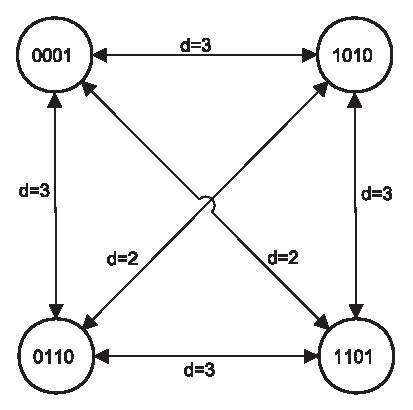
\includegraphics[height=3.0in]{c_eds0/exe001.eps}
\caption{Graphical Solution To Exercise \ref{exe:cedc0:sexe0:01}}
\label{fig:ceds0:exe01:01}
\end{figure}

The relationships between the four codewords of this code can be
depicted as in Figure \ref{fig:ceds0:exe01:01}.  For example,
the Hamming distance between 0001 and 1010 is 3, and the
Hamming distance between 0110 and 1010 is 2.

Since the minimum Hamming distance $\hat{d}$ is defined as the minimum
Hamming distance between any two codewords, this distance is 2.

\end{vworkexercisesolution}

%%%%%%%%%%%%%%%%%%%%%%%%%%%%%%%%%%%%%%%%%%%%%%%%%%%%%%%%%%%%%%%%%%%%%%%%%%
%%%%%%%%%%%%%%%%%%%%%%%%%%%%%%%%%%%%%%%%%%%%%%%%%%%%%%%%%%%%%%%%%%%%%%%%%%
%%%%%%%%%%%%%%%%%%%%%%%%%%%%%%%%%%%%%%%%%%%%%%%%%%%%%%%%%%%%%%%%%%%%%%%%%%


%\vworkexerciseseparator
%\begin{vworkexercisesolution}{\ref{exe:cedc0:sexe0:01}}
%Placeholder.
%\end{vworkexercisesolution}
\vworkexercisechapterfooter


%%%%%%%%%%%%%%%%%%%%%%%%%%%%%%%%%%%%%%%%%%%%%%%%%%%%%%%%%%%%%%%%%%%%%%%%%%
\vfill
\noindent\begin{figure}[!b]
\noindent\rule[-0.25in]{\textwidth}{1pt}
\begin{tiny}
\begin{verbatim}
$HeadURL: svn://localhost/dtapublic/pubs/books/ucbka/trunk/c_eds0/c_eds0.tex $
$Revision: 277 $
$Date: 2019-08-12 22:35:39 -0400 (Mon, 12 Aug 2019) $
$Author: dashley $
\end{verbatim}
\end{tiny}
\noindent\rule[0.25in]{\textwidth}{1pt}
\end{figure}

%%%%%%%%%%%%%%%%%%%%%%%%%%%%%%%%%%%%%%%%%%%%%%%%%%%%%%%%%%%%%%%%%%%%%%%%%%
%
%End of file C_EDS0.TEX


%Chapter:  Solutions:  Boolean Algebra And Simplification Of Boolean Functions
\chapter[Solutions: Chapter \ref{cbal0}]
        {Solutions: Chapter \ref{cbal0}, \cbalzerolongtitle{}}

\label{cbas0}

TBD.

%End of file c_bas0.tex



%Chapter:  Solutions:  Classical And Simple Integer Algorithms And Techniques
%$Header: svn://localhost/dtapublic/pubs/books/ucbka/trunk/c_cis0/c_cis0.tex 277 2019-08-13 02:35:39Z dashley $

\chapter[Solutions: \ccilzeroxrefcomma{}Chapter \ref{ccil0}]
        {Solutions: \ccilzeroxrefcomma{}Chapter \ref{ccil0}, \ccilzerolongtitle{}}

\label{ccis0}

\vworkexercisechapterheader{}
\begin{vworkexercisesolution}{\ref{exe:ccil0:sexe0:01}}
We can show this result in two ways.  The first way, based on bit patterns, is to note
that adding an $m$-bit number, $u$, to its one's complement will result in a bit pattern
containing all 1's, i.e. $\forall i$, $u_{[i]} = 1$.  Adding 1 to this bit pattern will
always produce $\forall i$, $u_{[i]} = 0$ with a carry out.  Since the order of addition
does not matter, this establishes that adding $u$ to $\sim{}u+1$ will produce 0, thus showing
that $u$ and $\sim{}u+1$ are additive inverses.  This method, although valid, does not 
establish that $u$ and $\sim{}u+1$ actually represent additive inverses.  For example, if
$u=-2^{m-1}$, $u=\sim{}u+1$, and clearly a non-zero number cannot be an additive inverse of
itself.  Thus, it would be more comforting to show this result in a way that demonstrates the
actual values of the integers represented.

We present a second method now.  Assume that $u \neq -2^{m-1}$, since 
$-2^{m-1}$ cannot have an additive inverse in an $m$-bit signed integer.
If $u=0$, $\sim{}u+1=0$, so the relationship is clearly met.  If $u<0$, then
$u_{[m-1]}=1$, and by
(\ccilzeroxrefhyphen\ref{eq:ccil0:sroi0:sros0:00}),


\end{vworkexercisesolution}
\vworkexercisechapterfooter

%%%%%%%%%%%%%%%%%%%%%%%%%%%%%%%%%%%%%%%%%%%%%%%%%%%%%%%%%%%%%%%%%%%%%%%%%%
\vfill
\noindent\begin{figure}[!b]
\noindent\rule[-0.25in]{\textwidth}{1pt}
\begin{tiny}
\begin{verbatim}
$HeadURL: svn://localhost/dtapublic/pubs/books/ucbka/trunk/c_cis0/c_cis0.tex $
$Revision: 277 $
$Date: 2019-08-12 22:35:39 -0400 (Mon, 12 Aug 2019) $
$Author: dashley $
\end{verbatim}
\end{tiny}
\noindent\rule[0.25in]{\textwidth}{1pt}
\end{figure}
%%%%%%%%%%%%%%%%%%%%%%%%%%%%%%%%%%%%%%%%%%%%%%%%%%%%%%%%%%%%%%%%%%%%%%%%%%
%
%End of file C_CIS0.TEX


%Chapter:  Solutions:  Rational Approximation
\chapter[Solutions: Chapter \ref{crat0}]
        {Solutions: Chapter \ref{crat0}, \cratzerolongtitle{}}

\label{cras0}

\vworkexercisechapterheader{}
\begin{vworkexercisesolution}{\ref{exe:crat0:sexe0:01}}
The value of the \texttt{state} variable when 
evaluating the \emph{if()} clause on the
$n+1$'th invocation is

\begin{equation}
\label{eq:cras0:exe01:01}
K_1 - nK_4 + (n+1) K_2 .
\end{equation}

We require on the $n+1$'th invocation, in order for the 
test of the \emph{if()} clause to fail (i.e. that the function
``\texttt{A()}'' has been run on the first $n$ invocations of
the base subroutine but is not run on the $n+1$'th invocation), 
that:

\begin{equation}
\label{eq:cras0:exe01:01b}
K_1 - nK_4 + (n+1) K_2 < K_3.
\end{equation}

Solving this inequality for the smallest integral
value of $n$ yields:

\begin{equation}
\label{eq:cras0:exe01:01c}
n = \left\lceil
\frac{K_1 + K_2 - K_3 + 1}{K_4 - K_2}
\right\rceil .
\end{equation}

It can be verified using an example that 
(\ref{eq:cras0:exe01:01c}).  For example, with
$K_1 = 10$, $K_2 = 3$, $K_3 = 7$, and $K_4 = 5$, 
(\ref{eq:cras0:exe01:01}) predicts that on the first
$\lceil 7/2 \rceil = 4$ invocations of the base subroutine
the subroutine ``\texttt{A()}'' will be run but on the 5th
invocation it will not.  Tracing the algorithm with the
parameters specified reveals that at the
test in the \emph{if()} statement 
on the first invocation of the
subroutine, \texttt{state}=13 (``\texttt{A()}'' executed);
on the second invocation of the
subroutine, \texttt{state}=11 (``\texttt{A()}'' executed);
on the third invocation of the
subroutine, \texttt{state}=9 (``\texttt{A()}'' executed);
on the fourth invocation of the
subroutine, \texttt{state}=7 (``\texttt{A()}'' executed);
and on the fifth invocation of the
subroutine, \texttt{state}=5 (``\texttt{A()}'' not executed).
This is in agreement with
(\ref{eq:cras0:exe01:01}). 
\end{vworkexercisesolution}
%\vworkexerciseseparator
%\begin{vworkexercisesolution}{\ref{exe:cfry0:sexe0:02}}
%Placeholder.
%\end{vworkexercisesolution}
\vworkexercisechapterfooter


%%%%%%%%%%%%%%%%%%%%%%%%%%%%%%%%%%%%%%%%%%%%%%%%%%%%%%%%%%%%%%%%%%%%%%%%%%
%End of file c_ras0.tex



% New part: Glossaries, Bibliography, And Index
\part{Glossaries, Bibliography, And Index}

%Mark the start of appendices.  This causes numbering to be with letters
%instead of numbers.
\appendix

%Glossary Of Terms
\cleardoublepage
\addcontentsline{toc}{chapter}{Glossary Of Terms}
\chapter*{Glossary Of Terms}
\markboth{GLOSSARY OF TERMS}{GLOSSARY OF TERMS}

\label{cglo0}

\begin{vworktermglossaryenum}

\item \textbf{axiom}\index{axiom}

      A statement used in the premises of arguments and assumed to be true
	  without proof.  In some cases axioms are held to be self-evident, as in 
	  Euclidian geometry, while in others they are assumptions put forward for
	  the sake of argument.
      (Taken verbatim from \cite{bibref:b:penguindictionaryofmathematics:2ded}.)

\item \textbf{cardinality}\index{cardinality}

      The cardinality of a set is the
      number of elements in the set.  In this work, the cardinality
      of a set is denoted $n()$.  For example, 
      $n(\{12,29,327\}) = 3$.

\item \textbf{coprime}\index{coprime}

      Two integers that share no prime factors are \emph{coprime}.
      \emph{Example:}
      6 and 7 are coprime, whereas 6 and 8 are not.

\item \textbf{GMP}\index{GMP}

      The \emph{G}NU \emph{M}ultiple \emph{P}recision library.
      The GMP is an arbitrary-precision integer, rational number,
      and floating-point library that places no restrictions on
      size of integers or number of significant digits in floating-point
      numbers.  This 
      library is famous because it is the fastest of its
      kind, and generally uses asymptotically superior algorithms.

\item \textbf{greatest common divisor (g.c.d.)}

      The greatest common divisor of two integers is the largest
      integer which divides both integers without a remainder.
      \emph{Example:} the g.c.d. of 30 and 42 is 6.

\item \textbf{integer}\index{integer}\index{sets of integers}\index{Z@$\vworkintset$}%
      \index{integer!Z@$\vworkintset$}\index{integer!sets of}

      (Nearly verbatim from \cite{bibref:w:wwwwhatiscom}) An \emph{integer}
      (pronounced \emph{IN-tuh-jer}) is a whole number
      (not a fractional number) that can be positive, negative, or zero. 

      Examples of integers are: -5, 1, 5, 8, 97, and 3,043. 

      Examples of numbers that are not integers are: -1.43, 1 3/4, 3.14, 
      0.09, and 5,643.1. 

      The set of integers, denoted $\vworkintset{}$, is formally defined as:

      \begin{equation}
      \vworkintset{} = \{\ldots{}, -3, -2, -1, 0, 1, 2, 3, \ldots{} \}
      \end{equation}

      In mathematical equations, unknown or unspecified integers are 
      represented by lowercase, italicized letters from the 
      ``late middle'' of the alphabet.  The most common 
      are $p$, $q$, $r$, and $s$.

\item \textbf{irreducible}

      A rational number $p/q$ where $p$ and $q$ are coprime
      is said to be \emph{irreducible}.
      Equivalently, it may be stated that $p$ and $q$ share no prime factors
      or that the greatest common divisor of
      $p$ and $q$ is 1.

\item \textbf{KPH}

      Kilometers per hour.

\item \textbf{limb}\index{limb}

      An integer of a size which a machine can manipulate natively
      that is arranged in an array to create a larger
      integer which the machine cannot manipulate natively and must be
      manipulated through arithmetic subroutines.

\item \textbf{limbsize}\index{limbsize}

      The size, in bits, of a limb.  The limbsize usually represents
      the size of integer that a machine can manipulate directly
      through machine instructions.  For an inexpensive microcontroller,
      8 or 16 is a typical limbsize.  For a personal computer or 
      workstation, 32 or 64 is a typical limbsize.

\item \textbf{MPH}

      Miles per hour.

\item \textbf{mediant}\index{mediant}

      The mediant of two fractions $m/n$ and $m'/n'$ is the fraction 
	  $\frac{m+m'}{n+n'}$ (see Definition 
	  \ref{def:cfry0:spfs:02}).  Note that the
	  mediant of two fractions with non-negative integer components
	  is always between them, but not usually exactly at the 
	  midpoint (see Lemma \ref{lem:cfry0:spfs:02c}).

\item \textbf{natural number}\index{natural number}\index{integer!natural number}%
      \index{sets of integers}\index{N@$\vworkintsetpos$}%
      \index{integer!N@$\vworkintsetpos$}\index{integer!sets of}
         
      (Nearly verbatim from \cite{bibref:w:wwwwhatiscom})
      A \emph{natural number}
      is a number that occurs commonly and obviously in nature.  
      As such, it is a whole, non-negative number.  
      The set of natural numbers, denoted $\vworkintsetpos{}$, 
      can be defined in either of two ways:

      \begin{equation}
      \label{cglo0:eq0001}
      \vworkintsetpos{} = \{ 0, 1, 2, 3, \ldots{} \}
      \end{equation}

      \begin{equation}
      \label{cglo0:eq0002}
      \vworkintsetpos{} = \{ 1, 2, 3, 4, \ldots{} \}
      \end{equation}
      
      In mathematical equations, unknown or unspecified natural numbers 
      are represented by lowercase, italicized letters from the 
      middle of the alphabet.  The most common is $n$, followed by 
      $m$, $p$, and $q$.  
      In subscripts, the lowercase $i$ is sometimes used to represent 
      a non-specific natural number when denoting the elements in a 
      sequence or series.  However, $i$ is more often used to represent 
      the positive square root of -1, the unit imaginary number.

      \textbf{Important Note:}  The definition above is reproduced nearly
      verbatim from \cite{bibref:w:wwwwhatiscom}, and (\ref{cglo0:eq0001})
      is supplied only for perspective.  In this work, a natural
      number is defined by (\ref{cglo0:eq0002}) rather than (\ref{cglo0:eq0001}).
      In this work, the set of non-negative integers is denoted by
      $\vworkintsetnonneg{}$ rather than $\vworkintsetpos{}$.\index{Z+@$\vworkintsetnonneg$}%
      \index{integer!Z+@$\vworkintsetnonneg$}\index{integer!non-negative}

\item \textbf{postulate}\index{postulate!definition}

      An axiom (see \emph{axiom} earlier in this glossary).  The term is usually
	  used in certain contexts, e.g. Euclid's postulates or Peano's postulates.
	  (Taken verbatim from \cite{bibref:b:penguindictionaryofmathematics:2ded}.)

\item \textbf{prime number}\index{prime number!definition}

      (Nearly verbatim from \cite{bibref:w:wwwwhatiscom}) A \emph{prime number}
      is a whole number greater than 1, whose only two whole-number 
      factors are 1 and itself.  The first few prime numbers are 
      2, 3, 5, 7, 11, 13, 17, 19, 23, and 29.  As we proceed in the set of 
      natural numbers $\vworkintsetpos{} = \{ 1, 2, 3, \ldots{} \} $, the 
      primes become less and less frequent in general.  
      However, there is no largest prime number.  
      For every prime number $p$, there exists a prime number $p'$ such that 
      $p'$ is greater than $p$.  This was demonstrated in ancient times by the 
      Greek mathematician \index{Euclid}Euclid.\index{prime number!no largest prime number}%
      \index{Euclid!Second Theorem}

      Suppose $n$ is a whole number, and we want to test it to see if it is prime.   
      First, we take the square root (or the 1/2 power) of $n$; then we round this 
      number up to the next highest whole number.  Call the result $m$.  
      We must find all of the following quotients:

      \begin{equation}
      \begin{array}{rcl}
         q_m     & =        & n / m              \\
         q_{m-1} & =        & n / (m-1)          \\
         q_{m-2} & =        & n / (m-2)          \\
         q_{m-3} & =        & n / (m-3)          \\
                 & \ldots{} &                    \\
         q_3     & =        & n / 3              \\
         q_2     & =        & n / 2              \\
      \end{array}
      \end{equation}

      The number $n$ is prime if and only if none of the $q$'s, as 
      derived above, are whole numbers.

      A computer can be used to test extremely large numbers to see if they are prime.  
      But, because there is no limit to how large a natural number can be, 
      there is always a point where testing in this manner becomes too great 
      a task even for the most powerful supercomputers.  
      Various algorithms have been formulated in an attempt to generate 
      ever-larger prime numbers.  These schemes all have limitations.

\end{vworktermglossaryenum}

%End of file c_glo0.tex


%
%Glossary Of Mathematical Notation
\cleardoublepage
\addcontentsline{toc}{chapter}{Glossary Of Mathematical Notation}
%$Header: /home/dashley/cvsrep/uculib01/uculib01/doc/manual/c_glo1/c_glo1.tex,v 1.2 2010/01/28 21:18:32 dashley Exp $

\chapter{Glossary Of Mathematical And Other Notation}
\markboth{GLOSSARY OF MATHEMATICAL NOTATION}{GLOSSARY OF MATHEMATICAL NOTATION}

\label{cglo1}

%%%%%%%%%%%%%%%%%%%%%%%%%%%%%%%%%%%%%%%%%%%%%%%%%%%%%%%%%%%%%%%%%%%%%%%%%%%%%%%
%%%%%%%%%%%%%%%%%%%%%%%%%%%%%%%%%%%%%%%%%%%%%%%%%%%%%%%%%%%%%%%%%%%%%%%%%%%%%%%
%%%%%%%%%%%%%%%%%%%%%%%%%%%%%%%%%%%%%%%%%%%%%%%%%%%%%%%%%%%%%%%%%%%%%%%%%%%%%%%

\section*{General Notation}

\begin{vworkmathtermglossaryenum}

\item \mbox{\boldmath $ \vworkdivides $}


      $a \vworkdivides b$, 
      \index{divides@divides ($\vworkdivides$)}
      \index{--@$\vworkdivides$ (divides)}
      read ``\emph{$a$ divides $b$}'', denotes that $b/a$ has no remainder.
      Equivalently, it may be stated that
      $(a \vworkdivides b) \Rightarrow (\exists c \in \vworkintset{}, b = ac)$.

\item \mbox{\boldmath $ \vworknotdivides $}

      $a \vworknotdivides b$, 
      \index{divides@divides ($\vworkdivides$)}
      \index{--@$\vworknotdivides$ (doesn't divide)}
      read ``\emph{$a$ does not divide $b$}'', denotes that $b/a$ has a reminder.
      Equivalently, it may be stated that
      $(a \vworknotdivides b) \Rightarrow (\nexists c \in \vworkintset{}, b = ac)$.

\item \mbox{\boldmath $ \lfloor \cdot \rfloor $}

      Used
      \index{floor function@floor function ($\lfloor\cdot\rfloor$)}
      \index{--@$\lfloor\cdot\rfloor$ (\emph{floor($\cdot$)} function)}
      to denote the \emph{floor($\cdot$)} function.  The
      \emph{floor($\cdot$)}
      function is the largest integer not larger than the
      argument.

\item \mbox{\boldmath $\lceil \cdot \rceil$ }

      Used
      \index{ceiling function@ceiling function ($\lceil\cdot\rceil$)}
      \index{--@$\lceil\cdot\rceil$ (\emph{ceiling($\cdot$)} function)}
      to denote the \emph{ceiling($\cdot$)} function.
      The \emph{ceiling($\cdot$)} function
      is the smallest integer not smaller than the
      argument.
\end{vworkmathtermglossaryenum}

%%%%%%%%%%%%%%%%%%%%%%%%%%%%%%%%%%%%%%%%%%%%%%%%%%%%%%%%%%%%%%%%%%%%%%%%%%%%%%%
%%%%%%%%%%%%%%%%%%%%%%%%%%%%%%%%%%%%%%%%%%%%%%%%%%%%%%%%%%%%%%%%%%%%%%%%%%%%%%%
%%%%%%%%%%%%%%%%%%%%%%%%%%%%%%%%%%%%%%%%%%%%%%%%%%%%%%%%%%%%%%%%%%%%%%%%%%%%%%%

\section*{Usage Of English And Greek Letters}

\begin{vworkmathtermglossaryenum}

\item \mbox {\boldmath $a/b$}

      An arbitrary \index{rational number}rational number.

\item \mbox {\boldmath $ F_N $}

      The \index{Farey series}Farey 
      series of order $N$.  The Farey series is the
      ordered set of irreducible rational numbers 
          in [0,1] with a
      denominator not larger than $N$.

\item \mbox {\boldmath $F_{k_{MAX}, \overline{h_{MAX}}}$}
      
          \index{FKMAXHMAX@$F_{k_{MAX}, \overline{h_{MAX}}}$}
          The ordered set of irreducible rational numbers
          $h/k$ subject to the constraints $0 \leq h \leq h_{MAX}$
          and $1 \leq k \leq h_{MAX}$.  
%         (See Section \cfryzeroxrefhyphen{}\ref{cfry0:schk0}.)


\item \mbox{\boldmath $H/K$}, \mbox{\boldmath $h/k$},
      \mbox{\boldmath $h'/k'$}, \mbox{\boldmath $h''/k''$},
      \mbox{\boldmath $h_i/k_i$}

      Terms in a Farey series of order $N$.

\item \mbox{\boldmath $r_A$}

      The rational number $h/k$ used to approximate
      an arbitrary real number $r_I$.

\item \mbox{\boldmath $r_I$}

      The real number, which may or may not be rational,
      which is to be approximated by a rational number
      $r_A = h/k$.

\item \textbf{reduced}

      See \emph{irreducible}.

\item \mbox{\boldmath $s_k = p_k/q_k$}

      The $k$th convergent of a continued fraction.

\item \mbox{\boldmath $x_{MAX}$}

      The largest element of the domain for which the
      behavior of an approximation must be guaranteed.
      In this paper, most derivations assume
      that $x \in [0, x_{MAX}]$, $x_{MAX} \in \vworkintsetpos{}$.
\end{vworkmathtermglossaryenum}

%%%%%%%%%%%%%%%%%%%%%%%%%%%%%%%%%%%%%%%%%%%%%%%%%%%%%%%%%%%%%%%%%%%%%%%%%%%%%%%
%%%%%%%%%%%%%%%%%%%%%%%%%%%%%%%%%%%%%%%%%%%%%%%%%%%%%%%%%%%%%%%%%%%%%%%%%%%%%%%
%%%%%%%%%%%%%%%%%%%%%%%%%%%%%%%%%%%%%%%%%%%%%%%%%%%%%%%%%%%%%%%%%%%%%%%%%%%%%%%

\section*{Bitfields And Portions Of Integers}

\begin{vworkmathtermglossaryenum}
\item \mbox{\boldmath $a_{b}$}

      The $b$th bit of the integer $a$.  Bits are numbered with the
      least significant bit ``0'', and consecutively through 
      ``$n-1$'', where $n$ is the total number of bits.

      In general, if $p$ is an $n$-bit unsigned integer,

      \begin{equation}
      \nonumber p = \sum_{i=0}^{n-1} 2^i p_i .
      \end{equation}

\item \mbox{\boldmath $a_{c:b}$}

      The integer consisting of the $b$th through the
      $c$th bits of the integer $a$.  Bits are numbered with the
      least significant bit ``0'', and consecutively through 
      ``$n-1$'', where $n$ is the total number of bits.

      For example, if $p$ is a 24-bit unsigned integer, then

      \begin{equation}
      \nonumber p = 2^{16}p_{23:16} + 2^{8}p_{15:8} + p_{7:0} .
      \end{equation}

\item \mbox{\boldmath $a_{[b]}$}

      The $b$th word of the integer $a$.  Words are numbered 
      with the
      least significant word ``0'', and consecutively through 
      ``$n-1$'', where $n$ is the total number of words.

      In general, if $p$ is an $n$-word unsigned integer 
      and $z$ is the wordsize in bits,

      \begin{equation}
      \nonumber p = \sum_{i=0}^{n-1} 2^{iz} p_i .
      \end{equation}

\item \mbox{\boldmath $a_{[c:b]}$}

      The integer consisting of the $b$th through the
      $c$th word of the integer $a$.  Words are numbered with the
      least significant word ``0'', and consecutively through 
      ``$n-1$'', where $n$ is the total number of words.

      For example, if $p$ is a 24-word unsigned integer and
      $z$ is the wordsize in bits, then

      \begin{equation}
      \nonumber p = 2^{16z}p_{[23:16]} + 2^{8z}p_{[15:8]} + p_{[7:0]} .
      \end{equation}

\end{vworkmathtermglossaryenum}

%%%%%%%%%%%%%%%%%%%%%%%%%%%%%%%%%%%%%%%%%%%%%%%%%%%%%%%%%%%%%%%%%%%%%%%%%%%%%%%
%%%%%%%%%%%%%%%%%%%%%%%%%%%%%%%%%%%%%%%%%%%%%%%%%%%%%%%%%%%%%%%%%%%%%%%%%%%%%%%
%%%%%%%%%%%%%%%%%%%%%%%%%%%%%%%%%%%%%%%%%%%%%%%%%%%%%%%%%%%%%%%%%%%%%%%%%%%%%%%

\section*{Matrices And Vectors}

\begin{vworkmathtermglossaryenum}

\item \mbox{\boldmath $0$}

      $\mathbf{0}$ (in bold face) is used to denote either a vector or matrix
      populated with all zeroes.  Optionally, in cases where the context is not clear
      or where there is cause to highlight the dimension, $\mathbf{0}$ may be subscripted
      to indicate the dimension, i.e. 
      
      \begin{equation}
      \nonumber
      \mathbf{0}_3 = \left[\begin{array}{c} 0 \\ 0 \\ 0 \end{array}\right]
      \end{equation}

      \begin{equation}
      \nonumber
      \mathbf{0}_{3 \times 2} = \left[\begin{array}{cc} 0&0 \\ 0&0 \\ 0&0 \end{array}\right]
      \end{equation}

\item \mbox{\boldmath $I$}

      $I$ is used to denote the square identity matrix (the matrix with all
      elements 0 except elements on the diagonal which are 1).
      Optionally, in cases where the context is not clear
      or where there is cause to highlight the dimension, $I$ may be subscripted
      to indicate the dimension, i.e. 
      
      \begin{equation}
      \nonumber
      I = I_3 = I_{3 \times 3} = \left[\begin{array}{ccc} 1&0&0 \\ 0&1&0 \\ 0&0&1 \end{array}\right]
      \end{equation}

\end{vworkmathtermglossaryenum}


%%%%%%%%%%%%%%%%%%%%%%%%%%%%%%%%%%%%%%%%%%%%%%%%%%%%%%%%%%%%%%%%%%%%%%%%%%%%%%%
%%%%%%%%%%%%%%%%%%%%%%%%%%%%%%%%%%%%%%%%%%%%%%%%%%%%%%%%%%%%%%%%%%%%%%%%%%%%%%%
%%%%%%%%%%%%%%%%%%%%%%%%%%%%%%%%%%%%%%%%%%%%%%%%%%%%%%%%%%%%%%%%%%%%%%%%%%%%%%%

\section*{Sets And Set Notation}

\begin{vworkmathtermglossaryenum}

\item \mbox{\boldmath $n(A)$}

      The \index{cardinality}cardinality of set $A$.  (The cardinality of a set is the
      number of elements in the set.)

\end{vworkmathtermglossaryenum}

%%%%%%%%%%%%%%%%%%%%%%%%%%%%%%%%%%%%%%%%%%%%%%%%%%%%%%%%%%%%%%%%%%%%%%%%%%%%%%%
%%%%%%%%%%%%%%%%%%%%%%%%%%%%%%%%%%%%%%%%%%%%%%%%%%%%%%%%%%%%%%%%%%%%%%%%%%%%%%%
%%%%%%%%%%%%%%%%%%%%%%%%%%%%%%%%%%%%%%%%%%%%%%%%%%%%%%%%%%%%%%%%%%%%%%%%%%%%%%%

\section*{Sets Of Numbers}

\begin{vworkmathtermglossaryenum}

\item \mbox{\boldmath $\vworkintsetpos$}

      The 
      \index{natural number}
      \index{N@$\vworkintsetpos$}
      set of positive integers (natural numbers).

\item \mbox{\boldmath $\vworkratset$}

      The 
      \index{rational number}
      \index{Q@$\vworkratset$}
      set of rational numbers.

\item \mbox{\boldmath $\vworkratsetnonneg$}

      The 
      \index{rational number}
      \index{Q+@$\vworkratsetnonneg$}
      set of non-negative rational numbers.

\item \mbox{\boldmath $\vworkrealset$}

      The 
      \index{real number}
      \index{R@$\vworkrealset$}
      set of real numbers.

\item \mbox{\boldmath $\vworkrealsetnonneg$}

      The 
      \index{real number}
      \index{R+@$\vworkrealsetnonneg$}
      set of non-negative real numbers.

\item \mbox{\boldmath $\vworkintset$}

      The 
      \index{integer}
      \index{Z@$\vworkintset$}
      set of integers.

\item \mbox{\boldmath $\vworkintsetnonneg$}

      The 
      \index{integer}
      \index{Z+@$\vworkintsetnonneg$}
      set of non-negative integers.

\end{vworkmathtermglossaryenum}


%%%%%%%%%%%%%%%%%%%%%%%%%%%%%%%%%%%%%%%%%%%%%%%%%%%%%%%%%%%%%%%%%%%%%%%%%%%%%%%
%%%%%%%%%%%%%%%%%%%%%%%%%%%%%%%%%%%%%%%%%%%%%%%%%%%%%%%%%%%%%%%%%%%%%%%%%%%%%%%
%%%%%%%%%%%%%%%%%%%%%%%%%%%%%%%%%%%%%%%%%%%%%%%%%%%%%%%%%%%%%%%%%%%%%%%%%%%%%%%

\noindent\begin{figure}[!b]
\noindent\rule[-0.25in]{\textwidth}{1pt}
\begin{tiny}
\begin{verbatim}
$RCSfile: c_glo1.tex,v $
$Source: /home/dashley/cvsrep/uculib01/uculib01/doc/manual/c_glo1/c_glo1.tex,v $
$Revision: 1.2 $
$Author: dashley $
$Date: 2010/01/28 21:18:32 $
\end{verbatim}
\end{tiny}
\noindent\rule[0.25in]{\textwidth}{1pt}
\end{figure}

%%%%%%%%%%%%%%%%%%%%%%%%%%%%%%%%%%%%%%%%%%%%%%%%%%%%%%%%%%%%%%%%%%%%%%%%%%%%%%%
%$Log: c_glo1.tex,v $
%Revision 1.2  2010/01/28 21:18:32  dashley
%a)Chapter start quotes removed.
%b)Aesthetic comment line added at the bottom of most files.
%
%Revision 1.1  2007/08/30 14:43:38  dtashley
%Initial checkin.
%
%End of file $RCSfile: c_glo1.tex,v $.
%%%%%%%%%%%%%%%%%%%%%%%%%%%%%%%%%%%%%%%%%%%%%%%%%%%%%%%%%%%%%%%%%%%%%%%%%%%%%%%


%
%Bibliography
\cleardoublepage
\addcontentsline{toc}{chapter}{Bibliography}
%$Header: /home/dashley/cvsrep/e3ft_gpl01/e3ft_gpl01/webprojs/pamc/gen_a/docs/manual/man_a/comps/workbibl.tex,v 1.3 2009/10/31 20:02:15 dashley Exp $

%Legend
%    b - book
%    c - company
%    d - document
%    i - individual, i.e. person
%    n - newsgroup
%    p - paper
%    s - software, software distributions
%    w - web page.
%
%%%%%%%%%%%%%%%%%%%%%%%%%%%%%%%%%%%%%%%%%%%%%%%%%%%%%%%%%%%%%%%%%%%%%%%%%%
\chapter*{Bibliography}

\markboth{BIBLIOGRAPHY}{BIBLIOGRAPHY}

\newcounter{custombibcounter}

\nocite{*}

%%%%%%%%%%%%%%%%%%%%%%%%%%%%%%%%%%%%%%%%%%%%%%%%%%%%%%%%%%%%%%%%%%%%%%%%%%

\section*{Two-Factor Authentication Vendors}
\index{two-factor authentication}

\begin{thecustombibliography}{9999}

\bibitem{bibref:c:cryptocardcorporation}
CryptoCard Corporation,\index{CryptoCard Corporation}\\
\texttt{http://www.cryptocard.com}

\end{thecustombibliography}


%%%%%%%%%%%%%%%%%%%%%%%%%%%%%%%%%%%%%%%%%%%%%%%%%%%%%%%%%%%%%%%%%%%%%%%%%%

\section*{Corporations and Organizations}

\begin{thecustombibliography}{9999}

\bibitem{bibref:c:cequentelectricalproducts}
Cequent Electrical Products\index{Cequent Electrical Products}\\
101 Spires Parkway, Tekonsha, Michigan, USA, 49092\\
\texttt{http://www.cequentgroup.com}

\end{thecustombibliography}

%%%%%%%%%%%%%%%%%%%%%%%%%%%%%%%%%%%%%%%%%%%%%%%%%%%%%%%%%%%%%%%%%%%%%%%%%%

\section*{Individuals}

\begin{thecustombibliography}{9999}

\bibitem{bibref:i:marciaalbright}
Marcia Albright,\index{Albright, Marcia}
E-mail: \texttt{malbright@cequentgroup.com}

\bibitem{bibref:i:johncebasek}
John Cebasek,\index{Cebasek, John}
E-mail: \texttt{john.cebasek@cryptocard.com}

\bibitem{bibref:i:billlaham}
Bill LaHam,\index{LaHam, Bill}
E-mail: \texttt{bill.laham@cryptocard.com}

\bibitem{bibref:i:dougmotts}
Doug Motts,\index{Motts, Doug}
E-mail: \texttt{dmotts@cequentgroup.com}

\end{thecustombibliography}

%%%%%%%%%%%%%%%%%%%%%%%%%%%%%%%%%%%%%%%%%%%%%%%%%%%%%%%%%%%%%%%%%%%%%%%%%%

\noindent\begin{figure}[!b]
\noindent\rule[-0.25in]{\textwidth}{1pt}
\begin{tiny}
\begin{verbatim}
$RCSfile: workbibl.tex,v $
$Source: /home/dashley/cvsrep/e3ft_gpl01/e3ft_gpl01/webprojs/pamc/gen_a/docs/manual/man_a/comps/workbibl.tex,v $
$Revision: 1.3 $
$Author: dashley $
$Date: 2009/10/31 20:02:15 $
\end{verbatim}
\end{tiny}
\noindent\rule[0.25in]{\textwidth}{1pt}
\end{figure}

%%%%%%%%%%%%%%%%%%%%%%%%%%%%%%%%%%%%%%%%%%%%%%%%%%%%%%%%%%%%%%%%%%%%%%%%%%%%%%%
% $Log: workbibl.tex,v $
% Revision 1.3  2009/10/31 20:02:15  dashley
% Edits.
%
% Revision 1.2  2007/06/03 04:57:47  dashley
% Checkin to be sure that changes wrapped up in weekly TAR.GZ file.
%
% Revision 1.1  2007/06/03 02:57:45  dashley
% Initial checkin.
%
%End of $RCSfile: workbibl.tex,v $.

%
%Index Must Be Formed At This Directory Level
\cleardoublepage
\addcontentsline{toc}{chapter}{Index}
\printindex
%
\end{document}
%
%End of file SVF.TEX.
